\documentclass[a4paper,11pt,twoside]{article}

%%% packages:
\usepackage[T1]{fontenc}
\usepackage{ucs}
\usepackage[utf8x]{inputenc}
%\usepackage[frenchb]{babel}
\usepackage{amsmath}
\usepackage{amssymb}
\usepackage{latexsym}
\usepackage{verbatim}
\usepackage{moreverb}
\usepackage{fancyvrb}
\usepackage{alltt}
\usepackage{eurosym}
\usepackage{hyperref}
\usepackage{colortbl}
\usepackage{graphicx}
\usepackage{pdflscape}
\usepackage{afterpage}
\usepackage{rotating}
\usepackage{tikz}
%\usepackage{tikz-qtree}

%%% Geometry (https://en.wikibooks.org/wiki/LaTeX/Page_Layout)
\usepackage{layout}
%\usepackage[a4paper,top=1in, bottom=1.25in, left=1.25in, right=1.25in, inner=4cm,outer=2cm]{geometry}
\usepackage[a4paper,inner=2cm,outer=2cm]{geometry}
%% \setlength{\hoffset}{-1inch}
%% \setlength{\voffset}{-1inch0pt}
\setlength{\textheight}{23cm}
%% \setlength{\textwidth}{18cm}

%%% macros:
\newcommand{\thepath}{.}
\newcommand{\imgpath}{\thepath/images}
\newcommand{\pdfteximgpath}{\thepath/pdftex}
\newcommand{\pdftextimgpath}{\thepath/pdftex_t}

%%%
\title{The SuperNEMO Vire-CMS/LAPP interface\\version 0.7}
\author{E.Chabanne, J.Hommet, T. Leflour, Y. Lemière,
  S.Lieunard, F.Mauger, J.-L. Panazol, J.Poincheval}
\date{\today}

%%%
\begin{document}

\thispagestyle{empty}
%\layout{}
\maketitle
\begin{abstract}
This document aims  to describe the requirements of  the Vire CMS/LAPP
interface,  i.e. the  software bridge  between the  Vire based  online
software  (Vire server  and clients,  a.k.a the  Vire system)  and the
CMS/LAPP server  that plays  the role  of the  unique gate  (subcontractor proxy) to
communicate with  the OPCUA-based MOS  servers responsible of  the low
level control and monitoring operations on some hardware devices.
\end{abstract}
\vfill
\pagebreak

\tableofcontents
\vfill
\pagebreak

\listoffigures
\vfill
\pagebreak

\listoftables
\vfill
\pagebreak
\clearpage

\documentclass[a4paper,11pt,twoside]{article}

%%% packages:
\usepackage[T1]{fontenc}
\usepackage{ucs}
\usepackage[utf8x]{inputenc}
%\usepackage[frenchb]{babel}
\usepackage{amsmath}
\usepackage{amssymb}
\usepackage{latexsym}
\usepackage{verbatim}
\usepackage{moreverb}
\usepackage{fancyvrb}
\usepackage{alltt}
\usepackage{eurosym}
\usepackage{hyperref}
\usepackage{colortbl}
\usepackage{graphicx}
\usepackage{pdflscape}
\usepackage{afterpage}
\usepackage{rotating}
\usepackage{tikz}
%\usepackage{tikz-qtree}

%%% Geometry (https://en.wikibooks.org/wiki/LaTeX/Page_Layout)
\usepackage{layout}
%\usepackage[a4paper,top=1in, bottom=1.25in, left=1.25in, right=1.25in, inner=4cm,outer=2cm]{geometry}
\usepackage[a4paper,inner=2cm,outer=2cm]{geometry}
%% \setlength{\hoffset}{-1inch}
%% \setlength{\voffset}{-1inch0pt}
\setlength{\textheight}{23cm}
%% \setlength{\textwidth}{18cm}

%%% macros:
\newcommand{\thepath}{.}
\newcommand{\imgpath}{\thepath/images}
\newcommand{\pdfteximgpath}{\thepath/pdftex}
\newcommand{\pdftextimgpath}{\thepath/pdftex_t}

%%%
\title{The SuperNEMO Vire-CMS/LAPP interface\\version 0.7}
\author{E.Chabanne, J.Hommet, T. Leflour, Y. Lemière,
  S.Lieunard, F.Mauger, J.-L. Panazol, J.Poincheval}
\date{\today}

%%%
\begin{document}

\thispagestyle{empty}
%\layout{}
\maketitle
\begin{abstract}
This document aims  to describe the requirements of  the Vire CMS/LAPP
interface,  i.e. the  software bridge  between the  Vire based  online
software  (Vire server  and clients,  a.k.a the  Vire system)  and the
CMS/LAPP server  that plays  the role  of the  unique gate  (subcontractor proxy) to
communicate with  the OPCUA-based MOS  servers responsible of  the low
level control and monitoring operations on some hardware devices.
\end{abstract}
\vfill
\pagebreak

\tableofcontents
\vfill
\pagebreak

\listoffigures
\vfill
\pagebreak

\listoftables
\vfill
\pagebreak
\clearpage

\documentclass[a4paper,11pt,twoside]{article}

%%% packages:
\usepackage[T1]{fontenc}
\usepackage{ucs}
\usepackage[utf8x]{inputenc}
%\usepackage[frenchb]{babel}
\usepackage{amsmath}
\usepackage{amssymb}
\usepackage{latexsym}
\usepackage{verbatim}
\usepackage{moreverb}
\usepackage{fancyvrb}
\usepackage{alltt}
\usepackage{eurosym}
\usepackage{hyperref}
\usepackage{colortbl}
\usepackage{graphicx}
\usepackage{pdflscape}
\usepackage{afterpage}
\usepackage{rotating}
\usepackage{tikz}
%\usepackage{tikz-qtree}

%%% Geometry (https://en.wikibooks.org/wiki/LaTeX/Page_Layout)
\usepackage{layout}
%\usepackage[a4paper,top=1in, bottom=1.25in, left=1.25in, right=1.25in, inner=4cm,outer=2cm]{geometry}
\usepackage[a4paper,inner=2cm,outer=2cm]{geometry}
%% \setlength{\hoffset}{-1inch}
%% \setlength{\voffset}{-1inch0pt}
\setlength{\textheight}{23cm}
%% \setlength{\textwidth}{18cm}

%%% macros:
\newcommand{\thepath}{.}
\newcommand{\imgpath}{\thepath/images}
\newcommand{\pdfteximgpath}{\thepath/pdftex}
\newcommand{\pdftextimgpath}{\thepath/pdftex_t}

%%%
\title{The SuperNEMO Vire-CMS/LAPP interface\\version 0.7}
\author{E.Chabanne, J.Hommet, T. Leflour, Y. Lemière,
  S.Lieunard, F.Mauger, J.-L. Panazol, J.Poincheval}
\date{\today}

%%%
\begin{document}

\thispagestyle{empty}
%\layout{}
\maketitle
\begin{abstract}
This document aims  to describe the requirements of  the Vire CMS/LAPP
interface,  i.e. the  software bridge  between the  Vire based  online
software  (Vire server  and clients,  a.k.a the  Vire system)  and the
CMS/LAPP server  that plays  the role  of the  unique gate  (subcontractor proxy) to
communicate with  the OPCUA-based MOS  servers responsible of  the low
level control and monitoring operations on some hardware devices.
\end{abstract}
\vfill
\pagebreak

\tableofcontents
\vfill
\pagebreak

\listoffigures
\vfill
\pagebreak

\listoftables
\vfill
\pagebreak
\clearpage

\documentclass[a4paper,11pt,twoside]{article}

%%% packages:
\usepackage[T1]{fontenc}
\usepackage{ucs}
\usepackage[utf8x]{inputenc}
%\usepackage[frenchb]{babel}
\usepackage{amsmath}
\usepackage{amssymb}
\usepackage{latexsym}
\usepackage{verbatim}
\usepackage{moreverb}
\usepackage{fancyvrb}
\usepackage{alltt}
\usepackage{eurosym}
\usepackage{hyperref}
\usepackage{colortbl}
\usepackage{graphicx}
\usepackage{pdflscape}
\usepackage{afterpage}
\usepackage{rotating}
\usepackage{tikz}
%\usepackage{tikz-qtree}

%%% Geometry (https://en.wikibooks.org/wiki/LaTeX/Page_Layout)
\usepackage{layout}
%\usepackage[a4paper,top=1in, bottom=1.25in, left=1.25in, right=1.25in, inner=4cm,outer=2cm]{geometry}
\usepackage[a4paper,inner=2cm,outer=2cm]{geometry}
%% \setlength{\hoffset}{-1inch}
%% \setlength{\voffset}{-1inch0pt}
\setlength{\textheight}{23cm}
%% \setlength{\textwidth}{18cm}

%%% macros:
\newcommand{\thepath}{.}
\newcommand{\imgpath}{\thepath/images}
\newcommand{\pdfteximgpath}{\thepath/pdftex}
\newcommand{\pdftextimgpath}{\thepath/pdftex_t}

%%%
\title{The SuperNEMO Vire-CMS/LAPP interface\\version 0.7}
\author{E.Chabanne, J.Hommet, T. Leflour, Y. Lemière,
  S.Lieunard, F.Mauger, J.-L. Panazol, J.Poincheval}
\date{\today}

%%%
\begin{document}

\thispagestyle{empty}
%\layout{}
\maketitle
\begin{abstract}
This document aims  to describe the requirements of  the Vire CMS/LAPP
interface,  i.e. the  software bridge  between the  Vire based  online
software  (Vire server  and clients,  a.k.a the  Vire system)  and the
CMS/LAPP server  that plays  the role  of the  unique gate  (subcontractor proxy) to
communicate with  the OPCUA-based MOS  servers responsible of  the low
level control and monitoring operations on some hardware devices.
\end{abstract}
\vfill
\pagebreak

\tableofcontents
\vfill
\pagebreak

\listoffigures
\vfill
\pagebreak

\listoftables
\vfill
\pagebreak
\clearpage

\input{cms_server/main.tex}
\vfill
\pagebreak
\clearpage

\input{vire_resources/main.tex}
\vfill
\pagebreak
\clearpage

% \input{cmslapp_vireclients/main.tex}
\section{Interaction of the CMS/LAPP server with Vire clients}

TODO
\vfill
\pagebreak
\clearpage

%%%%%%%%%
\appendix

\input{appendix/app_filesystem.tex}
\input{appendix/app_new_device.tex}
\input{appendix/app_vire_messages.tex}
%\input{appendix/app_json_fmt.tex}
\input{appendix/app_protobuf_format.tex}
\input{appendix/app_payload_objects.tex}
\input{appendix/app_rabbitmq_rpc.tex}

\end{document}
%%

\vfill
\pagebreak
\clearpage

\documentclass[a4paper,11pt,twoside]{article}

%%% packages:
\usepackage[T1]{fontenc}
\usepackage{ucs}
\usepackage[utf8x]{inputenc}
%\usepackage[frenchb]{babel}
\usepackage{amsmath}
\usepackage{amssymb}
\usepackage{latexsym}
\usepackage{verbatim}
\usepackage{moreverb}
\usepackage{fancyvrb}
\usepackage{alltt}
\usepackage{eurosym}
\usepackage{hyperref}
\usepackage{colortbl}
\usepackage{graphicx}
\usepackage{pdflscape}
\usepackage{afterpage}
\usepackage{rotating}
\usepackage{tikz}
%\usepackage{tikz-qtree}

%%% Geometry (https://en.wikibooks.org/wiki/LaTeX/Page_Layout)
\usepackage{layout}
%\usepackage[a4paper,top=1in, bottom=1.25in, left=1.25in, right=1.25in, inner=4cm,outer=2cm]{geometry}
\usepackage[a4paper,inner=2cm,outer=2cm]{geometry}
%% \setlength{\hoffset}{-1inch}
%% \setlength{\voffset}{-1inch0pt}
\setlength{\textheight}{23cm}
%% \setlength{\textwidth}{18cm}

%%% macros:
\newcommand{\thepath}{.}
\newcommand{\imgpath}{\thepath/images}
\newcommand{\pdfteximgpath}{\thepath/pdftex}
\newcommand{\pdftextimgpath}{\thepath/pdftex_t}

%%%
\title{The SuperNEMO Vire-CMS/LAPP interface\\version 0.7}
\author{E.Chabanne, J.Hommet, T. Leflour, Y. Lemière,
  S.Lieunard, F.Mauger, J.-L. Panazol, J.Poincheval}
\date{\today}

%%%
\begin{document}

\thispagestyle{empty}
%\layout{}
\maketitle
\begin{abstract}
This document aims  to describe the requirements of  the Vire CMS/LAPP
interface,  i.e. the  software bridge  between the  Vire based  online
software  (Vire server  and clients,  a.k.a the  Vire system)  and the
CMS/LAPP server  that plays  the role  of the  unique gate  (subcontractor proxy) to
communicate with  the OPCUA-based MOS  servers responsible of  the low
level control and monitoring operations on some hardware devices.
\end{abstract}
\vfill
\pagebreak

\tableofcontents
\vfill
\pagebreak

\listoffigures
\vfill
\pagebreak

\listoftables
\vfill
\pagebreak
\clearpage

\input{cms_server/main.tex}
\vfill
\pagebreak
\clearpage

\input{vire_resources/main.tex}
\vfill
\pagebreak
\clearpage

% \input{cmslapp_vireclients/main.tex}
\section{Interaction of the CMS/LAPP server with Vire clients}

TODO
\vfill
\pagebreak
\clearpage

%%%%%%%%%
\appendix

\input{appendix/app_filesystem.tex}
\input{appendix/app_new_device.tex}
\input{appendix/app_vire_messages.tex}
%\input{appendix/app_json_fmt.tex}
\input{appendix/app_protobuf_format.tex}
\input{appendix/app_payload_objects.tex}
\input{appendix/app_rabbitmq_rpc.tex}

\end{document}
%%

\vfill
\pagebreak
\clearpage

% \documentclass[a4paper,11pt,twoside]{article}

%%% packages:
\usepackage[T1]{fontenc}
\usepackage{ucs}
\usepackage[utf8x]{inputenc}
%\usepackage[frenchb]{babel}
\usepackage{amsmath}
\usepackage{amssymb}
\usepackage{latexsym}
\usepackage{verbatim}
\usepackage{moreverb}
\usepackage{fancyvrb}
\usepackage{alltt}
\usepackage{eurosym}
\usepackage{hyperref}
\usepackage{colortbl}
\usepackage{graphicx}
\usepackage{pdflscape}
\usepackage{afterpage}
\usepackage{rotating}
\usepackage{tikz}
%\usepackage{tikz-qtree}

%%% Geometry (https://en.wikibooks.org/wiki/LaTeX/Page_Layout)
\usepackage{layout}
%\usepackage[a4paper,top=1in, bottom=1.25in, left=1.25in, right=1.25in, inner=4cm,outer=2cm]{geometry}
\usepackage[a4paper,inner=2cm,outer=2cm]{geometry}
%% \setlength{\hoffset}{-1inch}
%% \setlength{\voffset}{-1inch0pt}
\setlength{\textheight}{23cm}
%% \setlength{\textwidth}{18cm}

%%% macros:
\newcommand{\thepath}{.}
\newcommand{\imgpath}{\thepath/images}
\newcommand{\pdfteximgpath}{\thepath/pdftex}
\newcommand{\pdftextimgpath}{\thepath/pdftex_t}

%%%
\title{The SuperNEMO Vire-CMS/LAPP interface\\version 0.7}
\author{E.Chabanne, J.Hommet, T. Leflour, Y. Lemière,
  S.Lieunard, F.Mauger, J.-L. Panazol, J.Poincheval}
\date{\today}

%%%
\begin{document}

\thispagestyle{empty}
%\layout{}
\maketitle
\begin{abstract}
This document aims  to describe the requirements of  the Vire CMS/LAPP
interface,  i.e. the  software bridge  between the  Vire based  online
software  (Vire server  and clients,  a.k.a the  Vire system)  and the
CMS/LAPP server  that plays  the role  of the  unique gate  (subcontractor proxy) to
communicate with  the OPCUA-based MOS  servers responsible of  the low
level control and monitoring operations on some hardware devices.
\end{abstract}
\vfill
\pagebreak

\tableofcontents
\vfill
\pagebreak

\listoffigures
\vfill
\pagebreak

\listoftables
\vfill
\pagebreak
\clearpage

\input{cms_server/main.tex}
\vfill
\pagebreak
\clearpage

\input{vire_resources/main.tex}
\vfill
\pagebreak
\clearpage

% \input{cmslapp_vireclients/main.tex}
\section{Interaction of the CMS/LAPP server with Vire clients}

TODO
\vfill
\pagebreak
\clearpage

%%%%%%%%%
\appendix

\input{appendix/app_filesystem.tex}
\input{appendix/app_new_device.tex}
\input{appendix/app_vire_messages.tex}
%\input{appendix/app_json_fmt.tex}
\input{appendix/app_protobuf_format.tex}
\input{appendix/app_payload_objects.tex}
\input{appendix/app_rabbitmq_rpc.tex}

\end{document}
%%

\section{Interaction of the CMS/LAPP server with Vire clients}

TODO
\vfill
\pagebreak
\clearpage

%%%%%%%%%
\appendix


\section{Filesystem and configuration files management}\label{app:filesystem_conf}

Let's consider  a simple  situation where  one runs  the Vire  and CMS
software  tools (servers)  on a  single Linux  machine (the  CMS host)
under            the            \texttt{"nemoprod"}            generic
account\footnote{\texttt{"nemoprod"}  is  the   login  of  th  generic
  account used at the CCIN2P3  cluster to perform automated management
  operations on experimental and  Monte-Carlo data file: data transfer
  from LSM or LSC labs to CCIN2P3, calibration and reconstruction data
  processing, storage on HPPS.}.

\begin{itemize}
\item Hostname login : \verb|192.168.1.10| (private IP) %\texttt{snemocms.lsm.in2p3.fr} (public address)
\item User login : \texttt{nemoprod}
\item Main group : \texttt{supernemo}
\item Home directory : \verb|/home/nemoprod| (a.k.a. \verb|~nemoprod|)
\end{itemize}

\noindent  We  assume that  the  SuperNEMO  online software  has  been
installed   and  setup   in  the   home  directory,   for  example in
\verb|/home/nemoprod/Private/Software/| :
\vskip 20pt
\small
\begin{Verbatim}[frame=single,xleftmargin=0.cm,label=\fbox{Filesystem}]
/home/nemoprod/Private/Software
|-- Cadfael/ # base directory of the Cadfael software framework
|-- Bayeux/  # base directory of the Bayeux software framework
|-- Vire/    # base directory of the Vire software framework
|-- OPCUA/   # base directory of the OPCUA+MOS software framework
`-- Falaise/ # base directory of the Falaise software framework
\end{Verbatim}
\normalsize

\noindent  We consider  here  that the  Falaise  library package  will
contain  the mandatory  configuration files  that describe  the online
software, both for the Vire and CMS/MOS parts:
\vskip 20pt
\small
\begin{Verbatim}[frame=single,xleftmargin=0.cm,label=\fbox{Filesystem}]
/home/nemoprod/Private/Software
:
`-- Falaise/
    :
    `-- Install/
        `-- Falaise-3.0.0/
            |-- bin/
            |   :
            |   |-- flquery
            |   |-- flreconstruct
            |   `-- flsimulate
            |-- include/
            :   :
            |-- lib/
            |   `-- x86_64-linux-gnu/
            |       :
            |       |-- libFalaise.so
            |       :
            `-- share/
                `-- Falaise-3.0.0/
                    `-- resources/
                        `-- config/
                            `-- online/
                                :
                                :
\end{Verbatim}
\normalsize

\noindent Where:
\begin{itemize}
\item                                                              the
  \verb|/home/nemoprod/Private/Software/Falaise/Install/Falaise-3.0.0|
  is  the  installation  prefix  of  the  Falaise  library  (binaries,
  includes) and associated resource files.
\item      the     \verb|share/Falaise-3.0.0/resources/config/online/|
  subdirectory  is the  tree  of configuration  files  that should  be
  accessible  by  any online  software  component  (Vire server,  Vire
  clients, CMS and MOS servers).
\end{itemize}


\noindent  Let's consider  the \verb|.../config/online/|  directory as
the base directory for all online configuration files for the Vire and
CMS  servers.   All  configuration  files  should  thus  be  addressed
relatively to this place.

\noindent  We  propose to  use  one  of  the following  techniques  to
represent this base directory:

\begin{itemize}
\item         a         dedicated         environment         variable
  \verb|SNEMO_ONLINE_CONFIG_BASE_DIR| recognized by  both Vire and CMS
  servers. It could be setup within the environment with:
\vskip 20pt
\small
\begin{Verbatim}[frame=single,xleftmargin=0.cm,label=\fbox{shell}]
export FALAISE_INSTALL_DIR=\
  ${HOME}/Private/Software/Falaise/Install/Falaise-3.0.0
export SNEMO_ONLINE_CONFIG_BASE_DIR=\
  ${FALAISE_INSTALL_DIR}/share/Falaise-3.0.0/resources/config/online
\end{Verbatim}
\normalsize

\item a  path registration label as  implemented in the kernel  of the
  Bayeux library:\\
  \noindent The \verb|@snonlinecfg:| label \\
  is associated to\\
  \noindent \hskip 50pt\verb|${FALAISE_INSTALL_DIR}/share/Falaise-3.0.0/resources/config/online|

\end{itemize}

\noindent Thus a specific  configuration file \verb|dummy.conf| could be
addressed with one of the following syntaxes:

\begin{itemize}

\item[(a)]
  \verb|${SNEMO_ONLINE_CONFIG_BASE_DIR}/snemo/1.0.2/dummy.conf|       :
  supported  by  Vire  and  CMS  using  word  expansion  utility  like
  \texttt{wordexp} (for C/C++ languages),

\item[(b)]  \verb|@snonlinecfg:snemo/1.0.2/dummy.conf|  : supported  by
  Vire  only  for  now,  thanks to  the  path  registration  mechanism
  implemented in the Bayeux API,

\item[(c)] \verb|snemo/1.0.2/dummy.conf| : can be supported by Vire and
  CMS  but  is  ambiguous  because  such a relative  path  can  be  also
  interpreted as a path relatively  to the current directory (\verb|./|)
  and not to the online configuration directory.

\end{itemize}

We suggests  the use  of an  explicit environment  variable as  in (a)
because it  is simple to  implement in various languages  and software
frameworks and should not imply any ambiguous file path resolution.

\vfill
\pagebreak
\clearpage

% end


\section{Integration of a new device}\label{app:new_device}

Both Vire  and MOS systems are  designed to be expandable  in terms of
device integration.  This section  decribes the  integration of  a new
device in the \emph{Control and Monitoring System}.

\subsection{Integration of a new device in the MOS environment}

Any new device is described through  a dedicated XML model file.  This
XML  file  is  created  from  a  template  file  elaborated  from  the
\emph{interface control document} (ICD) and associated to the model of
the  device. The  format  of the  XML  file is  described  in the  MOS
(Multipurpose OPCUA Server) User Guide. % ref

Typically, a device is embedded in a OPCUA server and implemented as a
OPCUA  \emph{simple  device}.   The  OPCUA server  itself  is  located
through an unique dedicated IP address and port.

The simple device  instance, hosted in the OPCUA  server, may contains
other sub-devices and/or \emph{datapoints}.   It is thus considered as
the root  of a hierarchy  of daughter  objects at deeper  levels.  The
daughter objects (devices or datapoints) are named relatively to their
top level  parent device. Figure  \ref{fig:an:mos_dev_1} shows an
example of a device embedded in a MOS server.

\begin{figure}[h]
\begin{center}
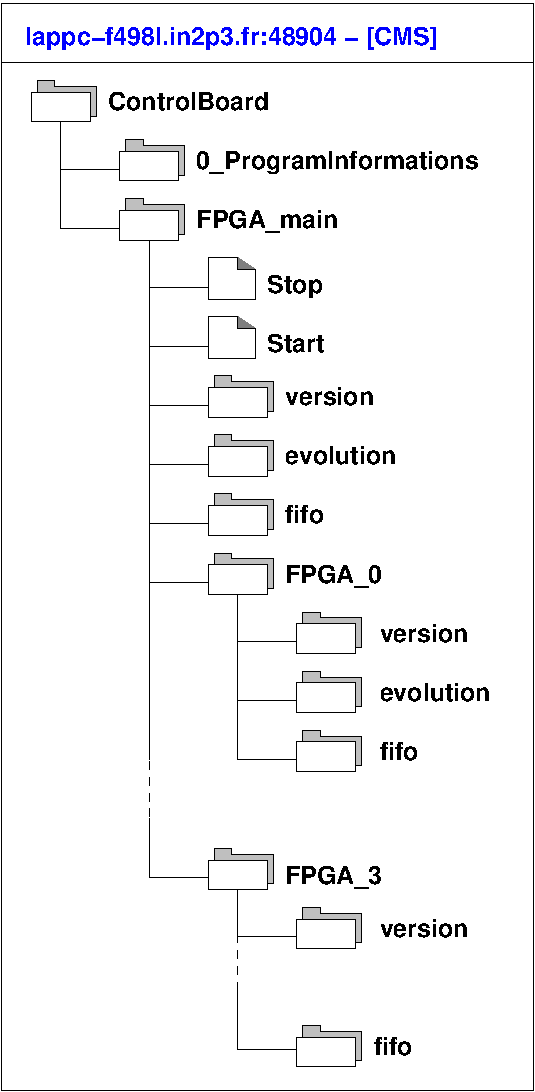
\includegraphics[width=5cm]{appendix/images/MOS_device_example_1.pdf}
\end{center}
\caption{Example of a  device managed through a MOS  server.  The root
  device is named \texttt{ControlBoard}.  First level daughter devices
  are  \texttt{0\_ProgramInformations} and  \texttt{FPGA\_main}.  Here
  the          MOS/OPCUA          server          is          labelled
  \texttt{CMS}.}\label{fig:an:mos_dev_1}
\end{figure}

% TODO


\subsection{Integration of a new device in the Vire environment}

The Vire  API also implements a  mechanism to describe a  hierarchy of
devices.  This  mechanism is independant  of the  one used in  the MOS
system but can  be easily made compatible with it.   This means that a
MOS  hierarchy  of devices  can  be  represented  in Vire.   The  Vire
hierarchy of  devices can  be considered as  some kind  of filesystem,
each device  being a folder with  its unique path, as  shown on figure
\ref{fig:an:mos_dev_2}.   The \emph{methods}  associated to  a devices
(or a datapoint) can be considered as plain executable files stored in
the  device's folder  : they  constitute the  set of  \emph{resources}
associated to the device.


\begin{figure}[h]
\begin{center}
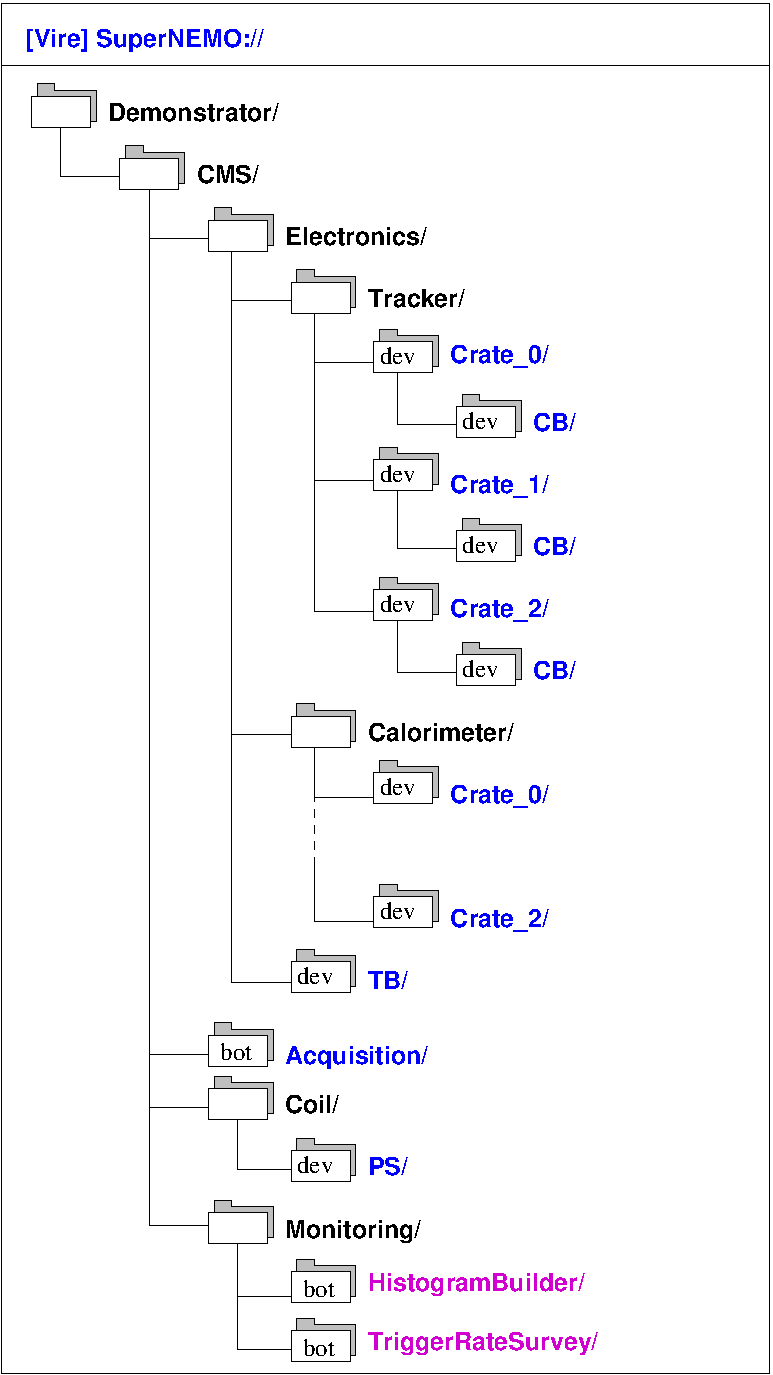
\includegraphics[width=5cm]{appendix/images/MOS_device_example_2.pdf}
\end{center}
\caption{Example of a hierarchy of  devices described by the Vire API.
  The root device is named  \texttt{SuperNEMO:}.  The top level (root)
  device  is  named  \texttt{Demonstrator}.  The  devices  colored  in
  \textcolor{blue}{blue}  are managed  through MOS/OPCUA.  The devices
  colored in \textcolor{magenta}{magenta} are directly embedded in the
  Vire server.  Devices with the \texttt{dev} tag are typical hardware
  device.  Devices  with the  \texttt{bot}  tag  are typical  software
  devices.   The  devices  colored in  \textbf{black}  are  structural
  pseudo-devices used to organize and  present a comprehensive view of
  the hierarchy. }\label{fig:an:mos_dev_2}
\end{figure}

The organisation of this hierarchy of devices is arbitrary and defined
by the designer of the  \emph{Control and Monitoring System}.  What is
important  to  understand  is  that  some  of  these  devices  can  be
associated  to  \emph{hardware  devices}  (a  power  supply  crate,  a
temperature probe\dots) and others  can be \emph{pseudo-devices}, i.e.
pure   software  object   (a   monitoring  robot,   a  file   transfer
daemon\dots).

In the context of the coupling of  the Vire server and the CMS server,
we are  in the event that  some devices are managed  by some MOS/OPCUA
servers and others are managed  in the Vire server itself.  Typically,
\emph{hardware devices}  are systematically managed through  the OPCUA
technology.  Vire has a mechanism to integrate such devices in its own
hierarchy.  This mechanism can  be considered like the \emph{mounting}
of   a   remote   filesystem   from  a   local   filesystem.    Figure
\ref{fig:an:mos_dev_0} illustrates  the case of many  hardware devices
-- managed by MOS -- that are integrated in the Vire system.  From the
Vire point of  view, the user does not see  the implementation details
for such  devices. He  does not  know the identity  of the  MOS server
hosting the device. He does not even know if the device is hosted by a
MOS server.  Devices are simply visible through the standard hierarchy
published by Vire with its  own device naming scheme, regardless their
true location.



\begin{figure}[h]
\begin{center}
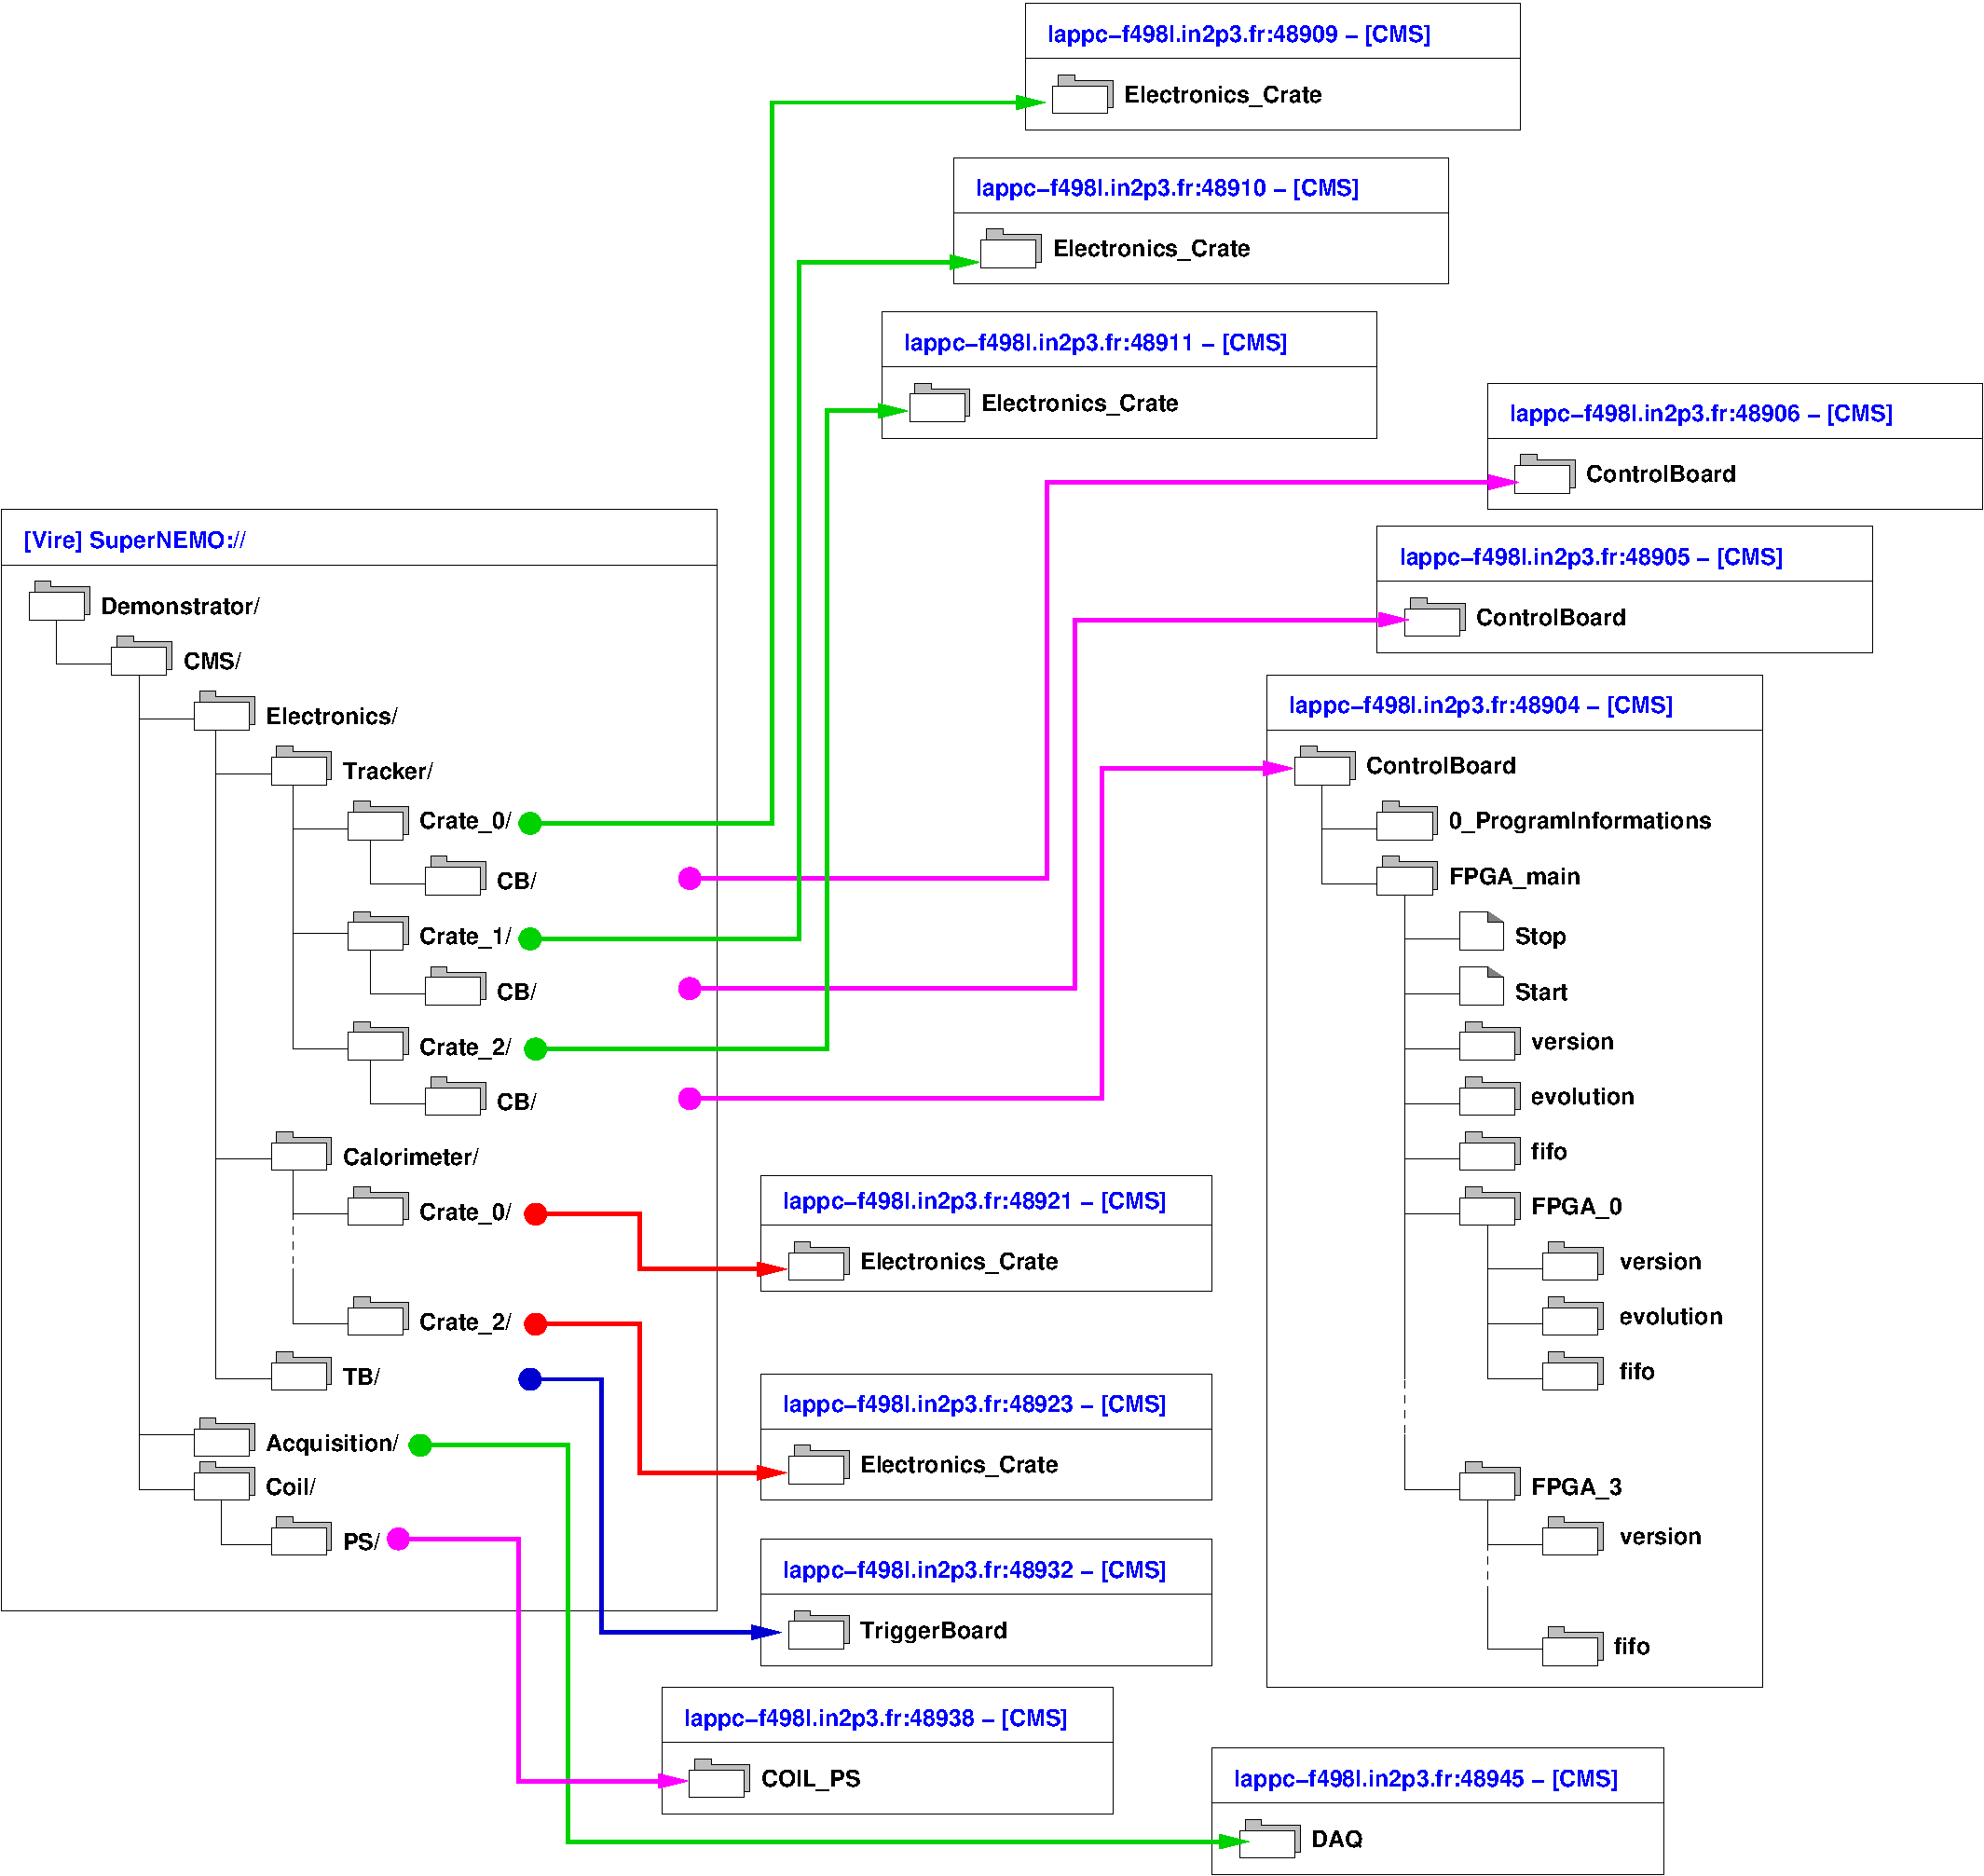
\includegraphics[width=\linewidth]{appendix/images/MOS_device_example_0.pdf}
\end{center}
\caption{The  mounting of  many  MOS device  hierarchies  in the  Vire
  device hierarchy.  Each OPCUA server  runs a simple  hardware device
  that is \emph{mounted} from a specific node with its own path.
%% of  devices described by the Vire API.
%%   The root device is named  \texttt{SuperNEMO:}.  The top level (root)
%%   device is  named \texttt{Demonstrator}. The devices  colored in blue
%%   are managed  through MOS/OPCUA. The  devices colored in  magenta are
%%   directly embedded in the Vire server.  Devices with the \texttt{dev}
%%   tag are typical  hardware device. Devices with  the \texttt{bot} tag
%%   are typical software devices.
}\label{fig:an:mos_dev_0}
\end{figure}




\subsection{Example}

Using  the examples  displayed  in  figure \ref{fig:an:mos_dev_0},  we
consider  in detail  the way  one specific  device managed  by MOS  is
mounted   in  the   Vire   hierarchy.  Figure   \ref{fig:an:mos_dev_3}
illustrates the mounting of a MOS device in Vire.

Here the Vire  server publishes the path of a  device representing the
control board  of the third  electronic crate  for the tracker  of the
SuperNEMO demonstrator module.  The full Vire path of this device is:

\textcolor{blue}{\texttt{SuperNEMO://Demonstrator/CMS/Electronics/Tracker/Crate\_2/CB}}

This is  the only Vire identifier  recognized by user to  address this
device.

On    the   figure,    one    can   see    that    the   MOS    server
\texttt{lappc−f498l.in2p3.fr} (port 48904) hosts a simple device which
is locally named \texttt{ControlBoard}.

When  mounting   this  device  in   the  Vire  hierarchy,   the  local
\texttt{[CMS]}  namespace and  \texttt{ControlBoard} device  names are
hidden and replaced by the Vire device path.  All daughter devices and
datapoints of  the \texttt{CMS/ControlBoard} device are  integrated as
daughters        of        the         Vire        device        named\\
\texttt{SuperNEMO://Demonstrator/CMS/Electronics/Tracker/Crate\_2/CB}.


For example, the \texttt{FPGA\_main} daughter device is now associated
to the following Vire path:

\textcolor{blue}{\texttt{SuperNEMO://Demonstrator/CMS/Electronics/Tracker/Crate\_2/CB/FPGA\_main/}}

and  its  \texttt{Stop} method  is  automatically  addressed with  the
following \emph{leaf} path:

\textcolor{blue}{\texttt{SuperNEMO://Demonstrator/CMS/Electronics/Tracker/Crate\_2/CB/FPGA\_main/Stop}}


\begin{figure}[h]
\begin{center}
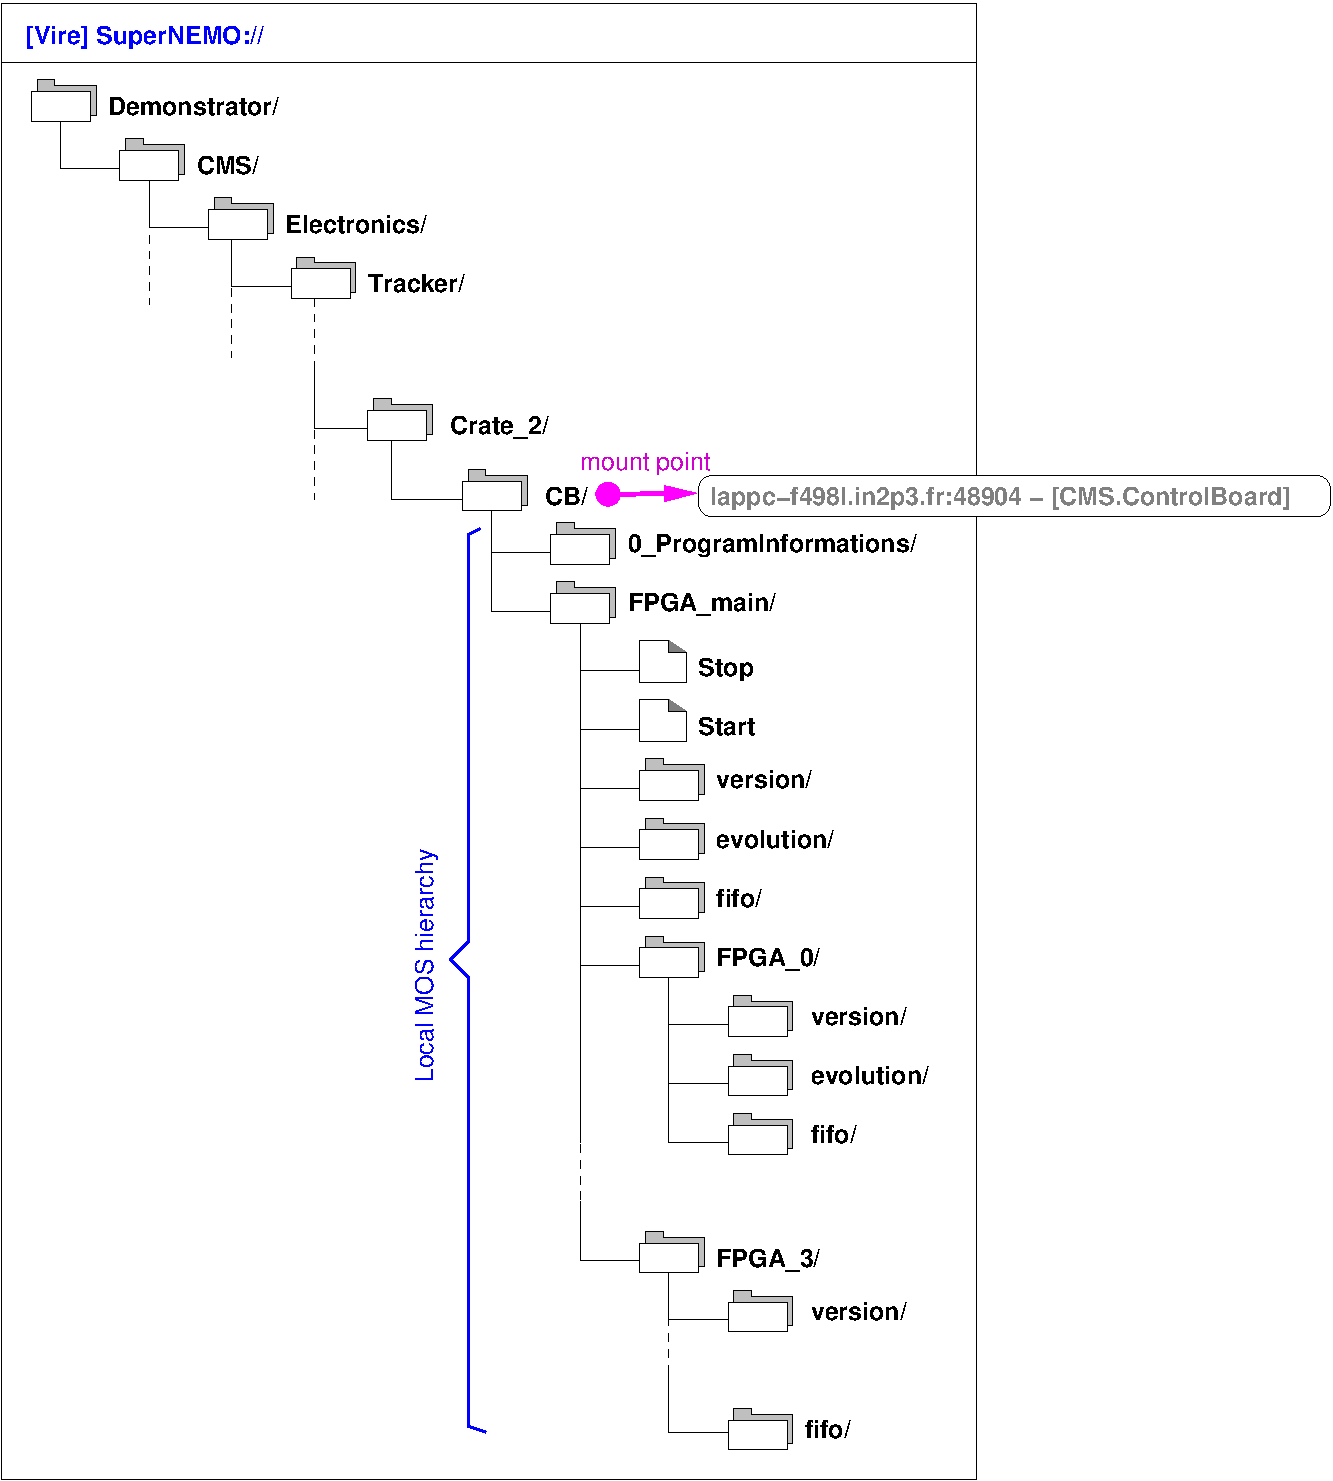
\includegraphics[width=0.8\linewidth]{appendix/images/MOS_device_example_3.pdf}
\end{center}
\caption{The  mounting of  one  MOS device and its local hierarchy  in the  Vire
  device hierarchy.}\label{fig:an:mos_dev_3}
\end{figure}



\subsection{Vire/MOS mapping}

As it can be  seen in the above example, the integration  of a new MOS
device in the Vire system is  achieved through soem kind of filesystem
mounting operation.   Particularly, it is  shown that the MOS  name of
the   mounted  root   device  is   replaced  by   an  arbitrary   Vire
path. However, all daughter  nodes (devices, datapoints) attached from
this root  node have their  relative MOS  names preserved in  the Vire
naming scheme.

Any  resource  (method)  associated  to any  of  such  daughter  nodes
inherits this relative naming scheme.

As Vire applications  describe resources through their  Vire paths, it
is thus needed to build an explicit map that associates resource paths
to MOS address  and name. The CMS  server will be able  to resolve the
MOS server/port and  embedded device associated to  the resource path.

The goal of the \texttt{devices\_launch.conf} file is not only to tell
the CMS server what MOS server should  be loaded and ran at start, but
also  to describe  the  \emph{mounting point/names}  used  by Vire  to
access the resources associated to MOS devices.  From the informations
stored in the  file, an explicit associative array must  be built when
the Vire server connect to the CMS server.  It will play the role of a
resource path resolver  when requests about resources will  be sent by
Vire applications.  This associative array  must be locked  during the
Vire/CMS connection.



%\subsubsection{Preparation of XML device models}

%% \noindent\underline{Pre-condition:}
%% The device is working and validated through the MOS/OPCUA server

%% \begin{enumerate}

%% \item Produce XML décrivant le modèle du device enrichi
%%   des metadata
%% Rédaction du fichier XML décrivant le modèle du device

%% \item Génération des fichiers model du type de device pour Vire

%% \item Génération des fichiers instances resolv.conf

%% \end{enumerate}


\vfill
\pagebreak
\clearpage

% end


\section{Vire messages}\label{app:vire_messages}

Within Vire  and between Vire  components and external  components, we
use  a communication  system  based on  Vire  messages.  This  section
describes the structure of such messages.

\subsection{General structure of a message}

Each message consists in two parts (figure \ref{fig-vire-message-message-cpp}):
\begin{itemize}

\item  the  \emph{header}  is   dedicated  to  generic  and  typicalle
  mandatory  informations  which  document   the  message  itself  and
  arbitrary high-level metadata.

\item  the \emph{body}  of the  message  contains the  real data: the payload.
  The structure of the message body depends on some convention. Vire uses
  its own convention to embed the payload data.

\end{itemize}

\begin{figure}[h]
\vskip 10pt
\small
\begin{Verbatim}[frame=single,xleftmargin=0.cm,label=\fbox{C++}]
struct vire::message::message {
  message_header header; // Header of the message
  message_body   body;   // Body of the message
};
\end{Verbatim}
\normalsize
\caption{The structure of a Vire message object (C++  class:
  \texttt{"vire::message::message"})}\label{fig-vire-message-message-cpp}
\end{figure}

\subsection{The message header}

The header contains (figure \ref{fig-vire-message-message_header-cpp}):
\begin{itemize}

  \item The mandatory \texttt{message\_id}  attribute is an identifier
    of the  message which  document the emitter  and a  unique message
    number.   Each emitter  is  responsible of  the  numbering of  the
    messages it  emits, typically using an  incremental technique. The
    message  number is  a positive  integer, starting  from 0  (figure
    \ref{fig-vire-message-message_identifier-cpp}).

  \item  The \texttt{timestamp}  attribute  encodes the  approximative
    time point when the message was  created. It contains the date and
    the time, using at least microsecond resolution.

    Typically,  with  JSON  encoding  system, it  is  expected  to  be
    formatted as a character string, using the following ISO format:

    \begin{center}
      \texttt{yyyymmddThhmmss.uuuuuu}
    \end{center}

    \noindent where:

    \vskip -10pt
    \begin{itemize}
    \item[\texttt{yyyymmdd} :] encodes year/month/day,
    \item[\texttt{hhmmssd} :] encodes hour/minute/second,
    \item[\texttt{uuuuuu} :] encodes microseconds.
    \end{itemize}

  \item   In   the   case    of   a   \emph{response}   message,   the
    \texttt{in\_reply\_to} attribute is set to identify the associated
    request message.

  \item  The \texttt{asynchronous}  boolean  attribute is  set if  the
    message processing  is explicitely requested  by the source  to be
    asynchronous (non-blocking).  In  RPC transactions, where requests
    are transmitted from one point to  the other, its default value is
    \emph{false}.   It  is possible  to  force  a RPC  transaction  in
    asynchronous mode.   This use  case is documented  elsewhere.  For
    event messaging, this flag is conventionally set to \emph{true}.

  \item  The  \texttt{body\_layout\_id}  attribute  is  the  mandatory
    identifier   of   the   layout   of  the   message   body   (class
    \texttt{"vire::utility::model\_identifier"}).  The  default layout
    for     message     body     inside    the     Vire     API     is
    \texttt{"vire::message::body\_format::typed\_payload"}, with version
    \texttt{"1.0"}                                             (figure
    \ref{fig-vire-utility-model_identifier-cpp}).

\end{itemize}


\begin{figure}[h]
\vskip 10pt
\small
\begin{Verbatim}[frame=single,xleftmargin=0.cm,label=\fbox{C++}]
struct vire::message::message_header {
  message_identifier message_id;     // Message identifier from the emitter.
  std::string        timestamp;      // Timestamp.
  message_identifier in_reply_to;    // Message identifier of the associated
                                     // request message (optional).
  bool               asynchronous,   // Asynchronous flag.
  vire::utility::model_identifier     body_layout_id; // Body layout identifier.
  std::map<std::string, std::string>  metadata;       // Key/value metadata dictionary.
};
\end{Verbatim}
\normalsize
\caption{The  structure  of  a   message  header  object  (C++  class:
  \texttt{"vire::message::message\_header"}).}\label{fig-vire-message-message_header-cpp}
\end{figure}

\begin{figure}[h]
\vskip 10pt
\small
\begin{Verbatim}[frame=single,xleftmargin=0.cm,label=\fbox{C++}]
struct vire::message::message_identifier {
  std::string emitter; // Name identifying the emitter of the message.
  int32_t     number;  // Number identifying the message in the emitter's
                       // message numbering scheme.
};
\end{Verbatim}
\normalsize
\caption{The      structure      of     a      message      identifier
  (C++  class:  \texttt{"vire::message::message\_identifier"}).}
\label{fig-vire-message-message_identifier-cpp}
\end{figure}

\begin{figure}[h]
\vskip 10pt
\small
\begin{Verbatim}[frame=single,xleftmargin=0.cm,label=\fbox{C++}]
struct vire::utility::model_identifier {
  std::string name;    // Name identifying the format of the message.
  std::string version; // String identifying the version of the format.
};
\end{Verbatim}
\normalsize
\caption{The structure of a model identifier (C++  class:  \texttt{"vire::utility::model\_identifier"}.}\label{fig-vire-utility-model_identifier-cpp}
\end{figure}




\begin{figure}[h]
\vskip 10pt
\small
\begin{Verbatim}[frame=single,xleftmargin=0.cm,label=\fbox{JSON}]
{
   "header" : {
      "message_id" : {
         "emitter" : "vire.server",
         "number" : 42
      },
      "timestamp" : "20160930T141408.413443",
      "in_reply_to" : {
         "initialized" : true,
         "value" : {
            "emitter" : "vire.client.0",
            "number" : 23
         }
      },
      "asynchronous" : false,
      "body_layout_id" : {
         "name" : "vire::message::body_format::typed_payload",
         "version" : {
            "initialized" : true,
            "value" : "1.0"
         }
      },
      "metadata" : [
         {
            "key" : "key1",
            "value" : "foo"
         },
         {
            "key" : "key2",
            "value" : "42"
         },
         {
            "key" : "key3",
            "value" : "3.1415899999999999"
         },
         {
            "key" : "key4",
            "value" : "true"
         }
      ]
   }
  "body" : {
      ...
   }
}
\end{Verbatim}
\normalsize
\caption{Example of  a   message  header  object in JSON format.}
\label{fig-vire-message-message_header-json}
\end{figure}

\vfill
\clearpage
\pagebreak

\subsection{The message body}

The    default    message   body    layout    in    Vire   is    named
\texttt{"vire::message::body\_format::typed\_payload"}        (version
\texttt{"1.0"}).   Each  message used  within  the  Vire framework  is
supposed to use this layout.  The general idea is that the body of the
message embeded the  \emph{payload object} that has  to be transmitted
between  two components  of  the system.   \emph{Payload objects}  are
classified in one of the three following categories:

\begin{enumerate}

\item \emph{Request}:  describes a request submitted  by one component
  to another component (generally during a synchronous RPC transaction).

\item  \emph{Response}: describes  the  response to  a former  request
  (generally during a synchronous RPC transaction).

\item \emph{Event}: describes an  arbitrary information record (alarm,
  exception, signal\dots) which is transmitted asynchronously.

\end{enumerate}

Vire implements the following class hierarchy:

\begin{center}
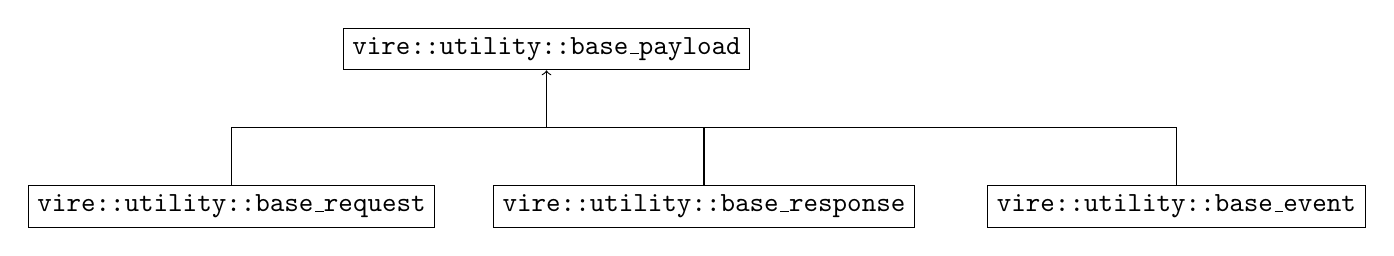
\begin{tikzpicture}
  \node (payload)  at (0,2)  [draw] {\texttt{vire::utility::base\_payload}};
  \node (request)  at (-4,0) [draw] {\texttt{vire::utility::base\_request}};
  \node (response) at (2,0)  [draw] {\texttt{vire::utility::base\_response}};
  \node (event)    at (8,0)  [draw] {\texttt{vire::utility::base\_event}};

  %\draw[style=help lines] (-3,-1) grid (10,4);
  \draw (node cs:name=response,anchor=north) |- (0,1);
  \draw (node cs:name=event,anchor=north)    |- (0,1);
  \draw[->] (node cs:name=request,anchor=north)
  |- (0,1) -| (node cs:name=payload,anchor=south);
\end{tikzpicture}
\end{center}

The requirements for the transmitted object are the following:

\begin{itemize}

\item The  type of the object  must be conventionally associated  to a
  unique     \emph{model      identifier}     object      (see     the
  \texttt{"vire::utility::model\_identifier"} class)  which contains a
  unique   name   (\textit{string    identifier})   and   possibly   a
  \textit{version identifier}.  Each software  component that may send
  or  receive the  object  should agree  on  this type  identification
  scheme.   This   enable  the  use  of   object  factories,  whatever
  programming  langage  is used  on  both  side of  the  communication
  system.

\item  For each  software component,  the object  type must  have some
  dedicated  encoding/decoding  functions  available  (again  whatever
  programming language is used). For example the Vire API supports the
  following encoding formats:

  \begin{itemize}

  \item JSON (MIME  encoding type: \texttt{"application/x-json"}), which
    is supportable by many languages,

  \item  Protobuf  (Google  Protocol   Buffers,  MIME  encoding  type:
    \texttt{"application/x-protobuf"}), which is also widely supported,

  \item   Boost/serialisation   (XML,    text   or   binary   archives
    \texttt{"application/x-boost-serialization-xml"},
    \texttt{"application/x-boost-serialization-text"},
    \texttt{"application/x-boost-serialization-binary"}),    which    in
    principle is supported by C++ only.

  \end{itemize}

  The Protobuf  encoding format will be  used to serialize/deserialize
  the  Vire  messages transported  between  the  Vire server  and  the
  CMS/LAPP server.

\end{itemize}

Vire uses a dedicated layout to represent the body of any message with
its embedded payload object. With this technique, the structure of the
body          contains         two          attributes         (figure
\ref{fig-app-vire-message-message_body-cpp}):

\begin{enumerate}

\item The \texttt{payload\_type\_id} specifies the type of the payload
  object   (figure   \ref{fig-app-vire-utility-model_identifier-cpp}).
  This unique name  is conventionaly fixed for a  given application. A
  version tag allows to support possible evolution of the object type.

\item The  \texttt{payload} is a  handle to  a payload object  of type
  request, response or event.

  %% \begin{itemize}
  %% \item Within  the producer  component of  the message,  the encoding
  %%   function associated to the object  type is responsible to generate
  %%   the JSON stream for the object and store it in the buffer.

  %% \item Within  the consumer  component of  the message,  the decoding
  %%   function associated to the object type is responsible to parse the
  %%   JSON stream stored in the buffer and restore the object in memory.

  %% \end{itemize}

  It is expected  that, on both sides of the  connection, the software
  components can  access dedicated  software plugins which  ensure the
  support  of  various   \emph{payload  object  types}  conventionnaly
  associated  with  their  \emph{payload type  identifiers}  and  also
  providing JSON and/or Protobuf encoding/decoding functionalities.

  %% The   system  allows  to  support
  %% modification  in the  structure of  the objects  thanks to  version
  %% tagging.

\end{enumerate}

\begin{figure}[h]
\vskip 10pt
\small
\begin{Verbatim}[frame=single,xleftmargin=0.cm,label=\fbox{C++}]
struct message_body {
  vire::utility::model_identifier     payload_type_id; // Object type identifier.
  const vire::utility::base_payload * payload;         // Handle to a payload object.
};
\end{Verbatim}
\normalsize
\caption{The structure of a message body object (C++).}
\label{fig-app-vire-message-message_body-cpp}
\end{figure}

\begin{figure}[h]
\vskip 10pt
\small
\begin{Verbatim}[frame=single,xleftmargin=0.cm,label=\fbox{JSON}]
{
  "header" : {
    ...
  },
  "body" : {
    "payload_type_id" : {
      "name" : "vire::message::testing::error_event",
      "version" : {
        "initialized" : false
      }
    },
    "payload" : {
      "timestamp" : "20160930T141743.759085"
      "err" : {
        "code" : 3,
        "message" : "A basic error"
      },
    }
  }
}
\end{Verbatim}
\normalsize
\caption{Example of  a   message  body  object in JSON format.}
\label{fig-vire-message-message_body-json}
\end{figure}

\vfill
\clearpage
\pagebreak

% end

%\input{appendix/app_json_fmt.tex}

\section{The \emph{Protocol Buffers} format}\label{app:protobuf_fmt}

\subsection{Introduction}

The  Google  Protocol Buffers  (\emph{protobuf})  library  is used  to
represent the objects that are exchanged between the Vire clients, the
Vire server and the CMS server.  The  version 3 of the format is used,
implying   at   least   version   3.0.0  (September   2016)   of   the
\emph{protobuf} library.

Each  data   structure  of  interest   can  be  described   through  a
\texttt{.proto}  file  from  which  stub files  can  be  automatically
generated  with the  \texttt{protoc} compiler.  For Vire  and its  CMS
interface, the C++ and Java programming languages will be used.


A  collection of  \texttt{.proto}  files are  provided  with the  Vire
library to represent all kind  of data structures transferable between
networked agents  (Vire server,  Vire clients, CMS/LAPP  server).  The
objects of  the highest level  are named \emph{payload  objects} (like
\emph{request},  \emph{response} and  \emph{event} objects).   They
are composed of attributes of more basic data structures.

\subsection{Example}

The following  class diagram  illustrates two data  structures defined
within the Vire library with an inheritance relationship between them.

\begin{center}
  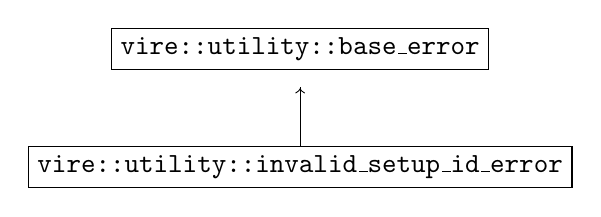
\begin{tikzpicture}
    \node (base)     at (0,1.5)  [draw] {\texttt{vire::utility::base\_error}};
    \node (setup)    at (0,0)  [draw] {\texttt{vire::utility::invalid\_setup\_id\_error}};

    \draw[->]   (node cs:name=setup,anchor=north) |- (0,1);
    |- (0,1) -| (node cs:name=base,anchor=south);
  \end{tikzpicture}
\end{center}

The \texttt{vire::utility::base\_error}  is the  parent class  for all
\emph{error}  objects.   It  contains   two  attributes:   an  integer
\emph{error code}  and a  character string describing  the \emph{error
  message}.

The   \texttt{vire::utility::invalid\_setup\_id\_error}  class   is  a
specialized error class  which represents explicitely an  error due to
an identification  failure of  the experimental setup.   It implements
additional mutually exclusive attributes: the \emph{unrecognized name}
of the setup or the \emph{unrecognized version} of the setup.

This   example  illustrates   the  protobuf   representation  of   the
\texttt{vire::utility::base\_error}  in the  Vire  library, using  the
\texttt{"vire/utility/BaseError.proto"} file:

\small
\begin{Verbatim}[frame=single,xleftmargin=0.cm,label=\fbox{protobuf}]
  syntax = "proto3";
  package vire.utility; // Namespace

  message BaseError {

    // reserved 1; // Reserved for _base message

    // Attributes:
    int32  code           = 100; // The error code
    string message_format = 101; // The error description message

  }
\end{Verbatim}
\normalsize

\vfill
\clearpage
\pagebreak

\subsection{Vire protobuf conventions}

Vire uses the following conventions:

\begin{enumerate}

\item
  The member index  \texttt{1} is reserved to represent the  link of a
  class to its main base/parent class (if any).  It is not used if the
  data structure does not inherit any data structure.
  If a data structure naturally inherits another one, it is thus possible
  to  represent the  inheritance  relationship as  illustrated with  the
  \texttt{"vire/utility/InvalidSetupIdError.proto"}      file      which
  represents the \texttt{vire::utility::invalid\_setup\_id\_error} class
  in the Vire library:

  \small
  \begin{Verbatim}[frame=single,xleftmargin=0.cm,label=\fbox{protobuf}]
    syntax = "proto3";
    package vire.utility; // Namespace

    import "vire/utility/BaseError.proto"; // Dependency

    message InvalidSetupIdError {

      BaseError _base = 1; // The base class

      // Additional attributes:
      oneof detail { // Mutual exclusion
        string invalid_setup_name    = 100; // The failed setup name
        string invalid_setup_version = 101; // The failed setup version
      }

    }
  \end{Verbatim}
  \normalsize

\item The  \texttt{\_base} member  is conventionally  used to  represent the
  inheritance   relationship    from   a   data   structure    of   type
  \texttt{"vire.utility.BaseError"}.

\item Member indexes from \texttt{2}  to \texttt{99} are also reserved
  for possible future usage (multiple inheritance, metadata\dots).

\item
  The first member of the data structure must start at index \texttt{100}.

\end{enumerate}

\vfill
\clearpage
\pagebreak

% end


\section{Vire payload objects}\label{app:payload}

\subsection{Introduction}

As  mentioned in  appendix \ref{app:protobuf_fmt},  Vire messages  are
wrappers for \emph{payload objects}.  Each  type of payload object can
be represented  through the \emph{protobuf} mechanism.   The following
class hierarchy shows the base architecture used to define new payload
objects.

\begin{center}
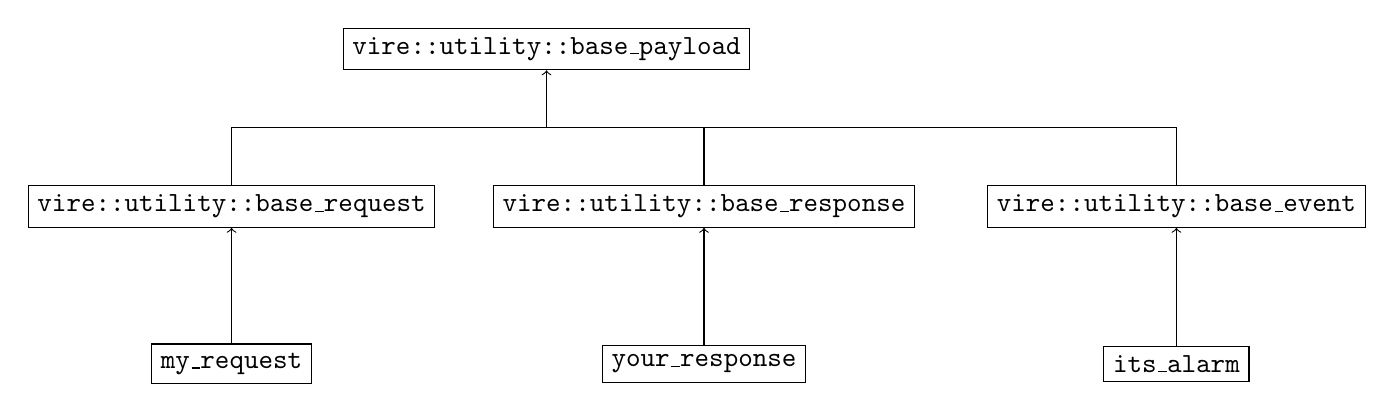
\begin{tikzpicture}
  \node (payload)  at (0,2)   [draw] {\texttt{vire::utility::base\_payload}};
  \node (request)  at (-4,0)  [draw] {\texttt{vire::utility::base\_request}};
  \node (response) at (2,0)   [draw] {\texttt{vire::utility::base\_response}};
  \node (event)    at (8,0)   [draw] {\texttt{vire::utility::base\_event}};
  \node (my)       at (-4,-2) [draw] {\texttt{my\_request}};
  \node (your)     at (2,-2)  [draw] {\texttt{your\_response}};
  \node (its)    at (8,-2)    [draw] {\texttt{its\_alarm}};

  %\draw[style=help lines] (-6,-2) grid (10,2);
  \draw (node cs:name=response,anchor=north) |- (0,1);
  \draw (node cs:name=event,anchor=north)    |- (0,1);
  \draw[->] (node cs:name=request,anchor=north)
  |- (0,1) -| (node cs:name=payload,anchor=south);
  \draw[->] (node cs:name=my,anchor=north)
  |- (-4,-1) -| (node cs:name=request,anchor=south);
  \draw[->] (node cs:name=your,anchor=north)
  |- (2,-1) -| (node cs:name=response,anchor=south);
  \draw[->] (node cs:name=its,anchor=north)
  |- (8,-1) -| (node cs:name=event,anchor=south);
\end{tikzpicture}
\end{center}


\begin{center}
\vskip 10pt
\small
\begin{tabular}{|l|l|l|}
  \hline
  \textbf{Vire C++ class} & \textbf{protobuf message type} & \textbf{protobuf definition file} \\
  \hline
  \hline
  \multicolumn{3}{|c|}{\emph{general types}} \\
  \hline
  boost::posix\_time::ptime & google.protobuf.Timestamp & google/protobuf/timestamp.proto \\
  \hline
  \hline
  \multicolumn{3}{|c|}{\emph{identifier types}} \\
  \hline
  vire::utility::base\_identifier & vire.utility.Baseidentifier & vire/utility/Baseidentifier.proto \\
  \hline
  vire::utility::instance\_identifier & vire.utility.InstanceIdentifier & vire/utility/InstanceIdentifier.proto \\
  \hline
  vire::utility::model\_identifier & vire.utility.ModelIdentifier & vire/utility/ModelIdentifier.proto \\
  \hline
  \hline
  \multicolumn{3}{|c|}{\emph{error types}} \\
  \hline
  vire::utility::base\_error & vire.utility.BaseError & vire/utility/BaseError.proto \\
  \hline
  vire::utility::invalid\_context\_error & vire.utility.InvalidContextError & vire/utility/InvalidContextError.proto \\
  \hline
  vire::utility::invalid\_setup\_id\_error & vire.utility.InvalidSetupIdError & vire/utility/InvalidSetupIdError.proto \\
  \hline
  \hline
  \multicolumn{3}{|c|}{\emph{payload types}} \\
  \hline
  vire::utility::base\_payload & vire.utility.BasePayload & vire/utility/BasePayload.proto \\
  \hline
  vire::utility::base\_request & vire.utility.BaseRequest & vire/utility/BaseRequest.proto \\
  \hline
  vire::utility::base\_response & vire.utility.BaseResponse & vire/utility/BaseResponse.proto \\
  \hline
  vire::utility::base\_event & vire.utility.BaseEvent & vire/utility/BaseEvent.proto \\
  \hline
  vire::utility::base\_alarm & vire.utility.BaseAlarm & vire/utility/BaseAlarm.proto \\
  \hline
  \hline
  \multicolumn{3}{|c|}{\emph{messenging types}} \\
  \hline
  vire::message::message\_identifier & vire.message.MessageIdentifier & vire/message/MessageIdentifier.proto \\
  \hline
  vire::message::msg\_header & vire.message.MsgHeader & vire/message/MsgHeader.proto \\
  \hline
  vire::message::msg\_body & vire.message.MsgBody & vire/message/MsgBody.proto \\
  \hline
  vire::message::message & vire.message.Message & vire/message/Message.proto \\
  \hline
\end{tabular}
\normalsize
\end{center}


\begin{center}
\vskip 10pt
\small
\begin{tabular}{|l|l|l|}
  \hline
  \multicolumn{3}{|c|}{\emph{Resource management related types}} \\
  \hline
  vire::cms::resource\_status\_record & vire.cms.ResourceStatusRecord & vire/cms/ResourceStatusRecord.proto \\
  \hline
  vire::cms::resource\_fetch\_status\_request & vire.cms.ResourceFetchStatusRequest & vire/cms/ResourceFetchStatusRequest.proto \\
  \hline
  vire::cms::resource\_fetch\_status\_success\_response & vire.cms.ResourceFetchStatusSuccessResponse & vire/cms/ResourceFetchStatusSuccessResponse.proto \\
  \hline
  vire::cms::resource\_fetch\_status\_failure\_response & vire.cms.ResourceFetchStatusFailureResponse & vire/cms/ResourceFetchStatusFailureResponse.proto \\
  \hline
  vire::cms::resource\_exec\_request & vire.cms.ResourceExecRequest & vire/cms/ResourceExecRequest.proto \\
  \hline
  vire::cms::resource\_exec\_success\_response & vire.cms.ResourceExecSuccessResponse & vire/cms/ResourceExecSuccessResponse.proto \\
  \hline
  vire::cms::resource\_exec\_failure\_response & vire.cms.ResourceExecFailureResponse & vire/cms/ResourceExecFailureResponse.proto \\
  \hline
  vire::cms::resource\_exec\_non\_blocking\_request & vire.cms.ResourceExecNonBlockingRequest & vire/cms/ResourceExecNonBlockingRequest.proto \\
  \hline
  vire::cms::resource\_exec\_non\_blocking\_ack\_response & vire.cms.ResourceExecNonBlockingAckResponse & vire/cms/ResourceExecNonBlockingAckResponse.proto \\
  \hline
  vire::cms::resource\_exec\_non\_blocking\_noack\_response & vire.cms.ResourceExecNonBlockingNoackResponse & vire/cms/ResourceExecNonBlockingNoackResponse.proto \\
  \hline
  vire::cms::resource\_exec\_non\_blocking\_success\_event & vire.cms.ResourceExecNonBlockingSuccessEvent & vire/cms/ResourceExecNonBlockingSuccessEvent.proto \\
  \hline
  vire::cms::resource\_exec\_non\_blocking\_failure\_event & vire.cms.ResourceExecNonBlockingFailureEvent & vire/cms/ResourceExecNonBlockingFailureEvent.proto \\
  \hline
  vire::cms::resource\_exec\_error & vire.cms.ResourceExecError & vire/cms/ResourceExecError.proto \\
  \hline
  vire::cms::invalid\_status\_error & vire.cms.ResourceExecError & vire/cms/ResourceExecError.proto \\
  \hline
  %% vire::cms::invalid\_credentials\_error & vire.cms.InvalidCredentialsError & vire/cms/InvalidCredentialsError.proto \\
  %% \hline
  %% vire::cms::invalid\_user\_error & vire.cms.InvalidUserError & vire/cms/InvalidUserError.proto \\
  %% \hline
  vire::cms::invalid\_resource\_error & vire.cms.InvalidUserError & vire/cms/InvalidUserError.proto \\
  \hline
  vire::cms::no\_pubsub\_resource\_error & vire.cms.NoPubsubResourceError & vire/cms/NoPubsubResourceError.proto \\
  \hline
  \hline
  \multicolumn{3}{|c|}{\emph{Resource pub/sub management types}} \\
  \hline
  vire::cms::resource\_pubsub\_subscribe\_request & vire.cms.ResourcePubsubSubscribeRequest & vire/cms/ResourcePubsubSubscribeRequest.proto \\
  \hline
  vire::cms::resource\_pubsub\_subscribe\_success\_response & vire.cms.ResourcePubsubSubscribeRSuccessResponse & vire/cms/ResourcePubsubSubscribeRSuccessResponse.proto \\
  \hline
  vire::cms::resource\_pubsub\_subscribe\_failure\_response & vire.cms.ResourcePubsubSubscribeRFailureResponse & vire/cms/ResourcePubsubSubscribeRSuccessResponse.proto \\
  \hline
  \hline
  \multicolumn{3}{|c|}{\emph{Vire/CMS server interface types}} \\
  \hline
  vire::cmsinterface::connection\_request & vire.cmsinterface.ConnectionRequest & vire/cmsinterface/ConnectionRequest.proto \\
  \hline
  vire::cmsinterface::connection\_success\_response & vire.cmsinterface.ConnectionSuccessResponse & vire/cmsinterface/ConnectionSuccessResponse.proto \\
  \hline
  vire::cmsinterface::connection\_failure\_response & vire.cmsinterface.ConnectionFailureResponse & vire/cmsinterface/ConnectionFailureResponse.proto \\
  \emph{embedded:} unknown\_resources\_error & .UnknownResourcesError &  \\
  \hline
  vire::cmsinterface::disconnection\_request & vire.cmsinterface.DisconnectionRequest & vire/cmsinterface/DisconnectionRequest.proto \\
  \hline
  vire::cmsinterface::disconnection\_success\_response & vire.cmsinterface.DisconnectionSuccessResponse & vire/cmsinterface/DisconnectionSuccessResponse.proto \\
  \hline
  %% \hline
  %% vire::cmsinterface::disconnection\_failure\_response & vire.cmsinterface.DisconnectionFailureResponse & vire/cmsinterface/DisconnectionFailureResponse.proto \\
\end{tabular}
\normalsize
\end{center}

\subsection{Basic data structures}

Any  payload object  (request, response  or event)  generally contains
some information records which are  specific to the functionalities of
the  payload  object they  belong.   These  records are  of  arbitrary
types. Of course they should be  translatable in terms of the protobuf
library.
%Of course they can be (de)serialized using JSON.
Some of these types are very  general and defined within the Vire core
API itself because they are reused by various payload objects not only
through  the Vire-CMS/LAPP  interface  but also  between  Vire clients  and
servers, independently  of the  CMS/LAPP server.  However,  the use  of the
Protocol Buffers interface makes possible  to publish the interface of
such data to the outside world, including the CMS/LAPP server in priority.

%% Other one are specific to the Vire/CMS interface and thus managed only
%% in the \texttt{Vire\_CMSInterface} API.
These  types  are considered  as  \emph{basic}.  Among them  we  find:
generic error  types, generic  identifier types,  timestamps, resource
status records\dots We propose to describe them in this section.

Once a sufficient collection of  basic data record types is available,
it  is possible  to describe  high  level payload  object types  which
aggregate attributes of such types.

Other record  types are specific to  some payload objects and  will be
never  used outside  the scope  of these  payload objects.   Such data
structures will be  explicitely declared with the  payload object they
belong to, likely as embedded types/classes.


\subsubsection{Errors}

Some  \emph{response} or  \emph{event} payload  objects may  contain a
specific  error  record  object.   A  \emph{failure  response}  or  an
\emph{exception  event}  object will  generally  embed  such an  error
record object.

Each  \emph{error record}  is represented  by an  instance of  a given
error type.   Each of  the error  types defined  in Vire  inherits the
\texttt{vire::utility::base\_error}      base       class      (figure
\ref{fig-app-payload-base_error})   which   contains   the   following
attributes:

\begin{itemize}

\item the error code: A non zero  integer which is set to 1 by default
  (indicating  a  generic  failure  case).   The  error  code  can  be
  conventionally  set to  any positive  integer value  to represent  a
  specific error case, depending on the context.

\item the error  message: an optional human  readable character string
  which documents the error as usefully as possible.

\end{itemize}

\begin{figure}[h]
\vskip 10pt
\small
\begin{Verbatim}[frame=single,xleftmargin=0.cm,label=\fbox{C++}]
struct vire::utility::base_error
{
  // Attributes:
  int         code;           // Error code (>0).
  std::string message_format; // Error message (optional).
};
\end{Verbatim}
\normalsize
\caption{The structure of a \texttt{"vire::utility::base\_error"} object
  (C++).}
\label{fig-app-payload-base_error}
\end{figure}


%% An example of JSON formatted basic error object is given in figure
%% \ref{fig-app-payload-base_error-1}.
%%
%% \begin{figure}[h]
%% \vskip 10pt
%% \small
%% \begin{Verbatim}[frame=single,xleftmargin=0.cm,label=\fbox{\texttt{JSON}}]
%% {
%%   "code" : "42",
%%   "message_format" : "Invalid AMQP server port=[2341]"
%% }
%% \end{Verbatim}
%% \normalsize
%% \caption{JSON  formatted  basic  error  object  (class
%%   \texttt{vire::utility::base\_error}.}
%% \label{fig-app-payload-base_error-1}
%% \end{figure}

Several type of generic errors are defined in Vire:


\begin{center}
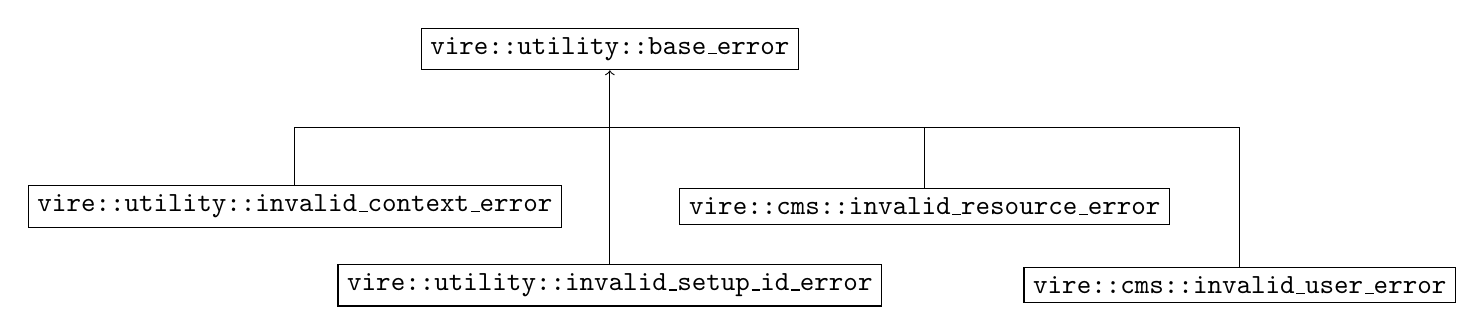
\begin{tikzpicture}
  \node (base)     at (0,2)  [draw] {\texttt{vire::utility::base\_error}};
  \node (context)  at (-4,0) [draw] {\texttt{vire::utility::invalid\_context\_error}};
  \node (setup)    at (0,-1)  [draw] {\texttt{vire::utility::invalid\_setup\_id\_error}};
  \node (resource) at (4,0)  [draw] {\texttt{vire::cms::invalid\_resource\_error}};
  \node (user)     at (8,-1)  [draw] {\texttt{vire::cms::invalid\_user\_error}};

  \draw     (node cs:name=setup,anchor=north)    |- (0,1);
  \draw     (node cs:name=resource,anchor=north) |- (0,1);
  \draw     (node cs:name=user,anchor=north)     |- (0,1);
  \draw[->] (node cs:name=context,anchor=north)
  |- (0,1) -| (node cs:name=base,anchor=south);
\end{tikzpicture}
\end{center}

\noindent
Here are a few error object types defined in Vire.  Some types belongs
to the \texttt{utility} namespace, other  ones are in the \texttt{cms}
namespace:

\begin{itemize}

\item \texttt{"vire::utility::invalid\_context\_error"} : occurs typically when
  the general context of the execution of a given resource is not adapted.\\
  It is mapped to the \texttt{"vire.utility.InvalidContextError"} protobuf record.

\item \texttt{"vire::utility::invalid\_setup\_id\_error"} : occurs in case
  of an invalid identification of the experimental setup managed
  by the Vire or CMS server.\\
  It is mapped to the \texttt{"vire.utility.InvalidSetupIdError"} protobuf record.

\item \texttt{"vire::cms::invalid\_resource\_error"} : occurs in case
  of an invalid identification of a resource.\\
  It is mapped to the  \texttt{"vire.cms.InvalidResourceError"} protobuf record.

\item \texttt{"vire::cms::invalid\_status\_error"}: occurs when an attempt
  to access a resource that has not the proper status.\\
  It is mapped to the  \texttt{"vire.cms.InvalidStatusError"} protobuf record.

\item \texttt{"vire::cms::invalid\_user\_error"} : occurs in case
  of an invalid identification of an user.\\
  It is mapped to the  \texttt{"vire.cms.InvalidUserError"} protobuf record.

\item \texttt{"vire::cms::invalid\_credentials\_error"} : occurs in case
  of user authentication error.\\
  It is mapped to the  \texttt{"vire.cms.InvalidCredentialsError"} protobuf record.

\item \texttt{"vire::cms::resource\_exec\_error"} : occurs in case
  of error at the execution of a given resource.\\
  It is mapped to the  \texttt{"vire.cms.ResourceExecError"} protobuf record.

\end{itemize}



\subsubsection{Object and type identifiers}

Vire  uses  some dedicated  classes  to  represent the  identifier  of
various objects  (or \emph{instances})  as well  as various  types (or
\emph{models})  of components.  Vire  implements  the following  class
hierarchy:

\begin{center}
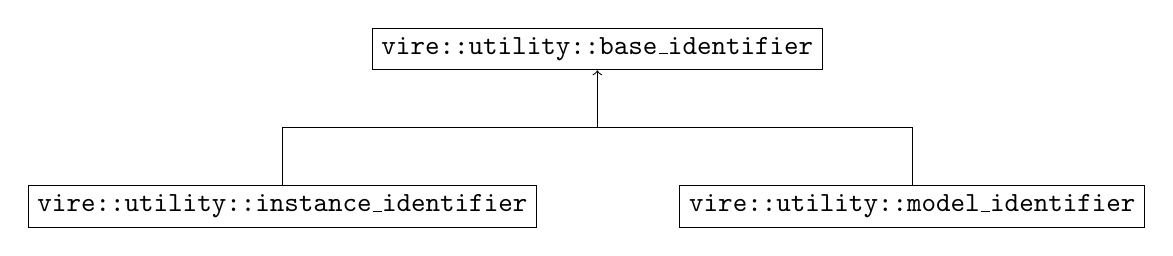
\begin{tikzpicture}
  \node (base)  at (0,2)  [draw] {\texttt{vire::utility::base\_identifier}};
  \node (instance)  at (-4,0) [draw] {\texttt{vire::utility::instance\_identifier}};
  \node (model) at (4,0)  [draw] {\texttt{vire::utility::model\_identifier}};

  \draw (node cs:name=model,anchor=north) |- (0,1);
\draw[->] (node cs:name=instance,anchor=north)
  |- (0,1) -| (node cs:name=base,anchor=south);
\end{tikzpicture}
\end{center}

The          \texttt{vire::utility::base\_identifier}          (figure
\ref{fig-app-payload-base_identifier}) class is  a pure abstract class
that cannot be instantiated. However  it contains a mandatory name and
an  optional  version description  which  are  used by  all  inherited
classes:

\begin{itemize}

\item The   \texttt{vire::utility::instance\_identifier}    concrete   class
inherits  \texttt{vire::utility::base\_identifier}  and   is  used  to
identify \underline{unique instances of objects} known by the system.

\item The  \texttt{vire::utility::model\_identifier}   concrete  class  also
inherits  \texttt{vire::utility::base\_identifier}  and   is  used  to
identify \underline{types of objects} registered in the system.

\end{itemize}

The only difference between these two classes is the validation scheme
of  the name  attribute.

\begin{figure}[h]
\vskip 10pt
\small
\begin{Verbatim}[frame=single,xleftmargin=0.cm,label=\fbox{C++}]
struct base_identifier
{
  // Attributes:
  std::string name;    // The mandatory name uniquely identifying the object or
                       // the type of object.
  std::string version; // An optional character string representing the version
                       // of the object type.
};
\end{Verbatim}
\normalsize
\caption{The structure of the \texttt{vire::utility::base\_identifier}
  class (C++).}
\label{fig-app-payload-base_identifier}
\end{figure}

%%  Figure  \ref{fig-app-payload-identifier-json}
%% shows an example of instance indentifier.
%% \begin{figure}[h]
%% \vskip 10pt
%% \small
%% \begin{Verbatim}[frame=single,xleftmargin=0.cm,label=\fbox{\texttt{JSON}}]
%% {
%%   "name" : "vire::resource::invalid_resource_error",
%%   "version" : "1.0"
%% }
%% \end{Verbatim}
%% \normalsize
%% \caption{JSON  formatted class identifier  object (class
%%   \texttt{vire::utility::model\_identifier}).   Here one  identifies a
%%   specific error type.}
%% \label{fig-app-payload-identifier-json}
%% \end{figure}


\vfill
\pagebreak
\clearpage

\subsubsection{Resource related objects}

\begin{itemize}

\item
Class \texttt{vire::cms::invalid\_resource\_error} (figure \ref{fig-app-payload-invalid_resource_error}).

\begin{center}
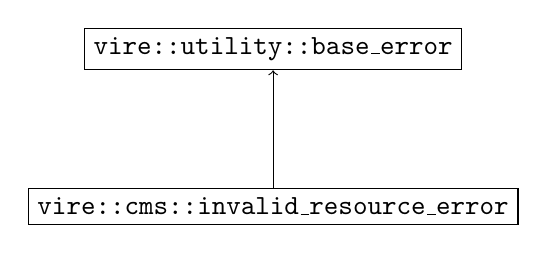
\begin{tikzpicture}
  \node (base)  at (0,2)  [draw] {\texttt{vire::utility::base\_error}};
  \node (ire)  at (0,0) [draw] {\texttt{vire::cms::invalid\_resource\_error}};
  \draw[->] (node cs:name=ire,anchor=north)
  |- (0,1) -| (node cs:name=base,anchor=south);
\end{tikzpicture}
\end{center}

\begin{figure}[h]
\vskip 10pt
\small
\begin{Verbatim}[frame=single,xleftmargin=0.cm,label=\fbox{C++}]
struct vire::cms::invalid_resource_error : public vire::utility::base_error
{
  // Attributes:
  std::string invalid_resource_path; // Invalid resource path
  std::string invalid_resource_id;   // Invalid resource internal ID (Vire server only)
};
\end{Verbatim}
\normalsize
\caption{The structure  of a invalid resource error object (C++).}
\label{fig-app-payload-invalid_resource_error}
\end{figure}

\begin{figure}[h]
\vskip 10pt
\small
\begin{Verbatim}[frame=single,xleftmargin=0.cm,label=\fbox{JSON++}]
{
  "code" : "3",
  "message_format" : "Resource path 'Atlas://Calorimeter/HV/Crate1/stop' is invalid",
  "invalid_resource_path" : "Atlas://Calorimeter/HV/Crate1/stop"
}
\end{Verbatim}
\normalsize
\caption{JSON formatted invalid resource error object.}
\label{fig-app-payload-invalid_resource_error-json}
\end{figure}


\item
Class     \texttt{vire::cms::resource\_status\_record}    (figure
\ref{fig-app-payload-resource_status_record}).

\end{itemize}

\begin{figure}[h]
\vskip 10pt
\small
\begin{Verbatim}[frame=single,xleftmargin=0.cm,label=\fbox{C++}]
struct vire::cms::resource_status_record
{
  // Attributes:
  std::string path;      // Path of the resource
  std::string timestamp; // Timestamp of the last modification
  uint16_t    flags;     // Status bits (Missing/Disabled/Pending/Error)
};
\end{Verbatim}
\normalsize
\caption{The structure  of a resource status record object (C++).}
\label{fig-app-payload-resource_status_record}
\end{figure}


\begin{figure}[h]
\vskip 10pt
\small
\begin{Verbatim}[frame=single,xleftmargin=0.cm,label=\fbox{JSON}]
{
  "path" : "SuperNEMO://Demonstrator/CMS/Coil/Control/Current/__dp_read__",
  "timestamp" : "20160612T212432.324517",
  "flags" : 2
}
\end{Verbatim}
\normalsize
\caption{JSON formatted resource status record object.}
\label{fig-app-payload-resource_status_record-json}
\end{figure}

\vfill
\pagebreak
\clearpage

\subsection{Connection of the Vire server to the CMS server}


\begin{itemize}

\item   The   \texttt{vire::cmslapp::connection\_request}   class
  (version \texttt{1.0})  represents a connection request  sent by the
  Vire server to the  CMS server through the \textcolor{blue}{service}
  channel.

\begin{center}
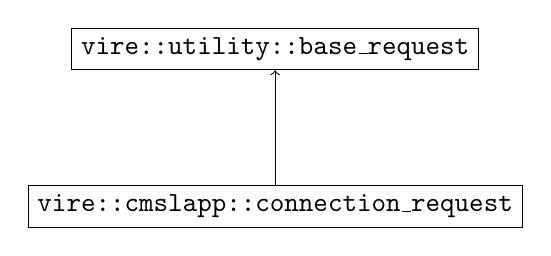
\begin{tikzpicture}
  \node (base)  at (0,2)  [draw] {\texttt{vire::utility::base\_request}};
  \node (cr)  at (0,0) [draw] {\texttt{vire::cmslapp::connection\_request}};
  \draw[->] (node cs:name=cr,anchor=north)
  |- (0,1) -| (node cs:name=base,anchor=south);
\end{tikzpicture}
\end{center}

\noindent Class registration:
\begin{itemize}
\item name: \texttt{"vire::cmslapp::connection\_request"}
\item version: "1.0"
\end{itemize}

\begin{figure}[h]
\vskip 10pt
\small
\begin{Verbatim}[frame=single,xleftmargin=0.cm,label=\fbox{C++}]
struct vire::cmslapp::connection_request : public vire::utility::base_request
{
  // Attributes:
  vire::utility::instance_identifier  setup_id; // Identifier of the experimental setup
  std::vector<std::string> requested_resources; // The list of requested resources
                                                // addressed by path
};
\end{Verbatim}
\normalsize
\caption{The structure of the connection  request object to be emitted
  by the Vire server to the CMS server (C++).}
\label{fig-app-payload-connection_request}
\end{figure}

\begin{figure}[h]
\vskip 10pt
\small
\begin{Verbatim}[frame=single,xleftmargin=0.cm,label=\fbox{JSON}]
{
  "setup_id" : {
    "name" : "snemo",
    "version" : "1.0.2"
  },
  "requested_resources" : [
    "SuperNEMO://Demonstrator/CMS/Coil/PS/Control/Current/__dp_read__",
    "SuperNEMO://Demonstrator/CMS/Coil/PS/Control/Current/__dp_write__",
    ...
    "SuperNEMO://Demonstrator/CMS/Acquisition/start",
    "SuperNEMO://Demonstrator/CMS/Acquisition/stop"
  ]
}
\end{Verbatim}
\normalsize
\caption{A JSON formatted  connection request object sent  by the Vire
  server to the CMS server (C++).}
\label{fig-app-payload-connection_request-json}
\end{figure}


\item  The  \texttt{vire::cmslapp::connection\_success\_response}
  class represents  the response sent back  to the Vire server  by the
  CMS server through the  \textcolor{blue}{service} channel in case of
  success.

\begin{center}
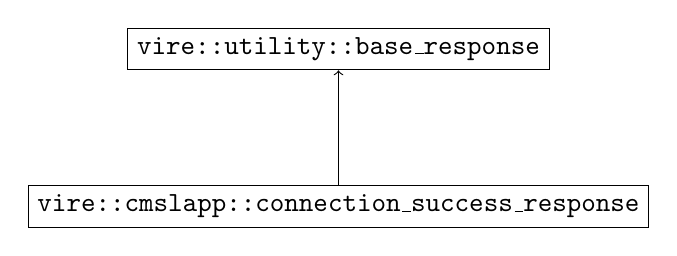
\begin{tikzpicture}
  \node (base)  at (0,2)  [draw] {\texttt{vire::utility::base\_response}};
  \node (csr)  at (0,0) [draw] {\texttt{vire::cmslapp::connection\_success\_response}};
  \draw[->] (node cs:name=csr,anchor=north)
  |- (0,1) -| (node cs:name=base,anchor=south);
\end{tikzpicture}
\end{center}

\noindent Class registration:
\begin{itemize}
\item name: \texttt{"vire::cmslapp::connection\_success\_response"}
\item version: "1.0"
\end{itemize}

\begin{figure}[h]
\vskip 10pt
\small
\begin{Verbatim}[frame=single,xleftmargin=0.cm,label=\fbox{C++}]
struct connection_success_response
  : public vire::utility::base_response
{
  typedef vire::resource::resource_status_record resource_status_record; // Type alias

  // Attributes:
  std::vector<resource_status_record> resources_snapshot; // Requested resources snapshot
};
\end{Verbatim}
\normalsize
\caption{The structure  of the connection success  response emitted by
  the CMS server to the Vire server (C++).}
\label{fig-app-payload-connection_success_response}
\end{figure}



\begin{figure}[h]
\vskip 10pt
\small
\begin{Verbatim}[frame=single,xleftmargin=0.cm,label=\fbox{\texttt{JSON}}]
{
  "resources_snapshot"  : [
    {
      "path" : "SuperNEMO://Demonstrator/CMS/Coil/PS/Control/Current/__dp_read__",
      "timestamp" : "20160612T212432.324517",
      "flags" : "0000"
    },
    {
      "path" : "SuperNEMO://Demonstrator/CMS/Coil/PS/Control/Current/__dp_write__",
      "timestamp" : "20160612T212432.328732",
      "flags" : "0000"
    },
    ...
    {
      "path" : "SuperNEMO://Demonstrator/CMS/Acquisition/start",
      "timestamp" : "20160612T212432.371671",
      "flags" : "0000"
    },
    {
      "path" : "SuperNEMO://Demonstrator/CMS/Acquisition/stop",
      "timestamp" : "20160612T212432.373624",
      "flags" : "0100"
    }
  ]
}
\end{Verbatim}
\normalsize
\caption[JSON formatted  connection success response]  {JSON formatted
  connection        success        response       object        (class
  \texttt{vire::cmslapp::connection\_success\_response}.}
\label{fig-app-payload-connection_success_response-json}
\end{figure}


\item
The  \texttt{vire::cmslapp::connection\_failure\_response}  class
represents the response sent back to the Vire server by the CMS server
through the \textcolor{blue}{service} channel in case of failure.

\begin{center}
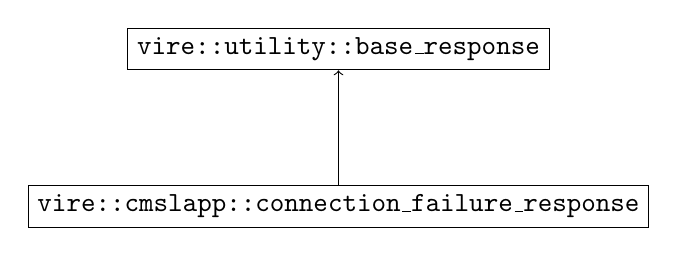
\begin{tikzpicture}
  \node (base)  at (0,2)  [draw] {\texttt{vire::utility::base\_response}};
  \node (cfr)  at (0,0) [draw] {\texttt{vire::cmslapp::connection\_failure\_response}};
  \draw[->] (node cs:name=cfr,anchor=north)
  |- (0,1) -| (node cs:name=base,anchor=south);
\end{tikzpicture}
\end{center}

\begin{figure}[h]
\vskip 10pt
\small
\begin{Verbatim}[frame=single,xleftmargin=0.cm,label=\fbox{C++}]
struct connection_failure_response
  : public vire::utility::base_response
{
  // Nested type alias:
  typedef vire::utility::model_identifier error_identifier;

  // Nested error type aliases:
  typedef vire::utility::invalid_context_error invalid_context_error;
  typedef vire::utility::invalid_setup_id_error invalid_setup_id_error;

  // Nested error type:
  struct unknown_resources_error : public vire::utility::base_error {
    std::vector<std::string> unknown_paths; // List of unknown resources' paths
  };

  // Attributes:
  error_identifier error_id; // Error type identifier
  XXX_error        error;    // Embedded error record of one of the nested error type above
};
\end{Verbatim}
\normalsize
\caption{The structure  of the  connection failure response emitted
  by the CMS server to the Vire server (C++).}
\label{fig-app-payload-connection_failure_response}
\end{figure}


\end{itemize}

% \texttt{vire::cmsserver::disconnection\_request} (version \texttt{1.0})

\vfill
\pagebreak
\clearpage


\subsection{Disconnection of the Vire server from the CMS server}

\begin{itemize}

\item  The  \texttt{vire::cmslapp::disconnection\_request}  class
  represents a  disconnection request sent  by the Vire server  to the
  CMS server through the \textcolor{blue}{service} channel.

\begin{center}
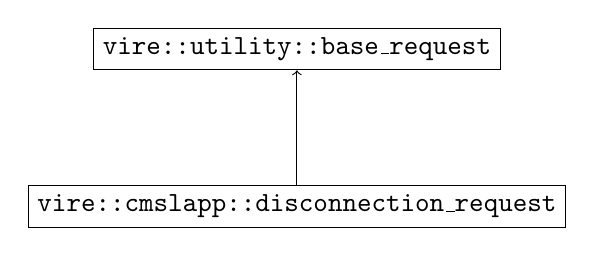
\begin{tikzpicture}
  \node (base)  at (0,2)  [draw] {\texttt{vire::utility::base\_request}};
  \node (cr)  at (0,0) [draw] {\texttt{vire::cmslapp::disconnection\_request}};
  \draw[->] (node cs:name=cr,anchor=north)
  |- (0,1) -| (node cs:name=base,anchor=south);
\end{tikzpicture}
\end{center}

\noindent Class registration:
\begin{itemize}
\item name: \texttt{"vire::cmslapp::disconnection\_request"}
\item version: "1.0"
\end{itemize}

\begin{figure}[h]
\vskip 10pt
\small
\begin{Verbatim}[frame=single,xleftmargin=0.cm,label=\fbox{C++}]
struct disconnection_request : public vire::utility::base_request {
};
\end{Verbatim}
\normalsize
\caption{The structure of the disconnection  request object to be emitted
  by the Vire server to the CMS server (C++).}
\label{fig-app-payload-disconnection_request}
\end{figure}

%% \begin{figure}[h]
%% \vskip 10pt
%% \small
%% \begin{Verbatim}[frame=single,xleftmargin=0.cm,label=\fbox{C++}]
%% {
%% }
%% \end{Verbatim}
%% \normalsize
%% \caption{A JSON formatted  connection request object sent  by the Vire
%%   server to the CMS server (C++).}
%% \label{fig-app-payload-connection_request-json}
%% \end{figure}


\item  The  \texttt{vire::cmslapp::disconnection\_success\_response}
  class represents  the response sent back  to the Vire server  by the
  CMS server through the  \textcolor{blue}{service} channel in case of
  success.

\begin{center}
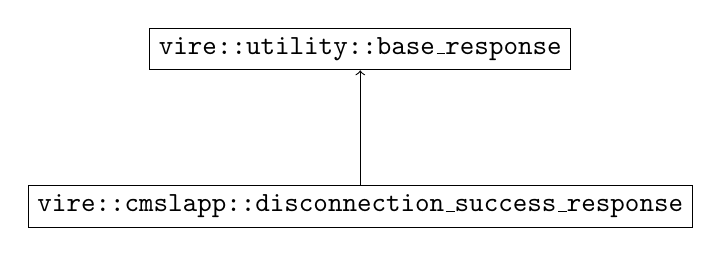
\begin{tikzpicture}
  \node (base)  at (0,2)  [draw] {\texttt{vire::utility::base\_response}};
  \node (csr)  at (0,0) [draw] {\texttt{vire::cmslapp::disconnection\_success\_response}};
  \draw[->] (node cs:name=csr,anchor=north)
  |- (0,1) -| (node cs:name=base,anchor=south);
\end{tikzpicture}
\end{center}


\noindent Class registration:
\begin{itemize}
\item name: \texttt{"vire::cmslapp::disconnection\_success\_response"}
\item version: "1.0"
\end{itemize}

\begin{figure}[h]
\vskip 10pt
\small
\begin{Verbatim}[frame=single,xleftmargin=0.cm,label=\fbox{C++}]
struct disconnection_success_response
  : public vire::utility::base_response
{
};
\end{Verbatim}
\normalsize
\caption{The structure  of the disconnection success  response emitted by
  the CMS server to the Vire server (C++).}
\label{fig-app-payload-disconnection_success_response}
\end{figure}


\end{itemize}


\vfill
\pagebreak
\clearpage

\subsection{Resource related payload objects}

\subsubsection{Resource Pub/Sub service}

\begin{itemize}

\item  The \texttt{vire::resource::resource\_pubsub\_request} object is responsible of
  demanding the activation/deactivation of the Pub/Sub service associated to a given
  resource (fig. \ref{fig-app-payload-resource_pubsub_request}).

\begin{figure}[h]
\vskip 10pt
\small
\begin{Verbatim}[frame=single,xleftmargin=0.cm,label=\fbox{C++}]
struct resource_pubsub_request
  : public vire::utility::base_request
{
  // Attributes:
  std::string path;      // The resource path.
  bool        subscribe; // Pub/Sub service (un)subscribe flag.
};
\end{Verbatim}
\normalsize
\caption{The structure of the \texttt{vire::resource::resource\_pubsub\_request}
  class (C++).}
\label{fig-app-payload-resource_pubsub_request}
\end{figure}

\item The \texttt{vire::resource::resource\_pubsub\_success\_response}
  object encapsulate a  successfull response of the CMS  server to the
  Vire  server  concerning   the  subscription/unsubscription  of  the
  Pub/Sub     service    associated     to     a    given     resource
  (fig. \ref{fig-app-payload-resource_pubsub_success_response}).

\begin{figure}[h]
\vskip 10pt
\small
\begin{Verbatim}[frame=single,xleftmargin=0.cm,label=\fbox{C++}]
struct resource_pubsub_success_response
  : public vire::utility::base_response
{
  // Pub/Sub mechanism type alias:
  typedef vire::resource::amqp_mechanism_address amqp_mechanism_address;

  // Type alias:
  typedef vire::utility::model_identifier pubsub_mechanism_identifier;
  typedef boost::variant<
      amqp_mechanism_address
      > pubsub_address_type;

  // Attributes:
  std::string                 path;               // The resource path.
  bool                        subscribe;          // The effective (un)subscribe flag.
  pubsub_mechanism_identifier pubsub_mechanism_id; // The mechanism for accessing Pub/Sub service
  pubsub_address_type         pubsub_address;      // If activation is set, this describes the
                                                   // access to the Pub/Sub service.
};
\end{Verbatim}
\normalsize
\caption{The structure of the \texttt{vire::resource::resource\_pubsub\_success\_response}
  class (C++).}
\label{fig-app-payload-resource_pubsub_success_response}
\end{figure}

\small
\begin{Verbatim}[frame=single,xleftmargin=0.cm,label=\fbox{JSON++}]
{
  "path" : "SuperNEMO://Demonstrator/CMS/Coil/PS/Monitoring/__dp_read__",
  "subscribe" : "true",
  "pubsub_mechanism_id" : "vire::amqp",
  "pubsub_address" : {
     "server" : "snemo.amqp",
     "port" : 1234,
     "channel" : "snemo.amqp.cms.pubsub.WAqq7ERzs1",
     "binding" : "SuperNEMO://Demonstrator/CMS/Coil/PS/Monitoring/__dp_read__",
     "key" : "coil.monitoring.pubsub"
  }
}
\end{Verbatim}
\normalsize

\item    The   \texttt{vire::resource::amqp\_mechanism\_address}    object
  describes   the  access   to   Pub/Sub   service  through   RabbitMQ
  (fig. \ref{fig-app-payload-amqp_pubsub_access_type}).

\begin{figure}[h]
\vskip 10pt
\small
\begin{Verbatim}[frame=single,xleftmargin=0.cm,label=\fbox{C++}]
struct amqp_mechanism_address
{
  // Attributes:
  std::string server;  // The AMQP server
  int         port;    // The AMQP server port
  std::string channel; // The RabbitMQ Pub/Sub channel.
  std::string binding; // The binding dedicated to this Pub/Sub service.
  std::string key;     // The Pub/Sub specific key/topic.
};
\end{Verbatim}
\normalsize
\caption{The structure of the \texttt{vire::resource::amqp\_pubsub\_access\_type}
  class (C++).}
\label{fig-app-payload-amqp_pubsub_access_type}
\end{figure}


\item The \texttt{vire::resource::resource\_pubsub\_failure\_response}
  object describes a failure response  concerning a request on Pub/Sub
  service       associated       to       a       given       resource
  (fig. \ref{fig-app-payload-resource_pubsub_failure_response}).


\begin{figure}[h]
\vskip 10pt
\small
\begin{Verbatim}[frame=single,xleftmargin=0.cm,label=\fbox{C++}]
struct resource_pubsub_failure_response
  : public vire::utility::base_response
{
  // Nested type alias:
  typedef vire::utility::model_identifier error_type_identifier;

  // Nested error type aliases:
  typedef vire::utility::invalid_context_error  invalid_context_error;
  typedef vire::utility::invalid_resource_error invalid_resource_error;

  // Nested error type:
  struct no_pubsub_resource_error : public vire::utility::base_error {
    std::string path; // The path of the resource without Pub/Sub service support
  };

  typedef boost::variant<
     invalid_context_error,
     invalid_resource_error,
     no_pubsub_resource_error
     > error_type;

  // Attributes:
  error_type_identifier error_type_id; // Error type identifier.
  error_type            error;        // Embedded error record of one of
                                      // the nested error types above.
};
\end{Verbatim}
\normalsize
\caption{The structure of the \texttt{vire::resource::resource\_pubsub\_failure\_response}
  class (C++).}
\label{fig-app-payload-resource_pubsub_failure_response}
\end{figure}

\end{itemize}

\vfill
\pagebreak
\clearpage

\subsubsection{Fetching resource status}

\begin{center}
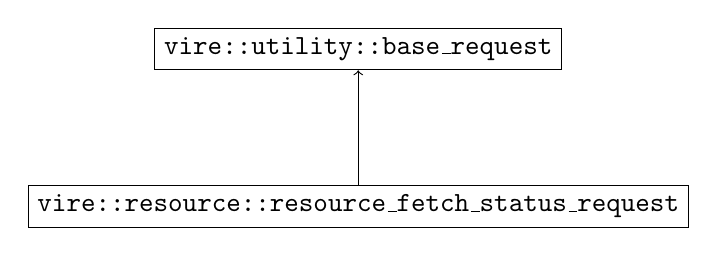
\begin{tikzpicture}
  \node (payload)  at (0,2) [draw] {\texttt{vire::utility::base\_request}};
  \node (request)  at (0,0) [draw] {\texttt{vire::resource::resource\_fetch\_status\_request}};
  \draw[->] (node cs:name=request,anchor=north)
  |- (0,1) -| (node cs:name=payload,anchor=south);
\end{tikzpicture}
\end{center}

\begin{itemize}

\item The \texttt{vire::resource::resource\_fetch\_status\_request} object
  demands to the CMS server an updated status record associated to a given resource
(fig. \ref{fig-app-payload-resource_fetch_status_request}).

\begin{figure}[h]
\vskip 10pt
\small
\begin{Verbatim}[frame=single,xleftmargin=0.cm,label=\fbox{C++}]
struct resource_fetch_status_request
  : public vire::utility::base_request
{
  // Attributes:
  std::string path; // Resource path.
};
\end{Verbatim}
\normalsize
\caption{The structure of a \texttt{vire::utility::resource\_fetch\_status\_request} object
  (C++).}
\label{fig-app-payload-resource_fetch_status_request}
\end{figure}

\item The \texttt{vire::resource::resource\_fetch\_status\_success\_response} object
  transmits the updated/current status record  associated to a given resource
(fig. \ref{fig-app-payload-resource_fetch_status_success_response}).

\begin{figure}[h]
\vskip 10pt
\small
\begin{Verbatim}[frame=single,xleftmargin=0.cm,label=\fbox{C++}]
struct resource_fetch_status_success_response
  : public vire::utility::base_response
{
  // Nested type alias:
  typedef vire::resource::resource_status_record resource_status_record;

  // Attributes:
  resource_status_record status; // The resource status record.
};
\end{Verbatim}
\normalsize
\caption{The structure of a \texttt{vire::utility::resource\_fetch\_status\_success\_response} object
  (C++).}
\label{fig-app-payload-resource_fetch_status_success_response}
\end{figure}



\item The \texttt{vire::resource::resource\_fetch\_status\_failure\_response} object
  describes a failure detected by the CMS server in response to a resource fetch status request.

\begin{figure}[h]
\vskip 10pt
\small
\begin{Verbatim}[frame=single,xleftmargin=0.cm,label=\fbox{C++}]
struct resource_fetch_status_failure_response
  : public vire::utility::base_response
{
  // Nested type alias:
  typedef vire::utility::model_identifier error_identifier;

  // Nested error type aliases:
  typedef vire::utility::invalid_context_error   invalid_context_error;
  typedef vire::resource::invalid_resource_error invalid_resource_error;

  // Attributes:
  error_identifier error_id; // Error type identifier
  XXX_error        error;    // Embedded error record of one of the nested error type above
};
\end{Verbatim}
\normalsize
\caption{The structure of a \texttt{vire::utility::resource\_fetch\_status\_failure\_response} object
  (C++).}
\label{fig-app-payload-resource_fetch_status_failure_response}
\end{figure}


\end{itemize}


\vfill
\pagebreak
\clearpage

\subsubsection{Synchronous/blocking resource execution}

\begin{center}
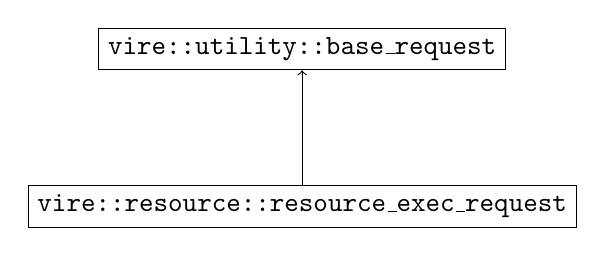
\begin{tikzpicture}
  \node (payload)  at (0,2)   [draw] {\texttt{vire::utility::base\_request}};
  \node (request)  at (0,0)  [draw] {\texttt{vire::resource::resource\_exec\_request}};
  \draw[->] (node cs:name=request,anchor=north)
  |- (0,1) -| (node cs:name=payload,anchor=south);
\end{tikzpicture}
\end{center}

\begin{itemize}

\item The \texttt{vire::resource::resource\_exec\_request} object represent a resource execution request
in blocking (synchronous) mode.


\begin{figure}[h]
\vskip 10pt
\small
\begin{Verbatim}[frame=single,xleftmargin=0.cm,label=\fbox{C++}]
struct resource_exec_request
  : public vire::utility::base_request
{
  // Type alias:
  typedef vire::resource::method_argument method_argument;

  // Attributes:
  std::string                  path;            // Resource path.
  std::vector<method_argument> input_arguments; // Embedded error record of one of
                                                // the nested error type above.
};
\end{Verbatim}
\normalsize
\caption{The structure of a \texttt{vire::utility::resource\_fetch\_status\_failure\_response} object
  (C++).}
\label{fig-app-payload-resource_fetch_status_failure_response}
\end{figure}

\item \texttt{vire::resource::resource\_exec\_success\_response}

\small
\begin{Verbatim}[frame=single,xleftmargin=0.cm,label=\fbox{C++}]
struct resource_exec_success_response
 : vire::utility::base_response
{
  // Type alias:
  typedef vire::resource::method_argument        method_argument;
  typedef vire::resource::resource_status_record resource_status_record;

  // Attributes:
  resource_status_record       status;               // Resource status
  std::string                  reception_timestamp;  // Request reception timestamp
  std::string                  completion_timestamp; // Execution completion timestamp
  std::vector<method_argument> output_arguments;     // Output arguments
};
\end{Verbatim}



\item \texttt{vire::resource::resource\_exec\_failure\_response}


\small
\begin{Verbatim}[frame=single,xleftmargin=0.cm,label=\fbox{C++}]
struct resource_exec_failure_response
 : vire::utility::base_response
{

  // Error type aliases:
  typedef vire::utility::invalid_context_error   invalid_context_error;
  typedef vire::resource::invalid_resource_error invalid_resource_error;
  typedef vire::resource::invalid_status_error   invalid_status_error;
  typedef vire::resource::resource_exec_error    resource_exec_error;

  // Type aliases:
  typedef vire::utility::model_identifier        error_type_identifier;
  typedef boost::variant<
      invalid_context_error,
      invalid_resource_error,
      invalid_status_error,
      resource_exec_error> error_type;

  // Attributes:
  error_type_identifier error_type_id; // Error type identifier
  error_type            error;        // Embedded error record

};
\end{Verbatim}

\end{itemize}


\vfill
\pagebreak
\clearpage

\subsubsection{Asynchronous/non-blocking resource execution}

\begin{center}
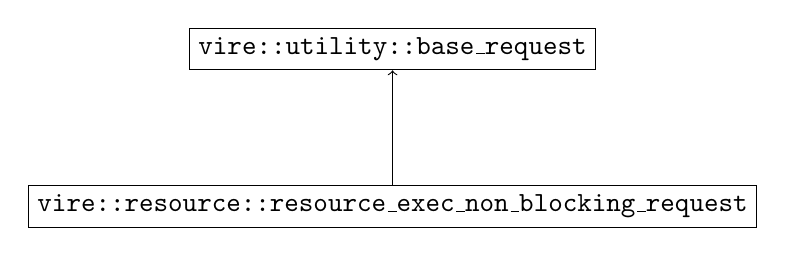
\begin{tikzpicture}
  \node (payload)  at (0,2)   [draw] {\texttt{vire::utility::base\_request}};
  \node (request_nb)  at (0,0)  [draw] {\texttt{vire::resource::resource\_exec\_non\_blocking\_request}};
  \draw[->] (node cs:name=request_nb,anchor=north)
  |- (0,1) -| (node cs:name=payload,anchor=south);
\end{tikzpicture}
\end{center}

\begin{itemize}

\item \texttt{vire::resource::resource\_exec\_non\_blocking\_request}
\small
\begin{Verbatim}[frame=single,xleftmargin=0.cm,label=\fbox{C++}]
struct resource_exec_non_blocking_request
  : public vire::utility::base_request
{
  // Type alias:
  typedef vire::resource::method_argument method_argument;

  // Attributes:
  std::string                  path;            // Resource path.
  std::vector<method_argument> input_arguments; // Embedded error record of one of
                                                // the nested error type above.

};
\end{Verbatim}

\item \texttt{vire::resource::resource\_exec\_non\_blocking\_ack\_response}


\small
\begin{Verbatim}[frame=single,xleftmargin=0.cm,label=\fbox{C++}]
struct resource_exec_non_blocking_ack_response
 : vire::utility::base_response
{
  // Type alias:
  typedef vire::resource::method_argument        method_argument;
  typedef vire::resource::resource_status_record resource_status_record;

  // Attributes:
  resource_status_record       status;
  std::string                  reception_timestamp;

};
\end{Verbatim}


\item \texttt{vire::resource::resource\_exec\_non\_blocking\_noack\_response}


\small
\begin{Verbatim}[frame=single,xleftmargin=0.cm,label=\fbox{C++}]
struct resource_exec_non_blocking_noack_response
  : vire::utility::base_response
{
  // Type alias:
  typedef vire::resource::resource_status_record resource_status_record;
  typedef vire::utility::model_identifier error_type_identifier;

  // Error type aliases:
  typedef vire::utility::invalid_context_error   invalid_context_error;
  typedef vire::resource::invalid_resource_error invalid_resource_error;
  typedef vire::resource::invalid_status_error   invalid_status_error;
  typedef vire::resource::resource_exec_error    resource_exec_error;

  // Nested error type:
  struct no_non_blocking_exec_resource_error : public vire::utility::base_error {
    std::string path; // The path of the resource without non-blocking execution support
  };

  typedef boost::variant<
     invalid_context_error,
     invalid_resource_error,
     invalid_status_error,
     no_non_blocking_exec_resource_error,
     resource_exec_error
     > error_type;

  // Attributes:
  resource_status_record status;        // Resource status.
  error_type_identifier  error_type_id; // Error type identifier.
  error_type             error;         // Embedded error record of one of
                                        // the nested error types above.

};
\end{Verbatim}
\normalsize


\item \texttt{vire::resource::resource\_exec\_non\_blocking\_success\_event}


\small
\begin{Verbatim}[frame=single,xleftmargin=0.cm,label=\fbox{C++}]
struct resource_exec_non_blocking_success\_event
  : vire::utility::base_event
{
  // Type alias:
  typedef vire::resource::method_argument        method_argument;
  typedef vire::resource::resource_status_record resource_status_record;

  // Attributes:
  resource_status_record       status;               // Resource status
  std::string                  reception_timestamp;  // Request reception timestamp
  std::string                  completion_timestamp; // Execution completion timestamp
  std::vector<method_argument> output_arguments;     // Output arguments

};
\end{Verbatim}
\normalsize

\item \texttt{vire::resource::resource\_exec\_non\_blocking\_failure\_event}


\small
\begin{Verbatim}[frame=single,xleftmargin=0.cm,label=\fbox{C++}]
struct resource_exec_non_blocking_failure\_event
  : vire::utility::base_event
{

  // Error type aliases:
  typedef vire::utility::invalid_context_error   invalid_context_error;
  typedef vire::cms::invalid_resource_error invalid_resource_error;
  typedef vire::cms::invalid_status_error   invalid_status_error;
  typedef vire::cms::resource_exec_error    resource_exec_error;

  // Type aliases:
  typedef vire::utility::model_identifier        error_type_identifier;
  typedef boost::variant<
      vire::utility::invalid_context_error,
      vire::cms::invalid_resource_error,
      vire::cms::invalid_status_error,
      vire::cms::resource_exec_error> error_type;

  // Attributes:
  error_type_identifier error_type_id; // Error type identifier
  error_type            error;        // Embedded error record

};
\end{Verbatim}
\normalsize


\end{itemize}


\vfill
\pagebreak
\clearpage

% end


\section{The RabbitMQ based RPC system}\label{app:rabbitmq_rpc}

\subsection{Introduction}


\end{document}
%%

\vfill
\pagebreak
\clearpage

\documentclass[a4paper,11pt,twoside]{article}

%%% packages:
\usepackage[T1]{fontenc}
\usepackage{ucs}
\usepackage[utf8x]{inputenc}
%\usepackage[frenchb]{babel}
\usepackage{amsmath}
\usepackage{amssymb}
\usepackage{latexsym}
\usepackage{verbatim}
\usepackage{moreverb}
\usepackage{fancyvrb}
\usepackage{alltt}
\usepackage{eurosym}
\usepackage{hyperref}
\usepackage{colortbl}
\usepackage{graphicx}
\usepackage{pdflscape}
\usepackage{afterpage}
\usepackage{rotating}
\usepackage{tikz}
%\usepackage{tikz-qtree}

%%% Geometry (https://en.wikibooks.org/wiki/LaTeX/Page_Layout)
\usepackage{layout}
%\usepackage[a4paper,top=1in, bottom=1.25in, left=1.25in, right=1.25in, inner=4cm,outer=2cm]{geometry}
\usepackage[a4paper,inner=2cm,outer=2cm]{geometry}
%% \setlength{\hoffset}{-1inch}
%% \setlength{\voffset}{-1inch0pt}
\setlength{\textheight}{23cm}
%% \setlength{\textwidth}{18cm}

%%% macros:
\newcommand{\thepath}{.}
\newcommand{\imgpath}{\thepath/images}
\newcommand{\pdfteximgpath}{\thepath/pdftex}
\newcommand{\pdftextimgpath}{\thepath/pdftex_t}

%%%
\title{The SuperNEMO Vire-CMS/LAPP interface\\version 0.7}
\author{E.Chabanne, J.Hommet, T. Leflour, Y. Lemière,
  S.Lieunard, F.Mauger, J.-L. Panazol, J.Poincheval}
\date{\today}

%%%
\begin{document}

\thispagestyle{empty}
%\layout{}
\maketitle
\begin{abstract}
This document aims  to describe the requirements of  the Vire CMS/LAPP
interface,  i.e. the  software bridge  between the  Vire based  online
software  (Vire server  and clients,  a.k.a the  Vire system)  and the
CMS/LAPP server  that plays  the role  of the  unique gate  (subcontractor proxy) to
communicate with  the OPCUA-based MOS  servers responsible of  the low
level control and monitoring operations on some hardware devices.
\end{abstract}
\vfill
\pagebreak

\tableofcontents
\vfill
\pagebreak

\listoffigures
\vfill
\pagebreak

\listoftables
\vfill
\pagebreak
\clearpage

\documentclass[a4paper,11pt,twoside]{article}

%%% packages:
\usepackage[T1]{fontenc}
\usepackage{ucs}
\usepackage[utf8x]{inputenc}
%\usepackage[frenchb]{babel}
\usepackage{amsmath}
\usepackage{amssymb}
\usepackage{latexsym}
\usepackage{verbatim}
\usepackage{moreverb}
\usepackage{fancyvrb}
\usepackage{alltt}
\usepackage{eurosym}
\usepackage{hyperref}
\usepackage{colortbl}
\usepackage{graphicx}
\usepackage{pdflscape}
\usepackage{afterpage}
\usepackage{rotating}
\usepackage{tikz}
%\usepackage{tikz-qtree}

%%% Geometry (https://en.wikibooks.org/wiki/LaTeX/Page_Layout)
\usepackage{layout}
%\usepackage[a4paper,top=1in, bottom=1.25in, left=1.25in, right=1.25in, inner=4cm,outer=2cm]{geometry}
\usepackage[a4paper,inner=2cm,outer=2cm]{geometry}
%% \setlength{\hoffset}{-1inch}
%% \setlength{\voffset}{-1inch0pt}
\setlength{\textheight}{23cm}
%% \setlength{\textwidth}{18cm}

%%% macros:
\newcommand{\thepath}{.}
\newcommand{\imgpath}{\thepath/images}
\newcommand{\pdfteximgpath}{\thepath/pdftex}
\newcommand{\pdftextimgpath}{\thepath/pdftex_t}

%%%
\title{The SuperNEMO Vire-CMS/LAPP interface\\version 0.7}
\author{E.Chabanne, J.Hommet, T. Leflour, Y. Lemière,
  S.Lieunard, F.Mauger, J.-L. Panazol, J.Poincheval}
\date{\today}

%%%
\begin{document}

\thispagestyle{empty}
%\layout{}
\maketitle
\begin{abstract}
This document aims  to describe the requirements of  the Vire CMS/LAPP
interface,  i.e. the  software bridge  between the  Vire based  online
software  (Vire server  and clients,  a.k.a the  Vire system)  and the
CMS/LAPP server  that plays  the role  of the  unique gate  (subcontractor proxy) to
communicate with  the OPCUA-based MOS  servers responsible of  the low
level control and monitoring operations on some hardware devices.
\end{abstract}
\vfill
\pagebreak

\tableofcontents
\vfill
\pagebreak

\listoffigures
\vfill
\pagebreak

\listoftables
\vfill
\pagebreak
\clearpage

\input{cms_server/main.tex}
\vfill
\pagebreak
\clearpage

\input{vire_resources/main.tex}
\vfill
\pagebreak
\clearpage

% \input{cmslapp_vireclients/main.tex}
\section{Interaction of the CMS/LAPP server with Vire clients}

TODO
\vfill
\pagebreak
\clearpage

%%%%%%%%%
\appendix

\input{appendix/app_filesystem.tex}
\input{appendix/app_new_device.tex}
\input{appendix/app_vire_messages.tex}
%\input{appendix/app_json_fmt.tex}
\input{appendix/app_protobuf_format.tex}
\input{appendix/app_payload_objects.tex}
\input{appendix/app_rabbitmq_rpc.tex}

\end{document}
%%

\vfill
\pagebreak
\clearpage

\documentclass[a4paper,11pt,twoside]{article}

%%% packages:
\usepackage[T1]{fontenc}
\usepackage{ucs}
\usepackage[utf8x]{inputenc}
%\usepackage[frenchb]{babel}
\usepackage{amsmath}
\usepackage{amssymb}
\usepackage{latexsym}
\usepackage{verbatim}
\usepackage{moreverb}
\usepackage{fancyvrb}
\usepackage{alltt}
\usepackage{eurosym}
\usepackage{hyperref}
\usepackage{colortbl}
\usepackage{graphicx}
\usepackage{pdflscape}
\usepackage{afterpage}
\usepackage{rotating}
\usepackage{tikz}
%\usepackage{tikz-qtree}

%%% Geometry (https://en.wikibooks.org/wiki/LaTeX/Page_Layout)
\usepackage{layout}
%\usepackage[a4paper,top=1in, bottom=1.25in, left=1.25in, right=1.25in, inner=4cm,outer=2cm]{geometry}
\usepackage[a4paper,inner=2cm,outer=2cm]{geometry}
%% \setlength{\hoffset}{-1inch}
%% \setlength{\voffset}{-1inch0pt}
\setlength{\textheight}{23cm}
%% \setlength{\textwidth}{18cm}

%%% macros:
\newcommand{\thepath}{.}
\newcommand{\imgpath}{\thepath/images}
\newcommand{\pdfteximgpath}{\thepath/pdftex}
\newcommand{\pdftextimgpath}{\thepath/pdftex_t}

%%%
\title{The SuperNEMO Vire-CMS/LAPP interface\\version 0.7}
\author{E.Chabanne, J.Hommet, T. Leflour, Y. Lemière,
  S.Lieunard, F.Mauger, J.-L. Panazol, J.Poincheval}
\date{\today}

%%%
\begin{document}

\thispagestyle{empty}
%\layout{}
\maketitle
\begin{abstract}
This document aims  to describe the requirements of  the Vire CMS/LAPP
interface,  i.e. the  software bridge  between the  Vire based  online
software  (Vire server  and clients,  a.k.a the  Vire system)  and the
CMS/LAPP server  that plays  the role  of the  unique gate  (subcontractor proxy) to
communicate with  the OPCUA-based MOS  servers responsible of  the low
level control and monitoring operations on some hardware devices.
\end{abstract}
\vfill
\pagebreak

\tableofcontents
\vfill
\pagebreak

\listoffigures
\vfill
\pagebreak

\listoftables
\vfill
\pagebreak
\clearpage

\input{cms_server/main.tex}
\vfill
\pagebreak
\clearpage

\input{vire_resources/main.tex}
\vfill
\pagebreak
\clearpage

% \input{cmslapp_vireclients/main.tex}
\section{Interaction of the CMS/LAPP server with Vire clients}

TODO
\vfill
\pagebreak
\clearpage

%%%%%%%%%
\appendix

\input{appendix/app_filesystem.tex}
\input{appendix/app_new_device.tex}
\input{appendix/app_vire_messages.tex}
%\input{appendix/app_json_fmt.tex}
\input{appendix/app_protobuf_format.tex}
\input{appendix/app_payload_objects.tex}
\input{appendix/app_rabbitmq_rpc.tex}

\end{document}
%%

\vfill
\pagebreak
\clearpage

% \documentclass[a4paper,11pt,twoside]{article}

%%% packages:
\usepackage[T1]{fontenc}
\usepackage{ucs}
\usepackage[utf8x]{inputenc}
%\usepackage[frenchb]{babel}
\usepackage{amsmath}
\usepackage{amssymb}
\usepackage{latexsym}
\usepackage{verbatim}
\usepackage{moreverb}
\usepackage{fancyvrb}
\usepackage{alltt}
\usepackage{eurosym}
\usepackage{hyperref}
\usepackage{colortbl}
\usepackage{graphicx}
\usepackage{pdflscape}
\usepackage{afterpage}
\usepackage{rotating}
\usepackage{tikz}
%\usepackage{tikz-qtree}

%%% Geometry (https://en.wikibooks.org/wiki/LaTeX/Page_Layout)
\usepackage{layout}
%\usepackage[a4paper,top=1in, bottom=1.25in, left=1.25in, right=1.25in, inner=4cm,outer=2cm]{geometry}
\usepackage[a4paper,inner=2cm,outer=2cm]{geometry}
%% \setlength{\hoffset}{-1inch}
%% \setlength{\voffset}{-1inch0pt}
\setlength{\textheight}{23cm}
%% \setlength{\textwidth}{18cm}

%%% macros:
\newcommand{\thepath}{.}
\newcommand{\imgpath}{\thepath/images}
\newcommand{\pdfteximgpath}{\thepath/pdftex}
\newcommand{\pdftextimgpath}{\thepath/pdftex_t}

%%%
\title{The SuperNEMO Vire-CMS/LAPP interface\\version 0.7}
\author{E.Chabanne, J.Hommet, T. Leflour, Y. Lemière,
  S.Lieunard, F.Mauger, J.-L. Panazol, J.Poincheval}
\date{\today}

%%%
\begin{document}

\thispagestyle{empty}
%\layout{}
\maketitle
\begin{abstract}
This document aims  to describe the requirements of  the Vire CMS/LAPP
interface,  i.e. the  software bridge  between the  Vire based  online
software  (Vire server  and clients,  a.k.a the  Vire system)  and the
CMS/LAPP server  that plays  the role  of the  unique gate  (subcontractor proxy) to
communicate with  the OPCUA-based MOS  servers responsible of  the low
level control and monitoring operations on some hardware devices.
\end{abstract}
\vfill
\pagebreak

\tableofcontents
\vfill
\pagebreak

\listoffigures
\vfill
\pagebreak

\listoftables
\vfill
\pagebreak
\clearpage

\input{cms_server/main.tex}
\vfill
\pagebreak
\clearpage

\input{vire_resources/main.tex}
\vfill
\pagebreak
\clearpage

% \input{cmslapp_vireclients/main.tex}
\section{Interaction of the CMS/LAPP server with Vire clients}

TODO
\vfill
\pagebreak
\clearpage

%%%%%%%%%
\appendix

\input{appendix/app_filesystem.tex}
\input{appendix/app_new_device.tex}
\input{appendix/app_vire_messages.tex}
%\input{appendix/app_json_fmt.tex}
\input{appendix/app_protobuf_format.tex}
\input{appendix/app_payload_objects.tex}
\input{appendix/app_rabbitmq_rpc.tex}

\end{document}
%%

\section{Interaction of the CMS/LAPP server with Vire clients}

TODO
\vfill
\pagebreak
\clearpage

%%%%%%%%%
\appendix


\section{Filesystem and configuration files management}\label{app:filesystem_conf}

Let's consider  a simple  situation where  one runs  the Vire  and CMS
software  tools (servers)  on a  single Linux  machine (the  CMS host)
under            the            \texttt{"nemoprod"}            generic
account\footnote{\texttt{"nemoprod"}  is  the   login  of  th  generic
  account used at the CCIN2P3  cluster to perform automated management
  operations on experimental and  Monte-Carlo data file: data transfer
  from LSM or LSC labs to CCIN2P3, calibration and reconstruction data
  processing, storage on HPPS.}.

\begin{itemize}
\item Hostname login : \verb|192.168.1.10| (private IP) %\texttt{snemocms.lsm.in2p3.fr} (public address)
\item User login : \texttt{nemoprod}
\item Main group : \texttt{supernemo}
\item Home directory : \verb|/home/nemoprod| (a.k.a. \verb|~nemoprod|)
\end{itemize}

\noindent  We  assume that  the  SuperNEMO  online software  has  been
installed   and  setup   in  the   home  directory,   for  example in
\verb|/home/nemoprod/Private/Software/| :
\vskip 20pt
\small
\begin{Verbatim}[frame=single,xleftmargin=0.cm,label=\fbox{Filesystem}]
/home/nemoprod/Private/Software
|-- Cadfael/ # base directory of the Cadfael software framework
|-- Bayeux/  # base directory of the Bayeux software framework
|-- Vire/    # base directory of the Vire software framework
|-- OPCUA/   # base directory of the OPCUA+MOS software framework
`-- Falaise/ # base directory of the Falaise software framework
\end{Verbatim}
\normalsize

\noindent  We consider  here  that the  Falaise  library package  will
contain  the mandatory  configuration files  that describe  the online
software, both for the Vire and CMS/MOS parts:
\vskip 20pt
\small
\begin{Verbatim}[frame=single,xleftmargin=0.cm,label=\fbox{Filesystem}]
/home/nemoprod/Private/Software
:
`-- Falaise/
    :
    `-- Install/
        `-- Falaise-3.0.0/
            |-- bin/
            |   :
            |   |-- flquery
            |   |-- flreconstruct
            |   `-- flsimulate
            |-- include/
            :   :
            |-- lib/
            |   `-- x86_64-linux-gnu/
            |       :
            |       |-- libFalaise.so
            |       :
            `-- share/
                `-- Falaise-3.0.0/
                    `-- resources/
                        `-- config/
                            `-- online/
                                :
                                :
\end{Verbatim}
\normalsize

\noindent Where:
\begin{itemize}
\item                                                              the
  \verb|/home/nemoprod/Private/Software/Falaise/Install/Falaise-3.0.0|
  is  the  installation  prefix  of  the  Falaise  library  (binaries,
  includes) and associated resource files.
\item      the     \verb|share/Falaise-3.0.0/resources/config/online/|
  subdirectory  is the  tree  of configuration  files  that should  be
  accessible  by  any online  software  component  (Vire server,  Vire
  clients, CMS and MOS servers).
\end{itemize}


\noindent  Let's consider  the \verb|.../config/online/|  directory as
the base directory for all online configuration files for the Vire and
CMS  servers.   All  configuration  files  should  thus  be  addressed
relatively to this place.

\noindent  We  propose to  use  one  of  the following  techniques  to
represent this base directory:

\begin{itemize}
\item         a         dedicated         environment         variable
  \verb|SNEMO_ONLINE_CONFIG_BASE_DIR| recognized by  both Vire and CMS
  servers. It could be setup within the environment with:
\vskip 20pt
\small
\begin{Verbatim}[frame=single,xleftmargin=0.cm,label=\fbox{shell}]
export FALAISE_INSTALL_DIR=\
  ${HOME}/Private/Software/Falaise/Install/Falaise-3.0.0
export SNEMO_ONLINE_CONFIG_BASE_DIR=\
  ${FALAISE_INSTALL_DIR}/share/Falaise-3.0.0/resources/config/online
\end{Verbatim}
\normalsize

\item a  path registration label as  implemented in the kernel  of the
  Bayeux library:\\
  \noindent The \verb|@snonlinecfg:| label \\
  is associated to\\
  \noindent \hskip 50pt\verb|${FALAISE_INSTALL_DIR}/share/Falaise-3.0.0/resources/config/online|

\end{itemize}

\noindent Thus a specific  configuration file \verb|dummy.conf| could be
addressed with one of the following syntaxes:

\begin{itemize}

\item[(a)]
  \verb|${SNEMO_ONLINE_CONFIG_BASE_DIR}/snemo/1.0.2/dummy.conf|       :
  supported  by  Vire  and  CMS  using  word  expansion  utility  like
  \texttt{wordexp} (for C/C++ languages),

\item[(b)]  \verb|@snonlinecfg:snemo/1.0.2/dummy.conf|  : supported  by
  Vire  only  for  now,  thanks to  the  path  registration  mechanism
  implemented in the Bayeux API,

\item[(c)] \verb|snemo/1.0.2/dummy.conf| : can be supported by Vire and
  CMS  but  is  ambiguous  because  such a relative  path  can  be  also
  interpreted as a path relatively  to the current directory (\verb|./|)
  and not to the online configuration directory.

\end{itemize}

We suggests  the use  of an  explicit environment  variable as  in (a)
because it  is simple to  implement in various languages  and software
frameworks and should not imply any ambiguous file path resolution.

\vfill
\pagebreak
\clearpage

% end


\section{Integration of a new device}\label{app:new_device}

Both Vire  and MOS systems are  designed to be expandable  in terms of
device integration.  This section  decribes the  integration of  a new
device in the \emph{Control and Monitoring System}.

\subsection{Integration of a new device in the MOS environment}

Any new device is described through  a dedicated XML model file.  This
XML  file  is  created  from  a  template  file  elaborated  from  the
\emph{interface control document} (ICD) and associated to the model of
the  device. The  format  of the  XML  file is  described  in the  MOS
(Multipurpose OPCUA Server) User Guide. % ref

Typically, a device is embedded in a OPCUA server and implemented as a
OPCUA  \emph{simple  device}.   The  OPCUA server  itself  is  located
through an unique dedicated IP address and port.

The simple device  instance, hosted in the OPCUA  server, may contains
other sub-devices and/or \emph{datapoints}.   It is thus considered as
the root  of a hierarchy  of daughter  objects at deeper  levels.  The
daughter objects (devices or datapoints) are named relatively to their
top level  parent device. Figure  \ref{fig:an:mos_dev_1} shows an
example of a device embedded in a MOS server.

\begin{figure}[h]
\begin{center}
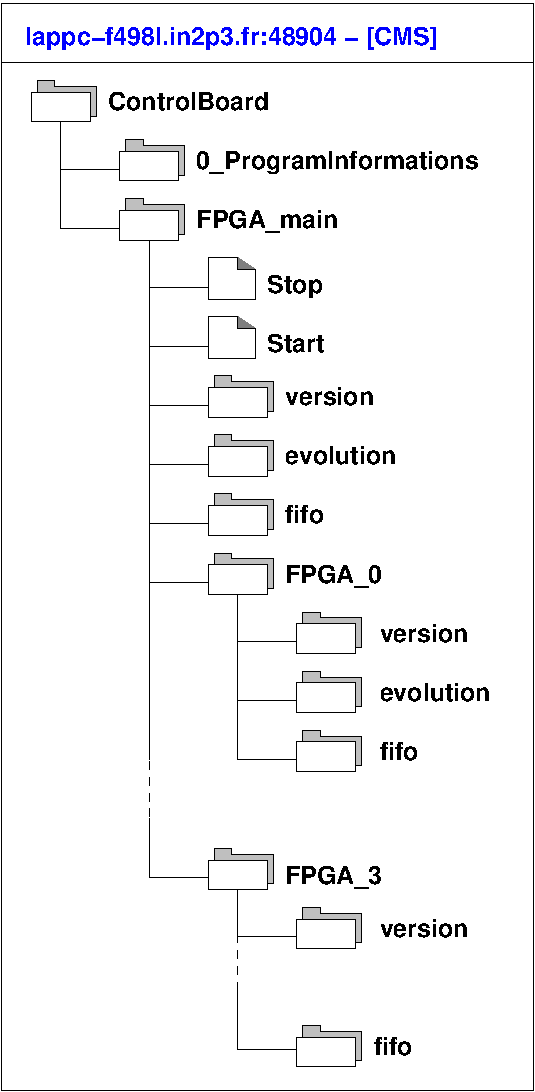
\includegraphics[width=5cm]{appendix/images/MOS_device_example_1.pdf}
\end{center}
\caption{Example of a  device managed through a MOS  server.  The root
  device is named \texttt{ControlBoard}.  First level daughter devices
  are  \texttt{0\_ProgramInformations} and  \texttt{FPGA\_main}.  Here
  the          MOS/OPCUA          server          is          labelled
  \texttt{CMS}.}\label{fig:an:mos_dev_1}
\end{figure}

% TODO


\subsection{Integration of a new device in the Vire environment}

The Vire  API also implements a  mechanism to describe a  hierarchy of
devices.  This  mechanism is independant  of the  one used in  the MOS
system but can  be easily made compatible with it.   This means that a
MOS  hierarchy  of devices  can  be  represented  in Vire.   The  Vire
hierarchy of  devices can  be considered as  some kind  of filesystem,
each device  being a folder with  its unique path, as  shown on figure
\ref{fig:an:mos_dev_2}.   The \emph{methods}  associated to  a devices
(or a datapoint) can be considered as plain executable files stored in
the  device's folder  : they  constitute the  set of  \emph{resources}
associated to the device.


\begin{figure}[h]
\begin{center}
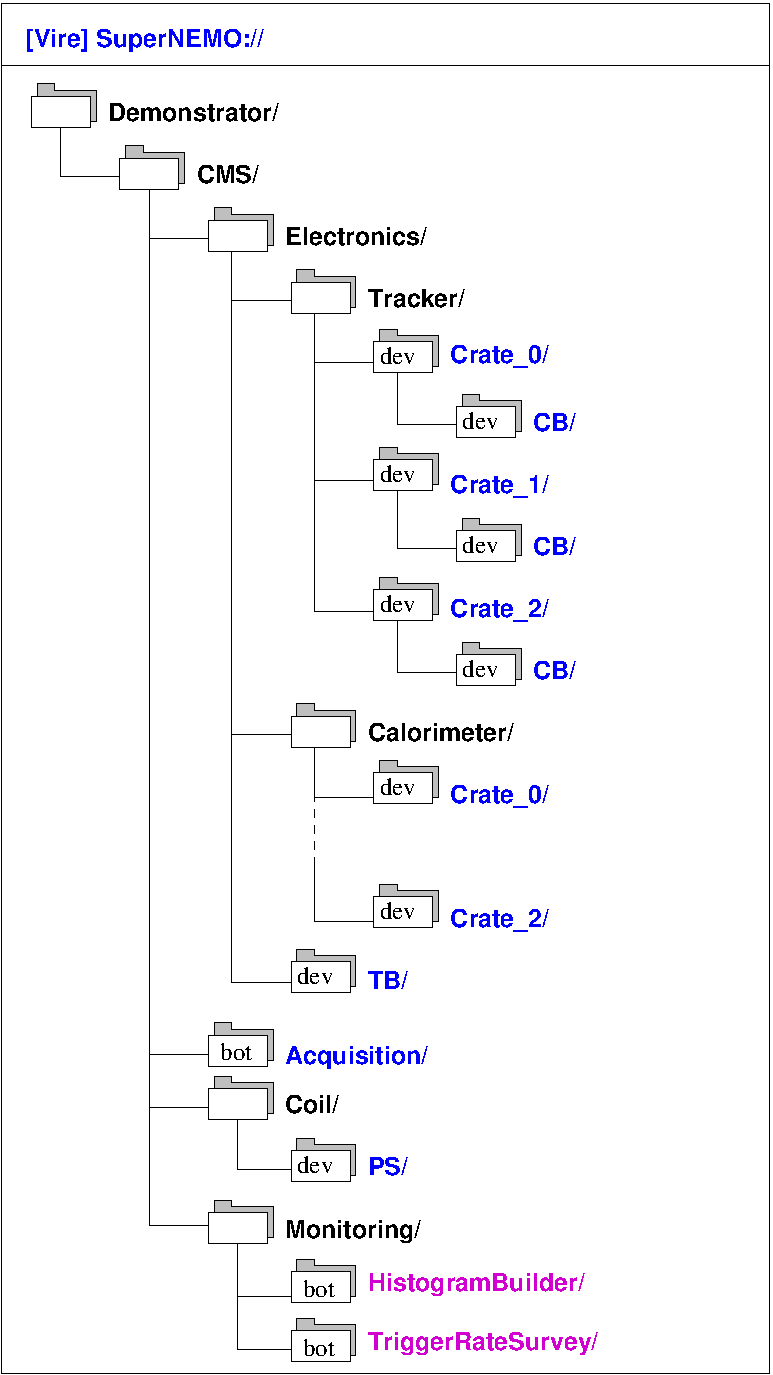
\includegraphics[width=5cm]{appendix/images/MOS_device_example_2.pdf}
\end{center}
\caption{Example of a hierarchy of  devices described by the Vire API.
  The root device is named  \texttt{SuperNEMO:}.  The top level (root)
  device  is  named  \texttt{Demonstrator}.  The  devices  colored  in
  \textcolor{blue}{blue}  are managed  through MOS/OPCUA.  The devices
  colored in \textcolor{magenta}{magenta} are directly embedded in the
  Vire server.  Devices with the \texttt{dev} tag are typical hardware
  device.  Devices  with the  \texttt{bot}  tag  are typical  software
  devices.   The  devices  colored in  \textbf{black}  are  structural
  pseudo-devices used to organize and  present a comprehensive view of
  the hierarchy. }\label{fig:an:mos_dev_2}
\end{figure}

The organisation of this hierarchy of devices is arbitrary and defined
by the designer of the  \emph{Control and Monitoring System}.  What is
important  to  understand  is  that  some  of  these  devices  can  be
associated  to  \emph{hardware  devices}  (a  power  supply  crate,  a
temperature probe\dots) and others  can be \emph{pseudo-devices}, i.e.
pure   software  object   (a   monitoring  robot,   a  file   transfer
daemon\dots).

In the context of the coupling of  the Vire server and the CMS server,
we are  in the event that  some devices are managed  by some MOS/OPCUA
servers and others are managed  in the Vire server itself.  Typically,
\emph{hardware devices}  are systematically managed through  the OPCUA
technology.  Vire has a mechanism to integrate such devices in its own
hierarchy.  This mechanism can  be considered like the \emph{mounting}
of   a   remote   filesystem   from  a   local   filesystem.    Figure
\ref{fig:an:mos_dev_0} illustrates  the case of many  hardware devices
-- managed by MOS -- that are integrated in the Vire system.  From the
Vire point of  view, the user does not see  the implementation details
for such  devices. He  does not  know the identity  of the  MOS server
hosting the device. He does not even know if the device is hosted by a
MOS server.  Devices are simply visible through the standard hierarchy
published by Vire with its  own device naming scheme, regardless their
true location.



\begin{figure}[h]
\begin{center}
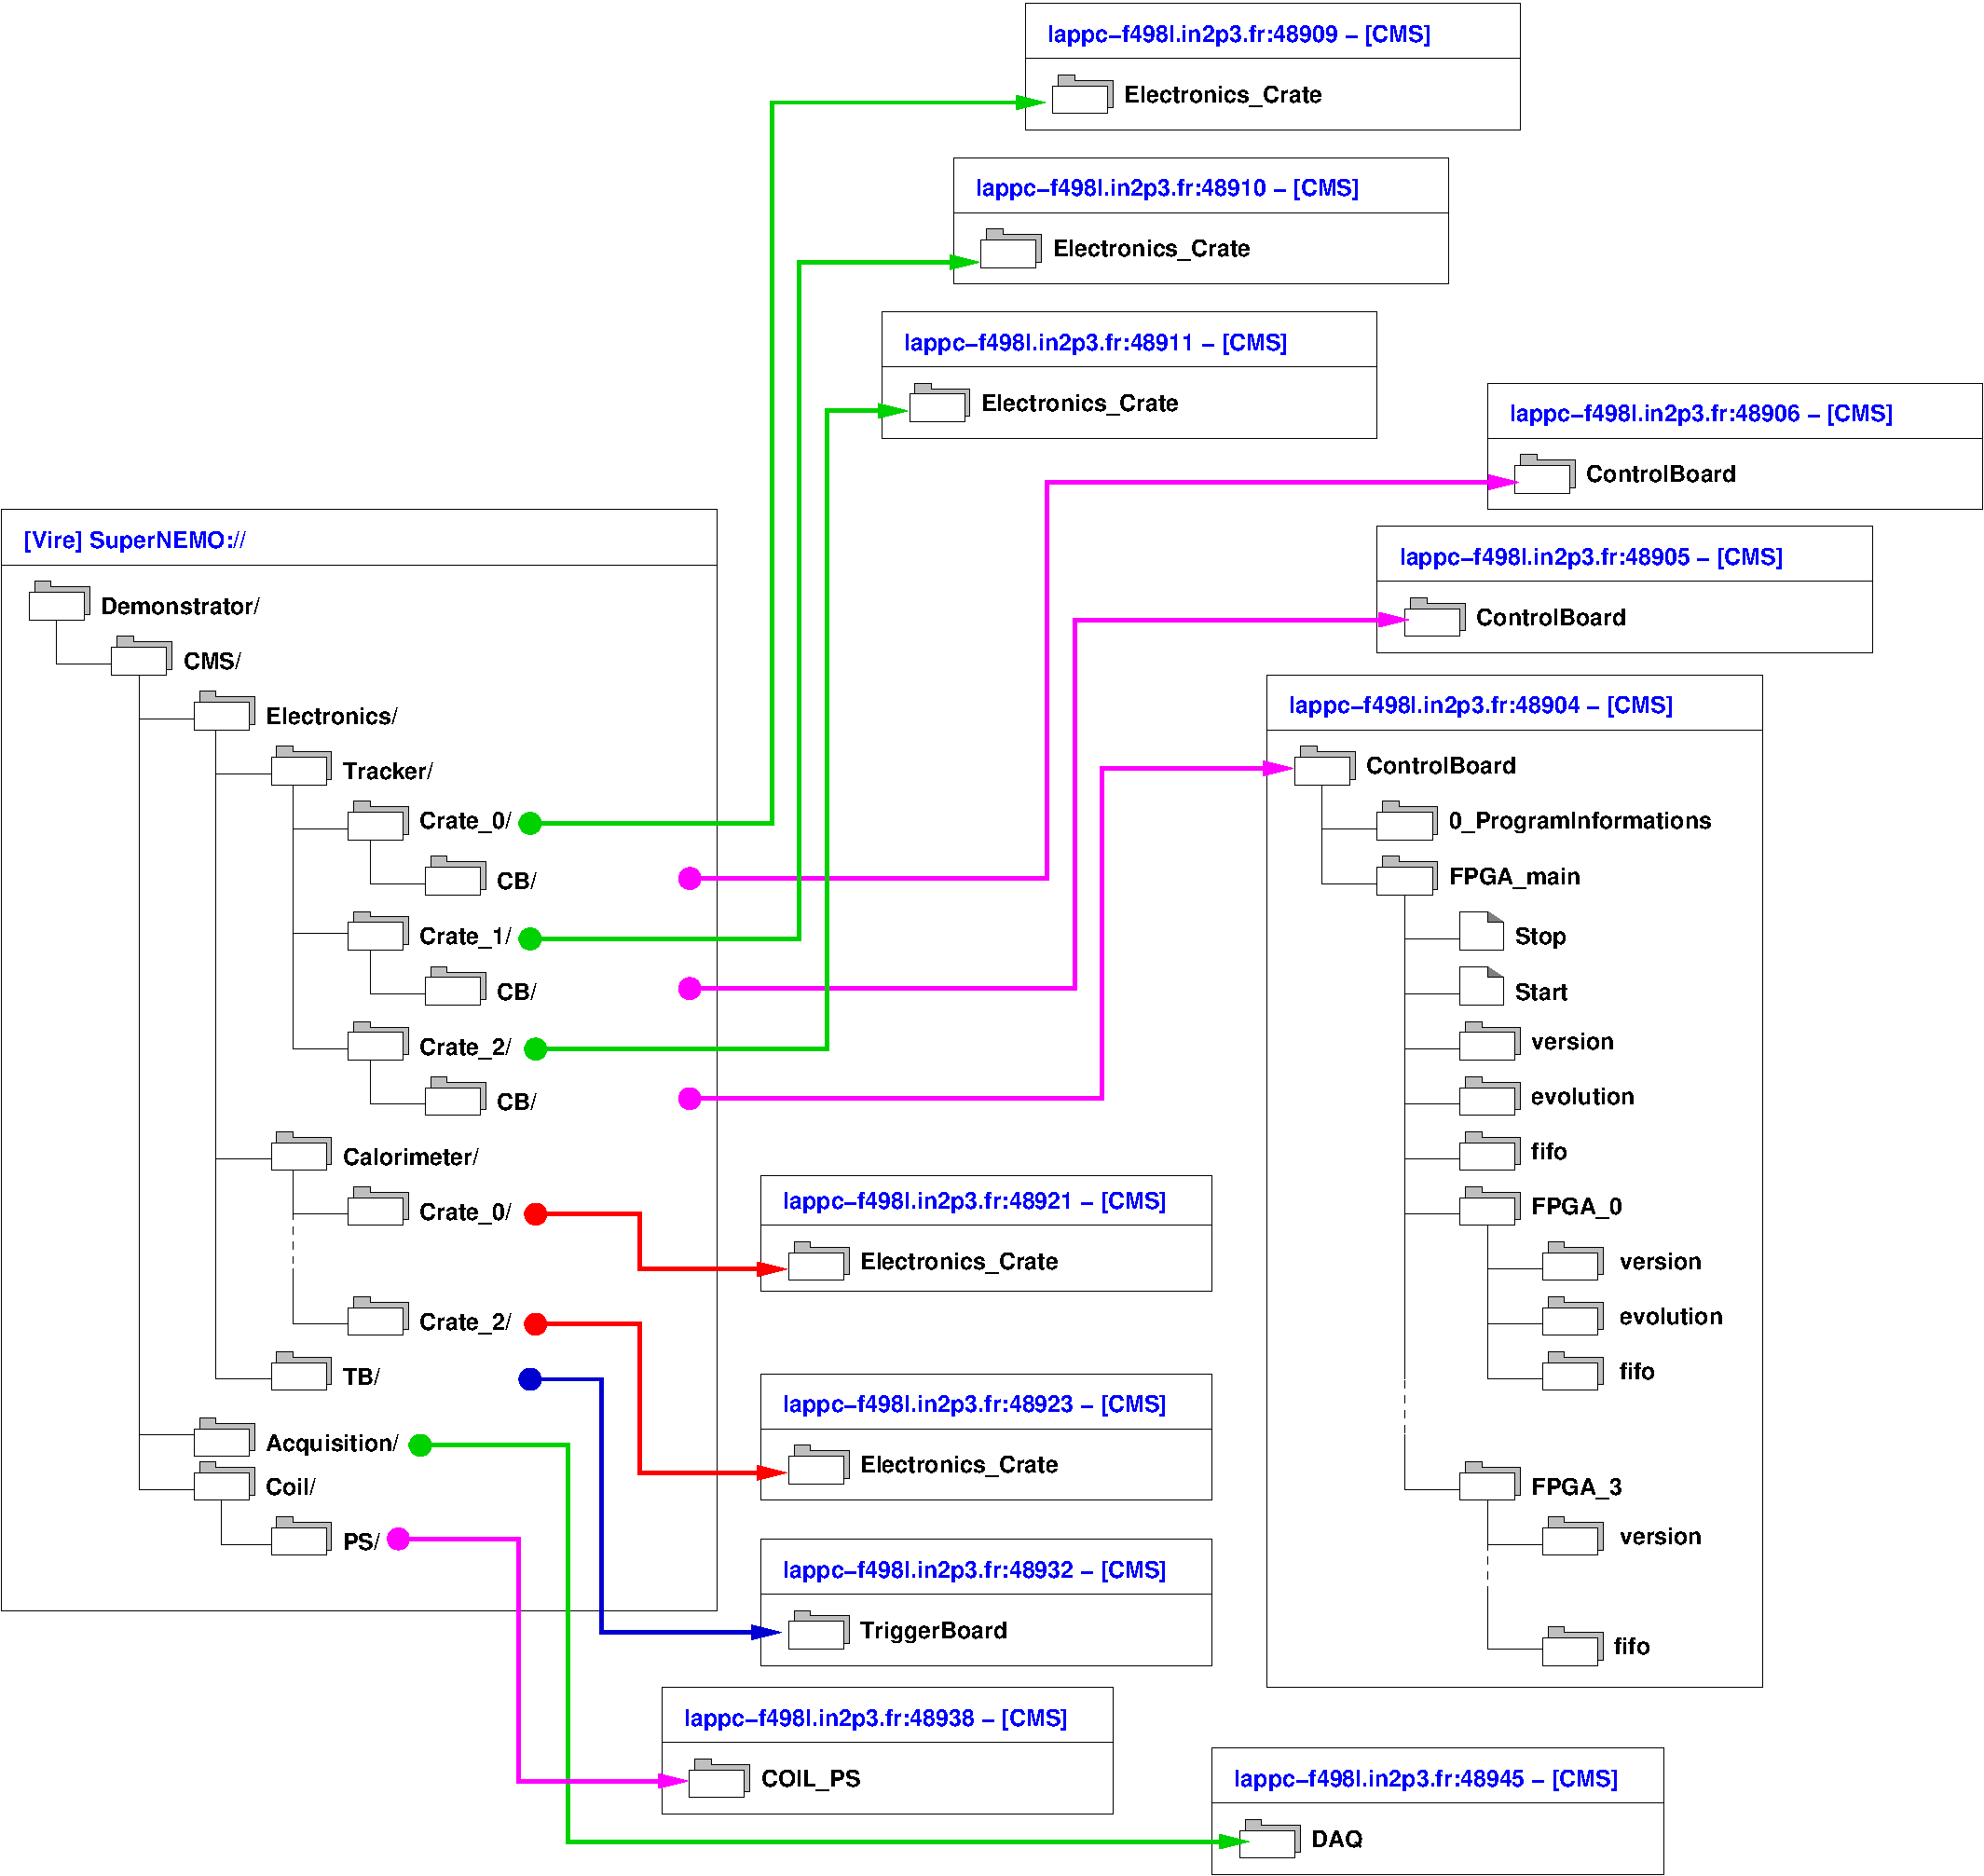
\includegraphics[width=\linewidth]{appendix/images/MOS_device_example_0.pdf}
\end{center}
\caption{The  mounting of  many  MOS device  hierarchies  in the  Vire
  device hierarchy.  Each OPCUA server  runs a simple  hardware device
  that is \emph{mounted} from a specific node with its own path.
%% of  devices described by the Vire API.
%%   The root device is named  \texttt{SuperNEMO:}.  The top level (root)
%%   device is  named \texttt{Demonstrator}. The devices  colored in blue
%%   are managed  through MOS/OPCUA. The  devices colored in  magenta are
%%   directly embedded in the Vire server.  Devices with the \texttt{dev}
%%   tag are typical  hardware device. Devices with  the \texttt{bot} tag
%%   are typical software devices.
}\label{fig:an:mos_dev_0}
\end{figure}




\subsection{Example}

Using  the examples  displayed  in  figure \ref{fig:an:mos_dev_0},  we
consider  in detail  the way  one specific  device managed  by MOS  is
mounted   in  the   Vire   hierarchy.  Figure   \ref{fig:an:mos_dev_3}
illustrates the mounting of a MOS device in Vire.

Here the Vire  server publishes the path of a  device representing the
control board  of the third  electronic crate  for the tracker  of the
SuperNEMO demonstrator module.  The full Vire path of this device is:

\textcolor{blue}{\texttt{SuperNEMO://Demonstrator/CMS/Electronics/Tracker/Crate\_2/CB}}

This is  the only Vire identifier  recognized by user to  address this
device.

On    the   figure,    one    can   see    that    the   MOS    server
\texttt{lappc−f498l.in2p3.fr} (port 48904) hosts a simple device which
is locally named \texttt{ControlBoard}.

When  mounting   this  device  in   the  Vire  hierarchy,   the  local
\texttt{[CMS]}  namespace and  \texttt{ControlBoard} device  names are
hidden and replaced by the Vire device path.  All daughter devices and
datapoints of  the \texttt{CMS/ControlBoard} device are  integrated as
daughters        of        the         Vire        device        named\\
\texttt{SuperNEMO://Demonstrator/CMS/Electronics/Tracker/Crate\_2/CB}.


For example, the \texttt{FPGA\_main} daughter device is now associated
to the following Vire path:

\textcolor{blue}{\texttt{SuperNEMO://Demonstrator/CMS/Electronics/Tracker/Crate\_2/CB/FPGA\_main/}}

and  its  \texttt{Stop} method  is  automatically  addressed with  the
following \emph{leaf} path:

\textcolor{blue}{\texttt{SuperNEMO://Demonstrator/CMS/Electronics/Tracker/Crate\_2/CB/FPGA\_main/Stop}}


\begin{figure}[h]
\begin{center}
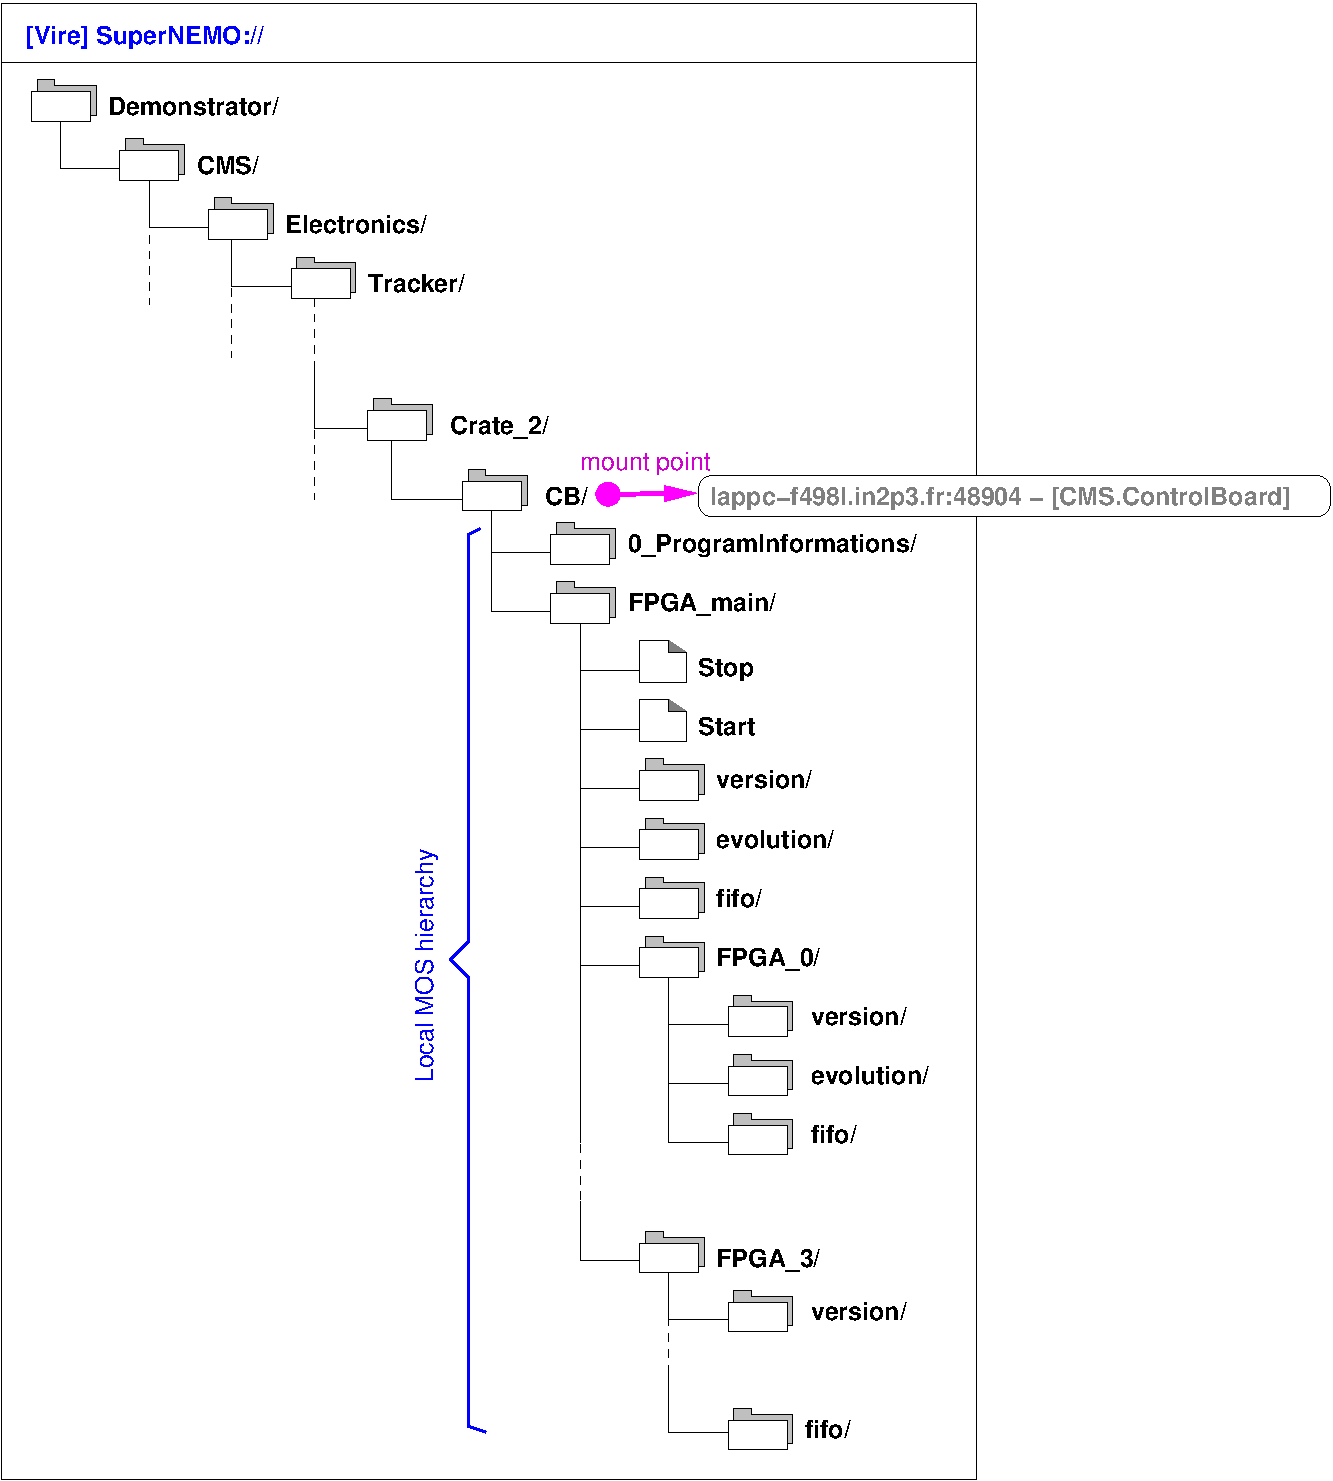
\includegraphics[width=0.8\linewidth]{appendix/images/MOS_device_example_3.pdf}
\end{center}
\caption{The  mounting of  one  MOS device and its local hierarchy  in the  Vire
  device hierarchy.}\label{fig:an:mos_dev_3}
\end{figure}



\subsection{Vire/MOS mapping}

As it can be  seen in the above example, the integration  of a new MOS
device in the Vire system is  achieved through soem kind of filesystem
mounting operation.   Particularly, it is  shown that the MOS  name of
the   mounted  root   device  is   replaced  by   an  arbitrary   Vire
path. However, all daughter  nodes (devices, datapoints) attached from
this root  node have their  relative MOS  names preserved in  the Vire
naming scheme.

Any  resource  (method)  associated  to any  of  such  daughter  nodes
inherits this relative naming scheme.

As Vire applications  describe resources through their  Vire paths, it
is thus needed to build an explicit map that associates resource paths
to MOS address  and name. The CMS  server will be able  to resolve the
MOS server/port and  embedded device associated to  the resource path.

The goal of the \texttt{devices\_launch.conf} file is not only to tell
the CMS server what MOS server should  be loaded and ran at start, but
also  to describe  the  \emph{mounting point/names}  used  by Vire  to
access the resources associated to MOS devices.  From the informations
stored in the  file, an explicit associative array must  be built when
the Vire server connect to the CMS server.  It will play the role of a
resource path resolver  when requests about resources will  be sent by
Vire applications.  This associative array  must be locked  during the
Vire/CMS connection.



%\subsubsection{Preparation of XML device models}

%% \noindent\underline{Pre-condition:}
%% The device is working and validated through the MOS/OPCUA server

%% \begin{enumerate}

%% \item Produce XML décrivant le modèle du device enrichi
%%   des metadata
%% Rédaction du fichier XML décrivant le modèle du device

%% \item Génération des fichiers model du type de device pour Vire

%% \item Génération des fichiers instances resolv.conf

%% \end{enumerate}


\vfill
\pagebreak
\clearpage

% end


\section{Vire messages}\label{app:vire_messages}

Within Vire  and between Vire  components and external  components, we
use  a communication  system  based on  Vire  messages.  This  section
describes the structure of such messages.

\subsection{General structure of a message}

Each message consists in two parts (figure \ref{fig-vire-message-message-cpp}):
\begin{itemize}

\item  the  \emph{header}  is   dedicated  to  generic  and  typicalle
  mandatory  informations  which  document   the  message  itself  and
  arbitrary high-level metadata.

\item  the \emph{body}  of the  message  contains the  real data: the payload.
  The structure of the message body depends on some convention. Vire uses
  its own convention to embed the payload data.

\end{itemize}

\begin{figure}[h]
\vskip 10pt
\small
\begin{Verbatim}[frame=single,xleftmargin=0.cm,label=\fbox{C++}]
struct vire::message::message {
  message_header header; // Header of the message
  message_body   body;   // Body of the message
};
\end{Verbatim}
\normalsize
\caption{The structure of a Vire message object (C++  class:
  \texttt{"vire::message::message"})}\label{fig-vire-message-message-cpp}
\end{figure}

\subsection{The message header}

The header contains (figure \ref{fig-vire-message-message_header-cpp}):
\begin{itemize}

  \item The mandatory \texttt{message\_id}  attribute is an identifier
    of the  message which  document the emitter  and a  unique message
    number.   Each emitter  is  responsible of  the  numbering of  the
    messages it  emits, typically using an  incremental technique. The
    message  number is  a positive  integer, starting  from 0  (figure
    \ref{fig-vire-message-message_identifier-cpp}).

  \item  The \texttt{timestamp}  attribute  encodes the  approximative
    time point when the message was  created. It contains the date and
    the time, using at least microsecond resolution.

    Typically,  with  JSON  encoding  system, it  is  expected  to  be
    formatted as a character string, using the following ISO format:

    \begin{center}
      \texttt{yyyymmddThhmmss.uuuuuu}
    \end{center}

    \noindent where:

    \vskip -10pt
    \begin{itemize}
    \item[\texttt{yyyymmdd} :] encodes year/month/day,
    \item[\texttt{hhmmssd} :] encodes hour/minute/second,
    \item[\texttt{uuuuuu} :] encodes microseconds.
    \end{itemize}

  \item   In   the   case    of   a   \emph{response}   message,   the
    \texttt{in\_reply\_to} attribute is set to identify the associated
    request message.

  \item  The \texttt{asynchronous}  boolean  attribute is  set if  the
    message processing  is explicitely requested  by the source  to be
    asynchronous (non-blocking).  In  RPC transactions, where requests
    are transmitted from one point to  the other, its default value is
    \emph{false}.   It  is possible  to  force  a RPC  transaction  in
    asynchronous mode.   This use  case is documented  elsewhere.  For
    event messaging, this flag is conventionally set to \emph{true}.

  \item  The  \texttt{body\_layout\_id}  attribute  is  the  mandatory
    identifier   of   the   layout   of  the   message   body   (class
    \texttt{"vire::utility::model\_identifier"}).  The  default layout
    for     message     body     inside    the     Vire     API     is
    \texttt{"vire::message::body\_format::typed\_payload"}, with version
    \texttt{"1.0"}                                             (figure
    \ref{fig-vire-utility-model_identifier-cpp}).

\end{itemize}


\begin{figure}[h]
\vskip 10pt
\small
\begin{Verbatim}[frame=single,xleftmargin=0.cm,label=\fbox{C++}]
struct vire::message::message_header {
  message_identifier message_id;     // Message identifier from the emitter.
  std::string        timestamp;      // Timestamp.
  message_identifier in_reply_to;    // Message identifier of the associated
                                     // request message (optional).
  bool               asynchronous,   // Asynchronous flag.
  vire::utility::model_identifier     body_layout_id; // Body layout identifier.
  std::map<std::string, std::string>  metadata;       // Key/value metadata dictionary.
};
\end{Verbatim}
\normalsize
\caption{The  structure  of  a   message  header  object  (C++  class:
  \texttt{"vire::message::message\_header"}).}\label{fig-vire-message-message_header-cpp}
\end{figure}

\begin{figure}[h]
\vskip 10pt
\small
\begin{Verbatim}[frame=single,xleftmargin=0.cm,label=\fbox{C++}]
struct vire::message::message_identifier {
  std::string emitter; // Name identifying the emitter of the message.
  int32_t     number;  // Number identifying the message in the emitter's
                       // message numbering scheme.
};
\end{Verbatim}
\normalsize
\caption{The      structure      of     a      message      identifier
  (C++  class:  \texttt{"vire::message::message\_identifier"}).}
\label{fig-vire-message-message_identifier-cpp}
\end{figure}

\begin{figure}[h]
\vskip 10pt
\small
\begin{Verbatim}[frame=single,xleftmargin=0.cm,label=\fbox{C++}]
struct vire::utility::model_identifier {
  std::string name;    // Name identifying the format of the message.
  std::string version; // String identifying the version of the format.
};
\end{Verbatim}
\normalsize
\caption{The structure of a model identifier (C++  class:  \texttt{"vire::utility::model\_identifier"}.}\label{fig-vire-utility-model_identifier-cpp}
\end{figure}




\begin{figure}[h]
\vskip 10pt
\small
\begin{Verbatim}[frame=single,xleftmargin=0.cm,label=\fbox{JSON}]
{
   "header" : {
      "message_id" : {
         "emitter" : "vire.server",
         "number" : 42
      },
      "timestamp" : "20160930T141408.413443",
      "in_reply_to" : {
         "initialized" : true,
         "value" : {
            "emitter" : "vire.client.0",
            "number" : 23
         }
      },
      "asynchronous" : false,
      "body_layout_id" : {
         "name" : "vire::message::body_format::typed_payload",
         "version" : {
            "initialized" : true,
            "value" : "1.0"
         }
      },
      "metadata" : [
         {
            "key" : "key1",
            "value" : "foo"
         },
         {
            "key" : "key2",
            "value" : "42"
         },
         {
            "key" : "key3",
            "value" : "3.1415899999999999"
         },
         {
            "key" : "key4",
            "value" : "true"
         }
      ]
   }
  "body" : {
      ...
   }
}
\end{Verbatim}
\normalsize
\caption{Example of  a   message  header  object in JSON format.}
\label{fig-vire-message-message_header-json}
\end{figure}

\vfill
\clearpage
\pagebreak

\subsection{The message body}

The    default    message   body    layout    in    Vire   is    named
\texttt{"vire::message::body\_format::typed\_payload"}        (version
\texttt{"1.0"}).   Each  message used  within  the  Vire framework  is
supposed to use this layout.  The general idea is that the body of the
message embeded the  \emph{payload object} that has  to be transmitted
between  two components  of  the system.   \emph{Payload objects}  are
classified in one of the three following categories:

\begin{enumerate}

\item \emph{Request}:  describes a request submitted  by one component
  to another component (generally during a synchronous RPC transaction).

\item  \emph{Response}: describes  the  response to  a former  request
  (generally during a synchronous RPC transaction).

\item \emph{Event}: describes an  arbitrary information record (alarm,
  exception, signal\dots) which is transmitted asynchronously.

\end{enumerate}

Vire implements the following class hierarchy:

\begin{center}
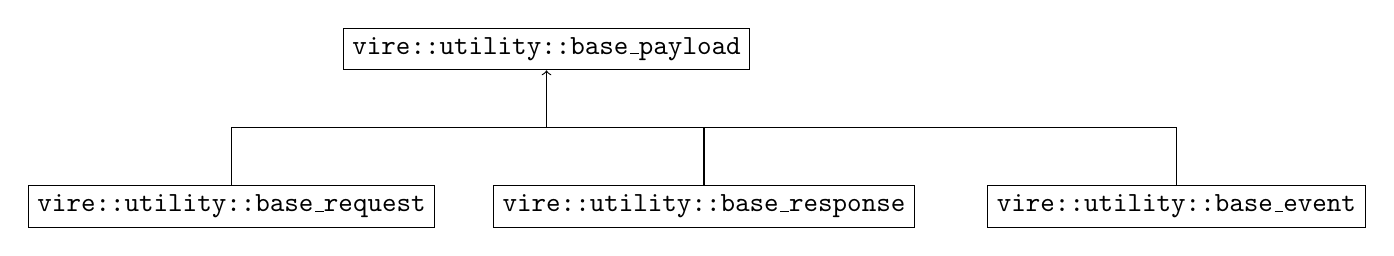
\begin{tikzpicture}
  \node (payload)  at (0,2)  [draw] {\texttt{vire::utility::base\_payload}};
  \node (request)  at (-4,0) [draw] {\texttt{vire::utility::base\_request}};
  \node (response) at (2,0)  [draw] {\texttt{vire::utility::base\_response}};
  \node (event)    at (8,0)  [draw] {\texttt{vire::utility::base\_event}};

  %\draw[style=help lines] (-3,-1) grid (10,4);
  \draw (node cs:name=response,anchor=north) |- (0,1);
  \draw (node cs:name=event,anchor=north)    |- (0,1);
  \draw[->] (node cs:name=request,anchor=north)
  |- (0,1) -| (node cs:name=payload,anchor=south);
\end{tikzpicture}
\end{center}

The requirements for the transmitted object are the following:

\begin{itemize}

\item The  type of the object  must be conventionally associated  to a
  unique     \emph{model      identifier}     object      (see     the
  \texttt{"vire::utility::model\_identifier"} class)  which contains a
  unique   name   (\textit{string    identifier})   and   possibly   a
  \textit{version identifier}.  Each software  component that may send
  or  receive the  object  should agree  on  this type  identification
  scheme.   This   enable  the  use  of   object  factories,  whatever
  programming  langage  is used  on  both  side of  the  communication
  system.

\item  For each  software component,  the object  type must  have some
  dedicated  encoding/decoding  functions  available  (again  whatever
  programming language is used). For example the Vire API supports the
  following encoding formats:

  \begin{itemize}

  \item JSON (MIME  encoding type: \texttt{"application/x-json"}), which
    is supportable by many languages,

  \item  Protobuf  (Google  Protocol   Buffers,  MIME  encoding  type:
    \texttt{"application/x-protobuf"}), which is also widely supported,

  \item   Boost/serialisation   (XML,    text   or   binary   archives
    \texttt{"application/x-boost-serialization-xml"},
    \texttt{"application/x-boost-serialization-text"},
    \texttt{"application/x-boost-serialization-binary"}),    which    in
    principle is supported by C++ only.

  \end{itemize}

  The Protobuf  encoding format will be  used to serialize/deserialize
  the  Vire  messages transported  between  the  Vire server  and  the
  CMS/LAPP server.

\end{itemize}

Vire uses a dedicated layout to represent the body of any message with
its embedded payload object. With this technique, the structure of the
body          contains         two          attributes         (figure
\ref{fig-app-vire-message-message_body-cpp}):

\begin{enumerate}

\item The \texttt{payload\_type\_id} specifies the type of the payload
  object   (figure   \ref{fig-app-vire-utility-model_identifier-cpp}).
  This unique name  is conventionaly fixed for a  given application. A
  version tag allows to support possible evolution of the object type.

\item The  \texttt{payload} is a  handle to  a payload object  of type
  request, response or event.

  %% \begin{itemize}
  %% \item Within  the producer  component of  the message,  the encoding
  %%   function associated to the object  type is responsible to generate
  %%   the JSON stream for the object and store it in the buffer.

  %% \item Within  the consumer  component of  the message,  the decoding
  %%   function associated to the object type is responsible to parse the
  %%   JSON stream stored in the buffer and restore the object in memory.

  %% \end{itemize}

  It is expected  that, on both sides of the  connection, the software
  components can  access dedicated  software plugins which  ensure the
  support  of  various   \emph{payload  object  types}  conventionnaly
  associated  with  their  \emph{payload type  identifiers}  and  also
  providing JSON and/or Protobuf encoding/decoding functionalities.

  %% The   system  allows  to  support
  %% modification  in the  structure of  the objects  thanks to  version
  %% tagging.

\end{enumerate}

\begin{figure}[h]
\vskip 10pt
\small
\begin{Verbatim}[frame=single,xleftmargin=0.cm,label=\fbox{C++}]
struct message_body {
  vire::utility::model_identifier     payload_type_id; // Object type identifier.
  const vire::utility::base_payload * payload;         // Handle to a payload object.
};
\end{Verbatim}
\normalsize
\caption{The structure of a message body object (C++).}
\label{fig-app-vire-message-message_body-cpp}
\end{figure}

\begin{figure}[h]
\vskip 10pt
\small
\begin{Verbatim}[frame=single,xleftmargin=0.cm,label=\fbox{JSON}]
{
  "header" : {
    ...
  },
  "body" : {
    "payload_type_id" : {
      "name" : "vire::message::testing::error_event",
      "version" : {
        "initialized" : false
      }
    },
    "payload" : {
      "timestamp" : "20160930T141743.759085"
      "err" : {
        "code" : 3,
        "message" : "A basic error"
      },
    }
  }
}
\end{Verbatim}
\normalsize
\caption{Example of  a   message  body  object in JSON format.}
\label{fig-vire-message-message_body-json}
\end{figure}

\vfill
\clearpage
\pagebreak

% end

%\input{appendix/app_json_fmt.tex}

\section{The \emph{Protocol Buffers} format}\label{app:protobuf_fmt}

\subsection{Introduction}

The  Google  Protocol Buffers  (\emph{protobuf})  library  is used  to
represent the objects that are exchanged between the Vire clients, the
Vire server and the CMS server.  The  version 3 of the format is used,
implying   at   least   version   3.0.0  (September   2016)   of   the
\emph{protobuf} library.

Each  data   structure  of  interest   can  be  described   through  a
\texttt{.proto}  file  from  which  stub files  can  be  automatically
generated  with the  \texttt{protoc} compiler.  For Vire  and its  CMS
interface, the C++ and Java programming languages will be used.


A  collection of  \texttt{.proto}  files are  provided  with the  Vire
library to represent all kind  of data structures transferable between
networked agents  (Vire server,  Vire clients, CMS/LAPP  server).  The
objects of  the highest level  are named \emph{payload  objects} (like
\emph{request},  \emph{response} and  \emph{event} objects).   They
are composed of attributes of more basic data structures.

\subsection{Example}

The following  class diagram  illustrates two data  structures defined
within the Vire library with an inheritance relationship between them.

\begin{center}
  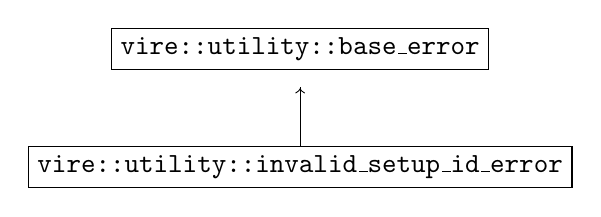
\begin{tikzpicture}
    \node (base)     at (0,1.5)  [draw] {\texttt{vire::utility::base\_error}};
    \node (setup)    at (0,0)  [draw] {\texttt{vire::utility::invalid\_setup\_id\_error}};

    \draw[->]   (node cs:name=setup,anchor=north) |- (0,1);
    |- (0,1) -| (node cs:name=base,anchor=south);
  \end{tikzpicture}
\end{center}

The \texttt{vire::utility::base\_error}  is the  parent class  for all
\emph{error}  objects.   It  contains   two  attributes:   an  integer
\emph{error code}  and a  character string describing  the \emph{error
  message}.

The   \texttt{vire::utility::invalid\_setup\_id\_error}  class   is  a
specialized error class  which represents explicitely an  error due to
an identification  failure of  the experimental setup.   It implements
additional mutually exclusive attributes: the \emph{unrecognized name}
of the setup or the \emph{unrecognized version} of the setup.

This   example  illustrates   the  protobuf   representation  of   the
\texttt{vire::utility::base\_error}  in the  Vire  library, using  the
\texttt{"vire/utility/BaseError.proto"} file:

\small
\begin{Verbatim}[frame=single,xleftmargin=0.cm,label=\fbox{protobuf}]
  syntax = "proto3";
  package vire.utility; // Namespace

  message BaseError {

    // reserved 1; // Reserved for _base message

    // Attributes:
    int32  code           = 100; // The error code
    string message_format = 101; // The error description message

  }
\end{Verbatim}
\normalsize

\vfill
\clearpage
\pagebreak

\subsection{Vire protobuf conventions}

Vire uses the following conventions:

\begin{enumerate}

\item
  The member index  \texttt{1} is reserved to represent the  link of a
  class to its main base/parent class (if any).  It is not used if the
  data structure does not inherit any data structure.
  If a data structure naturally inherits another one, it is thus possible
  to  represent the  inheritance  relationship as  illustrated with  the
  \texttt{"vire/utility/InvalidSetupIdError.proto"}      file      which
  represents the \texttt{vire::utility::invalid\_setup\_id\_error} class
  in the Vire library:

  \small
  \begin{Verbatim}[frame=single,xleftmargin=0.cm,label=\fbox{protobuf}]
    syntax = "proto3";
    package vire.utility; // Namespace

    import "vire/utility/BaseError.proto"; // Dependency

    message InvalidSetupIdError {

      BaseError _base = 1; // The base class

      // Additional attributes:
      oneof detail { // Mutual exclusion
        string invalid_setup_name    = 100; // The failed setup name
        string invalid_setup_version = 101; // The failed setup version
      }

    }
  \end{Verbatim}
  \normalsize

\item The  \texttt{\_base} member  is conventionally  used to  represent the
  inheritance   relationship    from   a   data   structure    of   type
  \texttt{"vire.utility.BaseError"}.

\item Member indexes from \texttt{2}  to \texttt{99} are also reserved
  for possible future usage (multiple inheritance, metadata\dots).

\item
  The first member of the data structure must start at index \texttt{100}.

\end{enumerate}

\vfill
\clearpage
\pagebreak

% end


\section{Vire payload objects}\label{app:payload}

\subsection{Introduction}

As  mentioned in  appendix \ref{app:protobuf_fmt},  Vire messages  are
wrappers for \emph{payload objects}.  Each  type of payload object can
be represented  through the \emph{protobuf} mechanism.   The following
class hierarchy shows the base architecture used to define new payload
objects.

\begin{center}
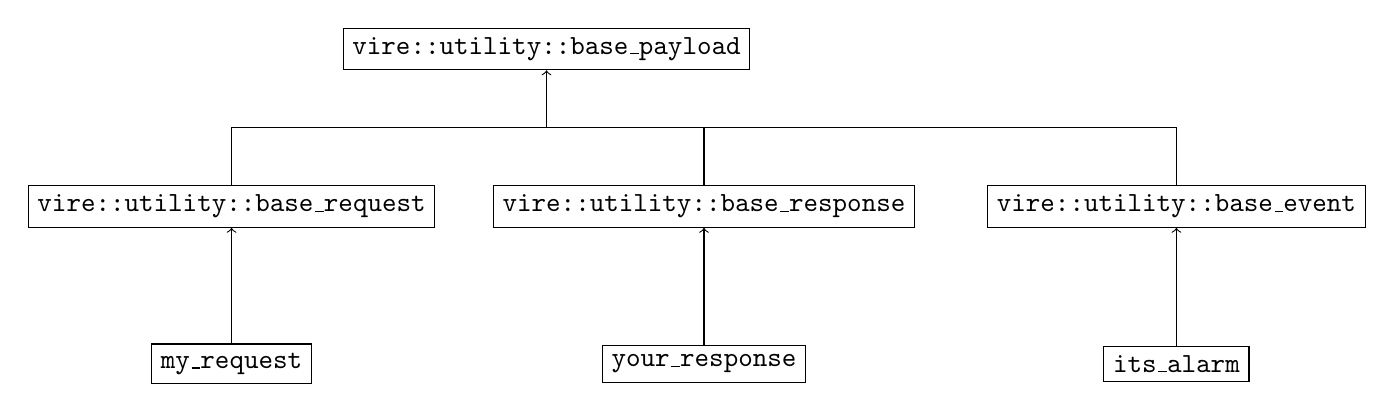
\begin{tikzpicture}
  \node (payload)  at (0,2)   [draw] {\texttt{vire::utility::base\_payload}};
  \node (request)  at (-4,0)  [draw] {\texttt{vire::utility::base\_request}};
  \node (response) at (2,0)   [draw] {\texttt{vire::utility::base\_response}};
  \node (event)    at (8,0)   [draw] {\texttt{vire::utility::base\_event}};
  \node (my)       at (-4,-2) [draw] {\texttt{my\_request}};
  \node (your)     at (2,-2)  [draw] {\texttt{your\_response}};
  \node (its)    at (8,-2)    [draw] {\texttt{its\_alarm}};

  %\draw[style=help lines] (-6,-2) grid (10,2);
  \draw (node cs:name=response,anchor=north) |- (0,1);
  \draw (node cs:name=event,anchor=north)    |- (0,1);
  \draw[->] (node cs:name=request,anchor=north)
  |- (0,1) -| (node cs:name=payload,anchor=south);
  \draw[->] (node cs:name=my,anchor=north)
  |- (-4,-1) -| (node cs:name=request,anchor=south);
  \draw[->] (node cs:name=your,anchor=north)
  |- (2,-1) -| (node cs:name=response,anchor=south);
  \draw[->] (node cs:name=its,anchor=north)
  |- (8,-1) -| (node cs:name=event,anchor=south);
\end{tikzpicture}
\end{center}


\begin{center}
\vskip 10pt
\small
\begin{tabular}{|l|l|l|}
  \hline
  \textbf{Vire C++ class} & \textbf{protobuf message type} & \textbf{protobuf definition file} \\
  \hline
  \hline
  \multicolumn{3}{|c|}{\emph{general types}} \\
  \hline
  boost::posix\_time::ptime & google.protobuf.Timestamp & google/protobuf/timestamp.proto \\
  \hline
  \hline
  \multicolumn{3}{|c|}{\emph{identifier types}} \\
  \hline
  vire::utility::base\_identifier & vire.utility.Baseidentifier & vire/utility/Baseidentifier.proto \\
  \hline
  vire::utility::instance\_identifier & vire.utility.InstanceIdentifier & vire/utility/InstanceIdentifier.proto \\
  \hline
  vire::utility::model\_identifier & vire.utility.ModelIdentifier & vire/utility/ModelIdentifier.proto \\
  \hline
  \hline
  \multicolumn{3}{|c|}{\emph{error types}} \\
  \hline
  vire::utility::base\_error & vire.utility.BaseError & vire/utility/BaseError.proto \\
  \hline
  vire::utility::invalid\_context\_error & vire.utility.InvalidContextError & vire/utility/InvalidContextError.proto \\
  \hline
  vire::utility::invalid\_setup\_id\_error & vire.utility.InvalidSetupIdError & vire/utility/InvalidSetupIdError.proto \\
  \hline
  \hline
  \multicolumn{3}{|c|}{\emph{payload types}} \\
  \hline
  vire::utility::base\_payload & vire.utility.BasePayload & vire/utility/BasePayload.proto \\
  \hline
  vire::utility::base\_request & vire.utility.BaseRequest & vire/utility/BaseRequest.proto \\
  \hline
  vire::utility::base\_response & vire.utility.BaseResponse & vire/utility/BaseResponse.proto \\
  \hline
  vire::utility::base\_event & vire.utility.BaseEvent & vire/utility/BaseEvent.proto \\
  \hline
  vire::utility::base\_alarm & vire.utility.BaseAlarm & vire/utility/BaseAlarm.proto \\
  \hline
  \hline
  \multicolumn{3}{|c|}{\emph{messenging types}} \\
  \hline
  vire::message::message\_identifier & vire.message.MessageIdentifier & vire/message/MessageIdentifier.proto \\
  \hline
  vire::message::msg\_header & vire.message.MsgHeader & vire/message/MsgHeader.proto \\
  \hline
  vire::message::msg\_body & vire.message.MsgBody & vire/message/MsgBody.proto \\
  \hline
  vire::message::message & vire.message.Message & vire/message/Message.proto \\
  \hline
\end{tabular}
\normalsize
\end{center}


\begin{center}
\vskip 10pt
\small
\begin{tabular}{|l|l|l|}
  \hline
  \multicolumn{3}{|c|}{\emph{Resource management related types}} \\
  \hline
  vire::cms::resource\_status\_record & vire.cms.ResourceStatusRecord & vire/cms/ResourceStatusRecord.proto \\
  \hline
  vire::cms::resource\_fetch\_status\_request & vire.cms.ResourceFetchStatusRequest & vire/cms/ResourceFetchStatusRequest.proto \\
  \hline
  vire::cms::resource\_fetch\_status\_success\_response & vire.cms.ResourceFetchStatusSuccessResponse & vire/cms/ResourceFetchStatusSuccessResponse.proto \\
  \hline
  vire::cms::resource\_fetch\_status\_failure\_response & vire.cms.ResourceFetchStatusFailureResponse & vire/cms/ResourceFetchStatusFailureResponse.proto \\
  \hline
  vire::cms::resource\_exec\_request & vire.cms.ResourceExecRequest & vire/cms/ResourceExecRequest.proto \\
  \hline
  vire::cms::resource\_exec\_success\_response & vire.cms.ResourceExecSuccessResponse & vire/cms/ResourceExecSuccessResponse.proto \\
  \hline
  vire::cms::resource\_exec\_failure\_response & vire.cms.ResourceExecFailureResponse & vire/cms/ResourceExecFailureResponse.proto \\
  \hline
  vire::cms::resource\_exec\_non\_blocking\_request & vire.cms.ResourceExecNonBlockingRequest & vire/cms/ResourceExecNonBlockingRequest.proto \\
  \hline
  vire::cms::resource\_exec\_non\_blocking\_ack\_response & vire.cms.ResourceExecNonBlockingAckResponse & vire/cms/ResourceExecNonBlockingAckResponse.proto \\
  \hline
  vire::cms::resource\_exec\_non\_blocking\_noack\_response & vire.cms.ResourceExecNonBlockingNoackResponse & vire/cms/ResourceExecNonBlockingNoackResponse.proto \\
  \hline
  vire::cms::resource\_exec\_non\_blocking\_success\_event & vire.cms.ResourceExecNonBlockingSuccessEvent & vire/cms/ResourceExecNonBlockingSuccessEvent.proto \\
  \hline
  vire::cms::resource\_exec\_non\_blocking\_failure\_event & vire.cms.ResourceExecNonBlockingFailureEvent & vire/cms/ResourceExecNonBlockingFailureEvent.proto \\
  \hline
  vire::cms::resource\_exec\_error & vire.cms.ResourceExecError & vire/cms/ResourceExecError.proto \\
  \hline
  vire::cms::invalid\_status\_error & vire.cms.ResourceExecError & vire/cms/ResourceExecError.proto \\
  \hline
  %% vire::cms::invalid\_credentials\_error & vire.cms.InvalidCredentialsError & vire/cms/InvalidCredentialsError.proto \\
  %% \hline
  %% vire::cms::invalid\_user\_error & vire.cms.InvalidUserError & vire/cms/InvalidUserError.proto \\
  %% \hline
  vire::cms::invalid\_resource\_error & vire.cms.InvalidUserError & vire/cms/InvalidUserError.proto \\
  \hline
  vire::cms::no\_pubsub\_resource\_error & vire.cms.NoPubsubResourceError & vire/cms/NoPubsubResourceError.proto \\
  \hline
  \hline
  \multicolumn{3}{|c|}{\emph{Resource pub/sub management types}} \\
  \hline
  vire::cms::resource\_pubsub\_subscribe\_request & vire.cms.ResourcePubsubSubscribeRequest & vire/cms/ResourcePubsubSubscribeRequest.proto \\
  \hline
  vire::cms::resource\_pubsub\_subscribe\_success\_response & vire.cms.ResourcePubsubSubscribeRSuccessResponse & vire/cms/ResourcePubsubSubscribeRSuccessResponse.proto \\
  \hline
  vire::cms::resource\_pubsub\_subscribe\_failure\_response & vire.cms.ResourcePubsubSubscribeRFailureResponse & vire/cms/ResourcePubsubSubscribeRSuccessResponse.proto \\
  \hline
  \hline
  \multicolumn{3}{|c|}{\emph{Vire/CMS server interface types}} \\
  \hline
  vire::cmsinterface::connection\_request & vire.cmsinterface.ConnectionRequest & vire/cmsinterface/ConnectionRequest.proto \\
  \hline
  vire::cmsinterface::connection\_success\_response & vire.cmsinterface.ConnectionSuccessResponse & vire/cmsinterface/ConnectionSuccessResponse.proto \\
  \hline
  vire::cmsinterface::connection\_failure\_response & vire.cmsinterface.ConnectionFailureResponse & vire/cmsinterface/ConnectionFailureResponse.proto \\
  \emph{embedded:} unknown\_resources\_error & .UnknownResourcesError &  \\
  \hline
  vire::cmsinterface::disconnection\_request & vire.cmsinterface.DisconnectionRequest & vire/cmsinterface/DisconnectionRequest.proto \\
  \hline
  vire::cmsinterface::disconnection\_success\_response & vire.cmsinterface.DisconnectionSuccessResponse & vire/cmsinterface/DisconnectionSuccessResponse.proto \\
  \hline
  %% \hline
  %% vire::cmsinterface::disconnection\_failure\_response & vire.cmsinterface.DisconnectionFailureResponse & vire/cmsinterface/DisconnectionFailureResponse.proto \\
\end{tabular}
\normalsize
\end{center}

\subsection{Basic data structures}

Any  payload object  (request, response  or event)  generally contains
some information records which are  specific to the functionalities of
the  payload  object they  belong.   These  records are  of  arbitrary
types. Of course they should be  translatable in terms of the protobuf
library.
%Of course they can be (de)serialized using JSON.
Some of these types are very  general and defined within the Vire core
API itself because they are reused by various payload objects not only
through  the Vire-CMS/LAPP  interface  but also  between  Vire clients  and
servers, independently  of the  CMS/LAPP server.  However,  the use  of the
Protocol Buffers interface makes possible  to publish the interface of
such data to the outside world, including the CMS/LAPP server in priority.

%% Other one are specific to the Vire/CMS interface and thus managed only
%% in the \texttt{Vire\_CMSInterface} API.
These  types  are considered  as  \emph{basic}.  Among them  we  find:
generic error  types, generic  identifier types,  timestamps, resource
status records\dots We propose to describe them in this section.

Once a sufficient collection of  basic data record types is available,
it  is possible  to describe  high  level payload  object types  which
aggregate attributes of such types.

Other record  types are specific to  some payload objects and  will be
never  used outside  the scope  of these  payload objects.   Such data
structures will be  explicitely declared with the  payload object they
belong to, likely as embedded types/classes.


\subsubsection{Errors}

Some  \emph{response} or  \emph{event} payload  objects may  contain a
specific  error  record  object.   A  \emph{failure  response}  or  an
\emph{exception  event}  object will  generally  embed  such an  error
record object.

Each  \emph{error record}  is represented  by an  instance of  a given
error type.   Each of  the error  types defined  in Vire  inherits the
\texttt{vire::utility::base\_error}      base       class      (figure
\ref{fig-app-payload-base_error})   which   contains   the   following
attributes:

\begin{itemize}

\item the error code: A non zero  integer which is set to 1 by default
  (indicating  a  generic  failure  case).   The  error  code  can  be
  conventionally  set to  any positive  integer value  to represent  a
  specific error case, depending on the context.

\item the error  message: an optional human  readable character string
  which documents the error as usefully as possible.

\end{itemize}

\begin{figure}[h]
\vskip 10pt
\small
\begin{Verbatim}[frame=single,xleftmargin=0.cm,label=\fbox{C++}]
struct vire::utility::base_error
{
  // Attributes:
  int         code;           // Error code (>0).
  std::string message_format; // Error message (optional).
};
\end{Verbatim}
\normalsize
\caption{The structure of a \texttt{"vire::utility::base\_error"} object
  (C++).}
\label{fig-app-payload-base_error}
\end{figure}


%% An example of JSON formatted basic error object is given in figure
%% \ref{fig-app-payload-base_error-1}.
%%
%% \begin{figure}[h]
%% \vskip 10pt
%% \small
%% \begin{Verbatim}[frame=single,xleftmargin=0.cm,label=\fbox{\texttt{JSON}}]
%% {
%%   "code" : "42",
%%   "message_format" : "Invalid AMQP server port=[2341]"
%% }
%% \end{Verbatim}
%% \normalsize
%% \caption{JSON  formatted  basic  error  object  (class
%%   \texttt{vire::utility::base\_error}.}
%% \label{fig-app-payload-base_error-1}
%% \end{figure}

Several type of generic errors are defined in Vire:


\begin{center}
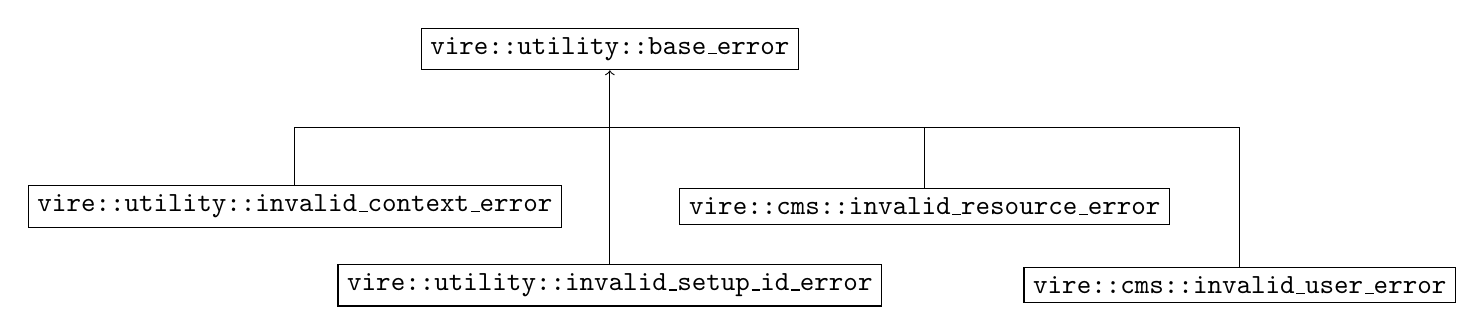
\begin{tikzpicture}
  \node (base)     at (0,2)  [draw] {\texttt{vire::utility::base\_error}};
  \node (context)  at (-4,0) [draw] {\texttt{vire::utility::invalid\_context\_error}};
  \node (setup)    at (0,-1)  [draw] {\texttt{vire::utility::invalid\_setup\_id\_error}};
  \node (resource) at (4,0)  [draw] {\texttt{vire::cms::invalid\_resource\_error}};
  \node (user)     at (8,-1)  [draw] {\texttt{vire::cms::invalid\_user\_error}};

  \draw     (node cs:name=setup,anchor=north)    |- (0,1);
  \draw     (node cs:name=resource,anchor=north) |- (0,1);
  \draw     (node cs:name=user,anchor=north)     |- (0,1);
  \draw[->] (node cs:name=context,anchor=north)
  |- (0,1) -| (node cs:name=base,anchor=south);
\end{tikzpicture}
\end{center}

\noindent
Here are a few error object types defined in Vire.  Some types belongs
to the \texttt{utility} namespace, other  ones are in the \texttt{cms}
namespace:

\begin{itemize}

\item \texttt{"vire::utility::invalid\_context\_error"} : occurs typically when
  the general context of the execution of a given resource is not adapted.\\
  It is mapped to the \texttt{"vire.utility.InvalidContextError"} protobuf record.

\item \texttt{"vire::utility::invalid\_setup\_id\_error"} : occurs in case
  of an invalid identification of the experimental setup managed
  by the Vire or CMS server.\\
  It is mapped to the \texttt{"vire.utility.InvalidSetupIdError"} protobuf record.

\item \texttt{"vire::cms::invalid\_resource\_error"} : occurs in case
  of an invalid identification of a resource.\\
  It is mapped to the  \texttt{"vire.cms.InvalidResourceError"} protobuf record.

\item \texttt{"vire::cms::invalid\_status\_error"}: occurs when an attempt
  to access a resource that has not the proper status.\\
  It is mapped to the  \texttt{"vire.cms.InvalidStatusError"} protobuf record.

\item \texttt{"vire::cms::invalid\_user\_error"} : occurs in case
  of an invalid identification of an user.\\
  It is mapped to the  \texttt{"vire.cms.InvalidUserError"} protobuf record.

\item \texttt{"vire::cms::invalid\_credentials\_error"} : occurs in case
  of user authentication error.\\
  It is mapped to the  \texttt{"vire.cms.InvalidCredentialsError"} protobuf record.

\item \texttt{"vire::cms::resource\_exec\_error"} : occurs in case
  of error at the execution of a given resource.\\
  It is mapped to the  \texttt{"vire.cms.ResourceExecError"} protobuf record.

\end{itemize}



\subsubsection{Object and type identifiers}

Vire  uses  some dedicated  classes  to  represent the  identifier  of
various objects  (or \emph{instances})  as well  as various  types (or
\emph{models})  of components.  Vire  implements  the following  class
hierarchy:

\begin{center}
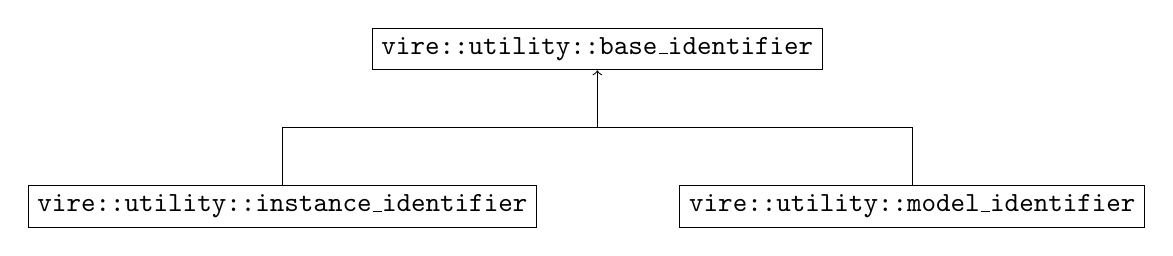
\begin{tikzpicture}
  \node (base)  at (0,2)  [draw] {\texttt{vire::utility::base\_identifier}};
  \node (instance)  at (-4,0) [draw] {\texttt{vire::utility::instance\_identifier}};
  \node (model) at (4,0)  [draw] {\texttt{vire::utility::model\_identifier}};

  \draw (node cs:name=model,anchor=north) |- (0,1);
\draw[->] (node cs:name=instance,anchor=north)
  |- (0,1) -| (node cs:name=base,anchor=south);
\end{tikzpicture}
\end{center}

The          \texttt{vire::utility::base\_identifier}          (figure
\ref{fig-app-payload-base_identifier}) class is  a pure abstract class
that cannot be instantiated. However  it contains a mandatory name and
an  optional  version description  which  are  used by  all  inherited
classes:

\begin{itemize}

\item The   \texttt{vire::utility::instance\_identifier}    concrete   class
inherits  \texttt{vire::utility::base\_identifier}  and   is  used  to
identify \underline{unique instances of objects} known by the system.

\item The  \texttt{vire::utility::model\_identifier}   concrete  class  also
inherits  \texttt{vire::utility::base\_identifier}  and   is  used  to
identify \underline{types of objects} registered in the system.

\end{itemize}

The only difference between these two classes is the validation scheme
of  the name  attribute.

\begin{figure}[h]
\vskip 10pt
\small
\begin{Verbatim}[frame=single,xleftmargin=0.cm,label=\fbox{C++}]
struct base_identifier
{
  // Attributes:
  std::string name;    // The mandatory name uniquely identifying the object or
                       // the type of object.
  std::string version; // An optional character string representing the version
                       // of the object type.
};
\end{Verbatim}
\normalsize
\caption{The structure of the \texttt{vire::utility::base\_identifier}
  class (C++).}
\label{fig-app-payload-base_identifier}
\end{figure}

%%  Figure  \ref{fig-app-payload-identifier-json}
%% shows an example of instance indentifier.
%% \begin{figure}[h]
%% \vskip 10pt
%% \small
%% \begin{Verbatim}[frame=single,xleftmargin=0.cm,label=\fbox{\texttt{JSON}}]
%% {
%%   "name" : "vire::resource::invalid_resource_error",
%%   "version" : "1.0"
%% }
%% \end{Verbatim}
%% \normalsize
%% \caption{JSON  formatted class identifier  object (class
%%   \texttt{vire::utility::model\_identifier}).   Here one  identifies a
%%   specific error type.}
%% \label{fig-app-payload-identifier-json}
%% \end{figure}


\vfill
\pagebreak
\clearpage

\subsubsection{Resource related objects}

\begin{itemize}

\item
Class \texttt{vire::cms::invalid\_resource\_error} (figure \ref{fig-app-payload-invalid_resource_error}).

\begin{center}
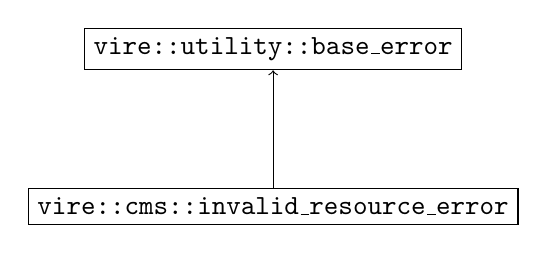
\begin{tikzpicture}
  \node (base)  at (0,2)  [draw] {\texttt{vire::utility::base\_error}};
  \node (ire)  at (0,0) [draw] {\texttt{vire::cms::invalid\_resource\_error}};
  \draw[->] (node cs:name=ire,anchor=north)
  |- (0,1) -| (node cs:name=base,anchor=south);
\end{tikzpicture}
\end{center}

\begin{figure}[h]
\vskip 10pt
\small
\begin{Verbatim}[frame=single,xleftmargin=0.cm,label=\fbox{C++}]
struct vire::cms::invalid_resource_error : public vire::utility::base_error
{
  // Attributes:
  std::string invalid_resource_path; // Invalid resource path
  std::string invalid_resource_id;   // Invalid resource internal ID (Vire server only)
};
\end{Verbatim}
\normalsize
\caption{The structure  of a invalid resource error object (C++).}
\label{fig-app-payload-invalid_resource_error}
\end{figure}

\begin{figure}[h]
\vskip 10pt
\small
\begin{Verbatim}[frame=single,xleftmargin=0.cm,label=\fbox{JSON++}]
{
  "code" : "3",
  "message_format" : "Resource path 'Atlas://Calorimeter/HV/Crate1/stop' is invalid",
  "invalid_resource_path" : "Atlas://Calorimeter/HV/Crate1/stop"
}
\end{Verbatim}
\normalsize
\caption{JSON formatted invalid resource error object.}
\label{fig-app-payload-invalid_resource_error-json}
\end{figure}


\item
Class     \texttt{vire::cms::resource\_status\_record}    (figure
\ref{fig-app-payload-resource_status_record}).

\end{itemize}

\begin{figure}[h]
\vskip 10pt
\small
\begin{Verbatim}[frame=single,xleftmargin=0.cm,label=\fbox{C++}]
struct vire::cms::resource_status_record
{
  // Attributes:
  std::string path;      // Path of the resource
  std::string timestamp; // Timestamp of the last modification
  uint16_t    flags;     // Status bits (Missing/Disabled/Pending/Error)
};
\end{Verbatim}
\normalsize
\caption{The structure  of a resource status record object (C++).}
\label{fig-app-payload-resource_status_record}
\end{figure}


\begin{figure}[h]
\vskip 10pt
\small
\begin{Verbatim}[frame=single,xleftmargin=0.cm,label=\fbox{JSON}]
{
  "path" : "SuperNEMO://Demonstrator/CMS/Coil/Control/Current/__dp_read__",
  "timestamp" : "20160612T212432.324517",
  "flags" : 2
}
\end{Verbatim}
\normalsize
\caption{JSON formatted resource status record object.}
\label{fig-app-payload-resource_status_record-json}
\end{figure}

\vfill
\pagebreak
\clearpage

\subsection{Connection of the Vire server to the CMS server}


\begin{itemize}

\item   The   \texttt{vire::cmslapp::connection\_request}   class
  (version \texttt{1.0})  represents a connection request  sent by the
  Vire server to the  CMS server through the \textcolor{blue}{service}
  channel.

\begin{center}
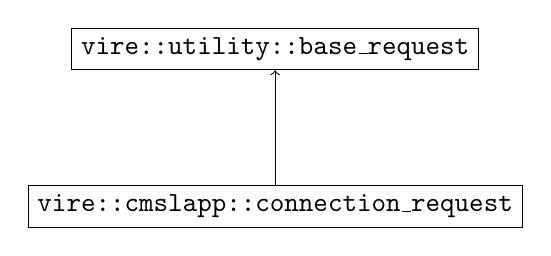
\begin{tikzpicture}
  \node (base)  at (0,2)  [draw] {\texttt{vire::utility::base\_request}};
  \node (cr)  at (0,0) [draw] {\texttt{vire::cmslapp::connection\_request}};
  \draw[->] (node cs:name=cr,anchor=north)
  |- (0,1) -| (node cs:name=base,anchor=south);
\end{tikzpicture}
\end{center}

\noindent Class registration:
\begin{itemize}
\item name: \texttt{"vire::cmslapp::connection\_request"}
\item version: "1.0"
\end{itemize}

\begin{figure}[h]
\vskip 10pt
\small
\begin{Verbatim}[frame=single,xleftmargin=0.cm,label=\fbox{C++}]
struct vire::cmslapp::connection_request : public vire::utility::base_request
{
  // Attributes:
  vire::utility::instance_identifier  setup_id; // Identifier of the experimental setup
  std::vector<std::string> requested_resources; // The list of requested resources
                                                // addressed by path
};
\end{Verbatim}
\normalsize
\caption{The structure of the connection  request object to be emitted
  by the Vire server to the CMS server (C++).}
\label{fig-app-payload-connection_request}
\end{figure}

\begin{figure}[h]
\vskip 10pt
\small
\begin{Verbatim}[frame=single,xleftmargin=0.cm,label=\fbox{JSON}]
{
  "setup_id" : {
    "name" : "snemo",
    "version" : "1.0.2"
  },
  "requested_resources" : [
    "SuperNEMO://Demonstrator/CMS/Coil/PS/Control/Current/__dp_read__",
    "SuperNEMO://Demonstrator/CMS/Coil/PS/Control/Current/__dp_write__",
    ...
    "SuperNEMO://Demonstrator/CMS/Acquisition/start",
    "SuperNEMO://Demonstrator/CMS/Acquisition/stop"
  ]
}
\end{Verbatim}
\normalsize
\caption{A JSON formatted  connection request object sent  by the Vire
  server to the CMS server (C++).}
\label{fig-app-payload-connection_request-json}
\end{figure}


\item  The  \texttt{vire::cmslapp::connection\_success\_response}
  class represents  the response sent back  to the Vire server  by the
  CMS server through the  \textcolor{blue}{service} channel in case of
  success.

\begin{center}
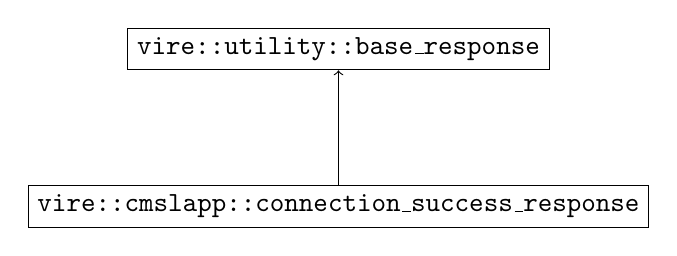
\begin{tikzpicture}
  \node (base)  at (0,2)  [draw] {\texttt{vire::utility::base\_response}};
  \node (csr)  at (0,0) [draw] {\texttt{vire::cmslapp::connection\_success\_response}};
  \draw[->] (node cs:name=csr,anchor=north)
  |- (0,1) -| (node cs:name=base,anchor=south);
\end{tikzpicture}
\end{center}

\noindent Class registration:
\begin{itemize}
\item name: \texttt{"vire::cmslapp::connection\_success\_response"}
\item version: "1.0"
\end{itemize}

\begin{figure}[h]
\vskip 10pt
\small
\begin{Verbatim}[frame=single,xleftmargin=0.cm,label=\fbox{C++}]
struct connection_success_response
  : public vire::utility::base_response
{
  typedef vire::resource::resource_status_record resource_status_record; // Type alias

  // Attributes:
  std::vector<resource_status_record> resources_snapshot; // Requested resources snapshot
};
\end{Verbatim}
\normalsize
\caption{The structure  of the connection success  response emitted by
  the CMS server to the Vire server (C++).}
\label{fig-app-payload-connection_success_response}
\end{figure}



\begin{figure}[h]
\vskip 10pt
\small
\begin{Verbatim}[frame=single,xleftmargin=0.cm,label=\fbox{\texttt{JSON}}]
{
  "resources_snapshot"  : [
    {
      "path" : "SuperNEMO://Demonstrator/CMS/Coil/PS/Control/Current/__dp_read__",
      "timestamp" : "20160612T212432.324517",
      "flags" : "0000"
    },
    {
      "path" : "SuperNEMO://Demonstrator/CMS/Coil/PS/Control/Current/__dp_write__",
      "timestamp" : "20160612T212432.328732",
      "flags" : "0000"
    },
    ...
    {
      "path" : "SuperNEMO://Demonstrator/CMS/Acquisition/start",
      "timestamp" : "20160612T212432.371671",
      "flags" : "0000"
    },
    {
      "path" : "SuperNEMO://Demonstrator/CMS/Acquisition/stop",
      "timestamp" : "20160612T212432.373624",
      "flags" : "0100"
    }
  ]
}
\end{Verbatim}
\normalsize
\caption[JSON formatted  connection success response]  {JSON formatted
  connection        success        response       object        (class
  \texttt{vire::cmslapp::connection\_success\_response}.}
\label{fig-app-payload-connection_success_response-json}
\end{figure}


\item
The  \texttt{vire::cmslapp::connection\_failure\_response}  class
represents the response sent back to the Vire server by the CMS server
through the \textcolor{blue}{service} channel in case of failure.

\begin{center}
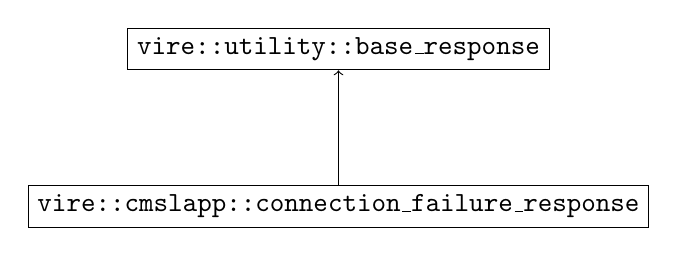
\begin{tikzpicture}
  \node (base)  at (0,2)  [draw] {\texttt{vire::utility::base\_response}};
  \node (cfr)  at (0,0) [draw] {\texttt{vire::cmslapp::connection\_failure\_response}};
  \draw[->] (node cs:name=cfr,anchor=north)
  |- (0,1) -| (node cs:name=base,anchor=south);
\end{tikzpicture}
\end{center}

\begin{figure}[h]
\vskip 10pt
\small
\begin{Verbatim}[frame=single,xleftmargin=0.cm,label=\fbox{C++}]
struct connection_failure_response
  : public vire::utility::base_response
{
  // Nested type alias:
  typedef vire::utility::model_identifier error_identifier;

  // Nested error type aliases:
  typedef vire::utility::invalid_context_error invalid_context_error;
  typedef vire::utility::invalid_setup_id_error invalid_setup_id_error;

  // Nested error type:
  struct unknown_resources_error : public vire::utility::base_error {
    std::vector<std::string> unknown_paths; // List of unknown resources' paths
  };

  // Attributes:
  error_identifier error_id; // Error type identifier
  XXX_error        error;    // Embedded error record of one of the nested error type above
};
\end{Verbatim}
\normalsize
\caption{The structure  of the  connection failure response emitted
  by the CMS server to the Vire server (C++).}
\label{fig-app-payload-connection_failure_response}
\end{figure}


\end{itemize}

% \texttt{vire::cmsserver::disconnection\_request} (version \texttt{1.0})

\vfill
\pagebreak
\clearpage


\subsection{Disconnection of the Vire server from the CMS server}

\begin{itemize}

\item  The  \texttt{vire::cmslapp::disconnection\_request}  class
  represents a  disconnection request sent  by the Vire server  to the
  CMS server through the \textcolor{blue}{service} channel.

\begin{center}
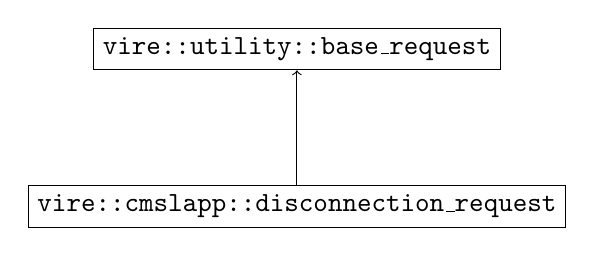
\begin{tikzpicture}
  \node (base)  at (0,2)  [draw] {\texttt{vire::utility::base\_request}};
  \node (cr)  at (0,0) [draw] {\texttt{vire::cmslapp::disconnection\_request}};
  \draw[->] (node cs:name=cr,anchor=north)
  |- (0,1) -| (node cs:name=base,anchor=south);
\end{tikzpicture}
\end{center}

\noindent Class registration:
\begin{itemize}
\item name: \texttt{"vire::cmslapp::disconnection\_request"}
\item version: "1.0"
\end{itemize}

\begin{figure}[h]
\vskip 10pt
\small
\begin{Verbatim}[frame=single,xleftmargin=0.cm,label=\fbox{C++}]
struct disconnection_request : public vire::utility::base_request {
};
\end{Verbatim}
\normalsize
\caption{The structure of the disconnection  request object to be emitted
  by the Vire server to the CMS server (C++).}
\label{fig-app-payload-disconnection_request}
\end{figure}

%% \begin{figure}[h]
%% \vskip 10pt
%% \small
%% \begin{Verbatim}[frame=single,xleftmargin=0.cm,label=\fbox{C++}]
%% {
%% }
%% \end{Verbatim}
%% \normalsize
%% \caption{A JSON formatted  connection request object sent  by the Vire
%%   server to the CMS server (C++).}
%% \label{fig-app-payload-connection_request-json}
%% \end{figure}


\item  The  \texttt{vire::cmslapp::disconnection\_success\_response}
  class represents  the response sent back  to the Vire server  by the
  CMS server through the  \textcolor{blue}{service} channel in case of
  success.

\begin{center}
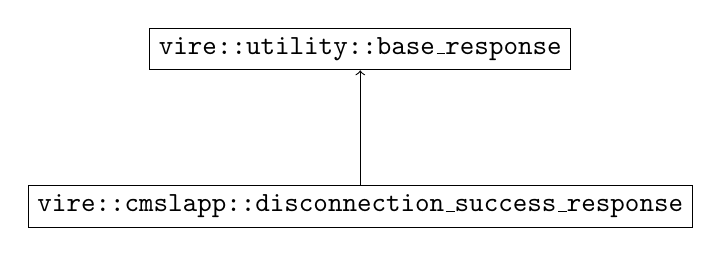
\begin{tikzpicture}
  \node (base)  at (0,2)  [draw] {\texttt{vire::utility::base\_response}};
  \node (csr)  at (0,0) [draw] {\texttt{vire::cmslapp::disconnection\_success\_response}};
  \draw[->] (node cs:name=csr,anchor=north)
  |- (0,1) -| (node cs:name=base,anchor=south);
\end{tikzpicture}
\end{center}


\noindent Class registration:
\begin{itemize}
\item name: \texttt{"vire::cmslapp::disconnection\_success\_response"}
\item version: "1.0"
\end{itemize}

\begin{figure}[h]
\vskip 10pt
\small
\begin{Verbatim}[frame=single,xleftmargin=0.cm,label=\fbox{C++}]
struct disconnection_success_response
  : public vire::utility::base_response
{
};
\end{Verbatim}
\normalsize
\caption{The structure  of the disconnection success  response emitted by
  the CMS server to the Vire server (C++).}
\label{fig-app-payload-disconnection_success_response}
\end{figure}


\end{itemize}


\vfill
\pagebreak
\clearpage

\subsection{Resource related payload objects}

\subsubsection{Resource Pub/Sub service}

\begin{itemize}

\item  The \texttt{vire::resource::resource\_pubsub\_request} object is responsible of
  demanding the activation/deactivation of the Pub/Sub service associated to a given
  resource (fig. \ref{fig-app-payload-resource_pubsub_request}).

\begin{figure}[h]
\vskip 10pt
\small
\begin{Verbatim}[frame=single,xleftmargin=0.cm,label=\fbox{C++}]
struct resource_pubsub_request
  : public vire::utility::base_request
{
  // Attributes:
  std::string path;      // The resource path.
  bool        subscribe; // Pub/Sub service (un)subscribe flag.
};
\end{Verbatim}
\normalsize
\caption{The structure of the \texttt{vire::resource::resource\_pubsub\_request}
  class (C++).}
\label{fig-app-payload-resource_pubsub_request}
\end{figure}

\item The \texttt{vire::resource::resource\_pubsub\_success\_response}
  object encapsulate a  successfull response of the CMS  server to the
  Vire  server  concerning   the  subscription/unsubscription  of  the
  Pub/Sub     service    associated     to     a    given     resource
  (fig. \ref{fig-app-payload-resource_pubsub_success_response}).

\begin{figure}[h]
\vskip 10pt
\small
\begin{Verbatim}[frame=single,xleftmargin=0.cm,label=\fbox{C++}]
struct resource_pubsub_success_response
  : public vire::utility::base_response
{
  // Pub/Sub mechanism type alias:
  typedef vire::resource::amqp_mechanism_address amqp_mechanism_address;

  // Type alias:
  typedef vire::utility::model_identifier pubsub_mechanism_identifier;
  typedef boost::variant<
      amqp_mechanism_address
      > pubsub_address_type;

  // Attributes:
  std::string                 path;               // The resource path.
  bool                        subscribe;          // The effective (un)subscribe flag.
  pubsub_mechanism_identifier pubsub_mechanism_id; // The mechanism for accessing Pub/Sub service
  pubsub_address_type         pubsub_address;      // If activation is set, this describes the
                                                   // access to the Pub/Sub service.
};
\end{Verbatim}
\normalsize
\caption{The structure of the \texttt{vire::resource::resource\_pubsub\_success\_response}
  class (C++).}
\label{fig-app-payload-resource_pubsub_success_response}
\end{figure}

\small
\begin{Verbatim}[frame=single,xleftmargin=0.cm,label=\fbox{JSON++}]
{
  "path" : "SuperNEMO://Demonstrator/CMS/Coil/PS/Monitoring/__dp_read__",
  "subscribe" : "true",
  "pubsub_mechanism_id" : "vire::amqp",
  "pubsub_address" : {
     "server" : "snemo.amqp",
     "port" : 1234,
     "channel" : "snemo.amqp.cms.pubsub.WAqq7ERzs1",
     "binding" : "SuperNEMO://Demonstrator/CMS/Coil/PS/Monitoring/__dp_read__",
     "key" : "coil.monitoring.pubsub"
  }
}
\end{Verbatim}
\normalsize

\item    The   \texttt{vire::resource::amqp\_mechanism\_address}    object
  describes   the  access   to   Pub/Sub   service  through   RabbitMQ
  (fig. \ref{fig-app-payload-amqp_pubsub_access_type}).

\begin{figure}[h]
\vskip 10pt
\small
\begin{Verbatim}[frame=single,xleftmargin=0.cm,label=\fbox{C++}]
struct amqp_mechanism_address
{
  // Attributes:
  std::string server;  // The AMQP server
  int         port;    // The AMQP server port
  std::string channel; // The RabbitMQ Pub/Sub channel.
  std::string binding; // The binding dedicated to this Pub/Sub service.
  std::string key;     // The Pub/Sub specific key/topic.
};
\end{Verbatim}
\normalsize
\caption{The structure of the \texttt{vire::resource::amqp\_pubsub\_access\_type}
  class (C++).}
\label{fig-app-payload-amqp_pubsub_access_type}
\end{figure}


\item The \texttt{vire::resource::resource\_pubsub\_failure\_response}
  object describes a failure response  concerning a request on Pub/Sub
  service       associated       to       a       given       resource
  (fig. \ref{fig-app-payload-resource_pubsub_failure_response}).


\begin{figure}[h]
\vskip 10pt
\small
\begin{Verbatim}[frame=single,xleftmargin=0.cm,label=\fbox{C++}]
struct resource_pubsub_failure_response
  : public vire::utility::base_response
{
  // Nested type alias:
  typedef vire::utility::model_identifier error_type_identifier;

  // Nested error type aliases:
  typedef vire::utility::invalid_context_error  invalid_context_error;
  typedef vire::utility::invalid_resource_error invalid_resource_error;

  // Nested error type:
  struct no_pubsub_resource_error : public vire::utility::base_error {
    std::string path; // The path of the resource without Pub/Sub service support
  };

  typedef boost::variant<
     invalid_context_error,
     invalid_resource_error,
     no_pubsub_resource_error
     > error_type;

  // Attributes:
  error_type_identifier error_type_id; // Error type identifier.
  error_type            error;        // Embedded error record of one of
                                      // the nested error types above.
};
\end{Verbatim}
\normalsize
\caption{The structure of the \texttt{vire::resource::resource\_pubsub\_failure\_response}
  class (C++).}
\label{fig-app-payload-resource_pubsub_failure_response}
\end{figure}

\end{itemize}

\vfill
\pagebreak
\clearpage

\subsubsection{Fetching resource status}

\begin{center}
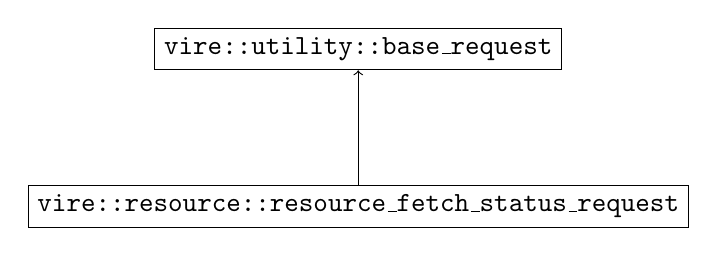
\begin{tikzpicture}
  \node (payload)  at (0,2) [draw] {\texttt{vire::utility::base\_request}};
  \node (request)  at (0,0) [draw] {\texttt{vire::resource::resource\_fetch\_status\_request}};
  \draw[->] (node cs:name=request,anchor=north)
  |- (0,1) -| (node cs:name=payload,anchor=south);
\end{tikzpicture}
\end{center}

\begin{itemize}

\item The \texttt{vire::resource::resource\_fetch\_status\_request} object
  demands to the CMS server an updated status record associated to a given resource
(fig. \ref{fig-app-payload-resource_fetch_status_request}).

\begin{figure}[h]
\vskip 10pt
\small
\begin{Verbatim}[frame=single,xleftmargin=0.cm,label=\fbox{C++}]
struct resource_fetch_status_request
  : public vire::utility::base_request
{
  // Attributes:
  std::string path; // Resource path.
};
\end{Verbatim}
\normalsize
\caption{The structure of a \texttt{vire::utility::resource\_fetch\_status\_request} object
  (C++).}
\label{fig-app-payload-resource_fetch_status_request}
\end{figure}

\item The \texttt{vire::resource::resource\_fetch\_status\_success\_response} object
  transmits the updated/current status record  associated to a given resource
(fig. \ref{fig-app-payload-resource_fetch_status_success_response}).

\begin{figure}[h]
\vskip 10pt
\small
\begin{Verbatim}[frame=single,xleftmargin=0.cm,label=\fbox{C++}]
struct resource_fetch_status_success_response
  : public vire::utility::base_response
{
  // Nested type alias:
  typedef vire::resource::resource_status_record resource_status_record;

  // Attributes:
  resource_status_record status; // The resource status record.
};
\end{Verbatim}
\normalsize
\caption{The structure of a \texttt{vire::utility::resource\_fetch\_status\_success\_response} object
  (C++).}
\label{fig-app-payload-resource_fetch_status_success_response}
\end{figure}



\item The \texttt{vire::resource::resource\_fetch\_status\_failure\_response} object
  describes a failure detected by the CMS server in response to a resource fetch status request.

\begin{figure}[h]
\vskip 10pt
\small
\begin{Verbatim}[frame=single,xleftmargin=0.cm,label=\fbox{C++}]
struct resource_fetch_status_failure_response
  : public vire::utility::base_response
{
  // Nested type alias:
  typedef vire::utility::model_identifier error_identifier;

  // Nested error type aliases:
  typedef vire::utility::invalid_context_error   invalid_context_error;
  typedef vire::resource::invalid_resource_error invalid_resource_error;

  // Attributes:
  error_identifier error_id; // Error type identifier
  XXX_error        error;    // Embedded error record of one of the nested error type above
};
\end{Verbatim}
\normalsize
\caption{The structure of a \texttt{vire::utility::resource\_fetch\_status\_failure\_response} object
  (C++).}
\label{fig-app-payload-resource_fetch_status_failure_response}
\end{figure}


\end{itemize}


\vfill
\pagebreak
\clearpage

\subsubsection{Synchronous/blocking resource execution}

\begin{center}
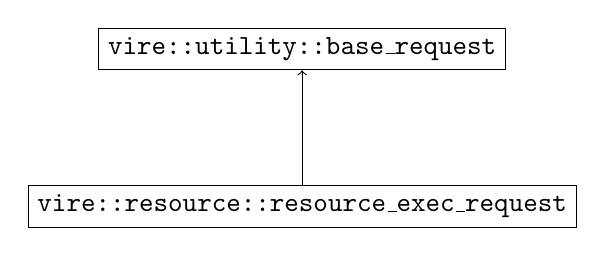
\begin{tikzpicture}
  \node (payload)  at (0,2)   [draw] {\texttt{vire::utility::base\_request}};
  \node (request)  at (0,0)  [draw] {\texttt{vire::resource::resource\_exec\_request}};
  \draw[->] (node cs:name=request,anchor=north)
  |- (0,1) -| (node cs:name=payload,anchor=south);
\end{tikzpicture}
\end{center}

\begin{itemize}

\item The \texttt{vire::resource::resource\_exec\_request} object represent a resource execution request
in blocking (synchronous) mode.


\begin{figure}[h]
\vskip 10pt
\small
\begin{Verbatim}[frame=single,xleftmargin=0.cm,label=\fbox{C++}]
struct resource_exec_request
  : public vire::utility::base_request
{
  // Type alias:
  typedef vire::resource::method_argument method_argument;

  // Attributes:
  std::string                  path;            // Resource path.
  std::vector<method_argument> input_arguments; // Embedded error record of one of
                                                // the nested error type above.
};
\end{Verbatim}
\normalsize
\caption{The structure of a \texttt{vire::utility::resource\_fetch\_status\_failure\_response} object
  (C++).}
\label{fig-app-payload-resource_fetch_status_failure_response}
\end{figure}

\item \texttt{vire::resource::resource\_exec\_success\_response}

\small
\begin{Verbatim}[frame=single,xleftmargin=0.cm,label=\fbox{C++}]
struct resource_exec_success_response
 : vire::utility::base_response
{
  // Type alias:
  typedef vire::resource::method_argument        method_argument;
  typedef vire::resource::resource_status_record resource_status_record;

  // Attributes:
  resource_status_record       status;               // Resource status
  std::string                  reception_timestamp;  // Request reception timestamp
  std::string                  completion_timestamp; // Execution completion timestamp
  std::vector<method_argument> output_arguments;     // Output arguments
};
\end{Verbatim}



\item \texttt{vire::resource::resource\_exec\_failure\_response}


\small
\begin{Verbatim}[frame=single,xleftmargin=0.cm,label=\fbox{C++}]
struct resource_exec_failure_response
 : vire::utility::base_response
{

  // Error type aliases:
  typedef vire::utility::invalid_context_error   invalid_context_error;
  typedef vire::resource::invalid_resource_error invalid_resource_error;
  typedef vire::resource::invalid_status_error   invalid_status_error;
  typedef vire::resource::resource_exec_error    resource_exec_error;

  // Type aliases:
  typedef vire::utility::model_identifier        error_type_identifier;
  typedef boost::variant<
      invalid_context_error,
      invalid_resource_error,
      invalid_status_error,
      resource_exec_error> error_type;

  // Attributes:
  error_type_identifier error_type_id; // Error type identifier
  error_type            error;        // Embedded error record

};
\end{Verbatim}

\end{itemize}


\vfill
\pagebreak
\clearpage

\subsubsection{Asynchronous/non-blocking resource execution}

\begin{center}
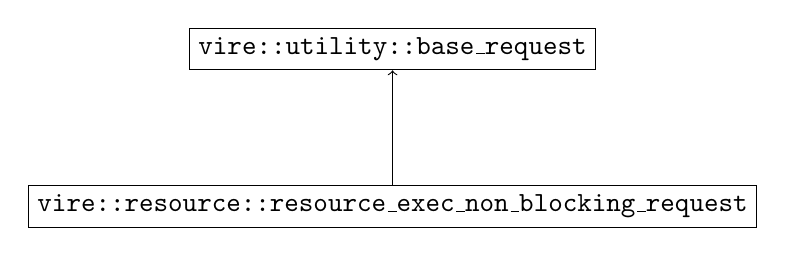
\begin{tikzpicture}
  \node (payload)  at (0,2)   [draw] {\texttt{vire::utility::base\_request}};
  \node (request_nb)  at (0,0)  [draw] {\texttt{vire::resource::resource\_exec\_non\_blocking\_request}};
  \draw[->] (node cs:name=request_nb,anchor=north)
  |- (0,1) -| (node cs:name=payload,anchor=south);
\end{tikzpicture}
\end{center}

\begin{itemize}

\item \texttt{vire::resource::resource\_exec\_non\_blocking\_request}
\small
\begin{Verbatim}[frame=single,xleftmargin=0.cm,label=\fbox{C++}]
struct resource_exec_non_blocking_request
  : public vire::utility::base_request
{
  // Type alias:
  typedef vire::resource::method_argument method_argument;

  // Attributes:
  std::string                  path;            // Resource path.
  std::vector<method_argument> input_arguments; // Embedded error record of one of
                                                // the nested error type above.

};
\end{Verbatim}

\item \texttt{vire::resource::resource\_exec\_non\_blocking\_ack\_response}


\small
\begin{Verbatim}[frame=single,xleftmargin=0.cm,label=\fbox{C++}]
struct resource_exec_non_blocking_ack_response
 : vire::utility::base_response
{
  // Type alias:
  typedef vire::resource::method_argument        method_argument;
  typedef vire::resource::resource_status_record resource_status_record;

  // Attributes:
  resource_status_record       status;
  std::string                  reception_timestamp;

};
\end{Verbatim}


\item \texttt{vire::resource::resource\_exec\_non\_blocking\_noack\_response}


\small
\begin{Verbatim}[frame=single,xleftmargin=0.cm,label=\fbox{C++}]
struct resource_exec_non_blocking_noack_response
  : vire::utility::base_response
{
  // Type alias:
  typedef vire::resource::resource_status_record resource_status_record;
  typedef vire::utility::model_identifier error_type_identifier;

  // Error type aliases:
  typedef vire::utility::invalid_context_error   invalid_context_error;
  typedef vire::resource::invalid_resource_error invalid_resource_error;
  typedef vire::resource::invalid_status_error   invalid_status_error;
  typedef vire::resource::resource_exec_error    resource_exec_error;

  // Nested error type:
  struct no_non_blocking_exec_resource_error : public vire::utility::base_error {
    std::string path; // The path of the resource without non-blocking execution support
  };

  typedef boost::variant<
     invalid_context_error,
     invalid_resource_error,
     invalid_status_error,
     no_non_blocking_exec_resource_error,
     resource_exec_error
     > error_type;

  // Attributes:
  resource_status_record status;        // Resource status.
  error_type_identifier  error_type_id; // Error type identifier.
  error_type             error;         // Embedded error record of one of
                                        // the nested error types above.

};
\end{Verbatim}
\normalsize


\item \texttt{vire::resource::resource\_exec\_non\_blocking\_success\_event}


\small
\begin{Verbatim}[frame=single,xleftmargin=0.cm,label=\fbox{C++}]
struct resource_exec_non_blocking_success\_event
  : vire::utility::base_event
{
  // Type alias:
  typedef vire::resource::method_argument        method_argument;
  typedef vire::resource::resource_status_record resource_status_record;

  // Attributes:
  resource_status_record       status;               // Resource status
  std::string                  reception_timestamp;  // Request reception timestamp
  std::string                  completion_timestamp; // Execution completion timestamp
  std::vector<method_argument> output_arguments;     // Output arguments

};
\end{Verbatim}
\normalsize

\item \texttt{vire::resource::resource\_exec\_non\_blocking\_failure\_event}


\small
\begin{Verbatim}[frame=single,xleftmargin=0.cm,label=\fbox{C++}]
struct resource_exec_non_blocking_failure\_event
  : vire::utility::base_event
{

  // Error type aliases:
  typedef vire::utility::invalid_context_error   invalid_context_error;
  typedef vire::cms::invalid_resource_error invalid_resource_error;
  typedef vire::cms::invalid_status_error   invalid_status_error;
  typedef vire::cms::resource_exec_error    resource_exec_error;

  // Type aliases:
  typedef vire::utility::model_identifier        error_type_identifier;
  typedef boost::variant<
      vire::utility::invalid_context_error,
      vire::cms::invalid_resource_error,
      vire::cms::invalid_status_error,
      vire::cms::resource_exec_error> error_type;

  // Attributes:
  error_type_identifier error_type_id; // Error type identifier
  error_type            error;        // Embedded error record

};
\end{Verbatim}
\normalsize


\end{itemize}


\vfill
\pagebreak
\clearpage

% end


\section{The RabbitMQ based RPC system}\label{app:rabbitmq_rpc}

\subsection{Introduction}


\end{document}
%%

\vfill
\pagebreak
\clearpage

% \documentclass[a4paper,11pt,twoside]{article}

%%% packages:
\usepackage[T1]{fontenc}
\usepackage{ucs}
\usepackage[utf8x]{inputenc}
%\usepackage[frenchb]{babel}
\usepackage{amsmath}
\usepackage{amssymb}
\usepackage{latexsym}
\usepackage{verbatim}
\usepackage{moreverb}
\usepackage{fancyvrb}
\usepackage{alltt}
\usepackage{eurosym}
\usepackage{hyperref}
\usepackage{colortbl}
\usepackage{graphicx}
\usepackage{pdflscape}
\usepackage{afterpage}
\usepackage{rotating}
\usepackage{tikz}
%\usepackage{tikz-qtree}

%%% Geometry (https://en.wikibooks.org/wiki/LaTeX/Page_Layout)
\usepackage{layout}
%\usepackage[a4paper,top=1in, bottom=1.25in, left=1.25in, right=1.25in, inner=4cm,outer=2cm]{geometry}
\usepackage[a4paper,inner=2cm,outer=2cm]{geometry}
%% \setlength{\hoffset}{-1inch}
%% \setlength{\voffset}{-1inch0pt}
\setlength{\textheight}{23cm}
%% \setlength{\textwidth}{18cm}

%%% macros:
\newcommand{\thepath}{.}
\newcommand{\imgpath}{\thepath/images}
\newcommand{\pdfteximgpath}{\thepath/pdftex}
\newcommand{\pdftextimgpath}{\thepath/pdftex_t}

%%%
\title{The SuperNEMO Vire-CMS/LAPP interface\\version 0.7}
\author{E.Chabanne, J.Hommet, T. Leflour, Y. Lemière,
  S.Lieunard, F.Mauger, J.-L. Panazol, J.Poincheval}
\date{\today}

%%%
\begin{document}

\thispagestyle{empty}
%\layout{}
\maketitle
\begin{abstract}
This document aims  to describe the requirements of  the Vire CMS/LAPP
interface,  i.e. the  software bridge  between the  Vire based  online
software  (Vire server  and clients,  a.k.a the  Vire system)  and the
CMS/LAPP server  that plays  the role  of the  unique gate  (subcontractor proxy) to
communicate with  the OPCUA-based MOS  servers responsible of  the low
level control and monitoring operations on some hardware devices.
\end{abstract}
\vfill
\pagebreak

\tableofcontents
\vfill
\pagebreak

\listoffigures
\vfill
\pagebreak

\listoftables
\vfill
\pagebreak
\clearpage

\documentclass[a4paper,11pt,twoside]{article}

%%% packages:
\usepackage[T1]{fontenc}
\usepackage{ucs}
\usepackage[utf8x]{inputenc}
%\usepackage[frenchb]{babel}
\usepackage{amsmath}
\usepackage{amssymb}
\usepackage{latexsym}
\usepackage{verbatim}
\usepackage{moreverb}
\usepackage{fancyvrb}
\usepackage{alltt}
\usepackage{eurosym}
\usepackage{hyperref}
\usepackage{colortbl}
\usepackage{graphicx}
\usepackage{pdflscape}
\usepackage{afterpage}
\usepackage{rotating}
\usepackage{tikz}
%\usepackage{tikz-qtree}

%%% Geometry (https://en.wikibooks.org/wiki/LaTeX/Page_Layout)
\usepackage{layout}
%\usepackage[a4paper,top=1in, bottom=1.25in, left=1.25in, right=1.25in, inner=4cm,outer=2cm]{geometry}
\usepackage[a4paper,inner=2cm,outer=2cm]{geometry}
%% \setlength{\hoffset}{-1inch}
%% \setlength{\voffset}{-1inch0pt}
\setlength{\textheight}{23cm}
%% \setlength{\textwidth}{18cm}

%%% macros:
\newcommand{\thepath}{.}
\newcommand{\imgpath}{\thepath/images}
\newcommand{\pdfteximgpath}{\thepath/pdftex}
\newcommand{\pdftextimgpath}{\thepath/pdftex_t}

%%%
\title{The SuperNEMO Vire-CMS/LAPP interface\\version 0.7}
\author{E.Chabanne, J.Hommet, T. Leflour, Y. Lemière,
  S.Lieunard, F.Mauger, J.-L. Panazol, J.Poincheval}
\date{\today}

%%%
\begin{document}

\thispagestyle{empty}
%\layout{}
\maketitle
\begin{abstract}
This document aims  to describe the requirements of  the Vire CMS/LAPP
interface,  i.e. the  software bridge  between the  Vire based  online
software  (Vire server  and clients,  a.k.a the  Vire system)  and the
CMS/LAPP server  that plays  the role  of the  unique gate  (subcontractor proxy) to
communicate with  the OPCUA-based MOS  servers responsible of  the low
level control and monitoring operations on some hardware devices.
\end{abstract}
\vfill
\pagebreak

\tableofcontents
\vfill
\pagebreak

\listoffigures
\vfill
\pagebreak

\listoftables
\vfill
\pagebreak
\clearpage

\input{cms_server/main.tex}
\vfill
\pagebreak
\clearpage

\input{vire_resources/main.tex}
\vfill
\pagebreak
\clearpage

% \input{cmslapp_vireclients/main.tex}
\section{Interaction of the CMS/LAPP server with Vire clients}

TODO
\vfill
\pagebreak
\clearpage

%%%%%%%%%
\appendix

\input{appendix/app_filesystem.tex}
\input{appendix/app_new_device.tex}
\input{appendix/app_vire_messages.tex}
%\input{appendix/app_json_fmt.tex}
\input{appendix/app_protobuf_format.tex}
\input{appendix/app_payload_objects.tex}
\input{appendix/app_rabbitmq_rpc.tex}

\end{document}
%%

\vfill
\pagebreak
\clearpage

\documentclass[a4paper,11pt,twoside]{article}

%%% packages:
\usepackage[T1]{fontenc}
\usepackage{ucs}
\usepackage[utf8x]{inputenc}
%\usepackage[frenchb]{babel}
\usepackage{amsmath}
\usepackage{amssymb}
\usepackage{latexsym}
\usepackage{verbatim}
\usepackage{moreverb}
\usepackage{fancyvrb}
\usepackage{alltt}
\usepackage{eurosym}
\usepackage{hyperref}
\usepackage{colortbl}
\usepackage{graphicx}
\usepackage{pdflscape}
\usepackage{afterpage}
\usepackage{rotating}
\usepackage{tikz}
%\usepackage{tikz-qtree}

%%% Geometry (https://en.wikibooks.org/wiki/LaTeX/Page_Layout)
\usepackage{layout}
%\usepackage[a4paper,top=1in, bottom=1.25in, left=1.25in, right=1.25in, inner=4cm,outer=2cm]{geometry}
\usepackage[a4paper,inner=2cm,outer=2cm]{geometry}
%% \setlength{\hoffset}{-1inch}
%% \setlength{\voffset}{-1inch0pt}
\setlength{\textheight}{23cm}
%% \setlength{\textwidth}{18cm}

%%% macros:
\newcommand{\thepath}{.}
\newcommand{\imgpath}{\thepath/images}
\newcommand{\pdfteximgpath}{\thepath/pdftex}
\newcommand{\pdftextimgpath}{\thepath/pdftex_t}

%%%
\title{The SuperNEMO Vire-CMS/LAPP interface\\version 0.7}
\author{E.Chabanne, J.Hommet, T. Leflour, Y. Lemière,
  S.Lieunard, F.Mauger, J.-L. Panazol, J.Poincheval}
\date{\today}

%%%
\begin{document}

\thispagestyle{empty}
%\layout{}
\maketitle
\begin{abstract}
This document aims  to describe the requirements of  the Vire CMS/LAPP
interface,  i.e. the  software bridge  between the  Vire based  online
software  (Vire server  and clients,  a.k.a the  Vire system)  and the
CMS/LAPP server  that plays  the role  of the  unique gate  (subcontractor proxy) to
communicate with  the OPCUA-based MOS  servers responsible of  the low
level control and monitoring operations on some hardware devices.
\end{abstract}
\vfill
\pagebreak

\tableofcontents
\vfill
\pagebreak

\listoffigures
\vfill
\pagebreak

\listoftables
\vfill
\pagebreak
\clearpage

\input{cms_server/main.tex}
\vfill
\pagebreak
\clearpage

\input{vire_resources/main.tex}
\vfill
\pagebreak
\clearpage

% \input{cmslapp_vireclients/main.tex}
\section{Interaction of the CMS/LAPP server with Vire clients}

TODO
\vfill
\pagebreak
\clearpage

%%%%%%%%%
\appendix

\input{appendix/app_filesystem.tex}
\input{appendix/app_new_device.tex}
\input{appendix/app_vire_messages.tex}
%\input{appendix/app_json_fmt.tex}
\input{appendix/app_protobuf_format.tex}
\input{appendix/app_payload_objects.tex}
\input{appendix/app_rabbitmq_rpc.tex}

\end{document}
%%

\vfill
\pagebreak
\clearpage

% \documentclass[a4paper,11pt,twoside]{article}

%%% packages:
\usepackage[T1]{fontenc}
\usepackage{ucs}
\usepackage[utf8x]{inputenc}
%\usepackage[frenchb]{babel}
\usepackage{amsmath}
\usepackage{amssymb}
\usepackage{latexsym}
\usepackage{verbatim}
\usepackage{moreverb}
\usepackage{fancyvrb}
\usepackage{alltt}
\usepackage{eurosym}
\usepackage{hyperref}
\usepackage{colortbl}
\usepackage{graphicx}
\usepackage{pdflscape}
\usepackage{afterpage}
\usepackage{rotating}
\usepackage{tikz}
%\usepackage{tikz-qtree}

%%% Geometry (https://en.wikibooks.org/wiki/LaTeX/Page_Layout)
\usepackage{layout}
%\usepackage[a4paper,top=1in, bottom=1.25in, left=1.25in, right=1.25in, inner=4cm,outer=2cm]{geometry}
\usepackage[a4paper,inner=2cm,outer=2cm]{geometry}
%% \setlength{\hoffset}{-1inch}
%% \setlength{\voffset}{-1inch0pt}
\setlength{\textheight}{23cm}
%% \setlength{\textwidth}{18cm}

%%% macros:
\newcommand{\thepath}{.}
\newcommand{\imgpath}{\thepath/images}
\newcommand{\pdfteximgpath}{\thepath/pdftex}
\newcommand{\pdftextimgpath}{\thepath/pdftex_t}

%%%
\title{The SuperNEMO Vire-CMS/LAPP interface\\version 0.7}
\author{E.Chabanne, J.Hommet, T. Leflour, Y. Lemière,
  S.Lieunard, F.Mauger, J.-L. Panazol, J.Poincheval}
\date{\today}

%%%
\begin{document}

\thispagestyle{empty}
%\layout{}
\maketitle
\begin{abstract}
This document aims  to describe the requirements of  the Vire CMS/LAPP
interface,  i.e. the  software bridge  between the  Vire based  online
software  (Vire server  and clients,  a.k.a the  Vire system)  and the
CMS/LAPP server  that plays  the role  of the  unique gate  (subcontractor proxy) to
communicate with  the OPCUA-based MOS  servers responsible of  the low
level control and monitoring operations on some hardware devices.
\end{abstract}
\vfill
\pagebreak

\tableofcontents
\vfill
\pagebreak

\listoffigures
\vfill
\pagebreak

\listoftables
\vfill
\pagebreak
\clearpage

\input{cms_server/main.tex}
\vfill
\pagebreak
\clearpage

\input{vire_resources/main.tex}
\vfill
\pagebreak
\clearpage

% \input{cmslapp_vireclients/main.tex}
\section{Interaction of the CMS/LAPP server with Vire clients}

TODO
\vfill
\pagebreak
\clearpage

%%%%%%%%%
\appendix

\input{appendix/app_filesystem.tex}
\input{appendix/app_new_device.tex}
\input{appendix/app_vire_messages.tex}
%\input{appendix/app_json_fmt.tex}
\input{appendix/app_protobuf_format.tex}
\input{appendix/app_payload_objects.tex}
\input{appendix/app_rabbitmq_rpc.tex}

\end{document}
%%

\section{Interaction of the CMS/LAPP server with Vire clients}

TODO
\vfill
\pagebreak
\clearpage

%%%%%%%%%
\appendix


\section{Filesystem and configuration files management}\label{app:filesystem_conf}

Let's consider  a simple  situation where  one runs  the Vire  and CMS
software  tools (servers)  on a  single Linux  machine (the  CMS host)
under            the            \texttt{"nemoprod"}            generic
account\footnote{\texttt{"nemoprod"}  is  the   login  of  th  generic
  account used at the CCIN2P3  cluster to perform automated management
  operations on experimental and  Monte-Carlo data file: data transfer
  from LSM or LSC labs to CCIN2P3, calibration and reconstruction data
  processing, storage on HPPS.}.

\begin{itemize}
\item Hostname login : \verb|192.168.1.10| (private IP) %\texttt{snemocms.lsm.in2p3.fr} (public address)
\item User login : \texttt{nemoprod}
\item Main group : \texttt{supernemo}
\item Home directory : \verb|/home/nemoprod| (a.k.a. \verb|~nemoprod|)
\end{itemize}

\noindent  We  assume that  the  SuperNEMO  online software  has  been
installed   and  setup   in  the   home  directory,   for  example in
\verb|/home/nemoprod/Private/Software/| :
\vskip 20pt
\small
\begin{Verbatim}[frame=single,xleftmargin=0.cm,label=\fbox{Filesystem}]
/home/nemoprod/Private/Software
|-- Cadfael/ # base directory of the Cadfael software framework
|-- Bayeux/  # base directory of the Bayeux software framework
|-- Vire/    # base directory of the Vire software framework
|-- OPCUA/   # base directory of the OPCUA+MOS software framework
`-- Falaise/ # base directory of the Falaise software framework
\end{Verbatim}
\normalsize

\noindent  We consider  here  that the  Falaise  library package  will
contain  the mandatory  configuration files  that describe  the online
software, both for the Vire and CMS/MOS parts:
\vskip 20pt
\small
\begin{Verbatim}[frame=single,xleftmargin=0.cm,label=\fbox{Filesystem}]
/home/nemoprod/Private/Software
:
`-- Falaise/
    :
    `-- Install/
        `-- Falaise-3.0.0/
            |-- bin/
            |   :
            |   |-- flquery
            |   |-- flreconstruct
            |   `-- flsimulate
            |-- include/
            :   :
            |-- lib/
            |   `-- x86_64-linux-gnu/
            |       :
            |       |-- libFalaise.so
            |       :
            `-- share/
                `-- Falaise-3.0.0/
                    `-- resources/
                        `-- config/
                            `-- online/
                                :
                                :
\end{Verbatim}
\normalsize

\noindent Where:
\begin{itemize}
\item                                                              the
  \verb|/home/nemoprod/Private/Software/Falaise/Install/Falaise-3.0.0|
  is  the  installation  prefix  of  the  Falaise  library  (binaries,
  includes) and associated resource files.
\item      the     \verb|share/Falaise-3.0.0/resources/config/online/|
  subdirectory  is the  tree  of configuration  files  that should  be
  accessible  by  any online  software  component  (Vire server,  Vire
  clients, CMS and MOS servers).
\end{itemize}


\noindent  Let's consider  the \verb|.../config/online/|  directory as
the base directory for all online configuration files for the Vire and
CMS  servers.   All  configuration  files  should  thus  be  addressed
relatively to this place.

\noindent  We  propose to  use  one  of  the following  techniques  to
represent this base directory:

\begin{itemize}
\item         a         dedicated         environment         variable
  \verb|SNEMO_ONLINE_CONFIG_BASE_DIR| recognized by  both Vire and CMS
  servers. It could be setup within the environment with:
\vskip 20pt
\small
\begin{Verbatim}[frame=single,xleftmargin=0.cm,label=\fbox{shell}]
export FALAISE_INSTALL_DIR=\
  ${HOME}/Private/Software/Falaise/Install/Falaise-3.0.0
export SNEMO_ONLINE_CONFIG_BASE_DIR=\
  ${FALAISE_INSTALL_DIR}/share/Falaise-3.0.0/resources/config/online
\end{Verbatim}
\normalsize

\item a  path registration label as  implemented in the kernel  of the
  Bayeux library:\\
  \noindent The \verb|@snonlinecfg:| label \\
  is associated to\\
  \noindent \hskip 50pt\verb|${FALAISE_INSTALL_DIR}/share/Falaise-3.0.0/resources/config/online|

\end{itemize}

\noindent Thus a specific  configuration file \verb|dummy.conf| could be
addressed with one of the following syntaxes:

\begin{itemize}

\item[(a)]
  \verb|${SNEMO_ONLINE_CONFIG_BASE_DIR}/snemo/1.0.2/dummy.conf|       :
  supported  by  Vire  and  CMS  using  word  expansion  utility  like
  \texttt{wordexp} (for C/C++ languages),

\item[(b)]  \verb|@snonlinecfg:snemo/1.0.2/dummy.conf|  : supported  by
  Vire  only  for  now,  thanks to  the  path  registration  mechanism
  implemented in the Bayeux API,

\item[(c)] \verb|snemo/1.0.2/dummy.conf| : can be supported by Vire and
  CMS  but  is  ambiguous  because  such a relative  path  can  be  also
  interpreted as a path relatively  to the current directory (\verb|./|)
  and not to the online configuration directory.

\end{itemize}

We suggests  the use  of an  explicit environment  variable as  in (a)
because it  is simple to  implement in various languages  and software
frameworks and should not imply any ambiguous file path resolution.

\vfill
\pagebreak
\clearpage

% end


\section{Integration of a new device}\label{app:new_device}

Both Vire  and MOS systems are  designed to be expandable  in terms of
device integration.  This section  decribes the  integration of  a new
device in the \emph{Control and Monitoring System}.

\subsection{Integration of a new device in the MOS environment}

Any new device is described through  a dedicated XML model file.  This
XML  file  is  created  from  a  template  file  elaborated  from  the
\emph{interface control document} (ICD) and associated to the model of
the  device. The  format  of the  XML  file is  described  in the  MOS
(Multipurpose OPCUA Server) User Guide. % ref

Typically, a device is embedded in a OPCUA server and implemented as a
OPCUA  \emph{simple  device}.   The  OPCUA server  itself  is  located
through an unique dedicated IP address and port.

The simple device  instance, hosted in the OPCUA  server, may contains
other sub-devices and/or \emph{datapoints}.   It is thus considered as
the root  of a hierarchy  of daughter  objects at deeper  levels.  The
daughter objects (devices or datapoints) are named relatively to their
top level  parent device. Figure  \ref{fig:an:mos_dev_1} shows an
example of a device embedded in a MOS server.

\begin{figure}[h]
\begin{center}
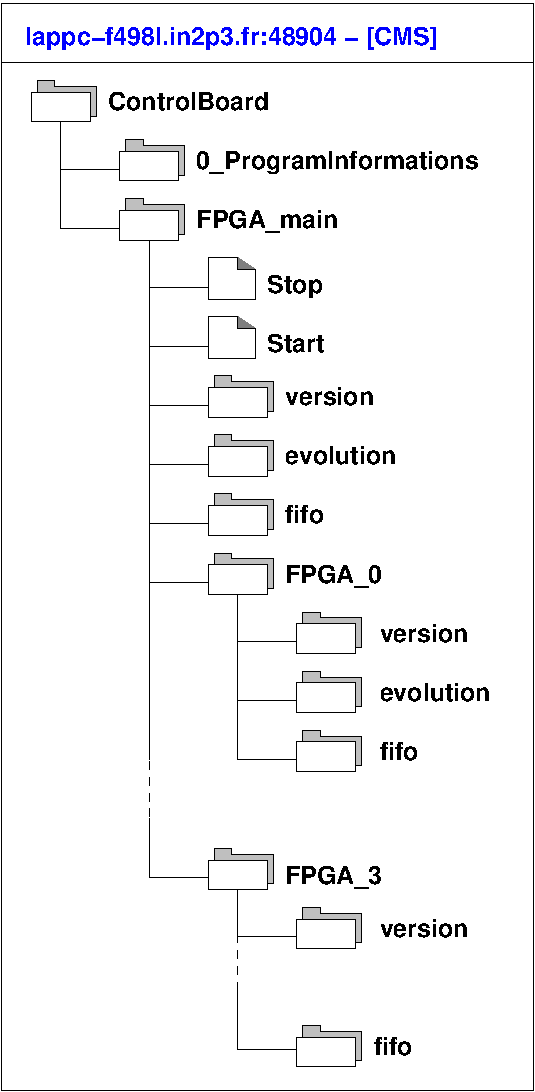
\includegraphics[width=5cm]{appendix/images/MOS_device_example_1.pdf}
\end{center}
\caption{Example of a  device managed through a MOS  server.  The root
  device is named \texttt{ControlBoard}.  First level daughter devices
  are  \texttt{0\_ProgramInformations} and  \texttt{FPGA\_main}.  Here
  the          MOS/OPCUA          server          is          labelled
  \texttt{CMS}.}\label{fig:an:mos_dev_1}
\end{figure}

% TODO


\subsection{Integration of a new device in the Vire environment}

The Vire  API also implements a  mechanism to describe a  hierarchy of
devices.  This  mechanism is independant  of the  one used in  the MOS
system but can  be easily made compatible with it.   This means that a
MOS  hierarchy  of devices  can  be  represented  in Vire.   The  Vire
hierarchy of  devices can  be considered as  some kind  of filesystem,
each device  being a folder with  its unique path, as  shown on figure
\ref{fig:an:mos_dev_2}.   The \emph{methods}  associated to  a devices
(or a datapoint) can be considered as plain executable files stored in
the  device's folder  : they  constitute the  set of  \emph{resources}
associated to the device.


\begin{figure}[h]
\begin{center}
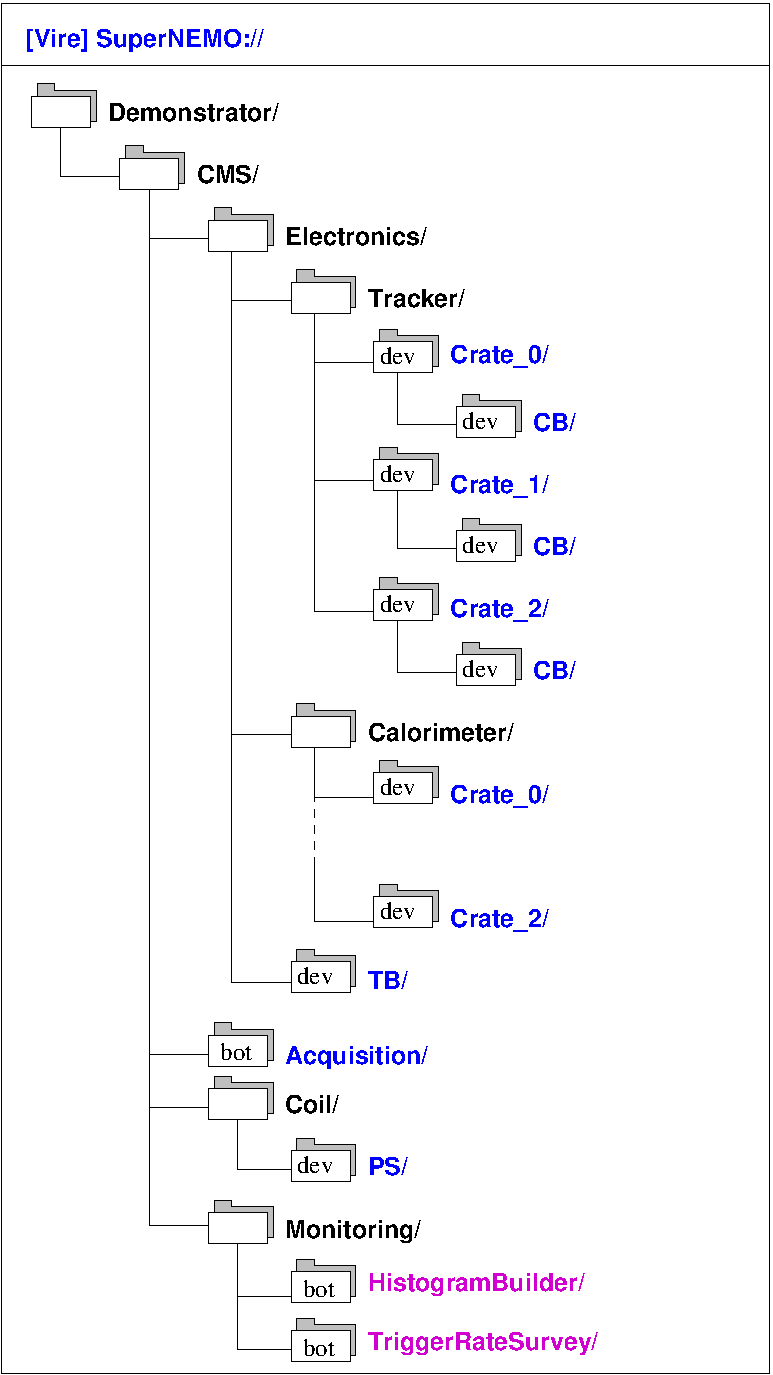
\includegraphics[width=5cm]{appendix/images/MOS_device_example_2.pdf}
\end{center}
\caption{Example of a hierarchy of  devices described by the Vire API.
  The root device is named  \texttt{SuperNEMO:}.  The top level (root)
  device  is  named  \texttt{Demonstrator}.  The  devices  colored  in
  \textcolor{blue}{blue}  are managed  through MOS/OPCUA.  The devices
  colored in \textcolor{magenta}{magenta} are directly embedded in the
  Vire server.  Devices with the \texttt{dev} tag are typical hardware
  device.  Devices  with the  \texttt{bot}  tag  are typical  software
  devices.   The  devices  colored in  \textbf{black}  are  structural
  pseudo-devices used to organize and  present a comprehensive view of
  the hierarchy. }\label{fig:an:mos_dev_2}
\end{figure}

The organisation of this hierarchy of devices is arbitrary and defined
by the designer of the  \emph{Control and Monitoring System}.  What is
important  to  understand  is  that  some  of  these  devices  can  be
associated  to  \emph{hardware  devices}  (a  power  supply  crate,  a
temperature probe\dots) and others  can be \emph{pseudo-devices}, i.e.
pure   software  object   (a   monitoring  robot,   a  file   transfer
daemon\dots).

In the context of the coupling of  the Vire server and the CMS server,
we are  in the event that  some devices are managed  by some MOS/OPCUA
servers and others are managed  in the Vire server itself.  Typically,
\emph{hardware devices}  are systematically managed through  the OPCUA
technology.  Vire has a mechanism to integrate such devices in its own
hierarchy.  This mechanism can  be considered like the \emph{mounting}
of   a   remote   filesystem   from  a   local   filesystem.    Figure
\ref{fig:an:mos_dev_0} illustrates  the case of many  hardware devices
-- managed by MOS -- that are integrated in the Vire system.  From the
Vire point of  view, the user does not see  the implementation details
for such  devices. He  does not  know the identity  of the  MOS server
hosting the device. He does not even know if the device is hosted by a
MOS server.  Devices are simply visible through the standard hierarchy
published by Vire with its  own device naming scheme, regardless their
true location.



\begin{figure}[h]
\begin{center}
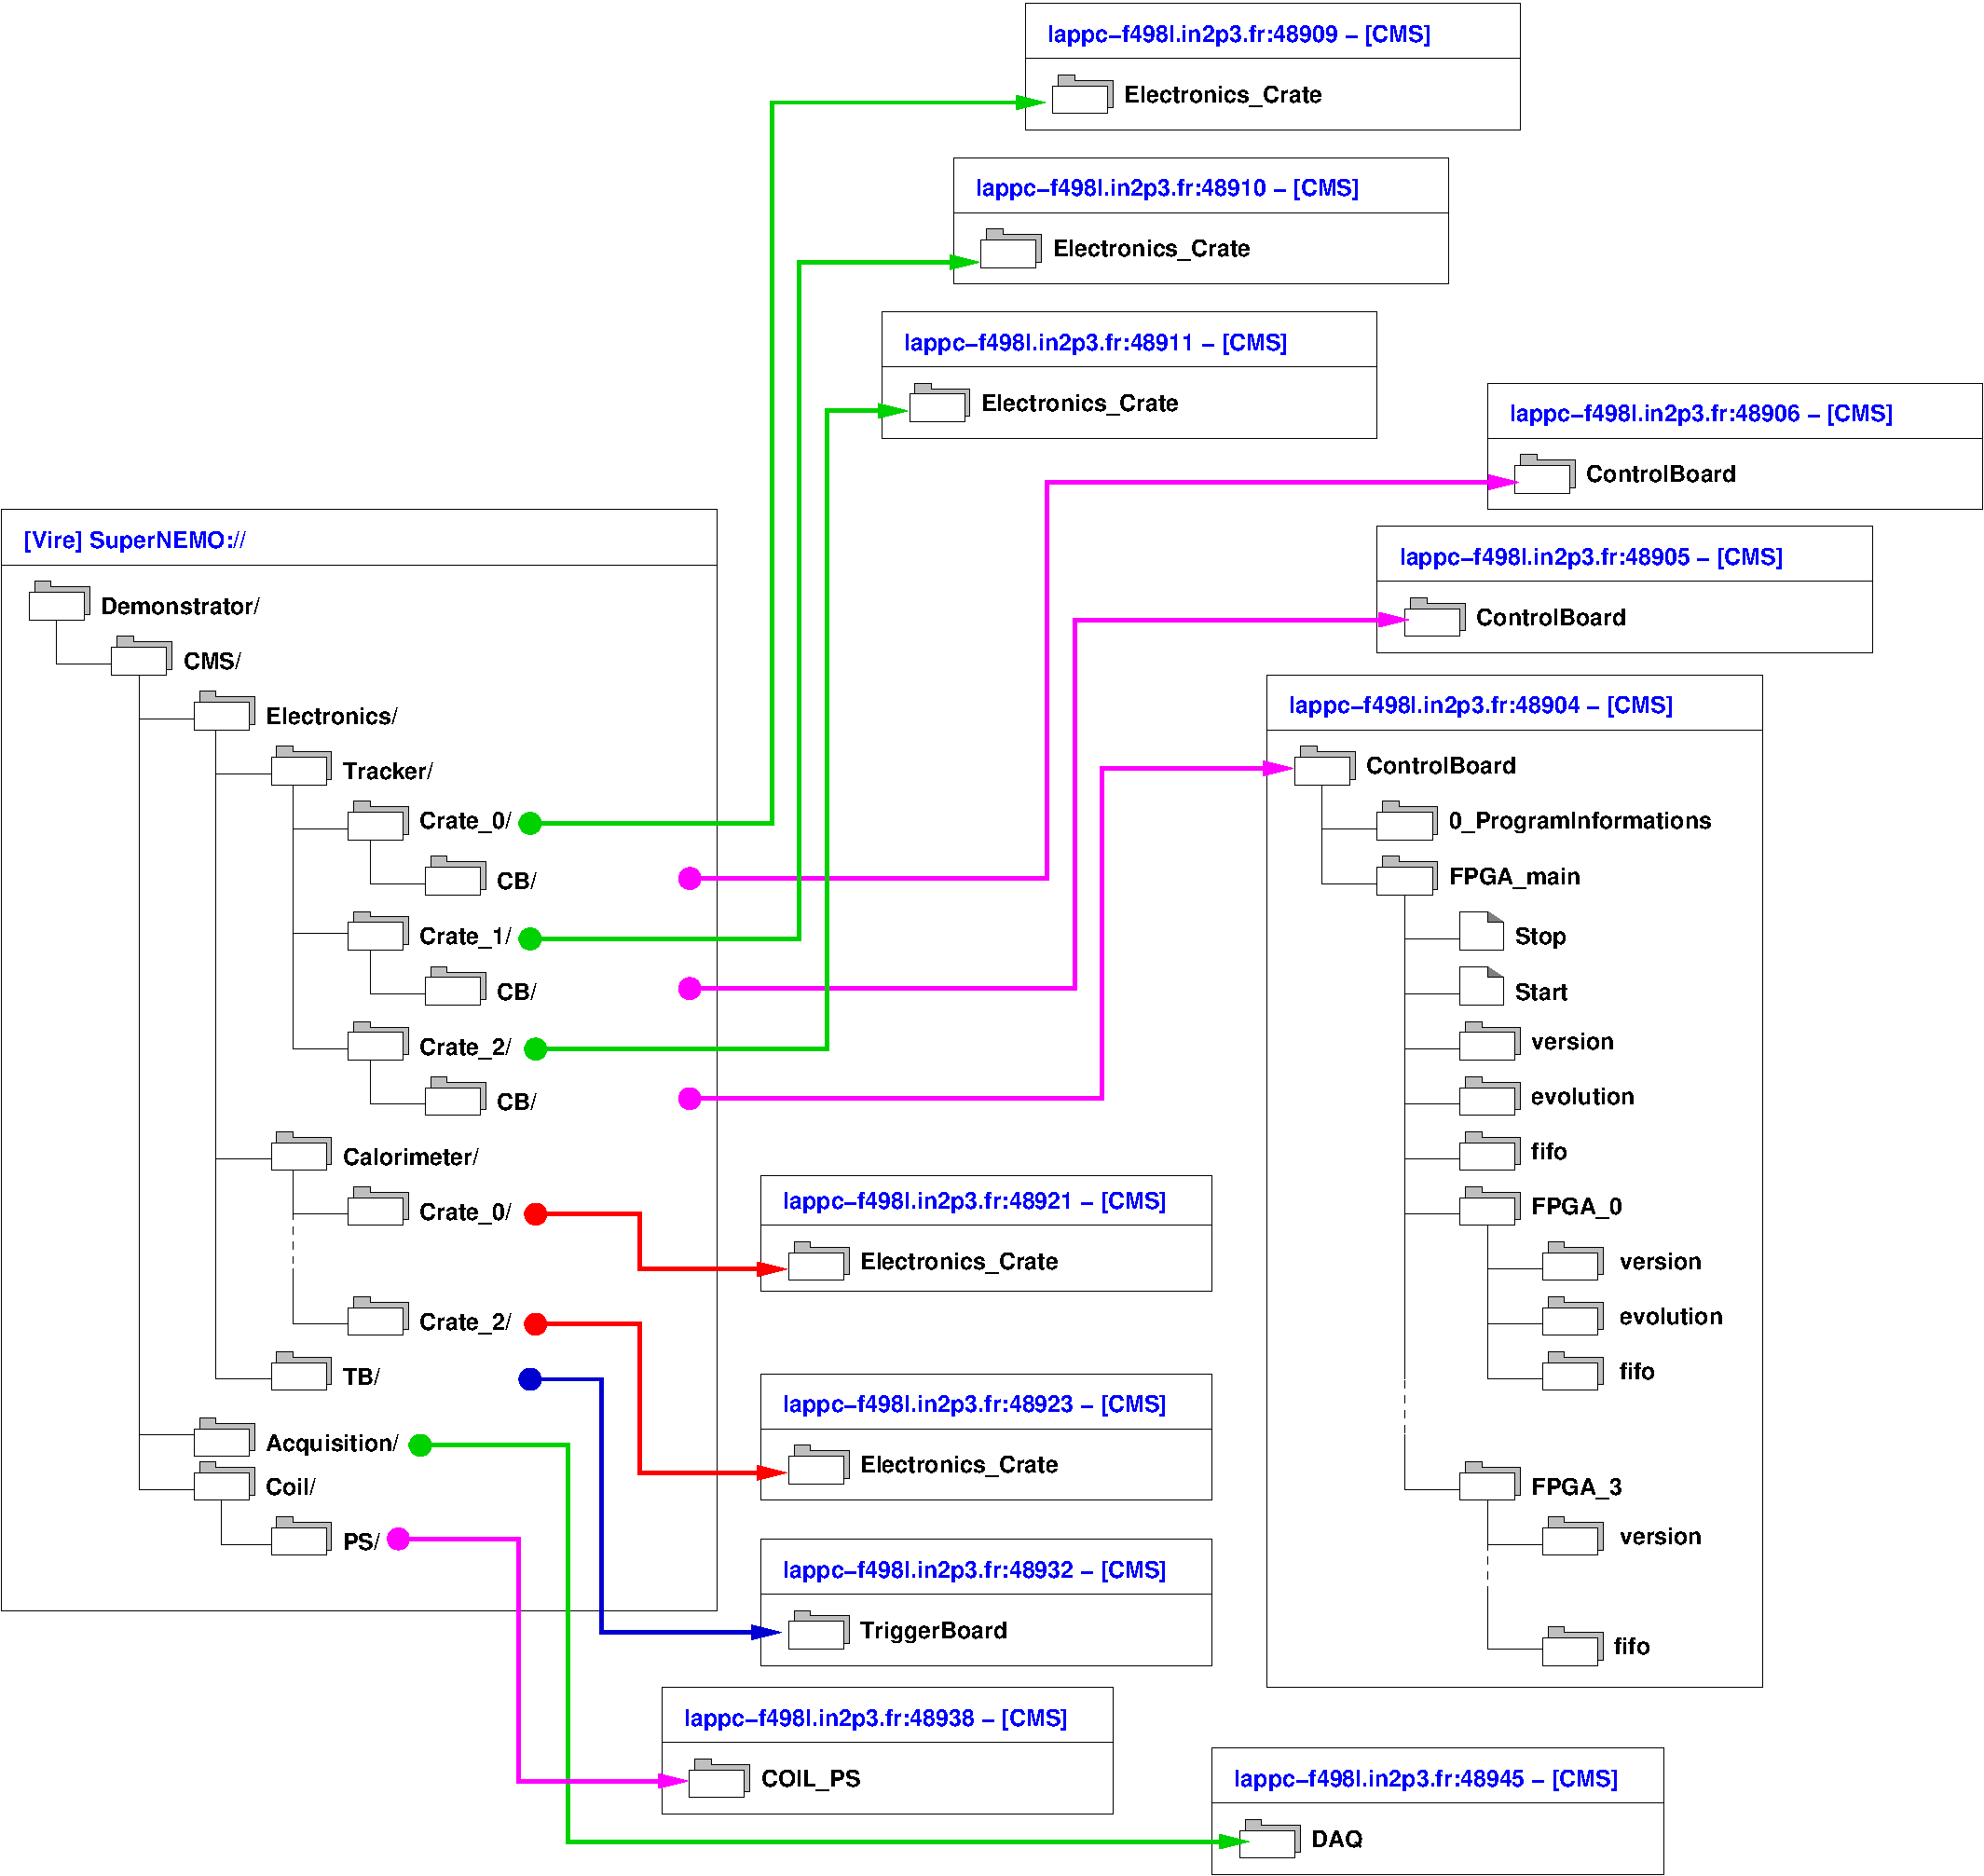
\includegraphics[width=\linewidth]{appendix/images/MOS_device_example_0.pdf}
\end{center}
\caption{The  mounting of  many  MOS device  hierarchies  in the  Vire
  device hierarchy.  Each OPCUA server  runs a simple  hardware device
  that is \emph{mounted} from a specific node with its own path.
%% of  devices described by the Vire API.
%%   The root device is named  \texttt{SuperNEMO:}.  The top level (root)
%%   device is  named \texttt{Demonstrator}. The devices  colored in blue
%%   are managed  through MOS/OPCUA. The  devices colored in  magenta are
%%   directly embedded in the Vire server.  Devices with the \texttt{dev}
%%   tag are typical  hardware device. Devices with  the \texttt{bot} tag
%%   are typical software devices.
}\label{fig:an:mos_dev_0}
\end{figure}




\subsection{Example}

Using  the examples  displayed  in  figure \ref{fig:an:mos_dev_0},  we
consider  in detail  the way  one specific  device managed  by MOS  is
mounted   in  the   Vire   hierarchy.  Figure   \ref{fig:an:mos_dev_3}
illustrates the mounting of a MOS device in Vire.

Here the Vire  server publishes the path of a  device representing the
control board  of the third  electronic crate  for the tracker  of the
SuperNEMO demonstrator module.  The full Vire path of this device is:

\textcolor{blue}{\texttt{SuperNEMO://Demonstrator/CMS/Electronics/Tracker/Crate\_2/CB}}

This is  the only Vire identifier  recognized by user to  address this
device.

On    the   figure,    one    can   see    that    the   MOS    server
\texttt{lappc−f498l.in2p3.fr} (port 48904) hosts a simple device which
is locally named \texttt{ControlBoard}.

When  mounting   this  device  in   the  Vire  hierarchy,   the  local
\texttt{[CMS]}  namespace and  \texttt{ControlBoard} device  names are
hidden and replaced by the Vire device path.  All daughter devices and
datapoints of  the \texttt{CMS/ControlBoard} device are  integrated as
daughters        of        the         Vire        device        named\\
\texttt{SuperNEMO://Demonstrator/CMS/Electronics/Tracker/Crate\_2/CB}.


For example, the \texttt{FPGA\_main} daughter device is now associated
to the following Vire path:

\textcolor{blue}{\texttt{SuperNEMO://Demonstrator/CMS/Electronics/Tracker/Crate\_2/CB/FPGA\_main/}}

and  its  \texttt{Stop} method  is  automatically  addressed with  the
following \emph{leaf} path:

\textcolor{blue}{\texttt{SuperNEMO://Demonstrator/CMS/Electronics/Tracker/Crate\_2/CB/FPGA\_main/Stop}}


\begin{figure}[h]
\begin{center}
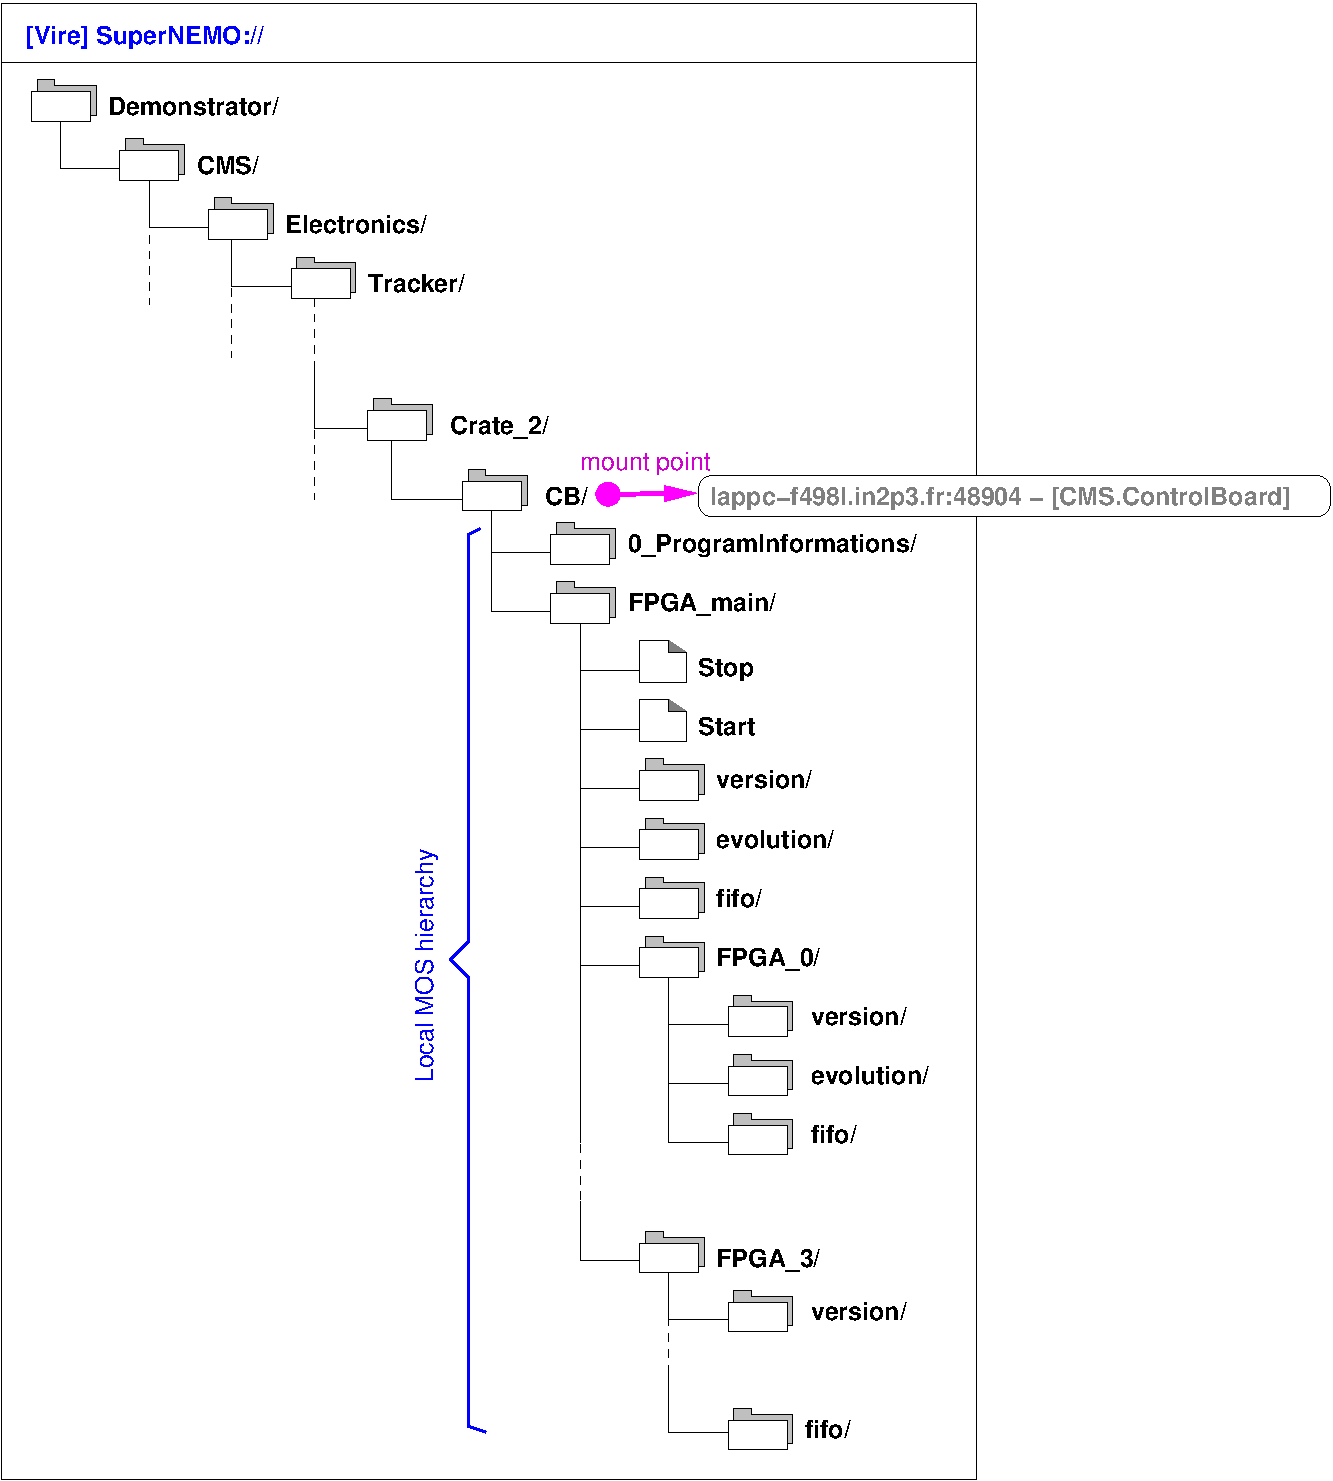
\includegraphics[width=0.8\linewidth]{appendix/images/MOS_device_example_3.pdf}
\end{center}
\caption{The  mounting of  one  MOS device and its local hierarchy  in the  Vire
  device hierarchy.}\label{fig:an:mos_dev_3}
\end{figure}



\subsection{Vire/MOS mapping}

As it can be  seen in the above example, the integration  of a new MOS
device in the Vire system is  achieved through soem kind of filesystem
mounting operation.   Particularly, it is  shown that the MOS  name of
the   mounted  root   device  is   replaced  by   an  arbitrary   Vire
path. However, all daughter  nodes (devices, datapoints) attached from
this root  node have their  relative MOS  names preserved in  the Vire
naming scheme.

Any  resource  (method)  associated  to any  of  such  daughter  nodes
inherits this relative naming scheme.

As Vire applications  describe resources through their  Vire paths, it
is thus needed to build an explicit map that associates resource paths
to MOS address  and name. The CMS  server will be able  to resolve the
MOS server/port and  embedded device associated to  the resource path.

The goal of the \texttt{devices\_launch.conf} file is not only to tell
the CMS server what MOS server should  be loaded and ran at start, but
also  to describe  the  \emph{mounting point/names}  used  by Vire  to
access the resources associated to MOS devices.  From the informations
stored in the  file, an explicit associative array must  be built when
the Vire server connect to the CMS server.  It will play the role of a
resource path resolver  when requests about resources will  be sent by
Vire applications.  This associative array  must be locked  during the
Vire/CMS connection.



%\subsubsection{Preparation of XML device models}

%% \noindent\underline{Pre-condition:}
%% The device is working and validated through the MOS/OPCUA server

%% \begin{enumerate}

%% \item Produce XML décrivant le modèle du device enrichi
%%   des metadata
%% Rédaction du fichier XML décrivant le modèle du device

%% \item Génération des fichiers model du type de device pour Vire

%% \item Génération des fichiers instances resolv.conf

%% \end{enumerate}


\vfill
\pagebreak
\clearpage

% end


\section{Vire messages}\label{app:vire_messages}

Within Vire  and between Vire  components and external  components, we
use  a communication  system  based on  Vire  messages.  This  section
describes the structure of such messages.

\subsection{General structure of a message}

Each message consists in two parts (figure \ref{fig-vire-message-message-cpp}):
\begin{itemize}

\item  the  \emph{header}  is   dedicated  to  generic  and  typicalle
  mandatory  informations  which  document   the  message  itself  and
  arbitrary high-level metadata.

\item  the \emph{body}  of the  message  contains the  real data: the payload.
  The structure of the message body depends on some convention. Vire uses
  its own convention to embed the payload data.

\end{itemize}

\begin{figure}[h]
\vskip 10pt
\small
\begin{Verbatim}[frame=single,xleftmargin=0.cm,label=\fbox{C++}]
struct vire::message::message {
  message_header header; // Header of the message
  message_body   body;   // Body of the message
};
\end{Verbatim}
\normalsize
\caption{The structure of a Vire message object (C++  class:
  \texttt{"vire::message::message"})}\label{fig-vire-message-message-cpp}
\end{figure}

\subsection{The message header}

The header contains (figure \ref{fig-vire-message-message_header-cpp}):
\begin{itemize}

  \item The mandatory \texttt{message\_id}  attribute is an identifier
    of the  message which  document the emitter  and a  unique message
    number.   Each emitter  is  responsible of  the  numbering of  the
    messages it  emits, typically using an  incremental technique. The
    message  number is  a positive  integer, starting  from 0  (figure
    \ref{fig-vire-message-message_identifier-cpp}).

  \item  The \texttt{timestamp}  attribute  encodes the  approximative
    time point when the message was  created. It contains the date and
    the time, using at least microsecond resolution.

    Typically,  with  JSON  encoding  system, it  is  expected  to  be
    formatted as a character string, using the following ISO format:

    \begin{center}
      \texttt{yyyymmddThhmmss.uuuuuu}
    \end{center}

    \noindent where:

    \vskip -10pt
    \begin{itemize}
    \item[\texttt{yyyymmdd} :] encodes year/month/day,
    \item[\texttt{hhmmssd} :] encodes hour/minute/second,
    \item[\texttt{uuuuuu} :] encodes microseconds.
    \end{itemize}

  \item   In   the   case    of   a   \emph{response}   message,   the
    \texttt{in\_reply\_to} attribute is set to identify the associated
    request message.

  \item  The \texttt{asynchronous}  boolean  attribute is  set if  the
    message processing  is explicitely requested  by the source  to be
    asynchronous (non-blocking).  In  RPC transactions, where requests
    are transmitted from one point to  the other, its default value is
    \emph{false}.   It  is possible  to  force  a RPC  transaction  in
    asynchronous mode.   This use  case is documented  elsewhere.  For
    event messaging, this flag is conventionally set to \emph{true}.

  \item  The  \texttt{body\_layout\_id}  attribute  is  the  mandatory
    identifier   of   the   layout   of  the   message   body   (class
    \texttt{"vire::utility::model\_identifier"}).  The  default layout
    for     message     body     inside    the     Vire     API     is
    \texttt{"vire::message::body\_format::typed\_payload"}, with version
    \texttt{"1.0"}                                             (figure
    \ref{fig-vire-utility-model_identifier-cpp}).

\end{itemize}


\begin{figure}[h]
\vskip 10pt
\small
\begin{Verbatim}[frame=single,xleftmargin=0.cm,label=\fbox{C++}]
struct vire::message::message_header {
  message_identifier message_id;     // Message identifier from the emitter.
  std::string        timestamp;      // Timestamp.
  message_identifier in_reply_to;    // Message identifier of the associated
                                     // request message (optional).
  bool               asynchronous,   // Asynchronous flag.
  vire::utility::model_identifier     body_layout_id; // Body layout identifier.
  std::map<std::string, std::string>  metadata;       // Key/value metadata dictionary.
};
\end{Verbatim}
\normalsize
\caption{The  structure  of  a   message  header  object  (C++  class:
  \texttt{"vire::message::message\_header"}).}\label{fig-vire-message-message_header-cpp}
\end{figure}

\begin{figure}[h]
\vskip 10pt
\small
\begin{Verbatim}[frame=single,xleftmargin=0.cm,label=\fbox{C++}]
struct vire::message::message_identifier {
  std::string emitter; // Name identifying the emitter of the message.
  int32_t     number;  // Number identifying the message in the emitter's
                       // message numbering scheme.
};
\end{Verbatim}
\normalsize
\caption{The      structure      of     a      message      identifier
  (C++  class:  \texttt{"vire::message::message\_identifier"}).}
\label{fig-vire-message-message_identifier-cpp}
\end{figure}

\begin{figure}[h]
\vskip 10pt
\small
\begin{Verbatim}[frame=single,xleftmargin=0.cm,label=\fbox{C++}]
struct vire::utility::model_identifier {
  std::string name;    // Name identifying the format of the message.
  std::string version; // String identifying the version of the format.
};
\end{Verbatim}
\normalsize
\caption{The structure of a model identifier (C++  class:  \texttt{"vire::utility::model\_identifier"}.}\label{fig-vire-utility-model_identifier-cpp}
\end{figure}




\begin{figure}[h]
\vskip 10pt
\small
\begin{Verbatim}[frame=single,xleftmargin=0.cm,label=\fbox{JSON}]
{
   "header" : {
      "message_id" : {
         "emitter" : "vire.server",
         "number" : 42
      },
      "timestamp" : "20160930T141408.413443",
      "in_reply_to" : {
         "initialized" : true,
         "value" : {
            "emitter" : "vire.client.0",
            "number" : 23
         }
      },
      "asynchronous" : false,
      "body_layout_id" : {
         "name" : "vire::message::body_format::typed_payload",
         "version" : {
            "initialized" : true,
            "value" : "1.0"
         }
      },
      "metadata" : [
         {
            "key" : "key1",
            "value" : "foo"
         },
         {
            "key" : "key2",
            "value" : "42"
         },
         {
            "key" : "key3",
            "value" : "3.1415899999999999"
         },
         {
            "key" : "key4",
            "value" : "true"
         }
      ]
   }
  "body" : {
      ...
   }
}
\end{Verbatim}
\normalsize
\caption{Example of  a   message  header  object in JSON format.}
\label{fig-vire-message-message_header-json}
\end{figure}

\vfill
\clearpage
\pagebreak

\subsection{The message body}

The    default    message   body    layout    in    Vire   is    named
\texttt{"vire::message::body\_format::typed\_payload"}        (version
\texttt{"1.0"}).   Each  message used  within  the  Vire framework  is
supposed to use this layout.  The general idea is that the body of the
message embeded the  \emph{payload object} that has  to be transmitted
between  two components  of  the system.   \emph{Payload objects}  are
classified in one of the three following categories:

\begin{enumerate}

\item \emph{Request}:  describes a request submitted  by one component
  to another component (generally during a synchronous RPC transaction).

\item  \emph{Response}: describes  the  response to  a former  request
  (generally during a synchronous RPC transaction).

\item \emph{Event}: describes an  arbitrary information record (alarm,
  exception, signal\dots) which is transmitted asynchronously.

\end{enumerate}

Vire implements the following class hierarchy:

\begin{center}
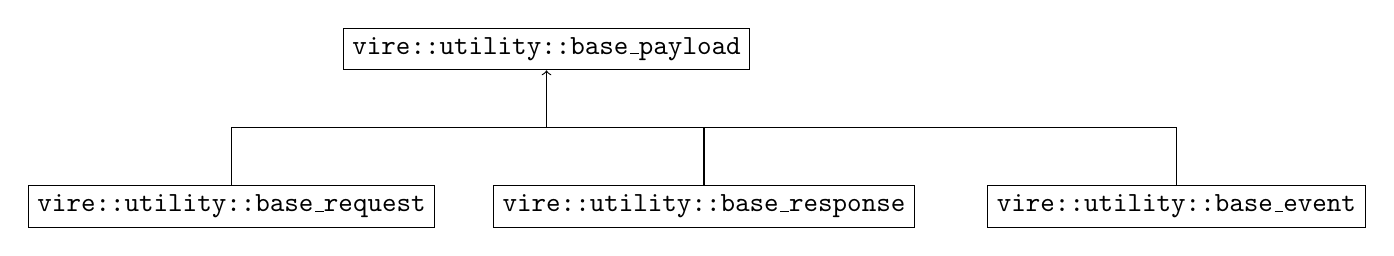
\begin{tikzpicture}
  \node (payload)  at (0,2)  [draw] {\texttt{vire::utility::base\_payload}};
  \node (request)  at (-4,0) [draw] {\texttt{vire::utility::base\_request}};
  \node (response) at (2,0)  [draw] {\texttt{vire::utility::base\_response}};
  \node (event)    at (8,0)  [draw] {\texttt{vire::utility::base\_event}};

  %\draw[style=help lines] (-3,-1) grid (10,4);
  \draw (node cs:name=response,anchor=north) |- (0,1);
  \draw (node cs:name=event,anchor=north)    |- (0,1);
  \draw[->] (node cs:name=request,anchor=north)
  |- (0,1) -| (node cs:name=payload,anchor=south);
\end{tikzpicture}
\end{center}

The requirements for the transmitted object are the following:

\begin{itemize}

\item The  type of the object  must be conventionally associated  to a
  unique     \emph{model      identifier}     object      (see     the
  \texttt{"vire::utility::model\_identifier"} class)  which contains a
  unique   name   (\textit{string    identifier})   and   possibly   a
  \textit{version identifier}.  Each software  component that may send
  or  receive the  object  should agree  on  this type  identification
  scheme.   This   enable  the  use  of   object  factories,  whatever
  programming  langage  is used  on  both  side of  the  communication
  system.

\item  For each  software component,  the object  type must  have some
  dedicated  encoding/decoding  functions  available  (again  whatever
  programming language is used). For example the Vire API supports the
  following encoding formats:

  \begin{itemize}

  \item JSON (MIME  encoding type: \texttt{"application/x-json"}), which
    is supportable by many languages,

  \item  Protobuf  (Google  Protocol   Buffers,  MIME  encoding  type:
    \texttt{"application/x-protobuf"}), which is also widely supported,

  \item   Boost/serialisation   (XML,    text   or   binary   archives
    \texttt{"application/x-boost-serialization-xml"},
    \texttt{"application/x-boost-serialization-text"},
    \texttt{"application/x-boost-serialization-binary"}),    which    in
    principle is supported by C++ only.

  \end{itemize}

  The Protobuf  encoding format will be  used to serialize/deserialize
  the  Vire  messages transported  between  the  Vire server  and  the
  CMS/LAPP server.

\end{itemize}

Vire uses a dedicated layout to represent the body of any message with
its embedded payload object. With this technique, the structure of the
body          contains         two          attributes         (figure
\ref{fig-app-vire-message-message_body-cpp}):

\begin{enumerate}

\item The \texttt{payload\_type\_id} specifies the type of the payload
  object   (figure   \ref{fig-app-vire-utility-model_identifier-cpp}).
  This unique name  is conventionaly fixed for a  given application. A
  version tag allows to support possible evolution of the object type.

\item The  \texttt{payload} is a  handle to  a payload object  of type
  request, response or event.

  %% \begin{itemize}
  %% \item Within  the producer  component of  the message,  the encoding
  %%   function associated to the object  type is responsible to generate
  %%   the JSON stream for the object and store it in the buffer.

  %% \item Within  the consumer  component of  the message,  the decoding
  %%   function associated to the object type is responsible to parse the
  %%   JSON stream stored in the buffer and restore the object in memory.

  %% \end{itemize}

  It is expected  that, on both sides of the  connection, the software
  components can  access dedicated  software plugins which  ensure the
  support  of  various   \emph{payload  object  types}  conventionnaly
  associated  with  their  \emph{payload type  identifiers}  and  also
  providing JSON and/or Protobuf encoding/decoding functionalities.

  %% The   system  allows  to  support
  %% modification  in the  structure of  the objects  thanks to  version
  %% tagging.

\end{enumerate}

\begin{figure}[h]
\vskip 10pt
\small
\begin{Verbatim}[frame=single,xleftmargin=0.cm,label=\fbox{C++}]
struct message_body {
  vire::utility::model_identifier     payload_type_id; // Object type identifier.
  const vire::utility::base_payload * payload;         // Handle to a payload object.
};
\end{Verbatim}
\normalsize
\caption{The structure of a message body object (C++).}
\label{fig-app-vire-message-message_body-cpp}
\end{figure}

\begin{figure}[h]
\vskip 10pt
\small
\begin{Verbatim}[frame=single,xleftmargin=0.cm,label=\fbox{JSON}]
{
  "header" : {
    ...
  },
  "body" : {
    "payload_type_id" : {
      "name" : "vire::message::testing::error_event",
      "version" : {
        "initialized" : false
      }
    },
    "payload" : {
      "timestamp" : "20160930T141743.759085"
      "err" : {
        "code" : 3,
        "message" : "A basic error"
      },
    }
  }
}
\end{Verbatim}
\normalsize
\caption{Example of  a   message  body  object in JSON format.}
\label{fig-vire-message-message_body-json}
\end{figure}

\vfill
\clearpage
\pagebreak

% end

%\input{appendix/app_json_fmt.tex}

\section{The \emph{Protocol Buffers} format}\label{app:protobuf_fmt}

\subsection{Introduction}

The  Google  Protocol Buffers  (\emph{protobuf})  library  is used  to
represent the objects that are exchanged between the Vire clients, the
Vire server and the CMS server.  The  version 3 of the format is used,
implying   at   least   version   3.0.0  (September   2016)   of   the
\emph{protobuf} library.

Each  data   structure  of  interest   can  be  described   through  a
\texttt{.proto}  file  from  which  stub files  can  be  automatically
generated  with the  \texttt{protoc} compiler.  For Vire  and its  CMS
interface, the C++ and Java programming languages will be used.


A  collection of  \texttt{.proto}  files are  provided  with the  Vire
library to represent all kind  of data structures transferable between
networked agents  (Vire server,  Vire clients, CMS/LAPP  server).  The
objects of  the highest level  are named \emph{payload  objects} (like
\emph{request},  \emph{response} and  \emph{event} objects).   They
are composed of attributes of more basic data structures.

\subsection{Example}

The following  class diagram  illustrates two data  structures defined
within the Vire library with an inheritance relationship between them.

\begin{center}
  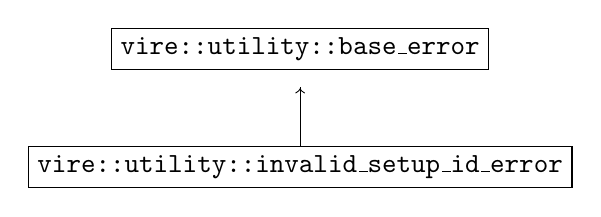
\begin{tikzpicture}
    \node (base)     at (0,1.5)  [draw] {\texttt{vire::utility::base\_error}};
    \node (setup)    at (0,0)  [draw] {\texttt{vire::utility::invalid\_setup\_id\_error}};

    \draw[->]   (node cs:name=setup,anchor=north) |- (0,1);
    |- (0,1) -| (node cs:name=base,anchor=south);
  \end{tikzpicture}
\end{center}

The \texttt{vire::utility::base\_error}  is the  parent class  for all
\emph{error}  objects.   It  contains   two  attributes:   an  integer
\emph{error code}  and a  character string describing  the \emph{error
  message}.

The   \texttt{vire::utility::invalid\_setup\_id\_error}  class   is  a
specialized error class  which represents explicitely an  error due to
an identification  failure of  the experimental setup.   It implements
additional mutually exclusive attributes: the \emph{unrecognized name}
of the setup or the \emph{unrecognized version} of the setup.

This   example  illustrates   the  protobuf   representation  of   the
\texttt{vire::utility::base\_error}  in the  Vire  library, using  the
\texttt{"vire/utility/BaseError.proto"} file:

\small
\begin{Verbatim}[frame=single,xleftmargin=0.cm,label=\fbox{protobuf}]
  syntax = "proto3";
  package vire.utility; // Namespace

  message BaseError {

    // reserved 1; // Reserved for _base message

    // Attributes:
    int32  code           = 100; // The error code
    string message_format = 101; // The error description message

  }
\end{Verbatim}
\normalsize

\vfill
\clearpage
\pagebreak

\subsection{Vire protobuf conventions}

Vire uses the following conventions:

\begin{enumerate}

\item
  The member index  \texttt{1} is reserved to represent the  link of a
  class to its main base/parent class (if any).  It is not used if the
  data structure does not inherit any data structure.
  If a data structure naturally inherits another one, it is thus possible
  to  represent the  inheritance  relationship as  illustrated with  the
  \texttt{"vire/utility/InvalidSetupIdError.proto"}      file      which
  represents the \texttt{vire::utility::invalid\_setup\_id\_error} class
  in the Vire library:

  \small
  \begin{Verbatim}[frame=single,xleftmargin=0.cm,label=\fbox{protobuf}]
    syntax = "proto3";
    package vire.utility; // Namespace

    import "vire/utility/BaseError.proto"; // Dependency

    message InvalidSetupIdError {

      BaseError _base = 1; // The base class

      // Additional attributes:
      oneof detail { // Mutual exclusion
        string invalid_setup_name    = 100; // The failed setup name
        string invalid_setup_version = 101; // The failed setup version
      }

    }
  \end{Verbatim}
  \normalsize

\item The  \texttt{\_base} member  is conventionally  used to  represent the
  inheritance   relationship    from   a   data   structure    of   type
  \texttt{"vire.utility.BaseError"}.

\item Member indexes from \texttt{2}  to \texttt{99} are also reserved
  for possible future usage (multiple inheritance, metadata\dots).

\item
  The first member of the data structure must start at index \texttt{100}.

\end{enumerate}

\vfill
\clearpage
\pagebreak

% end


\section{Vire payload objects}\label{app:payload}

\subsection{Introduction}

As  mentioned in  appendix \ref{app:protobuf_fmt},  Vire messages  are
wrappers for \emph{payload objects}.  Each  type of payload object can
be represented  through the \emph{protobuf} mechanism.   The following
class hierarchy shows the base architecture used to define new payload
objects.

\begin{center}
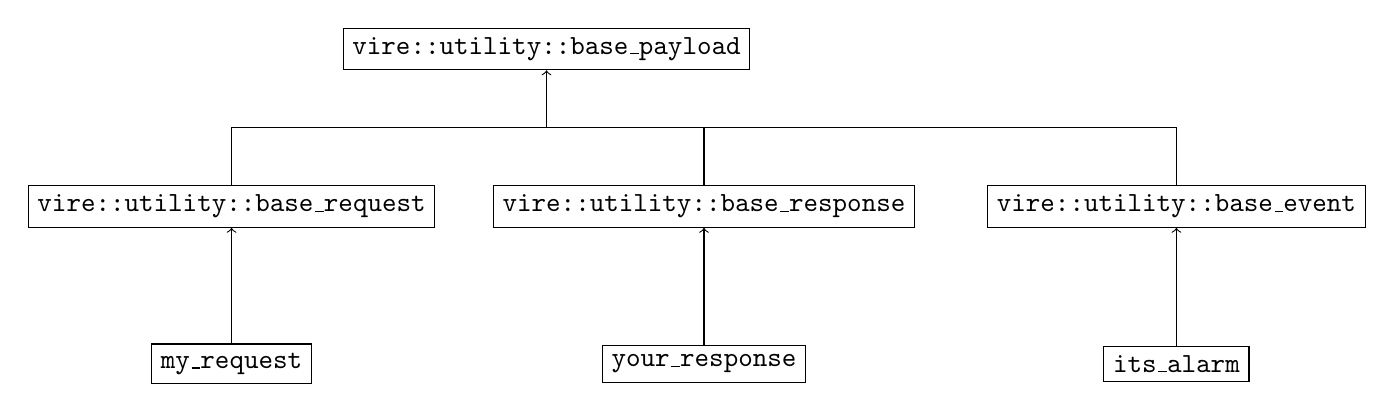
\begin{tikzpicture}
  \node (payload)  at (0,2)   [draw] {\texttt{vire::utility::base\_payload}};
  \node (request)  at (-4,0)  [draw] {\texttt{vire::utility::base\_request}};
  \node (response) at (2,0)   [draw] {\texttt{vire::utility::base\_response}};
  \node (event)    at (8,0)   [draw] {\texttt{vire::utility::base\_event}};
  \node (my)       at (-4,-2) [draw] {\texttt{my\_request}};
  \node (your)     at (2,-2)  [draw] {\texttt{your\_response}};
  \node (its)    at (8,-2)    [draw] {\texttt{its\_alarm}};

  %\draw[style=help lines] (-6,-2) grid (10,2);
  \draw (node cs:name=response,anchor=north) |- (0,1);
  \draw (node cs:name=event,anchor=north)    |- (0,1);
  \draw[->] (node cs:name=request,anchor=north)
  |- (0,1) -| (node cs:name=payload,anchor=south);
  \draw[->] (node cs:name=my,anchor=north)
  |- (-4,-1) -| (node cs:name=request,anchor=south);
  \draw[->] (node cs:name=your,anchor=north)
  |- (2,-1) -| (node cs:name=response,anchor=south);
  \draw[->] (node cs:name=its,anchor=north)
  |- (8,-1) -| (node cs:name=event,anchor=south);
\end{tikzpicture}
\end{center}


\begin{center}
\vskip 10pt
\small
\begin{tabular}{|l|l|l|}
  \hline
  \textbf{Vire C++ class} & \textbf{protobuf message type} & \textbf{protobuf definition file} \\
  \hline
  \hline
  \multicolumn{3}{|c|}{\emph{general types}} \\
  \hline
  boost::posix\_time::ptime & google.protobuf.Timestamp & google/protobuf/timestamp.proto \\
  \hline
  \hline
  \multicolumn{3}{|c|}{\emph{identifier types}} \\
  \hline
  vire::utility::base\_identifier & vire.utility.Baseidentifier & vire/utility/Baseidentifier.proto \\
  \hline
  vire::utility::instance\_identifier & vire.utility.InstanceIdentifier & vire/utility/InstanceIdentifier.proto \\
  \hline
  vire::utility::model\_identifier & vire.utility.ModelIdentifier & vire/utility/ModelIdentifier.proto \\
  \hline
  \hline
  \multicolumn{3}{|c|}{\emph{error types}} \\
  \hline
  vire::utility::base\_error & vire.utility.BaseError & vire/utility/BaseError.proto \\
  \hline
  vire::utility::invalid\_context\_error & vire.utility.InvalidContextError & vire/utility/InvalidContextError.proto \\
  \hline
  vire::utility::invalid\_setup\_id\_error & vire.utility.InvalidSetupIdError & vire/utility/InvalidSetupIdError.proto \\
  \hline
  \hline
  \multicolumn{3}{|c|}{\emph{payload types}} \\
  \hline
  vire::utility::base\_payload & vire.utility.BasePayload & vire/utility/BasePayload.proto \\
  \hline
  vire::utility::base\_request & vire.utility.BaseRequest & vire/utility/BaseRequest.proto \\
  \hline
  vire::utility::base\_response & vire.utility.BaseResponse & vire/utility/BaseResponse.proto \\
  \hline
  vire::utility::base\_event & vire.utility.BaseEvent & vire/utility/BaseEvent.proto \\
  \hline
  vire::utility::base\_alarm & vire.utility.BaseAlarm & vire/utility/BaseAlarm.proto \\
  \hline
  \hline
  \multicolumn{3}{|c|}{\emph{messenging types}} \\
  \hline
  vire::message::message\_identifier & vire.message.MessageIdentifier & vire/message/MessageIdentifier.proto \\
  \hline
  vire::message::msg\_header & vire.message.MsgHeader & vire/message/MsgHeader.proto \\
  \hline
  vire::message::msg\_body & vire.message.MsgBody & vire/message/MsgBody.proto \\
  \hline
  vire::message::message & vire.message.Message & vire/message/Message.proto \\
  \hline
\end{tabular}
\normalsize
\end{center}


\begin{center}
\vskip 10pt
\small
\begin{tabular}{|l|l|l|}
  \hline
  \multicolumn{3}{|c|}{\emph{Resource management related types}} \\
  \hline
  vire::cms::resource\_status\_record & vire.cms.ResourceStatusRecord & vire/cms/ResourceStatusRecord.proto \\
  \hline
  vire::cms::resource\_fetch\_status\_request & vire.cms.ResourceFetchStatusRequest & vire/cms/ResourceFetchStatusRequest.proto \\
  \hline
  vire::cms::resource\_fetch\_status\_success\_response & vire.cms.ResourceFetchStatusSuccessResponse & vire/cms/ResourceFetchStatusSuccessResponse.proto \\
  \hline
  vire::cms::resource\_fetch\_status\_failure\_response & vire.cms.ResourceFetchStatusFailureResponse & vire/cms/ResourceFetchStatusFailureResponse.proto \\
  \hline
  vire::cms::resource\_exec\_request & vire.cms.ResourceExecRequest & vire/cms/ResourceExecRequest.proto \\
  \hline
  vire::cms::resource\_exec\_success\_response & vire.cms.ResourceExecSuccessResponse & vire/cms/ResourceExecSuccessResponse.proto \\
  \hline
  vire::cms::resource\_exec\_failure\_response & vire.cms.ResourceExecFailureResponse & vire/cms/ResourceExecFailureResponse.proto \\
  \hline
  vire::cms::resource\_exec\_non\_blocking\_request & vire.cms.ResourceExecNonBlockingRequest & vire/cms/ResourceExecNonBlockingRequest.proto \\
  \hline
  vire::cms::resource\_exec\_non\_blocking\_ack\_response & vire.cms.ResourceExecNonBlockingAckResponse & vire/cms/ResourceExecNonBlockingAckResponse.proto \\
  \hline
  vire::cms::resource\_exec\_non\_blocking\_noack\_response & vire.cms.ResourceExecNonBlockingNoackResponse & vire/cms/ResourceExecNonBlockingNoackResponse.proto \\
  \hline
  vire::cms::resource\_exec\_non\_blocking\_success\_event & vire.cms.ResourceExecNonBlockingSuccessEvent & vire/cms/ResourceExecNonBlockingSuccessEvent.proto \\
  \hline
  vire::cms::resource\_exec\_non\_blocking\_failure\_event & vire.cms.ResourceExecNonBlockingFailureEvent & vire/cms/ResourceExecNonBlockingFailureEvent.proto \\
  \hline
  vire::cms::resource\_exec\_error & vire.cms.ResourceExecError & vire/cms/ResourceExecError.proto \\
  \hline
  vire::cms::invalid\_status\_error & vire.cms.ResourceExecError & vire/cms/ResourceExecError.proto \\
  \hline
  %% vire::cms::invalid\_credentials\_error & vire.cms.InvalidCredentialsError & vire/cms/InvalidCredentialsError.proto \\
  %% \hline
  %% vire::cms::invalid\_user\_error & vire.cms.InvalidUserError & vire/cms/InvalidUserError.proto \\
  %% \hline
  vire::cms::invalid\_resource\_error & vire.cms.InvalidUserError & vire/cms/InvalidUserError.proto \\
  \hline
  vire::cms::no\_pubsub\_resource\_error & vire.cms.NoPubsubResourceError & vire/cms/NoPubsubResourceError.proto \\
  \hline
  \hline
  \multicolumn{3}{|c|}{\emph{Resource pub/sub management types}} \\
  \hline
  vire::cms::resource\_pubsub\_subscribe\_request & vire.cms.ResourcePubsubSubscribeRequest & vire/cms/ResourcePubsubSubscribeRequest.proto \\
  \hline
  vire::cms::resource\_pubsub\_subscribe\_success\_response & vire.cms.ResourcePubsubSubscribeRSuccessResponse & vire/cms/ResourcePubsubSubscribeRSuccessResponse.proto \\
  \hline
  vire::cms::resource\_pubsub\_subscribe\_failure\_response & vire.cms.ResourcePubsubSubscribeRFailureResponse & vire/cms/ResourcePubsubSubscribeRSuccessResponse.proto \\
  \hline
  \hline
  \multicolumn{3}{|c|}{\emph{Vire/CMS server interface types}} \\
  \hline
  vire::cmsinterface::connection\_request & vire.cmsinterface.ConnectionRequest & vire/cmsinterface/ConnectionRequest.proto \\
  \hline
  vire::cmsinterface::connection\_success\_response & vire.cmsinterface.ConnectionSuccessResponse & vire/cmsinterface/ConnectionSuccessResponse.proto \\
  \hline
  vire::cmsinterface::connection\_failure\_response & vire.cmsinterface.ConnectionFailureResponse & vire/cmsinterface/ConnectionFailureResponse.proto \\
  \emph{embedded:} unknown\_resources\_error & .UnknownResourcesError &  \\
  \hline
  vire::cmsinterface::disconnection\_request & vire.cmsinterface.DisconnectionRequest & vire/cmsinterface/DisconnectionRequest.proto \\
  \hline
  vire::cmsinterface::disconnection\_success\_response & vire.cmsinterface.DisconnectionSuccessResponse & vire/cmsinterface/DisconnectionSuccessResponse.proto \\
  \hline
  %% \hline
  %% vire::cmsinterface::disconnection\_failure\_response & vire.cmsinterface.DisconnectionFailureResponse & vire/cmsinterface/DisconnectionFailureResponse.proto \\
\end{tabular}
\normalsize
\end{center}

\subsection{Basic data structures}

Any  payload object  (request, response  or event)  generally contains
some information records which are  specific to the functionalities of
the  payload  object they  belong.   These  records are  of  arbitrary
types. Of course they should be  translatable in terms of the protobuf
library.
%Of course they can be (de)serialized using JSON.
Some of these types are very  general and defined within the Vire core
API itself because they are reused by various payload objects not only
through  the Vire-CMS/LAPP  interface  but also  between  Vire clients  and
servers, independently  of the  CMS/LAPP server.  However,  the use  of the
Protocol Buffers interface makes possible  to publish the interface of
such data to the outside world, including the CMS/LAPP server in priority.

%% Other one are specific to the Vire/CMS interface and thus managed only
%% in the \texttt{Vire\_CMSInterface} API.
These  types  are considered  as  \emph{basic}.  Among them  we  find:
generic error  types, generic  identifier types,  timestamps, resource
status records\dots We propose to describe them in this section.

Once a sufficient collection of  basic data record types is available,
it  is possible  to describe  high  level payload  object types  which
aggregate attributes of such types.

Other record  types are specific to  some payload objects and  will be
never  used outside  the scope  of these  payload objects.   Such data
structures will be  explicitely declared with the  payload object they
belong to, likely as embedded types/classes.


\subsubsection{Errors}

Some  \emph{response} or  \emph{event} payload  objects may  contain a
specific  error  record  object.   A  \emph{failure  response}  or  an
\emph{exception  event}  object will  generally  embed  such an  error
record object.

Each  \emph{error record}  is represented  by an  instance of  a given
error type.   Each of  the error  types defined  in Vire  inherits the
\texttt{vire::utility::base\_error}      base       class      (figure
\ref{fig-app-payload-base_error})   which   contains   the   following
attributes:

\begin{itemize}

\item the error code: A non zero  integer which is set to 1 by default
  (indicating  a  generic  failure  case).   The  error  code  can  be
  conventionally  set to  any positive  integer value  to represent  a
  specific error case, depending on the context.

\item the error  message: an optional human  readable character string
  which documents the error as usefully as possible.

\end{itemize}

\begin{figure}[h]
\vskip 10pt
\small
\begin{Verbatim}[frame=single,xleftmargin=0.cm,label=\fbox{C++}]
struct vire::utility::base_error
{
  // Attributes:
  int         code;           // Error code (>0).
  std::string message_format; // Error message (optional).
};
\end{Verbatim}
\normalsize
\caption{The structure of a \texttt{"vire::utility::base\_error"} object
  (C++).}
\label{fig-app-payload-base_error}
\end{figure}


%% An example of JSON formatted basic error object is given in figure
%% \ref{fig-app-payload-base_error-1}.
%%
%% \begin{figure}[h]
%% \vskip 10pt
%% \small
%% \begin{Verbatim}[frame=single,xleftmargin=0.cm,label=\fbox{\texttt{JSON}}]
%% {
%%   "code" : "42",
%%   "message_format" : "Invalid AMQP server port=[2341]"
%% }
%% \end{Verbatim}
%% \normalsize
%% \caption{JSON  formatted  basic  error  object  (class
%%   \texttt{vire::utility::base\_error}.}
%% \label{fig-app-payload-base_error-1}
%% \end{figure}

Several type of generic errors are defined in Vire:


\begin{center}
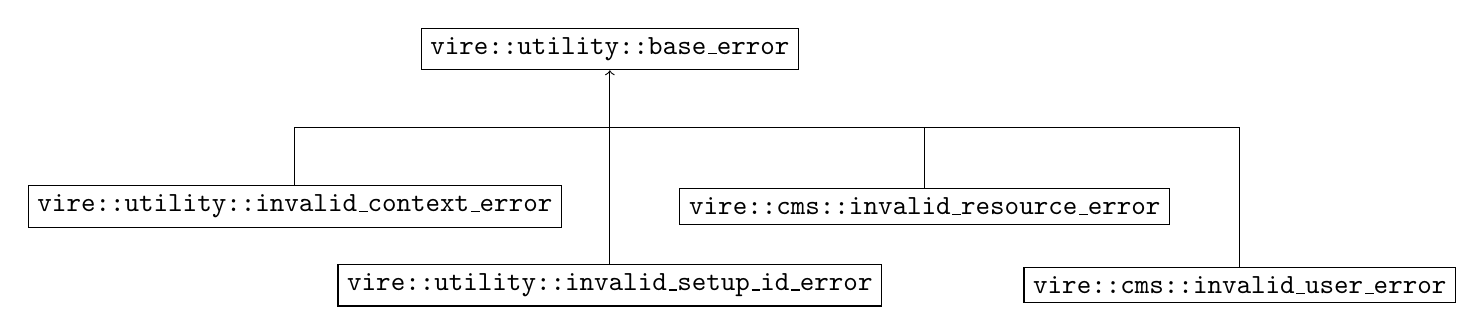
\begin{tikzpicture}
  \node (base)     at (0,2)  [draw] {\texttt{vire::utility::base\_error}};
  \node (context)  at (-4,0) [draw] {\texttt{vire::utility::invalid\_context\_error}};
  \node (setup)    at (0,-1)  [draw] {\texttt{vire::utility::invalid\_setup\_id\_error}};
  \node (resource) at (4,0)  [draw] {\texttt{vire::cms::invalid\_resource\_error}};
  \node (user)     at (8,-1)  [draw] {\texttt{vire::cms::invalid\_user\_error}};

  \draw     (node cs:name=setup,anchor=north)    |- (0,1);
  \draw     (node cs:name=resource,anchor=north) |- (0,1);
  \draw     (node cs:name=user,anchor=north)     |- (0,1);
  \draw[->] (node cs:name=context,anchor=north)
  |- (0,1) -| (node cs:name=base,anchor=south);
\end{tikzpicture}
\end{center}

\noindent
Here are a few error object types defined in Vire.  Some types belongs
to the \texttt{utility} namespace, other  ones are in the \texttt{cms}
namespace:

\begin{itemize}

\item \texttt{"vire::utility::invalid\_context\_error"} : occurs typically when
  the general context of the execution of a given resource is not adapted.\\
  It is mapped to the \texttt{"vire.utility.InvalidContextError"} protobuf record.

\item \texttt{"vire::utility::invalid\_setup\_id\_error"} : occurs in case
  of an invalid identification of the experimental setup managed
  by the Vire or CMS server.\\
  It is mapped to the \texttt{"vire.utility.InvalidSetupIdError"} protobuf record.

\item \texttt{"vire::cms::invalid\_resource\_error"} : occurs in case
  of an invalid identification of a resource.\\
  It is mapped to the  \texttt{"vire.cms.InvalidResourceError"} protobuf record.

\item \texttt{"vire::cms::invalid\_status\_error"}: occurs when an attempt
  to access a resource that has not the proper status.\\
  It is mapped to the  \texttt{"vire.cms.InvalidStatusError"} protobuf record.

\item \texttt{"vire::cms::invalid\_user\_error"} : occurs in case
  of an invalid identification of an user.\\
  It is mapped to the  \texttt{"vire.cms.InvalidUserError"} protobuf record.

\item \texttt{"vire::cms::invalid\_credentials\_error"} : occurs in case
  of user authentication error.\\
  It is mapped to the  \texttt{"vire.cms.InvalidCredentialsError"} protobuf record.

\item \texttt{"vire::cms::resource\_exec\_error"} : occurs in case
  of error at the execution of a given resource.\\
  It is mapped to the  \texttt{"vire.cms.ResourceExecError"} protobuf record.

\end{itemize}



\subsubsection{Object and type identifiers}

Vire  uses  some dedicated  classes  to  represent the  identifier  of
various objects  (or \emph{instances})  as well  as various  types (or
\emph{models})  of components.  Vire  implements  the following  class
hierarchy:

\begin{center}
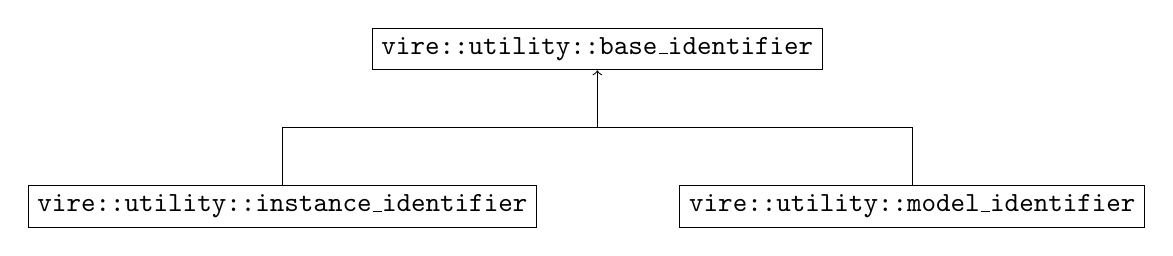
\begin{tikzpicture}
  \node (base)  at (0,2)  [draw] {\texttt{vire::utility::base\_identifier}};
  \node (instance)  at (-4,0) [draw] {\texttt{vire::utility::instance\_identifier}};
  \node (model) at (4,0)  [draw] {\texttt{vire::utility::model\_identifier}};

  \draw (node cs:name=model,anchor=north) |- (0,1);
\draw[->] (node cs:name=instance,anchor=north)
  |- (0,1) -| (node cs:name=base,anchor=south);
\end{tikzpicture}
\end{center}

The          \texttt{vire::utility::base\_identifier}          (figure
\ref{fig-app-payload-base_identifier}) class is  a pure abstract class
that cannot be instantiated. However  it contains a mandatory name and
an  optional  version description  which  are  used by  all  inherited
classes:

\begin{itemize}

\item The   \texttt{vire::utility::instance\_identifier}    concrete   class
inherits  \texttt{vire::utility::base\_identifier}  and   is  used  to
identify \underline{unique instances of objects} known by the system.

\item The  \texttt{vire::utility::model\_identifier}   concrete  class  also
inherits  \texttt{vire::utility::base\_identifier}  and   is  used  to
identify \underline{types of objects} registered in the system.

\end{itemize}

The only difference between these two classes is the validation scheme
of  the name  attribute.

\begin{figure}[h]
\vskip 10pt
\small
\begin{Verbatim}[frame=single,xleftmargin=0.cm,label=\fbox{C++}]
struct base_identifier
{
  // Attributes:
  std::string name;    // The mandatory name uniquely identifying the object or
                       // the type of object.
  std::string version; // An optional character string representing the version
                       // of the object type.
};
\end{Verbatim}
\normalsize
\caption{The structure of the \texttt{vire::utility::base\_identifier}
  class (C++).}
\label{fig-app-payload-base_identifier}
\end{figure}

%%  Figure  \ref{fig-app-payload-identifier-json}
%% shows an example of instance indentifier.
%% \begin{figure}[h]
%% \vskip 10pt
%% \small
%% \begin{Verbatim}[frame=single,xleftmargin=0.cm,label=\fbox{\texttt{JSON}}]
%% {
%%   "name" : "vire::resource::invalid_resource_error",
%%   "version" : "1.0"
%% }
%% \end{Verbatim}
%% \normalsize
%% \caption{JSON  formatted class identifier  object (class
%%   \texttt{vire::utility::model\_identifier}).   Here one  identifies a
%%   specific error type.}
%% \label{fig-app-payload-identifier-json}
%% \end{figure}


\vfill
\pagebreak
\clearpage

\subsubsection{Resource related objects}

\begin{itemize}

\item
Class \texttt{vire::cms::invalid\_resource\_error} (figure \ref{fig-app-payload-invalid_resource_error}).

\begin{center}
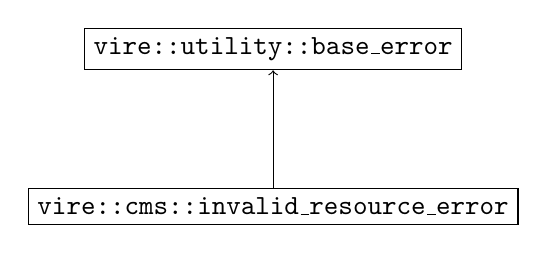
\begin{tikzpicture}
  \node (base)  at (0,2)  [draw] {\texttt{vire::utility::base\_error}};
  \node (ire)  at (0,0) [draw] {\texttt{vire::cms::invalid\_resource\_error}};
  \draw[->] (node cs:name=ire,anchor=north)
  |- (0,1) -| (node cs:name=base,anchor=south);
\end{tikzpicture}
\end{center}

\begin{figure}[h]
\vskip 10pt
\small
\begin{Verbatim}[frame=single,xleftmargin=0.cm,label=\fbox{C++}]
struct vire::cms::invalid_resource_error : public vire::utility::base_error
{
  // Attributes:
  std::string invalid_resource_path; // Invalid resource path
  std::string invalid_resource_id;   // Invalid resource internal ID (Vire server only)
};
\end{Verbatim}
\normalsize
\caption{The structure  of a invalid resource error object (C++).}
\label{fig-app-payload-invalid_resource_error}
\end{figure}

\begin{figure}[h]
\vskip 10pt
\small
\begin{Verbatim}[frame=single,xleftmargin=0.cm,label=\fbox{JSON++}]
{
  "code" : "3",
  "message_format" : "Resource path 'Atlas://Calorimeter/HV/Crate1/stop' is invalid",
  "invalid_resource_path" : "Atlas://Calorimeter/HV/Crate1/stop"
}
\end{Verbatim}
\normalsize
\caption{JSON formatted invalid resource error object.}
\label{fig-app-payload-invalid_resource_error-json}
\end{figure}


\item
Class     \texttt{vire::cms::resource\_status\_record}    (figure
\ref{fig-app-payload-resource_status_record}).

\end{itemize}

\begin{figure}[h]
\vskip 10pt
\small
\begin{Verbatim}[frame=single,xleftmargin=0.cm,label=\fbox{C++}]
struct vire::cms::resource_status_record
{
  // Attributes:
  std::string path;      // Path of the resource
  std::string timestamp; // Timestamp of the last modification
  uint16_t    flags;     // Status bits (Missing/Disabled/Pending/Error)
};
\end{Verbatim}
\normalsize
\caption{The structure  of a resource status record object (C++).}
\label{fig-app-payload-resource_status_record}
\end{figure}


\begin{figure}[h]
\vskip 10pt
\small
\begin{Verbatim}[frame=single,xleftmargin=0.cm,label=\fbox{JSON}]
{
  "path" : "SuperNEMO://Demonstrator/CMS/Coil/Control/Current/__dp_read__",
  "timestamp" : "20160612T212432.324517",
  "flags" : 2
}
\end{Verbatim}
\normalsize
\caption{JSON formatted resource status record object.}
\label{fig-app-payload-resource_status_record-json}
\end{figure}

\vfill
\pagebreak
\clearpage

\subsection{Connection of the Vire server to the CMS server}


\begin{itemize}

\item   The   \texttt{vire::cmslapp::connection\_request}   class
  (version \texttt{1.0})  represents a connection request  sent by the
  Vire server to the  CMS server through the \textcolor{blue}{service}
  channel.

\begin{center}
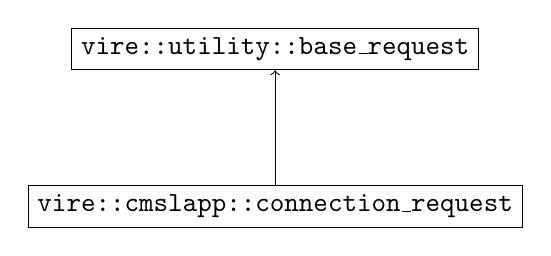
\begin{tikzpicture}
  \node (base)  at (0,2)  [draw] {\texttt{vire::utility::base\_request}};
  \node (cr)  at (0,0) [draw] {\texttt{vire::cmslapp::connection\_request}};
  \draw[->] (node cs:name=cr,anchor=north)
  |- (0,1) -| (node cs:name=base,anchor=south);
\end{tikzpicture}
\end{center}

\noindent Class registration:
\begin{itemize}
\item name: \texttt{"vire::cmslapp::connection\_request"}
\item version: "1.0"
\end{itemize}

\begin{figure}[h]
\vskip 10pt
\small
\begin{Verbatim}[frame=single,xleftmargin=0.cm,label=\fbox{C++}]
struct vire::cmslapp::connection_request : public vire::utility::base_request
{
  // Attributes:
  vire::utility::instance_identifier  setup_id; // Identifier of the experimental setup
  std::vector<std::string> requested_resources; // The list of requested resources
                                                // addressed by path
};
\end{Verbatim}
\normalsize
\caption{The structure of the connection  request object to be emitted
  by the Vire server to the CMS server (C++).}
\label{fig-app-payload-connection_request}
\end{figure}

\begin{figure}[h]
\vskip 10pt
\small
\begin{Verbatim}[frame=single,xleftmargin=0.cm,label=\fbox{JSON}]
{
  "setup_id" : {
    "name" : "snemo",
    "version" : "1.0.2"
  },
  "requested_resources" : [
    "SuperNEMO://Demonstrator/CMS/Coil/PS/Control/Current/__dp_read__",
    "SuperNEMO://Demonstrator/CMS/Coil/PS/Control/Current/__dp_write__",
    ...
    "SuperNEMO://Demonstrator/CMS/Acquisition/start",
    "SuperNEMO://Demonstrator/CMS/Acquisition/stop"
  ]
}
\end{Verbatim}
\normalsize
\caption{A JSON formatted  connection request object sent  by the Vire
  server to the CMS server (C++).}
\label{fig-app-payload-connection_request-json}
\end{figure}


\item  The  \texttt{vire::cmslapp::connection\_success\_response}
  class represents  the response sent back  to the Vire server  by the
  CMS server through the  \textcolor{blue}{service} channel in case of
  success.

\begin{center}
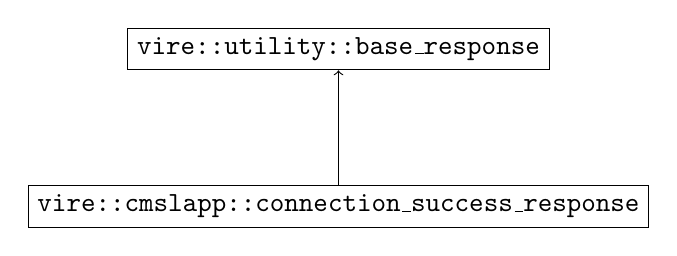
\begin{tikzpicture}
  \node (base)  at (0,2)  [draw] {\texttt{vire::utility::base\_response}};
  \node (csr)  at (0,0) [draw] {\texttt{vire::cmslapp::connection\_success\_response}};
  \draw[->] (node cs:name=csr,anchor=north)
  |- (0,1) -| (node cs:name=base,anchor=south);
\end{tikzpicture}
\end{center}

\noindent Class registration:
\begin{itemize}
\item name: \texttt{"vire::cmslapp::connection\_success\_response"}
\item version: "1.0"
\end{itemize}

\begin{figure}[h]
\vskip 10pt
\small
\begin{Verbatim}[frame=single,xleftmargin=0.cm,label=\fbox{C++}]
struct connection_success_response
  : public vire::utility::base_response
{
  typedef vire::resource::resource_status_record resource_status_record; // Type alias

  // Attributes:
  std::vector<resource_status_record> resources_snapshot; // Requested resources snapshot
};
\end{Verbatim}
\normalsize
\caption{The structure  of the connection success  response emitted by
  the CMS server to the Vire server (C++).}
\label{fig-app-payload-connection_success_response}
\end{figure}



\begin{figure}[h]
\vskip 10pt
\small
\begin{Verbatim}[frame=single,xleftmargin=0.cm,label=\fbox{\texttt{JSON}}]
{
  "resources_snapshot"  : [
    {
      "path" : "SuperNEMO://Demonstrator/CMS/Coil/PS/Control/Current/__dp_read__",
      "timestamp" : "20160612T212432.324517",
      "flags" : "0000"
    },
    {
      "path" : "SuperNEMO://Demonstrator/CMS/Coil/PS/Control/Current/__dp_write__",
      "timestamp" : "20160612T212432.328732",
      "flags" : "0000"
    },
    ...
    {
      "path" : "SuperNEMO://Demonstrator/CMS/Acquisition/start",
      "timestamp" : "20160612T212432.371671",
      "flags" : "0000"
    },
    {
      "path" : "SuperNEMO://Demonstrator/CMS/Acquisition/stop",
      "timestamp" : "20160612T212432.373624",
      "flags" : "0100"
    }
  ]
}
\end{Verbatim}
\normalsize
\caption[JSON formatted  connection success response]  {JSON formatted
  connection        success        response       object        (class
  \texttt{vire::cmslapp::connection\_success\_response}.}
\label{fig-app-payload-connection_success_response-json}
\end{figure}


\item
The  \texttt{vire::cmslapp::connection\_failure\_response}  class
represents the response sent back to the Vire server by the CMS server
through the \textcolor{blue}{service} channel in case of failure.

\begin{center}
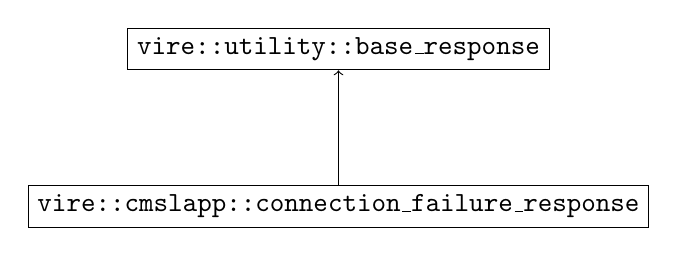
\begin{tikzpicture}
  \node (base)  at (0,2)  [draw] {\texttt{vire::utility::base\_response}};
  \node (cfr)  at (0,0) [draw] {\texttt{vire::cmslapp::connection\_failure\_response}};
  \draw[->] (node cs:name=cfr,anchor=north)
  |- (0,1) -| (node cs:name=base,anchor=south);
\end{tikzpicture}
\end{center}

\begin{figure}[h]
\vskip 10pt
\small
\begin{Verbatim}[frame=single,xleftmargin=0.cm,label=\fbox{C++}]
struct connection_failure_response
  : public vire::utility::base_response
{
  // Nested type alias:
  typedef vire::utility::model_identifier error_identifier;

  // Nested error type aliases:
  typedef vire::utility::invalid_context_error invalid_context_error;
  typedef vire::utility::invalid_setup_id_error invalid_setup_id_error;

  // Nested error type:
  struct unknown_resources_error : public vire::utility::base_error {
    std::vector<std::string> unknown_paths; // List of unknown resources' paths
  };

  // Attributes:
  error_identifier error_id; // Error type identifier
  XXX_error        error;    // Embedded error record of one of the nested error type above
};
\end{Verbatim}
\normalsize
\caption{The structure  of the  connection failure response emitted
  by the CMS server to the Vire server (C++).}
\label{fig-app-payload-connection_failure_response}
\end{figure}


\end{itemize}

% \texttt{vire::cmsserver::disconnection\_request} (version \texttt{1.0})

\vfill
\pagebreak
\clearpage


\subsection{Disconnection of the Vire server from the CMS server}

\begin{itemize}

\item  The  \texttt{vire::cmslapp::disconnection\_request}  class
  represents a  disconnection request sent  by the Vire server  to the
  CMS server through the \textcolor{blue}{service} channel.

\begin{center}
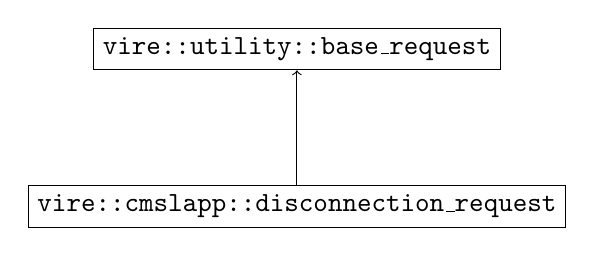
\begin{tikzpicture}
  \node (base)  at (0,2)  [draw] {\texttt{vire::utility::base\_request}};
  \node (cr)  at (0,0) [draw] {\texttt{vire::cmslapp::disconnection\_request}};
  \draw[->] (node cs:name=cr,anchor=north)
  |- (0,1) -| (node cs:name=base,anchor=south);
\end{tikzpicture}
\end{center}

\noindent Class registration:
\begin{itemize}
\item name: \texttt{"vire::cmslapp::disconnection\_request"}
\item version: "1.0"
\end{itemize}

\begin{figure}[h]
\vskip 10pt
\small
\begin{Verbatim}[frame=single,xleftmargin=0.cm,label=\fbox{C++}]
struct disconnection_request : public vire::utility::base_request {
};
\end{Verbatim}
\normalsize
\caption{The structure of the disconnection  request object to be emitted
  by the Vire server to the CMS server (C++).}
\label{fig-app-payload-disconnection_request}
\end{figure}

%% \begin{figure}[h]
%% \vskip 10pt
%% \small
%% \begin{Verbatim}[frame=single,xleftmargin=0.cm,label=\fbox{C++}]
%% {
%% }
%% \end{Verbatim}
%% \normalsize
%% \caption{A JSON formatted  connection request object sent  by the Vire
%%   server to the CMS server (C++).}
%% \label{fig-app-payload-connection_request-json}
%% \end{figure}


\item  The  \texttt{vire::cmslapp::disconnection\_success\_response}
  class represents  the response sent back  to the Vire server  by the
  CMS server through the  \textcolor{blue}{service} channel in case of
  success.

\begin{center}
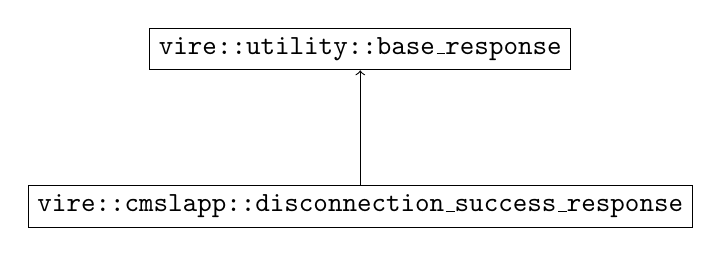
\begin{tikzpicture}
  \node (base)  at (0,2)  [draw] {\texttt{vire::utility::base\_response}};
  \node (csr)  at (0,0) [draw] {\texttt{vire::cmslapp::disconnection\_success\_response}};
  \draw[->] (node cs:name=csr,anchor=north)
  |- (0,1) -| (node cs:name=base,anchor=south);
\end{tikzpicture}
\end{center}


\noindent Class registration:
\begin{itemize}
\item name: \texttt{"vire::cmslapp::disconnection\_success\_response"}
\item version: "1.0"
\end{itemize}

\begin{figure}[h]
\vskip 10pt
\small
\begin{Verbatim}[frame=single,xleftmargin=0.cm,label=\fbox{C++}]
struct disconnection_success_response
  : public vire::utility::base_response
{
};
\end{Verbatim}
\normalsize
\caption{The structure  of the disconnection success  response emitted by
  the CMS server to the Vire server (C++).}
\label{fig-app-payload-disconnection_success_response}
\end{figure}


\end{itemize}


\vfill
\pagebreak
\clearpage

\subsection{Resource related payload objects}

\subsubsection{Resource Pub/Sub service}

\begin{itemize}

\item  The \texttt{vire::resource::resource\_pubsub\_request} object is responsible of
  demanding the activation/deactivation of the Pub/Sub service associated to a given
  resource (fig. \ref{fig-app-payload-resource_pubsub_request}).

\begin{figure}[h]
\vskip 10pt
\small
\begin{Verbatim}[frame=single,xleftmargin=0.cm,label=\fbox{C++}]
struct resource_pubsub_request
  : public vire::utility::base_request
{
  // Attributes:
  std::string path;      // The resource path.
  bool        subscribe; // Pub/Sub service (un)subscribe flag.
};
\end{Verbatim}
\normalsize
\caption{The structure of the \texttt{vire::resource::resource\_pubsub\_request}
  class (C++).}
\label{fig-app-payload-resource_pubsub_request}
\end{figure}

\item The \texttt{vire::resource::resource\_pubsub\_success\_response}
  object encapsulate a  successfull response of the CMS  server to the
  Vire  server  concerning   the  subscription/unsubscription  of  the
  Pub/Sub     service    associated     to     a    given     resource
  (fig. \ref{fig-app-payload-resource_pubsub_success_response}).

\begin{figure}[h]
\vskip 10pt
\small
\begin{Verbatim}[frame=single,xleftmargin=0.cm,label=\fbox{C++}]
struct resource_pubsub_success_response
  : public vire::utility::base_response
{
  // Pub/Sub mechanism type alias:
  typedef vire::resource::amqp_mechanism_address amqp_mechanism_address;

  // Type alias:
  typedef vire::utility::model_identifier pubsub_mechanism_identifier;
  typedef boost::variant<
      amqp_mechanism_address
      > pubsub_address_type;

  // Attributes:
  std::string                 path;               // The resource path.
  bool                        subscribe;          // The effective (un)subscribe flag.
  pubsub_mechanism_identifier pubsub_mechanism_id; // The mechanism for accessing Pub/Sub service
  pubsub_address_type         pubsub_address;      // If activation is set, this describes the
                                                   // access to the Pub/Sub service.
};
\end{Verbatim}
\normalsize
\caption{The structure of the \texttt{vire::resource::resource\_pubsub\_success\_response}
  class (C++).}
\label{fig-app-payload-resource_pubsub_success_response}
\end{figure}

\small
\begin{Verbatim}[frame=single,xleftmargin=0.cm,label=\fbox{JSON++}]
{
  "path" : "SuperNEMO://Demonstrator/CMS/Coil/PS/Monitoring/__dp_read__",
  "subscribe" : "true",
  "pubsub_mechanism_id" : "vire::amqp",
  "pubsub_address" : {
     "server" : "snemo.amqp",
     "port" : 1234,
     "channel" : "snemo.amqp.cms.pubsub.WAqq7ERzs1",
     "binding" : "SuperNEMO://Demonstrator/CMS/Coil/PS/Monitoring/__dp_read__",
     "key" : "coil.monitoring.pubsub"
  }
}
\end{Verbatim}
\normalsize

\item    The   \texttt{vire::resource::amqp\_mechanism\_address}    object
  describes   the  access   to   Pub/Sub   service  through   RabbitMQ
  (fig. \ref{fig-app-payload-amqp_pubsub_access_type}).

\begin{figure}[h]
\vskip 10pt
\small
\begin{Verbatim}[frame=single,xleftmargin=0.cm,label=\fbox{C++}]
struct amqp_mechanism_address
{
  // Attributes:
  std::string server;  // The AMQP server
  int         port;    // The AMQP server port
  std::string channel; // The RabbitMQ Pub/Sub channel.
  std::string binding; // The binding dedicated to this Pub/Sub service.
  std::string key;     // The Pub/Sub specific key/topic.
};
\end{Verbatim}
\normalsize
\caption{The structure of the \texttt{vire::resource::amqp\_pubsub\_access\_type}
  class (C++).}
\label{fig-app-payload-amqp_pubsub_access_type}
\end{figure}


\item The \texttt{vire::resource::resource\_pubsub\_failure\_response}
  object describes a failure response  concerning a request on Pub/Sub
  service       associated       to       a       given       resource
  (fig. \ref{fig-app-payload-resource_pubsub_failure_response}).


\begin{figure}[h]
\vskip 10pt
\small
\begin{Verbatim}[frame=single,xleftmargin=0.cm,label=\fbox{C++}]
struct resource_pubsub_failure_response
  : public vire::utility::base_response
{
  // Nested type alias:
  typedef vire::utility::model_identifier error_type_identifier;

  // Nested error type aliases:
  typedef vire::utility::invalid_context_error  invalid_context_error;
  typedef vire::utility::invalid_resource_error invalid_resource_error;

  // Nested error type:
  struct no_pubsub_resource_error : public vire::utility::base_error {
    std::string path; // The path of the resource without Pub/Sub service support
  };

  typedef boost::variant<
     invalid_context_error,
     invalid_resource_error,
     no_pubsub_resource_error
     > error_type;

  // Attributes:
  error_type_identifier error_type_id; // Error type identifier.
  error_type            error;        // Embedded error record of one of
                                      // the nested error types above.
};
\end{Verbatim}
\normalsize
\caption{The structure of the \texttt{vire::resource::resource\_pubsub\_failure\_response}
  class (C++).}
\label{fig-app-payload-resource_pubsub_failure_response}
\end{figure}

\end{itemize}

\vfill
\pagebreak
\clearpage

\subsubsection{Fetching resource status}

\begin{center}
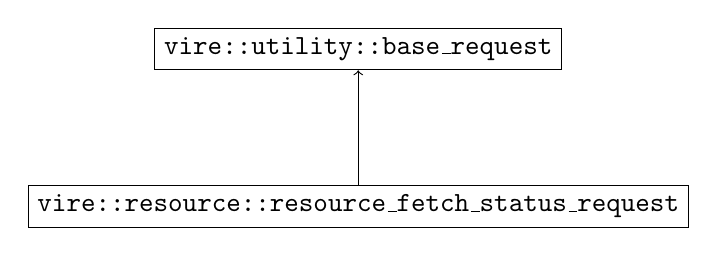
\begin{tikzpicture}
  \node (payload)  at (0,2) [draw] {\texttt{vire::utility::base\_request}};
  \node (request)  at (0,0) [draw] {\texttt{vire::resource::resource\_fetch\_status\_request}};
  \draw[->] (node cs:name=request,anchor=north)
  |- (0,1) -| (node cs:name=payload,anchor=south);
\end{tikzpicture}
\end{center}

\begin{itemize}

\item The \texttt{vire::resource::resource\_fetch\_status\_request} object
  demands to the CMS server an updated status record associated to a given resource
(fig. \ref{fig-app-payload-resource_fetch_status_request}).

\begin{figure}[h]
\vskip 10pt
\small
\begin{Verbatim}[frame=single,xleftmargin=0.cm,label=\fbox{C++}]
struct resource_fetch_status_request
  : public vire::utility::base_request
{
  // Attributes:
  std::string path; // Resource path.
};
\end{Verbatim}
\normalsize
\caption{The structure of a \texttt{vire::utility::resource\_fetch\_status\_request} object
  (C++).}
\label{fig-app-payload-resource_fetch_status_request}
\end{figure}

\item The \texttt{vire::resource::resource\_fetch\_status\_success\_response} object
  transmits the updated/current status record  associated to a given resource
(fig. \ref{fig-app-payload-resource_fetch_status_success_response}).

\begin{figure}[h]
\vskip 10pt
\small
\begin{Verbatim}[frame=single,xleftmargin=0.cm,label=\fbox{C++}]
struct resource_fetch_status_success_response
  : public vire::utility::base_response
{
  // Nested type alias:
  typedef vire::resource::resource_status_record resource_status_record;

  // Attributes:
  resource_status_record status; // The resource status record.
};
\end{Verbatim}
\normalsize
\caption{The structure of a \texttt{vire::utility::resource\_fetch\_status\_success\_response} object
  (C++).}
\label{fig-app-payload-resource_fetch_status_success_response}
\end{figure}



\item The \texttt{vire::resource::resource\_fetch\_status\_failure\_response} object
  describes a failure detected by the CMS server in response to a resource fetch status request.

\begin{figure}[h]
\vskip 10pt
\small
\begin{Verbatim}[frame=single,xleftmargin=0.cm,label=\fbox{C++}]
struct resource_fetch_status_failure_response
  : public vire::utility::base_response
{
  // Nested type alias:
  typedef vire::utility::model_identifier error_identifier;

  // Nested error type aliases:
  typedef vire::utility::invalid_context_error   invalid_context_error;
  typedef vire::resource::invalid_resource_error invalid_resource_error;

  // Attributes:
  error_identifier error_id; // Error type identifier
  XXX_error        error;    // Embedded error record of one of the nested error type above
};
\end{Verbatim}
\normalsize
\caption{The structure of a \texttt{vire::utility::resource\_fetch\_status\_failure\_response} object
  (C++).}
\label{fig-app-payload-resource_fetch_status_failure_response}
\end{figure}


\end{itemize}


\vfill
\pagebreak
\clearpage

\subsubsection{Synchronous/blocking resource execution}

\begin{center}
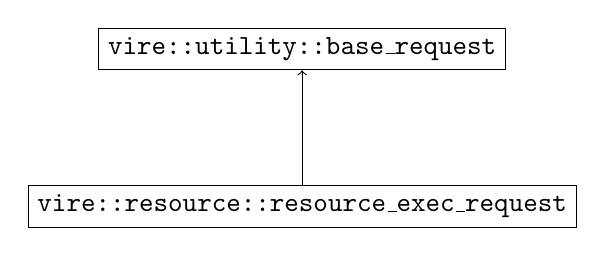
\begin{tikzpicture}
  \node (payload)  at (0,2)   [draw] {\texttt{vire::utility::base\_request}};
  \node (request)  at (0,0)  [draw] {\texttt{vire::resource::resource\_exec\_request}};
  \draw[->] (node cs:name=request,anchor=north)
  |- (0,1) -| (node cs:name=payload,anchor=south);
\end{tikzpicture}
\end{center}

\begin{itemize}

\item The \texttt{vire::resource::resource\_exec\_request} object represent a resource execution request
in blocking (synchronous) mode.


\begin{figure}[h]
\vskip 10pt
\small
\begin{Verbatim}[frame=single,xleftmargin=0.cm,label=\fbox{C++}]
struct resource_exec_request
  : public vire::utility::base_request
{
  // Type alias:
  typedef vire::resource::method_argument method_argument;

  // Attributes:
  std::string                  path;            // Resource path.
  std::vector<method_argument> input_arguments; // Embedded error record of one of
                                                // the nested error type above.
};
\end{Verbatim}
\normalsize
\caption{The structure of a \texttt{vire::utility::resource\_fetch\_status\_failure\_response} object
  (C++).}
\label{fig-app-payload-resource_fetch_status_failure_response}
\end{figure}

\item \texttt{vire::resource::resource\_exec\_success\_response}

\small
\begin{Verbatim}[frame=single,xleftmargin=0.cm,label=\fbox{C++}]
struct resource_exec_success_response
 : vire::utility::base_response
{
  // Type alias:
  typedef vire::resource::method_argument        method_argument;
  typedef vire::resource::resource_status_record resource_status_record;

  // Attributes:
  resource_status_record       status;               // Resource status
  std::string                  reception_timestamp;  // Request reception timestamp
  std::string                  completion_timestamp; // Execution completion timestamp
  std::vector<method_argument> output_arguments;     // Output arguments
};
\end{Verbatim}



\item \texttt{vire::resource::resource\_exec\_failure\_response}


\small
\begin{Verbatim}[frame=single,xleftmargin=0.cm,label=\fbox{C++}]
struct resource_exec_failure_response
 : vire::utility::base_response
{

  // Error type aliases:
  typedef vire::utility::invalid_context_error   invalid_context_error;
  typedef vire::resource::invalid_resource_error invalid_resource_error;
  typedef vire::resource::invalid_status_error   invalid_status_error;
  typedef vire::resource::resource_exec_error    resource_exec_error;

  // Type aliases:
  typedef vire::utility::model_identifier        error_type_identifier;
  typedef boost::variant<
      invalid_context_error,
      invalid_resource_error,
      invalid_status_error,
      resource_exec_error> error_type;

  // Attributes:
  error_type_identifier error_type_id; // Error type identifier
  error_type            error;        // Embedded error record

};
\end{Verbatim}

\end{itemize}


\vfill
\pagebreak
\clearpage

\subsubsection{Asynchronous/non-blocking resource execution}

\begin{center}
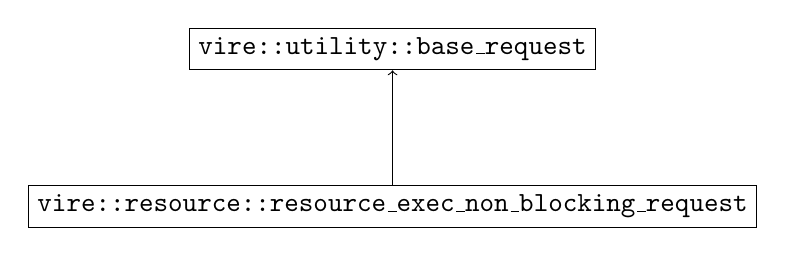
\begin{tikzpicture}
  \node (payload)  at (0,2)   [draw] {\texttt{vire::utility::base\_request}};
  \node (request_nb)  at (0,0)  [draw] {\texttt{vire::resource::resource\_exec\_non\_blocking\_request}};
  \draw[->] (node cs:name=request_nb,anchor=north)
  |- (0,1) -| (node cs:name=payload,anchor=south);
\end{tikzpicture}
\end{center}

\begin{itemize}

\item \texttt{vire::resource::resource\_exec\_non\_blocking\_request}
\small
\begin{Verbatim}[frame=single,xleftmargin=0.cm,label=\fbox{C++}]
struct resource_exec_non_blocking_request
  : public vire::utility::base_request
{
  // Type alias:
  typedef vire::resource::method_argument method_argument;

  // Attributes:
  std::string                  path;            // Resource path.
  std::vector<method_argument> input_arguments; // Embedded error record of one of
                                                // the nested error type above.

};
\end{Verbatim}

\item \texttt{vire::resource::resource\_exec\_non\_blocking\_ack\_response}


\small
\begin{Verbatim}[frame=single,xleftmargin=0.cm,label=\fbox{C++}]
struct resource_exec_non_blocking_ack_response
 : vire::utility::base_response
{
  // Type alias:
  typedef vire::resource::method_argument        method_argument;
  typedef vire::resource::resource_status_record resource_status_record;

  // Attributes:
  resource_status_record       status;
  std::string                  reception_timestamp;

};
\end{Verbatim}


\item \texttt{vire::resource::resource\_exec\_non\_blocking\_noack\_response}


\small
\begin{Verbatim}[frame=single,xleftmargin=0.cm,label=\fbox{C++}]
struct resource_exec_non_blocking_noack_response
  : vire::utility::base_response
{
  // Type alias:
  typedef vire::resource::resource_status_record resource_status_record;
  typedef vire::utility::model_identifier error_type_identifier;

  // Error type aliases:
  typedef vire::utility::invalid_context_error   invalid_context_error;
  typedef vire::resource::invalid_resource_error invalid_resource_error;
  typedef vire::resource::invalid_status_error   invalid_status_error;
  typedef vire::resource::resource_exec_error    resource_exec_error;

  // Nested error type:
  struct no_non_blocking_exec_resource_error : public vire::utility::base_error {
    std::string path; // The path of the resource without non-blocking execution support
  };

  typedef boost::variant<
     invalid_context_error,
     invalid_resource_error,
     invalid_status_error,
     no_non_blocking_exec_resource_error,
     resource_exec_error
     > error_type;

  // Attributes:
  resource_status_record status;        // Resource status.
  error_type_identifier  error_type_id; // Error type identifier.
  error_type             error;         // Embedded error record of one of
                                        // the nested error types above.

};
\end{Verbatim}
\normalsize


\item \texttt{vire::resource::resource\_exec\_non\_blocking\_success\_event}


\small
\begin{Verbatim}[frame=single,xleftmargin=0.cm,label=\fbox{C++}]
struct resource_exec_non_blocking_success\_event
  : vire::utility::base_event
{
  // Type alias:
  typedef vire::resource::method_argument        method_argument;
  typedef vire::resource::resource_status_record resource_status_record;

  // Attributes:
  resource_status_record       status;               // Resource status
  std::string                  reception_timestamp;  // Request reception timestamp
  std::string                  completion_timestamp; // Execution completion timestamp
  std::vector<method_argument> output_arguments;     // Output arguments

};
\end{Verbatim}
\normalsize

\item \texttt{vire::resource::resource\_exec\_non\_blocking\_failure\_event}


\small
\begin{Verbatim}[frame=single,xleftmargin=0.cm,label=\fbox{C++}]
struct resource_exec_non_blocking_failure\_event
  : vire::utility::base_event
{

  // Error type aliases:
  typedef vire::utility::invalid_context_error   invalid_context_error;
  typedef vire::cms::invalid_resource_error invalid_resource_error;
  typedef vire::cms::invalid_status_error   invalid_status_error;
  typedef vire::cms::resource_exec_error    resource_exec_error;

  // Type aliases:
  typedef vire::utility::model_identifier        error_type_identifier;
  typedef boost::variant<
      vire::utility::invalid_context_error,
      vire::cms::invalid_resource_error,
      vire::cms::invalid_status_error,
      vire::cms::resource_exec_error> error_type;

  // Attributes:
  error_type_identifier error_type_id; // Error type identifier
  error_type            error;        // Embedded error record

};
\end{Verbatim}
\normalsize


\end{itemize}


\vfill
\pagebreak
\clearpage

% end


\section{The RabbitMQ based RPC system}\label{app:rabbitmq_rpc}

\subsection{Introduction}


\end{document}
%%

\section{Interaction of the CMS/LAPP server with Vire clients}

TODO
\vfill
\pagebreak
\clearpage

%%%%%%%%%
\appendix


\section{Filesystem and configuration files management}\label{app:filesystem_conf}

Let's consider  a simple  situation where  one runs  the Vire  and CMS
software  tools (servers)  on a  single Linux  machine (the  CMS host)
under            the            \texttt{"nemoprod"}            generic
account\footnote{\texttt{"nemoprod"}  is  the   login  of  th  generic
  account used at the CCIN2P3  cluster to perform automated management
  operations on experimental and  Monte-Carlo data file: data transfer
  from LSM or LSC labs to CCIN2P3, calibration and reconstruction data
  processing, storage on HPPS.}.

\begin{itemize}
\item Hostname login : \verb|192.168.1.10| (private IP) %\texttt{snemocms.lsm.in2p3.fr} (public address)
\item User login : \texttt{nemoprod}
\item Main group : \texttt{supernemo}
\item Home directory : \verb|/home/nemoprod| (a.k.a. \verb|~nemoprod|)
\end{itemize}

\noindent  We  assume that  the  SuperNEMO  online software  has  been
installed   and  setup   in  the   home  directory,   for  example in
\verb|/home/nemoprod/Private/Software/| :
\vskip 20pt
\small
\begin{Verbatim}[frame=single,xleftmargin=0.cm,label=\fbox{Filesystem}]
/home/nemoprod/Private/Software
|-- Cadfael/ # base directory of the Cadfael software framework
|-- Bayeux/  # base directory of the Bayeux software framework
|-- Vire/    # base directory of the Vire software framework
|-- OPCUA/   # base directory of the OPCUA+MOS software framework
`-- Falaise/ # base directory of the Falaise software framework
\end{Verbatim}
\normalsize

\noindent  We consider  here  that the  Falaise  library package  will
contain  the mandatory  configuration files  that describe  the online
software, both for the Vire and CMS/MOS parts:
\vskip 20pt
\small
\begin{Verbatim}[frame=single,xleftmargin=0.cm,label=\fbox{Filesystem}]
/home/nemoprod/Private/Software
:
`-- Falaise/
    :
    `-- Install/
        `-- Falaise-3.0.0/
            |-- bin/
            |   :
            |   |-- flquery
            |   |-- flreconstruct
            |   `-- flsimulate
            |-- include/
            :   :
            |-- lib/
            |   `-- x86_64-linux-gnu/
            |       :
            |       |-- libFalaise.so
            |       :
            `-- share/
                `-- Falaise-3.0.0/
                    `-- resources/
                        `-- config/
                            `-- online/
                                :
                                :
\end{Verbatim}
\normalsize

\noindent Where:
\begin{itemize}
\item                                                              the
  \verb|/home/nemoprod/Private/Software/Falaise/Install/Falaise-3.0.0|
  is  the  installation  prefix  of  the  Falaise  library  (binaries,
  includes) and associated resource files.
\item      the     \verb|share/Falaise-3.0.0/resources/config/online/|
  subdirectory  is the  tree  of configuration  files  that should  be
  accessible  by  any online  software  component  (Vire server,  Vire
  clients, CMS and MOS servers).
\end{itemize}


\noindent  Let's consider  the \verb|.../config/online/|  directory as
the base directory for all online configuration files for the Vire and
CMS  servers.   All  configuration  files  should  thus  be  addressed
relatively to this place.

\noindent  We  propose to  use  one  of  the following  techniques  to
represent this base directory:

\begin{itemize}
\item         a         dedicated         environment         variable
  \verb|SNEMO_ONLINE_CONFIG_BASE_DIR| recognized by  both Vire and CMS
  servers. It could be setup within the environment with:
\vskip 20pt
\small
\begin{Verbatim}[frame=single,xleftmargin=0.cm,label=\fbox{shell}]
export FALAISE_INSTALL_DIR=\
  ${HOME}/Private/Software/Falaise/Install/Falaise-3.0.0
export SNEMO_ONLINE_CONFIG_BASE_DIR=\
  ${FALAISE_INSTALL_DIR}/share/Falaise-3.0.0/resources/config/online
\end{Verbatim}
\normalsize

\item a  path registration label as  implemented in the kernel  of the
  Bayeux library:\\
  \noindent The \verb|@snonlinecfg:| label \\
  is associated to\\
  \noindent \hskip 50pt\verb|${FALAISE_INSTALL_DIR}/share/Falaise-3.0.0/resources/config/online|

\end{itemize}

\noindent Thus a specific  configuration file \verb|dummy.conf| could be
addressed with one of the following syntaxes:

\begin{itemize}

\item[(a)]
  \verb|${SNEMO_ONLINE_CONFIG_BASE_DIR}/snemo/1.0.2/dummy.conf|       :
  supported  by  Vire  and  CMS  using  word  expansion  utility  like
  \texttt{wordexp} (for C/C++ languages),

\item[(b)]  \verb|@snonlinecfg:snemo/1.0.2/dummy.conf|  : supported  by
  Vire  only  for  now,  thanks to  the  path  registration  mechanism
  implemented in the Bayeux API,

\item[(c)] \verb|snemo/1.0.2/dummy.conf| : can be supported by Vire and
  CMS  but  is  ambiguous  because  such a relative  path  can  be  also
  interpreted as a path relatively  to the current directory (\verb|./|)
  and not to the online configuration directory.

\end{itemize}

We suggests  the use  of an  explicit environment  variable as  in (a)
because it  is simple to  implement in various languages  and software
frameworks and should not imply any ambiguous file path resolution.

\vfill
\pagebreak
\clearpage

% end


\section{Integration of a new device}\label{app:new_device}

Both Vire  and MOS systems are  designed to be expandable  in terms of
device integration.  This section  decribes the  integration of  a new
device in the \emph{Control and Monitoring System}.

\subsection{Integration of a new device in the MOS environment}

Any new device is described through  a dedicated XML model file.  This
XML  file  is  created  from  a  template  file  elaborated  from  the
\emph{interface control document} (ICD) and associated to the model of
the  device. The  format  of the  XML  file is  described  in the  MOS
(Multipurpose OPCUA Server) User Guide. % ref

Typically, a device is embedded in a OPCUA server and implemented as a
OPCUA  \emph{simple  device}.   The  OPCUA server  itself  is  located
through an unique dedicated IP address and port.

The simple device  instance, hosted in the OPCUA  server, may contains
other sub-devices and/or \emph{datapoints}.   It is thus considered as
the root  of a hierarchy  of daughter  objects at deeper  levels.  The
daughter objects (devices or datapoints) are named relatively to their
top level  parent device. Figure  \ref{fig:an:mos_dev_1} shows an
example of a device embedded in a MOS server.

\begin{figure}[h]
\begin{center}
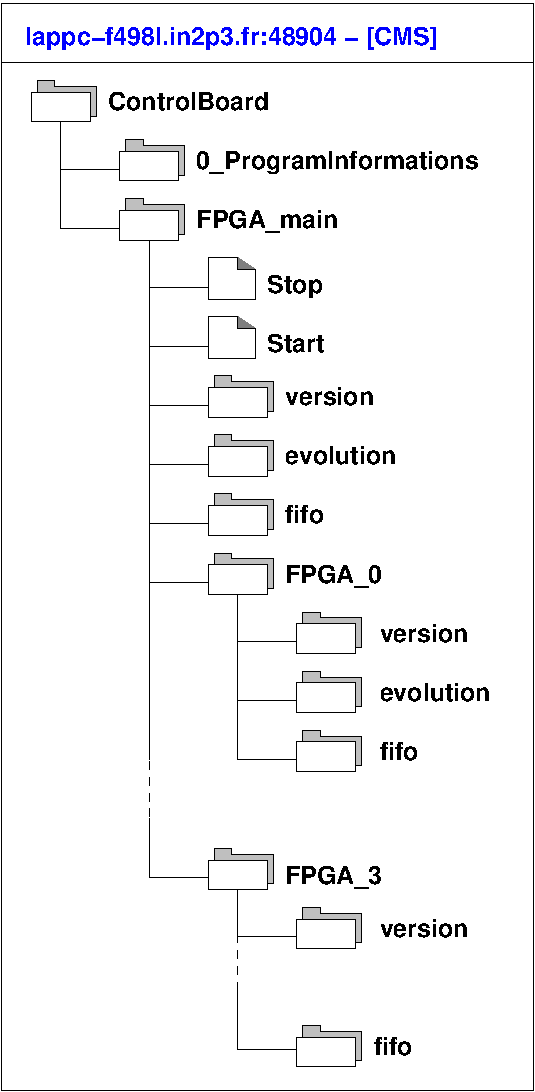
\includegraphics[width=5cm]{appendix/images/MOS_device_example_1.pdf}
\end{center}
\caption{Example of a  device managed through a MOS  server.  The root
  device is named \texttt{ControlBoard}.  First level daughter devices
  are  \texttt{0\_ProgramInformations} and  \texttt{FPGA\_main}.  Here
  the          MOS/OPCUA          server          is          labelled
  \texttt{CMS}.}\label{fig:an:mos_dev_1}
\end{figure}

% TODO


\subsection{Integration of a new device in the Vire environment}

The Vire  API also implements a  mechanism to describe a  hierarchy of
devices.  This  mechanism is independant  of the  one used in  the MOS
system but can  be easily made compatible with it.   This means that a
MOS  hierarchy  of devices  can  be  represented  in Vire.   The  Vire
hierarchy of  devices can  be considered as  some kind  of filesystem,
each device  being a folder with  its unique path, as  shown on figure
\ref{fig:an:mos_dev_2}.   The \emph{methods}  associated to  a devices
(or a datapoint) can be considered as plain executable files stored in
the  device's folder  : they  constitute the  set of  \emph{resources}
associated to the device.


\begin{figure}[h]
\begin{center}
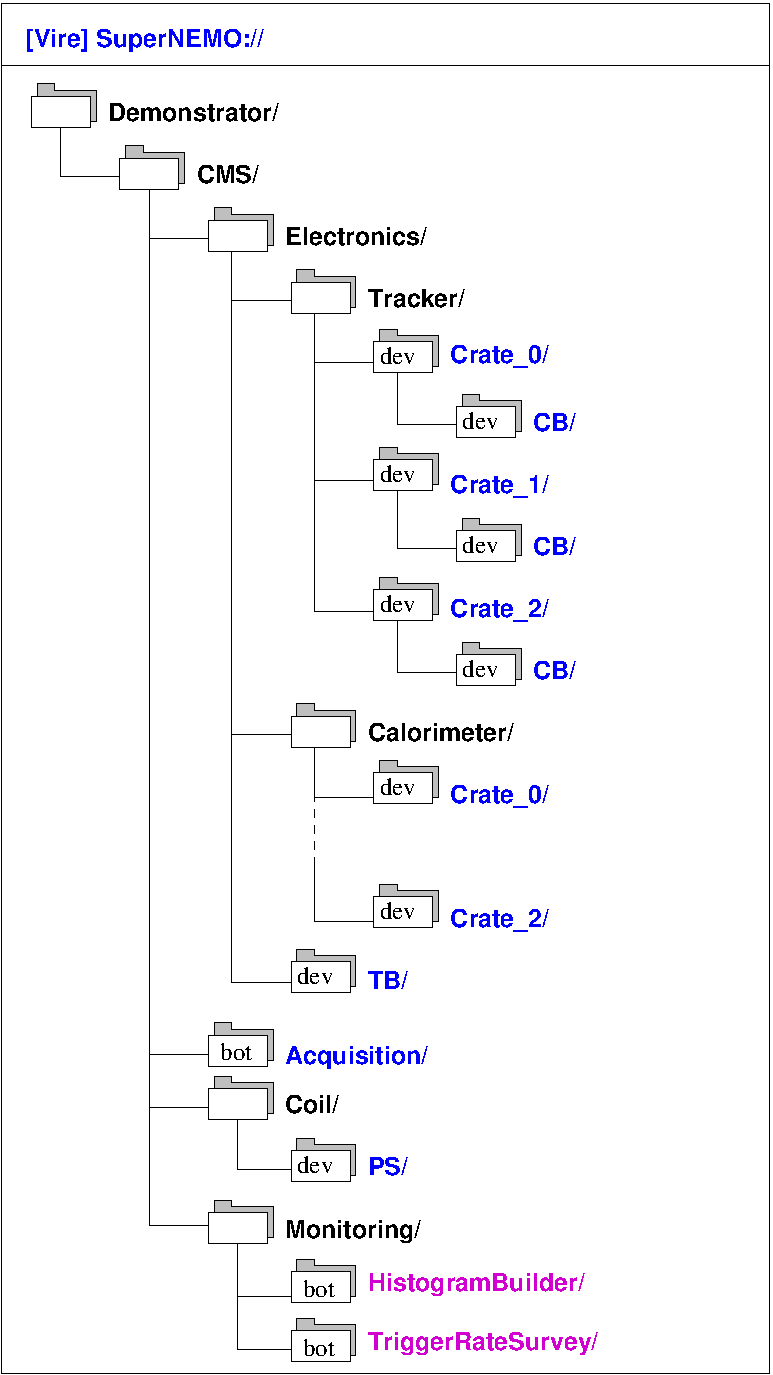
\includegraphics[width=5cm]{appendix/images/MOS_device_example_2.pdf}
\end{center}
\caption{Example of a hierarchy of  devices described by the Vire API.
  The root device is named  \texttt{SuperNEMO:}.  The top level (root)
  device  is  named  \texttt{Demonstrator}.  The  devices  colored  in
  \textcolor{blue}{blue}  are managed  through MOS/OPCUA.  The devices
  colored in \textcolor{magenta}{magenta} are directly embedded in the
  Vire server.  Devices with the \texttt{dev} tag are typical hardware
  device.  Devices  with the  \texttt{bot}  tag  are typical  software
  devices.   The  devices  colored in  \textbf{black}  are  structural
  pseudo-devices used to organize and  present a comprehensive view of
  the hierarchy. }\label{fig:an:mos_dev_2}
\end{figure}

The organisation of this hierarchy of devices is arbitrary and defined
by the designer of the  \emph{Control and Monitoring System}.  What is
important  to  understand  is  that  some  of  these  devices  can  be
associated  to  \emph{hardware  devices}  (a  power  supply  crate,  a
temperature probe\dots) and others  can be \emph{pseudo-devices}, i.e.
pure   software  object   (a   monitoring  robot,   a  file   transfer
daemon\dots).

In the context of the coupling of  the Vire server and the CMS server,
we are  in the event that  some devices are managed  by some MOS/OPCUA
servers and others are managed  in the Vire server itself.  Typically,
\emph{hardware devices}  are systematically managed through  the OPCUA
technology.  Vire has a mechanism to integrate such devices in its own
hierarchy.  This mechanism can  be considered like the \emph{mounting}
of   a   remote   filesystem   from  a   local   filesystem.    Figure
\ref{fig:an:mos_dev_0} illustrates  the case of many  hardware devices
-- managed by MOS -- that are integrated in the Vire system.  From the
Vire point of  view, the user does not see  the implementation details
for such  devices. He  does not  know the identity  of the  MOS server
hosting the device. He does not even know if the device is hosted by a
MOS server.  Devices are simply visible through the standard hierarchy
published by Vire with its  own device naming scheme, regardless their
true location.



\begin{figure}[h]
\begin{center}
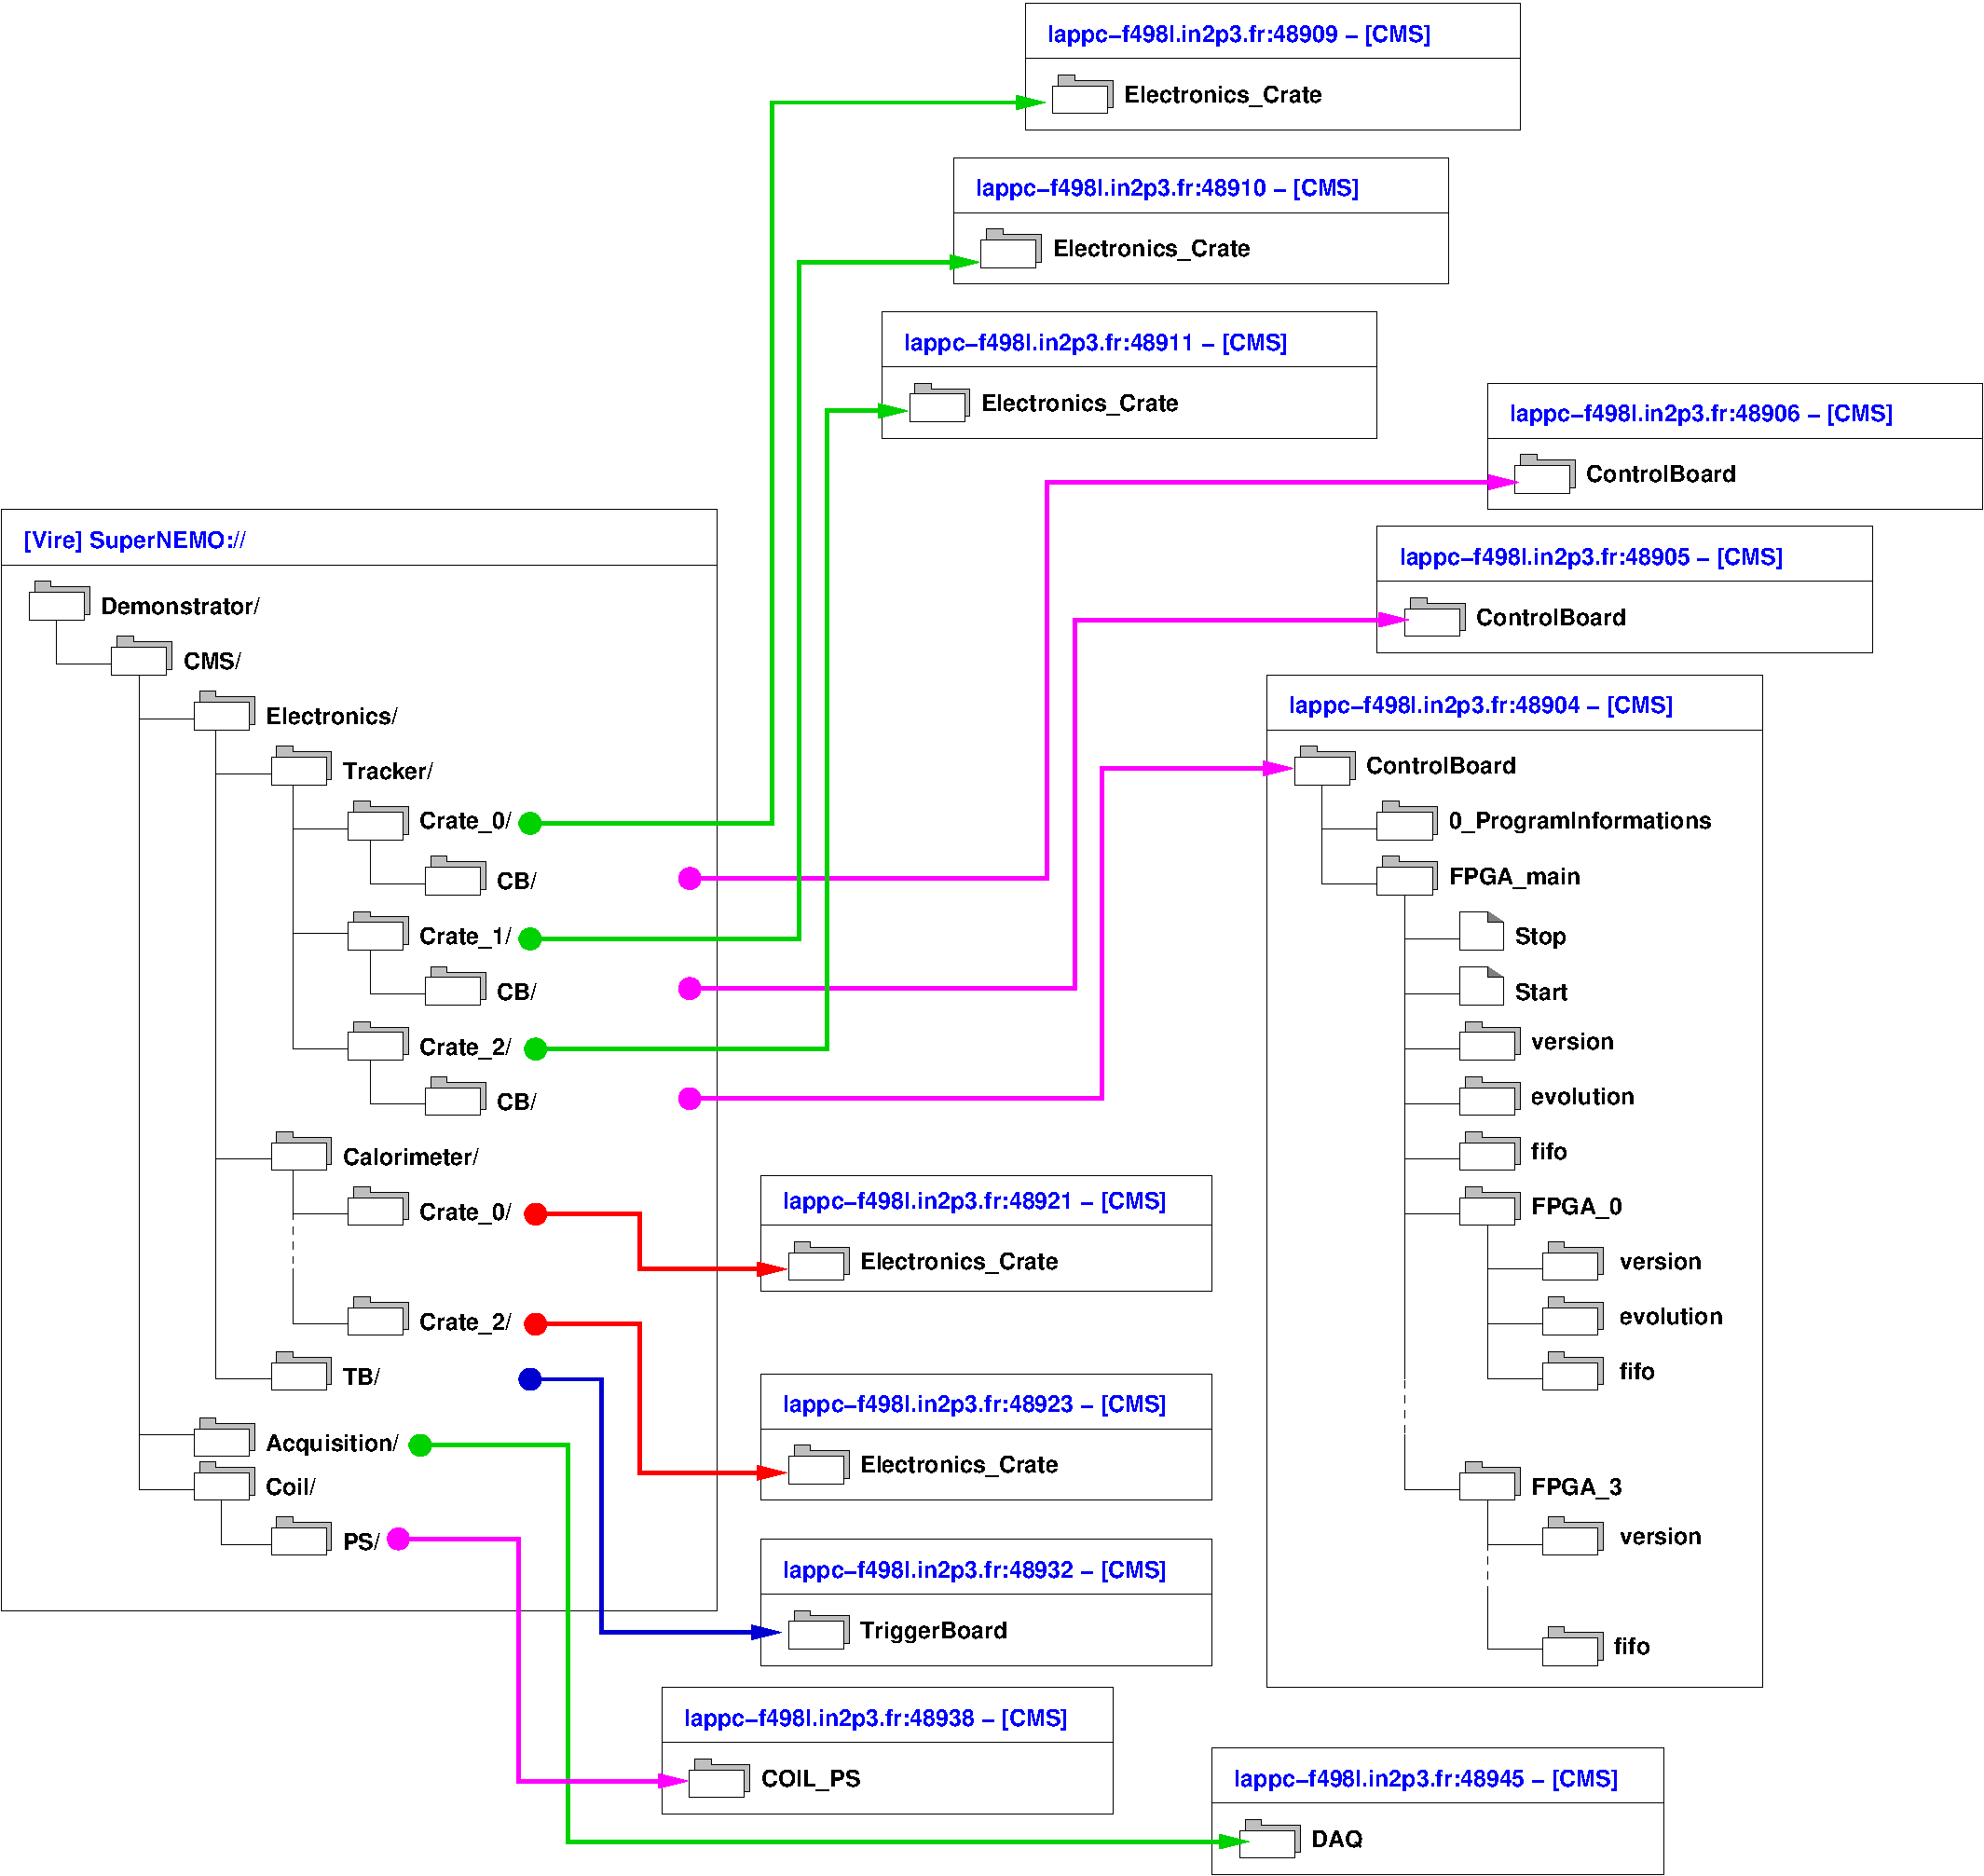
\includegraphics[width=\linewidth]{appendix/images/MOS_device_example_0.pdf}
\end{center}
\caption{The  mounting of  many  MOS device  hierarchies  in the  Vire
  device hierarchy.  Each OPCUA server  runs a simple  hardware device
  that is \emph{mounted} from a specific node with its own path.
%% of  devices described by the Vire API.
%%   The root device is named  \texttt{SuperNEMO:}.  The top level (root)
%%   device is  named \texttt{Demonstrator}. The devices  colored in blue
%%   are managed  through MOS/OPCUA. The  devices colored in  magenta are
%%   directly embedded in the Vire server.  Devices with the \texttt{dev}
%%   tag are typical  hardware device. Devices with  the \texttt{bot} tag
%%   are typical software devices.
}\label{fig:an:mos_dev_0}
\end{figure}




\subsection{Example}

Using  the examples  displayed  in  figure \ref{fig:an:mos_dev_0},  we
consider  in detail  the way  one specific  device managed  by MOS  is
mounted   in  the   Vire   hierarchy.  Figure   \ref{fig:an:mos_dev_3}
illustrates the mounting of a MOS device in Vire.

Here the Vire  server publishes the path of a  device representing the
control board  of the third  electronic crate  for the tracker  of the
SuperNEMO demonstrator module.  The full Vire path of this device is:

\textcolor{blue}{\texttt{SuperNEMO://Demonstrator/CMS/Electronics/Tracker/Crate\_2/CB}}

This is  the only Vire identifier  recognized by user to  address this
device.

On    the   figure,    one    can   see    that    the   MOS    server
\texttt{lappc−f498l.in2p3.fr} (port 48904) hosts a simple device which
is locally named \texttt{ControlBoard}.

When  mounting   this  device  in   the  Vire  hierarchy,   the  local
\texttt{[CMS]}  namespace and  \texttt{ControlBoard} device  names are
hidden and replaced by the Vire device path.  All daughter devices and
datapoints of  the \texttt{CMS/ControlBoard} device are  integrated as
daughters        of        the         Vire        device        named\\
\texttt{SuperNEMO://Demonstrator/CMS/Electronics/Tracker/Crate\_2/CB}.


For example, the \texttt{FPGA\_main} daughter device is now associated
to the following Vire path:

\textcolor{blue}{\texttt{SuperNEMO://Demonstrator/CMS/Electronics/Tracker/Crate\_2/CB/FPGA\_main/}}

and  its  \texttt{Stop} method  is  automatically  addressed with  the
following \emph{leaf} path:

\textcolor{blue}{\texttt{SuperNEMO://Demonstrator/CMS/Electronics/Tracker/Crate\_2/CB/FPGA\_main/Stop}}


\begin{figure}[h]
\begin{center}
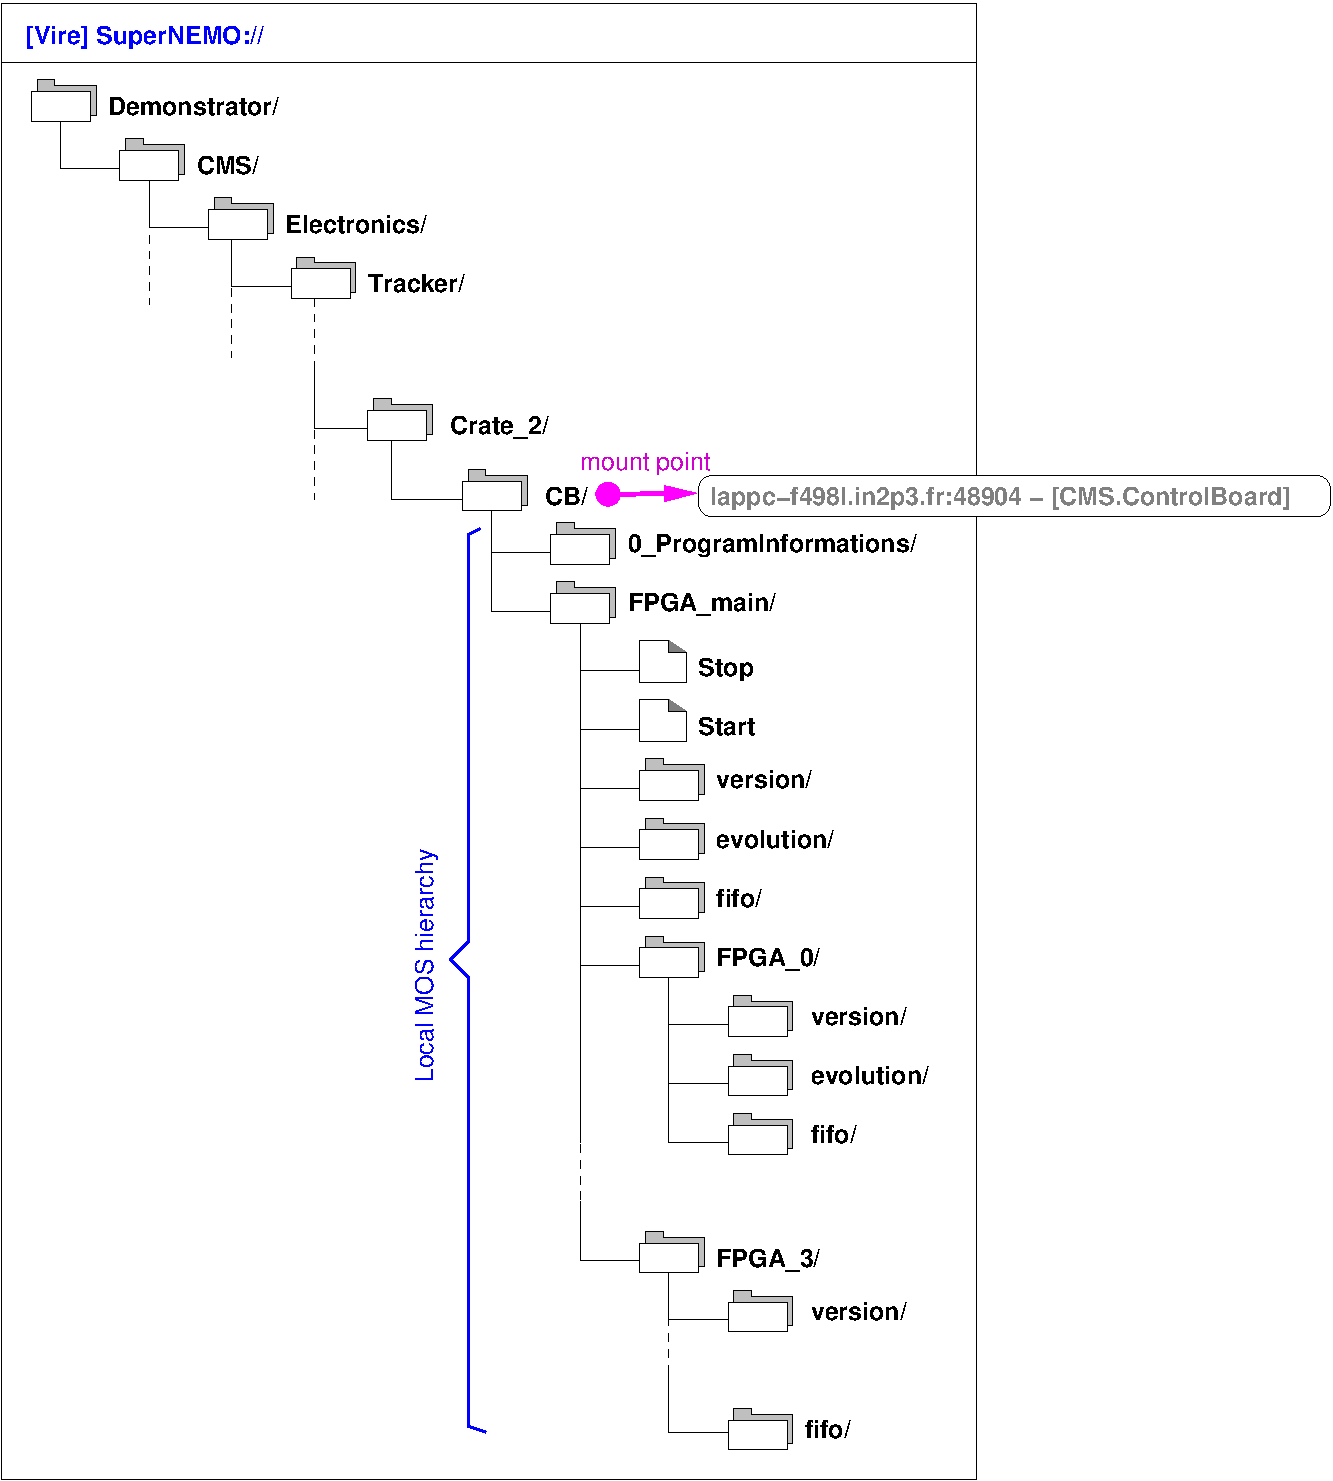
\includegraphics[width=0.8\linewidth]{appendix/images/MOS_device_example_3.pdf}
\end{center}
\caption{The  mounting of  one  MOS device and its local hierarchy  in the  Vire
  device hierarchy.}\label{fig:an:mos_dev_3}
\end{figure}



\subsection{Vire/MOS mapping}

As it can be  seen in the above example, the integration  of a new MOS
device in the Vire system is  achieved through soem kind of filesystem
mounting operation.   Particularly, it is  shown that the MOS  name of
the   mounted  root   device  is   replaced  by   an  arbitrary   Vire
path. However, all daughter  nodes (devices, datapoints) attached from
this root  node have their  relative MOS  names preserved in  the Vire
naming scheme.

Any  resource  (method)  associated  to any  of  such  daughter  nodes
inherits this relative naming scheme.

As Vire applications  describe resources through their  Vire paths, it
is thus needed to build an explicit map that associates resource paths
to MOS address  and name. The CMS  server will be able  to resolve the
MOS server/port and  embedded device associated to  the resource path.

The goal of the \texttt{devices\_launch.conf} file is not only to tell
the CMS server what MOS server should  be loaded and ran at start, but
also  to describe  the  \emph{mounting point/names}  used  by Vire  to
access the resources associated to MOS devices.  From the informations
stored in the  file, an explicit associative array must  be built when
the Vire server connect to the CMS server.  It will play the role of a
resource path resolver  when requests about resources will  be sent by
Vire applications.  This associative array  must be locked  during the
Vire/CMS connection.



%\subsubsection{Preparation of XML device models}

%% \noindent\underline{Pre-condition:}
%% The device is working and validated through the MOS/OPCUA server

%% \begin{enumerate}

%% \item Produce XML décrivant le modèle du device enrichi
%%   des metadata
%% Rédaction du fichier XML décrivant le modèle du device

%% \item Génération des fichiers model du type de device pour Vire

%% \item Génération des fichiers instances resolv.conf

%% \end{enumerate}


\vfill
\pagebreak
\clearpage

% end


\section{Vire messages}\label{app:vire_messages}

Within Vire  and between Vire  components and external  components, we
use  a communication  system  based on  Vire  messages.  This  section
describes the structure of such messages.

\subsection{General structure of a message}

Each message consists in two parts (figure \ref{fig-vire-message-message-cpp}):
\begin{itemize}

\item  the  \emph{header}  is   dedicated  to  generic  and  typicalle
  mandatory  informations  which  document   the  message  itself  and
  arbitrary high-level metadata.

\item  the \emph{body}  of the  message  contains the  real data: the payload.
  The structure of the message body depends on some convention. Vire uses
  its own convention to embed the payload data.

\end{itemize}

\begin{figure}[h]
\vskip 10pt
\small
\begin{Verbatim}[frame=single,xleftmargin=0.cm,label=\fbox{C++}]
struct vire::message::message {
  message_header header; // Header of the message
  message_body   body;   // Body of the message
};
\end{Verbatim}
\normalsize
\caption{The structure of a Vire message object (C++  class:
  \texttt{"vire::message::message"})}\label{fig-vire-message-message-cpp}
\end{figure}

\subsection{The message header}

The header contains (figure \ref{fig-vire-message-message_header-cpp}):
\begin{itemize}

  \item The mandatory \texttt{message\_id}  attribute is an identifier
    of the  message which  document the emitter  and a  unique message
    number.   Each emitter  is  responsible of  the  numbering of  the
    messages it  emits, typically using an  incremental technique. The
    message  number is  a positive  integer, starting  from 0  (figure
    \ref{fig-vire-message-message_identifier-cpp}).

  \item  The \texttt{timestamp}  attribute  encodes the  approximative
    time point when the message was  created. It contains the date and
    the time, using at least microsecond resolution.

    Typically,  with  JSON  encoding  system, it  is  expected  to  be
    formatted as a character string, using the following ISO format:

    \begin{center}
      \texttt{yyyymmddThhmmss.uuuuuu}
    \end{center}

    \noindent where:

    \vskip -10pt
    \begin{itemize}
    \item[\texttt{yyyymmdd} :] encodes year/month/day,
    \item[\texttt{hhmmssd} :] encodes hour/minute/second,
    \item[\texttt{uuuuuu} :] encodes microseconds.
    \end{itemize}

  \item   In   the   case    of   a   \emph{response}   message,   the
    \texttt{in\_reply\_to} attribute is set to identify the associated
    request message.

  \item  The \texttt{asynchronous}  boolean  attribute is  set if  the
    message processing  is explicitely requested  by the source  to be
    asynchronous (non-blocking).  In  RPC transactions, where requests
    are transmitted from one point to  the other, its default value is
    \emph{false}.   It  is possible  to  force  a RPC  transaction  in
    asynchronous mode.   This use  case is documented  elsewhere.  For
    event messaging, this flag is conventionally set to \emph{true}.

  \item  The  \texttt{body\_layout\_id}  attribute  is  the  mandatory
    identifier   of   the   layout   of  the   message   body   (class
    \texttt{"vire::utility::model\_identifier"}).  The  default layout
    for     message     body     inside    the     Vire     API     is
    \texttt{"vire::message::body\_format::typed\_payload"}, with version
    \texttt{"1.0"}                                             (figure
    \ref{fig-vire-utility-model_identifier-cpp}).

\end{itemize}


\begin{figure}[h]
\vskip 10pt
\small
\begin{Verbatim}[frame=single,xleftmargin=0.cm,label=\fbox{C++}]
struct vire::message::message_header {
  message_identifier message_id;     // Message identifier from the emitter.
  std::string        timestamp;      // Timestamp.
  message_identifier in_reply_to;    // Message identifier of the associated
                                     // request message (optional).
  bool               asynchronous,   // Asynchronous flag.
  vire::utility::model_identifier     body_layout_id; // Body layout identifier.
  std::map<std::string, std::string>  metadata;       // Key/value metadata dictionary.
};
\end{Verbatim}
\normalsize
\caption{The  structure  of  a   message  header  object  (C++  class:
  \texttt{"vire::message::message\_header"}).}\label{fig-vire-message-message_header-cpp}
\end{figure}

\begin{figure}[h]
\vskip 10pt
\small
\begin{Verbatim}[frame=single,xleftmargin=0.cm,label=\fbox{C++}]
struct vire::message::message_identifier {
  std::string emitter; // Name identifying the emitter of the message.
  int32_t     number;  // Number identifying the message in the emitter's
                       // message numbering scheme.
};
\end{Verbatim}
\normalsize
\caption{The      structure      of     a      message      identifier
  (C++  class:  \texttt{"vire::message::message\_identifier"}).}
\label{fig-vire-message-message_identifier-cpp}
\end{figure}

\begin{figure}[h]
\vskip 10pt
\small
\begin{Verbatim}[frame=single,xleftmargin=0.cm,label=\fbox{C++}]
struct vire::utility::model_identifier {
  std::string name;    // Name identifying the format of the message.
  std::string version; // String identifying the version of the format.
};
\end{Verbatim}
\normalsize
\caption{The structure of a model identifier (C++  class:  \texttt{"vire::utility::model\_identifier"}.}\label{fig-vire-utility-model_identifier-cpp}
\end{figure}




\begin{figure}[h]
\vskip 10pt
\small
\begin{Verbatim}[frame=single,xleftmargin=0.cm,label=\fbox{JSON}]
{
   "header" : {
      "message_id" : {
         "emitter" : "vire.server",
         "number" : 42
      },
      "timestamp" : "20160930T141408.413443",
      "in_reply_to" : {
         "initialized" : true,
         "value" : {
            "emitter" : "vire.client.0",
            "number" : 23
         }
      },
      "asynchronous" : false,
      "body_layout_id" : {
         "name" : "vire::message::body_format::typed_payload",
         "version" : {
            "initialized" : true,
            "value" : "1.0"
         }
      },
      "metadata" : [
         {
            "key" : "key1",
            "value" : "foo"
         },
         {
            "key" : "key2",
            "value" : "42"
         },
         {
            "key" : "key3",
            "value" : "3.1415899999999999"
         },
         {
            "key" : "key4",
            "value" : "true"
         }
      ]
   }
  "body" : {
      ...
   }
}
\end{Verbatim}
\normalsize
\caption{Example of  a   message  header  object in JSON format.}
\label{fig-vire-message-message_header-json}
\end{figure}

\vfill
\clearpage
\pagebreak

\subsection{The message body}

The    default    message   body    layout    in    Vire   is    named
\texttt{"vire::message::body\_format::typed\_payload"}        (version
\texttt{"1.0"}).   Each  message used  within  the  Vire framework  is
supposed to use this layout.  The general idea is that the body of the
message embeded the  \emph{payload object} that has  to be transmitted
between  two components  of  the system.   \emph{Payload objects}  are
classified in one of the three following categories:

\begin{enumerate}

\item \emph{Request}:  describes a request submitted  by one component
  to another component (generally during a synchronous RPC transaction).

\item  \emph{Response}: describes  the  response to  a former  request
  (generally during a synchronous RPC transaction).

\item \emph{Event}: describes an  arbitrary information record (alarm,
  exception, signal\dots) which is transmitted asynchronously.

\end{enumerate}

Vire implements the following class hierarchy:

\begin{center}
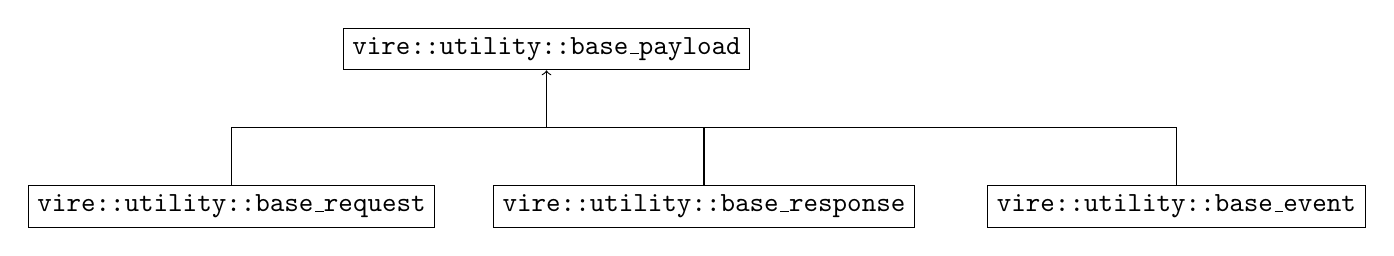
\begin{tikzpicture}
  \node (payload)  at (0,2)  [draw] {\texttt{vire::utility::base\_payload}};
  \node (request)  at (-4,0) [draw] {\texttt{vire::utility::base\_request}};
  \node (response) at (2,0)  [draw] {\texttt{vire::utility::base\_response}};
  \node (event)    at (8,0)  [draw] {\texttt{vire::utility::base\_event}};

  %\draw[style=help lines] (-3,-1) grid (10,4);
  \draw (node cs:name=response,anchor=north) |- (0,1);
  \draw (node cs:name=event,anchor=north)    |- (0,1);
  \draw[->] (node cs:name=request,anchor=north)
  |- (0,1) -| (node cs:name=payload,anchor=south);
\end{tikzpicture}
\end{center}

The requirements for the transmitted object are the following:

\begin{itemize}

\item The  type of the object  must be conventionally associated  to a
  unique     \emph{model      identifier}     object      (see     the
  \texttt{"vire::utility::model\_identifier"} class)  which contains a
  unique   name   (\textit{string    identifier})   and   possibly   a
  \textit{version identifier}.  Each software  component that may send
  or  receive the  object  should agree  on  this type  identification
  scheme.   This   enable  the  use  of   object  factories,  whatever
  programming  langage  is used  on  both  side of  the  communication
  system.

\item  For each  software component,  the object  type must  have some
  dedicated  encoding/decoding  functions  available  (again  whatever
  programming language is used). For example the Vire API supports the
  following encoding formats:

  \begin{itemize}

  \item JSON (MIME  encoding type: \texttt{"application/x-json"}), which
    is supportable by many languages,

  \item  Protobuf  (Google  Protocol   Buffers,  MIME  encoding  type:
    \texttt{"application/x-protobuf"}), which is also widely supported,

  \item   Boost/serialisation   (XML,    text   or   binary   archives
    \texttt{"application/x-boost-serialization-xml"},
    \texttt{"application/x-boost-serialization-text"},
    \texttt{"application/x-boost-serialization-binary"}),    which    in
    principle is supported by C++ only.

  \end{itemize}

  The Protobuf  encoding format will be  used to serialize/deserialize
  the  Vire  messages transported  between  the  Vire server  and  the
  CMS/LAPP server.

\end{itemize}

Vire uses a dedicated layout to represent the body of any message with
its embedded payload object. With this technique, the structure of the
body          contains         two          attributes         (figure
\ref{fig-app-vire-message-message_body-cpp}):

\begin{enumerate}

\item The \texttt{payload\_type\_id} specifies the type of the payload
  object   (figure   \ref{fig-app-vire-utility-model_identifier-cpp}).
  This unique name  is conventionaly fixed for a  given application. A
  version tag allows to support possible evolution of the object type.

\item The  \texttt{payload} is a  handle to  a payload object  of type
  request, response or event.

  %% \begin{itemize}
  %% \item Within  the producer  component of  the message,  the encoding
  %%   function associated to the object  type is responsible to generate
  %%   the JSON stream for the object and store it in the buffer.

  %% \item Within  the consumer  component of  the message,  the decoding
  %%   function associated to the object type is responsible to parse the
  %%   JSON stream stored in the buffer and restore the object in memory.

  %% \end{itemize}

  It is expected  that, on both sides of the  connection, the software
  components can  access dedicated  software plugins which  ensure the
  support  of  various   \emph{payload  object  types}  conventionnaly
  associated  with  their  \emph{payload type  identifiers}  and  also
  providing JSON and/or Protobuf encoding/decoding functionalities.

  %% The   system  allows  to  support
  %% modification  in the  structure of  the objects  thanks to  version
  %% tagging.

\end{enumerate}

\begin{figure}[h]
\vskip 10pt
\small
\begin{Verbatim}[frame=single,xleftmargin=0.cm,label=\fbox{C++}]
struct message_body {
  vire::utility::model_identifier     payload_type_id; // Object type identifier.
  const vire::utility::base_payload * payload;         // Handle to a payload object.
};
\end{Verbatim}
\normalsize
\caption{The structure of a message body object (C++).}
\label{fig-app-vire-message-message_body-cpp}
\end{figure}

\begin{figure}[h]
\vskip 10pt
\small
\begin{Verbatim}[frame=single,xleftmargin=0.cm,label=\fbox{JSON}]
{
  "header" : {
    ...
  },
  "body" : {
    "payload_type_id" : {
      "name" : "vire::message::testing::error_event",
      "version" : {
        "initialized" : false
      }
    },
    "payload" : {
      "timestamp" : "20160930T141743.759085"
      "err" : {
        "code" : 3,
        "message" : "A basic error"
      },
    }
  }
}
\end{Verbatim}
\normalsize
\caption{Example of  a   message  body  object in JSON format.}
\label{fig-vire-message-message_body-json}
\end{figure}

\vfill
\clearpage
\pagebreak

% end

%\input{appendix/app_json_fmt.tex}

\section{The \emph{Protocol Buffers} format}\label{app:protobuf_fmt}

\subsection{Introduction}

The  Google  Protocol Buffers  (\emph{protobuf})  library  is used  to
represent the objects that are exchanged between the Vire clients, the
Vire server and the CMS server.  The  version 3 of the format is used,
implying   at   least   version   3.0.0  (September   2016)   of   the
\emph{protobuf} library.

Each  data   structure  of  interest   can  be  described   through  a
\texttt{.proto}  file  from  which  stub files  can  be  automatically
generated  with the  \texttt{protoc} compiler.  For Vire  and its  CMS
interface, the C++ and Java programming languages will be used.


A  collection of  \texttt{.proto}  files are  provided  with the  Vire
library to represent all kind  of data structures transferable between
networked agents  (Vire server,  Vire clients, CMS/LAPP  server).  The
objects of  the highest level  are named \emph{payload  objects} (like
\emph{request},  \emph{response} and  \emph{event} objects).   They
are composed of attributes of more basic data structures.

\subsection{Example}

The following  class diagram  illustrates two data  structures defined
within the Vire library with an inheritance relationship between them.

\begin{center}
  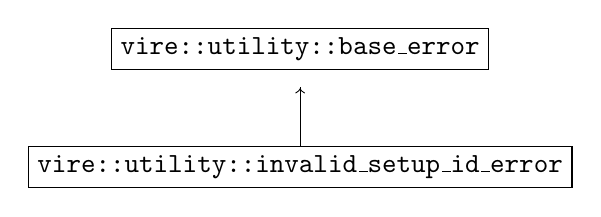
\begin{tikzpicture}
    \node (base)     at (0,1.5)  [draw] {\texttt{vire::utility::base\_error}};
    \node (setup)    at (0,0)  [draw] {\texttt{vire::utility::invalid\_setup\_id\_error}};

    \draw[->]   (node cs:name=setup,anchor=north) |- (0,1);
    |- (0,1) -| (node cs:name=base,anchor=south);
  \end{tikzpicture}
\end{center}

The \texttt{vire::utility::base\_error}  is the  parent class  for all
\emph{error}  objects.   It  contains   two  attributes:   an  integer
\emph{error code}  and a  character string describing  the \emph{error
  message}.

The   \texttt{vire::utility::invalid\_setup\_id\_error}  class   is  a
specialized error class  which represents explicitely an  error due to
an identification  failure of  the experimental setup.   It implements
additional mutually exclusive attributes: the \emph{unrecognized name}
of the setup or the \emph{unrecognized version} of the setup.

This   example  illustrates   the  protobuf   representation  of   the
\texttt{vire::utility::base\_error}  in the  Vire  library, using  the
\texttt{"vire/utility/BaseError.proto"} file:

\small
\begin{Verbatim}[frame=single,xleftmargin=0.cm,label=\fbox{protobuf}]
  syntax = "proto3";
  package vire.utility; // Namespace

  message BaseError {

    // reserved 1; // Reserved for _base message

    // Attributes:
    int32  code           = 100; // The error code
    string message_format = 101; // The error description message

  }
\end{Verbatim}
\normalsize

\vfill
\clearpage
\pagebreak

\subsection{Vire protobuf conventions}

Vire uses the following conventions:

\begin{enumerate}

\item
  The member index  \texttt{1} is reserved to represent the  link of a
  class to its main base/parent class (if any).  It is not used if the
  data structure does not inherit any data structure.
  If a data structure naturally inherits another one, it is thus possible
  to  represent the  inheritance  relationship as  illustrated with  the
  \texttt{"vire/utility/InvalidSetupIdError.proto"}      file      which
  represents the \texttt{vire::utility::invalid\_setup\_id\_error} class
  in the Vire library:

  \small
  \begin{Verbatim}[frame=single,xleftmargin=0.cm,label=\fbox{protobuf}]
    syntax = "proto3";
    package vire.utility; // Namespace

    import "vire/utility/BaseError.proto"; // Dependency

    message InvalidSetupIdError {

      BaseError _base = 1; // The base class

      // Additional attributes:
      oneof detail { // Mutual exclusion
        string invalid_setup_name    = 100; // The failed setup name
        string invalid_setup_version = 101; // The failed setup version
      }

    }
  \end{Verbatim}
  \normalsize

\item The  \texttt{\_base} member  is conventionally  used to  represent the
  inheritance   relationship    from   a   data   structure    of   type
  \texttt{"vire.utility.BaseError"}.

\item Member indexes from \texttt{2}  to \texttt{99} are also reserved
  for possible future usage (multiple inheritance, metadata\dots).

\item
  The first member of the data structure must start at index \texttt{100}.

\end{enumerate}

\vfill
\clearpage
\pagebreak

% end


\section{Vire payload objects}\label{app:payload}

\subsection{Introduction}

As  mentioned in  appendix \ref{app:protobuf_fmt},  Vire messages  are
wrappers for \emph{payload objects}.  Each  type of payload object can
be represented  through the \emph{protobuf} mechanism.   The following
class hierarchy shows the base architecture used to define new payload
objects.

\begin{center}
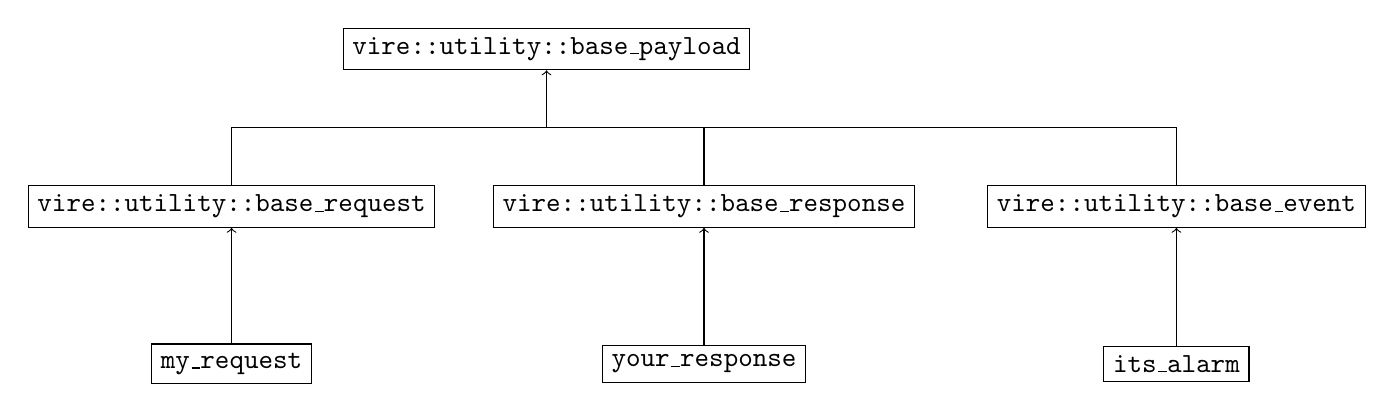
\begin{tikzpicture}
  \node (payload)  at (0,2)   [draw] {\texttt{vire::utility::base\_payload}};
  \node (request)  at (-4,0)  [draw] {\texttt{vire::utility::base\_request}};
  \node (response) at (2,0)   [draw] {\texttt{vire::utility::base\_response}};
  \node (event)    at (8,0)   [draw] {\texttt{vire::utility::base\_event}};
  \node (my)       at (-4,-2) [draw] {\texttt{my\_request}};
  \node (your)     at (2,-2)  [draw] {\texttt{your\_response}};
  \node (its)    at (8,-2)    [draw] {\texttt{its\_alarm}};

  %\draw[style=help lines] (-6,-2) grid (10,2);
  \draw (node cs:name=response,anchor=north) |- (0,1);
  \draw (node cs:name=event,anchor=north)    |- (0,1);
  \draw[->] (node cs:name=request,anchor=north)
  |- (0,1) -| (node cs:name=payload,anchor=south);
  \draw[->] (node cs:name=my,anchor=north)
  |- (-4,-1) -| (node cs:name=request,anchor=south);
  \draw[->] (node cs:name=your,anchor=north)
  |- (2,-1) -| (node cs:name=response,anchor=south);
  \draw[->] (node cs:name=its,anchor=north)
  |- (8,-1) -| (node cs:name=event,anchor=south);
\end{tikzpicture}
\end{center}


\begin{center}
\vskip 10pt
\small
\begin{tabular}{|l|l|l|}
  \hline
  \textbf{Vire C++ class} & \textbf{protobuf message type} & \textbf{protobuf definition file} \\
  \hline
  \hline
  \multicolumn{3}{|c|}{\emph{general types}} \\
  \hline
  boost::posix\_time::ptime & google.protobuf.Timestamp & google/protobuf/timestamp.proto \\
  \hline
  \hline
  \multicolumn{3}{|c|}{\emph{identifier types}} \\
  \hline
  vire::utility::base\_identifier & vire.utility.Baseidentifier & vire/utility/Baseidentifier.proto \\
  \hline
  vire::utility::instance\_identifier & vire.utility.InstanceIdentifier & vire/utility/InstanceIdentifier.proto \\
  \hline
  vire::utility::model\_identifier & vire.utility.ModelIdentifier & vire/utility/ModelIdentifier.proto \\
  \hline
  \hline
  \multicolumn{3}{|c|}{\emph{error types}} \\
  \hline
  vire::utility::base\_error & vire.utility.BaseError & vire/utility/BaseError.proto \\
  \hline
  vire::utility::invalid\_context\_error & vire.utility.InvalidContextError & vire/utility/InvalidContextError.proto \\
  \hline
  vire::utility::invalid\_setup\_id\_error & vire.utility.InvalidSetupIdError & vire/utility/InvalidSetupIdError.proto \\
  \hline
  \hline
  \multicolumn{3}{|c|}{\emph{payload types}} \\
  \hline
  vire::utility::base\_payload & vire.utility.BasePayload & vire/utility/BasePayload.proto \\
  \hline
  vire::utility::base\_request & vire.utility.BaseRequest & vire/utility/BaseRequest.proto \\
  \hline
  vire::utility::base\_response & vire.utility.BaseResponse & vire/utility/BaseResponse.proto \\
  \hline
  vire::utility::base\_event & vire.utility.BaseEvent & vire/utility/BaseEvent.proto \\
  \hline
  vire::utility::base\_alarm & vire.utility.BaseAlarm & vire/utility/BaseAlarm.proto \\
  \hline
  \hline
  \multicolumn{3}{|c|}{\emph{messenging types}} \\
  \hline
  vire::message::message\_identifier & vire.message.MessageIdentifier & vire/message/MessageIdentifier.proto \\
  \hline
  vire::message::msg\_header & vire.message.MsgHeader & vire/message/MsgHeader.proto \\
  \hline
  vire::message::msg\_body & vire.message.MsgBody & vire/message/MsgBody.proto \\
  \hline
  vire::message::message & vire.message.Message & vire/message/Message.proto \\
  \hline
\end{tabular}
\normalsize
\end{center}


\begin{center}
\vskip 10pt
\small
\begin{tabular}{|l|l|l|}
  \hline
  \multicolumn{3}{|c|}{\emph{Resource management related types}} \\
  \hline
  vire::cms::resource\_status\_record & vire.cms.ResourceStatusRecord & vire/cms/ResourceStatusRecord.proto \\
  \hline
  vire::cms::resource\_fetch\_status\_request & vire.cms.ResourceFetchStatusRequest & vire/cms/ResourceFetchStatusRequest.proto \\
  \hline
  vire::cms::resource\_fetch\_status\_success\_response & vire.cms.ResourceFetchStatusSuccessResponse & vire/cms/ResourceFetchStatusSuccessResponse.proto \\
  \hline
  vire::cms::resource\_fetch\_status\_failure\_response & vire.cms.ResourceFetchStatusFailureResponse & vire/cms/ResourceFetchStatusFailureResponse.proto \\
  \hline
  vire::cms::resource\_exec\_request & vire.cms.ResourceExecRequest & vire/cms/ResourceExecRequest.proto \\
  \hline
  vire::cms::resource\_exec\_success\_response & vire.cms.ResourceExecSuccessResponse & vire/cms/ResourceExecSuccessResponse.proto \\
  \hline
  vire::cms::resource\_exec\_failure\_response & vire.cms.ResourceExecFailureResponse & vire/cms/ResourceExecFailureResponse.proto \\
  \hline
  vire::cms::resource\_exec\_non\_blocking\_request & vire.cms.ResourceExecNonBlockingRequest & vire/cms/ResourceExecNonBlockingRequest.proto \\
  \hline
  vire::cms::resource\_exec\_non\_blocking\_ack\_response & vire.cms.ResourceExecNonBlockingAckResponse & vire/cms/ResourceExecNonBlockingAckResponse.proto \\
  \hline
  vire::cms::resource\_exec\_non\_blocking\_noack\_response & vire.cms.ResourceExecNonBlockingNoackResponse & vire/cms/ResourceExecNonBlockingNoackResponse.proto \\
  \hline
  vire::cms::resource\_exec\_non\_blocking\_success\_event & vire.cms.ResourceExecNonBlockingSuccessEvent & vire/cms/ResourceExecNonBlockingSuccessEvent.proto \\
  \hline
  vire::cms::resource\_exec\_non\_blocking\_failure\_event & vire.cms.ResourceExecNonBlockingFailureEvent & vire/cms/ResourceExecNonBlockingFailureEvent.proto \\
  \hline
  vire::cms::resource\_exec\_error & vire.cms.ResourceExecError & vire/cms/ResourceExecError.proto \\
  \hline
  vire::cms::invalid\_status\_error & vire.cms.ResourceExecError & vire/cms/ResourceExecError.proto \\
  \hline
  %% vire::cms::invalid\_credentials\_error & vire.cms.InvalidCredentialsError & vire/cms/InvalidCredentialsError.proto \\
  %% \hline
  %% vire::cms::invalid\_user\_error & vire.cms.InvalidUserError & vire/cms/InvalidUserError.proto \\
  %% \hline
  vire::cms::invalid\_resource\_error & vire.cms.InvalidUserError & vire/cms/InvalidUserError.proto \\
  \hline
  vire::cms::no\_pubsub\_resource\_error & vire.cms.NoPubsubResourceError & vire/cms/NoPubsubResourceError.proto \\
  \hline
  \hline
  \multicolumn{3}{|c|}{\emph{Resource pub/sub management types}} \\
  \hline
  vire::cms::resource\_pubsub\_subscribe\_request & vire.cms.ResourcePubsubSubscribeRequest & vire/cms/ResourcePubsubSubscribeRequest.proto \\
  \hline
  vire::cms::resource\_pubsub\_subscribe\_success\_response & vire.cms.ResourcePubsubSubscribeRSuccessResponse & vire/cms/ResourcePubsubSubscribeRSuccessResponse.proto \\
  \hline
  vire::cms::resource\_pubsub\_subscribe\_failure\_response & vire.cms.ResourcePubsubSubscribeRFailureResponse & vire/cms/ResourcePubsubSubscribeRSuccessResponse.proto \\
  \hline
  \hline
  \multicolumn{3}{|c|}{\emph{Vire/CMS server interface types}} \\
  \hline
  vire::cmsinterface::connection\_request & vire.cmsinterface.ConnectionRequest & vire/cmsinterface/ConnectionRequest.proto \\
  \hline
  vire::cmsinterface::connection\_success\_response & vire.cmsinterface.ConnectionSuccessResponse & vire/cmsinterface/ConnectionSuccessResponse.proto \\
  \hline
  vire::cmsinterface::connection\_failure\_response & vire.cmsinterface.ConnectionFailureResponse & vire/cmsinterface/ConnectionFailureResponse.proto \\
  \emph{embedded:} unknown\_resources\_error & .UnknownResourcesError &  \\
  \hline
  vire::cmsinterface::disconnection\_request & vire.cmsinterface.DisconnectionRequest & vire/cmsinterface/DisconnectionRequest.proto \\
  \hline
  vire::cmsinterface::disconnection\_success\_response & vire.cmsinterface.DisconnectionSuccessResponse & vire/cmsinterface/DisconnectionSuccessResponse.proto \\
  \hline
  %% \hline
  %% vire::cmsinterface::disconnection\_failure\_response & vire.cmsinterface.DisconnectionFailureResponse & vire/cmsinterface/DisconnectionFailureResponse.proto \\
\end{tabular}
\normalsize
\end{center}

\subsection{Basic data structures}

Any  payload object  (request, response  or event)  generally contains
some information records which are  specific to the functionalities of
the  payload  object they  belong.   These  records are  of  arbitrary
types. Of course they should be  translatable in terms of the protobuf
library.
%Of course they can be (de)serialized using JSON.
Some of these types are very  general and defined within the Vire core
API itself because they are reused by various payload objects not only
through  the Vire-CMS/LAPP  interface  but also  between  Vire clients  and
servers, independently  of the  CMS/LAPP server.  However,  the use  of the
Protocol Buffers interface makes possible  to publish the interface of
such data to the outside world, including the CMS/LAPP server in priority.

%% Other one are specific to the Vire/CMS interface and thus managed only
%% in the \texttt{Vire\_CMSInterface} API.
These  types  are considered  as  \emph{basic}.  Among them  we  find:
generic error  types, generic  identifier types,  timestamps, resource
status records\dots We propose to describe them in this section.

Once a sufficient collection of  basic data record types is available,
it  is possible  to describe  high  level payload  object types  which
aggregate attributes of such types.

Other record  types are specific to  some payload objects and  will be
never  used outside  the scope  of these  payload objects.   Such data
structures will be  explicitely declared with the  payload object they
belong to, likely as embedded types/classes.


\subsubsection{Errors}

Some  \emph{response} or  \emph{event} payload  objects may  contain a
specific  error  record  object.   A  \emph{failure  response}  or  an
\emph{exception  event}  object will  generally  embed  such an  error
record object.

Each  \emph{error record}  is represented  by an  instance of  a given
error type.   Each of  the error  types defined  in Vire  inherits the
\texttt{vire::utility::base\_error}      base       class      (figure
\ref{fig-app-payload-base_error})   which   contains   the   following
attributes:

\begin{itemize}

\item the error code: A non zero  integer which is set to 1 by default
  (indicating  a  generic  failure  case).   The  error  code  can  be
  conventionally  set to  any positive  integer value  to represent  a
  specific error case, depending on the context.

\item the error  message: an optional human  readable character string
  which documents the error as usefully as possible.

\end{itemize}

\begin{figure}[h]
\vskip 10pt
\small
\begin{Verbatim}[frame=single,xleftmargin=0.cm,label=\fbox{C++}]
struct vire::utility::base_error
{
  // Attributes:
  int         code;           // Error code (>0).
  std::string message_format; // Error message (optional).
};
\end{Verbatim}
\normalsize
\caption{The structure of a \texttt{"vire::utility::base\_error"} object
  (C++).}
\label{fig-app-payload-base_error}
\end{figure}


%% An example of JSON formatted basic error object is given in figure
%% \ref{fig-app-payload-base_error-1}.
%%
%% \begin{figure}[h]
%% \vskip 10pt
%% \small
%% \begin{Verbatim}[frame=single,xleftmargin=0.cm,label=\fbox{\texttt{JSON}}]
%% {
%%   "code" : "42",
%%   "message_format" : "Invalid AMQP server port=[2341]"
%% }
%% \end{Verbatim}
%% \normalsize
%% \caption{JSON  formatted  basic  error  object  (class
%%   \texttt{vire::utility::base\_error}.}
%% \label{fig-app-payload-base_error-1}
%% \end{figure}

Several type of generic errors are defined in Vire:


\begin{center}
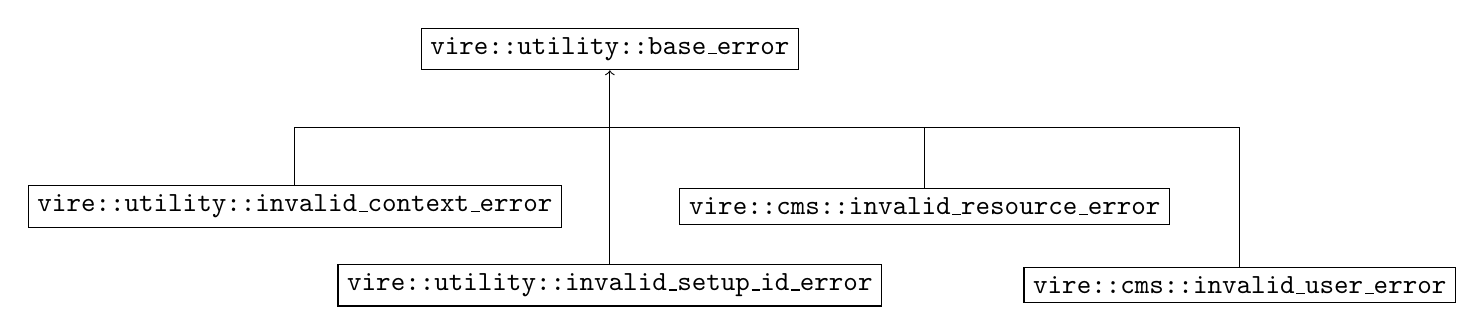
\begin{tikzpicture}
  \node (base)     at (0,2)  [draw] {\texttt{vire::utility::base\_error}};
  \node (context)  at (-4,0) [draw] {\texttt{vire::utility::invalid\_context\_error}};
  \node (setup)    at (0,-1)  [draw] {\texttt{vire::utility::invalid\_setup\_id\_error}};
  \node (resource) at (4,0)  [draw] {\texttt{vire::cms::invalid\_resource\_error}};
  \node (user)     at (8,-1)  [draw] {\texttt{vire::cms::invalid\_user\_error}};

  \draw     (node cs:name=setup,anchor=north)    |- (0,1);
  \draw     (node cs:name=resource,anchor=north) |- (0,1);
  \draw     (node cs:name=user,anchor=north)     |- (0,1);
  \draw[->] (node cs:name=context,anchor=north)
  |- (0,1) -| (node cs:name=base,anchor=south);
\end{tikzpicture}
\end{center}

\noindent
Here are a few error object types defined in Vire.  Some types belongs
to the \texttt{utility} namespace, other  ones are in the \texttt{cms}
namespace:

\begin{itemize}

\item \texttt{"vire::utility::invalid\_context\_error"} : occurs typically when
  the general context of the execution of a given resource is not adapted.\\
  It is mapped to the \texttt{"vire.utility.InvalidContextError"} protobuf record.

\item \texttt{"vire::utility::invalid\_setup\_id\_error"} : occurs in case
  of an invalid identification of the experimental setup managed
  by the Vire or CMS server.\\
  It is mapped to the \texttt{"vire.utility.InvalidSetupIdError"} protobuf record.

\item \texttt{"vire::cms::invalid\_resource\_error"} : occurs in case
  of an invalid identification of a resource.\\
  It is mapped to the  \texttt{"vire.cms.InvalidResourceError"} protobuf record.

\item \texttt{"vire::cms::invalid\_status\_error"}: occurs when an attempt
  to access a resource that has not the proper status.\\
  It is mapped to the  \texttt{"vire.cms.InvalidStatusError"} protobuf record.

\item \texttt{"vire::cms::invalid\_user\_error"} : occurs in case
  of an invalid identification of an user.\\
  It is mapped to the  \texttt{"vire.cms.InvalidUserError"} protobuf record.

\item \texttt{"vire::cms::invalid\_credentials\_error"} : occurs in case
  of user authentication error.\\
  It is mapped to the  \texttt{"vire.cms.InvalidCredentialsError"} protobuf record.

\item \texttt{"vire::cms::resource\_exec\_error"} : occurs in case
  of error at the execution of a given resource.\\
  It is mapped to the  \texttt{"vire.cms.ResourceExecError"} protobuf record.

\end{itemize}



\subsubsection{Object and type identifiers}

Vire  uses  some dedicated  classes  to  represent the  identifier  of
various objects  (or \emph{instances})  as well  as various  types (or
\emph{models})  of components.  Vire  implements  the following  class
hierarchy:

\begin{center}
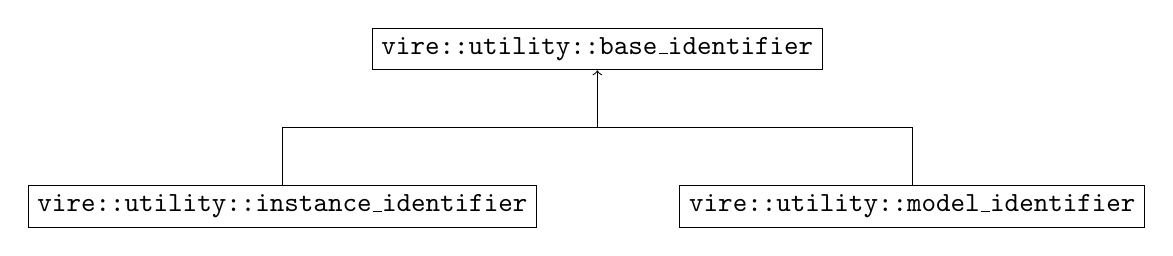
\begin{tikzpicture}
  \node (base)  at (0,2)  [draw] {\texttt{vire::utility::base\_identifier}};
  \node (instance)  at (-4,0) [draw] {\texttt{vire::utility::instance\_identifier}};
  \node (model) at (4,0)  [draw] {\texttt{vire::utility::model\_identifier}};

  \draw (node cs:name=model,anchor=north) |- (0,1);
\draw[->] (node cs:name=instance,anchor=north)
  |- (0,1) -| (node cs:name=base,anchor=south);
\end{tikzpicture}
\end{center}

The          \texttt{vire::utility::base\_identifier}          (figure
\ref{fig-app-payload-base_identifier}) class is  a pure abstract class
that cannot be instantiated. However  it contains a mandatory name and
an  optional  version description  which  are  used by  all  inherited
classes:

\begin{itemize}

\item The   \texttt{vire::utility::instance\_identifier}    concrete   class
inherits  \texttt{vire::utility::base\_identifier}  and   is  used  to
identify \underline{unique instances of objects} known by the system.

\item The  \texttt{vire::utility::model\_identifier}   concrete  class  also
inherits  \texttt{vire::utility::base\_identifier}  and   is  used  to
identify \underline{types of objects} registered in the system.

\end{itemize}

The only difference between these two classes is the validation scheme
of  the name  attribute.

\begin{figure}[h]
\vskip 10pt
\small
\begin{Verbatim}[frame=single,xleftmargin=0.cm,label=\fbox{C++}]
struct base_identifier
{
  // Attributes:
  std::string name;    // The mandatory name uniquely identifying the object or
                       // the type of object.
  std::string version; // An optional character string representing the version
                       // of the object type.
};
\end{Verbatim}
\normalsize
\caption{The structure of the \texttt{vire::utility::base\_identifier}
  class (C++).}
\label{fig-app-payload-base_identifier}
\end{figure}

%%  Figure  \ref{fig-app-payload-identifier-json}
%% shows an example of instance indentifier.
%% \begin{figure}[h]
%% \vskip 10pt
%% \small
%% \begin{Verbatim}[frame=single,xleftmargin=0.cm,label=\fbox{\texttt{JSON}}]
%% {
%%   "name" : "vire::resource::invalid_resource_error",
%%   "version" : "1.0"
%% }
%% \end{Verbatim}
%% \normalsize
%% \caption{JSON  formatted class identifier  object (class
%%   \texttt{vire::utility::model\_identifier}).   Here one  identifies a
%%   specific error type.}
%% \label{fig-app-payload-identifier-json}
%% \end{figure}


\vfill
\pagebreak
\clearpage

\subsubsection{Resource related objects}

\begin{itemize}

\item
Class \texttt{vire::cms::invalid\_resource\_error} (figure \ref{fig-app-payload-invalid_resource_error}).

\begin{center}
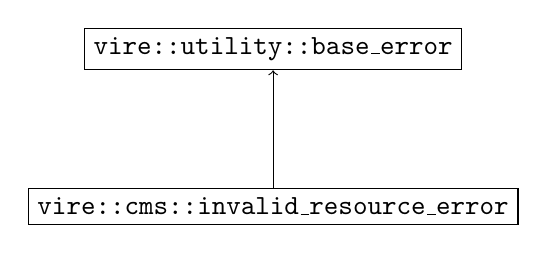
\begin{tikzpicture}
  \node (base)  at (0,2)  [draw] {\texttt{vire::utility::base\_error}};
  \node (ire)  at (0,0) [draw] {\texttt{vire::cms::invalid\_resource\_error}};
  \draw[->] (node cs:name=ire,anchor=north)
  |- (0,1) -| (node cs:name=base,anchor=south);
\end{tikzpicture}
\end{center}

\begin{figure}[h]
\vskip 10pt
\small
\begin{Verbatim}[frame=single,xleftmargin=0.cm,label=\fbox{C++}]
struct vire::cms::invalid_resource_error : public vire::utility::base_error
{
  // Attributes:
  std::string invalid_resource_path; // Invalid resource path
  std::string invalid_resource_id;   // Invalid resource internal ID (Vire server only)
};
\end{Verbatim}
\normalsize
\caption{The structure  of a invalid resource error object (C++).}
\label{fig-app-payload-invalid_resource_error}
\end{figure}

\begin{figure}[h]
\vskip 10pt
\small
\begin{Verbatim}[frame=single,xleftmargin=0.cm,label=\fbox{JSON++}]
{
  "code" : "3",
  "message_format" : "Resource path 'Atlas://Calorimeter/HV/Crate1/stop' is invalid",
  "invalid_resource_path" : "Atlas://Calorimeter/HV/Crate1/stop"
}
\end{Verbatim}
\normalsize
\caption{JSON formatted invalid resource error object.}
\label{fig-app-payload-invalid_resource_error-json}
\end{figure}


\item
Class     \texttt{vire::cms::resource\_status\_record}    (figure
\ref{fig-app-payload-resource_status_record}).

\end{itemize}

\begin{figure}[h]
\vskip 10pt
\small
\begin{Verbatim}[frame=single,xleftmargin=0.cm,label=\fbox{C++}]
struct vire::cms::resource_status_record
{
  // Attributes:
  std::string path;      // Path of the resource
  std::string timestamp; // Timestamp of the last modification
  uint16_t    flags;     // Status bits (Missing/Disabled/Pending/Error)
};
\end{Verbatim}
\normalsize
\caption{The structure  of a resource status record object (C++).}
\label{fig-app-payload-resource_status_record}
\end{figure}


\begin{figure}[h]
\vskip 10pt
\small
\begin{Verbatim}[frame=single,xleftmargin=0.cm,label=\fbox{JSON}]
{
  "path" : "SuperNEMO://Demonstrator/CMS/Coil/Control/Current/__dp_read__",
  "timestamp" : "20160612T212432.324517",
  "flags" : 2
}
\end{Verbatim}
\normalsize
\caption{JSON formatted resource status record object.}
\label{fig-app-payload-resource_status_record-json}
\end{figure}

\vfill
\pagebreak
\clearpage

\subsection{Connection of the Vire server to the CMS server}


\begin{itemize}

\item   The   \texttt{vire::cmslapp::connection\_request}   class
  (version \texttt{1.0})  represents a connection request  sent by the
  Vire server to the  CMS server through the \textcolor{blue}{service}
  channel.

\begin{center}
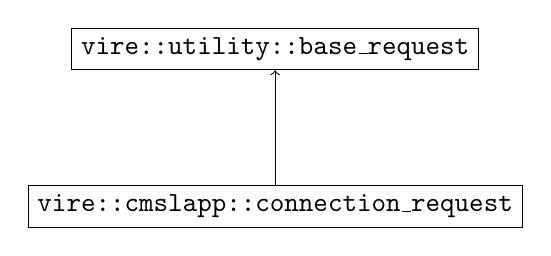
\begin{tikzpicture}
  \node (base)  at (0,2)  [draw] {\texttt{vire::utility::base\_request}};
  \node (cr)  at (0,0) [draw] {\texttt{vire::cmslapp::connection\_request}};
  \draw[->] (node cs:name=cr,anchor=north)
  |- (0,1) -| (node cs:name=base,anchor=south);
\end{tikzpicture}
\end{center}

\noindent Class registration:
\begin{itemize}
\item name: \texttt{"vire::cmslapp::connection\_request"}
\item version: "1.0"
\end{itemize}

\begin{figure}[h]
\vskip 10pt
\small
\begin{Verbatim}[frame=single,xleftmargin=0.cm,label=\fbox{C++}]
struct vire::cmslapp::connection_request : public vire::utility::base_request
{
  // Attributes:
  vire::utility::instance_identifier  setup_id; // Identifier of the experimental setup
  std::vector<std::string> requested_resources; // The list of requested resources
                                                // addressed by path
};
\end{Verbatim}
\normalsize
\caption{The structure of the connection  request object to be emitted
  by the Vire server to the CMS server (C++).}
\label{fig-app-payload-connection_request}
\end{figure}

\begin{figure}[h]
\vskip 10pt
\small
\begin{Verbatim}[frame=single,xleftmargin=0.cm,label=\fbox{JSON}]
{
  "setup_id" : {
    "name" : "snemo",
    "version" : "1.0.2"
  },
  "requested_resources" : [
    "SuperNEMO://Demonstrator/CMS/Coil/PS/Control/Current/__dp_read__",
    "SuperNEMO://Demonstrator/CMS/Coil/PS/Control/Current/__dp_write__",
    ...
    "SuperNEMO://Demonstrator/CMS/Acquisition/start",
    "SuperNEMO://Demonstrator/CMS/Acquisition/stop"
  ]
}
\end{Verbatim}
\normalsize
\caption{A JSON formatted  connection request object sent  by the Vire
  server to the CMS server (C++).}
\label{fig-app-payload-connection_request-json}
\end{figure}


\item  The  \texttt{vire::cmslapp::connection\_success\_response}
  class represents  the response sent back  to the Vire server  by the
  CMS server through the  \textcolor{blue}{service} channel in case of
  success.

\begin{center}
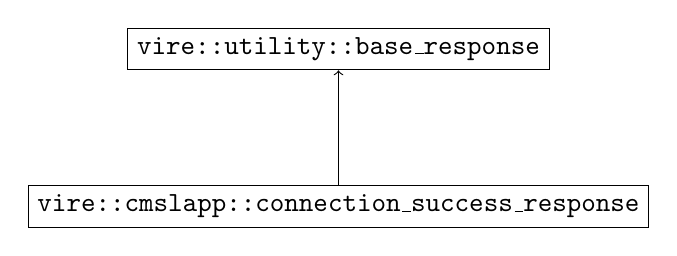
\begin{tikzpicture}
  \node (base)  at (0,2)  [draw] {\texttt{vire::utility::base\_response}};
  \node (csr)  at (0,0) [draw] {\texttt{vire::cmslapp::connection\_success\_response}};
  \draw[->] (node cs:name=csr,anchor=north)
  |- (0,1) -| (node cs:name=base,anchor=south);
\end{tikzpicture}
\end{center}

\noindent Class registration:
\begin{itemize}
\item name: \texttt{"vire::cmslapp::connection\_success\_response"}
\item version: "1.0"
\end{itemize}

\begin{figure}[h]
\vskip 10pt
\small
\begin{Verbatim}[frame=single,xleftmargin=0.cm,label=\fbox{C++}]
struct connection_success_response
  : public vire::utility::base_response
{
  typedef vire::resource::resource_status_record resource_status_record; // Type alias

  // Attributes:
  std::vector<resource_status_record> resources_snapshot; // Requested resources snapshot
};
\end{Verbatim}
\normalsize
\caption{The structure  of the connection success  response emitted by
  the CMS server to the Vire server (C++).}
\label{fig-app-payload-connection_success_response}
\end{figure}



\begin{figure}[h]
\vskip 10pt
\small
\begin{Verbatim}[frame=single,xleftmargin=0.cm,label=\fbox{\texttt{JSON}}]
{
  "resources_snapshot"  : [
    {
      "path" : "SuperNEMO://Demonstrator/CMS/Coil/PS/Control/Current/__dp_read__",
      "timestamp" : "20160612T212432.324517",
      "flags" : "0000"
    },
    {
      "path" : "SuperNEMO://Demonstrator/CMS/Coil/PS/Control/Current/__dp_write__",
      "timestamp" : "20160612T212432.328732",
      "flags" : "0000"
    },
    ...
    {
      "path" : "SuperNEMO://Demonstrator/CMS/Acquisition/start",
      "timestamp" : "20160612T212432.371671",
      "flags" : "0000"
    },
    {
      "path" : "SuperNEMO://Demonstrator/CMS/Acquisition/stop",
      "timestamp" : "20160612T212432.373624",
      "flags" : "0100"
    }
  ]
}
\end{Verbatim}
\normalsize
\caption[JSON formatted  connection success response]  {JSON formatted
  connection        success        response       object        (class
  \texttt{vire::cmslapp::connection\_success\_response}.}
\label{fig-app-payload-connection_success_response-json}
\end{figure}


\item
The  \texttt{vire::cmslapp::connection\_failure\_response}  class
represents the response sent back to the Vire server by the CMS server
through the \textcolor{blue}{service} channel in case of failure.

\begin{center}
\begin{tikzpicture}
  \node (base)  at (0,2)  [draw] {\texttt{vire::utility::base\_response}};
  \node (cfr)  at (0,0) [draw] {\texttt{vire::cmslapp::connection\_failure\_response}};
  \draw[->] (node cs:name=cfr,anchor=north)
  |- (0,1) -| (node cs:name=base,anchor=south);
\end{tikzpicture}
\end{center}

\begin{figure}[h]
\vskip 10pt
\small
\begin{Verbatim}[frame=single,xleftmargin=0.cm,label=\fbox{C++}]
struct connection_failure_response
  : public vire::utility::base_response
{
  // Nested type alias:
  typedef vire::utility::model_identifier error_identifier;

  // Nested error type aliases:
  typedef vire::utility::invalid_context_error invalid_context_error;
  typedef vire::utility::invalid_setup_id_error invalid_setup_id_error;

  // Nested error type:
  struct unknown_resources_error : public vire::utility::base_error {
    std::vector<std::string> unknown_paths; // List of unknown resources' paths
  };

  // Attributes:
  error_identifier error_id; // Error type identifier
  XXX_error        error;    // Embedded error record of one of the nested error type above
};
\end{Verbatim}
\normalsize
\caption{The structure  of the  connection failure response emitted
  by the CMS server to the Vire server (C++).}
\label{fig-app-payload-connection_failure_response}
\end{figure}


\end{itemize}

% \texttt{vire::cmsserver::disconnection\_request} (version \texttt{1.0})

\vfill
\pagebreak
\clearpage


\subsection{Disconnection of the Vire server from the CMS server}

\begin{itemize}

\item  The  \texttt{vire::cmslapp::disconnection\_request}  class
  represents a  disconnection request sent  by the Vire server  to the
  CMS server through the \textcolor{blue}{service} channel.

\begin{center}
\begin{tikzpicture}
  \node (base)  at (0,2)  [draw] {\texttt{vire::utility::base\_request}};
  \node (cr)  at (0,0) [draw] {\texttt{vire::cmslapp::disconnection\_request}};
  \draw[->] (node cs:name=cr,anchor=north)
  |- (0,1) -| (node cs:name=base,anchor=south);
\end{tikzpicture}
\end{center}

\noindent Class registration:
\begin{itemize}
\item name: \texttt{"vire::cmslapp::disconnection\_request"}
\item version: "1.0"
\end{itemize}

\begin{figure}[h]
\vskip 10pt
\small
\begin{Verbatim}[frame=single,xleftmargin=0.cm,label=\fbox{C++}]
struct disconnection_request : public vire::utility::base_request {
};
\end{Verbatim}
\normalsize
\caption{The structure of the disconnection  request object to be emitted
  by the Vire server to the CMS server (C++).}
\label{fig-app-payload-disconnection_request}
\end{figure}

%% \begin{figure}[h]
%% \vskip 10pt
%% \small
%% \begin{Verbatim}[frame=single,xleftmargin=0.cm,label=\fbox{C++}]
%% {
%% }
%% \end{Verbatim}
%% \normalsize
%% \caption{A JSON formatted  connection request object sent  by the Vire
%%   server to the CMS server (C++).}
%% \label{fig-app-payload-connection_request-json}
%% \end{figure}


\item  The  \texttt{vire::cmslapp::disconnection\_success\_response}
  class represents  the response sent back  to the Vire server  by the
  CMS server through the  \textcolor{blue}{service} channel in case of
  success.

\begin{center}
\begin{tikzpicture}
  \node (base)  at (0,2)  [draw] {\texttt{vire::utility::base\_response}};
  \node (csr)  at (0,0) [draw] {\texttt{vire::cmslapp::disconnection\_success\_response}};
  \draw[->] (node cs:name=csr,anchor=north)
  |- (0,1) -| (node cs:name=base,anchor=south);
\end{tikzpicture}
\end{center}


\noindent Class registration:
\begin{itemize}
\item name: \texttt{"vire::cmslapp::disconnection\_success\_response"}
\item version: "1.0"
\end{itemize}

\begin{figure}[h]
\vskip 10pt
\small
\begin{Verbatim}[frame=single,xleftmargin=0.cm,label=\fbox{C++}]
struct disconnection_success_response
  : public vire::utility::base_response
{
};
\end{Verbatim}
\normalsize
\caption{The structure  of the disconnection success  response emitted by
  the CMS server to the Vire server (C++).}
\label{fig-app-payload-disconnection_success_response}
\end{figure}


\end{itemize}


\vfill
\pagebreak
\clearpage

\subsection{Resource related payload objects}

\subsubsection{Resource Pub/Sub service}

\begin{itemize}

\item  The \texttt{vire::resource::resource\_pubsub\_request} object is responsible of
  demanding the activation/deactivation of the Pub/Sub service associated to a given
  resource (fig. \ref{fig-app-payload-resource_pubsub_request}).

\begin{figure}[h]
\vskip 10pt
\small
\begin{Verbatim}[frame=single,xleftmargin=0.cm,label=\fbox{C++}]
struct resource_pubsub_request
  : public vire::utility::base_request
{
  // Attributes:
  std::string path;      // The resource path.
  bool        subscribe; // Pub/Sub service (un)subscribe flag.
};
\end{Verbatim}
\normalsize
\caption{The structure of the \texttt{vire::resource::resource\_pubsub\_request}
  class (C++).}
\label{fig-app-payload-resource_pubsub_request}
\end{figure}

\item The \texttt{vire::resource::resource\_pubsub\_success\_response}
  object encapsulate a  successfull response of the CMS  server to the
  Vire  server  concerning   the  subscription/unsubscription  of  the
  Pub/Sub     service    associated     to     a    given     resource
  (fig. \ref{fig-app-payload-resource_pubsub_success_response}).

\begin{figure}[h]
\vskip 10pt
\small
\begin{Verbatim}[frame=single,xleftmargin=0.cm,label=\fbox{C++}]
struct resource_pubsub_success_response
  : public vire::utility::base_response
{
  // Pub/Sub mechanism type alias:
  typedef vire::resource::amqp_mechanism_address amqp_mechanism_address;

  // Type alias:
  typedef vire::utility::model_identifier pubsub_mechanism_identifier;
  typedef boost::variant<
      amqp_mechanism_address
      > pubsub_address_type;

  // Attributes:
  std::string                 path;               // The resource path.
  bool                        subscribe;          // The effective (un)subscribe flag.
  pubsub_mechanism_identifier pubsub_mechanism_id; // The mechanism for accessing Pub/Sub service
  pubsub_address_type         pubsub_address;      // If activation is set, this describes the
                                                   // access to the Pub/Sub service.
};
\end{Verbatim}
\normalsize
\caption{The structure of the \texttt{vire::resource::resource\_pubsub\_success\_response}
  class (C++).}
\label{fig-app-payload-resource_pubsub_success_response}
\end{figure}

\small
\begin{Verbatim}[frame=single,xleftmargin=0.cm,label=\fbox{JSON++}]
{
  "path" : "SuperNEMO://Demonstrator/CMS/Coil/PS/Monitoring/__dp_read__",
  "subscribe" : "true",
  "pubsub_mechanism_id" : "vire::amqp",
  "pubsub_address" : {
     "server" : "snemo.amqp",
     "port" : 1234,
     "channel" : "snemo.amqp.cms.pubsub.WAqq7ERzs1",
     "binding" : "SuperNEMO://Demonstrator/CMS/Coil/PS/Monitoring/__dp_read__",
     "key" : "coil.monitoring.pubsub"
  }
}
\end{Verbatim}
\normalsize

\item    The   \texttt{vire::resource::amqp\_mechanism\_address}    object
  describes   the  access   to   Pub/Sub   service  through   RabbitMQ
  (fig. \ref{fig-app-payload-amqp_pubsub_access_type}).

\begin{figure}[h]
\vskip 10pt
\small
\begin{Verbatim}[frame=single,xleftmargin=0.cm,label=\fbox{C++}]
struct amqp_mechanism_address
{
  // Attributes:
  std::string server;  // The AMQP server
  int         port;    // The AMQP server port
  std::string channel; // The RabbitMQ Pub/Sub channel.
  std::string binding; // The binding dedicated to this Pub/Sub service.
  std::string key;     // The Pub/Sub specific key/topic.
};
\end{Verbatim}
\normalsize
\caption{The structure of the \texttt{vire::resource::amqp\_pubsub\_access\_type}
  class (C++).}
\label{fig-app-payload-amqp_pubsub_access_type}
\end{figure}


\item The \texttt{vire::resource::resource\_pubsub\_failure\_response}
  object describes a failure response  concerning a request on Pub/Sub
  service       associated       to       a       given       resource
  (fig. \ref{fig-app-payload-resource_pubsub_failure_response}).


\begin{figure}[h]
\vskip 10pt
\small
\begin{Verbatim}[frame=single,xleftmargin=0.cm,label=\fbox{C++}]
struct resource_pubsub_failure_response
  : public vire::utility::base_response
{
  // Nested type alias:
  typedef vire::utility::model_identifier error_type_identifier;

  // Nested error type aliases:
  typedef vire::utility::invalid_context_error  invalid_context_error;
  typedef vire::utility::invalid_resource_error invalid_resource_error;

  // Nested error type:
  struct no_pubsub_resource_error : public vire::utility::base_error {
    std::string path; // The path of the resource without Pub/Sub service support
  };

  typedef boost::variant<
     invalid_context_error,
     invalid_resource_error,
     no_pubsub_resource_error
     > error_type;

  // Attributes:
  error_type_identifier error_type_id; // Error type identifier.
  error_type            error;        // Embedded error record of one of
                                      // the nested error types above.
};
\end{Verbatim}
\normalsize
\caption{The structure of the \texttt{vire::resource::resource\_pubsub\_failure\_response}
  class (C++).}
\label{fig-app-payload-resource_pubsub_failure_response}
\end{figure}

\end{itemize}

\vfill
\pagebreak
\clearpage

\subsubsection{Fetching resource status}

\begin{center}
\begin{tikzpicture}
  \node (payload)  at (0,2) [draw] {\texttt{vire::utility::base\_request}};
  \node (request)  at (0,0) [draw] {\texttt{vire::resource::resource\_fetch\_status\_request}};
  \draw[->] (node cs:name=request,anchor=north)
  |- (0,1) -| (node cs:name=payload,anchor=south);
\end{tikzpicture}
\end{center}

\begin{itemize}

\item The \texttt{vire::resource::resource\_fetch\_status\_request} object
  demands to the CMS server an updated status record associated to a given resource
(fig. \ref{fig-app-payload-resource_fetch_status_request}).

\begin{figure}[h]
\vskip 10pt
\small
\begin{Verbatim}[frame=single,xleftmargin=0.cm,label=\fbox{C++}]
struct resource_fetch_status_request
  : public vire::utility::base_request
{
  // Attributes:
  std::string path; // Resource path.
};
\end{Verbatim}
\normalsize
\caption{The structure of a \texttt{vire::utility::resource\_fetch\_status\_request} object
  (C++).}
\label{fig-app-payload-resource_fetch_status_request}
\end{figure}

\item The \texttt{vire::resource::resource\_fetch\_status\_success\_response} object
  transmits the updated/current status record  associated to a given resource
(fig. \ref{fig-app-payload-resource_fetch_status_success_response}).

\begin{figure}[h]
\vskip 10pt
\small
\begin{Verbatim}[frame=single,xleftmargin=0.cm,label=\fbox{C++}]
struct resource_fetch_status_success_response
  : public vire::utility::base_response
{
  // Nested type alias:
  typedef vire::resource::resource_status_record resource_status_record;

  // Attributes:
  resource_status_record status; // The resource status record.
};
\end{Verbatim}
\normalsize
\caption{The structure of a \texttt{vire::utility::resource\_fetch\_status\_success\_response} object
  (C++).}
\label{fig-app-payload-resource_fetch_status_success_response}
\end{figure}



\item The \texttt{vire::resource::resource\_fetch\_status\_failure\_response} object
  describes a failure detected by the CMS server in response to a resource fetch status request.

\begin{figure}[h]
\vskip 10pt
\small
\begin{Verbatim}[frame=single,xleftmargin=0.cm,label=\fbox{C++}]
struct resource_fetch_status_failure_response
  : public vire::utility::base_response
{
  // Nested type alias:
  typedef vire::utility::model_identifier error_identifier;

  // Nested error type aliases:
  typedef vire::utility::invalid_context_error   invalid_context_error;
  typedef vire::resource::invalid_resource_error invalid_resource_error;

  // Attributes:
  error_identifier error_id; // Error type identifier
  XXX_error        error;    // Embedded error record of one of the nested error type above
};
\end{Verbatim}
\normalsize
\caption{The structure of a \texttt{vire::utility::resource\_fetch\_status\_failure\_response} object
  (C++).}
\label{fig-app-payload-resource_fetch_status_failure_response}
\end{figure}


\end{itemize}


\vfill
\pagebreak
\clearpage

\subsubsection{Synchronous/blocking resource execution}

\begin{center}
\begin{tikzpicture}
  \node (payload)  at (0,2)   [draw] {\texttt{vire::utility::base\_request}};
  \node (request)  at (0,0)  [draw] {\texttt{vire::resource::resource\_exec\_request}};
  \draw[->] (node cs:name=request,anchor=north)
  |- (0,1) -| (node cs:name=payload,anchor=south);
\end{tikzpicture}
\end{center}

\begin{itemize}

\item The \texttt{vire::resource::resource\_exec\_request} object represent a resource execution request
in blocking (synchronous) mode.


\begin{figure}[h]
\vskip 10pt
\small
\begin{Verbatim}[frame=single,xleftmargin=0.cm,label=\fbox{C++}]
struct resource_exec_request
  : public vire::utility::base_request
{
  // Type alias:
  typedef vire::resource::method_argument method_argument;

  // Attributes:
  std::string                  path;            // Resource path.
  std::vector<method_argument> input_arguments; // Embedded error record of one of
                                                // the nested error type above.
};
\end{Verbatim}
\normalsize
\caption{The structure of a \texttt{vire::utility::resource\_fetch\_status\_failure\_response} object
  (C++).}
\label{fig-app-payload-resource_fetch_status_failure_response}
\end{figure}

\item \texttt{vire::resource::resource\_exec\_success\_response}

\small
\begin{Verbatim}[frame=single,xleftmargin=0.cm,label=\fbox{C++}]
struct resource_exec_success_response
 : vire::utility::base_response
{
  // Type alias:
  typedef vire::resource::method_argument        method_argument;
  typedef vire::resource::resource_status_record resource_status_record;

  // Attributes:
  resource_status_record       status;               // Resource status
  std::string                  reception_timestamp;  // Request reception timestamp
  std::string                  completion_timestamp; // Execution completion timestamp
  std::vector<method_argument> output_arguments;     // Output arguments
};
\end{Verbatim}



\item \texttt{vire::resource::resource\_exec\_failure\_response}


\small
\begin{Verbatim}[frame=single,xleftmargin=0.cm,label=\fbox{C++}]
struct resource_exec_failure_response
 : vire::utility::base_response
{

  // Error type aliases:
  typedef vire::utility::invalid_context_error   invalid_context_error;
  typedef vire::resource::invalid_resource_error invalid_resource_error;
  typedef vire::resource::invalid_status_error   invalid_status_error;
  typedef vire::resource::resource_exec_error    resource_exec_error;

  // Type aliases:
  typedef vire::utility::model_identifier        error_type_identifier;
  typedef boost::variant<
      invalid_context_error,
      invalid_resource_error,
      invalid_status_error,
      resource_exec_error> error_type;

  // Attributes:
  error_type_identifier error_type_id; // Error type identifier
  error_type            error;        // Embedded error record

};
\end{Verbatim}

\end{itemize}


\vfill
\pagebreak
\clearpage

\subsubsection{Asynchronous/non-blocking resource execution}

\begin{center}
\begin{tikzpicture}
  \node (payload)  at (0,2)   [draw] {\texttt{vire::utility::base\_request}};
  \node (request_nb)  at (0,0)  [draw] {\texttt{vire::resource::resource\_exec\_non\_blocking\_request}};
  \draw[->] (node cs:name=request_nb,anchor=north)
  |- (0,1) -| (node cs:name=payload,anchor=south);
\end{tikzpicture}
\end{center}

\begin{itemize}

\item \texttt{vire::resource::resource\_exec\_non\_blocking\_request}
\small
\begin{Verbatim}[frame=single,xleftmargin=0.cm,label=\fbox{C++}]
struct resource_exec_non_blocking_request
  : public vire::utility::base_request
{
  // Type alias:
  typedef vire::resource::method_argument method_argument;

  // Attributes:
  std::string                  path;            // Resource path.
  std::vector<method_argument> input_arguments; // Embedded error record of one of
                                                // the nested error type above.

};
\end{Verbatim}

\item \texttt{vire::resource::resource\_exec\_non\_blocking\_ack\_response}


\small
\begin{Verbatim}[frame=single,xleftmargin=0.cm,label=\fbox{C++}]
struct resource_exec_non_blocking_ack_response
 : vire::utility::base_response
{
  // Type alias:
  typedef vire::resource::method_argument        method_argument;
  typedef vire::resource::resource_status_record resource_status_record;

  // Attributes:
  resource_status_record       status;
  std::string                  reception_timestamp;

};
\end{Verbatim}


\item \texttt{vire::resource::resource\_exec\_non\_blocking\_noack\_response}


\small
\begin{Verbatim}[frame=single,xleftmargin=0.cm,label=\fbox{C++}]
struct resource_exec_non_blocking_noack_response
  : vire::utility::base_response
{
  // Type alias:
  typedef vire::resource::resource_status_record resource_status_record;
  typedef vire::utility::model_identifier error_type_identifier;

  // Error type aliases:
  typedef vire::utility::invalid_context_error   invalid_context_error;
  typedef vire::resource::invalid_resource_error invalid_resource_error;
  typedef vire::resource::invalid_status_error   invalid_status_error;
  typedef vire::resource::resource_exec_error    resource_exec_error;

  // Nested error type:
  struct no_non_blocking_exec_resource_error : public vire::utility::base_error {
    std::string path; // The path of the resource without non-blocking execution support
  };

  typedef boost::variant<
     invalid_context_error,
     invalid_resource_error,
     invalid_status_error,
     no_non_blocking_exec_resource_error,
     resource_exec_error
     > error_type;

  // Attributes:
  resource_status_record status;        // Resource status.
  error_type_identifier  error_type_id; // Error type identifier.
  error_type             error;         // Embedded error record of one of
                                        // the nested error types above.

};
\end{Verbatim}
\normalsize


\item \texttt{vire::resource::resource\_exec\_non\_blocking\_success\_event}


\small
\begin{Verbatim}[frame=single,xleftmargin=0.cm,label=\fbox{C++}]
struct resource_exec_non_blocking_success\_event
  : vire::utility::base_event
{
  // Type alias:
  typedef vire::resource::method_argument        method_argument;
  typedef vire::resource::resource_status_record resource_status_record;

  // Attributes:
  resource_status_record       status;               // Resource status
  std::string                  reception_timestamp;  // Request reception timestamp
  std::string                  completion_timestamp; // Execution completion timestamp
  std::vector<method_argument> output_arguments;     // Output arguments

};
\end{Verbatim}
\normalsize

\item \texttt{vire::resource::resource\_exec\_non\_blocking\_failure\_event}


\small
\begin{Verbatim}[frame=single,xleftmargin=0.cm,label=\fbox{C++}]
struct resource_exec_non_blocking_failure\_event
  : vire::utility::base_event
{

  // Error type aliases:
  typedef vire::utility::invalid_context_error   invalid_context_error;
  typedef vire::cms::invalid_resource_error invalid_resource_error;
  typedef vire::cms::invalid_status_error   invalid_status_error;
  typedef vire::cms::resource_exec_error    resource_exec_error;

  // Type aliases:
  typedef vire::utility::model_identifier        error_type_identifier;
  typedef boost::variant<
      vire::utility::invalid_context_error,
      vire::cms::invalid_resource_error,
      vire::cms::invalid_status_error,
      vire::cms::resource_exec_error> error_type;

  // Attributes:
  error_type_identifier error_type_id; // Error type identifier
  error_type            error;        // Embedded error record

};
\end{Verbatim}
\normalsize


\end{itemize}


\vfill
\pagebreak
\clearpage

% end


\section{The RabbitMQ based RPC system}\label{app:rabbitmq_rpc}

\subsection{Introduction}


\end{document}
%%

\vfill
\pagebreak
\clearpage

\documentclass[a4paper,11pt,twoside]{article}

%%% packages:
\usepackage[T1]{fontenc}
\usepackage{ucs}
\usepackage[utf8x]{inputenc}
%\usepackage[frenchb]{babel}
\usepackage{amsmath}
\usepackage{amssymb}
\usepackage{latexsym}
\usepackage{verbatim}
\usepackage{moreverb}
\usepackage{fancyvrb}
\usepackage{alltt}
\usepackage{eurosym}
\usepackage{hyperref}
\usepackage{colortbl}
\usepackage{graphicx}
\usepackage{pdflscape}
\usepackage{afterpage}
\usepackage{rotating}
\usepackage{tikz}
%\usepackage{tikz-qtree}

%%% Geometry (https://en.wikibooks.org/wiki/LaTeX/Page_Layout)
\usepackage{layout}
%\usepackage[a4paper,top=1in, bottom=1.25in, left=1.25in, right=1.25in, inner=4cm,outer=2cm]{geometry}
\usepackage[a4paper,inner=2cm,outer=2cm]{geometry}
%% \setlength{\hoffset}{-1inch}
%% \setlength{\voffset}{-1inch0pt}
\setlength{\textheight}{23cm}
%% \setlength{\textwidth}{18cm}

%%% macros:
\newcommand{\thepath}{.}
\newcommand{\imgpath}{\thepath/images}
\newcommand{\pdfteximgpath}{\thepath/pdftex}
\newcommand{\pdftextimgpath}{\thepath/pdftex_t}

%%%
\title{The SuperNEMO Vire-CMS/LAPP interface\\version 0.7}
\author{E.Chabanne, J.Hommet, T. Leflour, Y. Lemière,
  S.Lieunard, F.Mauger, J.-L. Panazol, J.Poincheval}
\date{\today}

%%%
\begin{document}

\thispagestyle{empty}
%\layout{}
\maketitle
\begin{abstract}
This document aims  to describe the requirements of  the Vire CMS/LAPP
interface,  i.e. the  software bridge  between the  Vire based  online
software  (Vire server  and clients,  a.k.a the  Vire system)  and the
CMS/LAPP server  that plays  the role  of the  unique gate  (subcontractor proxy) to
communicate with  the OPCUA-based MOS  servers responsible of  the low
level control and monitoring operations on some hardware devices.
\end{abstract}
\vfill
\pagebreak

\tableofcontents
\vfill
\pagebreak

\listoffigures
\vfill
\pagebreak

\listoftables
\vfill
\pagebreak
\clearpage

\documentclass[a4paper,11pt,twoside]{article}

%%% packages:
\usepackage[T1]{fontenc}
\usepackage{ucs}
\usepackage[utf8x]{inputenc}
%\usepackage[frenchb]{babel}
\usepackage{amsmath}
\usepackage{amssymb}
\usepackage{latexsym}
\usepackage{verbatim}
\usepackage{moreverb}
\usepackage{fancyvrb}
\usepackage{alltt}
\usepackage{eurosym}
\usepackage{hyperref}
\usepackage{colortbl}
\usepackage{graphicx}
\usepackage{pdflscape}
\usepackage{afterpage}
\usepackage{rotating}
\usepackage{tikz}
%\usepackage{tikz-qtree}

%%% Geometry (https://en.wikibooks.org/wiki/LaTeX/Page_Layout)
\usepackage{layout}
%\usepackage[a4paper,top=1in, bottom=1.25in, left=1.25in, right=1.25in, inner=4cm,outer=2cm]{geometry}
\usepackage[a4paper,inner=2cm,outer=2cm]{geometry}
%% \setlength{\hoffset}{-1inch}
%% \setlength{\voffset}{-1inch0pt}
\setlength{\textheight}{23cm}
%% \setlength{\textwidth}{18cm}

%%% macros:
\newcommand{\thepath}{.}
\newcommand{\imgpath}{\thepath/images}
\newcommand{\pdfteximgpath}{\thepath/pdftex}
\newcommand{\pdftextimgpath}{\thepath/pdftex_t}

%%%
\title{The SuperNEMO Vire-CMS/LAPP interface\\version 0.7}
\author{E.Chabanne, J.Hommet, T. Leflour, Y. Lemière,
  S.Lieunard, F.Mauger, J.-L. Panazol, J.Poincheval}
\date{\today}

%%%
\begin{document}

\thispagestyle{empty}
%\layout{}
\maketitle
\begin{abstract}
This document aims  to describe the requirements of  the Vire CMS/LAPP
interface,  i.e. the  software bridge  between the  Vire based  online
software  (Vire server  and clients,  a.k.a the  Vire system)  and the
CMS/LAPP server  that plays  the role  of the  unique gate  (subcontractor proxy) to
communicate with  the OPCUA-based MOS  servers responsible of  the low
level control and monitoring operations on some hardware devices.
\end{abstract}
\vfill
\pagebreak

\tableofcontents
\vfill
\pagebreak

\listoffigures
\vfill
\pagebreak

\listoftables
\vfill
\pagebreak
\clearpage

\documentclass[a4paper,11pt,twoside]{article}

%%% packages:
\usepackage[T1]{fontenc}
\usepackage{ucs}
\usepackage[utf8x]{inputenc}
%\usepackage[frenchb]{babel}
\usepackage{amsmath}
\usepackage{amssymb}
\usepackage{latexsym}
\usepackage{verbatim}
\usepackage{moreverb}
\usepackage{fancyvrb}
\usepackage{alltt}
\usepackage{eurosym}
\usepackage{hyperref}
\usepackage{colortbl}
\usepackage{graphicx}
\usepackage{pdflscape}
\usepackage{afterpage}
\usepackage{rotating}
\usepackage{tikz}
%\usepackage{tikz-qtree}

%%% Geometry (https://en.wikibooks.org/wiki/LaTeX/Page_Layout)
\usepackage{layout}
%\usepackage[a4paper,top=1in, bottom=1.25in, left=1.25in, right=1.25in, inner=4cm,outer=2cm]{geometry}
\usepackage[a4paper,inner=2cm,outer=2cm]{geometry}
%% \setlength{\hoffset}{-1inch}
%% \setlength{\voffset}{-1inch0pt}
\setlength{\textheight}{23cm}
%% \setlength{\textwidth}{18cm}

%%% macros:
\newcommand{\thepath}{.}
\newcommand{\imgpath}{\thepath/images}
\newcommand{\pdfteximgpath}{\thepath/pdftex}
\newcommand{\pdftextimgpath}{\thepath/pdftex_t}

%%%
\title{The SuperNEMO Vire-CMS/LAPP interface\\version 0.7}
\author{E.Chabanne, J.Hommet, T. Leflour, Y. Lemière,
  S.Lieunard, F.Mauger, J.-L. Panazol, J.Poincheval}
\date{\today}

%%%
\begin{document}

\thispagestyle{empty}
%\layout{}
\maketitle
\begin{abstract}
This document aims  to describe the requirements of  the Vire CMS/LAPP
interface,  i.e. the  software bridge  between the  Vire based  online
software  (Vire server  and clients,  a.k.a the  Vire system)  and the
CMS/LAPP server  that plays  the role  of the  unique gate  (subcontractor proxy) to
communicate with  the OPCUA-based MOS  servers responsible of  the low
level control and monitoring operations on some hardware devices.
\end{abstract}
\vfill
\pagebreak

\tableofcontents
\vfill
\pagebreak

\listoffigures
\vfill
\pagebreak

\listoftables
\vfill
\pagebreak
\clearpage

\input{cms_server/main.tex}
\vfill
\pagebreak
\clearpage

\input{vire_resources/main.tex}
\vfill
\pagebreak
\clearpage

% \input{cmslapp_vireclients/main.tex}
\section{Interaction of the CMS/LAPP server with Vire clients}

TODO
\vfill
\pagebreak
\clearpage

%%%%%%%%%
\appendix

\input{appendix/app_filesystem.tex}
\input{appendix/app_new_device.tex}
\input{appendix/app_vire_messages.tex}
%\input{appendix/app_json_fmt.tex}
\input{appendix/app_protobuf_format.tex}
\input{appendix/app_payload_objects.tex}
\input{appendix/app_rabbitmq_rpc.tex}

\end{document}
%%

\vfill
\pagebreak
\clearpage

\documentclass[a4paper,11pt,twoside]{article}

%%% packages:
\usepackage[T1]{fontenc}
\usepackage{ucs}
\usepackage[utf8x]{inputenc}
%\usepackage[frenchb]{babel}
\usepackage{amsmath}
\usepackage{amssymb}
\usepackage{latexsym}
\usepackage{verbatim}
\usepackage{moreverb}
\usepackage{fancyvrb}
\usepackage{alltt}
\usepackage{eurosym}
\usepackage{hyperref}
\usepackage{colortbl}
\usepackage{graphicx}
\usepackage{pdflscape}
\usepackage{afterpage}
\usepackage{rotating}
\usepackage{tikz}
%\usepackage{tikz-qtree}

%%% Geometry (https://en.wikibooks.org/wiki/LaTeX/Page_Layout)
\usepackage{layout}
%\usepackage[a4paper,top=1in, bottom=1.25in, left=1.25in, right=1.25in, inner=4cm,outer=2cm]{geometry}
\usepackage[a4paper,inner=2cm,outer=2cm]{geometry}
%% \setlength{\hoffset}{-1inch}
%% \setlength{\voffset}{-1inch0pt}
\setlength{\textheight}{23cm}
%% \setlength{\textwidth}{18cm}

%%% macros:
\newcommand{\thepath}{.}
\newcommand{\imgpath}{\thepath/images}
\newcommand{\pdfteximgpath}{\thepath/pdftex}
\newcommand{\pdftextimgpath}{\thepath/pdftex_t}

%%%
\title{The SuperNEMO Vire-CMS/LAPP interface\\version 0.7}
\author{E.Chabanne, J.Hommet, T. Leflour, Y. Lemière,
  S.Lieunard, F.Mauger, J.-L. Panazol, J.Poincheval}
\date{\today}

%%%
\begin{document}

\thispagestyle{empty}
%\layout{}
\maketitle
\begin{abstract}
This document aims  to describe the requirements of  the Vire CMS/LAPP
interface,  i.e. the  software bridge  between the  Vire based  online
software  (Vire server  and clients,  a.k.a the  Vire system)  and the
CMS/LAPP server  that plays  the role  of the  unique gate  (subcontractor proxy) to
communicate with  the OPCUA-based MOS  servers responsible of  the low
level control and monitoring operations on some hardware devices.
\end{abstract}
\vfill
\pagebreak

\tableofcontents
\vfill
\pagebreak

\listoffigures
\vfill
\pagebreak

\listoftables
\vfill
\pagebreak
\clearpage

\input{cms_server/main.tex}
\vfill
\pagebreak
\clearpage

\input{vire_resources/main.tex}
\vfill
\pagebreak
\clearpage

% \input{cmslapp_vireclients/main.tex}
\section{Interaction of the CMS/LAPP server with Vire clients}

TODO
\vfill
\pagebreak
\clearpage

%%%%%%%%%
\appendix

\input{appendix/app_filesystem.tex}
\input{appendix/app_new_device.tex}
\input{appendix/app_vire_messages.tex}
%\input{appendix/app_json_fmt.tex}
\input{appendix/app_protobuf_format.tex}
\input{appendix/app_payload_objects.tex}
\input{appendix/app_rabbitmq_rpc.tex}

\end{document}
%%

\vfill
\pagebreak
\clearpage

% \documentclass[a4paper,11pt,twoside]{article}

%%% packages:
\usepackage[T1]{fontenc}
\usepackage{ucs}
\usepackage[utf8x]{inputenc}
%\usepackage[frenchb]{babel}
\usepackage{amsmath}
\usepackage{amssymb}
\usepackage{latexsym}
\usepackage{verbatim}
\usepackage{moreverb}
\usepackage{fancyvrb}
\usepackage{alltt}
\usepackage{eurosym}
\usepackage{hyperref}
\usepackage{colortbl}
\usepackage{graphicx}
\usepackage{pdflscape}
\usepackage{afterpage}
\usepackage{rotating}
\usepackage{tikz}
%\usepackage{tikz-qtree}

%%% Geometry (https://en.wikibooks.org/wiki/LaTeX/Page_Layout)
\usepackage{layout}
%\usepackage[a4paper,top=1in, bottom=1.25in, left=1.25in, right=1.25in, inner=4cm,outer=2cm]{geometry}
\usepackage[a4paper,inner=2cm,outer=2cm]{geometry}
%% \setlength{\hoffset}{-1inch}
%% \setlength{\voffset}{-1inch0pt}
\setlength{\textheight}{23cm}
%% \setlength{\textwidth}{18cm}

%%% macros:
\newcommand{\thepath}{.}
\newcommand{\imgpath}{\thepath/images}
\newcommand{\pdfteximgpath}{\thepath/pdftex}
\newcommand{\pdftextimgpath}{\thepath/pdftex_t}

%%%
\title{The SuperNEMO Vire-CMS/LAPP interface\\version 0.7}
\author{E.Chabanne, J.Hommet, T. Leflour, Y. Lemière,
  S.Lieunard, F.Mauger, J.-L. Panazol, J.Poincheval}
\date{\today}

%%%
\begin{document}

\thispagestyle{empty}
%\layout{}
\maketitle
\begin{abstract}
This document aims  to describe the requirements of  the Vire CMS/LAPP
interface,  i.e. the  software bridge  between the  Vire based  online
software  (Vire server  and clients,  a.k.a the  Vire system)  and the
CMS/LAPP server  that plays  the role  of the  unique gate  (subcontractor proxy) to
communicate with  the OPCUA-based MOS  servers responsible of  the low
level control and monitoring operations on some hardware devices.
\end{abstract}
\vfill
\pagebreak

\tableofcontents
\vfill
\pagebreak

\listoffigures
\vfill
\pagebreak

\listoftables
\vfill
\pagebreak
\clearpage

\input{cms_server/main.tex}
\vfill
\pagebreak
\clearpage

\input{vire_resources/main.tex}
\vfill
\pagebreak
\clearpage

% \input{cmslapp_vireclients/main.tex}
\section{Interaction of the CMS/LAPP server with Vire clients}

TODO
\vfill
\pagebreak
\clearpage

%%%%%%%%%
\appendix

\input{appendix/app_filesystem.tex}
\input{appendix/app_new_device.tex}
\input{appendix/app_vire_messages.tex}
%\input{appendix/app_json_fmt.tex}
\input{appendix/app_protobuf_format.tex}
\input{appendix/app_payload_objects.tex}
\input{appendix/app_rabbitmq_rpc.tex}

\end{document}
%%

\section{Interaction of the CMS/LAPP server with Vire clients}

TODO
\vfill
\pagebreak
\clearpage

%%%%%%%%%
\appendix


\section{Filesystem and configuration files management}\label{app:filesystem_conf}

Let's consider  a simple  situation where  one runs  the Vire  and CMS
software  tools (servers)  on a  single Linux  machine (the  CMS host)
under            the            \texttt{"nemoprod"}            generic
account\footnote{\texttt{"nemoprod"}  is  the   login  of  th  generic
  account used at the CCIN2P3  cluster to perform automated management
  operations on experimental and  Monte-Carlo data file: data transfer
  from LSM or LSC labs to CCIN2P3, calibration and reconstruction data
  processing, storage on HPPS.}.

\begin{itemize}
\item Hostname login : \verb|192.168.1.10| (private IP) %\texttt{snemocms.lsm.in2p3.fr} (public address)
\item User login : \texttt{nemoprod}
\item Main group : \texttt{supernemo}
\item Home directory : \verb|/home/nemoprod| (a.k.a. \verb|~nemoprod|)
\end{itemize}

\noindent  We  assume that  the  SuperNEMO  online software  has  been
installed   and  setup   in  the   home  directory,   for  example in
\verb|/home/nemoprod/Private/Software/| :
\vskip 20pt
\small
\begin{Verbatim}[frame=single,xleftmargin=0.cm,label=\fbox{Filesystem}]
/home/nemoprod/Private/Software
|-- Cadfael/ # base directory of the Cadfael software framework
|-- Bayeux/  # base directory of the Bayeux software framework
|-- Vire/    # base directory of the Vire software framework
|-- OPCUA/   # base directory of the OPCUA+MOS software framework
`-- Falaise/ # base directory of the Falaise software framework
\end{Verbatim}
\normalsize

\noindent  We consider  here  that the  Falaise  library package  will
contain  the mandatory  configuration files  that describe  the online
software, both for the Vire and CMS/MOS parts:
\vskip 20pt
\small
\begin{Verbatim}[frame=single,xleftmargin=0.cm,label=\fbox{Filesystem}]
/home/nemoprod/Private/Software
:
`-- Falaise/
    :
    `-- Install/
        `-- Falaise-3.0.0/
            |-- bin/
            |   :
            |   |-- flquery
            |   |-- flreconstruct
            |   `-- flsimulate
            |-- include/
            :   :
            |-- lib/
            |   `-- x86_64-linux-gnu/
            |       :
            |       |-- libFalaise.so
            |       :
            `-- share/
                `-- Falaise-3.0.0/
                    `-- resources/
                        `-- config/
                            `-- online/
                                :
                                :
\end{Verbatim}
\normalsize

\noindent Where:
\begin{itemize}
\item                                                              the
  \verb|/home/nemoprod/Private/Software/Falaise/Install/Falaise-3.0.0|
  is  the  installation  prefix  of  the  Falaise  library  (binaries,
  includes) and associated resource files.
\item      the     \verb|share/Falaise-3.0.0/resources/config/online/|
  subdirectory  is the  tree  of configuration  files  that should  be
  accessible  by  any online  software  component  (Vire server,  Vire
  clients, CMS and MOS servers).
\end{itemize}


\noindent  Let's consider  the \verb|.../config/online/|  directory as
the base directory for all online configuration files for the Vire and
CMS  servers.   All  configuration  files  should  thus  be  addressed
relatively to this place.

\noindent  We  propose to  use  one  of  the following  techniques  to
represent this base directory:

\begin{itemize}
\item         a         dedicated         environment         variable
  \verb|SNEMO_ONLINE_CONFIG_BASE_DIR| recognized by  both Vire and CMS
  servers. It could be setup within the environment with:
\vskip 20pt
\small
\begin{Verbatim}[frame=single,xleftmargin=0.cm,label=\fbox{shell}]
export FALAISE_INSTALL_DIR=\
  ${HOME}/Private/Software/Falaise/Install/Falaise-3.0.0
export SNEMO_ONLINE_CONFIG_BASE_DIR=\
  ${FALAISE_INSTALL_DIR}/share/Falaise-3.0.0/resources/config/online
\end{Verbatim}
\normalsize

\item a  path registration label as  implemented in the kernel  of the
  Bayeux library:\\
  \noindent The \verb|@snonlinecfg:| label \\
  is associated to\\
  \noindent \hskip 50pt\verb|${FALAISE_INSTALL_DIR}/share/Falaise-3.0.0/resources/config/online|

\end{itemize}

\noindent Thus a specific  configuration file \verb|dummy.conf| could be
addressed with one of the following syntaxes:

\begin{itemize}

\item[(a)]
  \verb|${SNEMO_ONLINE_CONFIG_BASE_DIR}/snemo/1.0.2/dummy.conf|       :
  supported  by  Vire  and  CMS  using  word  expansion  utility  like
  \texttt{wordexp} (for C/C++ languages),

\item[(b)]  \verb|@snonlinecfg:snemo/1.0.2/dummy.conf|  : supported  by
  Vire  only  for  now,  thanks to  the  path  registration  mechanism
  implemented in the Bayeux API,

\item[(c)] \verb|snemo/1.0.2/dummy.conf| : can be supported by Vire and
  CMS  but  is  ambiguous  because  such a relative  path  can  be  also
  interpreted as a path relatively  to the current directory (\verb|./|)
  and not to the online configuration directory.

\end{itemize}

We suggests  the use  of an  explicit environment  variable as  in (a)
because it  is simple to  implement in various languages  and software
frameworks and should not imply any ambiguous file path resolution.

\vfill
\pagebreak
\clearpage

% end


\section{Integration of a new device}\label{app:new_device}

Both Vire  and MOS systems are  designed to be expandable  in terms of
device integration.  This section  decribes the  integration of  a new
device in the \emph{Control and Monitoring System}.

\subsection{Integration of a new device in the MOS environment}

Any new device is described through  a dedicated XML model file.  This
XML  file  is  created  from  a  template  file  elaborated  from  the
\emph{interface control document} (ICD) and associated to the model of
the  device. The  format  of the  XML  file is  described  in the  MOS
(Multipurpose OPCUA Server) User Guide. % ref

Typically, a device is embedded in a OPCUA server and implemented as a
OPCUA  \emph{simple  device}.   The  OPCUA server  itself  is  located
through an unique dedicated IP address and port.

The simple device  instance, hosted in the OPCUA  server, may contains
other sub-devices and/or \emph{datapoints}.   It is thus considered as
the root  of a hierarchy  of daughter  objects at deeper  levels.  The
daughter objects (devices or datapoints) are named relatively to their
top level  parent device. Figure  \ref{fig:an:mos_dev_1} shows an
example of a device embedded in a MOS server.

\begin{figure}[h]
\begin{center}
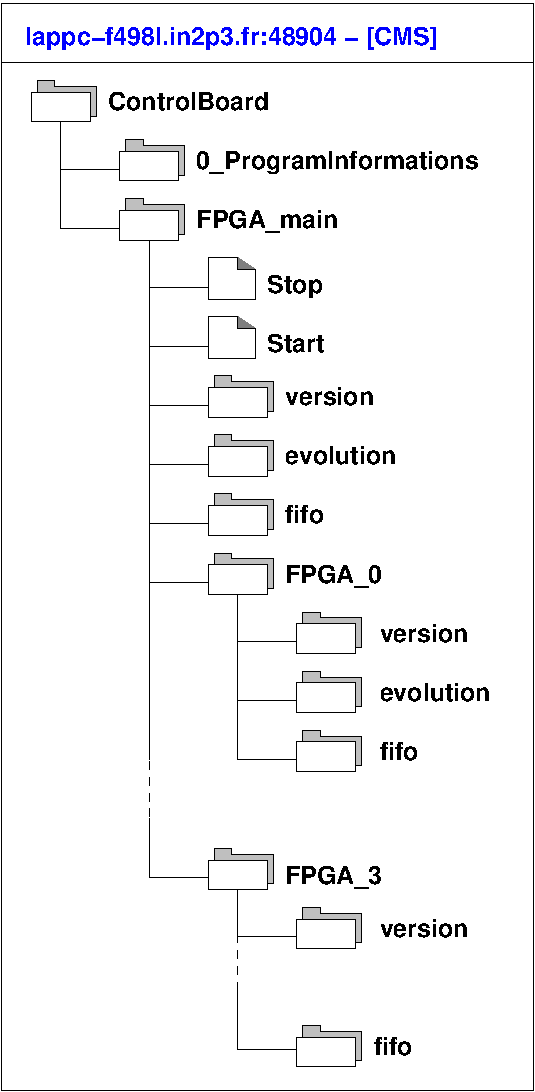
\includegraphics[width=5cm]{appendix/images/MOS_device_example_1.pdf}
\end{center}
\caption{Example of a  device managed through a MOS  server.  The root
  device is named \texttt{ControlBoard}.  First level daughter devices
  are  \texttt{0\_ProgramInformations} and  \texttt{FPGA\_main}.  Here
  the          MOS/OPCUA          server          is          labelled
  \texttt{CMS}.}\label{fig:an:mos_dev_1}
\end{figure}

% TODO


\subsection{Integration of a new device in the Vire environment}

The Vire  API also implements a  mechanism to describe a  hierarchy of
devices.  This  mechanism is independant  of the  one used in  the MOS
system but can  be easily made compatible with it.   This means that a
MOS  hierarchy  of devices  can  be  represented  in Vire.   The  Vire
hierarchy of  devices can  be considered as  some kind  of filesystem,
each device  being a folder with  its unique path, as  shown on figure
\ref{fig:an:mos_dev_2}.   The \emph{methods}  associated to  a devices
(or a datapoint) can be considered as plain executable files stored in
the  device's folder  : they  constitute the  set of  \emph{resources}
associated to the device.


\begin{figure}[h]
\begin{center}
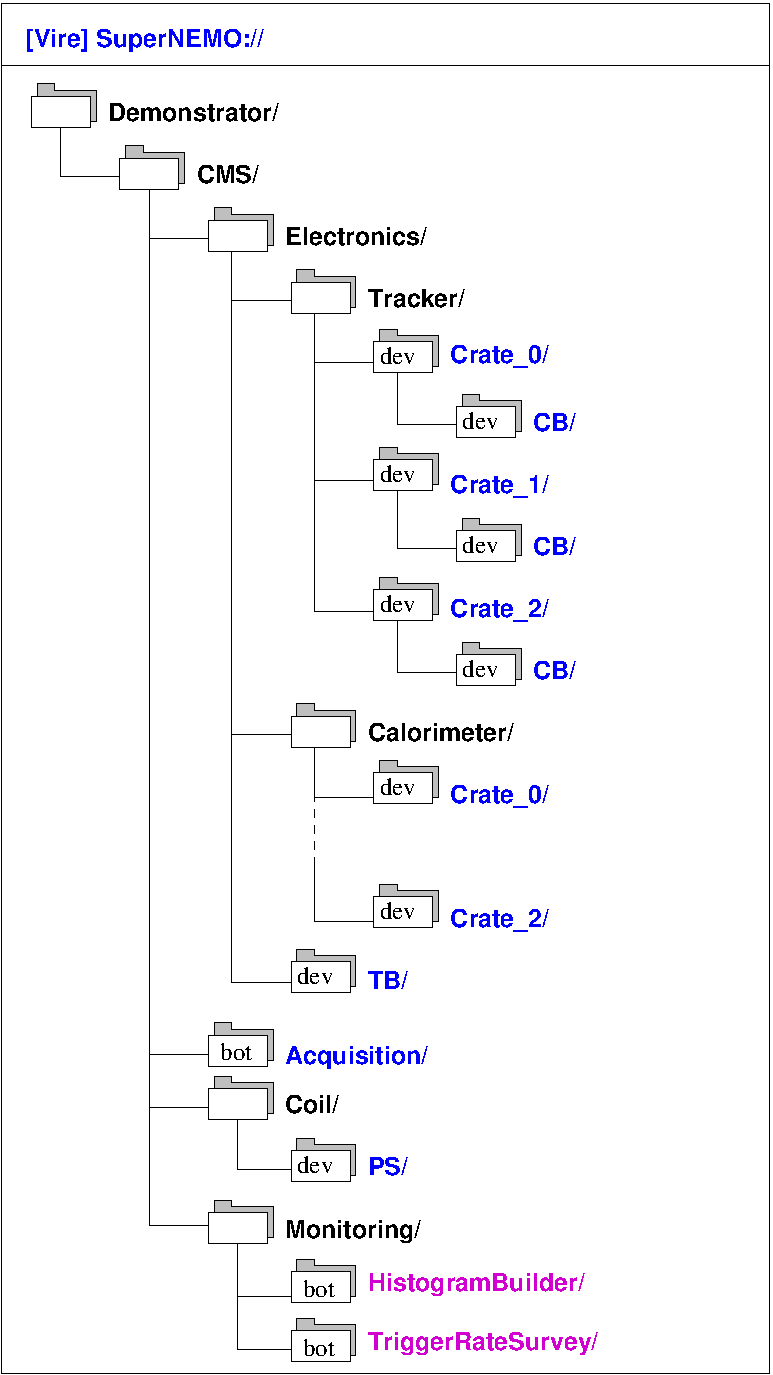
\includegraphics[width=5cm]{appendix/images/MOS_device_example_2.pdf}
\end{center}
\caption{Example of a hierarchy of  devices described by the Vire API.
  The root device is named  \texttt{SuperNEMO:}.  The top level (root)
  device  is  named  \texttt{Demonstrator}.  The  devices  colored  in
  \textcolor{blue}{blue}  are managed  through MOS/OPCUA.  The devices
  colored in \textcolor{magenta}{magenta} are directly embedded in the
  Vire server.  Devices with the \texttt{dev} tag are typical hardware
  device.  Devices  with the  \texttt{bot}  tag  are typical  software
  devices.   The  devices  colored in  \textbf{black}  are  structural
  pseudo-devices used to organize and  present a comprehensive view of
  the hierarchy. }\label{fig:an:mos_dev_2}
\end{figure}

The organisation of this hierarchy of devices is arbitrary and defined
by the designer of the  \emph{Control and Monitoring System}.  What is
important  to  understand  is  that  some  of  these  devices  can  be
associated  to  \emph{hardware  devices}  (a  power  supply  crate,  a
temperature probe\dots) and others  can be \emph{pseudo-devices}, i.e.
pure   software  object   (a   monitoring  robot,   a  file   transfer
daemon\dots).

In the context of the coupling of  the Vire server and the CMS server,
we are  in the event that  some devices are managed  by some MOS/OPCUA
servers and others are managed  in the Vire server itself.  Typically,
\emph{hardware devices}  are systematically managed through  the OPCUA
technology.  Vire has a mechanism to integrate such devices in its own
hierarchy.  This mechanism can  be considered like the \emph{mounting}
of   a   remote   filesystem   from  a   local   filesystem.    Figure
\ref{fig:an:mos_dev_0} illustrates  the case of many  hardware devices
-- managed by MOS -- that are integrated in the Vire system.  From the
Vire point of  view, the user does not see  the implementation details
for such  devices. He  does not  know the identity  of the  MOS server
hosting the device. He does not even know if the device is hosted by a
MOS server.  Devices are simply visible through the standard hierarchy
published by Vire with its  own device naming scheme, regardless their
true location.



\begin{figure}[h]
\begin{center}
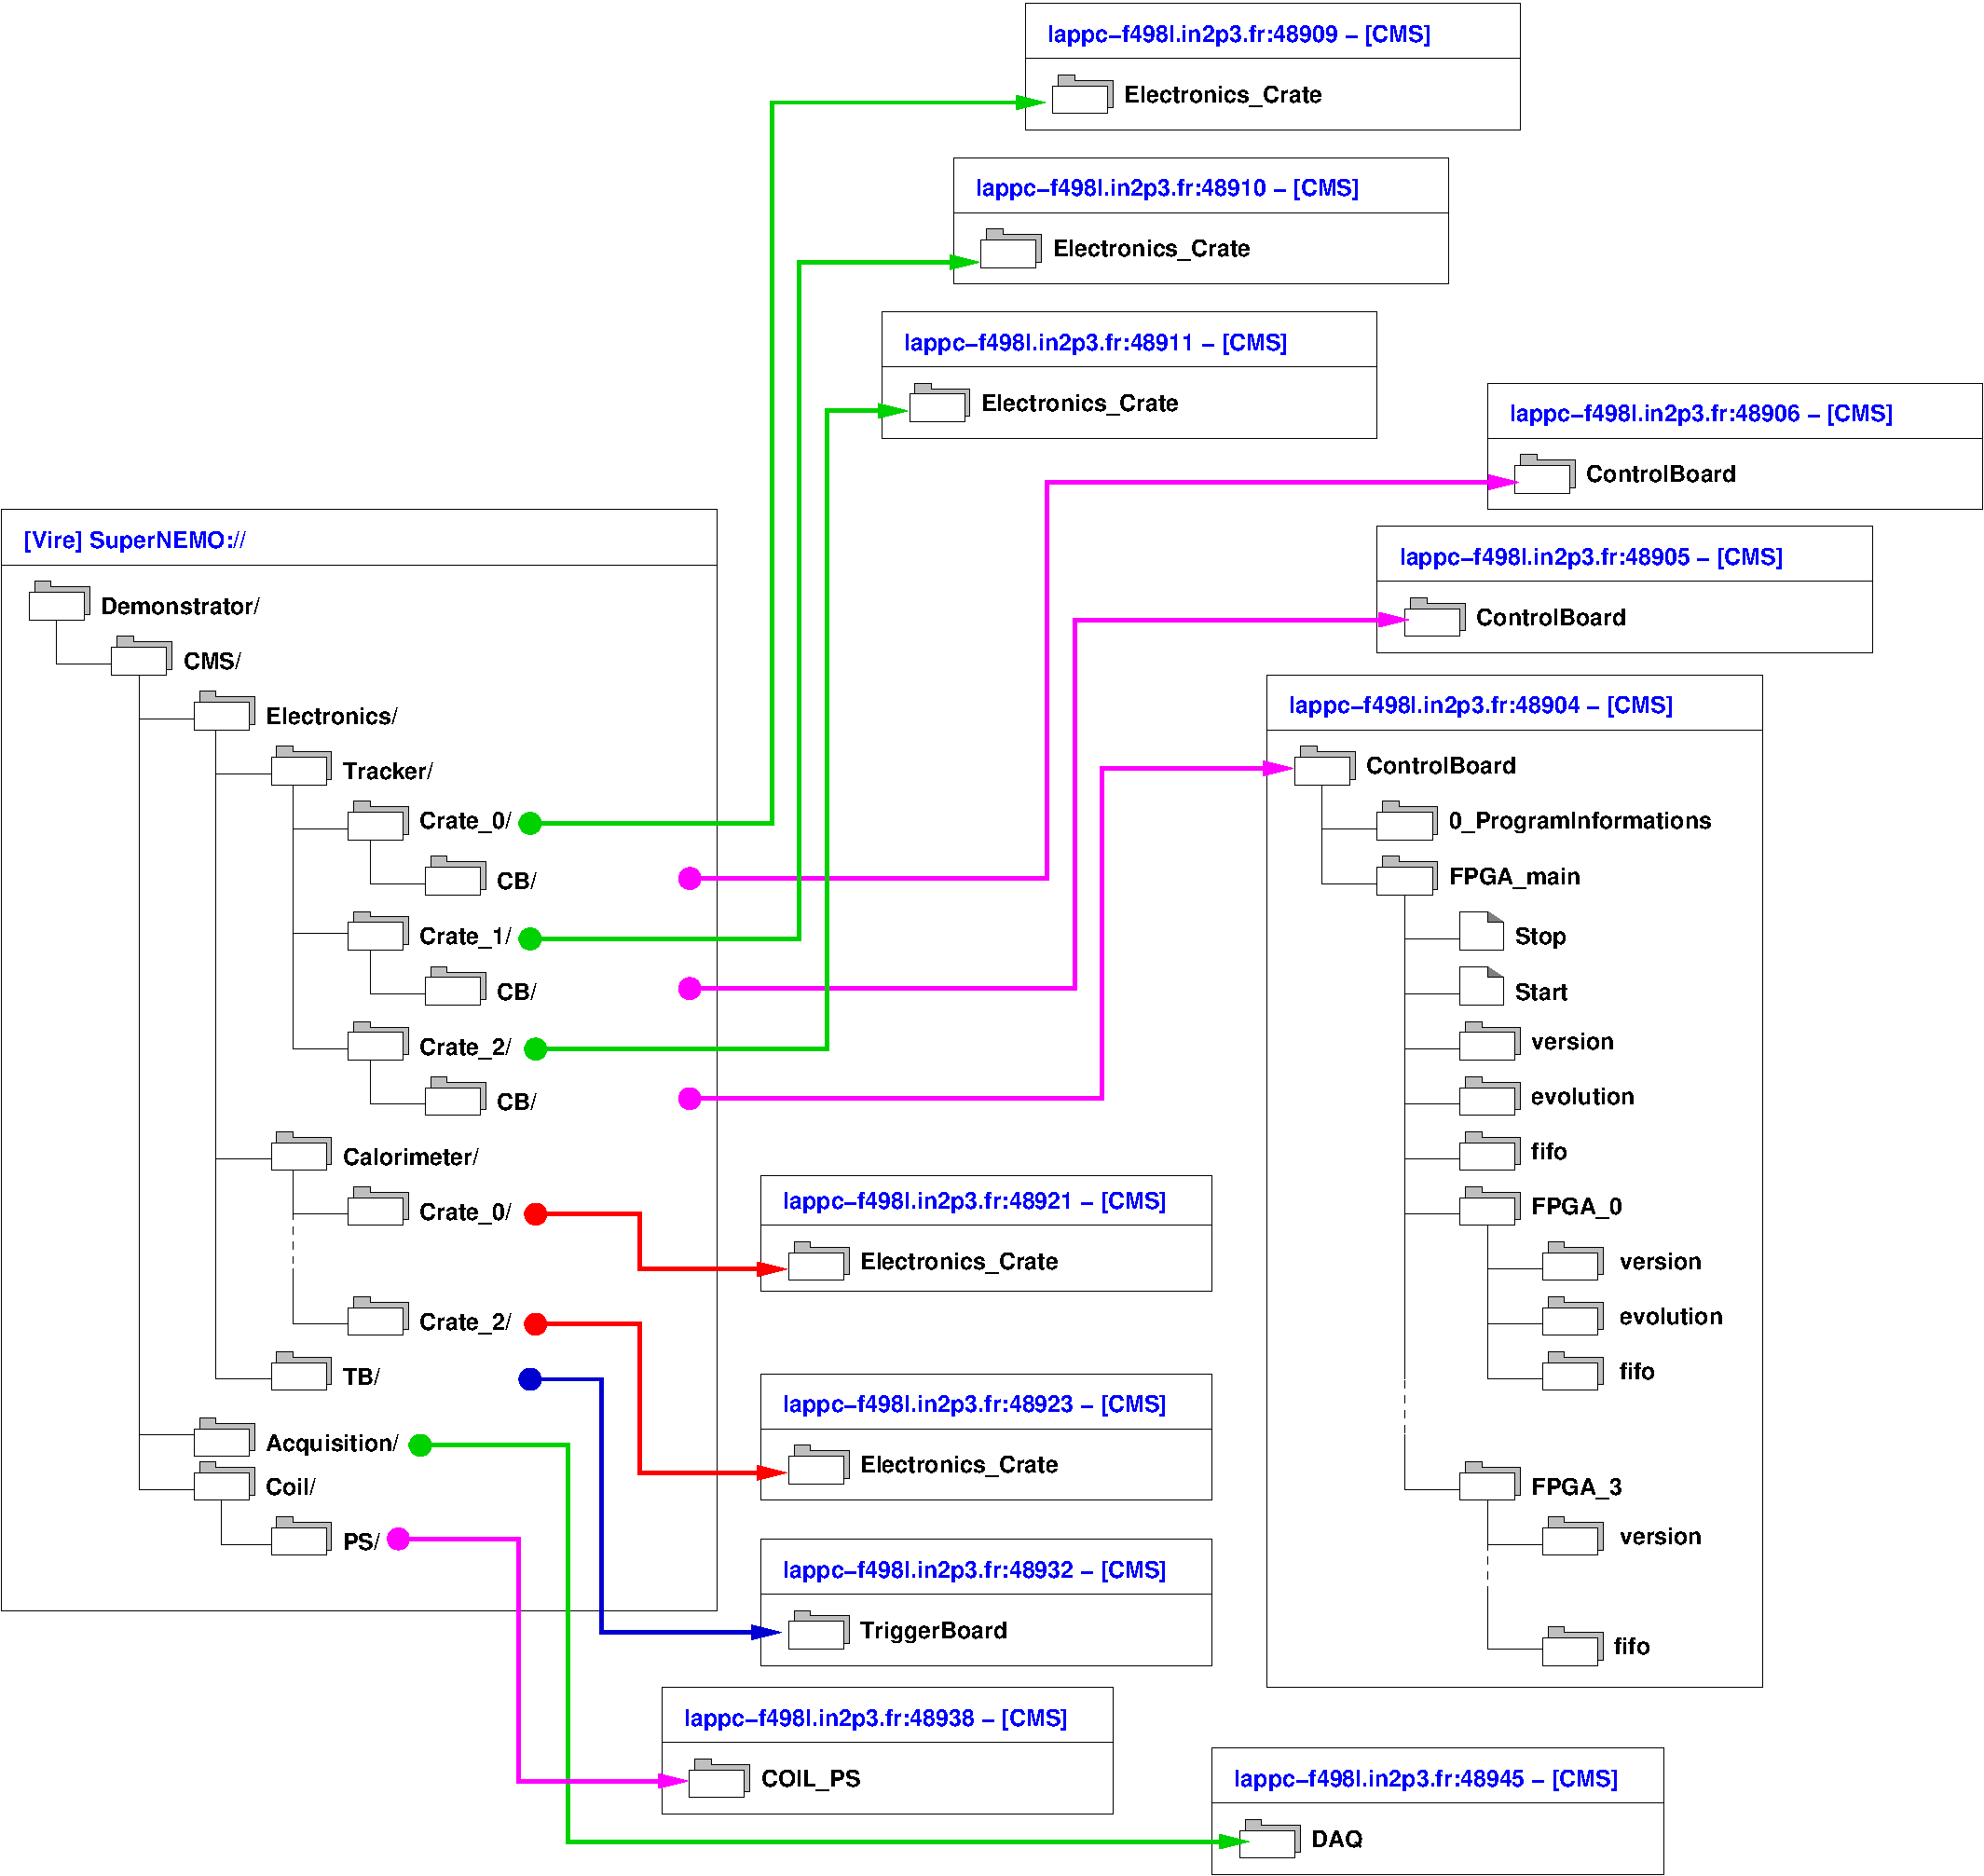
\includegraphics[width=\linewidth]{appendix/images/MOS_device_example_0.pdf}
\end{center}
\caption{The  mounting of  many  MOS device  hierarchies  in the  Vire
  device hierarchy.  Each OPCUA server  runs a simple  hardware device
  that is \emph{mounted} from a specific node with its own path.
%% of  devices described by the Vire API.
%%   The root device is named  \texttt{SuperNEMO:}.  The top level (root)
%%   device is  named \texttt{Demonstrator}. The devices  colored in blue
%%   are managed  through MOS/OPCUA. The  devices colored in  magenta are
%%   directly embedded in the Vire server.  Devices with the \texttt{dev}
%%   tag are typical  hardware device. Devices with  the \texttt{bot} tag
%%   are typical software devices.
}\label{fig:an:mos_dev_0}
\end{figure}




\subsection{Example}

Using  the examples  displayed  in  figure \ref{fig:an:mos_dev_0},  we
consider  in detail  the way  one specific  device managed  by MOS  is
mounted   in  the   Vire   hierarchy.  Figure   \ref{fig:an:mos_dev_3}
illustrates the mounting of a MOS device in Vire.

Here the Vire  server publishes the path of a  device representing the
control board  of the third  electronic crate  for the tracker  of the
SuperNEMO demonstrator module.  The full Vire path of this device is:

\textcolor{blue}{\texttt{SuperNEMO://Demonstrator/CMS/Electronics/Tracker/Crate\_2/CB}}

This is  the only Vire identifier  recognized by user to  address this
device.

On    the   figure,    one    can   see    that    the   MOS    server
\texttt{lappc−f498l.in2p3.fr} (port 48904) hosts a simple device which
is locally named \texttt{ControlBoard}.

When  mounting   this  device  in   the  Vire  hierarchy,   the  local
\texttt{[CMS]}  namespace and  \texttt{ControlBoard} device  names are
hidden and replaced by the Vire device path.  All daughter devices and
datapoints of  the \texttt{CMS/ControlBoard} device are  integrated as
daughters        of        the         Vire        device        named\\
\texttt{SuperNEMO://Demonstrator/CMS/Electronics/Tracker/Crate\_2/CB}.


For example, the \texttt{FPGA\_main} daughter device is now associated
to the following Vire path:

\textcolor{blue}{\texttt{SuperNEMO://Demonstrator/CMS/Electronics/Tracker/Crate\_2/CB/FPGA\_main/}}

and  its  \texttt{Stop} method  is  automatically  addressed with  the
following \emph{leaf} path:

\textcolor{blue}{\texttt{SuperNEMO://Demonstrator/CMS/Electronics/Tracker/Crate\_2/CB/FPGA\_main/Stop}}


\begin{figure}[h]
\begin{center}
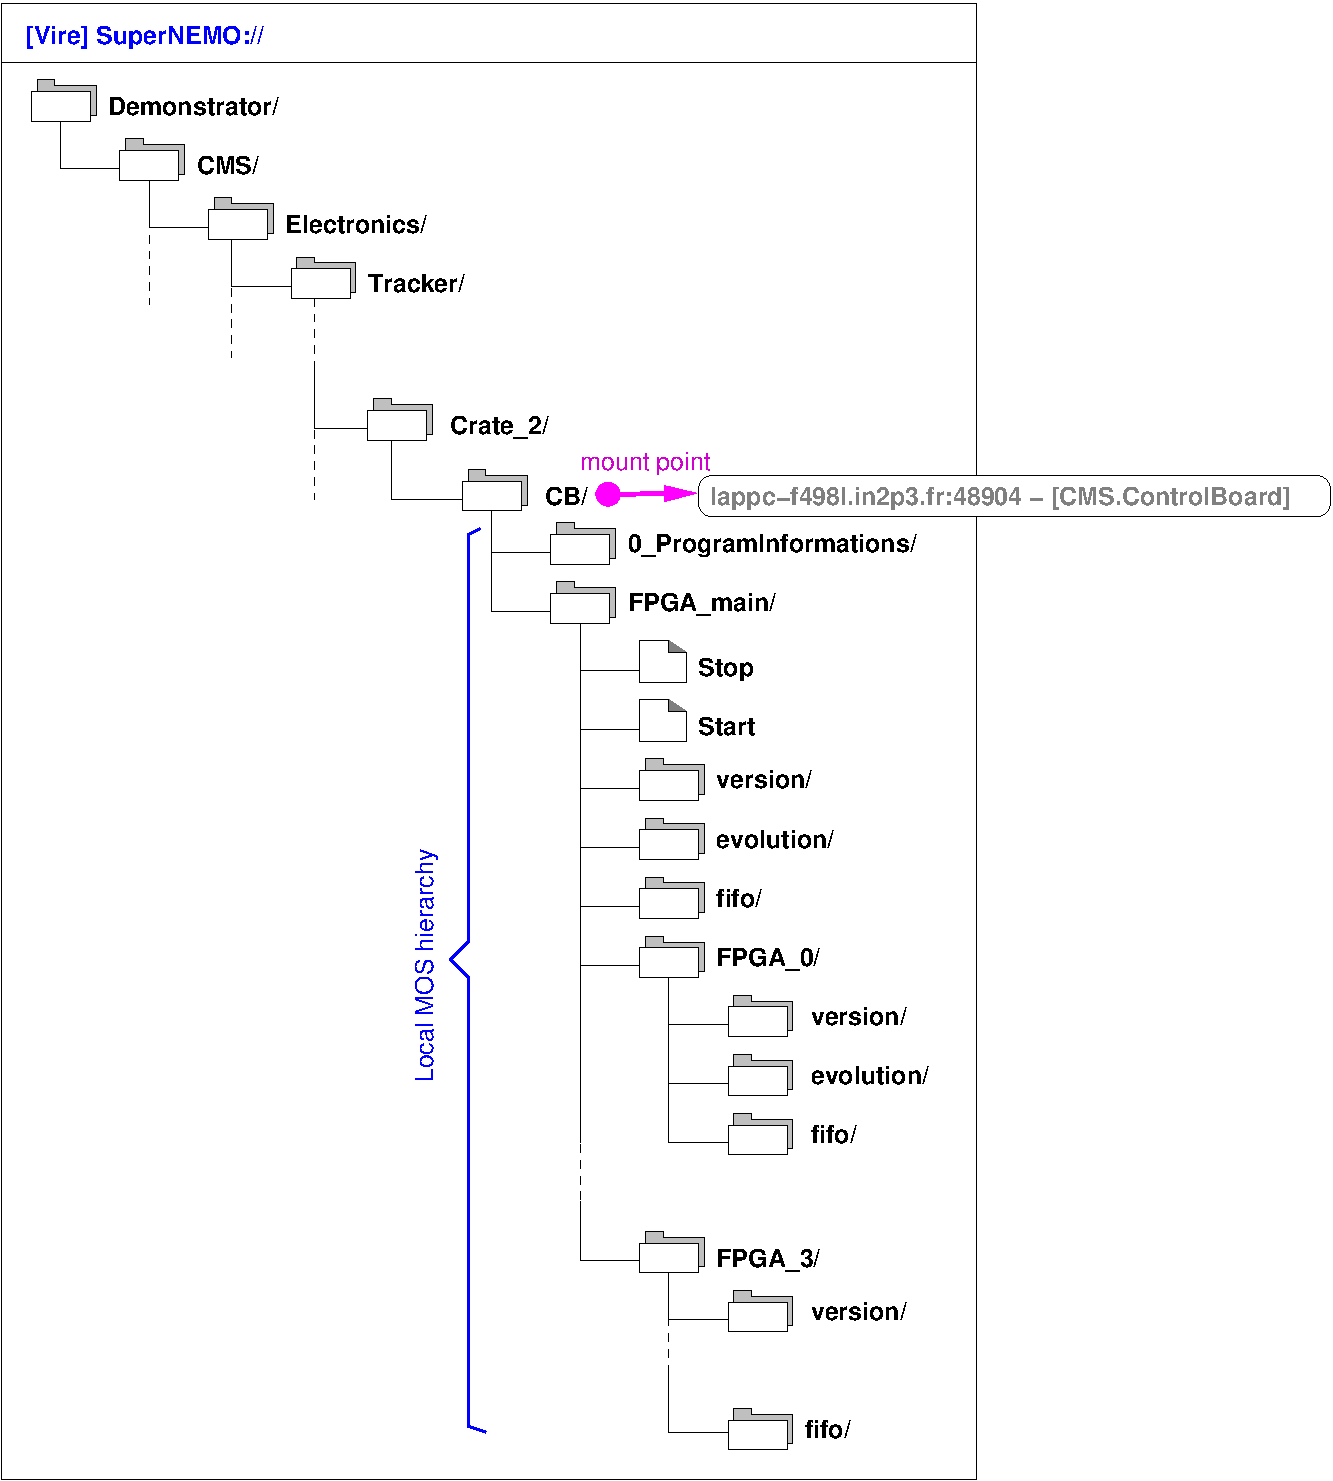
\includegraphics[width=0.8\linewidth]{appendix/images/MOS_device_example_3.pdf}
\end{center}
\caption{The  mounting of  one  MOS device and its local hierarchy  in the  Vire
  device hierarchy.}\label{fig:an:mos_dev_3}
\end{figure}



\subsection{Vire/MOS mapping}

As it can be  seen in the above example, the integration  of a new MOS
device in the Vire system is  achieved through soem kind of filesystem
mounting operation.   Particularly, it is  shown that the MOS  name of
the   mounted  root   device  is   replaced  by   an  arbitrary   Vire
path. However, all daughter  nodes (devices, datapoints) attached from
this root  node have their  relative MOS  names preserved in  the Vire
naming scheme.

Any  resource  (method)  associated  to any  of  such  daughter  nodes
inherits this relative naming scheme.

As Vire applications  describe resources through their  Vire paths, it
is thus needed to build an explicit map that associates resource paths
to MOS address  and name. The CMS  server will be able  to resolve the
MOS server/port and  embedded device associated to  the resource path.

The goal of the \texttt{devices\_launch.conf} file is not only to tell
the CMS server what MOS server should  be loaded and ran at start, but
also  to describe  the  \emph{mounting point/names}  used  by Vire  to
access the resources associated to MOS devices.  From the informations
stored in the  file, an explicit associative array must  be built when
the Vire server connect to the CMS server.  It will play the role of a
resource path resolver  when requests about resources will  be sent by
Vire applications.  This associative array  must be locked  during the
Vire/CMS connection.



%\subsubsection{Preparation of XML device models}

%% \noindent\underline{Pre-condition:}
%% The device is working and validated through the MOS/OPCUA server

%% \begin{enumerate}

%% \item Produce XML décrivant le modèle du device enrichi
%%   des metadata
%% Rédaction du fichier XML décrivant le modèle du device

%% \item Génération des fichiers model du type de device pour Vire

%% \item Génération des fichiers instances resolv.conf

%% \end{enumerate}


\vfill
\pagebreak
\clearpage

% end


\section{Vire messages}\label{app:vire_messages}

Within Vire  and between Vire  components and external  components, we
use  a communication  system  based on  Vire  messages.  This  section
describes the structure of such messages.

\subsection{General structure of a message}

Each message consists in two parts (figure \ref{fig-vire-message-message-cpp}):
\begin{itemize}

\item  the  \emph{header}  is   dedicated  to  generic  and  typicalle
  mandatory  informations  which  document   the  message  itself  and
  arbitrary high-level metadata.

\item  the \emph{body}  of the  message  contains the  real data: the payload.
  The structure of the message body depends on some convention. Vire uses
  its own convention to embed the payload data.

\end{itemize}

\begin{figure}[h]
\vskip 10pt
\small
\begin{Verbatim}[frame=single,xleftmargin=0.cm,label=\fbox{C++}]
struct vire::message::message {
  message_header header; // Header of the message
  message_body   body;   // Body of the message
};
\end{Verbatim}
\normalsize
\caption{The structure of a Vire message object (C++  class:
  \texttt{"vire::message::message"})}\label{fig-vire-message-message-cpp}
\end{figure}

\subsection{The message header}

The header contains (figure \ref{fig-vire-message-message_header-cpp}):
\begin{itemize}

  \item The mandatory \texttt{message\_id}  attribute is an identifier
    of the  message which  document the emitter  and a  unique message
    number.   Each emitter  is  responsible of  the  numbering of  the
    messages it  emits, typically using an  incremental technique. The
    message  number is  a positive  integer, starting  from 0  (figure
    \ref{fig-vire-message-message_identifier-cpp}).

  \item  The \texttt{timestamp}  attribute  encodes the  approximative
    time point when the message was  created. It contains the date and
    the time, using at least microsecond resolution.

    Typically,  with  JSON  encoding  system, it  is  expected  to  be
    formatted as a character string, using the following ISO format:

    \begin{center}
      \texttt{yyyymmddThhmmss.uuuuuu}
    \end{center}

    \noindent where:

    \vskip -10pt
    \begin{itemize}
    \item[\texttt{yyyymmdd} :] encodes year/month/day,
    \item[\texttt{hhmmssd} :] encodes hour/minute/second,
    \item[\texttt{uuuuuu} :] encodes microseconds.
    \end{itemize}

  \item   In   the   case    of   a   \emph{response}   message,   the
    \texttt{in\_reply\_to} attribute is set to identify the associated
    request message.

  \item  The \texttt{asynchronous}  boolean  attribute is  set if  the
    message processing  is explicitely requested  by the source  to be
    asynchronous (non-blocking).  In  RPC transactions, where requests
    are transmitted from one point to  the other, its default value is
    \emph{false}.   It  is possible  to  force  a RPC  transaction  in
    asynchronous mode.   This use  case is documented  elsewhere.  For
    event messaging, this flag is conventionally set to \emph{true}.

  \item  The  \texttt{body\_layout\_id}  attribute  is  the  mandatory
    identifier   of   the   layout   of  the   message   body   (class
    \texttt{"vire::utility::model\_identifier"}).  The  default layout
    for     message     body     inside    the     Vire     API     is
    \texttt{"vire::message::body\_format::typed\_payload"}, with version
    \texttt{"1.0"}                                             (figure
    \ref{fig-vire-utility-model_identifier-cpp}).

\end{itemize}


\begin{figure}[h]
\vskip 10pt
\small
\begin{Verbatim}[frame=single,xleftmargin=0.cm,label=\fbox{C++}]
struct vire::message::message_header {
  message_identifier message_id;     // Message identifier from the emitter.
  std::string        timestamp;      // Timestamp.
  message_identifier in_reply_to;    // Message identifier of the associated
                                     // request message (optional).
  bool               asynchronous,   // Asynchronous flag.
  vire::utility::model_identifier     body_layout_id; // Body layout identifier.
  std::map<std::string, std::string>  metadata;       // Key/value metadata dictionary.
};
\end{Verbatim}
\normalsize
\caption{The  structure  of  a   message  header  object  (C++  class:
  \texttt{"vire::message::message\_header"}).}\label{fig-vire-message-message_header-cpp}
\end{figure}

\begin{figure}[h]
\vskip 10pt
\small
\begin{Verbatim}[frame=single,xleftmargin=0.cm,label=\fbox{C++}]
struct vire::message::message_identifier {
  std::string emitter; // Name identifying the emitter of the message.
  int32_t     number;  // Number identifying the message in the emitter's
                       // message numbering scheme.
};
\end{Verbatim}
\normalsize
\caption{The      structure      of     a      message      identifier
  (C++  class:  \texttt{"vire::message::message\_identifier"}).}
\label{fig-vire-message-message_identifier-cpp}
\end{figure}

\begin{figure}[h]
\vskip 10pt
\small
\begin{Verbatim}[frame=single,xleftmargin=0.cm,label=\fbox{C++}]
struct vire::utility::model_identifier {
  std::string name;    // Name identifying the format of the message.
  std::string version; // String identifying the version of the format.
};
\end{Verbatim}
\normalsize
\caption{The structure of a model identifier (C++  class:  \texttt{"vire::utility::model\_identifier"}.}\label{fig-vire-utility-model_identifier-cpp}
\end{figure}




\begin{figure}[h]
\vskip 10pt
\small
\begin{Verbatim}[frame=single,xleftmargin=0.cm,label=\fbox{JSON}]
{
   "header" : {
      "message_id" : {
         "emitter" : "vire.server",
         "number" : 42
      },
      "timestamp" : "20160930T141408.413443",
      "in_reply_to" : {
         "initialized" : true,
         "value" : {
            "emitter" : "vire.client.0",
            "number" : 23
         }
      },
      "asynchronous" : false,
      "body_layout_id" : {
         "name" : "vire::message::body_format::typed_payload",
         "version" : {
            "initialized" : true,
            "value" : "1.0"
         }
      },
      "metadata" : [
         {
            "key" : "key1",
            "value" : "foo"
         },
         {
            "key" : "key2",
            "value" : "42"
         },
         {
            "key" : "key3",
            "value" : "3.1415899999999999"
         },
         {
            "key" : "key4",
            "value" : "true"
         }
      ]
   }
  "body" : {
      ...
   }
}
\end{Verbatim}
\normalsize
\caption{Example of  a   message  header  object in JSON format.}
\label{fig-vire-message-message_header-json}
\end{figure}

\vfill
\clearpage
\pagebreak

\subsection{The message body}

The    default    message   body    layout    in    Vire   is    named
\texttt{"vire::message::body\_format::typed\_payload"}        (version
\texttt{"1.0"}).   Each  message used  within  the  Vire framework  is
supposed to use this layout.  The general idea is that the body of the
message embeded the  \emph{payload object} that has  to be transmitted
between  two components  of  the system.   \emph{Payload objects}  are
classified in one of the three following categories:

\begin{enumerate}

\item \emph{Request}:  describes a request submitted  by one component
  to another component (generally during a synchronous RPC transaction).

\item  \emph{Response}: describes  the  response to  a former  request
  (generally during a synchronous RPC transaction).

\item \emph{Event}: describes an  arbitrary information record (alarm,
  exception, signal\dots) which is transmitted asynchronously.

\end{enumerate}

Vire implements the following class hierarchy:

\begin{center}
\begin{tikzpicture}
  \node (payload)  at (0,2)  [draw] {\texttt{vire::utility::base\_payload}};
  \node (request)  at (-4,0) [draw] {\texttt{vire::utility::base\_request}};
  \node (response) at (2,0)  [draw] {\texttt{vire::utility::base\_response}};
  \node (event)    at (8,0)  [draw] {\texttt{vire::utility::base\_event}};

  %\draw[style=help lines] (-3,-1) grid (10,4);
  \draw (node cs:name=response,anchor=north) |- (0,1);
  \draw (node cs:name=event,anchor=north)    |- (0,1);
  \draw[->] (node cs:name=request,anchor=north)
  |- (0,1) -| (node cs:name=payload,anchor=south);
\end{tikzpicture}
\end{center}

The requirements for the transmitted object are the following:

\begin{itemize}

\item The  type of the object  must be conventionally associated  to a
  unique     \emph{model      identifier}     object      (see     the
  \texttt{"vire::utility::model\_identifier"} class)  which contains a
  unique   name   (\textit{string    identifier})   and   possibly   a
  \textit{version identifier}.  Each software  component that may send
  or  receive the  object  should agree  on  this type  identification
  scheme.   This   enable  the  use  of   object  factories,  whatever
  programming  langage  is used  on  both  side of  the  communication
  system.

\item  For each  software component,  the object  type must  have some
  dedicated  encoding/decoding  functions  available  (again  whatever
  programming language is used). For example the Vire API supports the
  following encoding formats:

  \begin{itemize}

  \item JSON (MIME  encoding type: \texttt{"application/x-json"}), which
    is supportable by many languages,

  \item  Protobuf  (Google  Protocol   Buffers,  MIME  encoding  type:
    \texttt{"application/x-protobuf"}), which is also widely supported,

  \item   Boost/serialisation   (XML,    text   or   binary   archives
    \texttt{"application/x-boost-serialization-xml"},
    \texttt{"application/x-boost-serialization-text"},
    \texttt{"application/x-boost-serialization-binary"}),    which    in
    principle is supported by C++ only.

  \end{itemize}

  The Protobuf  encoding format will be  used to serialize/deserialize
  the  Vire  messages transported  between  the  Vire server  and  the
  CMS/LAPP server.

\end{itemize}

Vire uses a dedicated layout to represent the body of any message with
its embedded payload object. With this technique, the structure of the
body          contains         two          attributes         (figure
\ref{fig-app-vire-message-message_body-cpp}):

\begin{enumerate}

\item The \texttt{payload\_type\_id} specifies the type of the payload
  object   (figure   \ref{fig-app-vire-utility-model_identifier-cpp}).
  This unique name  is conventionaly fixed for a  given application. A
  version tag allows to support possible evolution of the object type.

\item The  \texttt{payload} is a  handle to  a payload object  of type
  request, response or event.

  %% \begin{itemize}
  %% \item Within  the producer  component of  the message,  the encoding
  %%   function associated to the object  type is responsible to generate
  %%   the JSON stream for the object and store it in the buffer.

  %% \item Within  the consumer  component of  the message,  the decoding
  %%   function associated to the object type is responsible to parse the
  %%   JSON stream stored in the buffer and restore the object in memory.

  %% \end{itemize}

  It is expected  that, on both sides of the  connection, the software
  components can  access dedicated  software plugins which  ensure the
  support  of  various   \emph{payload  object  types}  conventionnaly
  associated  with  their  \emph{payload type  identifiers}  and  also
  providing JSON and/or Protobuf encoding/decoding functionalities.

  %% The   system  allows  to  support
  %% modification  in the  structure of  the objects  thanks to  version
  %% tagging.

\end{enumerate}

\begin{figure}[h]
\vskip 10pt
\small
\begin{Verbatim}[frame=single,xleftmargin=0.cm,label=\fbox{C++}]
struct message_body {
  vire::utility::model_identifier     payload_type_id; // Object type identifier.
  const vire::utility::base_payload * payload;         // Handle to a payload object.
};
\end{Verbatim}
\normalsize
\caption{The structure of a message body object (C++).}
\label{fig-app-vire-message-message_body-cpp}
\end{figure}

\begin{figure}[h]
\vskip 10pt
\small
\begin{Verbatim}[frame=single,xleftmargin=0.cm,label=\fbox{JSON}]
{
  "header" : {
    ...
  },
  "body" : {
    "payload_type_id" : {
      "name" : "vire::message::testing::error_event",
      "version" : {
        "initialized" : false
      }
    },
    "payload" : {
      "timestamp" : "20160930T141743.759085"
      "err" : {
        "code" : 3,
        "message" : "A basic error"
      },
    }
  }
}
\end{Verbatim}
\normalsize
\caption{Example of  a   message  body  object in JSON format.}
\label{fig-vire-message-message_body-json}
\end{figure}

\vfill
\clearpage
\pagebreak

% end

%\input{appendix/app_json_fmt.tex}

\section{The \emph{Protocol Buffers} format}\label{app:protobuf_fmt}

\subsection{Introduction}

The  Google  Protocol Buffers  (\emph{protobuf})  library  is used  to
represent the objects that are exchanged between the Vire clients, the
Vire server and the CMS server.  The  version 3 of the format is used,
implying   at   least   version   3.0.0  (September   2016)   of   the
\emph{protobuf} library.

Each  data   structure  of  interest   can  be  described   through  a
\texttt{.proto}  file  from  which  stub files  can  be  automatically
generated  with the  \texttt{protoc} compiler.  For Vire  and its  CMS
interface, the C++ and Java programming languages will be used.


A  collection of  \texttt{.proto}  files are  provided  with the  Vire
library to represent all kind  of data structures transferable between
networked agents  (Vire server,  Vire clients, CMS/LAPP  server).  The
objects of  the highest level  are named \emph{payload  objects} (like
\emph{request},  \emph{response} and  \emph{event} objects).   They
are composed of attributes of more basic data structures.

\subsection{Example}

The following  class diagram  illustrates two data  structures defined
within the Vire library with an inheritance relationship between them.

\begin{center}
  \begin{tikzpicture}
    \node (base)     at (0,1.5)  [draw] {\texttt{vire::utility::base\_error}};
    \node (setup)    at (0,0)  [draw] {\texttt{vire::utility::invalid\_setup\_id\_error}};

    \draw[->]   (node cs:name=setup,anchor=north) |- (0,1);
    |- (0,1) -| (node cs:name=base,anchor=south);
  \end{tikzpicture}
\end{center}

The \texttt{vire::utility::base\_error}  is the  parent class  for all
\emph{error}  objects.   It  contains   two  attributes:   an  integer
\emph{error code}  and a  character string describing  the \emph{error
  message}.

The   \texttt{vire::utility::invalid\_setup\_id\_error}  class   is  a
specialized error class  which represents explicitely an  error due to
an identification  failure of  the experimental setup.   It implements
additional mutually exclusive attributes: the \emph{unrecognized name}
of the setup or the \emph{unrecognized version} of the setup.

This   example  illustrates   the  protobuf   representation  of   the
\texttt{vire::utility::base\_error}  in the  Vire  library, using  the
\texttt{"vire/utility/BaseError.proto"} file:

\small
\begin{Verbatim}[frame=single,xleftmargin=0.cm,label=\fbox{protobuf}]
  syntax = "proto3";
  package vire.utility; // Namespace

  message BaseError {

    // reserved 1; // Reserved for _base message

    // Attributes:
    int32  code           = 100; // The error code
    string message_format = 101; // The error description message

  }
\end{Verbatim}
\normalsize

\vfill
\clearpage
\pagebreak

\subsection{Vire protobuf conventions}

Vire uses the following conventions:

\begin{enumerate}

\item
  The member index  \texttt{1} is reserved to represent the  link of a
  class to its main base/parent class (if any).  It is not used if the
  data structure does not inherit any data structure.
  If a data structure naturally inherits another one, it is thus possible
  to  represent the  inheritance  relationship as  illustrated with  the
  \texttt{"vire/utility/InvalidSetupIdError.proto"}      file      which
  represents the \texttt{vire::utility::invalid\_setup\_id\_error} class
  in the Vire library:

  \small
  \begin{Verbatim}[frame=single,xleftmargin=0.cm,label=\fbox{protobuf}]
    syntax = "proto3";
    package vire.utility; // Namespace

    import "vire/utility/BaseError.proto"; // Dependency

    message InvalidSetupIdError {

      BaseError _base = 1; // The base class

      // Additional attributes:
      oneof detail { // Mutual exclusion
        string invalid_setup_name    = 100; // The failed setup name
        string invalid_setup_version = 101; // The failed setup version
      }

    }
  \end{Verbatim}
  \normalsize

\item The  \texttt{\_base} member  is conventionally  used to  represent the
  inheritance   relationship    from   a   data   structure    of   type
  \texttt{"vire.utility.BaseError"}.

\item Member indexes from \texttt{2}  to \texttt{99} are also reserved
  for possible future usage (multiple inheritance, metadata\dots).

\item
  The first member of the data structure must start at index \texttt{100}.

\end{enumerate}

\vfill
\clearpage
\pagebreak

% end


\section{Vire payload objects}\label{app:payload}

\subsection{Introduction}

As  mentioned in  appendix \ref{app:protobuf_fmt},  Vire messages  are
wrappers for \emph{payload objects}.  Each  type of payload object can
be represented  through the \emph{protobuf} mechanism.   The following
class hierarchy shows the base architecture used to define new payload
objects.

\begin{center}
\begin{tikzpicture}
  \node (payload)  at (0,2)   [draw] {\texttt{vire::utility::base\_payload}};
  \node (request)  at (-4,0)  [draw] {\texttt{vire::utility::base\_request}};
  \node (response) at (2,0)   [draw] {\texttt{vire::utility::base\_response}};
  \node (event)    at (8,0)   [draw] {\texttt{vire::utility::base\_event}};
  \node (my)       at (-4,-2) [draw] {\texttt{my\_request}};
  \node (your)     at (2,-2)  [draw] {\texttt{your\_response}};
  \node (its)    at (8,-2)    [draw] {\texttt{its\_alarm}};

  %\draw[style=help lines] (-6,-2) grid (10,2);
  \draw (node cs:name=response,anchor=north) |- (0,1);
  \draw (node cs:name=event,anchor=north)    |- (0,1);
  \draw[->] (node cs:name=request,anchor=north)
  |- (0,1) -| (node cs:name=payload,anchor=south);
  \draw[->] (node cs:name=my,anchor=north)
  |- (-4,-1) -| (node cs:name=request,anchor=south);
  \draw[->] (node cs:name=your,anchor=north)
  |- (2,-1) -| (node cs:name=response,anchor=south);
  \draw[->] (node cs:name=its,anchor=north)
  |- (8,-1) -| (node cs:name=event,anchor=south);
\end{tikzpicture}
\end{center}


\begin{center}
\vskip 10pt
\small
\begin{tabular}{|l|l|l|}
  \hline
  \textbf{Vire C++ class} & \textbf{protobuf message type} & \textbf{protobuf definition file} \\
  \hline
  \hline
  \multicolumn{3}{|c|}{\emph{general types}} \\
  \hline
  boost::posix\_time::ptime & google.protobuf.Timestamp & google/protobuf/timestamp.proto \\
  \hline
  \hline
  \multicolumn{3}{|c|}{\emph{identifier types}} \\
  \hline
  vire::utility::base\_identifier & vire.utility.Baseidentifier & vire/utility/Baseidentifier.proto \\
  \hline
  vire::utility::instance\_identifier & vire.utility.InstanceIdentifier & vire/utility/InstanceIdentifier.proto \\
  \hline
  vire::utility::model\_identifier & vire.utility.ModelIdentifier & vire/utility/ModelIdentifier.proto \\
  \hline
  \hline
  \multicolumn{3}{|c|}{\emph{error types}} \\
  \hline
  vire::utility::base\_error & vire.utility.BaseError & vire/utility/BaseError.proto \\
  \hline
  vire::utility::invalid\_context\_error & vire.utility.InvalidContextError & vire/utility/InvalidContextError.proto \\
  \hline
  vire::utility::invalid\_setup\_id\_error & vire.utility.InvalidSetupIdError & vire/utility/InvalidSetupIdError.proto \\
  \hline
  \hline
  \multicolumn{3}{|c|}{\emph{payload types}} \\
  \hline
  vire::utility::base\_payload & vire.utility.BasePayload & vire/utility/BasePayload.proto \\
  \hline
  vire::utility::base\_request & vire.utility.BaseRequest & vire/utility/BaseRequest.proto \\
  \hline
  vire::utility::base\_response & vire.utility.BaseResponse & vire/utility/BaseResponse.proto \\
  \hline
  vire::utility::base\_event & vire.utility.BaseEvent & vire/utility/BaseEvent.proto \\
  \hline
  vire::utility::base\_alarm & vire.utility.BaseAlarm & vire/utility/BaseAlarm.proto \\
  \hline
  \hline
  \multicolumn{3}{|c|}{\emph{messenging types}} \\
  \hline
  vire::message::message\_identifier & vire.message.MessageIdentifier & vire/message/MessageIdentifier.proto \\
  \hline
  vire::message::msg\_header & vire.message.MsgHeader & vire/message/MsgHeader.proto \\
  \hline
  vire::message::msg\_body & vire.message.MsgBody & vire/message/MsgBody.proto \\
  \hline
  vire::message::message & vire.message.Message & vire/message/Message.proto \\
  \hline
\end{tabular}
\normalsize
\end{center}


\begin{center}
\vskip 10pt
\small
\begin{tabular}{|l|l|l|}
  \hline
  \multicolumn{3}{|c|}{\emph{Resource management related types}} \\
  \hline
  vire::cms::resource\_status\_record & vire.cms.ResourceStatusRecord & vire/cms/ResourceStatusRecord.proto \\
  \hline
  vire::cms::resource\_fetch\_status\_request & vire.cms.ResourceFetchStatusRequest & vire/cms/ResourceFetchStatusRequest.proto \\
  \hline
  vire::cms::resource\_fetch\_status\_success\_response & vire.cms.ResourceFetchStatusSuccessResponse & vire/cms/ResourceFetchStatusSuccessResponse.proto \\
  \hline
  vire::cms::resource\_fetch\_status\_failure\_response & vire.cms.ResourceFetchStatusFailureResponse & vire/cms/ResourceFetchStatusFailureResponse.proto \\
  \hline
  vire::cms::resource\_exec\_request & vire.cms.ResourceExecRequest & vire/cms/ResourceExecRequest.proto \\
  \hline
  vire::cms::resource\_exec\_success\_response & vire.cms.ResourceExecSuccessResponse & vire/cms/ResourceExecSuccessResponse.proto \\
  \hline
  vire::cms::resource\_exec\_failure\_response & vire.cms.ResourceExecFailureResponse & vire/cms/ResourceExecFailureResponse.proto \\
  \hline
  vire::cms::resource\_exec\_non\_blocking\_request & vire.cms.ResourceExecNonBlockingRequest & vire/cms/ResourceExecNonBlockingRequest.proto \\
  \hline
  vire::cms::resource\_exec\_non\_blocking\_ack\_response & vire.cms.ResourceExecNonBlockingAckResponse & vire/cms/ResourceExecNonBlockingAckResponse.proto \\
  \hline
  vire::cms::resource\_exec\_non\_blocking\_noack\_response & vire.cms.ResourceExecNonBlockingNoackResponse & vire/cms/ResourceExecNonBlockingNoackResponse.proto \\
  \hline
  vire::cms::resource\_exec\_non\_blocking\_success\_event & vire.cms.ResourceExecNonBlockingSuccessEvent & vire/cms/ResourceExecNonBlockingSuccessEvent.proto \\
  \hline
  vire::cms::resource\_exec\_non\_blocking\_failure\_event & vire.cms.ResourceExecNonBlockingFailureEvent & vire/cms/ResourceExecNonBlockingFailureEvent.proto \\
  \hline
  vire::cms::resource\_exec\_error & vire.cms.ResourceExecError & vire/cms/ResourceExecError.proto \\
  \hline
  vire::cms::invalid\_status\_error & vire.cms.ResourceExecError & vire/cms/ResourceExecError.proto \\
  \hline
  %% vire::cms::invalid\_credentials\_error & vire.cms.InvalidCredentialsError & vire/cms/InvalidCredentialsError.proto \\
  %% \hline
  %% vire::cms::invalid\_user\_error & vire.cms.InvalidUserError & vire/cms/InvalidUserError.proto \\
  %% \hline
  vire::cms::invalid\_resource\_error & vire.cms.InvalidUserError & vire/cms/InvalidUserError.proto \\
  \hline
  vire::cms::no\_pubsub\_resource\_error & vire.cms.NoPubsubResourceError & vire/cms/NoPubsubResourceError.proto \\
  \hline
  \hline
  \multicolumn{3}{|c|}{\emph{Resource pub/sub management types}} \\
  \hline
  vire::cms::resource\_pubsub\_subscribe\_request & vire.cms.ResourcePubsubSubscribeRequest & vire/cms/ResourcePubsubSubscribeRequest.proto \\
  \hline
  vire::cms::resource\_pubsub\_subscribe\_success\_response & vire.cms.ResourcePubsubSubscribeRSuccessResponse & vire/cms/ResourcePubsubSubscribeRSuccessResponse.proto \\
  \hline
  vire::cms::resource\_pubsub\_subscribe\_failure\_response & vire.cms.ResourcePubsubSubscribeRFailureResponse & vire/cms/ResourcePubsubSubscribeRSuccessResponse.proto \\
  \hline
  \hline
  \multicolumn{3}{|c|}{\emph{Vire/CMS server interface types}} \\
  \hline
  vire::cmsinterface::connection\_request & vire.cmsinterface.ConnectionRequest & vire/cmsinterface/ConnectionRequest.proto \\
  \hline
  vire::cmsinterface::connection\_success\_response & vire.cmsinterface.ConnectionSuccessResponse & vire/cmsinterface/ConnectionSuccessResponse.proto \\
  \hline
  vire::cmsinterface::connection\_failure\_response & vire.cmsinterface.ConnectionFailureResponse & vire/cmsinterface/ConnectionFailureResponse.proto \\
  \emph{embedded:} unknown\_resources\_error & .UnknownResourcesError &  \\
  \hline
  vire::cmsinterface::disconnection\_request & vire.cmsinterface.DisconnectionRequest & vire/cmsinterface/DisconnectionRequest.proto \\
  \hline
  vire::cmsinterface::disconnection\_success\_response & vire.cmsinterface.DisconnectionSuccessResponse & vire/cmsinterface/DisconnectionSuccessResponse.proto \\
  \hline
  %% \hline
  %% vire::cmsinterface::disconnection\_failure\_response & vire.cmsinterface.DisconnectionFailureResponse & vire/cmsinterface/DisconnectionFailureResponse.proto \\
\end{tabular}
\normalsize
\end{center}

\subsection{Basic data structures}

Any  payload object  (request, response  or event)  generally contains
some information records which are  specific to the functionalities of
the  payload  object they  belong.   These  records are  of  arbitrary
types. Of course they should be  translatable in terms of the protobuf
library.
%Of course they can be (de)serialized using JSON.
Some of these types are very  general and defined within the Vire core
API itself because they are reused by various payload objects not only
through  the Vire-CMS/LAPP  interface  but also  between  Vire clients  and
servers, independently  of the  CMS/LAPP server.  However,  the use  of the
Protocol Buffers interface makes possible  to publish the interface of
such data to the outside world, including the CMS/LAPP server in priority.

%% Other one are specific to the Vire/CMS interface and thus managed only
%% in the \texttt{Vire\_CMSInterface} API.
These  types  are considered  as  \emph{basic}.  Among them  we  find:
generic error  types, generic  identifier types,  timestamps, resource
status records\dots We propose to describe them in this section.

Once a sufficient collection of  basic data record types is available,
it  is possible  to describe  high  level payload  object types  which
aggregate attributes of such types.

Other record  types are specific to  some payload objects and  will be
never  used outside  the scope  of these  payload objects.   Such data
structures will be  explicitely declared with the  payload object they
belong to, likely as embedded types/classes.


\subsubsection{Errors}

Some  \emph{response} or  \emph{event} payload  objects may  contain a
specific  error  record  object.   A  \emph{failure  response}  or  an
\emph{exception  event}  object will  generally  embed  such an  error
record object.

Each  \emph{error record}  is represented  by an  instance of  a given
error type.   Each of  the error  types defined  in Vire  inherits the
\texttt{vire::utility::base\_error}      base       class      (figure
\ref{fig-app-payload-base_error})   which   contains   the   following
attributes:

\begin{itemize}

\item the error code: A non zero  integer which is set to 1 by default
  (indicating  a  generic  failure  case).   The  error  code  can  be
  conventionally  set to  any positive  integer value  to represent  a
  specific error case, depending on the context.

\item the error  message: an optional human  readable character string
  which documents the error as usefully as possible.

\end{itemize}

\begin{figure}[h]
\vskip 10pt
\small
\begin{Verbatim}[frame=single,xleftmargin=0.cm,label=\fbox{C++}]
struct vire::utility::base_error
{
  // Attributes:
  int         code;           // Error code (>0).
  std::string message_format; // Error message (optional).
};
\end{Verbatim}
\normalsize
\caption{The structure of a \texttt{"vire::utility::base\_error"} object
  (C++).}
\label{fig-app-payload-base_error}
\end{figure}


%% An example of JSON formatted basic error object is given in figure
%% \ref{fig-app-payload-base_error-1}.
%%
%% \begin{figure}[h]
%% \vskip 10pt
%% \small
%% \begin{Verbatim}[frame=single,xleftmargin=0.cm,label=\fbox{\texttt{JSON}}]
%% {
%%   "code" : "42",
%%   "message_format" : "Invalid AMQP server port=[2341]"
%% }
%% \end{Verbatim}
%% \normalsize
%% \caption{JSON  formatted  basic  error  object  (class
%%   \texttt{vire::utility::base\_error}.}
%% \label{fig-app-payload-base_error-1}
%% \end{figure}

Several type of generic errors are defined in Vire:


\begin{center}
\begin{tikzpicture}
  \node (base)     at (0,2)  [draw] {\texttt{vire::utility::base\_error}};
  \node (context)  at (-4,0) [draw] {\texttt{vire::utility::invalid\_context\_error}};
  \node (setup)    at (0,-1)  [draw] {\texttt{vire::utility::invalid\_setup\_id\_error}};
  \node (resource) at (4,0)  [draw] {\texttt{vire::cms::invalid\_resource\_error}};
  \node (user)     at (8,-1)  [draw] {\texttt{vire::cms::invalid\_user\_error}};

  \draw     (node cs:name=setup,anchor=north)    |- (0,1);
  \draw     (node cs:name=resource,anchor=north) |- (0,1);
  \draw     (node cs:name=user,anchor=north)     |- (0,1);
  \draw[->] (node cs:name=context,anchor=north)
  |- (0,1) -| (node cs:name=base,anchor=south);
\end{tikzpicture}
\end{center}

\noindent
Here are a few error object types defined in Vire.  Some types belongs
to the \texttt{utility} namespace, other  ones are in the \texttt{cms}
namespace:

\begin{itemize}

\item \texttt{"vire::utility::invalid\_context\_error"} : occurs typically when
  the general context of the execution of a given resource is not adapted.\\
  It is mapped to the \texttt{"vire.utility.InvalidContextError"} protobuf record.

\item \texttt{"vire::utility::invalid\_setup\_id\_error"} : occurs in case
  of an invalid identification of the experimental setup managed
  by the Vire or CMS server.\\
  It is mapped to the \texttt{"vire.utility.InvalidSetupIdError"} protobuf record.

\item \texttt{"vire::cms::invalid\_resource\_error"} : occurs in case
  of an invalid identification of a resource.\\
  It is mapped to the  \texttt{"vire.cms.InvalidResourceError"} protobuf record.

\item \texttt{"vire::cms::invalid\_status\_error"}: occurs when an attempt
  to access a resource that has not the proper status.\\
  It is mapped to the  \texttt{"vire.cms.InvalidStatusError"} protobuf record.

\item \texttt{"vire::cms::invalid\_user\_error"} : occurs in case
  of an invalid identification of an user.\\
  It is mapped to the  \texttt{"vire.cms.InvalidUserError"} protobuf record.

\item \texttt{"vire::cms::invalid\_credentials\_error"} : occurs in case
  of user authentication error.\\
  It is mapped to the  \texttt{"vire.cms.InvalidCredentialsError"} protobuf record.

\item \texttt{"vire::cms::resource\_exec\_error"} : occurs in case
  of error at the execution of a given resource.\\
  It is mapped to the  \texttt{"vire.cms.ResourceExecError"} protobuf record.

\end{itemize}



\subsubsection{Object and type identifiers}

Vire  uses  some dedicated  classes  to  represent the  identifier  of
various objects  (or \emph{instances})  as well  as various  types (or
\emph{models})  of components.  Vire  implements  the following  class
hierarchy:

\begin{center}
\begin{tikzpicture}
  \node (base)  at (0,2)  [draw] {\texttt{vire::utility::base\_identifier}};
  \node (instance)  at (-4,0) [draw] {\texttt{vire::utility::instance\_identifier}};
  \node (model) at (4,0)  [draw] {\texttt{vire::utility::model\_identifier}};

  \draw (node cs:name=model,anchor=north) |- (0,1);
\draw[->] (node cs:name=instance,anchor=north)
  |- (0,1) -| (node cs:name=base,anchor=south);
\end{tikzpicture}
\end{center}

The          \texttt{vire::utility::base\_identifier}          (figure
\ref{fig-app-payload-base_identifier}) class is  a pure abstract class
that cannot be instantiated. However  it contains a mandatory name and
an  optional  version description  which  are  used by  all  inherited
classes:

\begin{itemize}

\item The   \texttt{vire::utility::instance\_identifier}    concrete   class
inherits  \texttt{vire::utility::base\_identifier}  and   is  used  to
identify \underline{unique instances of objects} known by the system.

\item The  \texttt{vire::utility::model\_identifier}   concrete  class  also
inherits  \texttt{vire::utility::base\_identifier}  and   is  used  to
identify \underline{types of objects} registered in the system.

\end{itemize}

The only difference between these two classes is the validation scheme
of  the name  attribute.

\begin{figure}[h]
\vskip 10pt
\small
\begin{Verbatim}[frame=single,xleftmargin=0.cm,label=\fbox{C++}]
struct base_identifier
{
  // Attributes:
  std::string name;    // The mandatory name uniquely identifying the object or
                       // the type of object.
  std::string version; // An optional character string representing the version
                       // of the object type.
};
\end{Verbatim}
\normalsize
\caption{The structure of the \texttt{vire::utility::base\_identifier}
  class (C++).}
\label{fig-app-payload-base_identifier}
\end{figure}

%%  Figure  \ref{fig-app-payload-identifier-json}
%% shows an example of instance indentifier.
%% \begin{figure}[h]
%% \vskip 10pt
%% \small
%% \begin{Verbatim}[frame=single,xleftmargin=0.cm,label=\fbox{\texttt{JSON}}]
%% {
%%   "name" : "vire::resource::invalid_resource_error",
%%   "version" : "1.0"
%% }
%% \end{Verbatim}
%% \normalsize
%% \caption{JSON  formatted class identifier  object (class
%%   \texttt{vire::utility::model\_identifier}).   Here one  identifies a
%%   specific error type.}
%% \label{fig-app-payload-identifier-json}
%% \end{figure}


\vfill
\pagebreak
\clearpage

\subsubsection{Resource related objects}

\begin{itemize}

\item
Class \texttt{vire::cms::invalid\_resource\_error} (figure \ref{fig-app-payload-invalid_resource_error}).

\begin{center}
\begin{tikzpicture}
  \node (base)  at (0,2)  [draw] {\texttt{vire::utility::base\_error}};
  \node (ire)  at (0,0) [draw] {\texttt{vire::cms::invalid\_resource\_error}};
  \draw[->] (node cs:name=ire,anchor=north)
  |- (0,1) -| (node cs:name=base,anchor=south);
\end{tikzpicture}
\end{center}

\begin{figure}[h]
\vskip 10pt
\small
\begin{Verbatim}[frame=single,xleftmargin=0.cm,label=\fbox{C++}]
struct vire::cms::invalid_resource_error : public vire::utility::base_error
{
  // Attributes:
  std::string invalid_resource_path; // Invalid resource path
  std::string invalid_resource_id;   // Invalid resource internal ID (Vire server only)
};
\end{Verbatim}
\normalsize
\caption{The structure  of a invalid resource error object (C++).}
\label{fig-app-payload-invalid_resource_error}
\end{figure}

\begin{figure}[h]
\vskip 10pt
\small
\begin{Verbatim}[frame=single,xleftmargin=0.cm,label=\fbox{JSON++}]
{
  "code" : "3",
  "message_format" : "Resource path 'Atlas://Calorimeter/HV/Crate1/stop' is invalid",
  "invalid_resource_path" : "Atlas://Calorimeter/HV/Crate1/stop"
}
\end{Verbatim}
\normalsize
\caption{JSON formatted invalid resource error object.}
\label{fig-app-payload-invalid_resource_error-json}
\end{figure}


\item
Class     \texttt{vire::cms::resource\_status\_record}    (figure
\ref{fig-app-payload-resource_status_record}).

\end{itemize}

\begin{figure}[h]
\vskip 10pt
\small
\begin{Verbatim}[frame=single,xleftmargin=0.cm,label=\fbox{C++}]
struct vire::cms::resource_status_record
{
  // Attributes:
  std::string path;      // Path of the resource
  std::string timestamp; // Timestamp of the last modification
  uint16_t    flags;     // Status bits (Missing/Disabled/Pending/Error)
};
\end{Verbatim}
\normalsize
\caption{The structure  of a resource status record object (C++).}
\label{fig-app-payload-resource_status_record}
\end{figure}


\begin{figure}[h]
\vskip 10pt
\small
\begin{Verbatim}[frame=single,xleftmargin=0.cm,label=\fbox{JSON}]
{
  "path" : "SuperNEMO://Demonstrator/CMS/Coil/Control/Current/__dp_read__",
  "timestamp" : "20160612T212432.324517",
  "flags" : 2
}
\end{Verbatim}
\normalsize
\caption{JSON formatted resource status record object.}
\label{fig-app-payload-resource_status_record-json}
\end{figure}

\vfill
\pagebreak
\clearpage

\subsection{Connection of the Vire server to the CMS server}


\begin{itemize}

\item   The   \texttt{vire::cmslapp::connection\_request}   class
  (version \texttt{1.0})  represents a connection request  sent by the
  Vire server to the  CMS server through the \textcolor{blue}{service}
  channel.

\begin{center}
\begin{tikzpicture}
  \node (base)  at (0,2)  [draw] {\texttt{vire::utility::base\_request}};
  \node (cr)  at (0,0) [draw] {\texttt{vire::cmslapp::connection\_request}};
  \draw[->] (node cs:name=cr,anchor=north)
  |- (0,1) -| (node cs:name=base,anchor=south);
\end{tikzpicture}
\end{center}

\noindent Class registration:
\begin{itemize}
\item name: \texttt{"vire::cmslapp::connection\_request"}
\item version: "1.0"
\end{itemize}

\begin{figure}[h]
\vskip 10pt
\small
\begin{Verbatim}[frame=single,xleftmargin=0.cm,label=\fbox{C++}]
struct vire::cmslapp::connection_request : public vire::utility::base_request
{
  // Attributes:
  vire::utility::instance_identifier  setup_id; // Identifier of the experimental setup
  std::vector<std::string> requested_resources; // The list of requested resources
                                                // addressed by path
};
\end{Verbatim}
\normalsize
\caption{The structure of the connection  request object to be emitted
  by the Vire server to the CMS server (C++).}
\label{fig-app-payload-connection_request}
\end{figure}

\begin{figure}[h]
\vskip 10pt
\small
\begin{Verbatim}[frame=single,xleftmargin=0.cm,label=\fbox{JSON}]
{
  "setup_id" : {
    "name" : "snemo",
    "version" : "1.0.2"
  },
  "requested_resources" : [
    "SuperNEMO://Demonstrator/CMS/Coil/PS/Control/Current/__dp_read__",
    "SuperNEMO://Demonstrator/CMS/Coil/PS/Control/Current/__dp_write__",
    ...
    "SuperNEMO://Demonstrator/CMS/Acquisition/start",
    "SuperNEMO://Demonstrator/CMS/Acquisition/stop"
  ]
}
\end{Verbatim}
\normalsize
\caption{A JSON formatted  connection request object sent  by the Vire
  server to the CMS server (C++).}
\label{fig-app-payload-connection_request-json}
\end{figure}


\item  The  \texttt{vire::cmslapp::connection\_success\_response}
  class represents  the response sent back  to the Vire server  by the
  CMS server through the  \textcolor{blue}{service} channel in case of
  success.

\begin{center}
\begin{tikzpicture}
  \node (base)  at (0,2)  [draw] {\texttt{vire::utility::base\_response}};
  \node (csr)  at (0,0) [draw] {\texttt{vire::cmslapp::connection\_success\_response}};
  \draw[->] (node cs:name=csr,anchor=north)
  |- (0,1) -| (node cs:name=base,anchor=south);
\end{tikzpicture}
\end{center}

\noindent Class registration:
\begin{itemize}
\item name: \texttt{"vire::cmslapp::connection\_success\_response"}
\item version: "1.0"
\end{itemize}

\begin{figure}[h]
\vskip 10pt
\small
\begin{Verbatim}[frame=single,xleftmargin=0.cm,label=\fbox{C++}]
struct connection_success_response
  : public vire::utility::base_response
{
  typedef vire::resource::resource_status_record resource_status_record; // Type alias

  // Attributes:
  std::vector<resource_status_record> resources_snapshot; // Requested resources snapshot
};
\end{Verbatim}
\normalsize
\caption{The structure  of the connection success  response emitted by
  the CMS server to the Vire server (C++).}
\label{fig-app-payload-connection_success_response}
\end{figure}



\begin{figure}[h]
\vskip 10pt
\small
\begin{Verbatim}[frame=single,xleftmargin=0.cm,label=\fbox{\texttt{JSON}}]
{
  "resources_snapshot"  : [
    {
      "path" : "SuperNEMO://Demonstrator/CMS/Coil/PS/Control/Current/__dp_read__",
      "timestamp" : "20160612T212432.324517",
      "flags" : "0000"
    },
    {
      "path" : "SuperNEMO://Demonstrator/CMS/Coil/PS/Control/Current/__dp_write__",
      "timestamp" : "20160612T212432.328732",
      "flags" : "0000"
    },
    ...
    {
      "path" : "SuperNEMO://Demonstrator/CMS/Acquisition/start",
      "timestamp" : "20160612T212432.371671",
      "flags" : "0000"
    },
    {
      "path" : "SuperNEMO://Demonstrator/CMS/Acquisition/stop",
      "timestamp" : "20160612T212432.373624",
      "flags" : "0100"
    }
  ]
}
\end{Verbatim}
\normalsize
\caption[JSON formatted  connection success response]  {JSON formatted
  connection        success        response       object        (class
  \texttt{vire::cmslapp::connection\_success\_response}.}
\label{fig-app-payload-connection_success_response-json}
\end{figure}


\item
The  \texttt{vire::cmslapp::connection\_failure\_response}  class
represents the response sent back to the Vire server by the CMS server
through the \textcolor{blue}{service} channel in case of failure.

\begin{center}
\begin{tikzpicture}
  \node (base)  at (0,2)  [draw] {\texttt{vire::utility::base\_response}};
  \node (cfr)  at (0,0) [draw] {\texttt{vire::cmslapp::connection\_failure\_response}};
  \draw[->] (node cs:name=cfr,anchor=north)
  |- (0,1) -| (node cs:name=base,anchor=south);
\end{tikzpicture}
\end{center}

\begin{figure}[h]
\vskip 10pt
\small
\begin{Verbatim}[frame=single,xleftmargin=0.cm,label=\fbox{C++}]
struct connection_failure_response
  : public vire::utility::base_response
{
  // Nested type alias:
  typedef vire::utility::model_identifier error_identifier;

  // Nested error type aliases:
  typedef vire::utility::invalid_context_error invalid_context_error;
  typedef vire::utility::invalid_setup_id_error invalid_setup_id_error;

  // Nested error type:
  struct unknown_resources_error : public vire::utility::base_error {
    std::vector<std::string> unknown_paths; // List of unknown resources' paths
  };

  // Attributes:
  error_identifier error_id; // Error type identifier
  XXX_error        error;    // Embedded error record of one of the nested error type above
};
\end{Verbatim}
\normalsize
\caption{The structure  of the  connection failure response emitted
  by the CMS server to the Vire server (C++).}
\label{fig-app-payload-connection_failure_response}
\end{figure}


\end{itemize}

% \texttt{vire::cmsserver::disconnection\_request} (version \texttt{1.0})

\vfill
\pagebreak
\clearpage


\subsection{Disconnection of the Vire server from the CMS server}

\begin{itemize}

\item  The  \texttt{vire::cmslapp::disconnection\_request}  class
  represents a  disconnection request sent  by the Vire server  to the
  CMS server through the \textcolor{blue}{service} channel.

\begin{center}
\begin{tikzpicture}
  \node (base)  at (0,2)  [draw] {\texttt{vire::utility::base\_request}};
  \node (cr)  at (0,0) [draw] {\texttt{vire::cmslapp::disconnection\_request}};
  \draw[->] (node cs:name=cr,anchor=north)
  |- (0,1) -| (node cs:name=base,anchor=south);
\end{tikzpicture}
\end{center}

\noindent Class registration:
\begin{itemize}
\item name: \texttt{"vire::cmslapp::disconnection\_request"}
\item version: "1.0"
\end{itemize}

\begin{figure}[h]
\vskip 10pt
\small
\begin{Verbatim}[frame=single,xleftmargin=0.cm,label=\fbox{C++}]
struct disconnection_request : public vire::utility::base_request {
};
\end{Verbatim}
\normalsize
\caption{The structure of the disconnection  request object to be emitted
  by the Vire server to the CMS server (C++).}
\label{fig-app-payload-disconnection_request}
\end{figure}

%% \begin{figure}[h]
%% \vskip 10pt
%% \small
%% \begin{Verbatim}[frame=single,xleftmargin=0.cm,label=\fbox{C++}]
%% {
%% }
%% \end{Verbatim}
%% \normalsize
%% \caption{A JSON formatted  connection request object sent  by the Vire
%%   server to the CMS server (C++).}
%% \label{fig-app-payload-connection_request-json}
%% \end{figure}


\item  The  \texttt{vire::cmslapp::disconnection\_success\_response}
  class represents  the response sent back  to the Vire server  by the
  CMS server through the  \textcolor{blue}{service} channel in case of
  success.

\begin{center}
\begin{tikzpicture}
  \node (base)  at (0,2)  [draw] {\texttt{vire::utility::base\_response}};
  \node (csr)  at (0,0) [draw] {\texttt{vire::cmslapp::disconnection\_success\_response}};
  \draw[->] (node cs:name=csr,anchor=north)
  |- (0,1) -| (node cs:name=base,anchor=south);
\end{tikzpicture}
\end{center}


\noindent Class registration:
\begin{itemize}
\item name: \texttt{"vire::cmslapp::disconnection\_success\_response"}
\item version: "1.0"
\end{itemize}

\begin{figure}[h]
\vskip 10pt
\small
\begin{Verbatim}[frame=single,xleftmargin=0.cm,label=\fbox{C++}]
struct disconnection_success_response
  : public vire::utility::base_response
{
};
\end{Verbatim}
\normalsize
\caption{The structure  of the disconnection success  response emitted by
  the CMS server to the Vire server (C++).}
\label{fig-app-payload-disconnection_success_response}
\end{figure}


\end{itemize}


\vfill
\pagebreak
\clearpage

\subsection{Resource related payload objects}

\subsubsection{Resource Pub/Sub service}

\begin{itemize}

\item  The \texttt{vire::resource::resource\_pubsub\_request} object is responsible of
  demanding the activation/deactivation of the Pub/Sub service associated to a given
  resource (fig. \ref{fig-app-payload-resource_pubsub_request}).

\begin{figure}[h]
\vskip 10pt
\small
\begin{Verbatim}[frame=single,xleftmargin=0.cm,label=\fbox{C++}]
struct resource_pubsub_request
  : public vire::utility::base_request
{
  // Attributes:
  std::string path;      // The resource path.
  bool        subscribe; // Pub/Sub service (un)subscribe flag.
};
\end{Verbatim}
\normalsize
\caption{The structure of the \texttt{vire::resource::resource\_pubsub\_request}
  class (C++).}
\label{fig-app-payload-resource_pubsub_request}
\end{figure}

\item The \texttt{vire::resource::resource\_pubsub\_success\_response}
  object encapsulate a  successfull response of the CMS  server to the
  Vire  server  concerning   the  subscription/unsubscription  of  the
  Pub/Sub     service    associated     to     a    given     resource
  (fig. \ref{fig-app-payload-resource_pubsub_success_response}).

\begin{figure}[h]
\vskip 10pt
\small
\begin{Verbatim}[frame=single,xleftmargin=0.cm,label=\fbox{C++}]
struct resource_pubsub_success_response
  : public vire::utility::base_response
{
  // Pub/Sub mechanism type alias:
  typedef vire::resource::amqp_mechanism_address amqp_mechanism_address;

  // Type alias:
  typedef vire::utility::model_identifier pubsub_mechanism_identifier;
  typedef boost::variant<
      amqp_mechanism_address
      > pubsub_address_type;

  // Attributes:
  std::string                 path;               // The resource path.
  bool                        subscribe;          // The effective (un)subscribe flag.
  pubsub_mechanism_identifier pubsub_mechanism_id; // The mechanism for accessing Pub/Sub service
  pubsub_address_type         pubsub_address;      // If activation is set, this describes the
                                                   // access to the Pub/Sub service.
};
\end{Verbatim}
\normalsize
\caption{The structure of the \texttt{vire::resource::resource\_pubsub\_success\_response}
  class (C++).}
\label{fig-app-payload-resource_pubsub_success_response}
\end{figure}

\small
\begin{Verbatim}[frame=single,xleftmargin=0.cm,label=\fbox{JSON++}]
{
  "path" : "SuperNEMO://Demonstrator/CMS/Coil/PS/Monitoring/__dp_read__",
  "subscribe" : "true",
  "pubsub_mechanism_id" : "vire::amqp",
  "pubsub_address" : {
     "server" : "snemo.amqp",
     "port" : 1234,
     "channel" : "snemo.amqp.cms.pubsub.WAqq7ERzs1",
     "binding" : "SuperNEMO://Demonstrator/CMS/Coil/PS/Monitoring/__dp_read__",
     "key" : "coil.monitoring.pubsub"
  }
}
\end{Verbatim}
\normalsize

\item    The   \texttt{vire::resource::amqp\_mechanism\_address}    object
  describes   the  access   to   Pub/Sub   service  through   RabbitMQ
  (fig. \ref{fig-app-payload-amqp_pubsub_access_type}).

\begin{figure}[h]
\vskip 10pt
\small
\begin{Verbatim}[frame=single,xleftmargin=0.cm,label=\fbox{C++}]
struct amqp_mechanism_address
{
  // Attributes:
  std::string server;  // The AMQP server
  int         port;    // The AMQP server port
  std::string channel; // The RabbitMQ Pub/Sub channel.
  std::string binding; // The binding dedicated to this Pub/Sub service.
  std::string key;     // The Pub/Sub specific key/topic.
};
\end{Verbatim}
\normalsize
\caption{The structure of the \texttt{vire::resource::amqp\_pubsub\_access\_type}
  class (C++).}
\label{fig-app-payload-amqp_pubsub_access_type}
\end{figure}


\item The \texttt{vire::resource::resource\_pubsub\_failure\_response}
  object describes a failure response  concerning a request on Pub/Sub
  service       associated       to       a       given       resource
  (fig. \ref{fig-app-payload-resource_pubsub_failure_response}).


\begin{figure}[h]
\vskip 10pt
\small
\begin{Verbatim}[frame=single,xleftmargin=0.cm,label=\fbox{C++}]
struct resource_pubsub_failure_response
  : public vire::utility::base_response
{
  // Nested type alias:
  typedef vire::utility::model_identifier error_type_identifier;

  // Nested error type aliases:
  typedef vire::utility::invalid_context_error  invalid_context_error;
  typedef vire::utility::invalid_resource_error invalid_resource_error;

  // Nested error type:
  struct no_pubsub_resource_error : public vire::utility::base_error {
    std::string path; // The path of the resource without Pub/Sub service support
  };

  typedef boost::variant<
     invalid_context_error,
     invalid_resource_error,
     no_pubsub_resource_error
     > error_type;

  // Attributes:
  error_type_identifier error_type_id; // Error type identifier.
  error_type            error;        // Embedded error record of one of
                                      // the nested error types above.
};
\end{Verbatim}
\normalsize
\caption{The structure of the \texttt{vire::resource::resource\_pubsub\_failure\_response}
  class (C++).}
\label{fig-app-payload-resource_pubsub_failure_response}
\end{figure}

\end{itemize}

\vfill
\pagebreak
\clearpage

\subsubsection{Fetching resource status}

\begin{center}
\begin{tikzpicture}
  \node (payload)  at (0,2) [draw] {\texttt{vire::utility::base\_request}};
  \node (request)  at (0,0) [draw] {\texttt{vire::resource::resource\_fetch\_status\_request}};
  \draw[->] (node cs:name=request,anchor=north)
  |- (0,1) -| (node cs:name=payload,anchor=south);
\end{tikzpicture}
\end{center}

\begin{itemize}

\item The \texttt{vire::resource::resource\_fetch\_status\_request} object
  demands to the CMS server an updated status record associated to a given resource
(fig. \ref{fig-app-payload-resource_fetch_status_request}).

\begin{figure}[h]
\vskip 10pt
\small
\begin{Verbatim}[frame=single,xleftmargin=0.cm,label=\fbox{C++}]
struct resource_fetch_status_request
  : public vire::utility::base_request
{
  // Attributes:
  std::string path; // Resource path.
};
\end{Verbatim}
\normalsize
\caption{The structure of a \texttt{vire::utility::resource\_fetch\_status\_request} object
  (C++).}
\label{fig-app-payload-resource_fetch_status_request}
\end{figure}

\item The \texttt{vire::resource::resource\_fetch\_status\_success\_response} object
  transmits the updated/current status record  associated to a given resource
(fig. \ref{fig-app-payload-resource_fetch_status_success_response}).

\begin{figure}[h]
\vskip 10pt
\small
\begin{Verbatim}[frame=single,xleftmargin=0.cm,label=\fbox{C++}]
struct resource_fetch_status_success_response
  : public vire::utility::base_response
{
  // Nested type alias:
  typedef vire::resource::resource_status_record resource_status_record;

  // Attributes:
  resource_status_record status; // The resource status record.
};
\end{Verbatim}
\normalsize
\caption{The structure of a \texttt{vire::utility::resource\_fetch\_status\_success\_response} object
  (C++).}
\label{fig-app-payload-resource_fetch_status_success_response}
\end{figure}



\item The \texttt{vire::resource::resource\_fetch\_status\_failure\_response} object
  describes a failure detected by the CMS server in response to a resource fetch status request.

\begin{figure}[h]
\vskip 10pt
\small
\begin{Verbatim}[frame=single,xleftmargin=0.cm,label=\fbox{C++}]
struct resource_fetch_status_failure_response
  : public vire::utility::base_response
{
  // Nested type alias:
  typedef vire::utility::model_identifier error_identifier;

  // Nested error type aliases:
  typedef vire::utility::invalid_context_error   invalid_context_error;
  typedef vire::resource::invalid_resource_error invalid_resource_error;

  // Attributes:
  error_identifier error_id; // Error type identifier
  XXX_error        error;    // Embedded error record of one of the nested error type above
};
\end{Verbatim}
\normalsize
\caption{The structure of a \texttt{vire::utility::resource\_fetch\_status\_failure\_response} object
  (C++).}
\label{fig-app-payload-resource_fetch_status_failure_response}
\end{figure}


\end{itemize}


\vfill
\pagebreak
\clearpage

\subsubsection{Synchronous/blocking resource execution}

\begin{center}
\begin{tikzpicture}
  \node (payload)  at (0,2)   [draw] {\texttt{vire::utility::base\_request}};
  \node (request)  at (0,0)  [draw] {\texttt{vire::resource::resource\_exec\_request}};
  \draw[->] (node cs:name=request,anchor=north)
  |- (0,1) -| (node cs:name=payload,anchor=south);
\end{tikzpicture}
\end{center}

\begin{itemize}

\item The \texttt{vire::resource::resource\_exec\_request} object represent a resource execution request
in blocking (synchronous) mode.


\begin{figure}[h]
\vskip 10pt
\small
\begin{Verbatim}[frame=single,xleftmargin=0.cm,label=\fbox{C++}]
struct resource_exec_request
  : public vire::utility::base_request
{
  // Type alias:
  typedef vire::resource::method_argument method_argument;

  // Attributes:
  std::string                  path;            // Resource path.
  std::vector<method_argument> input_arguments; // Embedded error record of one of
                                                // the nested error type above.
};
\end{Verbatim}
\normalsize
\caption{The structure of a \texttt{vire::utility::resource\_fetch\_status\_failure\_response} object
  (C++).}
\label{fig-app-payload-resource_fetch_status_failure_response}
\end{figure}

\item \texttt{vire::resource::resource\_exec\_success\_response}

\small
\begin{Verbatim}[frame=single,xleftmargin=0.cm,label=\fbox{C++}]
struct resource_exec_success_response
 : vire::utility::base_response
{
  // Type alias:
  typedef vire::resource::method_argument        method_argument;
  typedef vire::resource::resource_status_record resource_status_record;

  // Attributes:
  resource_status_record       status;               // Resource status
  std::string                  reception_timestamp;  // Request reception timestamp
  std::string                  completion_timestamp; // Execution completion timestamp
  std::vector<method_argument> output_arguments;     // Output arguments
};
\end{Verbatim}



\item \texttt{vire::resource::resource\_exec\_failure\_response}


\small
\begin{Verbatim}[frame=single,xleftmargin=0.cm,label=\fbox{C++}]
struct resource_exec_failure_response
 : vire::utility::base_response
{

  // Error type aliases:
  typedef vire::utility::invalid_context_error   invalid_context_error;
  typedef vire::resource::invalid_resource_error invalid_resource_error;
  typedef vire::resource::invalid_status_error   invalid_status_error;
  typedef vire::resource::resource_exec_error    resource_exec_error;

  // Type aliases:
  typedef vire::utility::model_identifier        error_type_identifier;
  typedef boost::variant<
      invalid_context_error,
      invalid_resource_error,
      invalid_status_error,
      resource_exec_error> error_type;

  // Attributes:
  error_type_identifier error_type_id; // Error type identifier
  error_type            error;        // Embedded error record

};
\end{Verbatim}

\end{itemize}


\vfill
\pagebreak
\clearpage

\subsubsection{Asynchronous/non-blocking resource execution}

\begin{center}
\begin{tikzpicture}
  \node (payload)  at (0,2)   [draw] {\texttt{vire::utility::base\_request}};
  \node (request_nb)  at (0,0)  [draw] {\texttt{vire::resource::resource\_exec\_non\_blocking\_request}};
  \draw[->] (node cs:name=request_nb,anchor=north)
  |- (0,1) -| (node cs:name=payload,anchor=south);
\end{tikzpicture}
\end{center}

\begin{itemize}

\item \texttt{vire::resource::resource\_exec\_non\_blocking\_request}
\small
\begin{Verbatim}[frame=single,xleftmargin=0.cm,label=\fbox{C++}]
struct resource_exec_non_blocking_request
  : public vire::utility::base_request
{
  // Type alias:
  typedef vire::resource::method_argument method_argument;

  // Attributes:
  std::string                  path;            // Resource path.
  std::vector<method_argument> input_arguments; // Embedded error record of one of
                                                // the nested error type above.

};
\end{Verbatim}

\item \texttt{vire::resource::resource\_exec\_non\_blocking\_ack\_response}


\small
\begin{Verbatim}[frame=single,xleftmargin=0.cm,label=\fbox{C++}]
struct resource_exec_non_blocking_ack_response
 : vire::utility::base_response
{
  // Type alias:
  typedef vire::resource::method_argument        method_argument;
  typedef vire::resource::resource_status_record resource_status_record;

  // Attributes:
  resource_status_record       status;
  std::string                  reception_timestamp;

};
\end{Verbatim}


\item \texttt{vire::resource::resource\_exec\_non\_blocking\_noack\_response}


\small
\begin{Verbatim}[frame=single,xleftmargin=0.cm,label=\fbox{C++}]
struct resource_exec_non_blocking_noack_response
  : vire::utility::base_response
{
  // Type alias:
  typedef vire::resource::resource_status_record resource_status_record;
  typedef vire::utility::model_identifier error_type_identifier;

  // Error type aliases:
  typedef vire::utility::invalid_context_error   invalid_context_error;
  typedef vire::resource::invalid_resource_error invalid_resource_error;
  typedef vire::resource::invalid_status_error   invalid_status_error;
  typedef vire::resource::resource_exec_error    resource_exec_error;

  // Nested error type:
  struct no_non_blocking_exec_resource_error : public vire::utility::base_error {
    std::string path; // The path of the resource without non-blocking execution support
  };

  typedef boost::variant<
     invalid_context_error,
     invalid_resource_error,
     invalid_status_error,
     no_non_blocking_exec_resource_error,
     resource_exec_error
     > error_type;

  // Attributes:
  resource_status_record status;        // Resource status.
  error_type_identifier  error_type_id; // Error type identifier.
  error_type             error;         // Embedded error record of one of
                                        // the nested error types above.

};
\end{Verbatim}
\normalsize


\item \texttt{vire::resource::resource\_exec\_non\_blocking\_success\_event}


\small
\begin{Verbatim}[frame=single,xleftmargin=0.cm,label=\fbox{C++}]
struct resource_exec_non_blocking_success\_event
  : vire::utility::base_event
{
  // Type alias:
  typedef vire::resource::method_argument        method_argument;
  typedef vire::resource::resource_status_record resource_status_record;

  // Attributes:
  resource_status_record       status;               // Resource status
  std::string                  reception_timestamp;  // Request reception timestamp
  std::string                  completion_timestamp; // Execution completion timestamp
  std::vector<method_argument> output_arguments;     // Output arguments

};
\end{Verbatim}
\normalsize

\item \texttt{vire::resource::resource\_exec\_non\_blocking\_failure\_event}


\small
\begin{Verbatim}[frame=single,xleftmargin=0.cm,label=\fbox{C++}]
struct resource_exec_non_blocking_failure\_event
  : vire::utility::base_event
{

  // Error type aliases:
  typedef vire::utility::invalid_context_error   invalid_context_error;
  typedef vire::cms::invalid_resource_error invalid_resource_error;
  typedef vire::cms::invalid_status_error   invalid_status_error;
  typedef vire::cms::resource_exec_error    resource_exec_error;

  // Type aliases:
  typedef vire::utility::model_identifier        error_type_identifier;
  typedef boost::variant<
      vire::utility::invalid_context_error,
      vire::cms::invalid_resource_error,
      vire::cms::invalid_status_error,
      vire::cms::resource_exec_error> error_type;

  // Attributes:
  error_type_identifier error_type_id; // Error type identifier
  error_type            error;        // Embedded error record

};
\end{Verbatim}
\normalsize


\end{itemize}


\vfill
\pagebreak
\clearpage

% end


\section{The RabbitMQ based RPC system}\label{app:rabbitmq_rpc}

\subsection{Introduction}


\end{document}
%%

\vfill
\pagebreak
\clearpage

\documentclass[a4paper,11pt,twoside]{article}

%%% packages:
\usepackage[T1]{fontenc}
\usepackage{ucs}
\usepackage[utf8x]{inputenc}
%\usepackage[frenchb]{babel}
\usepackage{amsmath}
\usepackage{amssymb}
\usepackage{latexsym}
\usepackage{verbatim}
\usepackage{moreverb}
\usepackage{fancyvrb}
\usepackage{alltt}
\usepackage{eurosym}
\usepackage{hyperref}
\usepackage{colortbl}
\usepackage{graphicx}
\usepackage{pdflscape}
\usepackage{afterpage}
\usepackage{rotating}
\usepackage{tikz}
%\usepackage{tikz-qtree}

%%% Geometry (https://en.wikibooks.org/wiki/LaTeX/Page_Layout)
\usepackage{layout}
%\usepackage[a4paper,top=1in, bottom=1.25in, left=1.25in, right=1.25in, inner=4cm,outer=2cm]{geometry}
\usepackage[a4paper,inner=2cm,outer=2cm]{geometry}
%% \setlength{\hoffset}{-1inch}
%% \setlength{\voffset}{-1inch0pt}
\setlength{\textheight}{23cm}
%% \setlength{\textwidth}{18cm}

%%% macros:
\newcommand{\thepath}{.}
\newcommand{\imgpath}{\thepath/images}
\newcommand{\pdfteximgpath}{\thepath/pdftex}
\newcommand{\pdftextimgpath}{\thepath/pdftex_t}

%%%
\title{The SuperNEMO Vire-CMS/LAPP interface\\version 0.7}
\author{E.Chabanne, J.Hommet, T. Leflour, Y. Lemière,
  S.Lieunard, F.Mauger, J.-L. Panazol, J.Poincheval}
\date{\today}

%%%
\begin{document}

\thispagestyle{empty}
%\layout{}
\maketitle
\begin{abstract}
This document aims  to describe the requirements of  the Vire CMS/LAPP
interface,  i.e. the  software bridge  between the  Vire based  online
software  (Vire server  and clients,  a.k.a the  Vire system)  and the
CMS/LAPP server  that plays  the role  of the  unique gate  (subcontractor proxy) to
communicate with  the OPCUA-based MOS  servers responsible of  the low
level control and monitoring operations on some hardware devices.
\end{abstract}
\vfill
\pagebreak

\tableofcontents
\vfill
\pagebreak

\listoffigures
\vfill
\pagebreak

\listoftables
\vfill
\pagebreak
\clearpage

\documentclass[a4paper,11pt,twoside]{article}

%%% packages:
\usepackage[T1]{fontenc}
\usepackage{ucs}
\usepackage[utf8x]{inputenc}
%\usepackage[frenchb]{babel}
\usepackage{amsmath}
\usepackage{amssymb}
\usepackage{latexsym}
\usepackage{verbatim}
\usepackage{moreverb}
\usepackage{fancyvrb}
\usepackage{alltt}
\usepackage{eurosym}
\usepackage{hyperref}
\usepackage{colortbl}
\usepackage{graphicx}
\usepackage{pdflscape}
\usepackage{afterpage}
\usepackage{rotating}
\usepackage{tikz}
%\usepackage{tikz-qtree}

%%% Geometry (https://en.wikibooks.org/wiki/LaTeX/Page_Layout)
\usepackage{layout}
%\usepackage[a4paper,top=1in, bottom=1.25in, left=1.25in, right=1.25in, inner=4cm,outer=2cm]{geometry}
\usepackage[a4paper,inner=2cm,outer=2cm]{geometry}
%% \setlength{\hoffset}{-1inch}
%% \setlength{\voffset}{-1inch0pt}
\setlength{\textheight}{23cm}
%% \setlength{\textwidth}{18cm}

%%% macros:
\newcommand{\thepath}{.}
\newcommand{\imgpath}{\thepath/images}
\newcommand{\pdfteximgpath}{\thepath/pdftex}
\newcommand{\pdftextimgpath}{\thepath/pdftex_t}

%%%
\title{The SuperNEMO Vire-CMS/LAPP interface\\version 0.7}
\author{E.Chabanne, J.Hommet, T. Leflour, Y. Lemière,
  S.Lieunard, F.Mauger, J.-L. Panazol, J.Poincheval}
\date{\today}

%%%
\begin{document}

\thispagestyle{empty}
%\layout{}
\maketitle
\begin{abstract}
This document aims  to describe the requirements of  the Vire CMS/LAPP
interface,  i.e. the  software bridge  between the  Vire based  online
software  (Vire server  and clients,  a.k.a the  Vire system)  and the
CMS/LAPP server  that plays  the role  of the  unique gate  (subcontractor proxy) to
communicate with  the OPCUA-based MOS  servers responsible of  the low
level control and monitoring operations on some hardware devices.
\end{abstract}
\vfill
\pagebreak

\tableofcontents
\vfill
\pagebreak

\listoffigures
\vfill
\pagebreak

\listoftables
\vfill
\pagebreak
\clearpage

\input{cms_server/main.tex}
\vfill
\pagebreak
\clearpage

\input{vire_resources/main.tex}
\vfill
\pagebreak
\clearpage

% \input{cmslapp_vireclients/main.tex}
\section{Interaction of the CMS/LAPP server with Vire clients}

TODO
\vfill
\pagebreak
\clearpage

%%%%%%%%%
\appendix

\input{appendix/app_filesystem.tex}
\input{appendix/app_new_device.tex}
\input{appendix/app_vire_messages.tex}
%\input{appendix/app_json_fmt.tex}
\input{appendix/app_protobuf_format.tex}
\input{appendix/app_payload_objects.tex}
\input{appendix/app_rabbitmq_rpc.tex}

\end{document}
%%

\vfill
\pagebreak
\clearpage

\documentclass[a4paper,11pt,twoside]{article}

%%% packages:
\usepackage[T1]{fontenc}
\usepackage{ucs}
\usepackage[utf8x]{inputenc}
%\usepackage[frenchb]{babel}
\usepackage{amsmath}
\usepackage{amssymb}
\usepackage{latexsym}
\usepackage{verbatim}
\usepackage{moreverb}
\usepackage{fancyvrb}
\usepackage{alltt}
\usepackage{eurosym}
\usepackage{hyperref}
\usepackage{colortbl}
\usepackage{graphicx}
\usepackage{pdflscape}
\usepackage{afterpage}
\usepackage{rotating}
\usepackage{tikz}
%\usepackage{tikz-qtree}

%%% Geometry (https://en.wikibooks.org/wiki/LaTeX/Page_Layout)
\usepackage{layout}
%\usepackage[a4paper,top=1in, bottom=1.25in, left=1.25in, right=1.25in, inner=4cm,outer=2cm]{geometry}
\usepackage[a4paper,inner=2cm,outer=2cm]{geometry}
%% \setlength{\hoffset}{-1inch}
%% \setlength{\voffset}{-1inch0pt}
\setlength{\textheight}{23cm}
%% \setlength{\textwidth}{18cm}

%%% macros:
\newcommand{\thepath}{.}
\newcommand{\imgpath}{\thepath/images}
\newcommand{\pdfteximgpath}{\thepath/pdftex}
\newcommand{\pdftextimgpath}{\thepath/pdftex_t}

%%%
\title{The SuperNEMO Vire-CMS/LAPP interface\\version 0.7}
\author{E.Chabanne, J.Hommet, T. Leflour, Y. Lemière,
  S.Lieunard, F.Mauger, J.-L. Panazol, J.Poincheval}
\date{\today}

%%%
\begin{document}

\thispagestyle{empty}
%\layout{}
\maketitle
\begin{abstract}
This document aims  to describe the requirements of  the Vire CMS/LAPP
interface,  i.e. the  software bridge  between the  Vire based  online
software  (Vire server  and clients,  a.k.a the  Vire system)  and the
CMS/LAPP server  that plays  the role  of the  unique gate  (subcontractor proxy) to
communicate with  the OPCUA-based MOS  servers responsible of  the low
level control and monitoring operations on some hardware devices.
\end{abstract}
\vfill
\pagebreak

\tableofcontents
\vfill
\pagebreak

\listoffigures
\vfill
\pagebreak

\listoftables
\vfill
\pagebreak
\clearpage

\input{cms_server/main.tex}
\vfill
\pagebreak
\clearpage

\input{vire_resources/main.tex}
\vfill
\pagebreak
\clearpage

% \input{cmslapp_vireclients/main.tex}
\section{Interaction of the CMS/LAPP server with Vire clients}

TODO
\vfill
\pagebreak
\clearpage

%%%%%%%%%
\appendix

\input{appendix/app_filesystem.tex}
\input{appendix/app_new_device.tex}
\input{appendix/app_vire_messages.tex}
%\input{appendix/app_json_fmt.tex}
\input{appendix/app_protobuf_format.tex}
\input{appendix/app_payload_objects.tex}
\input{appendix/app_rabbitmq_rpc.tex}

\end{document}
%%

\vfill
\pagebreak
\clearpage

% \documentclass[a4paper,11pt,twoside]{article}

%%% packages:
\usepackage[T1]{fontenc}
\usepackage{ucs}
\usepackage[utf8x]{inputenc}
%\usepackage[frenchb]{babel}
\usepackage{amsmath}
\usepackage{amssymb}
\usepackage{latexsym}
\usepackage{verbatim}
\usepackage{moreverb}
\usepackage{fancyvrb}
\usepackage{alltt}
\usepackage{eurosym}
\usepackage{hyperref}
\usepackage{colortbl}
\usepackage{graphicx}
\usepackage{pdflscape}
\usepackage{afterpage}
\usepackage{rotating}
\usepackage{tikz}
%\usepackage{tikz-qtree}

%%% Geometry (https://en.wikibooks.org/wiki/LaTeX/Page_Layout)
\usepackage{layout}
%\usepackage[a4paper,top=1in, bottom=1.25in, left=1.25in, right=1.25in, inner=4cm,outer=2cm]{geometry}
\usepackage[a4paper,inner=2cm,outer=2cm]{geometry}
%% \setlength{\hoffset}{-1inch}
%% \setlength{\voffset}{-1inch0pt}
\setlength{\textheight}{23cm}
%% \setlength{\textwidth}{18cm}

%%% macros:
\newcommand{\thepath}{.}
\newcommand{\imgpath}{\thepath/images}
\newcommand{\pdfteximgpath}{\thepath/pdftex}
\newcommand{\pdftextimgpath}{\thepath/pdftex_t}

%%%
\title{The SuperNEMO Vire-CMS/LAPP interface\\version 0.7}
\author{E.Chabanne, J.Hommet, T. Leflour, Y. Lemière,
  S.Lieunard, F.Mauger, J.-L. Panazol, J.Poincheval}
\date{\today}

%%%
\begin{document}

\thispagestyle{empty}
%\layout{}
\maketitle
\begin{abstract}
This document aims  to describe the requirements of  the Vire CMS/LAPP
interface,  i.e. the  software bridge  between the  Vire based  online
software  (Vire server  and clients,  a.k.a the  Vire system)  and the
CMS/LAPP server  that plays  the role  of the  unique gate  (subcontractor proxy) to
communicate with  the OPCUA-based MOS  servers responsible of  the low
level control and monitoring operations on some hardware devices.
\end{abstract}
\vfill
\pagebreak

\tableofcontents
\vfill
\pagebreak

\listoffigures
\vfill
\pagebreak

\listoftables
\vfill
\pagebreak
\clearpage

\input{cms_server/main.tex}
\vfill
\pagebreak
\clearpage

\input{vire_resources/main.tex}
\vfill
\pagebreak
\clearpage

% \input{cmslapp_vireclients/main.tex}
\section{Interaction of the CMS/LAPP server with Vire clients}

TODO
\vfill
\pagebreak
\clearpage

%%%%%%%%%
\appendix

\input{appendix/app_filesystem.tex}
\input{appendix/app_new_device.tex}
\input{appendix/app_vire_messages.tex}
%\input{appendix/app_json_fmt.tex}
\input{appendix/app_protobuf_format.tex}
\input{appendix/app_payload_objects.tex}
\input{appendix/app_rabbitmq_rpc.tex}

\end{document}
%%

\section{Interaction of the CMS/LAPP server with Vire clients}

TODO
\vfill
\pagebreak
\clearpage

%%%%%%%%%
\appendix


\section{Filesystem and configuration files management}\label{app:filesystem_conf}

Let's consider  a simple  situation where  one runs  the Vire  and CMS
software  tools (servers)  on a  single Linux  machine (the  CMS host)
under            the            \texttt{"nemoprod"}            generic
account\footnote{\texttt{"nemoprod"}  is  the   login  of  th  generic
  account used at the CCIN2P3  cluster to perform automated management
  operations on experimental and  Monte-Carlo data file: data transfer
  from LSM or LSC labs to CCIN2P3, calibration and reconstruction data
  processing, storage on HPPS.}.

\begin{itemize}
\item Hostname login : \verb|192.168.1.10| (private IP) %\texttt{snemocms.lsm.in2p3.fr} (public address)
\item User login : \texttt{nemoprod}
\item Main group : \texttt{supernemo}
\item Home directory : \verb|/home/nemoprod| (a.k.a. \verb|~nemoprod|)
\end{itemize}

\noindent  We  assume that  the  SuperNEMO  online software  has  been
installed   and  setup   in  the   home  directory,   for  example in
\verb|/home/nemoprod/Private/Software/| :
\vskip 20pt
\small
\begin{Verbatim}[frame=single,xleftmargin=0.cm,label=\fbox{Filesystem}]
/home/nemoprod/Private/Software
|-- Cadfael/ # base directory of the Cadfael software framework
|-- Bayeux/  # base directory of the Bayeux software framework
|-- Vire/    # base directory of the Vire software framework
|-- OPCUA/   # base directory of the OPCUA+MOS software framework
`-- Falaise/ # base directory of the Falaise software framework
\end{Verbatim}
\normalsize

\noindent  We consider  here  that the  Falaise  library package  will
contain  the mandatory  configuration files  that describe  the online
software, both for the Vire and CMS/MOS parts:
\vskip 20pt
\small
\begin{Verbatim}[frame=single,xleftmargin=0.cm,label=\fbox{Filesystem}]
/home/nemoprod/Private/Software
:
`-- Falaise/
    :
    `-- Install/
        `-- Falaise-3.0.0/
            |-- bin/
            |   :
            |   |-- flquery
            |   |-- flreconstruct
            |   `-- flsimulate
            |-- include/
            :   :
            |-- lib/
            |   `-- x86_64-linux-gnu/
            |       :
            |       |-- libFalaise.so
            |       :
            `-- share/
                `-- Falaise-3.0.0/
                    `-- resources/
                        `-- config/
                            `-- online/
                                :
                                :
\end{Verbatim}
\normalsize

\noindent Where:
\begin{itemize}
\item                                                              the
  \verb|/home/nemoprod/Private/Software/Falaise/Install/Falaise-3.0.0|
  is  the  installation  prefix  of  the  Falaise  library  (binaries,
  includes) and associated resource files.
\item      the     \verb|share/Falaise-3.0.0/resources/config/online/|
  subdirectory  is the  tree  of configuration  files  that should  be
  accessible  by  any online  software  component  (Vire server,  Vire
  clients, CMS and MOS servers).
\end{itemize}


\noindent  Let's consider  the \verb|.../config/online/|  directory as
the base directory for all online configuration files for the Vire and
CMS  servers.   All  configuration  files  should  thus  be  addressed
relatively to this place.

\noindent  We  propose to  use  one  of  the following  techniques  to
represent this base directory:

\begin{itemize}
\item         a         dedicated         environment         variable
  \verb|SNEMO_ONLINE_CONFIG_BASE_DIR| recognized by  both Vire and CMS
  servers. It could be setup within the environment with:
\vskip 20pt
\small
\begin{Verbatim}[frame=single,xleftmargin=0.cm,label=\fbox{shell}]
export FALAISE_INSTALL_DIR=\
  ${HOME}/Private/Software/Falaise/Install/Falaise-3.0.0
export SNEMO_ONLINE_CONFIG_BASE_DIR=\
  ${FALAISE_INSTALL_DIR}/share/Falaise-3.0.0/resources/config/online
\end{Verbatim}
\normalsize

\item a  path registration label as  implemented in the kernel  of the
  Bayeux library:\\
  \noindent The \verb|@snonlinecfg:| label \\
  is associated to\\
  \noindent \hskip 50pt\verb|${FALAISE_INSTALL_DIR}/share/Falaise-3.0.0/resources/config/online|

\end{itemize}

\noindent Thus a specific  configuration file \verb|dummy.conf| could be
addressed with one of the following syntaxes:

\begin{itemize}

\item[(a)]
  \verb|${SNEMO_ONLINE_CONFIG_BASE_DIR}/snemo/1.0.2/dummy.conf|       :
  supported  by  Vire  and  CMS  using  word  expansion  utility  like
  \texttt{wordexp} (for C/C++ languages),

\item[(b)]  \verb|@snonlinecfg:snemo/1.0.2/dummy.conf|  : supported  by
  Vire  only  for  now,  thanks to  the  path  registration  mechanism
  implemented in the Bayeux API,

\item[(c)] \verb|snemo/1.0.2/dummy.conf| : can be supported by Vire and
  CMS  but  is  ambiguous  because  such a relative  path  can  be  also
  interpreted as a path relatively  to the current directory (\verb|./|)
  and not to the online configuration directory.

\end{itemize}

We suggests  the use  of an  explicit environment  variable as  in (a)
because it  is simple to  implement in various languages  and software
frameworks and should not imply any ambiguous file path resolution.

\vfill
\pagebreak
\clearpage

% end


\section{Integration of a new device}\label{app:new_device}

Both Vire  and MOS systems are  designed to be expandable  in terms of
device integration.  This section  decribes the  integration of  a new
device in the \emph{Control and Monitoring System}.

\subsection{Integration of a new device in the MOS environment}

Any new device is described through  a dedicated XML model file.  This
XML  file  is  created  from  a  template  file  elaborated  from  the
\emph{interface control document} (ICD) and associated to the model of
the  device. The  format  of the  XML  file is  described  in the  MOS
(Multipurpose OPCUA Server) User Guide. % ref

Typically, a device is embedded in a OPCUA server and implemented as a
OPCUA  \emph{simple  device}.   The  OPCUA server  itself  is  located
through an unique dedicated IP address and port.

The simple device  instance, hosted in the OPCUA  server, may contains
other sub-devices and/or \emph{datapoints}.   It is thus considered as
the root  of a hierarchy  of daughter  objects at deeper  levels.  The
daughter objects (devices or datapoints) are named relatively to their
top level  parent device. Figure  \ref{fig:an:mos_dev_1} shows an
example of a device embedded in a MOS server.

\begin{figure}[h]
\begin{center}
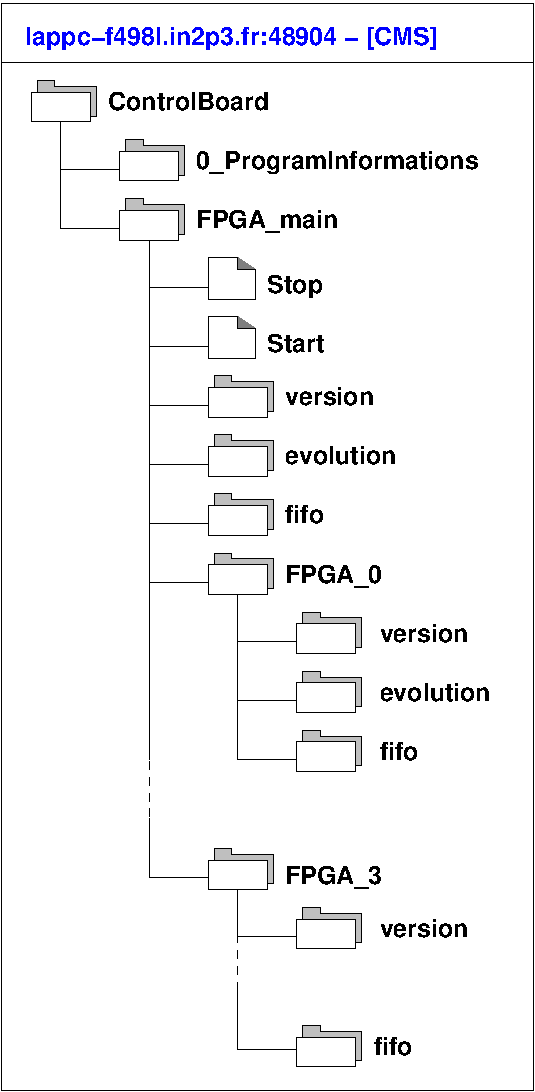
\includegraphics[width=5cm]{appendix/images/MOS_device_example_1.pdf}
\end{center}
\caption{Example of a  device managed through a MOS  server.  The root
  device is named \texttt{ControlBoard}.  First level daughter devices
  are  \texttt{0\_ProgramInformations} and  \texttt{FPGA\_main}.  Here
  the          MOS/OPCUA          server          is          labelled
  \texttt{CMS}.}\label{fig:an:mos_dev_1}
\end{figure}

% TODO


\subsection{Integration of a new device in the Vire environment}

The Vire  API also implements a  mechanism to describe a  hierarchy of
devices.  This  mechanism is independant  of the  one used in  the MOS
system but can  be easily made compatible with it.   This means that a
MOS  hierarchy  of devices  can  be  represented  in Vire.   The  Vire
hierarchy of  devices can  be considered as  some kind  of filesystem,
each device  being a folder with  its unique path, as  shown on figure
\ref{fig:an:mos_dev_2}.   The \emph{methods}  associated to  a devices
(or a datapoint) can be considered as plain executable files stored in
the  device's folder  : they  constitute the  set of  \emph{resources}
associated to the device.


\begin{figure}[h]
\begin{center}
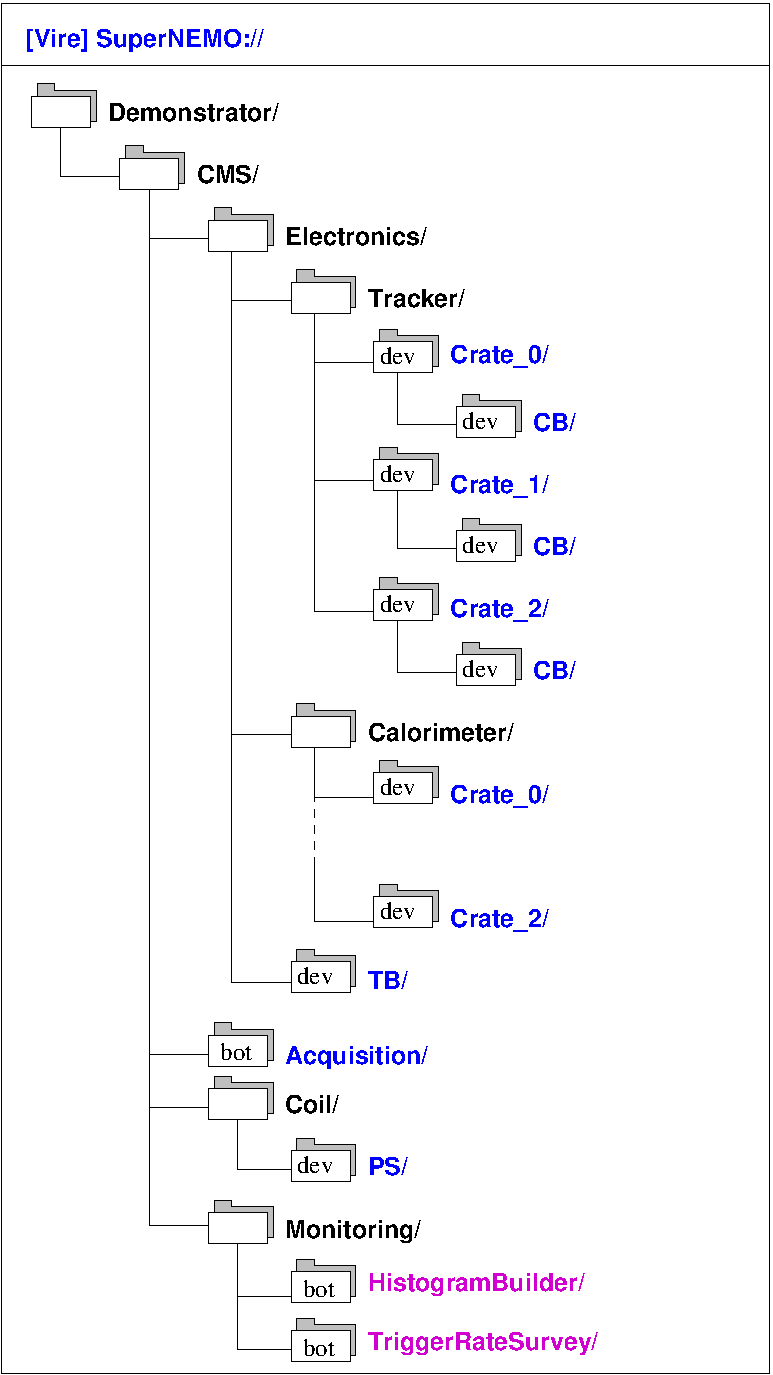
\includegraphics[width=5cm]{appendix/images/MOS_device_example_2.pdf}
\end{center}
\caption{Example of a hierarchy of  devices described by the Vire API.
  The root device is named  \texttt{SuperNEMO:}.  The top level (root)
  device  is  named  \texttt{Demonstrator}.  The  devices  colored  in
  \textcolor{blue}{blue}  are managed  through MOS/OPCUA.  The devices
  colored in \textcolor{magenta}{magenta} are directly embedded in the
  Vire server.  Devices with the \texttt{dev} tag are typical hardware
  device.  Devices  with the  \texttt{bot}  tag  are typical  software
  devices.   The  devices  colored in  \textbf{black}  are  structural
  pseudo-devices used to organize and  present a comprehensive view of
  the hierarchy. }\label{fig:an:mos_dev_2}
\end{figure}

The organisation of this hierarchy of devices is arbitrary and defined
by the designer of the  \emph{Control and Monitoring System}.  What is
important  to  understand  is  that  some  of  these  devices  can  be
associated  to  \emph{hardware  devices}  (a  power  supply  crate,  a
temperature probe\dots) and others  can be \emph{pseudo-devices}, i.e.
pure   software  object   (a   monitoring  robot,   a  file   transfer
daemon\dots).

In the context of the coupling of  the Vire server and the CMS server,
we are  in the event that  some devices are managed  by some MOS/OPCUA
servers and others are managed  in the Vire server itself.  Typically,
\emph{hardware devices}  are systematically managed through  the OPCUA
technology.  Vire has a mechanism to integrate such devices in its own
hierarchy.  This mechanism can  be considered like the \emph{mounting}
of   a   remote   filesystem   from  a   local   filesystem.    Figure
\ref{fig:an:mos_dev_0} illustrates  the case of many  hardware devices
-- managed by MOS -- that are integrated in the Vire system.  From the
Vire point of  view, the user does not see  the implementation details
for such  devices. He  does not  know the identity  of the  MOS server
hosting the device. He does not even know if the device is hosted by a
MOS server.  Devices are simply visible through the standard hierarchy
published by Vire with its  own device naming scheme, regardless their
true location.



\begin{figure}[h]
\begin{center}
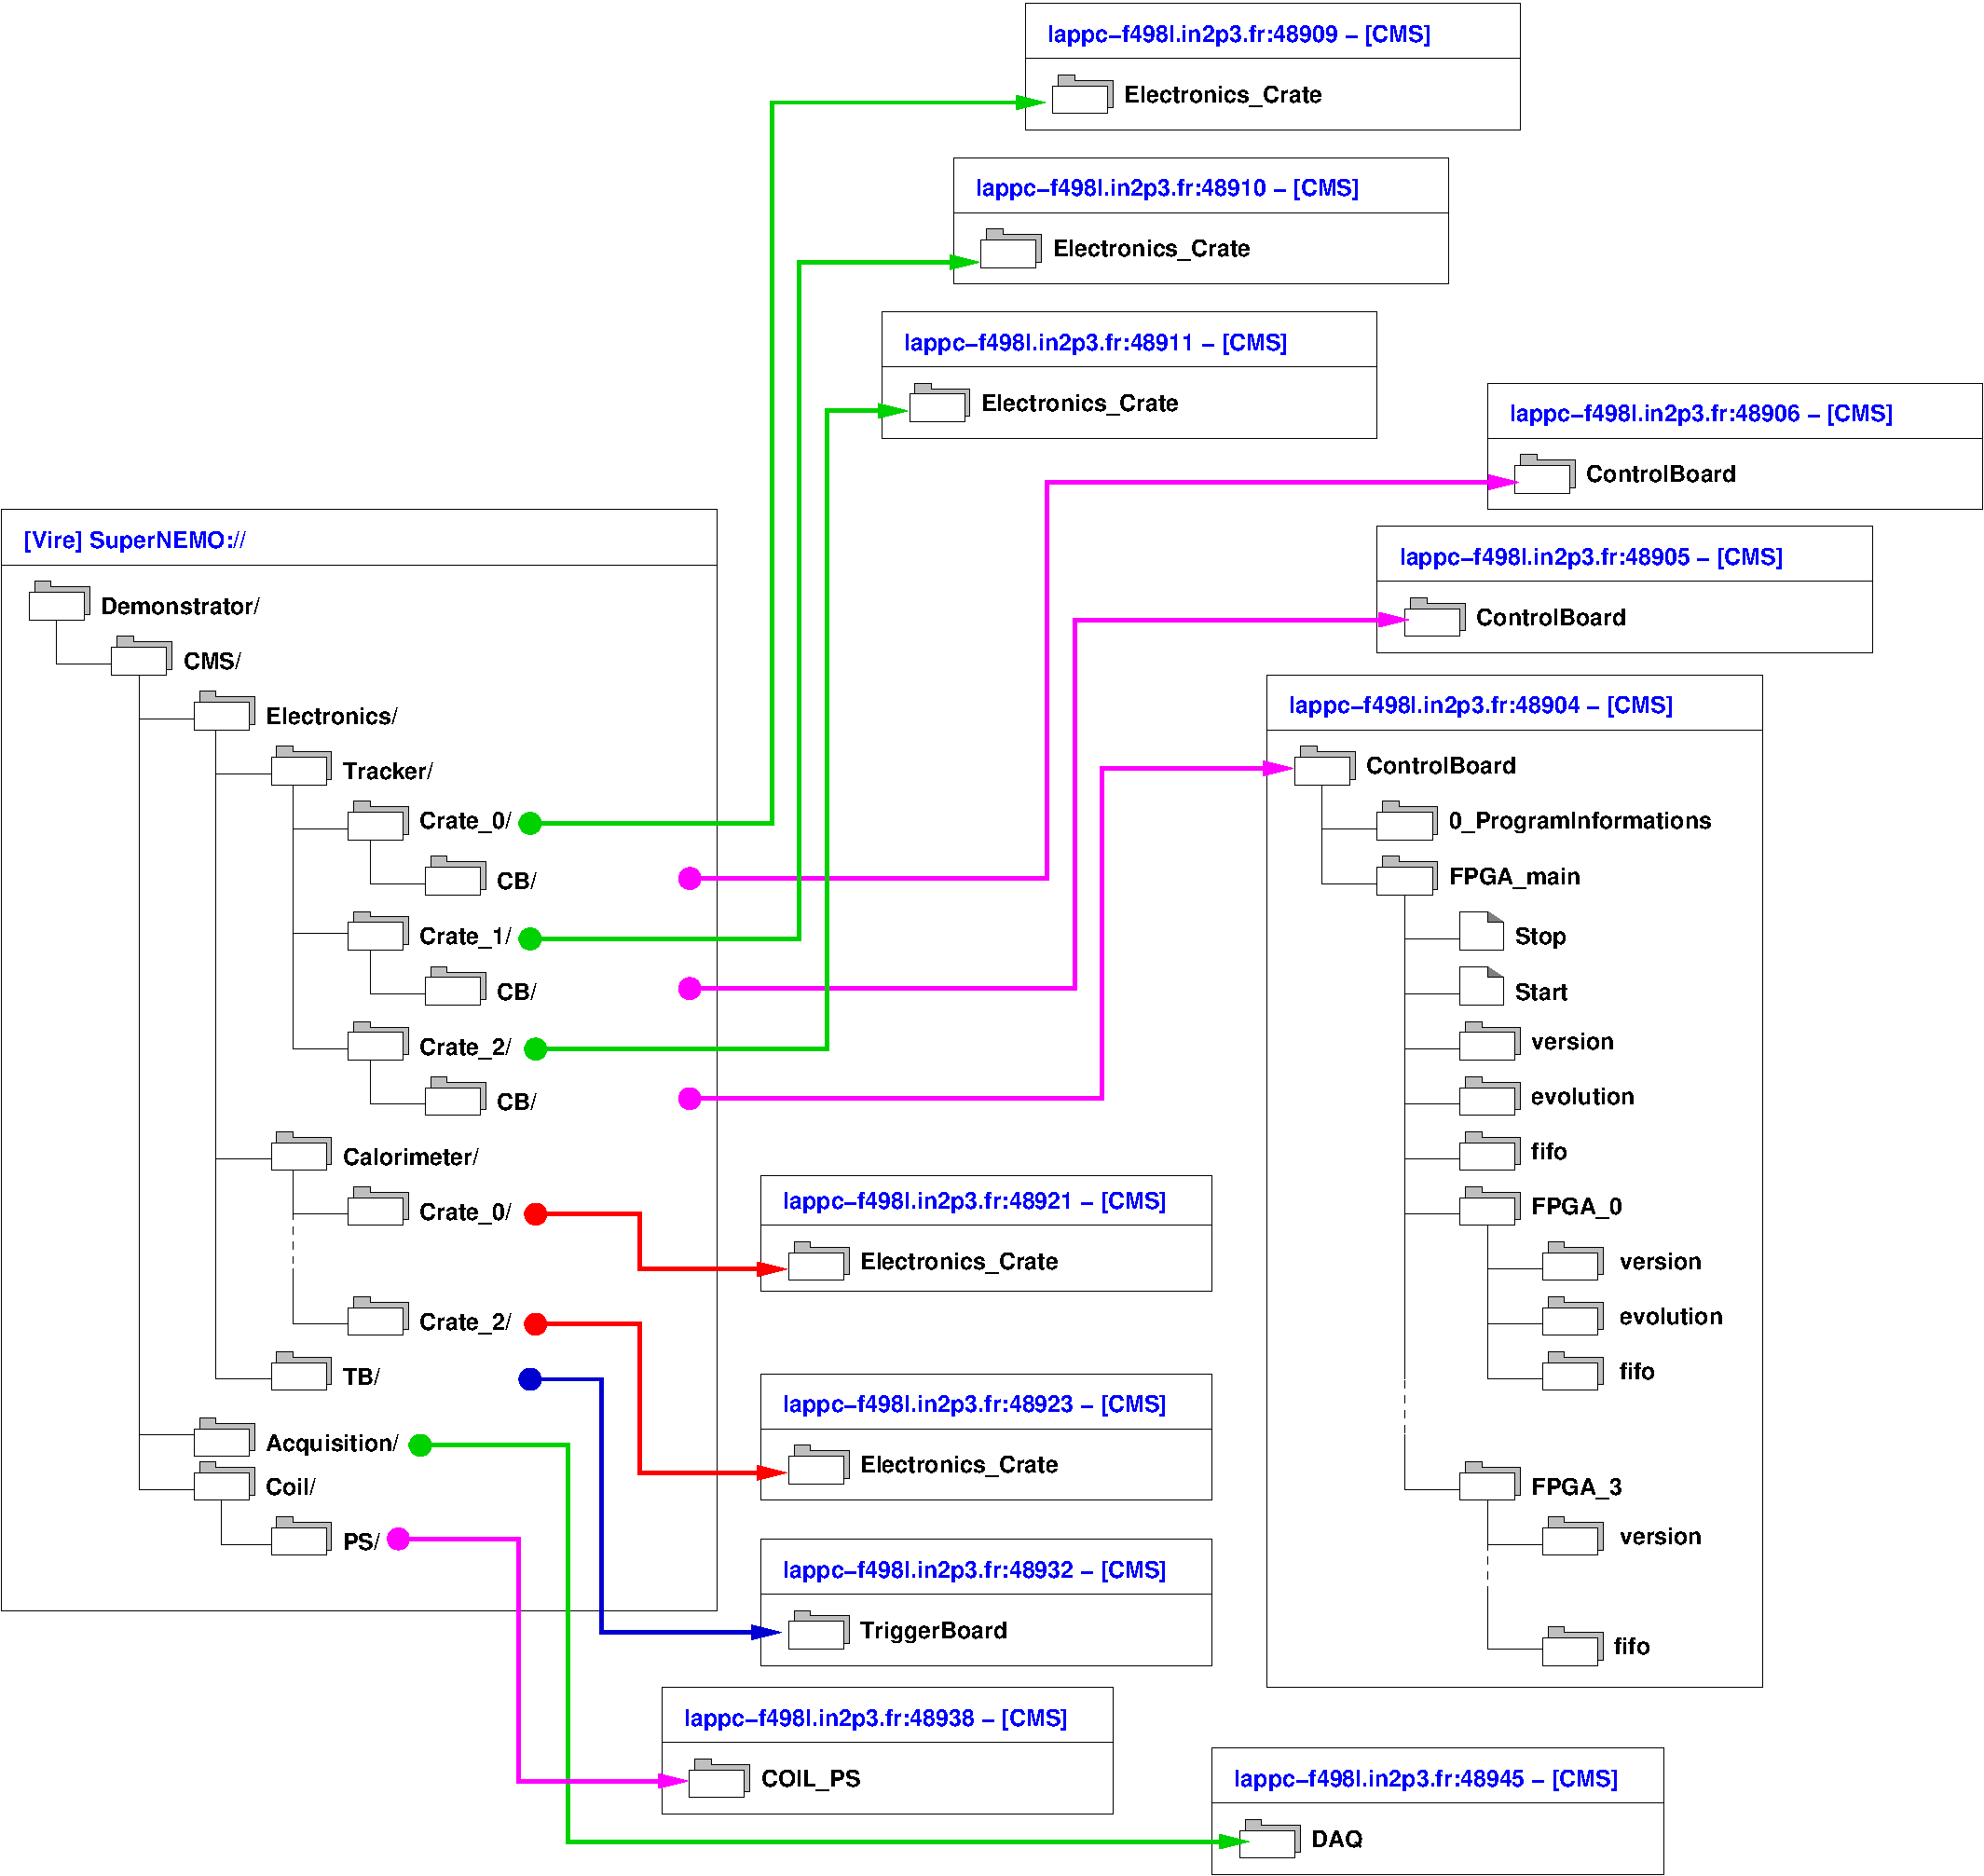
\includegraphics[width=\linewidth]{appendix/images/MOS_device_example_0.pdf}
\end{center}
\caption{The  mounting of  many  MOS device  hierarchies  in the  Vire
  device hierarchy.  Each OPCUA server  runs a simple  hardware device
  that is \emph{mounted} from a specific node with its own path.
%% of  devices described by the Vire API.
%%   The root device is named  \texttt{SuperNEMO:}.  The top level (root)
%%   device is  named \texttt{Demonstrator}. The devices  colored in blue
%%   are managed  through MOS/OPCUA. The  devices colored in  magenta are
%%   directly embedded in the Vire server.  Devices with the \texttt{dev}
%%   tag are typical  hardware device. Devices with  the \texttt{bot} tag
%%   are typical software devices.
}\label{fig:an:mos_dev_0}
\end{figure}




\subsection{Example}

Using  the examples  displayed  in  figure \ref{fig:an:mos_dev_0},  we
consider  in detail  the way  one specific  device managed  by MOS  is
mounted   in  the   Vire   hierarchy.  Figure   \ref{fig:an:mos_dev_3}
illustrates the mounting of a MOS device in Vire.

Here the Vire  server publishes the path of a  device representing the
control board  of the third  electronic crate  for the tracker  of the
SuperNEMO demonstrator module.  The full Vire path of this device is:

\textcolor{blue}{\texttt{SuperNEMO://Demonstrator/CMS/Electronics/Tracker/Crate\_2/CB}}

This is  the only Vire identifier  recognized by user to  address this
device.

On    the   figure,    one    can   see    that    the   MOS    server
\texttt{lappc−f498l.in2p3.fr} (port 48904) hosts a simple device which
is locally named \texttt{ControlBoard}.

When  mounting   this  device  in   the  Vire  hierarchy,   the  local
\texttt{[CMS]}  namespace and  \texttt{ControlBoard} device  names are
hidden and replaced by the Vire device path.  All daughter devices and
datapoints of  the \texttt{CMS/ControlBoard} device are  integrated as
daughters        of        the         Vire        device        named\\
\texttt{SuperNEMO://Demonstrator/CMS/Electronics/Tracker/Crate\_2/CB}.


For example, the \texttt{FPGA\_main} daughter device is now associated
to the following Vire path:

\textcolor{blue}{\texttt{SuperNEMO://Demonstrator/CMS/Electronics/Tracker/Crate\_2/CB/FPGA\_main/}}

and  its  \texttt{Stop} method  is  automatically  addressed with  the
following \emph{leaf} path:

\textcolor{blue}{\texttt{SuperNEMO://Demonstrator/CMS/Electronics/Tracker/Crate\_2/CB/FPGA\_main/Stop}}


\begin{figure}[h]
\begin{center}
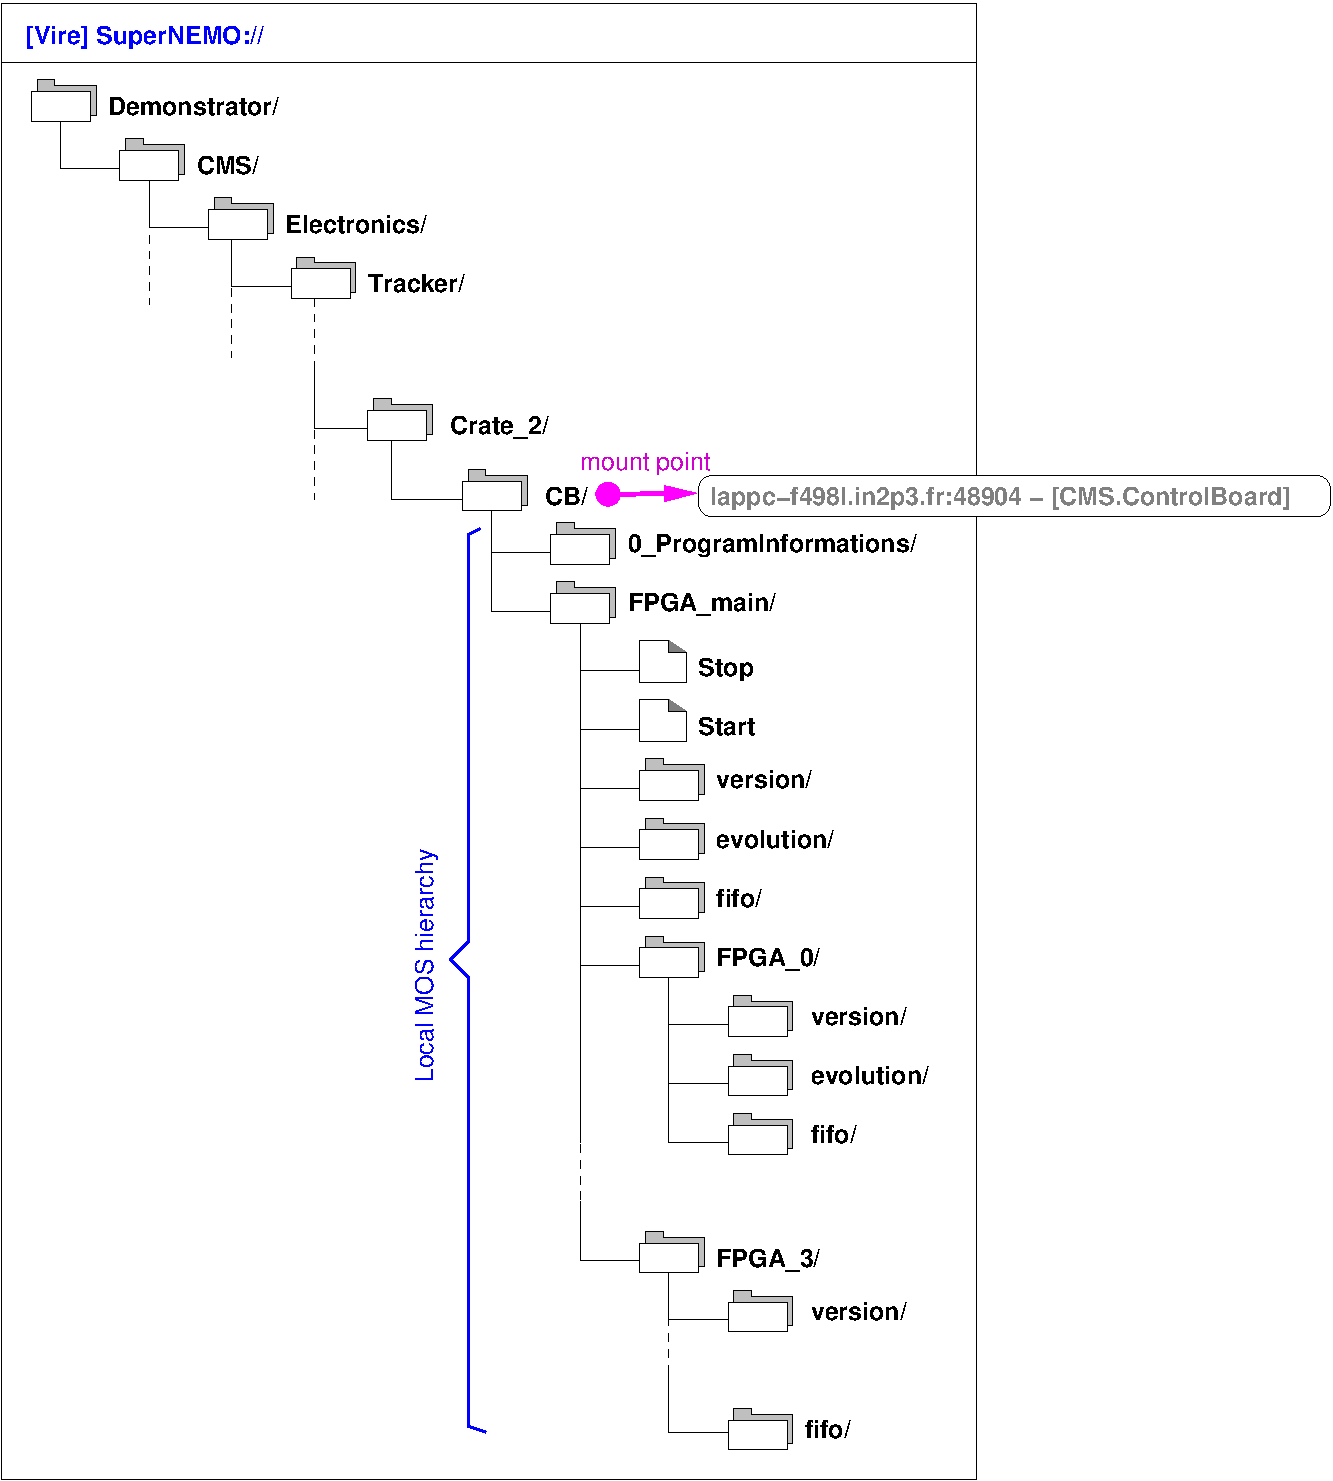
\includegraphics[width=0.8\linewidth]{appendix/images/MOS_device_example_3.pdf}
\end{center}
\caption{The  mounting of  one  MOS device and its local hierarchy  in the  Vire
  device hierarchy.}\label{fig:an:mos_dev_3}
\end{figure}



\subsection{Vire/MOS mapping}

As it can be  seen in the above example, the integration  of a new MOS
device in the Vire system is  achieved through soem kind of filesystem
mounting operation.   Particularly, it is  shown that the MOS  name of
the   mounted  root   device  is   replaced  by   an  arbitrary   Vire
path. However, all daughter  nodes (devices, datapoints) attached from
this root  node have their  relative MOS  names preserved in  the Vire
naming scheme.

Any  resource  (method)  associated  to any  of  such  daughter  nodes
inherits this relative naming scheme.

As Vire applications  describe resources through their  Vire paths, it
is thus needed to build an explicit map that associates resource paths
to MOS address  and name. The CMS  server will be able  to resolve the
MOS server/port and  embedded device associated to  the resource path.

The goal of the \texttt{devices\_launch.conf} file is not only to tell
the CMS server what MOS server should  be loaded and ran at start, but
also  to describe  the  \emph{mounting point/names}  used  by Vire  to
access the resources associated to MOS devices.  From the informations
stored in the  file, an explicit associative array must  be built when
the Vire server connect to the CMS server.  It will play the role of a
resource path resolver  when requests about resources will  be sent by
Vire applications.  This associative array  must be locked  during the
Vire/CMS connection.



%\subsubsection{Preparation of XML device models}

%% \noindent\underline{Pre-condition:}
%% The device is working and validated through the MOS/OPCUA server

%% \begin{enumerate}

%% \item Produce XML décrivant le modèle du device enrichi
%%   des metadata
%% Rédaction du fichier XML décrivant le modèle du device

%% \item Génération des fichiers model du type de device pour Vire

%% \item Génération des fichiers instances resolv.conf

%% \end{enumerate}


\vfill
\pagebreak
\clearpage

% end


\section{Vire messages}\label{app:vire_messages}

Within Vire  and between Vire  components and external  components, we
use  a communication  system  based on  Vire  messages.  This  section
describes the structure of such messages.

\subsection{General structure of a message}

Each message consists in two parts (figure \ref{fig-vire-message-message-cpp}):
\begin{itemize}

\item  the  \emph{header}  is   dedicated  to  generic  and  typicalle
  mandatory  informations  which  document   the  message  itself  and
  arbitrary high-level metadata.

\item  the \emph{body}  of the  message  contains the  real data: the payload.
  The structure of the message body depends on some convention. Vire uses
  its own convention to embed the payload data.

\end{itemize}

\begin{figure}[h]
\vskip 10pt
\small
\begin{Verbatim}[frame=single,xleftmargin=0.cm,label=\fbox{C++}]
struct vire::message::message {
  message_header header; // Header of the message
  message_body   body;   // Body of the message
};
\end{Verbatim}
\normalsize
\caption{The structure of a Vire message object (C++  class:
  \texttt{"vire::message::message"})}\label{fig-vire-message-message-cpp}
\end{figure}

\subsection{The message header}

The header contains (figure \ref{fig-vire-message-message_header-cpp}):
\begin{itemize}

  \item The mandatory \texttt{message\_id}  attribute is an identifier
    of the  message which  document the emitter  and a  unique message
    number.   Each emitter  is  responsible of  the  numbering of  the
    messages it  emits, typically using an  incremental technique. The
    message  number is  a positive  integer, starting  from 0  (figure
    \ref{fig-vire-message-message_identifier-cpp}).

  \item  The \texttt{timestamp}  attribute  encodes the  approximative
    time point when the message was  created. It contains the date and
    the time, using at least microsecond resolution.

    Typically,  with  JSON  encoding  system, it  is  expected  to  be
    formatted as a character string, using the following ISO format:

    \begin{center}
      \texttt{yyyymmddThhmmss.uuuuuu}
    \end{center}

    \noindent where:

    \vskip -10pt
    \begin{itemize}
    \item[\texttt{yyyymmdd} :] encodes year/month/day,
    \item[\texttt{hhmmssd} :] encodes hour/minute/second,
    \item[\texttt{uuuuuu} :] encodes microseconds.
    \end{itemize}

  \item   In   the   case    of   a   \emph{response}   message,   the
    \texttt{in\_reply\_to} attribute is set to identify the associated
    request message.

  \item  The \texttt{asynchronous}  boolean  attribute is  set if  the
    message processing  is explicitely requested  by the source  to be
    asynchronous (non-blocking).  In  RPC transactions, where requests
    are transmitted from one point to  the other, its default value is
    \emph{false}.   It  is possible  to  force  a RPC  transaction  in
    asynchronous mode.   This use  case is documented  elsewhere.  For
    event messaging, this flag is conventionally set to \emph{true}.

  \item  The  \texttt{body\_layout\_id}  attribute  is  the  mandatory
    identifier   of   the   layout   of  the   message   body   (class
    \texttt{"vire::utility::model\_identifier"}).  The  default layout
    for     message     body     inside    the     Vire     API     is
    \texttt{"vire::message::body\_format::typed\_payload"}, with version
    \texttt{"1.0"}                                             (figure
    \ref{fig-vire-utility-model_identifier-cpp}).

\end{itemize}


\begin{figure}[h]
\vskip 10pt
\small
\begin{Verbatim}[frame=single,xleftmargin=0.cm,label=\fbox{C++}]
struct vire::message::message_header {
  message_identifier message_id;     // Message identifier from the emitter.
  std::string        timestamp;      // Timestamp.
  message_identifier in_reply_to;    // Message identifier of the associated
                                     // request message (optional).
  bool               asynchronous,   // Asynchronous flag.
  vire::utility::model_identifier     body_layout_id; // Body layout identifier.
  std::map<std::string, std::string>  metadata;       // Key/value metadata dictionary.
};
\end{Verbatim}
\normalsize
\caption{The  structure  of  a   message  header  object  (C++  class:
  \texttt{"vire::message::message\_header"}).}\label{fig-vire-message-message_header-cpp}
\end{figure}

\begin{figure}[h]
\vskip 10pt
\small
\begin{Verbatim}[frame=single,xleftmargin=0.cm,label=\fbox{C++}]
struct vire::message::message_identifier {
  std::string emitter; // Name identifying the emitter of the message.
  int32_t     number;  // Number identifying the message in the emitter's
                       // message numbering scheme.
};
\end{Verbatim}
\normalsize
\caption{The      structure      of     a      message      identifier
  (C++  class:  \texttt{"vire::message::message\_identifier"}).}
\label{fig-vire-message-message_identifier-cpp}
\end{figure}

\begin{figure}[h]
\vskip 10pt
\small
\begin{Verbatim}[frame=single,xleftmargin=0.cm,label=\fbox{C++}]
struct vire::utility::model_identifier {
  std::string name;    // Name identifying the format of the message.
  std::string version; // String identifying the version of the format.
};
\end{Verbatim}
\normalsize
\caption{The structure of a model identifier (C++  class:  \texttt{"vire::utility::model\_identifier"}.}\label{fig-vire-utility-model_identifier-cpp}
\end{figure}




\begin{figure}[h]
\vskip 10pt
\small
\begin{Verbatim}[frame=single,xleftmargin=0.cm,label=\fbox{JSON}]
{
   "header" : {
      "message_id" : {
         "emitter" : "vire.server",
         "number" : 42
      },
      "timestamp" : "20160930T141408.413443",
      "in_reply_to" : {
         "initialized" : true,
         "value" : {
            "emitter" : "vire.client.0",
            "number" : 23
         }
      },
      "asynchronous" : false,
      "body_layout_id" : {
         "name" : "vire::message::body_format::typed_payload",
         "version" : {
            "initialized" : true,
            "value" : "1.0"
         }
      },
      "metadata" : [
         {
            "key" : "key1",
            "value" : "foo"
         },
         {
            "key" : "key2",
            "value" : "42"
         },
         {
            "key" : "key3",
            "value" : "3.1415899999999999"
         },
         {
            "key" : "key4",
            "value" : "true"
         }
      ]
   }
  "body" : {
      ...
   }
}
\end{Verbatim}
\normalsize
\caption{Example of  a   message  header  object in JSON format.}
\label{fig-vire-message-message_header-json}
\end{figure}

\vfill
\clearpage
\pagebreak

\subsection{The message body}

The    default    message   body    layout    in    Vire   is    named
\texttt{"vire::message::body\_format::typed\_payload"}        (version
\texttt{"1.0"}).   Each  message used  within  the  Vire framework  is
supposed to use this layout.  The general idea is that the body of the
message embeded the  \emph{payload object} that has  to be transmitted
between  two components  of  the system.   \emph{Payload objects}  are
classified in one of the three following categories:

\begin{enumerate}

\item \emph{Request}:  describes a request submitted  by one component
  to another component (generally during a synchronous RPC transaction).

\item  \emph{Response}: describes  the  response to  a former  request
  (generally during a synchronous RPC transaction).

\item \emph{Event}: describes an  arbitrary information record (alarm,
  exception, signal\dots) which is transmitted asynchronously.

\end{enumerate}

Vire implements the following class hierarchy:

\begin{center}
\begin{tikzpicture}
  \node (payload)  at (0,2)  [draw] {\texttt{vire::utility::base\_payload}};
  \node (request)  at (-4,0) [draw] {\texttt{vire::utility::base\_request}};
  \node (response) at (2,0)  [draw] {\texttt{vire::utility::base\_response}};
  \node (event)    at (8,0)  [draw] {\texttt{vire::utility::base\_event}};

  %\draw[style=help lines] (-3,-1) grid (10,4);
  \draw (node cs:name=response,anchor=north) |- (0,1);
  \draw (node cs:name=event,anchor=north)    |- (0,1);
  \draw[->] (node cs:name=request,anchor=north)
  |- (0,1) -| (node cs:name=payload,anchor=south);
\end{tikzpicture}
\end{center}

The requirements for the transmitted object are the following:

\begin{itemize}

\item The  type of the object  must be conventionally associated  to a
  unique     \emph{model      identifier}     object      (see     the
  \texttt{"vire::utility::model\_identifier"} class)  which contains a
  unique   name   (\textit{string    identifier})   and   possibly   a
  \textit{version identifier}.  Each software  component that may send
  or  receive the  object  should agree  on  this type  identification
  scheme.   This   enable  the  use  of   object  factories,  whatever
  programming  langage  is used  on  both  side of  the  communication
  system.

\item  For each  software component,  the object  type must  have some
  dedicated  encoding/decoding  functions  available  (again  whatever
  programming language is used). For example the Vire API supports the
  following encoding formats:

  \begin{itemize}

  \item JSON (MIME  encoding type: \texttt{"application/x-json"}), which
    is supportable by many languages,

  \item  Protobuf  (Google  Protocol   Buffers,  MIME  encoding  type:
    \texttt{"application/x-protobuf"}), which is also widely supported,

  \item   Boost/serialisation   (XML,    text   or   binary   archives
    \texttt{"application/x-boost-serialization-xml"},
    \texttt{"application/x-boost-serialization-text"},
    \texttt{"application/x-boost-serialization-binary"}),    which    in
    principle is supported by C++ only.

  \end{itemize}

  The Protobuf  encoding format will be  used to serialize/deserialize
  the  Vire  messages transported  between  the  Vire server  and  the
  CMS/LAPP server.

\end{itemize}

Vire uses a dedicated layout to represent the body of any message with
its embedded payload object. With this technique, the structure of the
body          contains         two          attributes         (figure
\ref{fig-app-vire-message-message_body-cpp}):

\begin{enumerate}

\item The \texttt{payload\_type\_id} specifies the type of the payload
  object   (figure   \ref{fig-app-vire-utility-model_identifier-cpp}).
  This unique name  is conventionaly fixed for a  given application. A
  version tag allows to support possible evolution of the object type.

\item The  \texttt{payload} is a  handle to  a payload object  of type
  request, response or event.

  %% \begin{itemize}
  %% \item Within  the producer  component of  the message,  the encoding
  %%   function associated to the object  type is responsible to generate
  %%   the JSON stream for the object and store it in the buffer.

  %% \item Within  the consumer  component of  the message,  the decoding
  %%   function associated to the object type is responsible to parse the
  %%   JSON stream stored in the buffer and restore the object in memory.

  %% \end{itemize}

  It is expected  that, on both sides of the  connection, the software
  components can  access dedicated  software plugins which  ensure the
  support  of  various   \emph{payload  object  types}  conventionnaly
  associated  with  their  \emph{payload type  identifiers}  and  also
  providing JSON and/or Protobuf encoding/decoding functionalities.

  %% The   system  allows  to  support
  %% modification  in the  structure of  the objects  thanks to  version
  %% tagging.

\end{enumerate}

\begin{figure}[h]
\vskip 10pt
\small
\begin{Verbatim}[frame=single,xleftmargin=0.cm,label=\fbox{C++}]
struct message_body {
  vire::utility::model_identifier     payload_type_id; // Object type identifier.
  const vire::utility::base_payload * payload;         // Handle to a payload object.
};
\end{Verbatim}
\normalsize
\caption{The structure of a message body object (C++).}
\label{fig-app-vire-message-message_body-cpp}
\end{figure}

\begin{figure}[h]
\vskip 10pt
\small
\begin{Verbatim}[frame=single,xleftmargin=0.cm,label=\fbox{JSON}]
{
  "header" : {
    ...
  },
  "body" : {
    "payload_type_id" : {
      "name" : "vire::message::testing::error_event",
      "version" : {
        "initialized" : false
      }
    },
    "payload" : {
      "timestamp" : "20160930T141743.759085"
      "err" : {
        "code" : 3,
        "message" : "A basic error"
      },
    }
  }
}
\end{Verbatim}
\normalsize
\caption{Example of  a   message  body  object in JSON format.}
\label{fig-vire-message-message_body-json}
\end{figure}

\vfill
\clearpage
\pagebreak

% end

%\input{appendix/app_json_fmt.tex}

\section{The \emph{Protocol Buffers} format}\label{app:protobuf_fmt}

\subsection{Introduction}

The  Google  Protocol Buffers  (\emph{protobuf})  library  is used  to
represent the objects that are exchanged between the Vire clients, the
Vire server and the CMS server.  The  version 3 of the format is used,
implying   at   least   version   3.0.0  (September   2016)   of   the
\emph{protobuf} library.

Each  data   structure  of  interest   can  be  described   through  a
\texttt{.proto}  file  from  which  stub files  can  be  automatically
generated  with the  \texttt{protoc} compiler.  For Vire  and its  CMS
interface, the C++ and Java programming languages will be used.


A  collection of  \texttt{.proto}  files are  provided  with the  Vire
library to represent all kind  of data structures transferable between
networked agents  (Vire server,  Vire clients, CMS/LAPP  server).  The
objects of  the highest level  are named \emph{payload  objects} (like
\emph{request},  \emph{response} and  \emph{event} objects).   They
are composed of attributes of more basic data structures.

\subsection{Example}

The following  class diagram  illustrates two data  structures defined
within the Vire library with an inheritance relationship between them.

\begin{center}
  \begin{tikzpicture}
    \node (base)     at (0,1.5)  [draw] {\texttt{vire::utility::base\_error}};
    \node (setup)    at (0,0)  [draw] {\texttt{vire::utility::invalid\_setup\_id\_error}};

    \draw[->]   (node cs:name=setup,anchor=north) |- (0,1);
    |- (0,1) -| (node cs:name=base,anchor=south);
  \end{tikzpicture}
\end{center}

The \texttt{vire::utility::base\_error}  is the  parent class  for all
\emph{error}  objects.   It  contains   two  attributes:   an  integer
\emph{error code}  and a  character string describing  the \emph{error
  message}.

The   \texttt{vire::utility::invalid\_setup\_id\_error}  class   is  a
specialized error class  which represents explicitely an  error due to
an identification  failure of  the experimental setup.   It implements
additional mutually exclusive attributes: the \emph{unrecognized name}
of the setup or the \emph{unrecognized version} of the setup.

This   example  illustrates   the  protobuf   representation  of   the
\texttt{vire::utility::base\_error}  in the  Vire  library, using  the
\texttt{"vire/utility/BaseError.proto"} file:

\small
\begin{Verbatim}[frame=single,xleftmargin=0.cm,label=\fbox{protobuf}]
  syntax = "proto3";
  package vire.utility; // Namespace

  message BaseError {

    // reserved 1; // Reserved for _base message

    // Attributes:
    int32  code           = 100; // The error code
    string message_format = 101; // The error description message

  }
\end{Verbatim}
\normalsize

\vfill
\clearpage
\pagebreak

\subsection{Vire protobuf conventions}

Vire uses the following conventions:

\begin{enumerate}

\item
  The member index  \texttt{1} is reserved to represent the  link of a
  class to its main base/parent class (if any).  It is not used if the
  data structure does not inherit any data structure.
  If a data structure naturally inherits another one, it is thus possible
  to  represent the  inheritance  relationship as  illustrated with  the
  \texttt{"vire/utility/InvalidSetupIdError.proto"}      file      which
  represents the \texttt{vire::utility::invalid\_setup\_id\_error} class
  in the Vire library:

  \small
  \begin{Verbatim}[frame=single,xleftmargin=0.cm,label=\fbox{protobuf}]
    syntax = "proto3";
    package vire.utility; // Namespace

    import "vire/utility/BaseError.proto"; // Dependency

    message InvalidSetupIdError {

      BaseError _base = 1; // The base class

      // Additional attributes:
      oneof detail { // Mutual exclusion
        string invalid_setup_name    = 100; // The failed setup name
        string invalid_setup_version = 101; // The failed setup version
      }

    }
  \end{Verbatim}
  \normalsize

\item The  \texttt{\_base} member  is conventionally  used to  represent the
  inheritance   relationship    from   a   data   structure    of   type
  \texttt{"vire.utility.BaseError"}.

\item Member indexes from \texttt{2}  to \texttt{99} are also reserved
  for possible future usage (multiple inheritance, metadata\dots).

\item
  The first member of the data structure must start at index \texttt{100}.

\end{enumerate}

\vfill
\clearpage
\pagebreak

% end


\section{Vire payload objects}\label{app:payload}

\subsection{Introduction}

As  mentioned in  appendix \ref{app:protobuf_fmt},  Vire messages  are
wrappers for \emph{payload objects}.  Each  type of payload object can
be represented  through the \emph{protobuf} mechanism.   The following
class hierarchy shows the base architecture used to define new payload
objects.

\begin{center}
\begin{tikzpicture}
  \node (payload)  at (0,2)   [draw] {\texttt{vire::utility::base\_payload}};
  \node (request)  at (-4,0)  [draw] {\texttt{vire::utility::base\_request}};
  \node (response) at (2,0)   [draw] {\texttt{vire::utility::base\_response}};
  \node (event)    at (8,0)   [draw] {\texttt{vire::utility::base\_event}};
  \node (my)       at (-4,-2) [draw] {\texttt{my\_request}};
  \node (your)     at (2,-2)  [draw] {\texttt{your\_response}};
  \node (its)    at (8,-2)    [draw] {\texttt{its\_alarm}};

  %\draw[style=help lines] (-6,-2) grid (10,2);
  \draw (node cs:name=response,anchor=north) |- (0,1);
  \draw (node cs:name=event,anchor=north)    |- (0,1);
  \draw[->] (node cs:name=request,anchor=north)
  |- (0,1) -| (node cs:name=payload,anchor=south);
  \draw[->] (node cs:name=my,anchor=north)
  |- (-4,-1) -| (node cs:name=request,anchor=south);
  \draw[->] (node cs:name=your,anchor=north)
  |- (2,-1) -| (node cs:name=response,anchor=south);
  \draw[->] (node cs:name=its,anchor=north)
  |- (8,-1) -| (node cs:name=event,anchor=south);
\end{tikzpicture}
\end{center}


\begin{center}
\vskip 10pt
\small
\begin{tabular}{|l|l|l|}
  \hline
  \textbf{Vire C++ class} & \textbf{protobuf message type} & \textbf{protobuf definition file} \\
  \hline
  \hline
  \multicolumn{3}{|c|}{\emph{general types}} \\
  \hline
  boost::posix\_time::ptime & google.protobuf.Timestamp & google/protobuf/timestamp.proto \\
  \hline
  \hline
  \multicolumn{3}{|c|}{\emph{identifier types}} \\
  \hline
  vire::utility::base\_identifier & vire.utility.Baseidentifier & vire/utility/Baseidentifier.proto \\
  \hline
  vire::utility::instance\_identifier & vire.utility.InstanceIdentifier & vire/utility/InstanceIdentifier.proto \\
  \hline
  vire::utility::model\_identifier & vire.utility.ModelIdentifier & vire/utility/ModelIdentifier.proto \\
  \hline
  \hline
  \multicolumn{3}{|c|}{\emph{error types}} \\
  \hline
  vire::utility::base\_error & vire.utility.BaseError & vire/utility/BaseError.proto \\
  \hline
  vire::utility::invalid\_context\_error & vire.utility.InvalidContextError & vire/utility/InvalidContextError.proto \\
  \hline
  vire::utility::invalid\_setup\_id\_error & vire.utility.InvalidSetupIdError & vire/utility/InvalidSetupIdError.proto \\
  \hline
  \hline
  \multicolumn{3}{|c|}{\emph{payload types}} \\
  \hline
  vire::utility::base\_payload & vire.utility.BasePayload & vire/utility/BasePayload.proto \\
  \hline
  vire::utility::base\_request & vire.utility.BaseRequest & vire/utility/BaseRequest.proto \\
  \hline
  vire::utility::base\_response & vire.utility.BaseResponse & vire/utility/BaseResponse.proto \\
  \hline
  vire::utility::base\_event & vire.utility.BaseEvent & vire/utility/BaseEvent.proto \\
  \hline
  vire::utility::base\_alarm & vire.utility.BaseAlarm & vire/utility/BaseAlarm.proto \\
  \hline
  \hline
  \multicolumn{3}{|c|}{\emph{messenging types}} \\
  \hline
  vire::message::message\_identifier & vire.message.MessageIdentifier & vire/message/MessageIdentifier.proto \\
  \hline
  vire::message::msg\_header & vire.message.MsgHeader & vire/message/MsgHeader.proto \\
  \hline
  vire::message::msg\_body & vire.message.MsgBody & vire/message/MsgBody.proto \\
  \hline
  vire::message::message & vire.message.Message & vire/message/Message.proto \\
  \hline
\end{tabular}
\normalsize
\end{center}


\begin{center}
\vskip 10pt
\small
\begin{tabular}{|l|l|l|}
  \hline
  \multicolumn{3}{|c|}{\emph{Resource management related types}} \\
  \hline
  vire::cms::resource\_status\_record & vire.cms.ResourceStatusRecord & vire/cms/ResourceStatusRecord.proto \\
  \hline
  vire::cms::resource\_fetch\_status\_request & vire.cms.ResourceFetchStatusRequest & vire/cms/ResourceFetchStatusRequest.proto \\
  \hline
  vire::cms::resource\_fetch\_status\_success\_response & vire.cms.ResourceFetchStatusSuccessResponse & vire/cms/ResourceFetchStatusSuccessResponse.proto \\
  \hline
  vire::cms::resource\_fetch\_status\_failure\_response & vire.cms.ResourceFetchStatusFailureResponse & vire/cms/ResourceFetchStatusFailureResponse.proto \\
  \hline
  vire::cms::resource\_exec\_request & vire.cms.ResourceExecRequest & vire/cms/ResourceExecRequest.proto \\
  \hline
  vire::cms::resource\_exec\_success\_response & vire.cms.ResourceExecSuccessResponse & vire/cms/ResourceExecSuccessResponse.proto \\
  \hline
  vire::cms::resource\_exec\_failure\_response & vire.cms.ResourceExecFailureResponse & vire/cms/ResourceExecFailureResponse.proto \\
  \hline
  vire::cms::resource\_exec\_non\_blocking\_request & vire.cms.ResourceExecNonBlockingRequest & vire/cms/ResourceExecNonBlockingRequest.proto \\
  \hline
  vire::cms::resource\_exec\_non\_blocking\_ack\_response & vire.cms.ResourceExecNonBlockingAckResponse & vire/cms/ResourceExecNonBlockingAckResponse.proto \\
  \hline
  vire::cms::resource\_exec\_non\_blocking\_noack\_response & vire.cms.ResourceExecNonBlockingNoackResponse & vire/cms/ResourceExecNonBlockingNoackResponse.proto \\
  \hline
  vire::cms::resource\_exec\_non\_blocking\_success\_event & vire.cms.ResourceExecNonBlockingSuccessEvent & vire/cms/ResourceExecNonBlockingSuccessEvent.proto \\
  \hline
  vire::cms::resource\_exec\_non\_blocking\_failure\_event & vire.cms.ResourceExecNonBlockingFailureEvent & vire/cms/ResourceExecNonBlockingFailureEvent.proto \\
  \hline
  vire::cms::resource\_exec\_error & vire.cms.ResourceExecError & vire/cms/ResourceExecError.proto \\
  \hline
  vire::cms::invalid\_status\_error & vire.cms.ResourceExecError & vire/cms/ResourceExecError.proto \\
  \hline
  %% vire::cms::invalid\_credentials\_error & vire.cms.InvalidCredentialsError & vire/cms/InvalidCredentialsError.proto \\
  %% \hline
  %% vire::cms::invalid\_user\_error & vire.cms.InvalidUserError & vire/cms/InvalidUserError.proto \\
  %% \hline
  vire::cms::invalid\_resource\_error & vire.cms.InvalidUserError & vire/cms/InvalidUserError.proto \\
  \hline
  vire::cms::no\_pubsub\_resource\_error & vire.cms.NoPubsubResourceError & vire/cms/NoPubsubResourceError.proto \\
  \hline
  \hline
  \multicolumn{3}{|c|}{\emph{Resource pub/sub management types}} \\
  \hline
  vire::cms::resource\_pubsub\_subscribe\_request & vire.cms.ResourcePubsubSubscribeRequest & vire/cms/ResourcePubsubSubscribeRequest.proto \\
  \hline
  vire::cms::resource\_pubsub\_subscribe\_success\_response & vire.cms.ResourcePubsubSubscribeRSuccessResponse & vire/cms/ResourcePubsubSubscribeRSuccessResponse.proto \\
  \hline
  vire::cms::resource\_pubsub\_subscribe\_failure\_response & vire.cms.ResourcePubsubSubscribeRFailureResponse & vire/cms/ResourcePubsubSubscribeRSuccessResponse.proto \\
  \hline
  \hline
  \multicolumn{3}{|c|}{\emph{Vire/CMS server interface types}} \\
  \hline
  vire::cmsinterface::connection\_request & vire.cmsinterface.ConnectionRequest & vire/cmsinterface/ConnectionRequest.proto \\
  \hline
  vire::cmsinterface::connection\_success\_response & vire.cmsinterface.ConnectionSuccessResponse & vire/cmsinterface/ConnectionSuccessResponse.proto \\
  \hline
  vire::cmsinterface::connection\_failure\_response & vire.cmsinterface.ConnectionFailureResponse & vire/cmsinterface/ConnectionFailureResponse.proto \\
  \emph{embedded:} unknown\_resources\_error & .UnknownResourcesError &  \\
  \hline
  vire::cmsinterface::disconnection\_request & vire.cmsinterface.DisconnectionRequest & vire/cmsinterface/DisconnectionRequest.proto \\
  \hline
  vire::cmsinterface::disconnection\_success\_response & vire.cmsinterface.DisconnectionSuccessResponse & vire/cmsinterface/DisconnectionSuccessResponse.proto \\
  \hline
  %% \hline
  %% vire::cmsinterface::disconnection\_failure\_response & vire.cmsinterface.DisconnectionFailureResponse & vire/cmsinterface/DisconnectionFailureResponse.proto \\
\end{tabular}
\normalsize
\end{center}

\subsection{Basic data structures}

Any  payload object  (request, response  or event)  generally contains
some information records which are  specific to the functionalities of
the  payload  object they  belong.   These  records are  of  arbitrary
types. Of course they should be  translatable in terms of the protobuf
library.
%Of course they can be (de)serialized using JSON.
Some of these types are very  general and defined within the Vire core
API itself because they are reused by various payload objects not only
through  the Vire-CMS/LAPP  interface  but also  between  Vire clients  and
servers, independently  of the  CMS/LAPP server.  However,  the use  of the
Protocol Buffers interface makes possible  to publish the interface of
such data to the outside world, including the CMS/LAPP server in priority.

%% Other one are specific to the Vire/CMS interface and thus managed only
%% in the \texttt{Vire\_CMSInterface} API.
These  types  are considered  as  \emph{basic}.  Among them  we  find:
generic error  types, generic  identifier types,  timestamps, resource
status records\dots We propose to describe them in this section.

Once a sufficient collection of  basic data record types is available,
it  is possible  to describe  high  level payload  object types  which
aggregate attributes of such types.

Other record  types are specific to  some payload objects and  will be
never  used outside  the scope  of these  payload objects.   Such data
structures will be  explicitely declared with the  payload object they
belong to, likely as embedded types/classes.


\subsubsection{Errors}

Some  \emph{response} or  \emph{event} payload  objects may  contain a
specific  error  record  object.   A  \emph{failure  response}  or  an
\emph{exception  event}  object will  generally  embed  such an  error
record object.

Each  \emph{error record}  is represented  by an  instance of  a given
error type.   Each of  the error  types defined  in Vire  inherits the
\texttt{vire::utility::base\_error}      base       class      (figure
\ref{fig-app-payload-base_error})   which   contains   the   following
attributes:

\begin{itemize}

\item the error code: A non zero  integer which is set to 1 by default
  (indicating  a  generic  failure  case).   The  error  code  can  be
  conventionally  set to  any positive  integer value  to represent  a
  specific error case, depending on the context.

\item the error  message: an optional human  readable character string
  which documents the error as usefully as possible.

\end{itemize}

\begin{figure}[h]
\vskip 10pt
\small
\begin{Verbatim}[frame=single,xleftmargin=0.cm,label=\fbox{C++}]
struct vire::utility::base_error
{
  // Attributes:
  int         code;           // Error code (>0).
  std::string message_format; // Error message (optional).
};
\end{Verbatim}
\normalsize
\caption{The structure of a \texttt{"vire::utility::base\_error"} object
  (C++).}
\label{fig-app-payload-base_error}
\end{figure}


%% An example of JSON formatted basic error object is given in figure
%% \ref{fig-app-payload-base_error-1}.
%%
%% \begin{figure}[h]
%% \vskip 10pt
%% \small
%% \begin{Verbatim}[frame=single,xleftmargin=0.cm,label=\fbox{\texttt{JSON}}]
%% {
%%   "code" : "42",
%%   "message_format" : "Invalid AMQP server port=[2341]"
%% }
%% \end{Verbatim}
%% \normalsize
%% \caption{JSON  formatted  basic  error  object  (class
%%   \texttt{vire::utility::base\_error}.}
%% \label{fig-app-payload-base_error-1}
%% \end{figure}

Several type of generic errors are defined in Vire:


\begin{center}
\begin{tikzpicture}
  \node (base)     at (0,2)  [draw] {\texttt{vire::utility::base\_error}};
  \node (context)  at (-4,0) [draw] {\texttt{vire::utility::invalid\_context\_error}};
  \node (setup)    at (0,-1)  [draw] {\texttt{vire::utility::invalid\_setup\_id\_error}};
  \node (resource) at (4,0)  [draw] {\texttt{vire::cms::invalid\_resource\_error}};
  \node (user)     at (8,-1)  [draw] {\texttt{vire::cms::invalid\_user\_error}};

  \draw     (node cs:name=setup,anchor=north)    |- (0,1);
  \draw     (node cs:name=resource,anchor=north) |- (0,1);
  \draw     (node cs:name=user,anchor=north)     |- (0,1);
  \draw[->] (node cs:name=context,anchor=north)
  |- (0,1) -| (node cs:name=base,anchor=south);
\end{tikzpicture}
\end{center}

\noindent
Here are a few error object types defined in Vire.  Some types belongs
to the \texttt{utility} namespace, other  ones are in the \texttt{cms}
namespace:

\begin{itemize}

\item \texttt{"vire::utility::invalid\_context\_error"} : occurs typically when
  the general context of the execution of a given resource is not adapted.\\
  It is mapped to the \texttt{"vire.utility.InvalidContextError"} protobuf record.

\item \texttt{"vire::utility::invalid\_setup\_id\_error"} : occurs in case
  of an invalid identification of the experimental setup managed
  by the Vire or CMS server.\\
  It is mapped to the \texttt{"vire.utility.InvalidSetupIdError"} protobuf record.

\item \texttt{"vire::cms::invalid\_resource\_error"} : occurs in case
  of an invalid identification of a resource.\\
  It is mapped to the  \texttt{"vire.cms.InvalidResourceError"} protobuf record.

\item \texttt{"vire::cms::invalid\_status\_error"}: occurs when an attempt
  to access a resource that has not the proper status.\\
  It is mapped to the  \texttt{"vire.cms.InvalidStatusError"} protobuf record.

\item \texttt{"vire::cms::invalid\_user\_error"} : occurs in case
  of an invalid identification of an user.\\
  It is mapped to the  \texttt{"vire.cms.InvalidUserError"} protobuf record.

\item \texttt{"vire::cms::invalid\_credentials\_error"} : occurs in case
  of user authentication error.\\
  It is mapped to the  \texttt{"vire.cms.InvalidCredentialsError"} protobuf record.

\item \texttt{"vire::cms::resource\_exec\_error"} : occurs in case
  of error at the execution of a given resource.\\
  It is mapped to the  \texttt{"vire.cms.ResourceExecError"} protobuf record.

\end{itemize}



\subsubsection{Object and type identifiers}

Vire  uses  some dedicated  classes  to  represent the  identifier  of
various objects  (or \emph{instances})  as well  as various  types (or
\emph{models})  of components.  Vire  implements  the following  class
hierarchy:

\begin{center}
\begin{tikzpicture}
  \node (base)  at (0,2)  [draw] {\texttt{vire::utility::base\_identifier}};
  \node (instance)  at (-4,0) [draw] {\texttt{vire::utility::instance\_identifier}};
  \node (model) at (4,0)  [draw] {\texttt{vire::utility::model\_identifier}};

  \draw (node cs:name=model,anchor=north) |- (0,1);
\draw[->] (node cs:name=instance,anchor=north)
  |- (0,1) -| (node cs:name=base,anchor=south);
\end{tikzpicture}
\end{center}

The          \texttt{vire::utility::base\_identifier}          (figure
\ref{fig-app-payload-base_identifier}) class is  a pure abstract class
that cannot be instantiated. However  it contains a mandatory name and
an  optional  version description  which  are  used by  all  inherited
classes:

\begin{itemize}

\item The   \texttt{vire::utility::instance\_identifier}    concrete   class
inherits  \texttt{vire::utility::base\_identifier}  and   is  used  to
identify \underline{unique instances of objects} known by the system.

\item The  \texttt{vire::utility::model\_identifier}   concrete  class  also
inherits  \texttt{vire::utility::base\_identifier}  and   is  used  to
identify \underline{types of objects} registered in the system.

\end{itemize}

The only difference between these two classes is the validation scheme
of  the name  attribute.

\begin{figure}[h]
\vskip 10pt
\small
\begin{Verbatim}[frame=single,xleftmargin=0.cm,label=\fbox{C++}]
struct base_identifier
{
  // Attributes:
  std::string name;    // The mandatory name uniquely identifying the object or
                       // the type of object.
  std::string version; // An optional character string representing the version
                       // of the object type.
};
\end{Verbatim}
\normalsize
\caption{The structure of the \texttt{vire::utility::base\_identifier}
  class (C++).}
\label{fig-app-payload-base_identifier}
\end{figure}

%%  Figure  \ref{fig-app-payload-identifier-json}
%% shows an example of instance indentifier.
%% \begin{figure}[h]
%% \vskip 10pt
%% \small
%% \begin{Verbatim}[frame=single,xleftmargin=0.cm,label=\fbox{\texttt{JSON}}]
%% {
%%   "name" : "vire::resource::invalid_resource_error",
%%   "version" : "1.0"
%% }
%% \end{Verbatim}
%% \normalsize
%% \caption{JSON  formatted class identifier  object (class
%%   \texttt{vire::utility::model\_identifier}).   Here one  identifies a
%%   specific error type.}
%% \label{fig-app-payload-identifier-json}
%% \end{figure}


\vfill
\pagebreak
\clearpage

\subsubsection{Resource related objects}

\begin{itemize}

\item
Class \texttt{vire::cms::invalid\_resource\_error} (figure \ref{fig-app-payload-invalid_resource_error}).

\begin{center}
\begin{tikzpicture}
  \node (base)  at (0,2)  [draw] {\texttt{vire::utility::base\_error}};
  \node (ire)  at (0,0) [draw] {\texttt{vire::cms::invalid\_resource\_error}};
  \draw[->] (node cs:name=ire,anchor=north)
  |- (0,1) -| (node cs:name=base,anchor=south);
\end{tikzpicture}
\end{center}

\begin{figure}[h]
\vskip 10pt
\small
\begin{Verbatim}[frame=single,xleftmargin=0.cm,label=\fbox{C++}]
struct vire::cms::invalid_resource_error : public vire::utility::base_error
{
  // Attributes:
  std::string invalid_resource_path; // Invalid resource path
  std::string invalid_resource_id;   // Invalid resource internal ID (Vire server only)
};
\end{Verbatim}
\normalsize
\caption{The structure  of a invalid resource error object (C++).}
\label{fig-app-payload-invalid_resource_error}
\end{figure}

\begin{figure}[h]
\vskip 10pt
\small
\begin{Verbatim}[frame=single,xleftmargin=0.cm,label=\fbox{JSON++}]
{
  "code" : "3",
  "message_format" : "Resource path 'Atlas://Calorimeter/HV/Crate1/stop' is invalid",
  "invalid_resource_path" : "Atlas://Calorimeter/HV/Crate1/stop"
}
\end{Verbatim}
\normalsize
\caption{JSON formatted invalid resource error object.}
\label{fig-app-payload-invalid_resource_error-json}
\end{figure}


\item
Class     \texttt{vire::cms::resource\_status\_record}    (figure
\ref{fig-app-payload-resource_status_record}).

\end{itemize}

\begin{figure}[h]
\vskip 10pt
\small
\begin{Verbatim}[frame=single,xleftmargin=0.cm,label=\fbox{C++}]
struct vire::cms::resource_status_record
{
  // Attributes:
  std::string path;      // Path of the resource
  std::string timestamp; // Timestamp of the last modification
  uint16_t    flags;     // Status bits (Missing/Disabled/Pending/Error)
};
\end{Verbatim}
\normalsize
\caption{The structure  of a resource status record object (C++).}
\label{fig-app-payload-resource_status_record}
\end{figure}


\begin{figure}[h]
\vskip 10pt
\small
\begin{Verbatim}[frame=single,xleftmargin=0.cm,label=\fbox{JSON}]
{
  "path" : "SuperNEMO://Demonstrator/CMS/Coil/Control/Current/__dp_read__",
  "timestamp" : "20160612T212432.324517",
  "flags" : 2
}
\end{Verbatim}
\normalsize
\caption{JSON formatted resource status record object.}
\label{fig-app-payload-resource_status_record-json}
\end{figure}

\vfill
\pagebreak
\clearpage

\subsection{Connection of the Vire server to the CMS server}


\begin{itemize}

\item   The   \texttt{vire::cmslapp::connection\_request}   class
  (version \texttt{1.0})  represents a connection request  sent by the
  Vire server to the  CMS server through the \textcolor{blue}{service}
  channel.

\begin{center}
\begin{tikzpicture}
  \node (base)  at (0,2)  [draw] {\texttt{vire::utility::base\_request}};
  \node (cr)  at (0,0) [draw] {\texttt{vire::cmslapp::connection\_request}};
  \draw[->] (node cs:name=cr,anchor=north)
  |- (0,1) -| (node cs:name=base,anchor=south);
\end{tikzpicture}
\end{center}

\noindent Class registration:
\begin{itemize}
\item name: \texttt{"vire::cmslapp::connection\_request"}
\item version: "1.0"
\end{itemize}

\begin{figure}[h]
\vskip 10pt
\small
\begin{Verbatim}[frame=single,xleftmargin=0.cm,label=\fbox{C++}]
struct vire::cmslapp::connection_request : public vire::utility::base_request
{
  // Attributes:
  vire::utility::instance_identifier  setup_id; // Identifier of the experimental setup
  std::vector<std::string> requested_resources; // The list of requested resources
                                                // addressed by path
};
\end{Verbatim}
\normalsize
\caption{The structure of the connection  request object to be emitted
  by the Vire server to the CMS server (C++).}
\label{fig-app-payload-connection_request}
\end{figure}

\begin{figure}[h]
\vskip 10pt
\small
\begin{Verbatim}[frame=single,xleftmargin=0.cm,label=\fbox{JSON}]
{
  "setup_id" : {
    "name" : "snemo",
    "version" : "1.0.2"
  },
  "requested_resources" : [
    "SuperNEMO://Demonstrator/CMS/Coil/PS/Control/Current/__dp_read__",
    "SuperNEMO://Demonstrator/CMS/Coil/PS/Control/Current/__dp_write__",
    ...
    "SuperNEMO://Demonstrator/CMS/Acquisition/start",
    "SuperNEMO://Demonstrator/CMS/Acquisition/stop"
  ]
}
\end{Verbatim}
\normalsize
\caption{A JSON formatted  connection request object sent  by the Vire
  server to the CMS server (C++).}
\label{fig-app-payload-connection_request-json}
\end{figure}


\item  The  \texttt{vire::cmslapp::connection\_success\_response}
  class represents  the response sent back  to the Vire server  by the
  CMS server through the  \textcolor{blue}{service} channel in case of
  success.

\begin{center}
\begin{tikzpicture}
  \node (base)  at (0,2)  [draw] {\texttt{vire::utility::base\_response}};
  \node (csr)  at (0,0) [draw] {\texttt{vire::cmslapp::connection\_success\_response}};
  \draw[->] (node cs:name=csr,anchor=north)
  |- (0,1) -| (node cs:name=base,anchor=south);
\end{tikzpicture}
\end{center}

\noindent Class registration:
\begin{itemize}
\item name: \texttt{"vire::cmslapp::connection\_success\_response"}
\item version: "1.0"
\end{itemize}

\begin{figure}[h]
\vskip 10pt
\small
\begin{Verbatim}[frame=single,xleftmargin=0.cm,label=\fbox{C++}]
struct connection_success_response
  : public vire::utility::base_response
{
  typedef vire::resource::resource_status_record resource_status_record; // Type alias

  // Attributes:
  std::vector<resource_status_record> resources_snapshot; // Requested resources snapshot
};
\end{Verbatim}
\normalsize
\caption{The structure  of the connection success  response emitted by
  the CMS server to the Vire server (C++).}
\label{fig-app-payload-connection_success_response}
\end{figure}



\begin{figure}[h]
\vskip 10pt
\small
\begin{Verbatim}[frame=single,xleftmargin=0.cm,label=\fbox{\texttt{JSON}}]
{
  "resources_snapshot"  : [
    {
      "path" : "SuperNEMO://Demonstrator/CMS/Coil/PS/Control/Current/__dp_read__",
      "timestamp" : "20160612T212432.324517",
      "flags" : "0000"
    },
    {
      "path" : "SuperNEMO://Demonstrator/CMS/Coil/PS/Control/Current/__dp_write__",
      "timestamp" : "20160612T212432.328732",
      "flags" : "0000"
    },
    ...
    {
      "path" : "SuperNEMO://Demonstrator/CMS/Acquisition/start",
      "timestamp" : "20160612T212432.371671",
      "flags" : "0000"
    },
    {
      "path" : "SuperNEMO://Demonstrator/CMS/Acquisition/stop",
      "timestamp" : "20160612T212432.373624",
      "flags" : "0100"
    }
  ]
}
\end{Verbatim}
\normalsize
\caption[JSON formatted  connection success response]  {JSON formatted
  connection        success        response       object        (class
  \texttt{vire::cmslapp::connection\_success\_response}.}
\label{fig-app-payload-connection_success_response-json}
\end{figure}


\item
The  \texttt{vire::cmslapp::connection\_failure\_response}  class
represents the response sent back to the Vire server by the CMS server
through the \textcolor{blue}{service} channel in case of failure.

\begin{center}
\begin{tikzpicture}
  \node (base)  at (0,2)  [draw] {\texttt{vire::utility::base\_response}};
  \node (cfr)  at (0,0) [draw] {\texttt{vire::cmslapp::connection\_failure\_response}};
  \draw[->] (node cs:name=cfr,anchor=north)
  |- (0,1) -| (node cs:name=base,anchor=south);
\end{tikzpicture}
\end{center}

\begin{figure}[h]
\vskip 10pt
\small
\begin{Verbatim}[frame=single,xleftmargin=0.cm,label=\fbox{C++}]
struct connection_failure_response
  : public vire::utility::base_response
{
  // Nested type alias:
  typedef vire::utility::model_identifier error_identifier;

  // Nested error type aliases:
  typedef vire::utility::invalid_context_error invalid_context_error;
  typedef vire::utility::invalid_setup_id_error invalid_setup_id_error;

  // Nested error type:
  struct unknown_resources_error : public vire::utility::base_error {
    std::vector<std::string> unknown_paths; // List of unknown resources' paths
  };

  // Attributes:
  error_identifier error_id; // Error type identifier
  XXX_error        error;    // Embedded error record of one of the nested error type above
};
\end{Verbatim}
\normalsize
\caption{The structure  of the  connection failure response emitted
  by the CMS server to the Vire server (C++).}
\label{fig-app-payload-connection_failure_response}
\end{figure}


\end{itemize}

% \texttt{vire::cmsserver::disconnection\_request} (version \texttt{1.0})

\vfill
\pagebreak
\clearpage


\subsection{Disconnection of the Vire server from the CMS server}

\begin{itemize}

\item  The  \texttt{vire::cmslapp::disconnection\_request}  class
  represents a  disconnection request sent  by the Vire server  to the
  CMS server through the \textcolor{blue}{service} channel.

\begin{center}
\begin{tikzpicture}
  \node (base)  at (0,2)  [draw] {\texttt{vire::utility::base\_request}};
  \node (cr)  at (0,0) [draw] {\texttt{vire::cmslapp::disconnection\_request}};
  \draw[->] (node cs:name=cr,anchor=north)
  |- (0,1) -| (node cs:name=base,anchor=south);
\end{tikzpicture}
\end{center}

\noindent Class registration:
\begin{itemize}
\item name: \texttt{"vire::cmslapp::disconnection\_request"}
\item version: "1.0"
\end{itemize}

\begin{figure}[h]
\vskip 10pt
\small
\begin{Verbatim}[frame=single,xleftmargin=0.cm,label=\fbox{C++}]
struct disconnection_request : public vire::utility::base_request {
};
\end{Verbatim}
\normalsize
\caption{The structure of the disconnection  request object to be emitted
  by the Vire server to the CMS server (C++).}
\label{fig-app-payload-disconnection_request}
\end{figure}

%% \begin{figure}[h]
%% \vskip 10pt
%% \small
%% \begin{Verbatim}[frame=single,xleftmargin=0.cm,label=\fbox{C++}]
%% {
%% }
%% \end{Verbatim}
%% \normalsize
%% \caption{A JSON formatted  connection request object sent  by the Vire
%%   server to the CMS server (C++).}
%% \label{fig-app-payload-connection_request-json}
%% \end{figure}


\item  The  \texttt{vire::cmslapp::disconnection\_success\_response}
  class represents  the response sent back  to the Vire server  by the
  CMS server through the  \textcolor{blue}{service} channel in case of
  success.

\begin{center}
\begin{tikzpicture}
  \node (base)  at (0,2)  [draw] {\texttt{vire::utility::base\_response}};
  \node (csr)  at (0,0) [draw] {\texttt{vire::cmslapp::disconnection\_success\_response}};
  \draw[->] (node cs:name=csr,anchor=north)
  |- (0,1) -| (node cs:name=base,anchor=south);
\end{tikzpicture}
\end{center}


\noindent Class registration:
\begin{itemize}
\item name: \texttt{"vire::cmslapp::disconnection\_success\_response"}
\item version: "1.0"
\end{itemize}

\begin{figure}[h]
\vskip 10pt
\small
\begin{Verbatim}[frame=single,xleftmargin=0.cm,label=\fbox{C++}]
struct disconnection_success_response
  : public vire::utility::base_response
{
};
\end{Verbatim}
\normalsize
\caption{The structure  of the disconnection success  response emitted by
  the CMS server to the Vire server (C++).}
\label{fig-app-payload-disconnection_success_response}
\end{figure}


\end{itemize}


\vfill
\pagebreak
\clearpage

\subsection{Resource related payload objects}

\subsubsection{Resource Pub/Sub service}

\begin{itemize}

\item  The \texttt{vire::resource::resource\_pubsub\_request} object is responsible of
  demanding the activation/deactivation of the Pub/Sub service associated to a given
  resource (fig. \ref{fig-app-payload-resource_pubsub_request}).

\begin{figure}[h]
\vskip 10pt
\small
\begin{Verbatim}[frame=single,xleftmargin=0.cm,label=\fbox{C++}]
struct resource_pubsub_request
  : public vire::utility::base_request
{
  // Attributes:
  std::string path;      // The resource path.
  bool        subscribe; // Pub/Sub service (un)subscribe flag.
};
\end{Verbatim}
\normalsize
\caption{The structure of the \texttt{vire::resource::resource\_pubsub\_request}
  class (C++).}
\label{fig-app-payload-resource_pubsub_request}
\end{figure}

\item The \texttt{vire::resource::resource\_pubsub\_success\_response}
  object encapsulate a  successfull response of the CMS  server to the
  Vire  server  concerning   the  subscription/unsubscription  of  the
  Pub/Sub     service    associated     to     a    given     resource
  (fig. \ref{fig-app-payload-resource_pubsub_success_response}).

\begin{figure}[h]
\vskip 10pt
\small
\begin{Verbatim}[frame=single,xleftmargin=0.cm,label=\fbox{C++}]
struct resource_pubsub_success_response
  : public vire::utility::base_response
{
  // Pub/Sub mechanism type alias:
  typedef vire::resource::amqp_mechanism_address amqp_mechanism_address;

  // Type alias:
  typedef vire::utility::model_identifier pubsub_mechanism_identifier;
  typedef boost::variant<
      amqp_mechanism_address
      > pubsub_address_type;

  // Attributes:
  std::string                 path;               // The resource path.
  bool                        subscribe;          // The effective (un)subscribe flag.
  pubsub_mechanism_identifier pubsub_mechanism_id; // The mechanism for accessing Pub/Sub service
  pubsub_address_type         pubsub_address;      // If activation is set, this describes the
                                                   // access to the Pub/Sub service.
};
\end{Verbatim}
\normalsize
\caption{The structure of the \texttt{vire::resource::resource\_pubsub\_success\_response}
  class (C++).}
\label{fig-app-payload-resource_pubsub_success_response}
\end{figure}

\small
\begin{Verbatim}[frame=single,xleftmargin=0.cm,label=\fbox{JSON++}]
{
  "path" : "SuperNEMO://Demonstrator/CMS/Coil/PS/Monitoring/__dp_read__",
  "subscribe" : "true",
  "pubsub_mechanism_id" : "vire::amqp",
  "pubsub_address" : {
     "server" : "snemo.amqp",
     "port" : 1234,
     "channel" : "snemo.amqp.cms.pubsub.WAqq7ERzs1",
     "binding" : "SuperNEMO://Demonstrator/CMS/Coil/PS/Monitoring/__dp_read__",
     "key" : "coil.monitoring.pubsub"
  }
}
\end{Verbatim}
\normalsize

\item    The   \texttt{vire::resource::amqp\_mechanism\_address}    object
  describes   the  access   to   Pub/Sub   service  through   RabbitMQ
  (fig. \ref{fig-app-payload-amqp_pubsub_access_type}).

\begin{figure}[h]
\vskip 10pt
\small
\begin{Verbatim}[frame=single,xleftmargin=0.cm,label=\fbox{C++}]
struct amqp_mechanism_address
{
  // Attributes:
  std::string server;  // The AMQP server
  int         port;    // The AMQP server port
  std::string channel; // The RabbitMQ Pub/Sub channel.
  std::string binding; // The binding dedicated to this Pub/Sub service.
  std::string key;     // The Pub/Sub specific key/topic.
};
\end{Verbatim}
\normalsize
\caption{The structure of the \texttt{vire::resource::amqp\_pubsub\_access\_type}
  class (C++).}
\label{fig-app-payload-amqp_pubsub_access_type}
\end{figure}


\item The \texttt{vire::resource::resource\_pubsub\_failure\_response}
  object describes a failure response  concerning a request on Pub/Sub
  service       associated       to       a       given       resource
  (fig. \ref{fig-app-payload-resource_pubsub_failure_response}).


\begin{figure}[h]
\vskip 10pt
\small
\begin{Verbatim}[frame=single,xleftmargin=0.cm,label=\fbox{C++}]
struct resource_pubsub_failure_response
  : public vire::utility::base_response
{
  // Nested type alias:
  typedef vire::utility::model_identifier error_type_identifier;

  // Nested error type aliases:
  typedef vire::utility::invalid_context_error  invalid_context_error;
  typedef vire::utility::invalid_resource_error invalid_resource_error;

  // Nested error type:
  struct no_pubsub_resource_error : public vire::utility::base_error {
    std::string path; // The path of the resource without Pub/Sub service support
  };

  typedef boost::variant<
     invalid_context_error,
     invalid_resource_error,
     no_pubsub_resource_error
     > error_type;

  // Attributes:
  error_type_identifier error_type_id; // Error type identifier.
  error_type            error;        // Embedded error record of one of
                                      // the nested error types above.
};
\end{Verbatim}
\normalsize
\caption{The structure of the \texttt{vire::resource::resource\_pubsub\_failure\_response}
  class (C++).}
\label{fig-app-payload-resource_pubsub_failure_response}
\end{figure}

\end{itemize}

\vfill
\pagebreak
\clearpage

\subsubsection{Fetching resource status}

\begin{center}
\begin{tikzpicture}
  \node (payload)  at (0,2) [draw] {\texttt{vire::utility::base\_request}};
  \node (request)  at (0,0) [draw] {\texttt{vire::resource::resource\_fetch\_status\_request}};
  \draw[->] (node cs:name=request,anchor=north)
  |- (0,1) -| (node cs:name=payload,anchor=south);
\end{tikzpicture}
\end{center}

\begin{itemize}

\item The \texttt{vire::resource::resource\_fetch\_status\_request} object
  demands to the CMS server an updated status record associated to a given resource
(fig. \ref{fig-app-payload-resource_fetch_status_request}).

\begin{figure}[h]
\vskip 10pt
\small
\begin{Verbatim}[frame=single,xleftmargin=0.cm,label=\fbox{C++}]
struct resource_fetch_status_request
  : public vire::utility::base_request
{
  // Attributes:
  std::string path; // Resource path.
};
\end{Verbatim}
\normalsize
\caption{The structure of a \texttt{vire::utility::resource\_fetch\_status\_request} object
  (C++).}
\label{fig-app-payload-resource_fetch_status_request}
\end{figure}

\item The \texttt{vire::resource::resource\_fetch\_status\_success\_response} object
  transmits the updated/current status record  associated to a given resource
(fig. \ref{fig-app-payload-resource_fetch_status_success_response}).

\begin{figure}[h]
\vskip 10pt
\small
\begin{Verbatim}[frame=single,xleftmargin=0.cm,label=\fbox{C++}]
struct resource_fetch_status_success_response
  : public vire::utility::base_response
{
  // Nested type alias:
  typedef vire::resource::resource_status_record resource_status_record;

  // Attributes:
  resource_status_record status; // The resource status record.
};
\end{Verbatim}
\normalsize
\caption{The structure of a \texttt{vire::utility::resource\_fetch\_status\_success\_response} object
  (C++).}
\label{fig-app-payload-resource_fetch_status_success_response}
\end{figure}



\item The \texttt{vire::resource::resource\_fetch\_status\_failure\_response} object
  describes a failure detected by the CMS server in response to a resource fetch status request.

\begin{figure}[h]
\vskip 10pt
\small
\begin{Verbatim}[frame=single,xleftmargin=0.cm,label=\fbox{C++}]
struct resource_fetch_status_failure_response
  : public vire::utility::base_response
{
  // Nested type alias:
  typedef vire::utility::model_identifier error_identifier;

  // Nested error type aliases:
  typedef vire::utility::invalid_context_error   invalid_context_error;
  typedef vire::resource::invalid_resource_error invalid_resource_error;

  // Attributes:
  error_identifier error_id; // Error type identifier
  XXX_error        error;    // Embedded error record of one of the nested error type above
};
\end{Verbatim}
\normalsize
\caption{The structure of a \texttt{vire::utility::resource\_fetch\_status\_failure\_response} object
  (C++).}
\label{fig-app-payload-resource_fetch_status_failure_response}
\end{figure}


\end{itemize}


\vfill
\pagebreak
\clearpage

\subsubsection{Synchronous/blocking resource execution}

\begin{center}
\begin{tikzpicture}
  \node (payload)  at (0,2)   [draw] {\texttt{vire::utility::base\_request}};
  \node (request)  at (0,0)  [draw] {\texttt{vire::resource::resource\_exec\_request}};
  \draw[->] (node cs:name=request,anchor=north)
  |- (0,1) -| (node cs:name=payload,anchor=south);
\end{tikzpicture}
\end{center}

\begin{itemize}

\item The \texttt{vire::resource::resource\_exec\_request} object represent a resource execution request
in blocking (synchronous) mode.


\begin{figure}[h]
\vskip 10pt
\small
\begin{Verbatim}[frame=single,xleftmargin=0.cm,label=\fbox{C++}]
struct resource_exec_request
  : public vire::utility::base_request
{
  // Type alias:
  typedef vire::resource::method_argument method_argument;

  // Attributes:
  std::string                  path;            // Resource path.
  std::vector<method_argument> input_arguments; // Embedded error record of one of
                                                // the nested error type above.
};
\end{Verbatim}
\normalsize
\caption{The structure of a \texttt{vire::utility::resource\_fetch\_status\_failure\_response} object
  (C++).}
\label{fig-app-payload-resource_fetch_status_failure_response}
\end{figure}

\item \texttt{vire::resource::resource\_exec\_success\_response}

\small
\begin{Verbatim}[frame=single,xleftmargin=0.cm,label=\fbox{C++}]
struct resource_exec_success_response
 : vire::utility::base_response
{
  // Type alias:
  typedef vire::resource::method_argument        method_argument;
  typedef vire::resource::resource_status_record resource_status_record;

  // Attributes:
  resource_status_record       status;               // Resource status
  std::string                  reception_timestamp;  // Request reception timestamp
  std::string                  completion_timestamp; // Execution completion timestamp
  std::vector<method_argument> output_arguments;     // Output arguments
};
\end{Verbatim}



\item \texttt{vire::resource::resource\_exec\_failure\_response}


\small
\begin{Verbatim}[frame=single,xleftmargin=0.cm,label=\fbox{C++}]
struct resource_exec_failure_response
 : vire::utility::base_response
{

  // Error type aliases:
  typedef vire::utility::invalid_context_error   invalid_context_error;
  typedef vire::resource::invalid_resource_error invalid_resource_error;
  typedef vire::resource::invalid_status_error   invalid_status_error;
  typedef vire::resource::resource_exec_error    resource_exec_error;

  // Type aliases:
  typedef vire::utility::model_identifier        error_type_identifier;
  typedef boost::variant<
      invalid_context_error,
      invalid_resource_error,
      invalid_status_error,
      resource_exec_error> error_type;

  // Attributes:
  error_type_identifier error_type_id; // Error type identifier
  error_type            error;        // Embedded error record

};
\end{Verbatim}

\end{itemize}


\vfill
\pagebreak
\clearpage

\subsubsection{Asynchronous/non-blocking resource execution}

\begin{center}
\begin{tikzpicture}
  \node (payload)  at (0,2)   [draw] {\texttt{vire::utility::base\_request}};
  \node (request_nb)  at (0,0)  [draw] {\texttt{vire::resource::resource\_exec\_non\_blocking\_request}};
  \draw[->] (node cs:name=request_nb,anchor=north)
  |- (0,1) -| (node cs:name=payload,anchor=south);
\end{tikzpicture}
\end{center}

\begin{itemize}

\item \texttt{vire::resource::resource\_exec\_non\_blocking\_request}
\small
\begin{Verbatim}[frame=single,xleftmargin=0.cm,label=\fbox{C++}]
struct resource_exec_non_blocking_request
  : public vire::utility::base_request
{
  // Type alias:
  typedef vire::resource::method_argument method_argument;

  // Attributes:
  std::string                  path;            // Resource path.
  std::vector<method_argument> input_arguments; // Embedded error record of one of
                                                // the nested error type above.

};
\end{Verbatim}

\item \texttt{vire::resource::resource\_exec\_non\_blocking\_ack\_response}


\small
\begin{Verbatim}[frame=single,xleftmargin=0.cm,label=\fbox{C++}]
struct resource_exec_non_blocking_ack_response
 : vire::utility::base_response
{
  // Type alias:
  typedef vire::resource::method_argument        method_argument;
  typedef vire::resource::resource_status_record resource_status_record;

  // Attributes:
  resource_status_record       status;
  std::string                  reception_timestamp;

};
\end{Verbatim}


\item \texttt{vire::resource::resource\_exec\_non\_blocking\_noack\_response}


\small
\begin{Verbatim}[frame=single,xleftmargin=0.cm,label=\fbox{C++}]
struct resource_exec_non_blocking_noack_response
  : vire::utility::base_response
{
  // Type alias:
  typedef vire::resource::resource_status_record resource_status_record;
  typedef vire::utility::model_identifier error_type_identifier;

  // Error type aliases:
  typedef vire::utility::invalid_context_error   invalid_context_error;
  typedef vire::resource::invalid_resource_error invalid_resource_error;
  typedef vire::resource::invalid_status_error   invalid_status_error;
  typedef vire::resource::resource_exec_error    resource_exec_error;

  // Nested error type:
  struct no_non_blocking_exec_resource_error : public vire::utility::base_error {
    std::string path; // The path of the resource without non-blocking execution support
  };

  typedef boost::variant<
     invalid_context_error,
     invalid_resource_error,
     invalid_status_error,
     no_non_blocking_exec_resource_error,
     resource_exec_error
     > error_type;

  // Attributes:
  resource_status_record status;        // Resource status.
  error_type_identifier  error_type_id; // Error type identifier.
  error_type             error;         // Embedded error record of one of
                                        // the nested error types above.

};
\end{Verbatim}
\normalsize


\item \texttt{vire::resource::resource\_exec\_non\_blocking\_success\_event}


\small
\begin{Verbatim}[frame=single,xleftmargin=0.cm,label=\fbox{C++}]
struct resource_exec_non_blocking_success\_event
  : vire::utility::base_event
{
  // Type alias:
  typedef vire::resource::method_argument        method_argument;
  typedef vire::resource::resource_status_record resource_status_record;

  // Attributes:
  resource_status_record       status;               // Resource status
  std::string                  reception_timestamp;  // Request reception timestamp
  std::string                  completion_timestamp; // Execution completion timestamp
  std::vector<method_argument> output_arguments;     // Output arguments

};
\end{Verbatim}
\normalsize

\item \texttt{vire::resource::resource\_exec\_non\_blocking\_failure\_event}


\small
\begin{Verbatim}[frame=single,xleftmargin=0.cm,label=\fbox{C++}]
struct resource_exec_non_blocking_failure\_event
  : vire::utility::base_event
{

  // Error type aliases:
  typedef vire::utility::invalid_context_error   invalid_context_error;
  typedef vire::cms::invalid_resource_error invalid_resource_error;
  typedef vire::cms::invalid_status_error   invalid_status_error;
  typedef vire::cms::resource_exec_error    resource_exec_error;

  // Type aliases:
  typedef vire::utility::model_identifier        error_type_identifier;
  typedef boost::variant<
      vire::utility::invalid_context_error,
      vire::cms::invalid_resource_error,
      vire::cms::invalid_status_error,
      vire::cms::resource_exec_error> error_type;

  // Attributes:
  error_type_identifier error_type_id; // Error type identifier
  error_type            error;        // Embedded error record

};
\end{Verbatim}
\normalsize


\end{itemize}


\vfill
\pagebreak
\clearpage

% end


\section{The RabbitMQ based RPC system}\label{app:rabbitmq_rpc}

\subsection{Introduction}


\end{document}
%%

\vfill
\pagebreak
\clearpage

% \documentclass[a4paper,11pt,twoside]{article}

%%% packages:
\usepackage[T1]{fontenc}
\usepackage{ucs}
\usepackage[utf8x]{inputenc}
%\usepackage[frenchb]{babel}
\usepackage{amsmath}
\usepackage{amssymb}
\usepackage{latexsym}
\usepackage{verbatim}
\usepackage{moreverb}
\usepackage{fancyvrb}
\usepackage{alltt}
\usepackage{eurosym}
\usepackage{hyperref}
\usepackage{colortbl}
\usepackage{graphicx}
\usepackage{pdflscape}
\usepackage{afterpage}
\usepackage{rotating}
\usepackage{tikz}
%\usepackage{tikz-qtree}

%%% Geometry (https://en.wikibooks.org/wiki/LaTeX/Page_Layout)
\usepackage{layout}
%\usepackage[a4paper,top=1in, bottom=1.25in, left=1.25in, right=1.25in, inner=4cm,outer=2cm]{geometry}
\usepackage[a4paper,inner=2cm,outer=2cm]{geometry}
%% \setlength{\hoffset}{-1inch}
%% \setlength{\voffset}{-1inch0pt}
\setlength{\textheight}{23cm}
%% \setlength{\textwidth}{18cm}

%%% macros:
\newcommand{\thepath}{.}
\newcommand{\imgpath}{\thepath/images}
\newcommand{\pdfteximgpath}{\thepath/pdftex}
\newcommand{\pdftextimgpath}{\thepath/pdftex_t}

%%%
\title{The SuperNEMO Vire-CMS/LAPP interface\\version 0.7}
\author{E.Chabanne, J.Hommet, T. Leflour, Y. Lemière,
  S.Lieunard, F.Mauger, J.-L. Panazol, J.Poincheval}
\date{\today}

%%%
\begin{document}

\thispagestyle{empty}
%\layout{}
\maketitle
\begin{abstract}
This document aims  to describe the requirements of  the Vire CMS/LAPP
interface,  i.e. the  software bridge  between the  Vire based  online
software  (Vire server  and clients,  a.k.a the  Vire system)  and the
CMS/LAPP server  that plays  the role  of the  unique gate  (subcontractor proxy) to
communicate with  the OPCUA-based MOS  servers responsible of  the low
level control and monitoring operations on some hardware devices.
\end{abstract}
\vfill
\pagebreak

\tableofcontents
\vfill
\pagebreak

\listoffigures
\vfill
\pagebreak

\listoftables
\vfill
\pagebreak
\clearpage

\documentclass[a4paper,11pt,twoside]{article}

%%% packages:
\usepackage[T1]{fontenc}
\usepackage{ucs}
\usepackage[utf8x]{inputenc}
%\usepackage[frenchb]{babel}
\usepackage{amsmath}
\usepackage{amssymb}
\usepackage{latexsym}
\usepackage{verbatim}
\usepackage{moreverb}
\usepackage{fancyvrb}
\usepackage{alltt}
\usepackage{eurosym}
\usepackage{hyperref}
\usepackage{colortbl}
\usepackage{graphicx}
\usepackage{pdflscape}
\usepackage{afterpage}
\usepackage{rotating}
\usepackage{tikz}
%\usepackage{tikz-qtree}

%%% Geometry (https://en.wikibooks.org/wiki/LaTeX/Page_Layout)
\usepackage{layout}
%\usepackage[a4paper,top=1in, bottom=1.25in, left=1.25in, right=1.25in, inner=4cm,outer=2cm]{geometry}
\usepackage[a4paper,inner=2cm,outer=2cm]{geometry}
%% \setlength{\hoffset}{-1inch}
%% \setlength{\voffset}{-1inch0pt}
\setlength{\textheight}{23cm}
%% \setlength{\textwidth}{18cm}

%%% macros:
\newcommand{\thepath}{.}
\newcommand{\imgpath}{\thepath/images}
\newcommand{\pdfteximgpath}{\thepath/pdftex}
\newcommand{\pdftextimgpath}{\thepath/pdftex_t}

%%%
\title{The SuperNEMO Vire-CMS/LAPP interface\\version 0.7}
\author{E.Chabanne, J.Hommet, T. Leflour, Y. Lemière,
  S.Lieunard, F.Mauger, J.-L. Panazol, J.Poincheval}
\date{\today}

%%%
\begin{document}

\thispagestyle{empty}
%\layout{}
\maketitle
\begin{abstract}
This document aims  to describe the requirements of  the Vire CMS/LAPP
interface,  i.e. the  software bridge  between the  Vire based  online
software  (Vire server  and clients,  a.k.a the  Vire system)  and the
CMS/LAPP server  that plays  the role  of the  unique gate  (subcontractor proxy) to
communicate with  the OPCUA-based MOS  servers responsible of  the low
level control and monitoring operations on some hardware devices.
\end{abstract}
\vfill
\pagebreak

\tableofcontents
\vfill
\pagebreak

\listoffigures
\vfill
\pagebreak

\listoftables
\vfill
\pagebreak
\clearpage

\input{cms_server/main.tex}
\vfill
\pagebreak
\clearpage

\input{vire_resources/main.tex}
\vfill
\pagebreak
\clearpage

% \input{cmslapp_vireclients/main.tex}
\section{Interaction of the CMS/LAPP server with Vire clients}

TODO
\vfill
\pagebreak
\clearpage

%%%%%%%%%
\appendix

\input{appendix/app_filesystem.tex}
\input{appendix/app_new_device.tex}
\input{appendix/app_vire_messages.tex}
%\input{appendix/app_json_fmt.tex}
\input{appendix/app_protobuf_format.tex}
\input{appendix/app_payload_objects.tex}
\input{appendix/app_rabbitmq_rpc.tex}

\end{document}
%%

\vfill
\pagebreak
\clearpage

\documentclass[a4paper,11pt,twoside]{article}

%%% packages:
\usepackage[T1]{fontenc}
\usepackage{ucs}
\usepackage[utf8x]{inputenc}
%\usepackage[frenchb]{babel}
\usepackage{amsmath}
\usepackage{amssymb}
\usepackage{latexsym}
\usepackage{verbatim}
\usepackage{moreverb}
\usepackage{fancyvrb}
\usepackage{alltt}
\usepackage{eurosym}
\usepackage{hyperref}
\usepackage{colortbl}
\usepackage{graphicx}
\usepackage{pdflscape}
\usepackage{afterpage}
\usepackage{rotating}
\usepackage{tikz}
%\usepackage{tikz-qtree}

%%% Geometry (https://en.wikibooks.org/wiki/LaTeX/Page_Layout)
\usepackage{layout}
%\usepackage[a4paper,top=1in, bottom=1.25in, left=1.25in, right=1.25in, inner=4cm,outer=2cm]{geometry}
\usepackage[a4paper,inner=2cm,outer=2cm]{geometry}
%% \setlength{\hoffset}{-1inch}
%% \setlength{\voffset}{-1inch0pt}
\setlength{\textheight}{23cm}
%% \setlength{\textwidth}{18cm}

%%% macros:
\newcommand{\thepath}{.}
\newcommand{\imgpath}{\thepath/images}
\newcommand{\pdfteximgpath}{\thepath/pdftex}
\newcommand{\pdftextimgpath}{\thepath/pdftex_t}

%%%
\title{The SuperNEMO Vire-CMS/LAPP interface\\version 0.7}
\author{E.Chabanne, J.Hommet, T. Leflour, Y. Lemière,
  S.Lieunard, F.Mauger, J.-L. Panazol, J.Poincheval}
\date{\today}

%%%
\begin{document}

\thispagestyle{empty}
%\layout{}
\maketitle
\begin{abstract}
This document aims  to describe the requirements of  the Vire CMS/LAPP
interface,  i.e. the  software bridge  between the  Vire based  online
software  (Vire server  and clients,  a.k.a the  Vire system)  and the
CMS/LAPP server  that plays  the role  of the  unique gate  (subcontractor proxy) to
communicate with  the OPCUA-based MOS  servers responsible of  the low
level control and monitoring operations on some hardware devices.
\end{abstract}
\vfill
\pagebreak

\tableofcontents
\vfill
\pagebreak

\listoffigures
\vfill
\pagebreak

\listoftables
\vfill
\pagebreak
\clearpage

\input{cms_server/main.tex}
\vfill
\pagebreak
\clearpage

\input{vire_resources/main.tex}
\vfill
\pagebreak
\clearpage

% \input{cmslapp_vireclients/main.tex}
\section{Interaction of the CMS/LAPP server with Vire clients}

TODO
\vfill
\pagebreak
\clearpage

%%%%%%%%%
\appendix

\input{appendix/app_filesystem.tex}
\input{appendix/app_new_device.tex}
\input{appendix/app_vire_messages.tex}
%\input{appendix/app_json_fmt.tex}
\input{appendix/app_protobuf_format.tex}
\input{appendix/app_payload_objects.tex}
\input{appendix/app_rabbitmq_rpc.tex}

\end{document}
%%

\vfill
\pagebreak
\clearpage

% \documentclass[a4paper,11pt,twoside]{article}

%%% packages:
\usepackage[T1]{fontenc}
\usepackage{ucs}
\usepackage[utf8x]{inputenc}
%\usepackage[frenchb]{babel}
\usepackage{amsmath}
\usepackage{amssymb}
\usepackage{latexsym}
\usepackage{verbatim}
\usepackage{moreverb}
\usepackage{fancyvrb}
\usepackage{alltt}
\usepackage{eurosym}
\usepackage{hyperref}
\usepackage{colortbl}
\usepackage{graphicx}
\usepackage{pdflscape}
\usepackage{afterpage}
\usepackage{rotating}
\usepackage{tikz}
%\usepackage{tikz-qtree}

%%% Geometry (https://en.wikibooks.org/wiki/LaTeX/Page_Layout)
\usepackage{layout}
%\usepackage[a4paper,top=1in, bottom=1.25in, left=1.25in, right=1.25in, inner=4cm,outer=2cm]{geometry}
\usepackage[a4paper,inner=2cm,outer=2cm]{geometry}
%% \setlength{\hoffset}{-1inch}
%% \setlength{\voffset}{-1inch0pt}
\setlength{\textheight}{23cm}
%% \setlength{\textwidth}{18cm}

%%% macros:
\newcommand{\thepath}{.}
\newcommand{\imgpath}{\thepath/images}
\newcommand{\pdfteximgpath}{\thepath/pdftex}
\newcommand{\pdftextimgpath}{\thepath/pdftex_t}

%%%
\title{The SuperNEMO Vire-CMS/LAPP interface\\version 0.7}
\author{E.Chabanne, J.Hommet, T. Leflour, Y. Lemière,
  S.Lieunard, F.Mauger, J.-L. Panazol, J.Poincheval}
\date{\today}

%%%
\begin{document}

\thispagestyle{empty}
%\layout{}
\maketitle
\begin{abstract}
This document aims  to describe the requirements of  the Vire CMS/LAPP
interface,  i.e. the  software bridge  between the  Vire based  online
software  (Vire server  and clients,  a.k.a the  Vire system)  and the
CMS/LAPP server  that plays  the role  of the  unique gate  (subcontractor proxy) to
communicate with  the OPCUA-based MOS  servers responsible of  the low
level control and monitoring operations on some hardware devices.
\end{abstract}
\vfill
\pagebreak

\tableofcontents
\vfill
\pagebreak

\listoffigures
\vfill
\pagebreak

\listoftables
\vfill
\pagebreak
\clearpage

\input{cms_server/main.tex}
\vfill
\pagebreak
\clearpage

\input{vire_resources/main.tex}
\vfill
\pagebreak
\clearpage

% \input{cmslapp_vireclients/main.tex}
\section{Interaction of the CMS/LAPP server with Vire clients}

TODO
\vfill
\pagebreak
\clearpage

%%%%%%%%%
\appendix

\input{appendix/app_filesystem.tex}
\input{appendix/app_new_device.tex}
\input{appendix/app_vire_messages.tex}
%\input{appendix/app_json_fmt.tex}
\input{appendix/app_protobuf_format.tex}
\input{appendix/app_payload_objects.tex}
\input{appendix/app_rabbitmq_rpc.tex}

\end{document}
%%

\section{Interaction of the CMS/LAPP server with Vire clients}

TODO
\vfill
\pagebreak
\clearpage

%%%%%%%%%
\appendix


\section{Filesystem and configuration files management}\label{app:filesystem_conf}

Let's consider  a simple  situation where  one runs  the Vire  and CMS
software  tools (servers)  on a  single Linux  machine (the  CMS host)
under            the            \texttt{"nemoprod"}            generic
account\footnote{\texttt{"nemoprod"}  is  the   login  of  th  generic
  account used at the CCIN2P3  cluster to perform automated management
  operations on experimental and  Monte-Carlo data file: data transfer
  from LSM or LSC labs to CCIN2P3, calibration and reconstruction data
  processing, storage on HPPS.}.

\begin{itemize}
\item Hostname login : \verb|192.168.1.10| (private IP) %\texttt{snemocms.lsm.in2p3.fr} (public address)
\item User login : \texttt{nemoprod}
\item Main group : \texttt{supernemo}
\item Home directory : \verb|/home/nemoprod| (a.k.a. \verb|~nemoprod|)
\end{itemize}

\noindent  We  assume that  the  SuperNEMO  online software  has  been
installed   and  setup   in  the   home  directory,   for  example in
\verb|/home/nemoprod/Private/Software/| :
\vskip 20pt
\small
\begin{Verbatim}[frame=single,xleftmargin=0.cm,label=\fbox{Filesystem}]
/home/nemoprod/Private/Software
|-- Cadfael/ # base directory of the Cadfael software framework
|-- Bayeux/  # base directory of the Bayeux software framework
|-- Vire/    # base directory of the Vire software framework
|-- OPCUA/   # base directory of the OPCUA+MOS software framework
`-- Falaise/ # base directory of the Falaise software framework
\end{Verbatim}
\normalsize

\noindent  We consider  here  that the  Falaise  library package  will
contain  the mandatory  configuration files  that describe  the online
software, both for the Vire and CMS/MOS parts:
\vskip 20pt
\small
\begin{Verbatim}[frame=single,xleftmargin=0.cm,label=\fbox{Filesystem}]
/home/nemoprod/Private/Software
:
`-- Falaise/
    :
    `-- Install/
        `-- Falaise-3.0.0/
            |-- bin/
            |   :
            |   |-- flquery
            |   |-- flreconstruct
            |   `-- flsimulate
            |-- include/
            :   :
            |-- lib/
            |   `-- x86_64-linux-gnu/
            |       :
            |       |-- libFalaise.so
            |       :
            `-- share/
                `-- Falaise-3.0.0/
                    `-- resources/
                        `-- config/
                            `-- online/
                                :
                                :
\end{Verbatim}
\normalsize

\noindent Where:
\begin{itemize}
\item                                                              the
  \verb|/home/nemoprod/Private/Software/Falaise/Install/Falaise-3.0.0|
  is  the  installation  prefix  of  the  Falaise  library  (binaries,
  includes) and associated resource files.
\item      the     \verb|share/Falaise-3.0.0/resources/config/online/|
  subdirectory  is the  tree  of configuration  files  that should  be
  accessible  by  any online  software  component  (Vire server,  Vire
  clients, CMS and MOS servers).
\end{itemize}


\noindent  Let's consider  the \verb|.../config/online/|  directory as
the base directory for all online configuration files for the Vire and
CMS  servers.   All  configuration  files  should  thus  be  addressed
relatively to this place.

\noindent  We  propose to  use  one  of  the following  techniques  to
represent this base directory:

\begin{itemize}
\item         a         dedicated         environment         variable
  \verb|SNEMO_ONLINE_CONFIG_BASE_DIR| recognized by  both Vire and CMS
  servers. It could be setup within the environment with:
\vskip 20pt
\small
\begin{Verbatim}[frame=single,xleftmargin=0.cm,label=\fbox{shell}]
export FALAISE_INSTALL_DIR=\
  ${HOME}/Private/Software/Falaise/Install/Falaise-3.0.0
export SNEMO_ONLINE_CONFIG_BASE_DIR=\
  ${FALAISE_INSTALL_DIR}/share/Falaise-3.0.0/resources/config/online
\end{Verbatim}
\normalsize

\item a  path registration label as  implemented in the kernel  of the
  Bayeux library:\\
  \noindent The \verb|@snonlinecfg:| label \\
  is associated to\\
  \noindent \hskip 50pt\verb|${FALAISE_INSTALL_DIR}/share/Falaise-3.0.0/resources/config/online|

\end{itemize}

\noindent Thus a specific  configuration file \verb|dummy.conf| could be
addressed with one of the following syntaxes:

\begin{itemize}

\item[(a)]
  \verb|${SNEMO_ONLINE_CONFIG_BASE_DIR}/snemo/1.0.2/dummy.conf|       :
  supported  by  Vire  and  CMS  using  word  expansion  utility  like
  \texttt{wordexp} (for C/C++ languages),

\item[(b)]  \verb|@snonlinecfg:snemo/1.0.2/dummy.conf|  : supported  by
  Vire  only  for  now,  thanks to  the  path  registration  mechanism
  implemented in the Bayeux API,

\item[(c)] \verb|snemo/1.0.2/dummy.conf| : can be supported by Vire and
  CMS  but  is  ambiguous  because  such a relative  path  can  be  also
  interpreted as a path relatively  to the current directory (\verb|./|)
  and not to the online configuration directory.

\end{itemize}

We suggests  the use  of an  explicit environment  variable as  in (a)
because it  is simple to  implement in various languages  and software
frameworks and should not imply any ambiguous file path resolution.

\vfill
\pagebreak
\clearpage

% end


\section{Integration of a new device}\label{app:new_device}

Both Vire  and MOS systems are  designed to be expandable  in terms of
device integration.  This section  decribes the  integration of  a new
device in the \emph{Control and Monitoring System}.

\subsection{Integration of a new device in the MOS environment}

Any new device is described through  a dedicated XML model file.  This
XML  file  is  created  from  a  template  file  elaborated  from  the
\emph{interface control document} (ICD) and associated to the model of
the  device. The  format  of the  XML  file is  described  in the  MOS
(Multipurpose OPCUA Server) User Guide. % ref

Typically, a device is embedded in a OPCUA server and implemented as a
OPCUA  \emph{simple  device}.   The  OPCUA server  itself  is  located
through an unique dedicated IP address and port.

The simple device  instance, hosted in the OPCUA  server, may contains
other sub-devices and/or \emph{datapoints}.   It is thus considered as
the root  of a hierarchy  of daughter  objects at deeper  levels.  The
daughter objects (devices or datapoints) are named relatively to their
top level  parent device. Figure  \ref{fig:an:mos_dev_1} shows an
example of a device embedded in a MOS server.

\begin{figure}[h]
\begin{center}
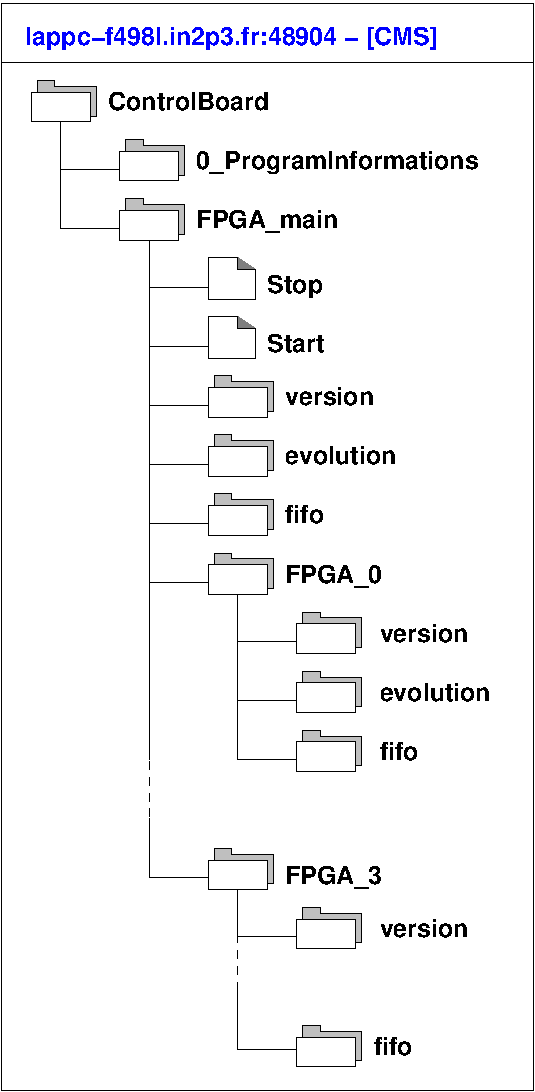
\includegraphics[width=5cm]{appendix/images/MOS_device_example_1.pdf}
\end{center}
\caption{Example of a  device managed through a MOS  server.  The root
  device is named \texttt{ControlBoard}.  First level daughter devices
  are  \texttt{0\_ProgramInformations} and  \texttt{FPGA\_main}.  Here
  the          MOS/OPCUA          server          is          labelled
  \texttt{CMS}.}\label{fig:an:mos_dev_1}
\end{figure}

% TODO


\subsection{Integration of a new device in the Vire environment}

The Vire  API also implements a  mechanism to describe a  hierarchy of
devices.  This  mechanism is independant  of the  one used in  the MOS
system but can  be easily made compatible with it.   This means that a
MOS  hierarchy  of devices  can  be  represented  in Vire.   The  Vire
hierarchy of  devices can  be considered as  some kind  of filesystem,
each device  being a folder with  its unique path, as  shown on figure
\ref{fig:an:mos_dev_2}.   The \emph{methods}  associated to  a devices
(or a datapoint) can be considered as plain executable files stored in
the  device's folder  : they  constitute the  set of  \emph{resources}
associated to the device.


\begin{figure}[h]
\begin{center}
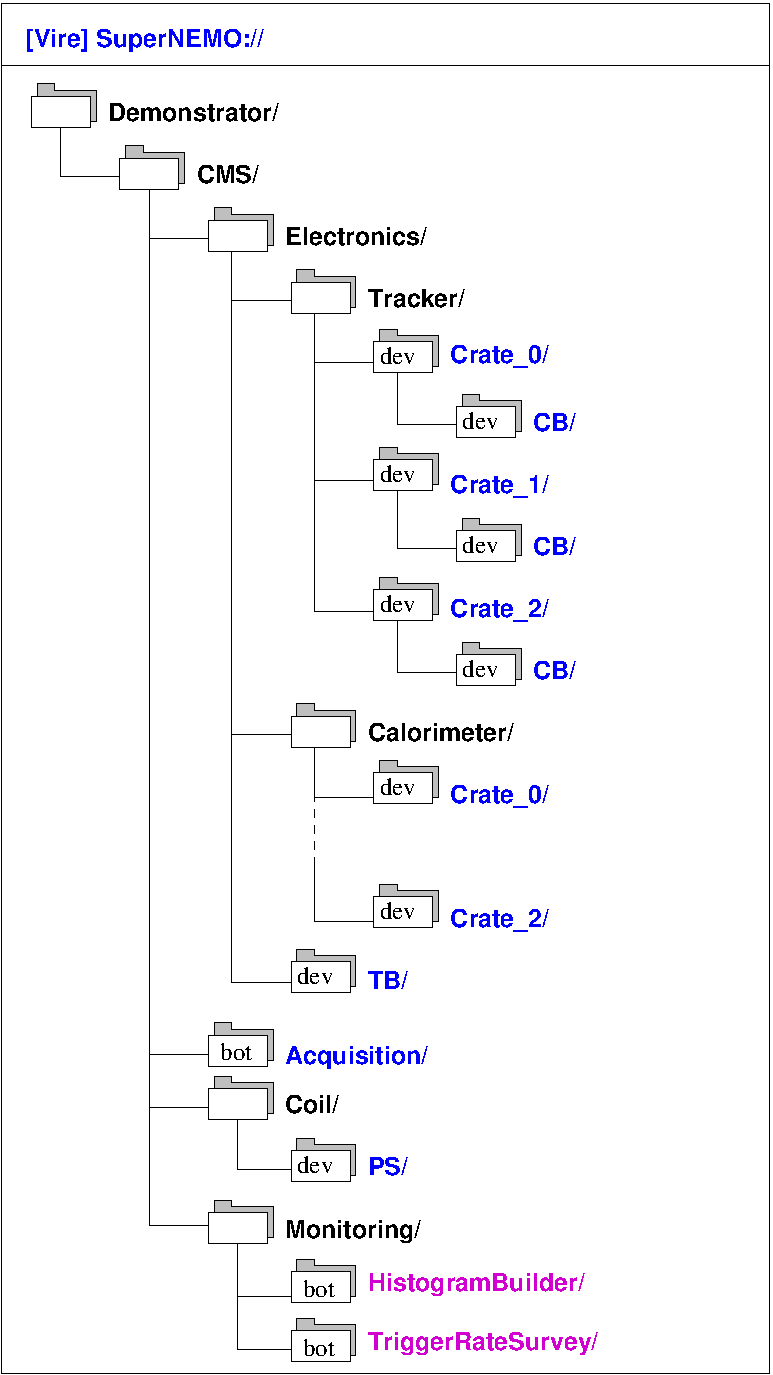
\includegraphics[width=5cm]{appendix/images/MOS_device_example_2.pdf}
\end{center}
\caption{Example of a hierarchy of  devices described by the Vire API.
  The root device is named  \texttt{SuperNEMO:}.  The top level (root)
  device  is  named  \texttt{Demonstrator}.  The  devices  colored  in
  \textcolor{blue}{blue}  are managed  through MOS/OPCUA.  The devices
  colored in \textcolor{magenta}{magenta} are directly embedded in the
  Vire server.  Devices with the \texttt{dev} tag are typical hardware
  device.  Devices  with the  \texttt{bot}  tag  are typical  software
  devices.   The  devices  colored in  \textbf{black}  are  structural
  pseudo-devices used to organize and  present a comprehensive view of
  the hierarchy. }\label{fig:an:mos_dev_2}
\end{figure}

The organisation of this hierarchy of devices is arbitrary and defined
by the designer of the  \emph{Control and Monitoring System}.  What is
important  to  understand  is  that  some  of  these  devices  can  be
associated  to  \emph{hardware  devices}  (a  power  supply  crate,  a
temperature probe\dots) and others  can be \emph{pseudo-devices}, i.e.
pure   software  object   (a   monitoring  robot,   a  file   transfer
daemon\dots).

In the context of the coupling of  the Vire server and the CMS server,
we are  in the event that  some devices are managed  by some MOS/OPCUA
servers and others are managed  in the Vire server itself.  Typically,
\emph{hardware devices}  are systematically managed through  the OPCUA
technology.  Vire has a mechanism to integrate such devices in its own
hierarchy.  This mechanism can  be considered like the \emph{mounting}
of   a   remote   filesystem   from  a   local   filesystem.    Figure
\ref{fig:an:mos_dev_0} illustrates  the case of many  hardware devices
-- managed by MOS -- that are integrated in the Vire system.  From the
Vire point of  view, the user does not see  the implementation details
for such  devices. He  does not  know the identity  of the  MOS server
hosting the device. He does not even know if the device is hosted by a
MOS server.  Devices are simply visible through the standard hierarchy
published by Vire with its  own device naming scheme, regardless their
true location.



\begin{figure}[h]
\begin{center}
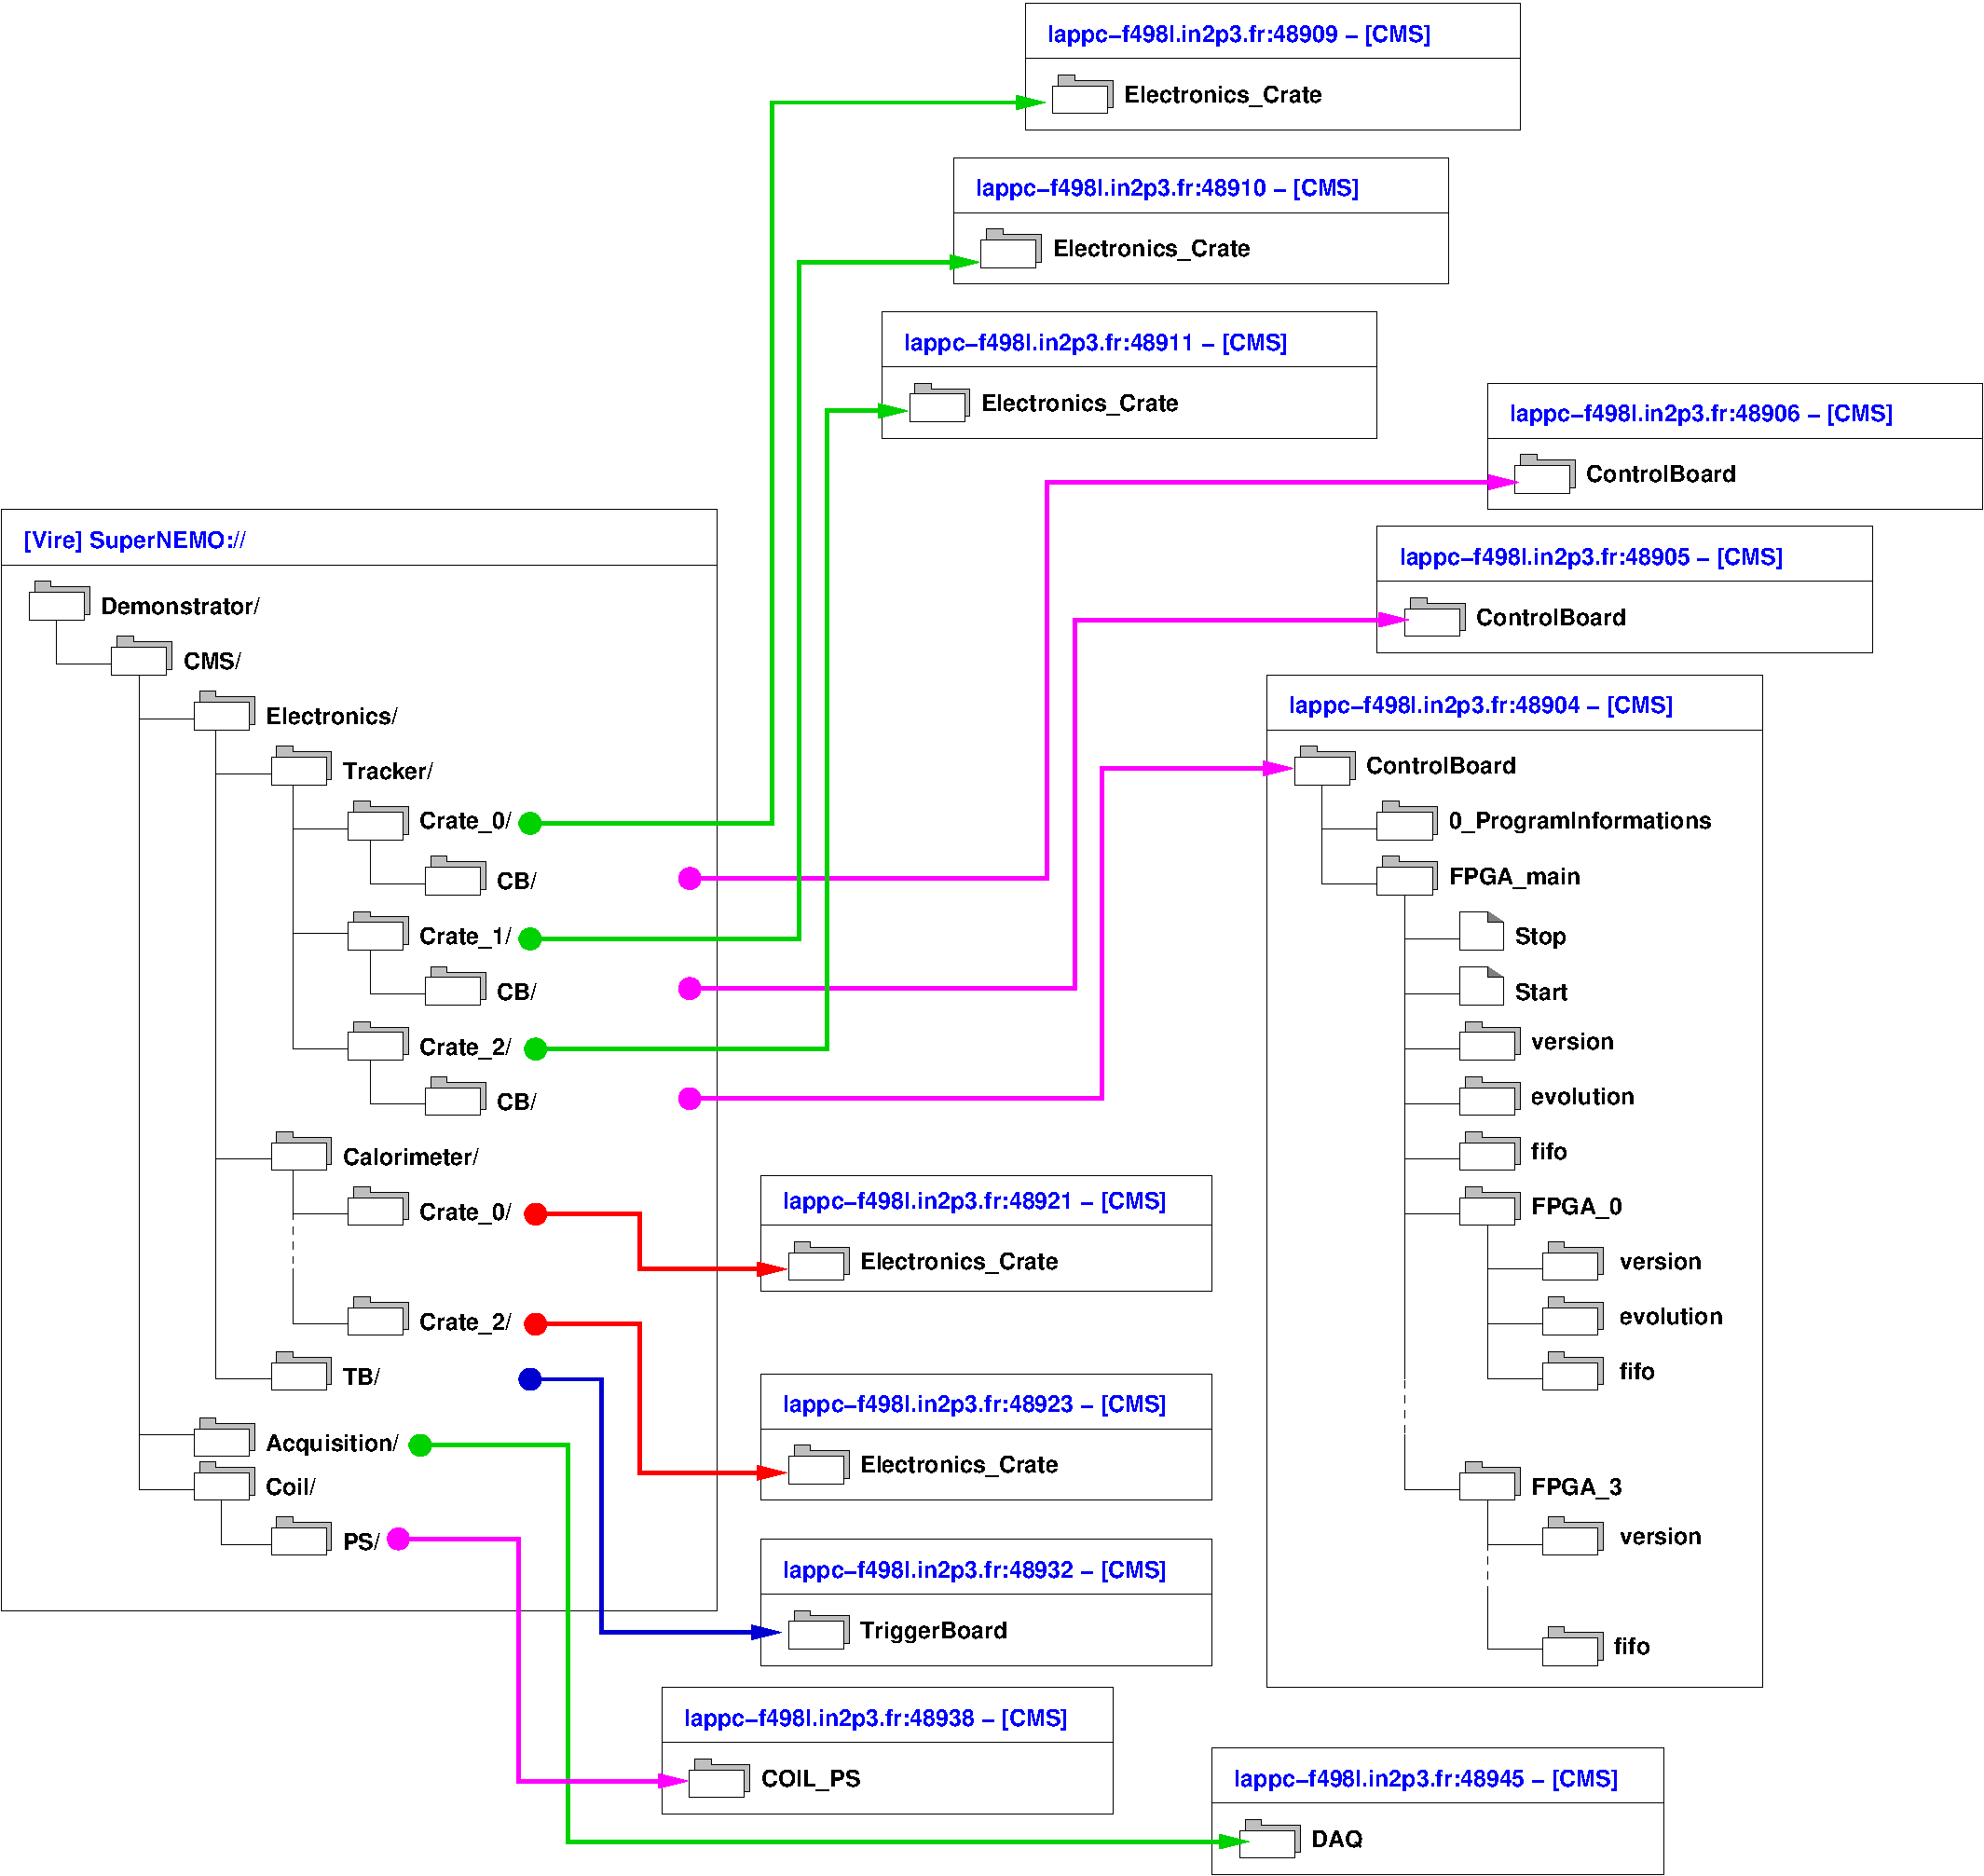
\includegraphics[width=\linewidth]{appendix/images/MOS_device_example_0.pdf}
\end{center}
\caption{The  mounting of  many  MOS device  hierarchies  in the  Vire
  device hierarchy.  Each OPCUA server  runs a simple  hardware device
  that is \emph{mounted} from a specific node with its own path.
%% of  devices described by the Vire API.
%%   The root device is named  \texttt{SuperNEMO:}.  The top level (root)
%%   device is  named \texttt{Demonstrator}. The devices  colored in blue
%%   are managed  through MOS/OPCUA. The  devices colored in  magenta are
%%   directly embedded in the Vire server.  Devices with the \texttt{dev}
%%   tag are typical  hardware device. Devices with  the \texttt{bot} tag
%%   are typical software devices.
}\label{fig:an:mos_dev_0}
\end{figure}




\subsection{Example}

Using  the examples  displayed  in  figure \ref{fig:an:mos_dev_0},  we
consider  in detail  the way  one specific  device managed  by MOS  is
mounted   in  the   Vire   hierarchy.  Figure   \ref{fig:an:mos_dev_3}
illustrates the mounting of a MOS device in Vire.

Here the Vire  server publishes the path of a  device representing the
control board  of the third  electronic crate  for the tracker  of the
SuperNEMO demonstrator module.  The full Vire path of this device is:

\textcolor{blue}{\texttt{SuperNEMO://Demonstrator/CMS/Electronics/Tracker/Crate\_2/CB}}

This is  the only Vire identifier  recognized by user to  address this
device.

On    the   figure,    one    can   see    that    the   MOS    server
\texttt{lappc−f498l.in2p3.fr} (port 48904) hosts a simple device which
is locally named \texttt{ControlBoard}.

When  mounting   this  device  in   the  Vire  hierarchy,   the  local
\texttt{[CMS]}  namespace and  \texttt{ControlBoard} device  names are
hidden and replaced by the Vire device path.  All daughter devices and
datapoints of  the \texttt{CMS/ControlBoard} device are  integrated as
daughters        of        the         Vire        device        named\\
\texttt{SuperNEMO://Demonstrator/CMS/Electronics/Tracker/Crate\_2/CB}.


For example, the \texttt{FPGA\_main} daughter device is now associated
to the following Vire path:

\textcolor{blue}{\texttt{SuperNEMO://Demonstrator/CMS/Electronics/Tracker/Crate\_2/CB/FPGA\_main/}}

and  its  \texttt{Stop} method  is  automatically  addressed with  the
following \emph{leaf} path:

\textcolor{blue}{\texttt{SuperNEMO://Demonstrator/CMS/Electronics/Tracker/Crate\_2/CB/FPGA\_main/Stop}}


\begin{figure}[h]
\begin{center}
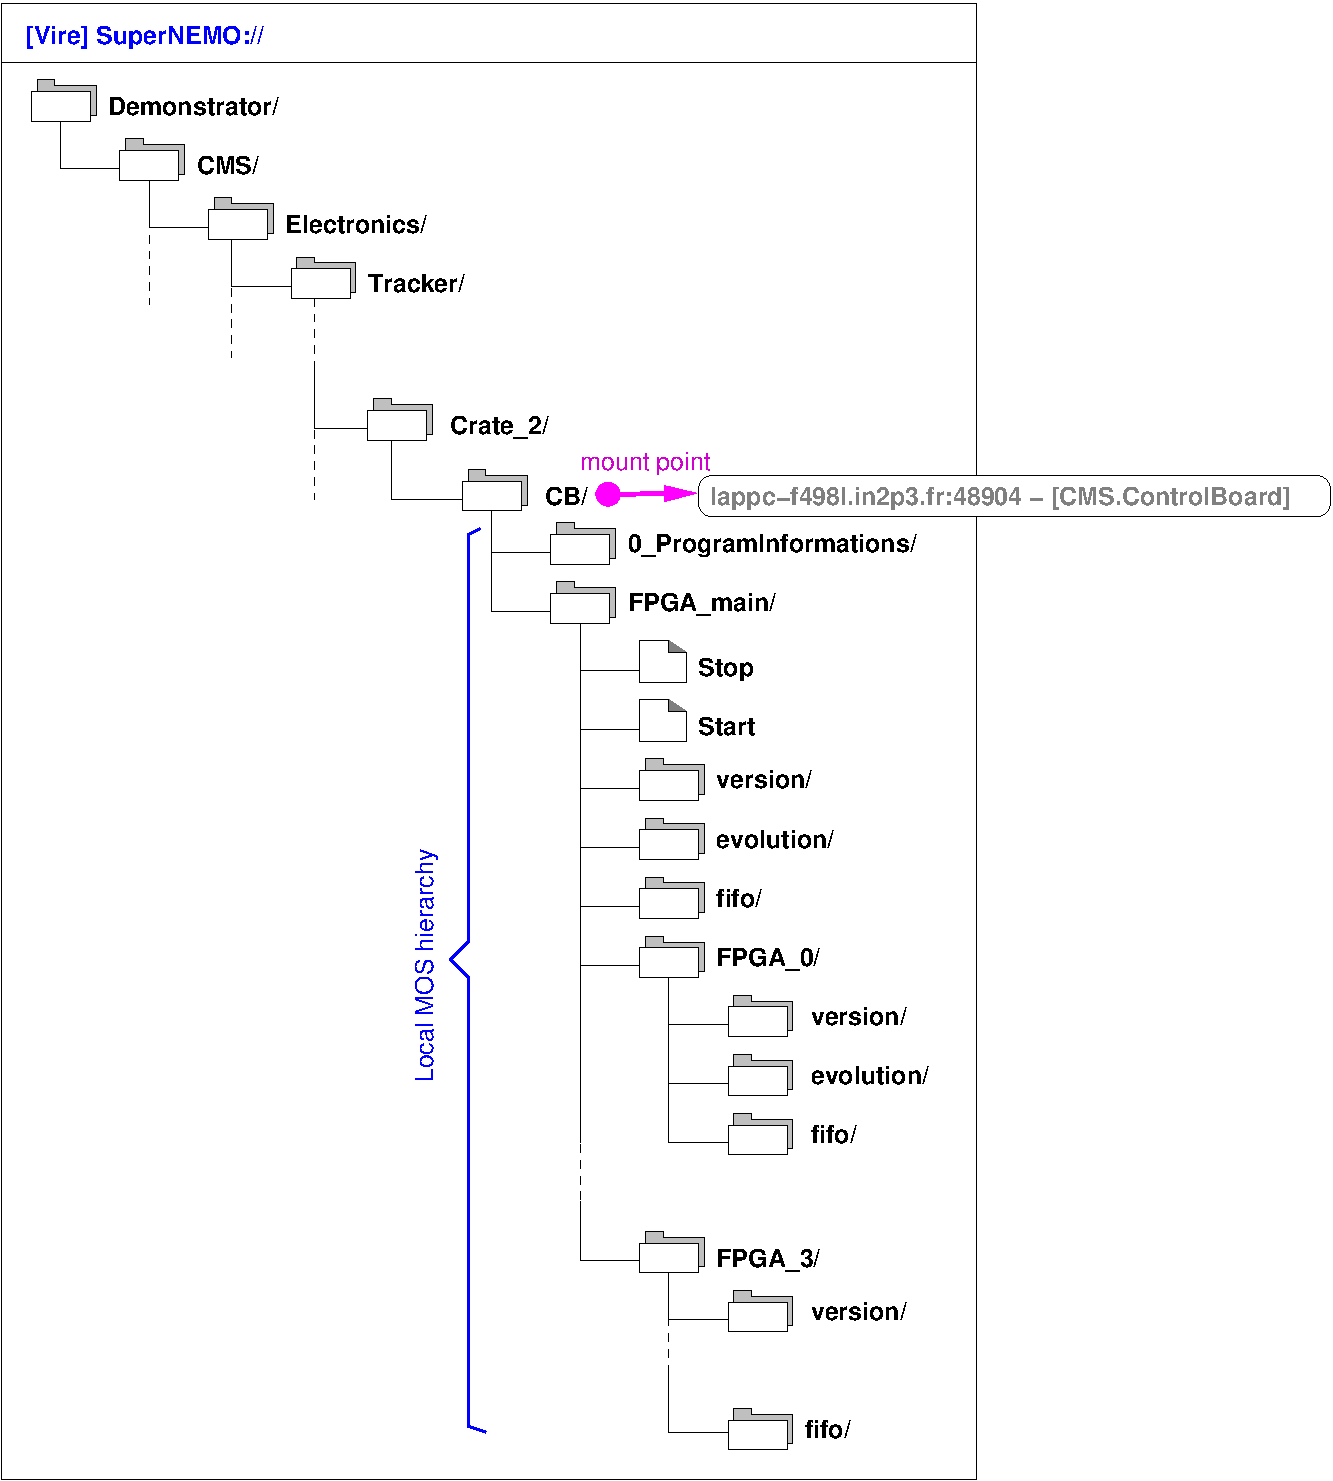
\includegraphics[width=0.8\linewidth]{appendix/images/MOS_device_example_3.pdf}
\end{center}
\caption{The  mounting of  one  MOS device and its local hierarchy  in the  Vire
  device hierarchy.}\label{fig:an:mos_dev_3}
\end{figure}



\subsection{Vire/MOS mapping}

As it can be  seen in the above example, the integration  of a new MOS
device in the Vire system is  achieved through soem kind of filesystem
mounting operation.   Particularly, it is  shown that the MOS  name of
the   mounted  root   device  is   replaced  by   an  arbitrary   Vire
path. However, all daughter  nodes (devices, datapoints) attached from
this root  node have their  relative MOS  names preserved in  the Vire
naming scheme.

Any  resource  (method)  associated  to any  of  such  daughter  nodes
inherits this relative naming scheme.

As Vire applications  describe resources through their  Vire paths, it
is thus needed to build an explicit map that associates resource paths
to MOS address  and name. The CMS  server will be able  to resolve the
MOS server/port and  embedded device associated to  the resource path.

The goal of the \texttt{devices\_launch.conf} file is not only to tell
the CMS server what MOS server should  be loaded and ran at start, but
also  to describe  the  \emph{mounting point/names}  used  by Vire  to
access the resources associated to MOS devices.  From the informations
stored in the  file, an explicit associative array must  be built when
the Vire server connect to the CMS server.  It will play the role of a
resource path resolver  when requests about resources will  be sent by
Vire applications.  This associative array  must be locked  during the
Vire/CMS connection.



%\subsubsection{Preparation of XML device models}

%% \noindent\underline{Pre-condition:}
%% The device is working and validated through the MOS/OPCUA server

%% \begin{enumerate}

%% \item Produce XML décrivant le modèle du device enrichi
%%   des metadata
%% Rédaction du fichier XML décrivant le modèle du device

%% \item Génération des fichiers model du type de device pour Vire

%% \item Génération des fichiers instances resolv.conf

%% \end{enumerate}


\vfill
\pagebreak
\clearpage

% end


\section{Vire messages}\label{app:vire_messages}

Within Vire  and between Vire  components and external  components, we
use  a communication  system  based on  Vire  messages.  This  section
describes the structure of such messages.

\subsection{General structure of a message}

Each message consists in two parts (figure \ref{fig-vire-message-message-cpp}):
\begin{itemize}

\item  the  \emph{header}  is   dedicated  to  generic  and  typicalle
  mandatory  informations  which  document   the  message  itself  and
  arbitrary high-level metadata.

\item  the \emph{body}  of the  message  contains the  real data: the payload.
  The structure of the message body depends on some convention. Vire uses
  its own convention to embed the payload data.

\end{itemize}

\begin{figure}[h]
\vskip 10pt
\small
\begin{Verbatim}[frame=single,xleftmargin=0.cm,label=\fbox{C++}]
struct vire::message::message {
  message_header header; // Header of the message
  message_body   body;   // Body of the message
};
\end{Verbatim}
\normalsize
\caption{The structure of a Vire message object (C++  class:
  \texttt{"vire::message::message"})}\label{fig-vire-message-message-cpp}
\end{figure}

\subsection{The message header}

The header contains (figure \ref{fig-vire-message-message_header-cpp}):
\begin{itemize}

  \item The mandatory \texttt{message\_id}  attribute is an identifier
    of the  message which  document the emitter  and a  unique message
    number.   Each emitter  is  responsible of  the  numbering of  the
    messages it  emits, typically using an  incremental technique. The
    message  number is  a positive  integer, starting  from 0  (figure
    \ref{fig-vire-message-message_identifier-cpp}).

  \item  The \texttt{timestamp}  attribute  encodes the  approximative
    time point when the message was  created. It contains the date and
    the time, using at least microsecond resolution.

    Typically,  with  JSON  encoding  system, it  is  expected  to  be
    formatted as a character string, using the following ISO format:

    \begin{center}
      \texttt{yyyymmddThhmmss.uuuuuu}
    \end{center}

    \noindent where:

    \vskip -10pt
    \begin{itemize}
    \item[\texttt{yyyymmdd} :] encodes year/month/day,
    \item[\texttt{hhmmssd} :] encodes hour/minute/second,
    \item[\texttt{uuuuuu} :] encodes microseconds.
    \end{itemize}

  \item   In   the   case    of   a   \emph{response}   message,   the
    \texttt{in\_reply\_to} attribute is set to identify the associated
    request message.

  \item  The \texttt{asynchronous}  boolean  attribute is  set if  the
    message processing  is explicitely requested  by the source  to be
    asynchronous (non-blocking).  In  RPC transactions, where requests
    are transmitted from one point to  the other, its default value is
    \emph{false}.   It  is possible  to  force  a RPC  transaction  in
    asynchronous mode.   This use  case is documented  elsewhere.  For
    event messaging, this flag is conventionally set to \emph{true}.

  \item  The  \texttt{body\_layout\_id}  attribute  is  the  mandatory
    identifier   of   the   layout   of  the   message   body   (class
    \texttt{"vire::utility::model\_identifier"}).  The  default layout
    for     message     body     inside    the     Vire     API     is
    \texttt{"vire::message::body\_format::typed\_payload"}, with version
    \texttt{"1.0"}                                             (figure
    \ref{fig-vire-utility-model_identifier-cpp}).

\end{itemize}


\begin{figure}[h]
\vskip 10pt
\small
\begin{Verbatim}[frame=single,xleftmargin=0.cm,label=\fbox{C++}]
struct vire::message::message_header {
  message_identifier message_id;     // Message identifier from the emitter.
  std::string        timestamp;      // Timestamp.
  message_identifier in_reply_to;    // Message identifier of the associated
                                     // request message (optional).
  bool               asynchronous,   // Asynchronous flag.
  vire::utility::model_identifier     body_layout_id; // Body layout identifier.
  std::map<std::string, std::string>  metadata;       // Key/value metadata dictionary.
};
\end{Verbatim}
\normalsize
\caption{The  structure  of  a   message  header  object  (C++  class:
  \texttt{"vire::message::message\_header"}).}\label{fig-vire-message-message_header-cpp}
\end{figure}

\begin{figure}[h]
\vskip 10pt
\small
\begin{Verbatim}[frame=single,xleftmargin=0.cm,label=\fbox{C++}]
struct vire::message::message_identifier {
  std::string emitter; // Name identifying the emitter of the message.
  int32_t     number;  // Number identifying the message in the emitter's
                       // message numbering scheme.
};
\end{Verbatim}
\normalsize
\caption{The      structure      of     a      message      identifier
  (C++  class:  \texttt{"vire::message::message\_identifier"}).}
\label{fig-vire-message-message_identifier-cpp}
\end{figure}

\begin{figure}[h]
\vskip 10pt
\small
\begin{Verbatim}[frame=single,xleftmargin=0.cm,label=\fbox{C++}]
struct vire::utility::model_identifier {
  std::string name;    // Name identifying the format of the message.
  std::string version; // String identifying the version of the format.
};
\end{Verbatim}
\normalsize
\caption{The structure of a model identifier (C++  class:  \texttt{"vire::utility::model\_identifier"}.}\label{fig-vire-utility-model_identifier-cpp}
\end{figure}




\begin{figure}[h]
\vskip 10pt
\small
\begin{Verbatim}[frame=single,xleftmargin=0.cm,label=\fbox{JSON}]
{
   "header" : {
      "message_id" : {
         "emitter" : "vire.server",
         "number" : 42
      },
      "timestamp" : "20160930T141408.413443",
      "in_reply_to" : {
         "initialized" : true,
         "value" : {
            "emitter" : "vire.client.0",
            "number" : 23
         }
      },
      "asynchronous" : false,
      "body_layout_id" : {
         "name" : "vire::message::body_format::typed_payload",
         "version" : {
            "initialized" : true,
            "value" : "1.0"
         }
      },
      "metadata" : [
         {
            "key" : "key1",
            "value" : "foo"
         },
         {
            "key" : "key2",
            "value" : "42"
         },
         {
            "key" : "key3",
            "value" : "3.1415899999999999"
         },
         {
            "key" : "key4",
            "value" : "true"
         }
      ]
   }
  "body" : {
      ...
   }
}
\end{Verbatim}
\normalsize
\caption{Example of  a   message  header  object in JSON format.}
\label{fig-vire-message-message_header-json}
\end{figure}

\vfill
\clearpage
\pagebreak

\subsection{The message body}

The    default    message   body    layout    in    Vire   is    named
\texttt{"vire::message::body\_format::typed\_payload"}        (version
\texttt{"1.0"}).   Each  message used  within  the  Vire framework  is
supposed to use this layout.  The general idea is that the body of the
message embeded the  \emph{payload object} that has  to be transmitted
between  two components  of  the system.   \emph{Payload objects}  are
classified in one of the three following categories:

\begin{enumerate}

\item \emph{Request}:  describes a request submitted  by one component
  to another component (generally during a synchronous RPC transaction).

\item  \emph{Response}: describes  the  response to  a former  request
  (generally during a synchronous RPC transaction).

\item \emph{Event}: describes an  arbitrary information record (alarm,
  exception, signal\dots) which is transmitted asynchronously.

\end{enumerate}

Vire implements the following class hierarchy:

\begin{center}
\begin{tikzpicture}
  \node (payload)  at (0,2)  [draw] {\texttt{vire::utility::base\_payload}};
  \node (request)  at (-4,0) [draw] {\texttt{vire::utility::base\_request}};
  \node (response) at (2,0)  [draw] {\texttt{vire::utility::base\_response}};
  \node (event)    at (8,0)  [draw] {\texttt{vire::utility::base\_event}};

  %\draw[style=help lines] (-3,-1) grid (10,4);
  \draw (node cs:name=response,anchor=north) |- (0,1);
  \draw (node cs:name=event,anchor=north)    |- (0,1);
  \draw[->] (node cs:name=request,anchor=north)
  |- (0,1) -| (node cs:name=payload,anchor=south);
\end{tikzpicture}
\end{center}

The requirements for the transmitted object are the following:

\begin{itemize}

\item The  type of the object  must be conventionally associated  to a
  unique     \emph{model      identifier}     object      (see     the
  \texttt{"vire::utility::model\_identifier"} class)  which contains a
  unique   name   (\textit{string    identifier})   and   possibly   a
  \textit{version identifier}.  Each software  component that may send
  or  receive the  object  should agree  on  this type  identification
  scheme.   This   enable  the  use  of   object  factories,  whatever
  programming  langage  is used  on  both  side of  the  communication
  system.

\item  For each  software component,  the object  type must  have some
  dedicated  encoding/decoding  functions  available  (again  whatever
  programming language is used). For example the Vire API supports the
  following encoding formats:

  \begin{itemize}

  \item JSON (MIME  encoding type: \texttt{"application/x-json"}), which
    is supportable by many languages,

  \item  Protobuf  (Google  Protocol   Buffers,  MIME  encoding  type:
    \texttt{"application/x-protobuf"}), which is also widely supported,

  \item   Boost/serialisation   (XML,    text   or   binary   archives
    \texttt{"application/x-boost-serialization-xml"},
    \texttt{"application/x-boost-serialization-text"},
    \texttt{"application/x-boost-serialization-binary"}),    which    in
    principle is supported by C++ only.

  \end{itemize}

  The Protobuf  encoding format will be  used to serialize/deserialize
  the  Vire  messages transported  between  the  Vire server  and  the
  CMS/LAPP server.

\end{itemize}

Vire uses a dedicated layout to represent the body of any message with
its embedded payload object. With this technique, the structure of the
body          contains         two          attributes         (figure
\ref{fig-app-vire-message-message_body-cpp}):

\begin{enumerate}

\item The \texttt{payload\_type\_id} specifies the type of the payload
  object   (figure   \ref{fig-app-vire-utility-model_identifier-cpp}).
  This unique name  is conventionaly fixed for a  given application. A
  version tag allows to support possible evolution of the object type.

\item The  \texttt{payload} is a  handle to  a payload object  of type
  request, response or event.

  %% \begin{itemize}
  %% \item Within  the producer  component of  the message,  the encoding
  %%   function associated to the object  type is responsible to generate
  %%   the JSON stream for the object and store it in the buffer.

  %% \item Within  the consumer  component of  the message,  the decoding
  %%   function associated to the object type is responsible to parse the
  %%   JSON stream stored in the buffer and restore the object in memory.

  %% \end{itemize}

  It is expected  that, on both sides of the  connection, the software
  components can  access dedicated  software plugins which  ensure the
  support  of  various   \emph{payload  object  types}  conventionnaly
  associated  with  their  \emph{payload type  identifiers}  and  also
  providing JSON and/or Protobuf encoding/decoding functionalities.

  %% The   system  allows  to  support
  %% modification  in the  structure of  the objects  thanks to  version
  %% tagging.

\end{enumerate}

\begin{figure}[h]
\vskip 10pt
\small
\begin{Verbatim}[frame=single,xleftmargin=0.cm,label=\fbox{C++}]
struct message_body {
  vire::utility::model_identifier     payload_type_id; // Object type identifier.
  const vire::utility::base_payload * payload;         // Handle to a payload object.
};
\end{Verbatim}
\normalsize
\caption{The structure of a message body object (C++).}
\label{fig-app-vire-message-message_body-cpp}
\end{figure}

\begin{figure}[h]
\vskip 10pt
\small
\begin{Verbatim}[frame=single,xleftmargin=0.cm,label=\fbox{JSON}]
{
  "header" : {
    ...
  },
  "body" : {
    "payload_type_id" : {
      "name" : "vire::message::testing::error_event",
      "version" : {
        "initialized" : false
      }
    },
    "payload" : {
      "timestamp" : "20160930T141743.759085"
      "err" : {
        "code" : 3,
        "message" : "A basic error"
      },
    }
  }
}
\end{Verbatim}
\normalsize
\caption{Example of  a   message  body  object in JSON format.}
\label{fig-vire-message-message_body-json}
\end{figure}

\vfill
\clearpage
\pagebreak

% end

%\input{appendix/app_json_fmt.tex}

\section{The \emph{Protocol Buffers} format}\label{app:protobuf_fmt}

\subsection{Introduction}

The  Google  Protocol Buffers  (\emph{protobuf})  library  is used  to
represent the objects that are exchanged between the Vire clients, the
Vire server and the CMS server.  The  version 3 of the format is used,
implying   at   least   version   3.0.0  (September   2016)   of   the
\emph{protobuf} library.

Each  data   structure  of  interest   can  be  described   through  a
\texttt{.proto}  file  from  which  stub files  can  be  automatically
generated  with the  \texttt{protoc} compiler.  For Vire  and its  CMS
interface, the C++ and Java programming languages will be used.


A  collection of  \texttt{.proto}  files are  provided  with the  Vire
library to represent all kind  of data structures transferable between
networked agents  (Vire server,  Vire clients, CMS/LAPP  server).  The
objects of  the highest level  are named \emph{payload  objects} (like
\emph{request},  \emph{response} and  \emph{event} objects).   They
are composed of attributes of more basic data structures.

\subsection{Example}

The following  class diagram  illustrates two data  structures defined
within the Vire library with an inheritance relationship between them.

\begin{center}
  \begin{tikzpicture}
    \node (base)     at (0,1.5)  [draw] {\texttt{vire::utility::base\_error}};
    \node (setup)    at (0,0)  [draw] {\texttt{vire::utility::invalid\_setup\_id\_error}};

    \draw[->]   (node cs:name=setup,anchor=north) |- (0,1);
    |- (0,1) -| (node cs:name=base,anchor=south);
  \end{tikzpicture}
\end{center}

The \texttt{vire::utility::base\_error}  is the  parent class  for all
\emph{error}  objects.   It  contains   two  attributes:   an  integer
\emph{error code}  and a  character string describing  the \emph{error
  message}.

The   \texttt{vire::utility::invalid\_setup\_id\_error}  class   is  a
specialized error class  which represents explicitely an  error due to
an identification  failure of  the experimental setup.   It implements
additional mutually exclusive attributes: the \emph{unrecognized name}
of the setup or the \emph{unrecognized version} of the setup.

This   example  illustrates   the  protobuf   representation  of   the
\texttt{vire::utility::base\_error}  in the  Vire  library, using  the
\texttt{"vire/utility/BaseError.proto"} file:

\small
\begin{Verbatim}[frame=single,xleftmargin=0.cm,label=\fbox{protobuf}]
  syntax = "proto3";
  package vire.utility; // Namespace

  message BaseError {

    // reserved 1; // Reserved for _base message

    // Attributes:
    int32  code           = 100; // The error code
    string message_format = 101; // The error description message

  }
\end{Verbatim}
\normalsize

\vfill
\clearpage
\pagebreak

\subsection{Vire protobuf conventions}

Vire uses the following conventions:

\begin{enumerate}

\item
  The member index  \texttt{1} is reserved to represent the  link of a
  class to its main base/parent class (if any).  It is not used if the
  data structure does not inherit any data structure.
  If a data structure naturally inherits another one, it is thus possible
  to  represent the  inheritance  relationship as  illustrated with  the
  \texttt{"vire/utility/InvalidSetupIdError.proto"}      file      which
  represents the \texttt{vire::utility::invalid\_setup\_id\_error} class
  in the Vire library:

  \small
  \begin{Verbatim}[frame=single,xleftmargin=0.cm,label=\fbox{protobuf}]
    syntax = "proto3";
    package vire.utility; // Namespace

    import "vire/utility/BaseError.proto"; // Dependency

    message InvalidSetupIdError {

      BaseError _base = 1; // The base class

      // Additional attributes:
      oneof detail { // Mutual exclusion
        string invalid_setup_name    = 100; // The failed setup name
        string invalid_setup_version = 101; // The failed setup version
      }

    }
  \end{Verbatim}
  \normalsize

\item The  \texttt{\_base} member  is conventionally  used to  represent the
  inheritance   relationship    from   a   data   structure    of   type
  \texttt{"vire.utility.BaseError"}.

\item Member indexes from \texttt{2}  to \texttt{99} are also reserved
  for possible future usage (multiple inheritance, metadata\dots).

\item
  The first member of the data structure must start at index \texttt{100}.

\end{enumerate}

\vfill
\clearpage
\pagebreak

% end


\section{Vire payload objects}\label{app:payload}

\subsection{Introduction}

As  mentioned in  appendix \ref{app:protobuf_fmt},  Vire messages  are
wrappers for \emph{payload objects}.  Each  type of payload object can
be represented  through the \emph{protobuf} mechanism.   The following
class hierarchy shows the base architecture used to define new payload
objects.

\begin{center}
\begin{tikzpicture}
  \node (payload)  at (0,2)   [draw] {\texttt{vire::utility::base\_payload}};
  \node (request)  at (-4,0)  [draw] {\texttt{vire::utility::base\_request}};
  \node (response) at (2,0)   [draw] {\texttt{vire::utility::base\_response}};
  \node (event)    at (8,0)   [draw] {\texttt{vire::utility::base\_event}};
  \node (my)       at (-4,-2) [draw] {\texttt{my\_request}};
  \node (your)     at (2,-2)  [draw] {\texttt{your\_response}};
  \node (its)    at (8,-2)    [draw] {\texttt{its\_alarm}};

  %\draw[style=help lines] (-6,-2) grid (10,2);
  \draw (node cs:name=response,anchor=north) |- (0,1);
  \draw (node cs:name=event,anchor=north)    |- (0,1);
  \draw[->] (node cs:name=request,anchor=north)
  |- (0,1) -| (node cs:name=payload,anchor=south);
  \draw[->] (node cs:name=my,anchor=north)
  |- (-4,-1) -| (node cs:name=request,anchor=south);
  \draw[->] (node cs:name=your,anchor=north)
  |- (2,-1) -| (node cs:name=response,anchor=south);
  \draw[->] (node cs:name=its,anchor=north)
  |- (8,-1) -| (node cs:name=event,anchor=south);
\end{tikzpicture}
\end{center}


\begin{center}
\vskip 10pt
\small
\begin{tabular}{|l|l|l|}
  \hline
  \textbf{Vire C++ class} & \textbf{protobuf message type} & \textbf{protobuf definition file} \\
  \hline
  \hline
  \multicolumn{3}{|c|}{\emph{general types}} \\
  \hline
  boost::posix\_time::ptime & google.protobuf.Timestamp & google/protobuf/timestamp.proto \\
  \hline
  \hline
  \multicolumn{3}{|c|}{\emph{identifier types}} \\
  \hline
  vire::utility::base\_identifier & vire.utility.Baseidentifier & vire/utility/Baseidentifier.proto \\
  \hline
  vire::utility::instance\_identifier & vire.utility.InstanceIdentifier & vire/utility/InstanceIdentifier.proto \\
  \hline
  vire::utility::model\_identifier & vire.utility.ModelIdentifier & vire/utility/ModelIdentifier.proto \\
  \hline
  \hline
  \multicolumn{3}{|c|}{\emph{error types}} \\
  \hline
  vire::utility::base\_error & vire.utility.BaseError & vire/utility/BaseError.proto \\
  \hline
  vire::utility::invalid\_context\_error & vire.utility.InvalidContextError & vire/utility/InvalidContextError.proto \\
  \hline
  vire::utility::invalid\_setup\_id\_error & vire.utility.InvalidSetupIdError & vire/utility/InvalidSetupIdError.proto \\
  \hline
  \hline
  \multicolumn{3}{|c|}{\emph{payload types}} \\
  \hline
  vire::utility::base\_payload & vire.utility.BasePayload & vire/utility/BasePayload.proto \\
  \hline
  vire::utility::base\_request & vire.utility.BaseRequest & vire/utility/BaseRequest.proto \\
  \hline
  vire::utility::base\_response & vire.utility.BaseResponse & vire/utility/BaseResponse.proto \\
  \hline
  vire::utility::base\_event & vire.utility.BaseEvent & vire/utility/BaseEvent.proto \\
  \hline
  vire::utility::base\_alarm & vire.utility.BaseAlarm & vire/utility/BaseAlarm.proto \\
  \hline
  \hline
  \multicolumn{3}{|c|}{\emph{messenging types}} \\
  \hline
  vire::message::message\_identifier & vire.message.MessageIdentifier & vire/message/MessageIdentifier.proto \\
  \hline
  vire::message::msg\_header & vire.message.MsgHeader & vire/message/MsgHeader.proto \\
  \hline
  vire::message::msg\_body & vire.message.MsgBody & vire/message/MsgBody.proto \\
  \hline
  vire::message::message & vire.message.Message & vire/message/Message.proto \\
  \hline
\end{tabular}
\normalsize
\end{center}


\begin{center}
\vskip 10pt
\small
\begin{tabular}{|l|l|l|}
  \hline
  \multicolumn{3}{|c|}{\emph{Resource management related types}} \\
  \hline
  vire::cms::resource\_status\_record & vire.cms.ResourceStatusRecord & vire/cms/ResourceStatusRecord.proto \\
  \hline
  vire::cms::resource\_fetch\_status\_request & vire.cms.ResourceFetchStatusRequest & vire/cms/ResourceFetchStatusRequest.proto \\
  \hline
  vire::cms::resource\_fetch\_status\_success\_response & vire.cms.ResourceFetchStatusSuccessResponse & vire/cms/ResourceFetchStatusSuccessResponse.proto \\
  \hline
  vire::cms::resource\_fetch\_status\_failure\_response & vire.cms.ResourceFetchStatusFailureResponse & vire/cms/ResourceFetchStatusFailureResponse.proto \\
  \hline
  vire::cms::resource\_exec\_request & vire.cms.ResourceExecRequest & vire/cms/ResourceExecRequest.proto \\
  \hline
  vire::cms::resource\_exec\_success\_response & vire.cms.ResourceExecSuccessResponse & vire/cms/ResourceExecSuccessResponse.proto \\
  \hline
  vire::cms::resource\_exec\_failure\_response & vire.cms.ResourceExecFailureResponse & vire/cms/ResourceExecFailureResponse.proto \\
  \hline
  vire::cms::resource\_exec\_non\_blocking\_request & vire.cms.ResourceExecNonBlockingRequest & vire/cms/ResourceExecNonBlockingRequest.proto \\
  \hline
  vire::cms::resource\_exec\_non\_blocking\_ack\_response & vire.cms.ResourceExecNonBlockingAckResponse & vire/cms/ResourceExecNonBlockingAckResponse.proto \\
  \hline
  vire::cms::resource\_exec\_non\_blocking\_noack\_response & vire.cms.ResourceExecNonBlockingNoackResponse & vire/cms/ResourceExecNonBlockingNoackResponse.proto \\
  \hline
  vire::cms::resource\_exec\_non\_blocking\_success\_event & vire.cms.ResourceExecNonBlockingSuccessEvent & vire/cms/ResourceExecNonBlockingSuccessEvent.proto \\
  \hline
  vire::cms::resource\_exec\_non\_blocking\_failure\_event & vire.cms.ResourceExecNonBlockingFailureEvent & vire/cms/ResourceExecNonBlockingFailureEvent.proto \\
  \hline
  vire::cms::resource\_exec\_error & vire.cms.ResourceExecError & vire/cms/ResourceExecError.proto \\
  \hline
  vire::cms::invalid\_status\_error & vire.cms.ResourceExecError & vire/cms/ResourceExecError.proto \\
  \hline
  %% vire::cms::invalid\_credentials\_error & vire.cms.InvalidCredentialsError & vire/cms/InvalidCredentialsError.proto \\
  %% \hline
  %% vire::cms::invalid\_user\_error & vire.cms.InvalidUserError & vire/cms/InvalidUserError.proto \\
  %% \hline
  vire::cms::invalid\_resource\_error & vire.cms.InvalidUserError & vire/cms/InvalidUserError.proto \\
  \hline
  vire::cms::no\_pubsub\_resource\_error & vire.cms.NoPubsubResourceError & vire/cms/NoPubsubResourceError.proto \\
  \hline
  \hline
  \multicolumn{3}{|c|}{\emph{Resource pub/sub management types}} \\
  \hline
  vire::cms::resource\_pubsub\_subscribe\_request & vire.cms.ResourcePubsubSubscribeRequest & vire/cms/ResourcePubsubSubscribeRequest.proto \\
  \hline
  vire::cms::resource\_pubsub\_subscribe\_success\_response & vire.cms.ResourcePubsubSubscribeRSuccessResponse & vire/cms/ResourcePubsubSubscribeRSuccessResponse.proto \\
  \hline
  vire::cms::resource\_pubsub\_subscribe\_failure\_response & vire.cms.ResourcePubsubSubscribeRFailureResponse & vire/cms/ResourcePubsubSubscribeRSuccessResponse.proto \\
  \hline
  \hline
  \multicolumn{3}{|c|}{\emph{Vire/CMS server interface types}} \\
  \hline
  vire::cmsinterface::connection\_request & vire.cmsinterface.ConnectionRequest & vire/cmsinterface/ConnectionRequest.proto \\
  \hline
  vire::cmsinterface::connection\_success\_response & vire.cmsinterface.ConnectionSuccessResponse & vire/cmsinterface/ConnectionSuccessResponse.proto \\
  \hline
  vire::cmsinterface::connection\_failure\_response & vire.cmsinterface.ConnectionFailureResponse & vire/cmsinterface/ConnectionFailureResponse.proto \\
  \emph{embedded:} unknown\_resources\_error & .UnknownResourcesError &  \\
  \hline
  vire::cmsinterface::disconnection\_request & vire.cmsinterface.DisconnectionRequest & vire/cmsinterface/DisconnectionRequest.proto \\
  \hline
  vire::cmsinterface::disconnection\_success\_response & vire.cmsinterface.DisconnectionSuccessResponse & vire/cmsinterface/DisconnectionSuccessResponse.proto \\
  \hline
  %% \hline
  %% vire::cmsinterface::disconnection\_failure\_response & vire.cmsinterface.DisconnectionFailureResponse & vire/cmsinterface/DisconnectionFailureResponse.proto \\
\end{tabular}
\normalsize
\end{center}

\subsection{Basic data structures}

Any  payload object  (request, response  or event)  generally contains
some information records which are  specific to the functionalities of
the  payload  object they  belong.   These  records are  of  arbitrary
types. Of course they should be  translatable in terms of the protobuf
library.
%Of course they can be (de)serialized using JSON.
Some of these types are very  general and defined within the Vire core
API itself because they are reused by various payload objects not only
through  the Vire-CMS/LAPP  interface  but also  between  Vire clients  and
servers, independently  of the  CMS/LAPP server.  However,  the use  of the
Protocol Buffers interface makes possible  to publish the interface of
such data to the outside world, including the CMS/LAPP server in priority.

%% Other one are specific to the Vire/CMS interface and thus managed only
%% in the \texttt{Vire\_CMSInterface} API.
These  types  are considered  as  \emph{basic}.  Among them  we  find:
generic error  types, generic  identifier types,  timestamps, resource
status records\dots We propose to describe them in this section.

Once a sufficient collection of  basic data record types is available,
it  is possible  to describe  high  level payload  object types  which
aggregate attributes of such types.

Other record  types are specific to  some payload objects and  will be
never  used outside  the scope  of these  payload objects.   Such data
structures will be  explicitely declared with the  payload object they
belong to, likely as embedded types/classes.


\subsubsection{Errors}

Some  \emph{response} or  \emph{event} payload  objects may  contain a
specific  error  record  object.   A  \emph{failure  response}  or  an
\emph{exception  event}  object will  generally  embed  such an  error
record object.

Each  \emph{error record}  is represented  by an  instance of  a given
error type.   Each of  the error  types defined  in Vire  inherits the
\texttt{vire::utility::base\_error}      base       class      (figure
\ref{fig-app-payload-base_error})   which   contains   the   following
attributes:

\begin{itemize}

\item the error code: A non zero  integer which is set to 1 by default
  (indicating  a  generic  failure  case).   The  error  code  can  be
  conventionally  set to  any positive  integer value  to represent  a
  specific error case, depending on the context.

\item the error  message: an optional human  readable character string
  which documents the error as usefully as possible.

\end{itemize}

\begin{figure}[h]
\vskip 10pt
\small
\begin{Verbatim}[frame=single,xleftmargin=0.cm,label=\fbox{C++}]
struct vire::utility::base_error
{
  // Attributes:
  int         code;           // Error code (>0).
  std::string message_format; // Error message (optional).
};
\end{Verbatim}
\normalsize
\caption{The structure of a \texttt{"vire::utility::base\_error"} object
  (C++).}
\label{fig-app-payload-base_error}
\end{figure}


%% An example of JSON formatted basic error object is given in figure
%% \ref{fig-app-payload-base_error-1}.
%%
%% \begin{figure}[h]
%% \vskip 10pt
%% \small
%% \begin{Verbatim}[frame=single,xleftmargin=0.cm,label=\fbox{\texttt{JSON}}]
%% {
%%   "code" : "42",
%%   "message_format" : "Invalid AMQP server port=[2341]"
%% }
%% \end{Verbatim}
%% \normalsize
%% \caption{JSON  formatted  basic  error  object  (class
%%   \texttt{vire::utility::base\_error}.}
%% \label{fig-app-payload-base_error-1}
%% \end{figure}

Several type of generic errors are defined in Vire:


\begin{center}
\begin{tikzpicture}
  \node (base)     at (0,2)  [draw] {\texttt{vire::utility::base\_error}};
  \node (context)  at (-4,0) [draw] {\texttt{vire::utility::invalid\_context\_error}};
  \node (setup)    at (0,-1)  [draw] {\texttt{vire::utility::invalid\_setup\_id\_error}};
  \node (resource) at (4,0)  [draw] {\texttt{vire::cms::invalid\_resource\_error}};
  \node (user)     at (8,-1)  [draw] {\texttt{vire::cms::invalid\_user\_error}};

  \draw     (node cs:name=setup,anchor=north)    |- (0,1);
  \draw     (node cs:name=resource,anchor=north) |- (0,1);
  \draw     (node cs:name=user,anchor=north)     |- (0,1);
  \draw[->] (node cs:name=context,anchor=north)
  |- (0,1) -| (node cs:name=base,anchor=south);
\end{tikzpicture}
\end{center}

\noindent
Here are a few error object types defined in Vire.  Some types belongs
to the \texttt{utility} namespace, other  ones are in the \texttt{cms}
namespace:

\begin{itemize}

\item \texttt{"vire::utility::invalid\_context\_error"} : occurs typically when
  the general context of the execution of a given resource is not adapted.\\
  It is mapped to the \texttt{"vire.utility.InvalidContextError"} protobuf record.

\item \texttt{"vire::utility::invalid\_setup\_id\_error"} : occurs in case
  of an invalid identification of the experimental setup managed
  by the Vire or CMS server.\\
  It is mapped to the \texttt{"vire.utility.InvalidSetupIdError"} protobuf record.

\item \texttt{"vire::cms::invalid\_resource\_error"} : occurs in case
  of an invalid identification of a resource.\\
  It is mapped to the  \texttt{"vire.cms.InvalidResourceError"} protobuf record.

\item \texttt{"vire::cms::invalid\_status\_error"}: occurs when an attempt
  to access a resource that has not the proper status.\\
  It is mapped to the  \texttt{"vire.cms.InvalidStatusError"} protobuf record.

\item \texttt{"vire::cms::invalid\_user\_error"} : occurs in case
  of an invalid identification of an user.\\
  It is mapped to the  \texttt{"vire.cms.InvalidUserError"} protobuf record.

\item \texttt{"vire::cms::invalid\_credentials\_error"} : occurs in case
  of user authentication error.\\
  It is mapped to the  \texttt{"vire.cms.InvalidCredentialsError"} protobuf record.

\item \texttt{"vire::cms::resource\_exec\_error"} : occurs in case
  of error at the execution of a given resource.\\
  It is mapped to the  \texttt{"vire.cms.ResourceExecError"} protobuf record.

\end{itemize}



\subsubsection{Object and type identifiers}

Vire  uses  some dedicated  classes  to  represent the  identifier  of
various objects  (or \emph{instances})  as well  as various  types (or
\emph{models})  of components.  Vire  implements  the following  class
hierarchy:

\begin{center}
\begin{tikzpicture}
  \node (base)  at (0,2)  [draw] {\texttt{vire::utility::base\_identifier}};
  \node (instance)  at (-4,0) [draw] {\texttt{vire::utility::instance\_identifier}};
  \node (model) at (4,0)  [draw] {\texttt{vire::utility::model\_identifier}};

  \draw (node cs:name=model,anchor=north) |- (0,1);
\draw[->] (node cs:name=instance,anchor=north)
  |- (0,1) -| (node cs:name=base,anchor=south);
\end{tikzpicture}
\end{center}

The          \texttt{vire::utility::base\_identifier}          (figure
\ref{fig-app-payload-base_identifier}) class is  a pure abstract class
that cannot be instantiated. However  it contains a mandatory name and
an  optional  version description  which  are  used by  all  inherited
classes:

\begin{itemize}

\item The   \texttt{vire::utility::instance\_identifier}    concrete   class
inherits  \texttt{vire::utility::base\_identifier}  and   is  used  to
identify \underline{unique instances of objects} known by the system.

\item The  \texttt{vire::utility::model\_identifier}   concrete  class  also
inherits  \texttt{vire::utility::base\_identifier}  and   is  used  to
identify \underline{types of objects} registered in the system.

\end{itemize}

The only difference between these two classes is the validation scheme
of  the name  attribute.

\begin{figure}[h]
\vskip 10pt
\small
\begin{Verbatim}[frame=single,xleftmargin=0.cm,label=\fbox{C++}]
struct base_identifier
{
  // Attributes:
  std::string name;    // The mandatory name uniquely identifying the object or
                       // the type of object.
  std::string version; // An optional character string representing the version
                       // of the object type.
};
\end{Verbatim}
\normalsize
\caption{The structure of the \texttt{vire::utility::base\_identifier}
  class (C++).}
\label{fig-app-payload-base_identifier}
\end{figure}

%%  Figure  \ref{fig-app-payload-identifier-json}
%% shows an example of instance indentifier.
%% \begin{figure}[h]
%% \vskip 10pt
%% \small
%% \begin{Verbatim}[frame=single,xleftmargin=0.cm,label=\fbox{\texttt{JSON}}]
%% {
%%   "name" : "vire::resource::invalid_resource_error",
%%   "version" : "1.0"
%% }
%% \end{Verbatim}
%% \normalsize
%% \caption{JSON  formatted class identifier  object (class
%%   \texttt{vire::utility::model\_identifier}).   Here one  identifies a
%%   specific error type.}
%% \label{fig-app-payload-identifier-json}
%% \end{figure}


\vfill
\pagebreak
\clearpage

\subsubsection{Resource related objects}

\begin{itemize}

\item
Class \texttt{vire::cms::invalid\_resource\_error} (figure \ref{fig-app-payload-invalid_resource_error}).

\begin{center}
\begin{tikzpicture}
  \node (base)  at (0,2)  [draw] {\texttt{vire::utility::base\_error}};
  \node (ire)  at (0,0) [draw] {\texttt{vire::cms::invalid\_resource\_error}};
  \draw[->] (node cs:name=ire,anchor=north)
  |- (0,1) -| (node cs:name=base,anchor=south);
\end{tikzpicture}
\end{center}

\begin{figure}[h]
\vskip 10pt
\small
\begin{Verbatim}[frame=single,xleftmargin=0.cm,label=\fbox{C++}]
struct vire::cms::invalid_resource_error : public vire::utility::base_error
{
  // Attributes:
  std::string invalid_resource_path; // Invalid resource path
  std::string invalid_resource_id;   // Invalid resource internal ID (Vire server only)
};
\end{Verbatim}
\normalsize
\caption{The structure  of a invalid resource error object (C++).}
\label{fig-app-payload-invalid_resource_error}
\end{figure}

\begin{figure}[h]
\vskip 10pt
\small
\begin{Verbatim}[frame=single,xleftmargin=0.cm,label=\fbox{JSON++}]
{
  "code" : "3",
  "message_format" : "Resource path 'Atlas://Calorimeter/HV/Crate1/stop' is invalid",
  "invalid_resource_path" : "Atlas://Calorimeter/HV/Crate1/stop"
}
\end{Verbatim}
\normalsize
\caption{JSON formatted invalid resource error object.}
\label{fig-app-payload-invalid_resource_error-json}
\end{figure}


\item
Class     \texttt{vire::cms::resource\_status\_record}    (figure
\ref{fig-app-payload-resource_status_record}).

\end{itemize}

\begin{figure}[h]
\vskip 10pt
\small
\begin{Verbatim}[frame=single,xleftmargin=0.cm,label=\fbox{C++}]
struct vire::cms::resource_status_record
{
  // Attributes:
  std::string path;      // Path of the resource
  std::string timestamp; // Timestamp of the last modification
  uint16_t    flags;     // Status bits (Missing/Disabled/Pending/Error)
};
\end{Verbatim}
\normalsize
\caption{The structure  of a resource status record object (C++).}
\label{fig-app-payload-resource_status_record}
\end{figure}


\begin{figure}[h]
\vskip 10pt
\small
\begin{Verbatim}[frame=single,xleftmargin=0.cm,label=\fbox{JSON}]
{
  "path" : "SuperNEMO://Demonstrator/CMS/Coil/Control/Current/__dp_read__",
  "timestamp" : "20160612T212432.324517",
  "flags" : 2
}
\end{Verbatim}
\normalsize
\caption{JSON formatted resource status record object.}
\label{fig-app-payload-resource_status_record-json}
\end{figure}

\vfill
\pagebreak
\clearpage

\subsection{Connection of the Vire server to the CMS server}


\begin{itemize}

\item   The   \texttt{vire::cmslapp::connection\_request}   class
  (version \texttt{1.0})  represents a connection request  sent by the
  Vire server to the  CMS server through the \textcolor{blue}{service}
  channel.

\begin{center}
\begin{tikzpicture}
  \node (base)  at (0,2)  [draw] {\texttt{vire::utility::base\_request}};
  \node (cr)  at (0,0) [draw] {\texttt{vire::cmslapp::connection\_request}};
  \draw[->] (node cs:name=cr,anchor=north)
  |- (0,1) -| (node cs:name=base,anchor=south);
\end{tikzpicture}
\end{center}

\noindent Class registration:
\begin{itemize}
\item name: \texttt{"vire::cmslapp::connection\_request"}
\item version: "1.0"
\end{itemize}

\begin{figure}[h]
\vskip 10pt
\small
\begin{Verbatim}[frame=single,xleftmargin=0.cm,label=\fbox{C++}]
struct vire::cmslapp::connection_request : public vire::utility::base_request
{
  // Attributes:
  vire::utility::instance_identifier  setup_id; // Identifier of the experimental setup
  std::vector<std::string> requested_resources; // The list of requested resources
                                                // addressed by path
};
\end{Verbatim}
\normalsize
\caption{The structure of the connection  request object to be emitted
  by the Vire server to the CMS server (C++).}
\label{fig-app-payload-connection_request}
\end{figure}

\begin{figure}[h]
\vskip 10pt
\small
\begin{Verbatim}[frame=single,xleftmargin=0.cm,label=\fbox{JSON}]
{
  "setup_id" : {
    "name" : "snemo",
    "version" : "1.0.2"
  },
  "requested_resources" : [
    "SuperNEMO://Demonstrator/CMS/Coil/PS/Control/Current/__dp_read__",
    "SuperNEMO://Demonstrator/CMS/Coil/PS/Control/Current/__dp_write__",
    ...
    "SuperNEMO://Demonstrator/CMS/Acquisition/start",
    "SuperNEMO://Demonstrator/CMS/Acquisition/stop"
  ]
}
\end{Verbatim}
\normalsize
\caption{A JSON formatted  connection request object sent  by the Vire
  server to the CMS server (C++).}
\label{fig-app-payload-connection_request-json}
\end{figure}


\item  The  \texttt{vire::cmslapp::connection\_success\_response}
  class represents  the response sent back  to the Vire server  by the
  CMS server through the  \textcolor{blue}{service} channel in case of
  success.

\begin{center}
\begin{tikzpicture}
  \node (base)  at (0,2)  [draw] {\texttt{vire::utility::base\_response}};
  \node (csr)  at (0,0) [draw] {\texttt{vire::cmslapp::connection\_success\_response}};
  \draw[->] (node cs:name=csr,anchor=north)
  |- (0,1) -| (node cs:name=base,anchor=south);
\end{tikzpicture}
\end{center}

\noindent Class registration:
\begin{itemize}
\item name: \texttt{"vire::cmslapp::connection\_success\_response"}
\item version: "1.0"
\end{itemize}

\begin{figure}[h]
\vskip 10pt
\small
\begin{Verbatim}[frame=single,xleftmargin=0.cm,label=\fbox{C++}]
struct connection_success_response
  : public vire::utility::base_response
{
  typedef vire::resource::resource_status_record resource_status_record; // Type alias

  // Attributes:
  std::vector<resource_status_record> resources_snapshot; // Requested resources snapshot
};
\end{Verbatim}
\normalsize
\caption{The structure  of the connection success  response emitted by
  the CMS server to the Vire server (C++).}
\label{fig-app-payload-connection_success_response}
\end{figure}



\begin{figure}[h]
\vskip 10pt
\small
\begin{Verbatim}[frame=single,xleftmargin=0.cm,label=\fbox{\texttt{JSON}}]
{
  "resources_snapshot"  : [
    {
      "path" : "SuperNEMO://Demonstrator/CMS/Coil/PS/Control/Current/__dp_read__",
      "timestamp" : "20160612T212432.324517",
      "flags" : "0000"
    },
    {
      "path" : "SuperNEMO://Demonstrator/CMS/Coil/PS/Control/Current/__dp_write__",
      "timestamp" : "20160612T212432.328732",
      "flags" : "0000"
    },
    ...
    {
      "path" : "SuperNEMO://Demonstrator/CMS/Acquisition/start",
      "timestamp" : "20160612T212432.371671",
      "flags" : "0000"
    },
    {
      "path" : "SuperNEMO://Demonstrator/CMS/Acquisition/stop",
      "timestamp" : "20160612T212432.373624",
      "flags" : "0100"
    }
  ]
}
\end{Verbatim}
\normalsize
\caption[JSON formatted  connection success response]  {JSON formatted
  connection        success        response       object        (class
  \texttt{vire::cmslapp::connection\_success\_response}.}
\label{fig-app-payload-connection_success_response-json}
\end{figure}


\item
The  \texttt{vire::cmslapp::connection\_failure\_response}  class
represents the response sent back to the Vire server by the CMS server
through the \textcolor{blue}{service} channel in case of failure.

\begin{center}
\begin{tikzpicture}
  \node (base)  at (0,2)  [draw] {\texttt{vire::utility::base\_response}};
  \node (cfr)  at (0,0) [draw] {\texttt{vire::cmslapp::connection\_failure\_response}};
  \draw[->] (node cs:name=cfr,anchor=north)
  |- (0,1) -| (node cs:name=base,anchor=south);
\end{tikzpicture}
\end{center}

\begin{figure}[h]
\vskip 10pt
\small
\begin{Verbatim}[frame=single,xleftmargin=0.cm,label=\fbox{C++}]
struct connection_failure_response
  : public vire::utility::base_response
{
  // Nested type alias:
  typedef vire::utility::model_identifier error_identifier;

  // Nested error type aliases:
  typedef vire::utility::invalid_context_error invalid_context_error;
  typedef vire::utility::invalid_setup_id_error invalid_setup_id_error;

  // Nested error type:
  struct unknown_resources_error : public vire::utility::base_error {
    std::vector<std::string> unknown_paths; // List of unknown resources' paths
  };

  // Attributes:
  error_identifier error_id; // Error type identifier
  XXX_error        error;    // Embedded error record of one of the nested error type above
};
\end{Verbatim}
\normalsize
\caption{The structure  of the  connection failure response emitted
  by the CMS server to the Vire server (C++).}
\label{fig-app-payload-connection_failure_response}
\end{figure}


\end{itemize}

% \texttt{vire::cmsserver::disconnection\_request} (version \texttt{1.0})

\vfill
\pagebreak
\clearpage


\subsection{Disconnection of the Vire server from the CMS server}

\begin{itemize}

\item  The  \texttt{vire::cmslapp::disconnection\_request}  class
  represents a  disconnection request sent  by the Vire server  to the
  CMS server through the \textcolor{blue}{service} channel.

\begin{center}
\begin{tikzpicture}
  \node (base)  at (0,2)  [draw] {\texttt{vire::utility::base\_request}};
  \node (cr)  at (0,0) [draw] {\texttt{vire::cmslapp::disconnection\_request}};
  \draw[->] (node cs:name=cr,anchor=north)
  |- (0,1) -| (node cs:name=base,anchor=south);
\end{tikzpicture}
\end{center}

\noindent Class registration:
\begin{itemize}
\item name: \texttt{"vire::cmslapp::disconnection\_request"}
\item version: "1.0"
\end{itemize}

\begin{figure}[h]
\vskip 10pt
\small
\begin{Verbatim}[frame=single,xleftmargin=0.cm,label=\fbox{C++}]
struct disconnection_request : public vire::utility::base_request {
};
\end{Verbatim}
\normalsize
\caption{The structure of the disconnection  request object to be emitted
  by the Vire server to the CMS server (C++).}
\label{fig-app-payload-disconnection_request}
\end{figure}

%% \begin{figure}[h]
%% \vskip 10pt
%% \small
%% \begin{Verbatim}[frame=single,xleftmargin=0.cm,label=\fbox{C++}]
%% {
%% }
%% \end{Verbatim}
%% \normalsize
%% \caption{A JSON formatted  connection request object sent  by the Vire
%%   server to the CMS server (C++).}
%% \label{fig-app-payload-connection_request-json}
%% \end{figure}


\item  The  \texttt{vire::cmslapp::disconnection\_success\_response}
  class represents  the response sent back  to the Vire server  by the
  CMS server through the  \textcolor{blue}{service} channel in case of
  success.

\begin{center}
\begin{tikzpicture}
  \node (base)  at (0,2)  [draw] {\texttt{vire::utility::base\_response}};
  \node (csr)  at (0,0) [draw] {\texttt{vire::cmslapp::disconnection\_success\_response}};
  \draw[->] (node cs:name=csr,anchor=north)
  |- (0,1) -| (node cs:name=base,anchor=south);
\end{tikzpicture}
\end{center}


\noindent Class registration:
\begin{itemize}
\item name: \texttt{"vire::cmslapp::disconnection\_success\_response"}
\item version: "1.0"
\end{itemize}

\begin{figure}[h]
\vskip 10pt
\small
\begin{Verbatim}[frame=single,xleftmargin=0.cm,label=\fbox{C++}]
struct disconnection_success_response
  : public vire::utility::base_response
{
};
\end{Verbatim}
\normalsize
\caption{The structure  of the disconnection success  response emitted by
  the CMS server to the Vire server (C++).}
\label{fig-app-payload-disconnection_success_response}
\end{figure}


\end{itemize}


\vfill
\pagebreak
\clearpage

\subsection{Resource related payload objects}

\subsubsection{Resource Pub/Sub service}

\begin{itemize}

\item  The \texttt{vire::resource::resource\_pubsub\_request} object is responsible of
  demanding the activation/deactivation of the Pub/Sub service associated to a given
  resource (fig. \ref{fig-app-payload-resource_pubsub_request}).

\begin{figure}[h]
\vskip 10pt
\small
\begin{Verbatim}[frame=single,xleftmargin=0.cm,label=\fbox{C++}]
struct resource_pubsub_request
  : public vire::utility::base_request
{
  // Attributes:
  std::string path;      // The resource path.
  bool        subscribe; // Pub/Sub service (un)subscribe flag.
};
\end{Verbatim}
\normalsize
\caption{The structure of the \texttt{vire::resource::resource\_pubsub\_request}
  class (C++).}
\label{fig-app-payload-resource_pubsub_request}
\end{figure}

\item The \texttt{vire::resource::resource\_pubsub\_success\_response}
  object encapsulate a  successfull response of the CMS  server to the
  Vire  server  concerning   the  subscription/unsubscription  of  the
  Pub/Sub     service    associated     to     a    given     resource
  (fig. \ref{fig-app-payload-resource_pubsub_success_response}).

\begin{figure}[h]
\vskip 10pt
\small
\begin{Verbatim}[frame=single,xleftmargin=0.cm,label=\fbox{C++}]
struct resource_pubsub_success_response
  : public vire::utility::base_response
{
  // Pub/Sub mechanism type alias:
  typedef vire::resource::amqp_mechanism_address amqp_mechanism_address;

  // Type alias:
  typedef vire::utility::model_identifier pubsub_mechanism_identifier;
  typedef boost::variant<
      amqp_mechanism_address
      > pubsub_address_type;

  // Attributes:
  std::string                 path;               // The resource path.
  bool                        subscribe;          // The effective (un)subscribe flag.
  pubsub_mechanism_identifier pubsub_mechanism_id; // The mechanism for accessing Pub/Sub service
  pubsub_address_type         pubsub_address;      // If activation is set, this describes the
                                                   // access to the Pub/Sub service.
};
\end{Verbatim}
\normalsize
\caption{The structure of the \texttt{vire::resource::resource\_pubsub\_success\_response}
  class (C++).}
\label{fig-app-payload-resource_pubsub_success_response}
\end{figure}

\small
\begin{Verbatim}[frame=single,xleftmargin=0.cm,label=\fbox{JSON++}]
{
  "path" : "SuperNEMO://Demonstrator/CMS/Coil/PS/Monitoring/__dp_read__",
  "subscribe" : "true",
  "pubsub_mechanism_id" : "vire::amqp",
  "pubsub_address" : {
     "server" : "snemo.amqp",
     "port" : 1234,
     "channel" : "snemo.amqp.cms.pubsub.WAqq7ERzs1",
     "binding" : "SuperNEMO://Demonstrator/CMS/Coil/PS/Monitoring/__dp_read__",
     "key" : "coil.monitoring.pubsub"
  }
}
\end{Verbatim}
\normalsize

\item    The   \texttt{vire::resource::amqp\_mechanism\_address}    object
  describes   the  access   to   Pub/Sub   service  through   RabbitMQ
  (fig. \ref{fig-app-payload-amqp_pubsub_access_type}).

\begin{figure}[h]
\vskip 10pt
\small
\begin{Verbatim}[frame=single,xleftmargin=0.cm,label=\fbox{C++}]
struct amqp_mechanism_address
{
  // Attributes:
  std::string server;  // The AMQP server
  int         port;    // The AMQP server port
  std::string channel; // The RabbitMQ Pub/Sub channel.
  std::string binding; // The binding dedicated to this Pub/Sub service.
  std::string key;     // The Pub/Sub specific key/topic.
};
\end{Verbatim}
\normalsize
\caption{The structure of the \texttt{vire::resource::amqp\_pubsub\_access\_type}
  class (C++).}
\label{fig-app-payload-amqp_pubsub_access_type}
\end{figure}


\item The \texttt{vire::resource::resource\_pubsub\_failure\_response}
  object describes a failure response  concerning a request on Pub/Sub
  service       associated       to       a       given       resource
  (fig. \ref{fig-app-payload-resource_pubsub_failure_response}).


\begin{figure}[h]
\vskip 10pt
\small
\begin{Verbatim}[frame=single,xleftmargin=0.cm,label=\fbox{C++}]
struct resource_pubsub_failure_response
  : public vire::utility::base_response
{
  // Nested type alias:
  typedef vire::utility::model_identifier error_type_identifier;

  // Nested error type aliases:
  typedef vire::utility::invalid_context_error  invalid_context_error;
  typedef vire::utility::invalid_resource_error invalid_resource_error;

  // Nested error type:
  struct no_pubsub_resource_error : public vire::utility::base_error {
    std::string path; // The path of the resource without Pub/Sub service support
  };

  typedef boost::variant<
     invalid_context_error,
     invalid_resource_error,
     no_pubsub_resource_error
     > error_type;

  // Attributes:
  error_type_identifier error_type_id; // Error type identifier.
  error_type            error;        // Embedded error record of one of
                                      // the nested error types above.
};
\end{Verbatim}
\normalsize
\caption{The structure of the \texttt{vire::resource::resource\_pubsub\_failure\_response}
  class (C++).}
\label{fig-app-payload-resource_pubsub_failure_response}
\end{figure}

\end{itemize}

\vfill
\pagebreak
\clearpage

\subsubsection{Fetching resource status}

\begin{center}
\begin{tikzpicture}
  \node (payload)  at (0,2) [draw] {\texttt{vire::utility::base\_request}};
  \node (request)  at (0,0) [draw] {\texttt{vire::resource::resource\_fetch\_status\_request}};
  \draw[->] (node cs:name=request,anchor=north)
  |- (0,1) -| (node cs:name=payload,anchor=south);
\end{tikzpicture}
\end{center}

\begin{itemize}

\item The \texttt{vire::resource::resource\_fetch\_status\_request} object
  demands to the CMS server an updated status record associated to a given resource
(fig. \ref{fig-app-payload-resource_fetch_status_request}).

\begin{figure}[h]
\vskip 10pt
\small
\begin{Verbatim}[frame=single,xleftmargin=0.cm,label=\fbox{C++}]
struct resource_fetch_status_request
  : public vire::utility::base_request
{
  // Attributes:
  std::string path; // Resource path.
};
\end{Verbatim}
\normalsize
\caption{The structure of a \texttt{vire::utility::resource\_fetch\_status\_request} object
  (C++).}
\label{fig-app-payload-resource_fetch_status_request}
\end{figure}

\item The \texttt{vire::resource::resource\_fetch\_status\_success\_response} object
  transmits the updated/current status record  associated to a given resource
(fig. \ref{fig-app-payload-resource_fetch_status_success_response}).

\begin{figure}[h]
\vskip 10pt
\small
\begin{Verbatim}[frame=single,xleftmargin=0.cm,label=\fbox{C++}]
struct resource_fetch_status_success_response
  : public vire::utility::base_response
{
  // Nested type alias:
  typedef vire::resource::resource_status_record resource_status_record;

  // Attributes:
  resource_status_record status; // The resource status record.
};
\end{Verbatim}
\normalsize
\caption{The structure of a \texttt{vire::utility::resource\_fetch\_status\_success\_response} object
  (C++).}
\label{fig-app-payload-resource_fetch_status_success_response}
\end{figure}



\item The \texttt{vire::resource::resource\_fetch\_status\_failure\_response} object
  describes a failure detected by the CMS server in response to a resource fetch status request.

\begin{figure}[h]
\vskip 10pt
\small
\begin{Verbatim}[frame=single,xleftmargin=0.cm,label=\fbox{C++}]
struct resource_fetch_status_failure_response
  : public vire::utility::base_response
{
  // Nested type alias:
  typedef vire::utility::model_identifier error_identifier;

  // Nested error type aliases:
  typedef vire::utility::invalid_context_error   invalid_context_error;
  typedef vire::resource::invalid_resource_error invalid_resource_error;

  // Attributes:
  error_identifier error_id; // Error type identifier
  XXX_error        error;    // Embedded error record of one of the nested error type above
};
\end{Verbatim}
\normalsize
\caption{The structure of a \texttt{vire::utility::resource\_fetch\_status\_failure\_response} object
  (C++).}
\label{fig-app-payload-resource_fetch_status_failure_response}
\end{figure}


\end{itemize}


\vfill
\pagebreak
\clearpage

\subsubsection{Synchronous/blocking resource execution}

\begin{center}
\begin{tikzpicture}
  \node (payload)  at (0,2)   [draw] {\texttt{vire::utility::base\_request}};
  \node (request)  at (0,0)  [draw] {\texttt{vire::resource::resource\_exec\_request}};
  \draw[->] (node cs:name=request,anchor=north)
  |- (0,1) -| (node cs:name=payload,anchor=south);
\end{tikzpicture}
\end{center}

\begin{itemize}

\item The \texttt{vire::resource::resource\_exec\_request} object represent a resource execution request
in blocking (synchronous) mode.


\begin{figure}[h]
\vskip 10pt
\small
\begin{Verbatim}[frame=single,xleftmargin=0.cm,label=\fbox{C++}]
struct resource_exec_request
  : public vire::utility::base_request
{
  // Type alias:
  typedef vire::resource::method_argument method_argument;

  // Attributes:
  std::string                  path;            // Resource path.
  std::vector<method_argument> input_arguments; // Embedded error record of one of
                                                // the nested error type above.
};
\end{Verbatim}
\normalsize
\caption{The structure of a \texttt{vire::utility::resource\_fetch\_status\_failure\_response} object
  (C++).}
\label{fig-app-payload-resource_fetch_status_failure_response}
\end{figure}

\item \texttt{vire::resource::resource\_exec\_success\_response}

\small
\begin{Verbatim}[frame=single,xleftmargin=0.cm,label=\fbox{C++}]
struct resource_exec_success_response
 : vire::utility::base_response
{
  // Type alias:
  typedef vire::resource::method_argument        method_argument;
  typedef vire::resource::resource_status_record resource_status_record;

  // Attributes:
  resource_status_record       status;               // Resource status
  std::string                  reception_timestamp;  // Request reception timestamp
  std::string                  completion_timestamp; // Execution completion timestamp
  std::vector<method_argument> output_arguments;     // Output arguments
};
\end{Verbatim}



\item \texttt{vire::resource::resource\_exec\_failure\_response}


\small
\begin{Verbatim}[frame=single,xleftmargin=0.cm,label=\fbox{C++}]
struct resource_exec_failure_response
 : vire::utility::base_response
{

  // Error type aliases:
  typedef vire::utility::invalid_context_error   invalid_context_error;
  typedef vire::resource::invalid_resource_error invalid_resource_error;
  typedef vire::resource::invalid_status_error   invalid_status_error;
  typedef vire::resource::resource_exec_error    resource_exec_error;

  // Type aliases:
  typedef vire::utility::model_identifier        error_type_identifier;
  typedef boost::variant<
      invalid_context_error,
      invalid_resource_error,
      invalid_status_error,
      resource_exec_error> error_type;

  // Attributes:
  error_type_identifier error_type_id; // Error type identifier
  error_type            error;        // Embedded error record

};
\end{Verbatim}

\end{itemize}


\vfill
\pagebreak
\clearpage

\subsubsection{Asynchronous/non-blocking resource execution}

\begin{center}
\begin{tikzpicture}
  \node (payload)  at (0,2)   [draw] {\texttt{vire::utility::base\_request}};
  \node (request_nb)  at (0,0)  [draw] {\texttt{vire::resource::resource\_exec\_non\_blocking\_request}};
  \draw[->] (node cs:name=request_nb,anchor=north)
  |- (0,1) -| (node cs:name=payload,anchor=south);
\end{tikzpicture}
\end{center}

\begin{itemize}

\item \texttt{vire::resource::resource\_exec\_non\_blocking\_request}
\small
\begin{Verbatim}[frame=single,xleftmargin=0.cm,label=\fbox{C++}]
struct resource_exec_non_blocking_request
  : public vire::utility::base_request
{
  // Type alias:
  typedef vire::resource::method_argument method_argument;

  // Attributes:
  std::string                  path;            // Resource path.
  std::vector<method_argument> input_arguments; // Embedded error record of one of
                                                // the nested error type above.

};
\end{Verbatim}

\item \texttt{vire::resource::resource\_exec\_non\_blocking\_ack\_response}


\small
\begin{Verbatim}[frame=single,xleftmargin=0.cm,label=\fbox{C++}]
struct resource_exec_non_blocking_ack_response
 : vire::utility::base_response
{
  // Type alias:
  typedef vire::resource::method_argument        method_argument;
  typedef vire::resource::resource_status_record resource_status_record;

  // Attributes:
  resource_status_record       status;
  std::string                  reception_timestamp;

};
\end{Verbatim}


\item \texttt{vire::resource::resource\_exec\_non\_blocking\_noack\_response}


\small
\begin{Verbatim}[frame=single,xleftmargin=0.cm,label=\fbox{C++}]
struct resource_exec_non_blocking_noack_response
  : vire::utility::base_response
{
  // Type alias:
  typedef vire::resource::resource_status_record resource_status_record;
  typedef vire::utility::model_identifier error_type_identifier;

  // Error type aliases:
  typedef vire::utility::invalid_context_error   invalid_context_error;
  typedef vire::resource::invalid_resource_error invalid_resource_error;
  typedef vire::resource::invalid_status_error   invalid_status_error;
  typedef vire::resource::resource_exec_error    resource_exec_error;

  // Nested error type:
  struct no_non_blocking_exec_resource_error : public vire::utility::base_error {
    std::string path; // The path of the resource without non-blocking execution support
  };

  typedef boost::variant<
     invalid_context_error,
     invalid_resource_error,
     invalid_status_error,
     no_non_blocking_exec_resource_error,
     resource_exec_error
     > error_type;

  // Attributes:
  resource_status_record status;        // Resource status.
  error_type_identifier  error_type_id; // Error type identifier.
  error_type             error;         // Embedded error record of one of
                                        // the nested error types above.

};
\end{Verbatim}
\normalsize


\item \texttt{vire::resource::resource\_exec\_non\_blocking\_success\_event}


\small
\begin{Verbatim}[frame=single,xleftmargin=0.cm,label=\fbox{C++}]
struct resource_exec_non_blocking_success\_event
  : vire::utility::base_event
{
  // Type alias:
  typedef vire::resource::method_argument        method_argument;
  typedef vire::resource::resource_status_record resource_status_record;

  // Attributes:
  resource_status_record       status;               // Resource status
  std::string                  reception_timestamp;  // Request reception timestamp
  std::string                  completion_timestamp; // Execution completion timestamp
  std::vector<method_argument> output_arguments;     // Output arguments

};
\end{Verbatim}
\normalsize

\item \texttt{vire::resource::resource\_exec\_non\_blocking\_failure\_event}


\small
\begin{Verbatim}[frame=single,xleftmargin=0.cm,label=\fbox{C++}]
struct resource_exec_non_blocking_failure\_event
  : vire::utility::base_event
{

  // Error type aliases:
  typedef vire::utility::invalid_context_error   invalid_context_error;
  typedef vire::cms::invalid_resource_error invalid_resource_error;
  typedef vire::cms::invalid_status_error   invalid_status_error;
  typedef vire::cms::resource_exec_error    resource_exec_error;

  // Type aliases:
  typedef vire::utility::model_identifier        error_type_identifier;
  typedef boost::variant<
      vire::utility::invalid_context_error,
      vire::cms::invalid_resource_error,
      vire::cms::invalid_status_error,
      vire::cms::resource_exec_error> error_type;

  // Attributes:
  error_type_identifier error_type_id; // Error type identifier
  error_type            error;        // Embedded error record

};
\end{Verbatim}
\normalsize


\end{itemize}


\vfill
\pagebreak
\clearpage

% end


\section{The RabbitMQ based RPC system}\label{app:rabbitmq_rpc}

\subsection{Introduction}


\end{document}
%%

\section{Interaction of the CMS/LAPP server with Vire clients}

TODO
\vfill
\pagebreak
\clearpage

%%%%%%%%%
\appendix


\section{Filesystem and configuration files management}\label{app:filesystem_conf}

Let's consider  a simple  situation where  one runs  the Vire  and CMS
software  tools (servers)  on a  single Linux  machine (the  CMS host)
under            the            \texttt{"nemoprod"}            generic
account\footnote{\texttt{"nemoprod"}  is  the   login  of  th  generic
  account used at the CCIN2P3  cluster to perform automated management
  operations on experimental and  Monte-Carlo data file: data transfer
  from LSM or LSC labs to CCIN2P3, calibration and reconstruction data
  processing, storage on HPPS.}.

\begin{itemize}
\item Hostname login : \verb|192.168.1.10| (private IP) %\texttt{snemocms.lsm.in2p3.fr} (public address)
\item User login : \texttt{nemoprod}
\item Main group : \texttt{supernemo}
\item Home directory : \verb|/home/nemoprod| (a.k.a. \verb|~nemoprod|)
\end{itemize}

\noindent  We  assume that  the  SuperNEMO  online software  has  been
installed   and  setup   in  the   home  directory,   for  example in
\verb|/home/nemoprod/Private/Software/| :
\vskip 20pt
\small
\begin{Verbatim}[frame=single,xleftmargin=0.cm,label=\fbox{Filesystem}]
/home/nemoprod/Private/Software
|-- Cadfael/ # base directory of the Cadfael software framework
|-- Bayeux/  # base directory of the Bayeux software framework
|-- Vire/    # base directory of the Vire software framework
|-- OPCUA/   # base directory of the OPCUA+MOS software framework
`-- Falaise/ # base directory of the Falaise software framework
\end{Verbatim}
\normalsize

\noindent  We consider  here  that the  Falaise  library package  will
contain  the mandatory  configuration files  that describe  the online
software, both for the Vire and CMS/MOS parts:
\vskip 20pt
\small
\begin{Verbatim}[frame=single,xleftmargin=0.cm,label=\fbox{Filesystem}]
/home/nemoprod/Private/Software
:
`-- Falaise/
    :
    `-- Install/
        `-- Falaise-3.0.0/
            |-- bin/
            |   :
            |   |-- flquery
            |   |-- flreconstruct
            |   `-- flsimulate
            |-- include/
            :   :
            |-- lib/
            |   `-- x86_64-linux-gnu/
            |       :
            |       |-- libFalaise.so
            |       :
            `-- share/
                `-- Falaise-3.0.0/
                    `-- resources/
                        `-- config/
                            `-- online/
                                :
                                :
\end{Verbatim}
\normalsize

\noindent Where:
\begin{itemize}
\item                                                              the
  \verb|/home/nemoprod/Private/Software/Falaise/Install/Falaise-3.0.0|
  is  the  installation  prefix  of  the  Falaise  library  (binaries,
  includes) and associated resource files.
\item      the     \verb|share/Falaise-3.0.0/resources/config/online/|
  subdirectory  is the  tree  of configuration  files  that should  be
  accessible  by  any online  software  component  (Vire server,  Vire
  clients, CMS and MOS servers).
\end{itemize}


\noindent  Let's consider  the \verb|.../config/online/|  directory as
the base directory for all online configuration files for the Vire and
CMS  servers.   All  configuration  files  should  thus  be  addressed
relatively to this place.

\noindent  We  propose to  use  one  of  the following  techniques  to
represent this base directory:

\begin{itemize}
\item         a         dedicated         environment         variable
  \verb|SNEMO_ONLINE_CONFIG_BASE_DIR| recognized by  both Vire and CMS
  servers. It could be setup within the environment with:
\vskip 20pt
\small
\begin{Verbatim}[frame=single,xleftmargin=0.cm,label=\fbox{shell}]
export FALAISE_INSTALL_DIR=\
  ${HOME}/Private/Software/Falaise/Install/Falaise-3.0.0
export SNEMO_ONLINE_CONFIG_BASE_DIR=\
  ${FALAISE_INSTALL_DIR}/share/Falaise-3.0.0/resources/config/online
\end{Verbatim}
\normalsize

\item a  path registration label as  implemented in the kernel  of the
  Bayeux library:\\
  \noindent The \verb|@snonlinecfg:| label \\
  is associated to\\
  \noindent \hskip 50pt\verb|${FALAISE_INSTALL_DIR}/share/Falaise-3.0.0/resources/config/online|

\end{itemize}

\noindent Thus a specific  configuration file \verb|dummy.conf| could be
addressed with one of the following syntaxes:

\begin{itemize}

\item[(a)]
  \verb|${SNEMO_ONLINE_CONFIG_BASE_DIR}/snemo/1.0.2/dummy.conf|       :
  supported  by  Vire  and  CMS  using  word  expansion  utility  like
  \texttt{wordexp} (for C/C++ languages),

\item[(b)]  \verb|@snonlinecfg:snemo/1.0.2/dummy.conf|  : supported  by
  Vire  only  for  now,  thanks to  the  path  registration  mechanism
  implemented in the Bayeux API,

\item[(c)] \verb|snemo/1.0.2/dummy.conf| : can be supported by Vire and
  CMS  but  is  ambiguous  because  such a relative  path  can  be  also
  interpreted as a path relatively  to the current directory (\verb|./|)
  and not to the online configuration directory.

\end{itemize}

We suggests  the use  of an  explicit environment  variable as  in (a)
because it  is simple to  implement in various languages  and software
frameworks and should not imply any ambiguous file path resolution.

\vfill
\pagebreak
\clearpage

% end


\section{Integration of a new device}\label{app:new_device}

Both Vire  and MOS systems are  designed to be expandable  in terms of
device integration.  This section  decribes the  integration of  a new
device in the \emph{Control and Monitoring System}.

\subsection{Integration of a new device in the MOS environment}

Any new device is described through  a dedicated XML model file.  This
XML  file  is  created  from  a  template  file  elaborated  from  the
\emph{interface control document} (ICD) and associated to the model of
the  device. The  format  of the  XML  file is  described  in the  MOS
(Multipurpose OPCUA Server) User Guide. % ref

Typically, a device is embedded in a OPCUA server and implemented as a
OPCUA  \emph{simple  device}.   The  OPCUA server  itself  is  located
through an unique dedicated IP address and port.

The simple device  instance, hosted in the OPCUA  server, may contains
other sub-devices and/or \emph{datapoints}.   It is thus considered as
the root  of a hierarchy  of daughter  objects at deeper  levels.  The
daughter objects (devices or datapoints) are named relatively to their
top level  parent device. Figure  \ref{fig:an:mos_dev_1} shows an
example of a device embedded in a MOS server.

\begin{figure}[h]
\begin{center}
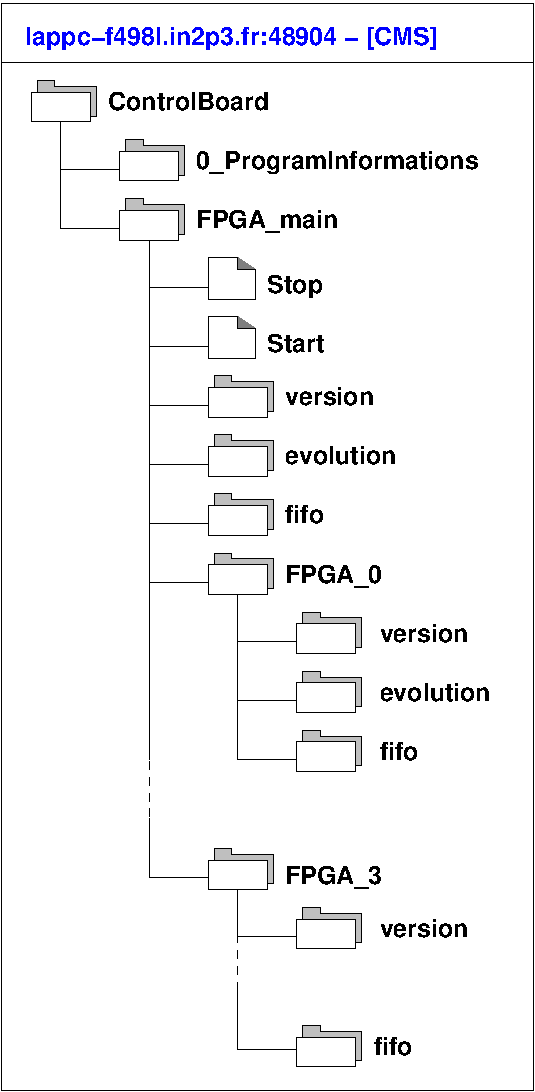
\includegraphics[width=5cm]{appendix/images/MOS_device_example_1.pdf}
\end{center}
\caption{Example of a  device managed through a MOS  server.  The root
  device is named \texttt{ControlBoard}.  First level daughter devices
  are  \texttt{0\_ProgramInformations} and  \texttt{FPGA\_main}.  Here
  the          MOS/OPCUA          server          is          labelled
  \texttt{CMS}.}\label{fig:an:mos_dev_1}
\end{figure}

% TODO


\subsection{Integration of a new device in the Vire environment}

The Vire  API also implements a  mechanism to describe a  hierarchy of
devices.  This  mechanism is independant  of the  one used in  the MOS
system but can  be easily made compatible with it.   This means that a
MOS  hierarchy  of devices  can  be  represented  in Vire.   The  Vire
hierarchy of  devices can  be considered as  some kind  of filesystem,
each device  being a folder with  its unique path, as  shown on figure
\ref{fig:an:mos_dev_2}.   The \emph{methods}  associated to  a devices
(or a datapoint) can be considered as plain executable files stored in
the  device's folder  : they  constitute the  set of  \emph{resources}
associated to the device.


\begin{figure}[h]
\begin{center}
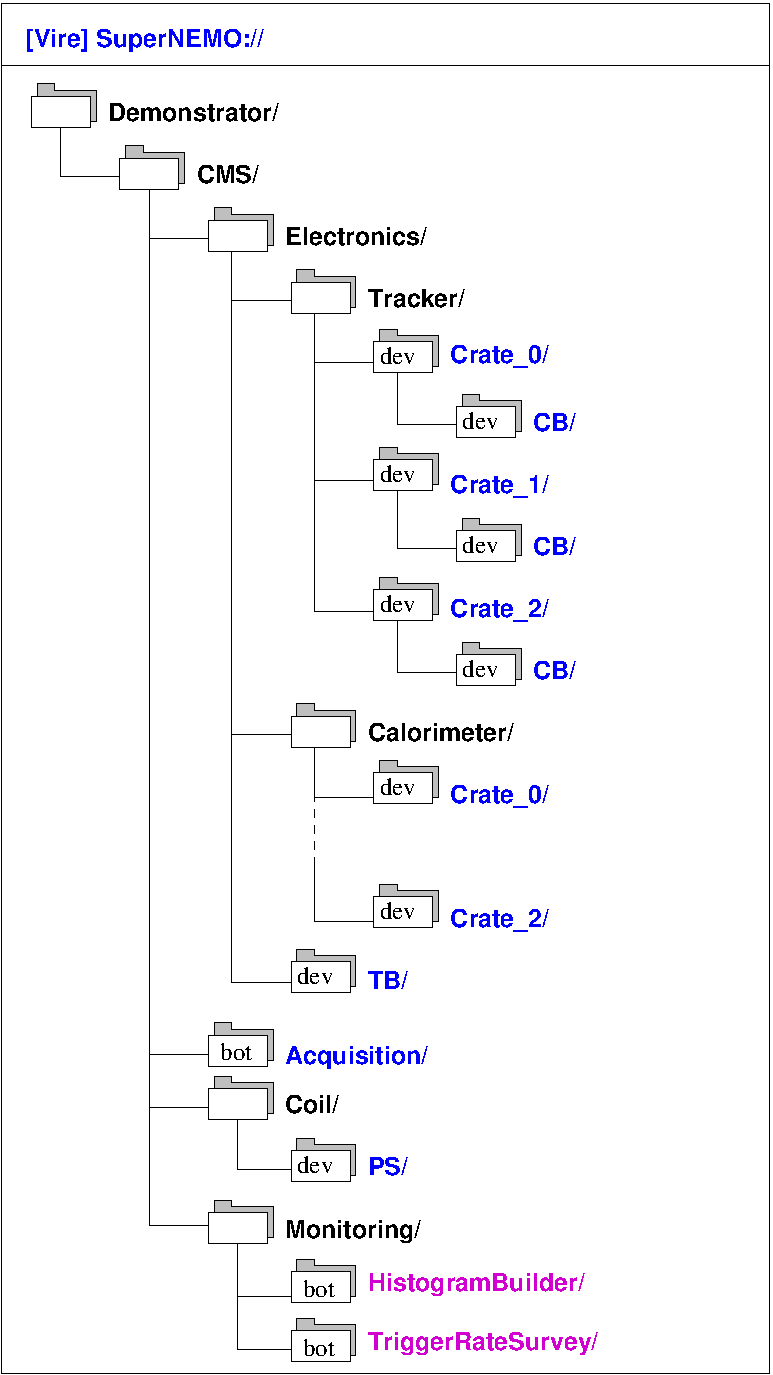
\includegraphics[width=5cm]{appendix/images/MOS_device_example_2.pdf}
\end{center}
\caption{Example of a hierarchy of  devices described by the Vire API.
  The root device is named  \texttt{SuperNEMO:}.  The top level (root)
  device  is  named  \texttt{Demonstrator}.  The  devices  colored  in
  \textcolor{blue}{blue}  are managed  through MOS/OPCUA.  The devices
  colored in \textcolor{magenta}{magenta} are directly embedded in the
  Vire server.  Devices with the \texttt{dev} tag are typical hardware
  device.  Devices  with the  \texttt{bot}  tag  are typical  software
  devices.   The  devices  colored in  \textbf{black}  are  structural
  pseudo-devices used to organize and  present a comprehensive view of
  the hierarchy. }\label{fig:an:mos_dev_2}
\end{figure}

The organisation of this hierarchy of devices is arbitrary and defined
by the designer of the  \emph{Control and Monitoring System}.  What is
important  to  understand  is  that  some  of  these  devices  can  be
associated  to  \emph{hardware  devices}  (a  power  supply  crate,  a
temperature probe\dots) and others  can be \emph{pseudo-devices}, i.e.
pure   software  object   (a   monitoring  robot,   a  file   transfer
daemon\dots).

In the context of the coupling of  the Vire server and the CMS server,
we are  in the event that  some devices are managed  by some MOS/OPCUA
servers and others are managed  in the Vire server itself.  Typically,
\emph{hardware devices}  are systematically managed through  the OPCUA
technology.  Vire has a mechanism to integrate such devices in its own
hierarchy.  This mechanism can  be considered like the \emph{mounting}
of   a   remote   filesystem   from  a   local   filesystem.    Figure
\ref{fig:an:mos_dev_0} illustrates  the case of many  hardware devices
-- managed by MOS -- that are integrated in the Vire system.  From the
Vire point of  view, the user does not see  the implementation details
for such  devices. He  does not  know the identity  of the  MOS server
hosting the device. He does not even know if the device is hosted by a
MOS server.  Devices are simply visible through the standard hierarchy
published by Vire with its  own device naming scheme, regardless their
true location.



\begin{figure}[h]
\begin{center}
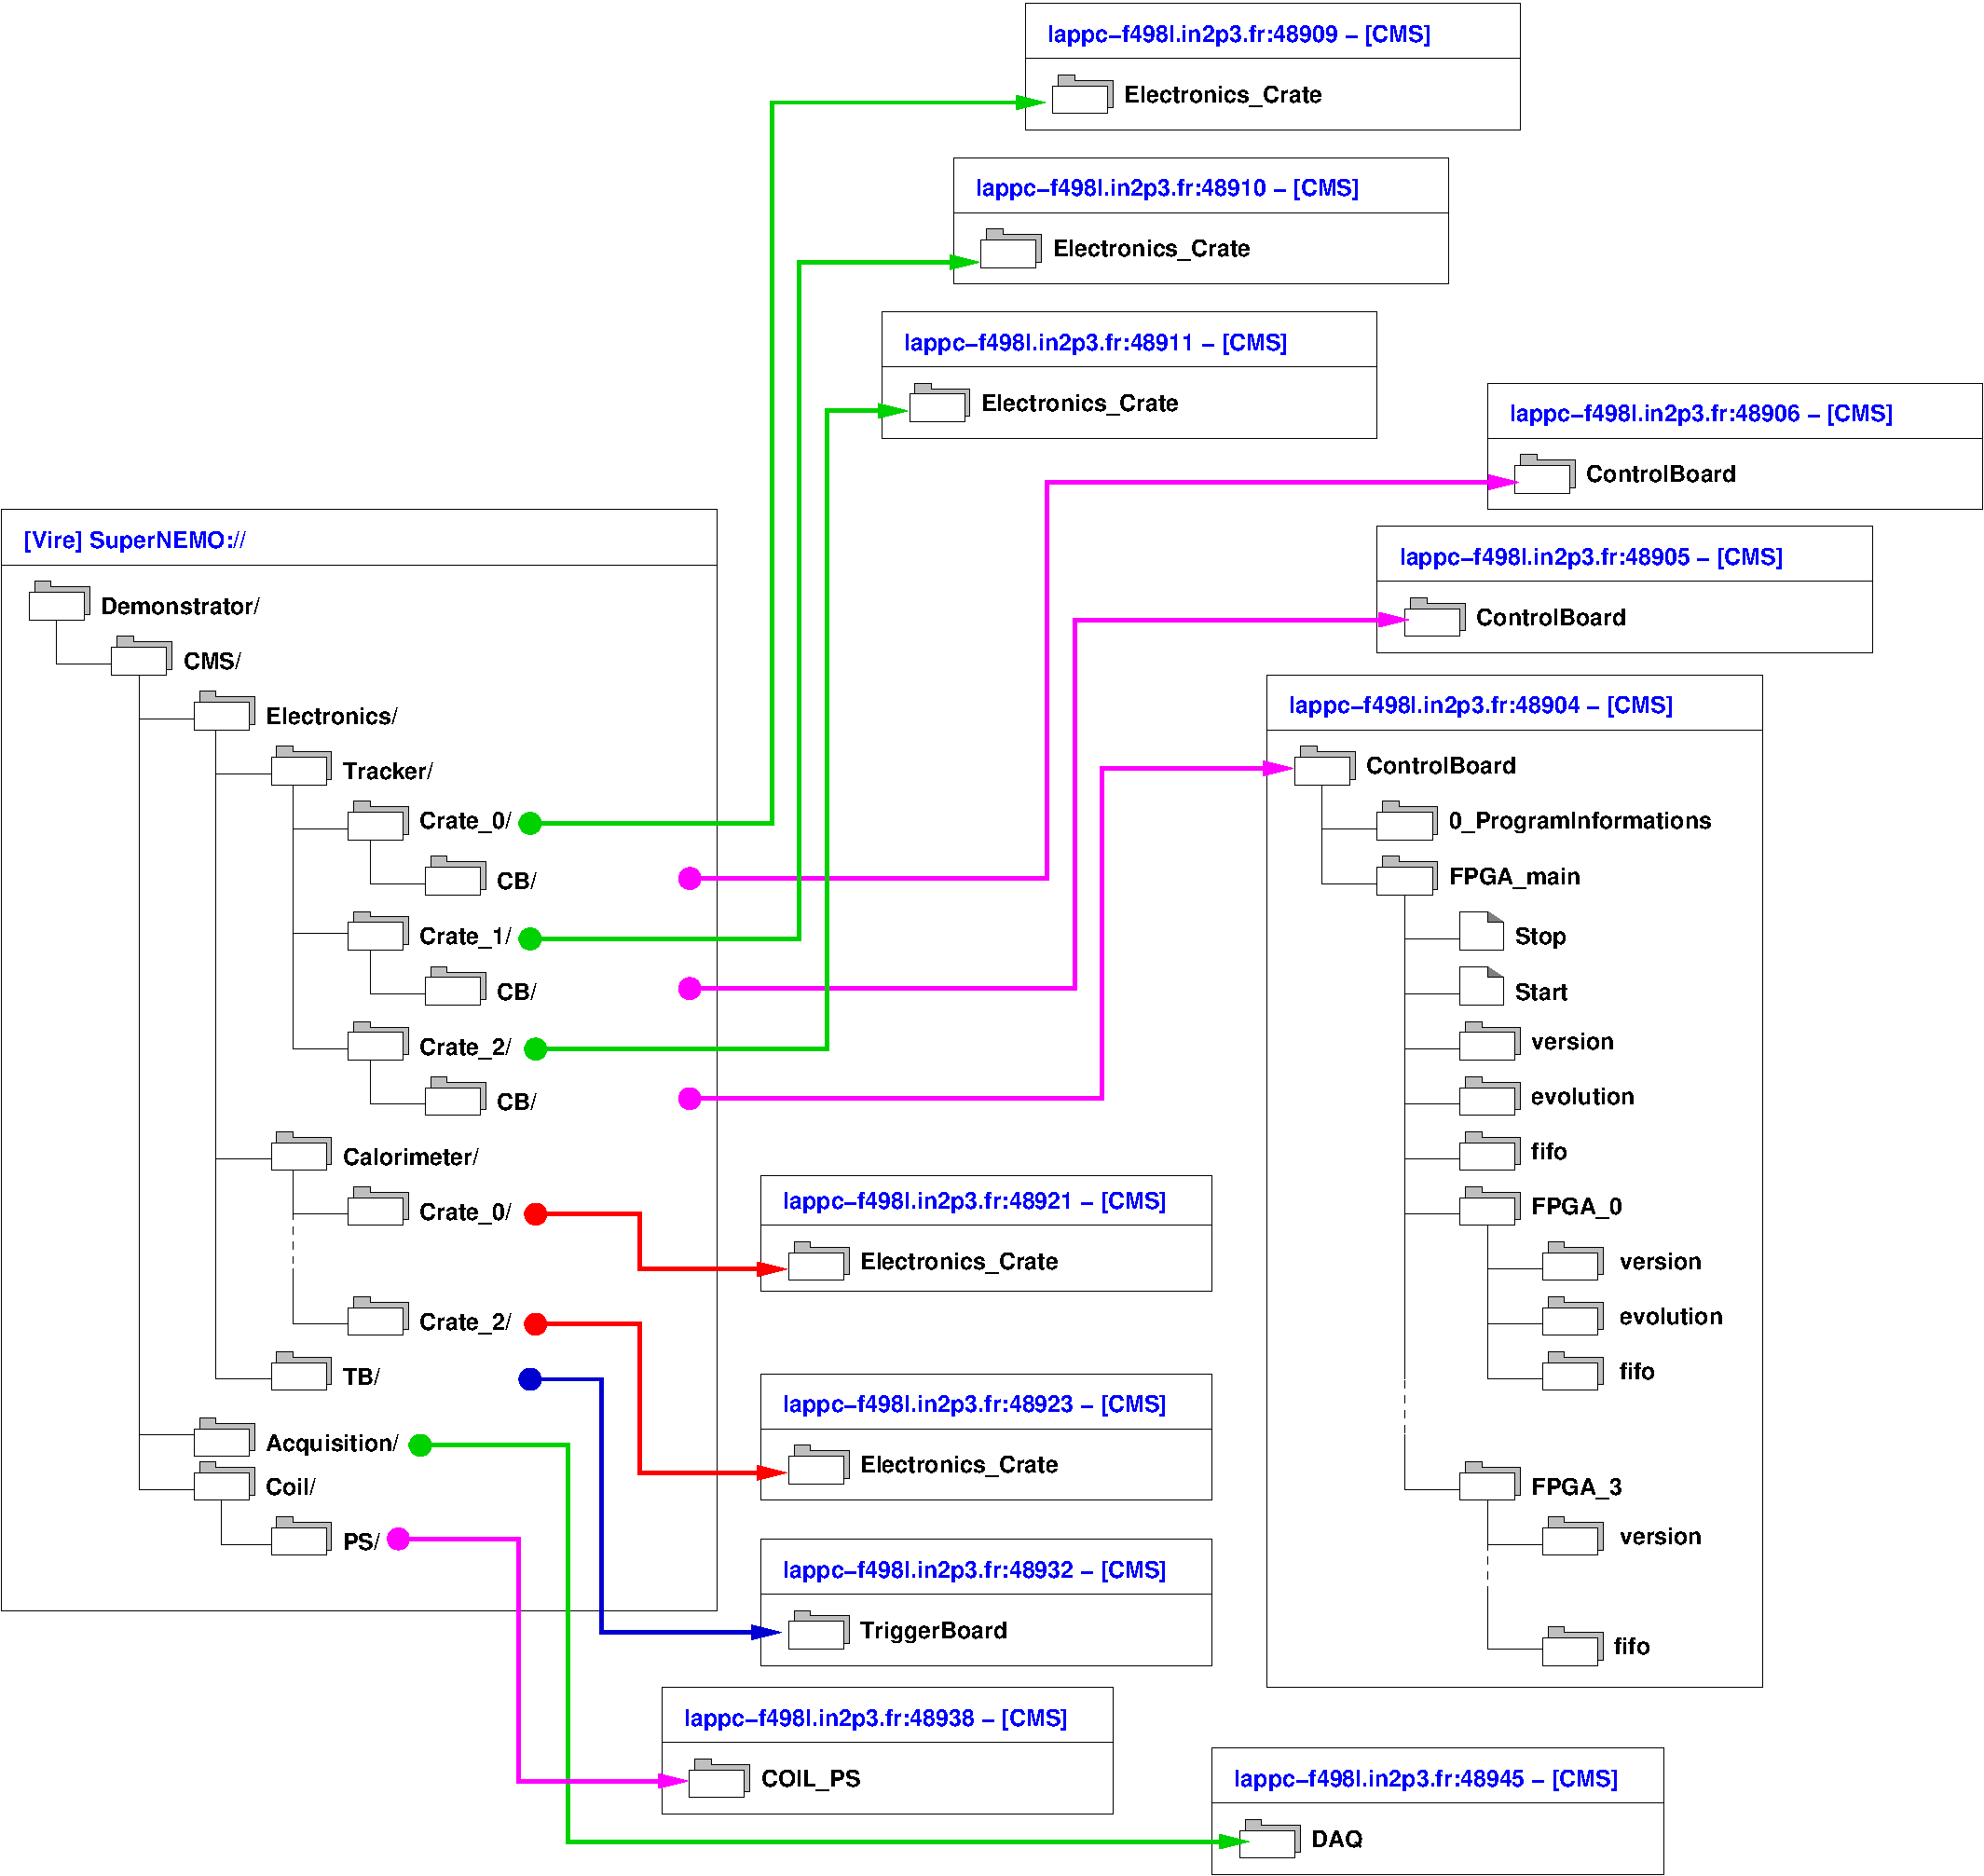
\includegraphics[width=\linewidth]{appendix/images/MOS_device_example_0.pdf}
\end{center}
\caption{The  mounting of  many  MOS device  hierarchies  in the  Vire
  device hierarchy.  Each OPCUA server  runs a simple  hardware device
  that is \emph{mounted} from a specific node with its own path.
%% of  devices described by the Vire API.
%%   The root device is named  \texttt{SuperNEMO:}.  The top level (root)
%%   device is  named \texttt{Demonstrator}. The devices  colored in blue
%%   are managed  through MOS/OPCUA. The  devices colored in  magenta are
%%   directly embedded in the Vire server.  Devices with the \texttt{dev}
%%   tag are typical  hardware device. Devices with  the \texttt{bot} tag
%%   are typical software devices.
}\label{fig:an:mos_dev_0}
\end{figure}




\subsection{Example}

Using  the examples  displayed  in  figure \ref{fig:an:mos_dev_0},  we
consider  in detail  the way  one specific  device managed  by MOS  is
mounted   in  the   Vire   hierarchy.  Figure   \ref{fig:an:mos_dev_3}
illustrates the mounting of a MOS device in Vire.

Here the Vire  server publishes the path of a  device representing the
control board  of the third  electronic crate  for the tracker  of the
SuperNEMO demonstrator module.  The full Vire path of this device is:

\textcolor{blue}{\texttt{SuperNEMO://Demonstrator/CMS/Electronics/Tracker/Crate\_2/CB}}

This is  the only Vire identifier  recognized by user to  address this
device.

On    the   figure,    one    can   see    that    the   MOS    server
\texttt{lappc−f498l.in2p3.fr} (port 48904) hosts a simple device which
is locally named \texttt{ControlBoard}.

When  mounting   this  device  in   the  Vire  hierarchy,   the  local
\texttt{[CMS]}  namespace and  \texttt{ControlBoard} device  names are
hidden and replaced by the Vire device path.  All daughter devices and
datapoints of  the \texttt{CMS/ControlBoard} device are  integrated as
daughters        of        the         Vire        device        named\\
\texttt{SuperNEMO://Demonstrator/CMS/Electronics/Tracker/Crate\_2/CB}.


For example, the \texttt{FPGA\_main} daughter device is now associated
to the following Vire path:

\textcolor{blue}{\texttt{SuperNEMO://Demonstrator/CMS/Electronics/Tracker/Crate\_2/CB/FPGA\_main/}}

and  its  \texttt{Stop} method  is  automatically  addressed with  the
following \emph{leaf} path:

\textcolor{blue}{\texttt{SuperNEMO://Demonstrator/CMS/Electronics/Tracker/Crate\_2/CB/FPGA\_main/Stop}}


\begin{figure}[h]
\begin{center}
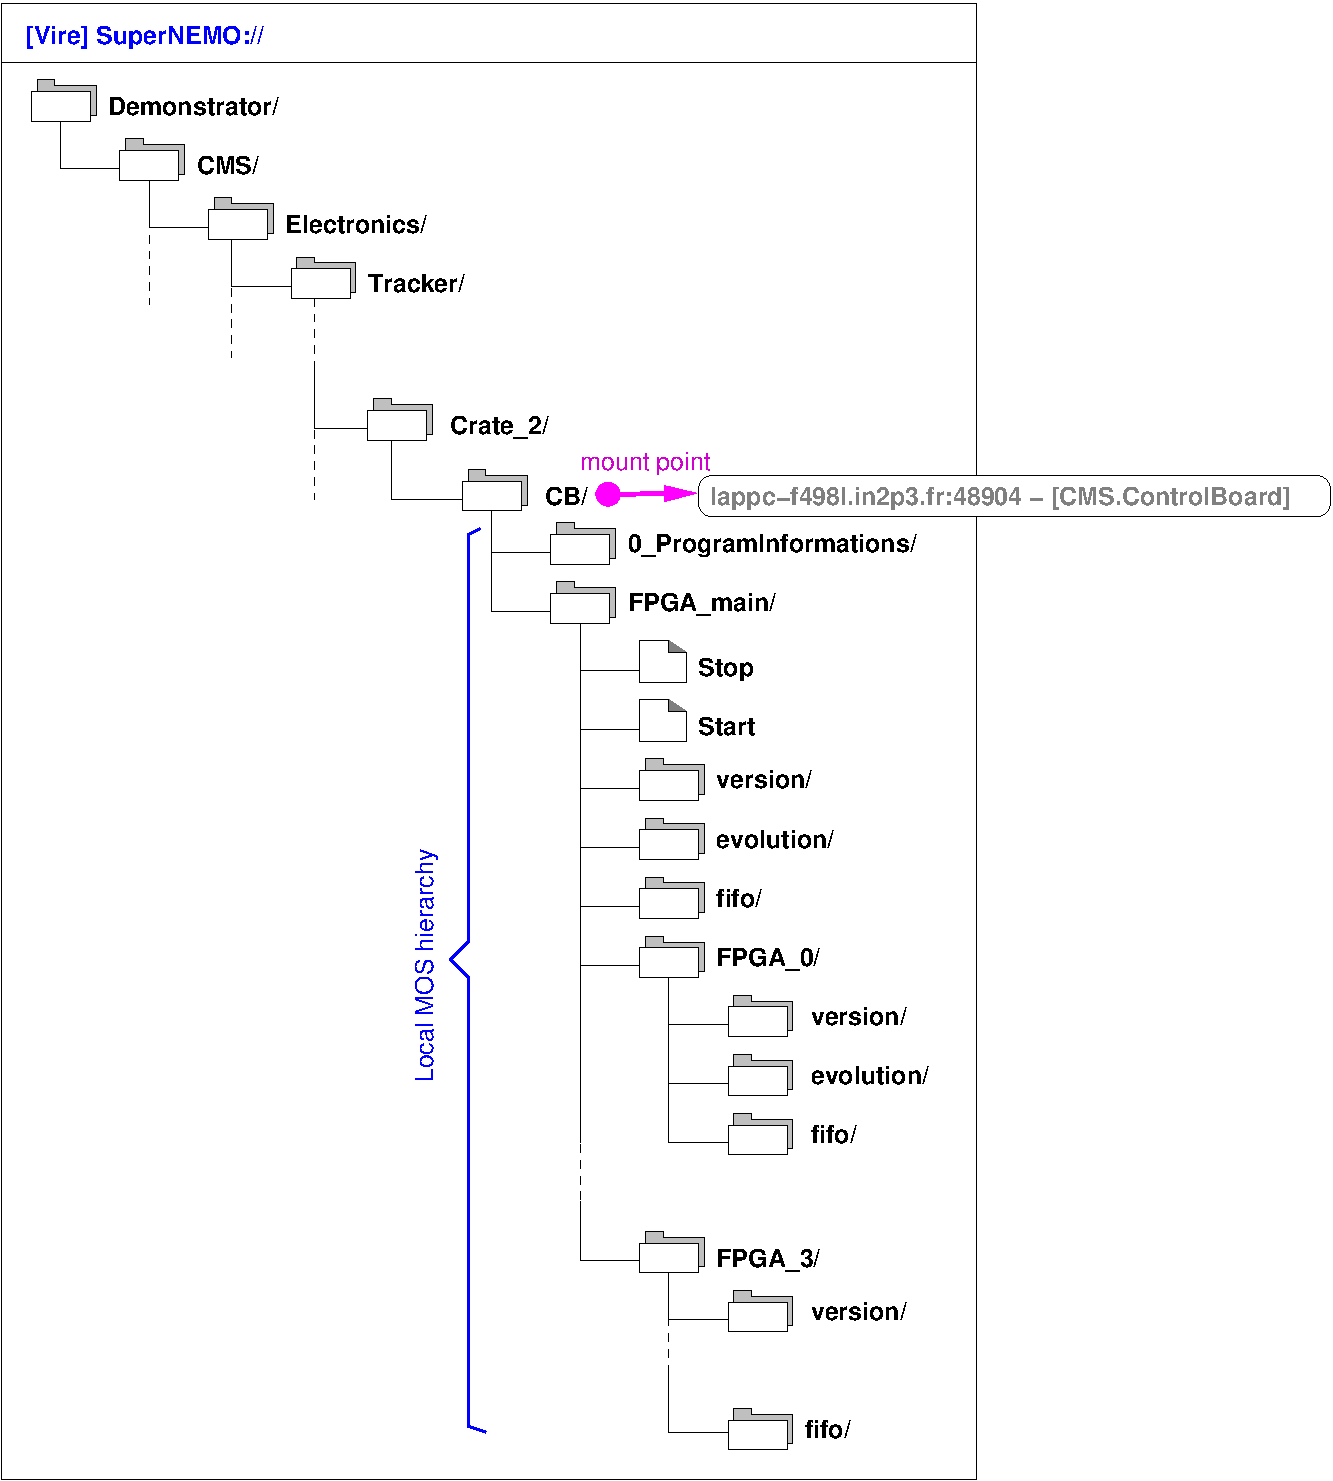
\includegraphics[width=0.8\linewidth]{appendix/images/MOS_device_example_3.pdf}
\end{center}
\caption{The  mounting of  one  MOS device and its local hierarchy  in the  Vire
  device hierarchy.}\label{fig:an:mos_dev_3}
\end{figure}



\subsection{Vire/MOS mapping}

As it can be  seen in the above example, the integration  of a new MOS
device in the Vire system is  achieved through soem kind of filesystem
mounting operation.   Particularly, it is  shown that the MOS  name of
the   mounted  root   device  is   replaced  by   an  arbitrary   Vire
path. However, all daughter  nodes (devices, datapoints) attached from
this root  node have their  relative MOS  names preserved in  the Vire
naming scheme.

Any  resource  (method)  associated  to any  of  such  daughter  nodes
inherits this relative naming scheme.

As Vire applications  describe resources through their  Vire paths, it
is thus needed to build an explicit map that associates resource paths
to MOS address  and name. The CMS  server will be able  to resolve the
MOS server/port and  embedded device associated to  the resource path.

The goal of the \texttt{devices\_launch.conf} file is not only to tell
the CMS server what MOS server should  be loaded and ran at start, but
also  to describe  the  \emph{mounting point/names}  used  by Vire  to
access the resources associated to MOS devices.  From the informations
stored in the  file, an explicit associative array must  be built when
the Vire server connect to the CMS server.  It will play the role of a
resource path resolver  when requests about resources will  be sent by
Vire applications.  This associative array  must be locked  during the
Vire/CMS connection.



%\subsubsection{Preparation of XML device models}

%% \noindent\underline{Pre-condition:}
%% The device is working and validated through the MOS/OPCUA server

%% \begin{enumerate}

%% \item Produce XML décrivant le modèle du device enrichi
%%   des metadata
%% Rédaction du fichier XML décrivant le modèle du device

%% \item Génération des fichiers model du type de device pour Vire

%% \item Génération des fichiers instances resolv.conf

%% \end{enumerate}


\vfill
\pagebreak
\clearpage

% end


\section{Vire messages}\label{app:vire_messages}

Within Vire  and between Vire  components and external  components, we
use  a communication  system  based on  Vire  messages.  This  section
describes the structure of such messages.

\subsection{General structure of a message}

Each message consists in two parts (figure \ref{fig-vire-message-message-cpp}):
\begin{itemize}

\item  the  \emph{header}  is   dedicated  to  generic  and  typicalle
  mandatory  informations  which  document   the  message  itself  and
  arbitrary high-level metadata.

\item  the \emph{body}  of the  message  contains the  real data: the payload.
  The structure of the message body depends on some convention. Vire uses
  its own convention to embed the payload data.

\end{itemize}

\begin{figure}[h]
\vskip 10pt
\small
\begin{Verbatim}[frame=single,xleftmargin=0.cm,label=\fbox{C++}]
struct vire::message::message {
  message_header header; // Header of the message
  message_body   body;   // Body of the message
};
\end{Verbatim}
\normalsize
\caption{The structure of a Vire message object (C++  class:
  \texttt{"vire::message::message"})}\label{fig-vire-message-message-cpp}
\end{figure}

\subsection{The message header}

The header contains (figure \ref{fig-vire-message-message_header-cpp}):
\begin{itemize}

  \item The mandatory \texttt{message\_id}  attribute is an identifier
    of the  message which  document the emitter  and a  unique message
    number.   Each emitter  is  responsible of  the  numbering of  the
    messages it  emits, typically using an  incremental technique. The
    message  number is  a positive  integer, starting  from 0  (figure
    \ref{fig-vire-message-message_identifier-cpp}).

  \item  The \texttt{timestamp}  attribute  encodes the  approximative
    time point when the message was  created. It contains the date and
    the time, using at least microsecond resolution.

    Typically,  with  JSON  encoding  system, it  is  expected  to  be
    formatted as a character string, using the following ISO format:

    \begin{center}
      \texttt{yyyymmddThhmmss.uuuuuu}
    \end{center}

    \noindent where:

    \vskip -10pt
    \begin{itemize}
    \item[\texttt{yyyymmdd} :] encodes year/month/day,
    \item[\texttt{hhmmssd} :] encodes hour/minute/second,
    \item[\texttt{uuuuuu} :] encodes microseconds.
    \end{itemize}

  \item   In   the   case    of   a   \emph{response}   message,   the
    \texttt{in\_reply\_to} attribute is set to identify the associated
    request message.

  \item  The \texttt{asynchronous}  boolean  attribute is  set if  the
    message processing  is explicitely requested  by the source  to be
    asynchronous (non-blocking).  In  RPC transactions, where requests
    are transmitted from one point to  the other, its default value is
    \emph{false}.   It  is possible  to  force  a RPC  transaction  in
    asynchronous mode.   This use  case is documented  elsewhere.  For
    event messaging, this flag is conventionally set to \emph{true}.

  \item  The  \texttt{body\_layout\_id}  attribute  is  the  mandatory
    identifier   of   the   layout   of  the   message   body   (class
    \texttt{"vire::utility::model\_identifier"}).  The  default layout
    for     message     body     inside    the     Vire     API     is
    \texttt{"vire::message::body\_format::typed\_payload"}, with version
    \texttt{"1.0"}                                             (figure
    \ref{fig-vire-utility-model_identifier-cpp}).

\end{itemize}


\begin{figure}[h]
\vskip 10pt
\small
\begin{Verbatim}[frame=single,xleftmargin=0.cm,label=\fbox{C++}]
struct vire::message::message_header {
  message_identifier message_id;     // Message identifier from the emitter.
  std::string        timestamp;      // Timestamp.
  message_identifier in_reply_to;    // Message identifier of the associated
                                     // request message (optional).
  bool               asynchronous,   // Asynchronous flag.
  vire::utility::model_identifier     body_layout_id; // Body layout identifier.
  std::map<std::string, std::string>  metadata;       // Key/value metadata dictionary.
};
\end{Verbatim}
\normalsize
\caption{The  structure  of  a   message  header  object  (C++  class:
  \texttt{"vire::message::message\_header"}).}\label{fig-vire-message-message_header-cpp}
\end{figure}

\begin{figure}[h]
\vskip 10pt
\small
\begin{Verbatim}[frame=single,xleftmargin=0.cm,label=\fbox{C++}]
struct vire::message::message_identifier {
  std::string emitter; // Name identifying the emitter of the message.
  int32_t     number;  // Number identifying the message in the emitter's
                       // message numbering scheme.
};
\end{Verbatim}
\normalsize
\caption{The      structure      of     a      message      identifier
  (C++  class:  \texttt{"vire::message::message\_identifier"}).}
\label{fig-vire-message-message_identifier-cpp}
\end{figure}

\begin{figure}[h]
\vskip 10pt
\small
\begin{Verbatim}[frame=single,xleftmargin=0.cm,label=\fbox{C++}]
struct vire::utility::model_identifier {
  std::string name;    // Name identifying the format of the message.
  std::string version; // String identifying the version of the format.
};
\end{Verbatim}
\normalsize
\caption{The structure of a model identifier (C++  class:  \texttt{"vire::utility::model\_identifier"}.}\label{fig-vire-utility-model_identifier-cpp}
\end{figure}




\begin{figure}[h]
\vskip 10pt
\small
\begin{Verbatim}[frame=single,xleftmargin=0.cm,label=\fbox{JSON}]
{
   "header" : {
      "message_id" : {
         "emitter" : "vire.server",
         "number" : 42
      },
      "timestamp" : "20160930T141408.413443",
      "in_reply_to" : {
         "initialized" : true,
         "value" : {
            "emitter" : "vire.client.0",
            "number" : 23
         }
      },
      "asynchronous" : false,
      "body_layout_id" : {
         "name" : "vire::message::body_format::typed_payload",
         "version" : {
            "initialized" : true,
            "value" : "1.0"
         }
      },
      "metadata" : [
         {
            "key" : "key1",
            "value" : "foo"
         },
         {
            "key" : "key2",
            "value" : "42"
         },
         {
            "key" : "key3",
            "value" : "3.1415899999999999"
         },
         {
            "key" : "key4",
            "value" : "true"
         }
      ]
   }
  "body" : {
      ...
   }
}
\end{Verbatim}
\normalsize
\caption{Example of  a   message  header  object in JSON format.}
\label{fig-vire-message-message_header-json}
\end{figure}

\vfill
\clearpage
\pagebreak

\subsection{The message body}

The    default    message   body    layout    in    Vire   is    named
\texttt{"vire::message::body\_format::typed\_payload"}        (version
\texttt{"1.0"}).   Each  message used  within  the  Vire framework  is
supposed to use this layout.  The general idea is that the body of the
message embeded the  \emph{payload object} that has  to be transmitted
between  two components  of  the system.   \emph{Payload objects}  are
classified in one of the three following categories:

\begin{enumerate}

\item \emph{Request}:  describes a request submitted  by one component
  to another component (generally during a synchronous RPC transaction).

\item  \emph{Response}: describes  the  response to  a former  request
  (generally during a synchronous RPC transaction).

\item \emph{Event}: describes an  arbitrary information record (alarm,
  exception, signal\dots) which is transmitted asynchronously.

\end{enumerate}

Vire implements the following class hierarchy:

\begin{center}
\begin{tikzpicture}
  \node (payload)  at (0,2)  [draw] {\texttt{vire::utility::base\_payload}};
  \node (request)  at (-4,0) [draw] {\texttt{vire::utility::base\_request}};
  \node (response) at (2,0)  [draw] {\texttt{vire::utility::base\_response}};
  \node (event)    at (8,0)  [draw] {\texttt{vire::utility::base\_event}};

  %\draw[style=help lines] (-3,-1) grid (10,4);
  \draw (node cs:name=response,anchor=north) |- (0,1);
  \draw (node cs:name=event,anchor=north)    |- (0,1);
  \draw[->] (node cs:name=request,anchor=north)
  |- (0,1) -| (node cs:name=payload,anchor=south);
\end{tikzpicture}
\end{center}

The requirements for the transmitted object are the following:

\begin{itemize}

\item The  type of the object  must be conventionally associated  to a
  unique     \emph{model      identifier}     object      (see     the
  \texttt{"vire::utility::model\_identifier"} class)  which contains a
  unique   name   (\textit{string    identifier})   and   possibly   a
  \textit{version identifier}.  Each software  component that may send
  or  receive the  object  should agree  on  this type  identification
  scheme.   This   enable  the  use  of   object  factories,  whatever
  programming  langage  is used  on  both  side of  the  communication
  system.

\item  For each  software component,  the object  type must  have some
  dedicated  encoding/decoding  functions  available  (again  whatever
  programming language is used). For example the Vire API supports the
  following encoding formats:

  \begin{itemize}

  \item JSON (MIME  encoding type: \texttt{"application/x-json"}), which
    is supportable by many languages,

  \item  Protobuf  (Google  Protocol   Buffers,  MIME  encoding  type:
    \texttt{"application/x-protobuf"}), which is also widely supported,

  \item   Boost/serialisation   (XML,    text   or   binary   archives
    \texttt{"application/x-boost-serialization-xml"},
    \texttt{"application/x-boost-serialization-text"},
    \texttt{"application/x-boost-serialization-binary"}),    which    in
    principle is supported by C++ only.

  \end{itemize}

  The Protobuf  encoding format will be  used to serialize/deserialize
  the  Vire  messages transported  between  the  Vire server  and  the
  CMS/LAPP server.

\end{itemize}

Vire uses a dedicated layout to represent the body of any message with
its embedded payload object. With this technique, the structure of the
body          contains         two          attributes         (figure
\ref{fig-app-vire-message-message_body-cpp}):

\begin{enumerate}

\item The \texttt{payload\_type\_id} specifies the type of the payload
  object   (figure   \ref{fig-app-vire-utility-model_identifier-cpp}).
  This unique name  is conventionaly fixed for a  given application. A
  version tag allows to support possible evolution of the object type.

\item The  \texttt{payload} is a  handle to  a payload object  of type
  request, response or event.

  %% \begin{itemize}
  %% \item Within  the producer  component of  the message,  the encoding
  %%   function associated to the object  type is responsible to generate
  %%   the JSON stream for the object and store it in the buffer.

  %% \item Within  the consumer  component of  the message,  the decoding
  %%   function associated to the object type is responsible to parse the
  %%   JSON stream stored in the buffer and restore the object in memory.

  %% \end{itemize}

  It is expected  that, on both sides of the  connection, the software
  components can  access dedicated  software plugins which  ensure the
  support  of  various   \emph{payload  object  types}  conventionnaly
  associated  with  their  \emph{payload type  identifiers}  and  also
  providing JSON and/or Protobuf encoding/decoding functionalities.

  %% The   system  allows  to  support
  %% modification  in the  structure of  the objects  thanks to  version
  %% tagging.

\end{enumerate}

\begin{figure}[h]
\vskip 10pt
\small
\begin{Verbatim}[frame=single,xleftmargin=0.cm,label=\fbox{C++}]
struct message_body {
  vire::utility::model_identifier     payload_type_id; // Object type identifier.
  const vire::utility::base_payload * payload;         // Handle to a payload object.
};
\end{Verbatim}
\normalsize
\caption{The structure of a message body object (C++).}
\label{fig-app-vire-message-message_body-cpp}
\end{figure}

\begin{figure}[h]
\vskip 10pt
\small
\begin{Verbatim}[frame=single,xleftmargin=0.cm,label=\fbox{JSON}]
{
  "header" : {
    ...
  },
  "body" : {
    "payload_type_id" : {
      "name" : "vire::message::testing::error_event",
      "version" : {
        "initialized" : false
      }
    },
    "payload" : {
      "timestamp" : "20160930T141743.759085"
      "err" : {
        "code" : 3,
        "message" : "A basic error"
      },
    }
  }
}
\end{Verbatim}
\normalsize
\caption{Example of  a   message  body  object in JSON format.}
\label{fig-vire-message-message_body-json}
\end{figure}

\vfill
\clearpage
\pagebreak

% end

%\input{appendix/app_json_fmt.tex}

\section{The \emph{Protocol Buffers} format}\label{app:protobuf_fmt}

\subsection{Introduction}

The  Google  Protocol Buffers  (\emph{protobuf})  library  is used  to
represent the objects that are exchanged between the Vire clients, the
Vire server and the CMS server.  The  version 3 of the format is used,
implying   at   least   version   3.0.0  (September   2016)   of   the
\emph{protobuf} library.

Each  data   structure  of  interest   can  be  described   through  a
\texttt{.proto}  file  from  which  stub files  can  be  automatically
generated  with the  \texttt{protoc} compiler.  For Vire  and its  CMS
interface, the C++ and Java programming languages will be used.


A  collection of  \texttt{.proto}  files are  provided  with the  Vire
library to represent all kind  of data structures transferable between
networked agents  (Vire server,  Vire clients, CMS/LAPP  server).  The
objects of  the highest level  are named \emph{payload  objects} (like
\emph{request},  \emph{response} and  \emph{event} objects).   They
are composed of attributes of more basic data structures.

\subsection{Example}

The following  class diagram  illustrates two data  structures defined
within the Vire library with an inheritance relationship between them.

\begin{center}
  \begin{tikzpicture}
    \node (base)     at (0,1.5)  [draw] {\texttt{vire::utility::base\_error}};
    \node (setup)    at (0,0)  [draw] {\texttt{vire::utility::invalid\_setup\_id\_error}};

    \draw[->]   (node cs:name=setup,anchor=north) |- (0,1);
    |- (0,1) -| (node cs:name=base,anchor=south);
  \end{tikzpicture}
\end{center}

The \texttt{vire::utility::base\_error}  is the  parent class  for all
\emph{error}  objects.   It  contains   two  attributes:   an  integer
\emph{error code}  and a  character string describing  the \emph{error
  message}.

The   \texttt{vire::utility::invalid\_setup\_id\_error}  class   is  a
specialized error class  which represents explicitely an  error due to
an identification  failure of  the experimental setup.   It implements
additional mutually exclusive attributes: the \emph{unrecognized name}
of the setup or the \emph{unrecognized version} of the setup.

This   example  illustrates   the  protobuf   representation  of   the
\texttt{vire::utility::base\_error}  in the  Vire  library, using  the
\texttt{"vire/utility/BaseError.proto"} file:

\small
\begin{Verbatim}[frame=single,xleftmargin=0.cm,label=\fbox{protobuf}]
  syntax = "proto3";
  package vire.utility; // Namespace

  message BaseError {

    // reserved 1; // Reserved for _base message

    // Attributes:
    int32  code           = 100; // The error code
    string message_format = 101; // The error description message

  }
\end{Verbatim}
\normalsize

\vfill
\clearpage
\pagebreak

\subsection{Vire protobuf conventions}

Vire uses the following conventions:

\begin{enumerate}

\item
  The member index  \texttt{1} is reserved to represent the  link of a
  class to its main base/parent class (if any).  It is not used if the
  data structure does not inherit any data structure.
  If a data structure naturally inherits another one, it is thus possible
  to  represent the  inheritance  relationship as  illustrated with  the
  \texttt{"vire/utility/InvalidSetupIdError.proto"}      file      which
  represents the \texttt{vire::utility::invalid\_setup\_id\_error} class
  in the Vire library:

  \small
  \begin{Verbatim}[frame=single,xleftmargin=0.cm,label=\fbox{protobuf}]
    syntax = "proto3";
    package vire.utility; // Namespace

    import "vire/utility/BaseError.proto"; // Dependency

    message InvalidSetupIdError {

      BaseError _base = 1; // The base class

      // Additional attributes:
      oneof detail { // Mutual exclusion
        string invalid_setup_name    = 100; // The failed setup name
        string invalid_setup_version = 101; // The failed setup version
      }

    }
  \end{Verbatim}
  \normalsize

\item The  \texttt{\_base} member  is conventionally  used to  represent the
  inheritance   relationship    from   a   data   structure    of   type
  \texttt{"vire.utility.BaseError"}.

\item Member indexes from \texttt{2}  to \texttt{99} are also reserved
  for possible future usage (multiple inheritance, metadata\dots).

\item
  The first member of the data structure must start at index \texttt{100}.

\end{enumerate}

\vfill
\clearpage
\pagebreak

% end


\section{Vire payload objects}\label{app:payload}

\subsection{Introduction}

As  mentioned in  appendix \ref{app:protobuf_fmt},  Vire messages  are
wrappers for \emph{payload objects}.  Each  type of payload object can
be represented  through the \emph{protobuf} mechanism.   The following
class hierarchy shows the base architecture used to define new payload
objects.

\begin{center}
\begin{tikzpicture}
  \node (payload)  at (0,2)   [draw] {\texttt{vire::utility::base\_payload}};
  \node (request)  at (-4,0)  [draw] {\texttt{vire::utility::base\_request}};
  \node (response) at (2,0)   [draw] {\texttt{vire::utility::base\_response}};
  \node (event)    at (8,0)   [draw] {\texttt{vire::utility::base\_event}};
  \node (my)       at (-4,-2) [draw] {\texttt{my\_request}};
  \node (your)     at (2,-2)  [draw] {\texttt{your\_response}};
  \node (its)    at (8,-2)    [draw] {\texttt{its\_alarm}};

  %\draw[style=help lines] (-6,-2) grid (10,2);
  \draw (node cs:name=response,anchor=north) |- (0,1);
  \draw (node cs:name=event,anchor=north)    |- (0,1);
  \draw[->] (node cs:name=request,anchor=north)
  |- (0,1) -| (node cs:name=payload,anchor=south);
  \draw[->] (node cs:name=my,anchor=north)
  |- (-4,-1) -| (node cs:name=request,anchor=south);
  \draw[->] (node cs:name=your,anchor=north)
  |- (2,-1) -| (node cs:name=response,anchor=south);
  \draw[->] (node cs:name=its,anchor=north)
  |- (8,-1) -| (node cs:name=event,anchor=south);
\end{tikzpicture}
\end{center}


\begin{center}
\vskip 10pt
\small
\begin{tabular}{|l|l|l|}
  \hline
  \textbf{Vire C++ class} & \textbf{protobuf message type} & \textbf{protobuf definition file} \\
  \hline
  \hline
  \multicolumn{3}{|c|}{\emph{general types}} \\
  \hline
  boost::posix\_time::ptime & google.protobuf.Timestamp & google/protobuf/timestamp.proto \\
  \hline
  \hline
  \multicolumn{3}{|c|}{\emph{identifier types}} \\
  \hline
  vire::utility::base\_identifier & vire.utility.Baseidentifier & vire/utility/Baseidentifier.proto \\
  \hline
  vire::utility::instance\_identifier & vire.utility.InstanceIdentifier & vire/utility/InstanceIdentifier.proto \\
  \hline
  vire::utility::model\_identifier & vire.utility.ModelIdentifier & vire/utility/ModelIdentifier.proto \\
  \hline
  \hline
  \multicolumn{3}{|c|}{\emph{error types}} \\
  \hline
  vire::utility::base\_error & vire.utility.BaseError & vire/utility/BaseError.proto \\
  \hline
  vire::utility::invalid\_context\_error & vire.utility.InvalidContextError & vire/utility/InvalidContextError.proto \\
  \hline
  vire::utility::invalid\_setup\_id\_error & vire.utility.InvalidSetupIdError & vire/utility/InvalidSetupIdError.proto \\
  \hline
  \hline
  \multicolumn{3}{|c|}{\emph{payload types}} \\
  \hline
  vire::utility::base\_payload & vire.utility.BasePayload & vire/utility/BasePayload.proto \\
  \hline
  vire::utility::base\_request & vire.utility.BaseRequest & vire/utility/BaseRequest.proto \\
  \hline
  vire::utility::base\_response & vire.utility.BaseResponse & vire/utility/BaseResponse.proto \\
  \hline
  vire::utility::base\_event & vire.utility.BaseEvent & vire/utility/BaseEvent.proto \\
  \hline
  vire::utility::base\_alarm & vire.utility.BaseAlarm & vire/utility/BaseAlarm.proto \\
  \hline
  \hline
  \multicolumn{3}{|c|}{\emph{messenging types}} \\
  \hline
  vire::message::message\_identifier & vire.message.MessageIdentifier & vire/message/MessageIdentifier.proto \\
  \hline
  vire::message::msg\_header & vire.message.MsgHeader & vire/message/MsgHeader.proto \\
  \hline
  vire::message::msg\_body & vire.message.MsgBody & vire/message/MsgBody.proto \\
  \hline
  vire::message::message & vire.message.Message & vire/message/Message.proto \\
  \hline
\end{tabular}
\normalsize
\end{center}


\begin{center}
\vskip 10pt
\small
\begin{tabular}{|l|l|l|}
  \hline
  \multicolumn{3}{|c|}{\emph{Resource management related types}} \\
  \hline
  vire::cms::resource\_status\_record & vire.cms.ResourceStatusRecord & vire/cms/ResourceStatusRecord.proto \\
  \hline
  vire::cms::resource\_fetch\_status\_request & vire.cms.ResourceFetchStatusRequest & vire/cms/ResourceFetchStatusRequest.proto \\
  \hline
  vire::cms::resource\_fetch\_status\_success\_response & vire.cms.ResourceFetchStatusSuccessResponse & vire/cms/ResourceFetchStatusSuccessResponse.proto \\
  \hline
  vire::cms::resource\_fetch\_status\_failure\_response & vire.cms.ResourceFetchStatusFailureResponse & vire/cms/ResourceFetchStatusFailureResponse.proto \\
  \hline
  vire::cms::resource\_exec\_request & vire.cms.ResourceExecRequest & vire/cms/ResourceExecRequest.proto \\
  \hline
  vire::cms::resource\_exec\_success\_response & vire.cms.ResourceExecSuccessResponse & vire/cms/ResourceExecSuccessResponse.proto \\
  \hline
  vire::cms::resource\_exec\_failure\_response & vire.cms.ResourceExecFailureResponse & vire/cms/ResourceExecFailureResponse.proto \\
  \hline
  vire::cms::resource\_exec\_non\_blocking\_request & vire.cms.ResourceExecNonBlockingRequest & vire/cms/ResourceExecNonBlockingRequest.proto \\
  \hline
  vire::cms::resource\_exec\_non\_blocking\_ack\_response & vire.cms.ResourceExecNonBlockingAckResponse & vire/cms/ResourceExecNonBlockingAckResponse.proto \\
  \hline
  vire::cms::resource\_exec\_non\_blocking\_noack\_response & vire.cms.ResourceExecNonBlockingNoackResponse & vire/cms/ResourceExecNonBlockingNoackResponse.proto \\
  \hline
  vire::cms::resource\_exec\_non\_blocking\_success\_event & vire.cms.ResourceExecNonBlockingSuccessEvent & vire/cms/ResourceExecNonBlockingSuccessEvent.proto \\
  \hline
  vire::cms::resource\_exec\_non\_blocking\_failure\_event & vire.cms.ResourceExecNonBlockingFailureEvent & vire/cms/ResourceExecNonBlockingFailureEvent.proto \\
  \hline
  vire::cms::resource\_exec\_error & vire.cms.ResourceExecError & vire/cms/ResourceExecError.proto \\
  \hline
  vire::cms::invalid\_status\_error & vire.cms.ResourceExecError & vire/cms/ResourceExecError.proto \\
  \hline
  %% vire::cms::invalid\_credentials\_error & vire.cms.InvalidCredentialsError & vire/cms/InvalidCredentialsError.proto \\
  %% \hline
  %% vire::cms::invalid\_user\_error & vire.cms.InvalidUserError & vire/cms/InvalidUserError.proto \\
  %% \hline
  vire::cms::invalid\_resource\_error & vire.cms.InvalidUserError & vire/cms/InvalidUserError.proto \\
  \hline
  vire::cms::no\_pubsub\_resource\_error & vire.cms.NoPubsubResourceError & vire/cms/NoPubsubResourceError.proto \\
  \hline
  \hline
  \multicolumn{3}{|c|}{\emph{Resource pub/sub management types}} \\
  \hline
  vire::cms::resource\_pubsub\_subscribe\_request & vire.cms.ResourcePubsubSubscribeRequest & vire/cms/ResourcePubsubSubscribeRequest.proto \\
  \hline
  vire::cms::resource\_pubsub\_subscribe\_success\_response & vire.cms.ResourcePubsubSubscribeRSuccessResponse & vire/cms/ResourcePubsubSubscribeRSuccessResponse.proto \\
  \hline
  vire::cms::resource\_pubsub\_subscribe\_failure\_response & vire.cms.ResourcePubsubSubscribeRFailureResponse & vire/cms/ResourcePubsubSubscribeRSuccessResponse.proto \\
  \hline
  \hline
  \multicolumn{3}{|c|}{\emph{Vire/CMS server interface types}} \\
  \hline
  vire::cmsinterface::connection\_request & vire.cmsinterface.ConnectionRequest & vire/cmsinterface/ConnectionRequest.proto \\
  \hline
  vire::cmsinterface::connection\_success\_response & vire.cmsinterface.ConnectionSuccessResponse & vire/cmsinterface/ConnectionSuccessResponse.proto \\
  \hline
  vire::cmsinterface::connection\_failure\_response & vire.cmsinterface.ConnectionFailureResponse & vire/cmsinterface/ConnectionFailureResponse.proto \\
  \emph{embedded:} unknown\_resources\_error & .UnknownResourcesError &  \\
  \hline
  vire::cmsinterface::disconnection\_request & vire.cmsinterface.DisconnectionRequest & vire/cmsinterface/DisconnectionRequest.proto \\
  \hline
  vire::cmsinterface::disconnection\_success\_response & vire.cmsinterface.DisconnectionSuccessResponse & vire/cmsinterface/DisconnectionSuccessResponse.proto \\
  \hline
  %% \hline
  %% vire::cmsinterface::disconnection\_failure\_response & vire.cmsinterface.DisconnectionFailureResponse & vire/cmsinterface/DisconnectionFailureResponse.proto \\
\end{tabular}
\normalsize
\end{center}

\subsection{Basic data structures}

Any  payload object  (request, response  or event)  generally contains
some information records which are  specific to the functionalities of
the  payload  object they  belong.   These  records are  of  arbitrary
types. Of course they should be  translatable in terms of the protobuf
library.
%Of course they can be (de)serialized using JSON.
Some of these types are very  general and defined within the Vire core
API itself because they are reused by various payload objects not only
through  the Vire-CMS/LAPP  interface  but also  between  Vire clients  and
servers, independently  of the  CMS/LAPP server.  However,  the use  of the
Protocol Buffers interface makes possible  to publish the interface of
such data to the outside world, including the CMS/LAPP server in priority.

%% Other one are specific to the Vire/CMS interface and thus managed only
%% in the \texttt{Vire\_CMSInterface} API.
These  types  are considered  as  \emph{basic}.  Among them  we  find:
generic error  types, generic  identifier types,  timestamps, resource
status records\dots We propose to describe them in this section.

Once a sufficient collection of  basic data record types is available,
it  is possible  to describe  high  level payload  object types  which
aggregate attributes of such types.

Other record  types are specific to  some payload objects and  will be
never  used outside  the scope  of these  payload objects.   Such data
structures will be  explicitely declared with the  payload object they
belong to, likely as embedded types/classes.


\subsubsection{Errors}

Some  \emph{response} or  \emph{event} payload  objects may  contain a
specific  error  record  object.   A  \emph{failure  response}  or  an
\emph{exception  event}  object will  generally  embed  such an  error
record object.

Each  \emph{error record}  is represented  by an  instance of  a given
error type.   Each of  the error  types defined  in Vire  inherits the
\texttt{vire::utility::base\_error}      base       class      (figure
\ref{fig-app-payload-base_error})   which   contains   the   following
attributes:

\begin{itemize}

\item the error code: A non zero  integer which is set to 1 by default
  (indicating  a  generic  failure  case).   The  error  code  can  be
  conventionally  set to  any positive  integer value  to represent  a
  specific error case, depending on the context.

\item the error  message: an optional human  readable character string
  which documents the error as usefully as possible.

\end{itemize}

\begin{figure}[h]
\vskip 10pt
\small
\begin{Verbatim}[frame=single,xleftmargin=0.cm,label=\fbox{C++}]
struct vire::utility::base_error
{
  // Attributes:
  int         code;           // Error code (>0).
  std::string message_format; // Error message (optional).
};
\end{Verbatim}
\normalsize
\caption{The structure of a \texttt{"vire::utility::base\_error"} object
  (C++).}
\label{fig-app-payload-base_error}
\end{figure}


%% An example of JSON formatted basic error object is given in figure
%% \ref{fig-app-payload-base_error-1}.
%%
%% \begin{figure}[h]
%% \vskip 10pt
%% \small
%% \begin{Verbatim}[frame=single,xleftmargin=0.cm,label=\fbox{\texttt{JSON}}]
%% {
%%   "code" : "42",
%%   "message_format" : "Invalid AMQP server port=[2341]"
%% }
%% \end{Verbatim}
%% \normalsize
%% \caption{JSON  formatted  basic  error  object  (class
%%   \texttt{vire::utility::base\_error}.}
%% \label{fig-app-payload-base_error-1}
%% \end{figure}

Several type of generic errors are defined in Vire:


\begin{center}
\begin{tikzpicture}
  \node (base)     at (0,2)  [draw] {\texttt{vire::utility::base\_error}};
  \node (context)  at (-4,0) [draw] {\texttt{vire::utility::invalid\_context\_error}};
  \node (setup)    at (0,-1)  [draw] {\texttt{vire::utility::invalid\_setup\_id\_error}};
  \node (resource) at (4,0)  [draw] {\texttt{vire::cms::invalid\_resource\_error}};
  \node (user)     at (8,-1)  [draw] {\texttt{vire::cms::invalid\_user\_error}};

  \draw     (node cs:name=setup,anchor=north)    |- (0,1);
  \draw     (node cs:name=resource,anchor=north) |- (0,1);
  \draw     (node cs:name=user,anchor=north)     |- (0,1);
  \draw[->] (node cs:name=context,anchor=north)
  |- (0,1) -| (node cs:name=base,anchor=south);
\end{tikzpicture}
\end{center}

\noindent
Here are a few error object types defined in Vire.  Some types belongs
to the \texttt{utility} namespace, other  ones are in the \texttt{cms}
namespace:

\begin{itemize}

\item \texttt{"vire::utility::invalid\_context\_error"} : occurs typically when
  the general context of the execution of a given resource is not adapted.\\
  It is mapped to the \texttt{"vire.utility.InvalidContextError"} protobuf record.

\item \texttt{"vire::utility::invalid\_setup\_id\_error"} : occurs in case
  of an invalid identification of the experimental setup managed
  by the Vire or CMS server.\\
  It is mapped to the \texttt{"vire.utility.InvalidSetupIdError"} protobuf record.

\item \texttt{"vire::cms::invalid\_resource\_error"} : occurs in case
  of an invalid identification of a resource.\\
  It is mapped to the  \texttt{"vire.cms.InvalidResourceError"} protobuf record.

\item \texttt{"vire::cms::invalid\_status\_error"}: occurs when an attempt
  to access a resource that has not the proper status.\\
  It is mapped to the  \texttt{"vire.cms.InvalidStatusError"} protobuf record.

\item \texttt{"vire::cms::invalid\_user\_error"} : occurs in case
  of an invalid identification of an user.\\
  It is mapped to the  \texttt{"vire.cms.InvalidUserError"} protobuf record.

\item \texttt{"vire::cms::invalid\_credentials\_error"} : occurs in case
  of user authentication error.\\
  It is mapped to the  \texttt{"vire.cms.InvalidCredentialsError"} protobuf record.

\item \texttt{"vire::cms::resource\_exec\_error"} : occurs in case
  of error at the execution of a given resource.\\
  It is mapped to the  \texttt{"vire.cms.ResourceExecError"} protobuf record.

\end{itemize}



\subsubsection{Object and type identifiers}

Vire  uses  some dedicated  classes  to  represent the  identifier  of
various objects  (or \emph{instances})  as well  as various  types (or
\emph{models})  of components.  Vire  implements  the following  class
hierarchy:

\begin{center}
\begin{tikzpicture}
  \node (base)  at (0,2)  [draw] {\texttt{vire::utility::base\_identifier}};
  \node (instance)  at (-4,0) [draw] {\texttt{vire::utility::instance\_identifier}};
  \node (model) at (4,0)  [draw] {\texttt{vire::utility::model\_identifier}};

  \draw (node cs:name=model,anchor=north) |- (0,1);
\draw[->] (node cs:name=instance,anchor=north)
  |- (0,1) -| (node cs:name=base,anchor=south);
\end{tikzpicture}
\end{center}

The          \texttt{vire::utility::base\_identifier}          (figure
\ref{fig-app-payload-base_identifier}) class is  a pure abstract class
that cannot be instantiated. However  it contains a mandatory name and
an  optional  version description  which  are  used by  all  inherited
classes:

\begin{itemize}

\item The   \texttt{vire::utility::instance\_identifier}    concrete   class
inherits  \texttt{vire::utility::base\_identifier}  and   is  used  to
identify \underline{unique instances of objects} known by the system.

\item The  \texttt{vire::utility::model\_identifier}   concrete  class  also
inherits  \texttt{vire::utility::base\_identifier}  and   is  used  to
identify \underline{types of objects} registered in the system.

\end{itemize}

The only difference between these two classes is the validation scheme
of  the name  attribute.

\begin{figure}[h]
\vskip 10pt
\small
\begin{Verbatim}[frame=single,xleftmargin=0.cm,label=\fbox{C++}]
struct base_identifier
{
  // Attributes:
  std::string name;    // The mandatory name uniquely identifying the object or
                       // the type of object.
  std::string version; // An optional character string representing the version
                       // of the object type.
};
\end{Verbatim}
\normalsize
\caption{The structure of the \texttt{vire::utility::base\_identifier}
  class (C++).}
\label{fig-app-payload-base_identifier}
\end{figure}

%%  Figure  \ref{fig-app-payload-identifier-json}
%% shows an example of instance indentifier.
%% \begin{figure}[h]
%% \vskip 10pt
%% \small
%% \begin{Verbatim}[frame=single,xleftmargin=0.cm,label=\fbox{\texttt{JSON}}]
%% {
%%   "name" : "vire::resource::invalid_resource_error",
%%   "version" : "1.0"
%% }
%% \end{Verbatim}
%% \normalsize
%% \caption{JSON  formatted class identifier  object (class
%%   \texttt{vire::utility::model\_identifier}).   Here one  identifies a
%%   specific error type.}
%% \label{fig-app-payload-identifier-json}
%% \end{figure}


\vfill
\pagebreak
\clearpage

\subsubsection{Resource related objects}

\begin{itemize}

\item
Class \texttt{vire::cms::invalid\_resource\_error} (figure \ref{fig-app-payload-invalid_resource_error}).

\begin{center}
\begin{tikzpicture}
  \node (base)  at (0,2)  [draw] {\texttt{vire::utility::base\_error}};
  \node (ire)  at (0,0) [draw] {\texttt{vire::cms::invalid\_resource\_error}};
  \draw[->] (node cs:name=ire,anchor=north)
  |- (0,1) -| (node cs:name=base,anchor=south);
\end{tikzpicture}
\end{center}

\begin{figure}[h]
\vskip 10pt
\small
\begin{Verbatim}[frame=single,xleftmargin=0.cm,label=\fbox{C++}]
struct vire::cms::invalid_resource_error : public vire::utility::base_error
{
  // Attributes:
  std::string invalid_resource_path; // Invalid resource path
  std::string invalid_resource_id;   // Invalid resource internal ID (Vire server only)
};
\end{Verbatim}
\normalsize
\caption{The structure  of a invalid resource error object (C++).}
\label{fig-app-payload-invalid_resource_error}
\end{figure}

\begin{figure}[h]
\vskip 10pt
\small
\begin{Verbatim}[frame=single,xleftmargin=0.cm,label=\fbox{JSON++}]
{
  "code" : "3",
  "message_format" : "Resource path 'Atlas://Calorimeter/HV/Crate1/stop' is invalid",
  "invalid_resource_path" : "Atlas://Calorimeter/HV/Crate1/stop"
}
\end{Verbatim}
\normalsize
\caption{JSON formatted invalid resource error object.}
\label{fig-app-payload-invalid_resource_error-json}
\end{figure}


\item
Class     \texttt{vire::cms::resource\_status\_record}    (figure
\ref{fig-app-payload-resource_status_record}).

\end{itemize}

\begin{figure}[h]
\vskip 10pt
\small
\begin{Verbatim}[frame=single,xleftmargin=0.cm,label=\fbox{C++}]
struct vire::cms::resource_status_record
{
  // Attributes:
  std::string path;      // Path of the resource
  std::string timestamp; // Timestamp of the last modification
  uint16_t    flags;     // Status bits (Missing/Disabled/Pending/Error)
};
\end{Verbatim}
\normalsize
\caption{The structure  of a resource status record object (C++).}
\label{fig-app-payload-resource_status_record}
\end{figure}


\begin{figure}[h]
\vskip 10pt
\small
\begin{Verbatim}[frame=single,xleftmargin=0.cm,label=\fbox{JSON}]
{
  "path" : "SuperNEMO://Demonstrator/CMS/Coil/Control/Current/__dp_read__",
  "timestamp" : "20160612T212432.324517",
  "flags" : 2
}
\end{Verbatim}
\normalsize
\caption{JSON formatted resource status record object.}
\label{fig-app-payload-resource_status_record-json}
\end{figure}

\vfill
\pagebreak
\clearpage

\subsection{Connection of the Vire server to the CMS server}


\begin{itemize}

\item   The   \texttt{vire::cmslapp::connection\_request}   class
  (version \texttt{1.0})  represents a connection request  sent by the
  Vire server to the  CMS server through the \textcolor{blue}{service}
  channel.

\begin{center}
\begin{tikzpicture}
  \node (base)  at (0,2)  [draw] {\texttt{vire::utility::base\_request}};
  \node (cr)  at (0,0) [draw] {\texttt{vire::cmslapp::connection\_request}};
  \draw[->] (node cs:name=cr,anchor=north)
  |- (0,1) -| (node cs:name=base,anchor=south);
\end{tikzpicture}
\end{center}

\noindent Class registration:
\begin{itemize}
\item name: \texttt{"vire::cmslapp::connection\_request"}
\item version: "1.0"
\end{itemize}

\begin{figure}[h]
\vskip 10pt
\small
\begin{Verbatim}[frame=single,xleftmargin=0.cm,label=\fbox{C++}]
struct vire::cmslapp::connection_request : public vire::utility::base_request
{
  // Attributes:
  vire::utility::instance_identifier  setup_id; // Identifier of the experimental setup
  std::vector<std::string> requested_resources; // The list of requested resources
                                                // addressed by path
};
\end{Verbatim}
\normalsize
\caption{The structure of the connection  request object to be emitted
  by the Vire server to the CMS server (C++).}
\label{fig-app-payload-connection_request}
\end{figure}

\begin{figure}[h]
\vskip 10pt
\small
\begin{Verbatim}[frame=single,xleftmargin=0.cm,label=\fbox{JSON}]
{
  "setup_id" : {
    "name" : "snemo",
    "version" : "1.0.2"
  },
  "requested_resources" : [
    "SuperNEMO://Demonstrator/CMS/Coil/PS/Control/Current/__dp_read__",
    "SuperNEMO://Demonstrator/CMS/Coil/PS/Control/Current/__dp_write__",
    ...
    "SuperNEMO://Demonstrator/CMS/Acquisition/start",
    "SuperNEMO://Demonstrator/CMS/Acquisition/stop"
  ]
}
\end{Verbatim}
\normalsize
\caption{A JSON formatted  connection request object sent  by the Vire
  server to the CMS server (C++).}
\label{fig-app-payload-connection_request-json}
\end{figure}


\item  The  \texttt{vire::cmslapp::connection\_success\_response}
  class represents  the response sent back  to the Vire server  by the
  CMS server through the  \textcolor{blue}{service} channel in case of
  success.

\begin{center}
\begin{tikzpicture}
  \node (base)  at (0,2)  [draw] {\texttt{vire::utility::base\_response}};
  \node (csr)  at (0,0) [draw] {\texttt{vire::cmslapp::connection\_success\_response}};
  \draw[->] (node cs:name=csr,anchor=north)
  |- (0,1) -| (node cs:name=base,anchor=south);
\end{tikzpicture}
\end{center}

\noindent Class registration:
\begin{itemize}
\item name: \texttt{"vire::cmslapp::connection\_success\_response"}
\item version: "1.0"
\end{itemize}

\begin{figure}[h]
\vskip 10pt
\small
\begin{Verbatim}[frame=single,xleftmargin=0.cm,label=\fbox{C++}]
struct connection_success_response
  : public vire::utility::base_response
{
  typedef vire::resource::resource_status_record resource_status_record; // Type alias

  // Attributes:
  std::vector<resource_status_record> resources_snapshot; // Requested resources snapshot
};
\end{Verbatim}
\normalsize
\caption{The structure  of the connection success  response emitted by
  the CMS server to the Vire server (C++).}
\label{fig-app-payload-connection_success_response}
\end{figure}



\begin{figure}[h]
\vskip 10pt
\small
\begin{Verbatim}[frame=single,xleftmargin=0.cm,label=\fbox{\texttt{JSON}}]
{
  "resources_snapshot"  : [
    {
      "path" : "SuperNEMO://Demonstrator/CMS/Coil/PS/Control/Current/__dp_read__",
      "timestamp" : "20160612T212432.324517",
      "flags" : "0000"
    },
    {
      "path" : "SuperNEMO://Demonstrator/CMS/Coil/PS/Control/Current/__dp_write__",
      "timestamp" : "20160612T212432.328732",
      "flags" : "0000"
    },
    ...
    {
      "path" : "SuperNEMO://Demonstrator/CMS/Acquisition/start",
      "timestamp" : "20160612T212432.371671",
      "flags" : "0000"
    },
    {
      "path" : "SuperNEMO://Demonstrator/CMS/Acquisition/stop",
      "timestamp" : "20160612T212432.373624",
      "flags" : "0100"
    }
  ]
}
\end{Verbatim}
\normalsize
\caption[JSON formatted  connection success response]  {JSON formatted
  connection        success        response       object        (class
  \texttt{vire::cmslapp::connection\_success\_response}.}
\label{fig-app-payload-connection_success_response-json}
\end{figure}


\item
The  \texttt{vire::cmslapp::connection\_failure\_response}  class
represents the response sent back to the Vire server by the CMS server
through the \textcolor{blue}{service} channel in case of failure.

\begin{center}
\begin{tikzpicture}
  \node (base)  at (0,2)  [draw] {\texttt{vire::utility::base\_response}};
  \node (cfr)  at (0,0) [draw] {\texttt{vire::cmslapp::connection\_failure\_response}};
  \draw[->] (node cs:name=cfr,anchor=north)
  |- (0,1) -| (node cs:name=base,anchor=south);
\end{tikzpicture}
\end{center}

\begin{figure}[h]
\vskip 10pt
\small
\begin{Verbatim}[frame=single,xleftmargin=0.cm,label=\fbox{C++}]
struct connection_failure_response
  : public vire::utility::base_response
{
  // Nested type alias:
  typedef vire::utility::model_identifier error_identifier;

  // Nested error type aliases:
  typedef vire::utility::invalid_context_error invalid_context_error;
  typedef vire::utility::invalid_setup_id_error invalid_setup_id_error;

  // Nested error type:
  struct unknown_resources_error : public vire::utility::base_error {
    std::vector<std::string> unknown_paths; // List of unknown resources' paths
  };

  // Attributes:
  error_identifier error_id; // Error type identifier
  XXX_error        error;    // Embedded error record of one of the nested error type above
};
\end{Verbatim}
\normalsize
\caption{The structure  of the  connection failure response emitted
  by the CMS server to the Vire server (C++).}
\label{fig-app-payload-connection_failure_response}
\end{figure}


\end{itemize}

% \texttt{vire::cmsserver::disconnection\_request} (version \texttt{1.0})

\vfill
\pagebreak
\clearpage


\subsection{Disconnection of the Vire server from the CMS server}

\begin{itemize}

\item  The  \texttt{vire::cmslapp::disconnection\_request}  class
  represents a  disconnection request sent  by the Vire server  to the
  CMS server through the \textcolor{blue}{service} channel.

\begin{center}
\begin{tikzpicture}
  \node (base)  at (0,2)  [draw] {\texttt{vire::utility::base\_request}};
  \node (cr)  at (0,0) [draw] {\texttt{vire::cmslapp::disconnection\_request}};
  \draw[->] (node cs:name=cr,anchor=north)
  |- (0,1) -| (node cs:name=base,anchor=south);
\end{tikzpicture}
\end{center}

\noindent Class registration:
\begin{itemize}
\item name: \texttt{"vire::cmslapp::disconnection\_request"}
\item version: "1.0"
\end{itemize}

\begin{figure}[h]
\vskip 10pt
\small
\begin{Verbatim}[frame=single,xleftmargin=0.cm,label=\fbox{C++}]
struct disconnection_request : public vire::utility::base_request {
};
\end{Verbatim}
\normalsize
\caption{The structure of the disconnection  request object to be emitted
  by the Vire server to the CMS server (C++).}
\label{fig-app-payload-disconnection_request}
\end{figure}

%% \begin{figure}[h]
%% \vskip 10pt
%% \small
%% \begin{Verbatim}[frame=single,xleftmargin=0.cm,label=\fbox{C++}]
%% {
%% }
%% \end{Verbatim}
%% \normalsize
%% \caption{A JSON formatted  connection request object sent  by the Vire
%%   server to the CMS server (C++).}
%% \label{fig-app-payload-connection_request-json}
%% \end{figure}


\item  The  \texttt{vire::cmslapp::disconnection\_success\_response}
  class represents  the response sent back  to the Vire server  by the
  CMS server through the  \textcolor{blue}{service} channel in case of
  success.

\begin{center}
\begin{tikzpicture}
  \node (base)  at (0,2)  [draw] {\texttt{vire::utility::base\_response}};
  \node (csr)  at (0,0) [draw] {\texttt{vire::cmslapp::disconnection\_success\_response}};
  \draw[->] (node cs:name=csr,anchor=north)
  |- (0,1) -| (node cs:name=base,anchor=south);
\end{tikzpicture}
\end{center}


\noindent Class registration:
\begin{itemize}
\item name: \texttt{"vire::cmslapp::disconnection\_success\_response"}
\item version: "1.0"
\end{itemize}

\begin{figure}[h]
\vskip 10pt
\small
\begin{Verbatim}[frame=single,xleftmargin=0.cm,label=\fbox{C++}]
struct disconnection_success_response
  : public vire::utility::base_response
{
};
\end{Verbatim}
\normalsize
\caption{The structure  of the disconnection success  response emitted by
  the CMS server to the Vire server (C++).}
\label{fig-app-payload-disconnection_success_response}
\end{figure}


\end{itemize}


\vfill
\pagebreak
\clearpage

\subsection{Resource related payload objects}

\subsubsection{Resource Pub/Sub service}

\begin{itemize}

\item  The \texttt{vire::resource::resource\_pubsub\_request} object is responsible of
  demanding the activation/deactivation of the Pub/Sub service associated to a given
  resource (fig. \ref{fig-app-payload-resource_pubsub_request}).

\begin{figure}[h]
\vskip 10pt
\small
\begin{Verbatim}[frame=single,xleftmargin=0.cm,label=\fbox{C++}]
struct resource_pubsub_request
  : public vire::utility::base_request
{
  // Attributes:
  std::string path;      // The resource path.
  bool        subscribe; // Pub/Sub service (un)subscribe flag.
};
\end{Verbatim}
\normalsize
\caption{The structure of the \texttt{vire::resource::resource\_pubsub\_request}
  class (C++).}
\label{fig-app-payload-resource_pubsub_request}
\end{figure}

\item The \texttt{vire::resource::resource\_pubsub\_success\_response}
  object encapsulate a  successfull response of the CMS  server to the
  Vire  server  concerning   the  subscription/unsubscription  of  the
  Pub/Sub     service    associated     to     a    given     resource
  (fig. \ref{fig-app-payload-resource_pubsub_success_response}).

\begin{figure}[h]
\vskip 10pt
\small
\begin{Verbatim}[frame=single,xleftmargin=0.cm,label=\fbox{C++}]
struct resource_pubsub_success_response
  : public vire::utility::base_response
{
  // Pub/Sub mechanism type alias:
  typedef vire::resource::amqp_mechanism_address amqp_mechanism_address;

  // Type alias:
  typedef vire::utility::model_identifier pubsub_mechanism_identifier;
  typedef boost::variant<
      amqp_mechanism_address
      > pubsub_address_type;

  // Attributes:
  std::string                 path;               // The resource path.
  bool                        subscribe;          // The effective (un)subscribe flag.
  pubsub_mechanism_identifier pubsub_mechanism_id; // The mechanism for accessing Pub/Sub service
  pubsub_address_type         pubsub_address;      // If activation is set, this describes the
                                                   // access to the Pub/Sub service.
};
\end{Verbatim}
\normalsize
\caption{The structure of the \texttt{vire::resource::resource\_pubsub\_success\_response}
  class (C++).}
\label{fig-app-payload-resource_pubsub_success_response}
\end{figure}

\small
\begin{Verbatim}[frame=single,xleftmargin=0.cm,label=\fbox{JSON++}]
{
  "path" : "SuperNEMO://Demonstrator/CMS/Coil/PS/Monitoring/__dp_read__",
  "subscribe" : "true",
  "pubsub_mechanism_id" : "vire::amqp",
  "pubsub_address" : {
     "server" : "snemo.amqp",
     "port" : 1234,
     "channel" : "snemo.amqp.cms.pubsub.WAqq7ERzs1",
     "binding" : "SuperNEMO://Demonstrator/CMS/Coil/PS/Monitoring/__dp_read__",
     "key" : "coil.monitoring.pubsub"
  }
}
\end{Verbatim}
\normalsize

\item    The   \texttt{vire::resource::amqp\_mechanism\_address}    object
  describes   the  access   to   Pub/Sub   service  through   RabbitMQ
  (fig. \ref{fig-app-payload-amqp_pubsub_access_type}).

\begin{figure}[h]
\vskip 10pt
\small
\begin{Verbatim}[frame=single,xleftmargin=0.cm,label=\fbox{C++}]
struct amqp_mechanism_address
{
  // Attributes:
  std::string server;  // The AMQP server
  int         port;    // The AMQP server port
  std::string channel; // The RabbitMQ Pub/Sub channel.
  std::string binding; // The binding dedicated to this Pub/Sub service.
  std::string key;     // The Pub/Sub specific key/topic.
};
\end{Verbatim}
\normalsize
\caption{The structure of the \texttt{vire::resource::amqp\_pubsub\_access\_type}
  class (C++).}
\label{fig-app-payload-amqp_pubsub_access_type}
\end{figure}


\item The \texttt{vire::resource::resource\_pubsub\_failure\_response}
  object describes a failure response  concerning a request on Pub/Sub
  service       associated       to       a       given       resource
  (fig. \ref{fig-app-payload-resource_pubsub_failure_response}).


\begin{figure}[h]
\vskip 10pt
\small
\begin{Verbatim}[frame=single,xleftmargin=0.cm,label=\fbox{C++}]
struct resource_pubsub_failure_response
  : public vire::utility::base_response
{
  // Nested type alias:
  typedef vire::utility::model_identifier error_type_identifier;

  // Nested error type aliases:
  typedef vire::utility::invalid_context_error  invalid_context_error;
  typedef vire::utility::invalid_resource_error invalid_resource_error;

  // Nested error type:
  struct no_pubsub_resource_error : public vire::utility::base_error {
    std::string path; // The path of the resource without Pub/Sub service support
  };

  typedef boost::variant<
     invalid_context_error,
     invalid_resource_error,
     no_pubsub_resource_error
     > error_type;

  // Attributes:
  error_type_identifier error_type_id; // Error type identifier.
  error_type            error;        // Embedded error record of one of
                                      // the nested error types above.
};
\end{Verbatim}
\normalsize
\caption{The structure of the \texttt{vire::resource::resource\_pubsub\_failure\_response}
  class (C++).}
\label{fig-app-payload-resource_pubsub_failure_response}
\end{figure}

\end{itemize}

\vfill
\pagebreak
\clearpage

\subsubsection{Fetching resource status}

\begin{center}
\begin{tikzpicture}
  \node (payload)  at (0,2) [draw] {\texttt{vire::utility::base\_request}};
  \node (request)  at (0,0) [draw] {\texttt{vire::resource::resource\_fetch\_status\_request}};
  \draw[->] (node cs:name=request,anchor=north)
  |- (0,1) -| (node cs:name=payload,anchor=south);
\end{tikzpicture}
\end{center}

\begin{itemize}

\item The \texttt{vire::resource::resource\_fetch\_status\_request} object
  demands to the CMS server an updated status record associated to a given resource
(fig. \ref{fig-app-payload-resource_fetch_status_request}).

\begin{figure}[h]
\vskip 10pt
\small
\begin{Verbatim}[frame=single,xleftmargin=0.cm,label=\fbox{C++}]
struct resource_fetch_status_request
  : public vire::utility::base_request
{
  // Attributes:
  std::string path; // Resource path.
};
\end{Verbatim}
\normalsize
\caption{The structure of a \texttt{vire::utility::resource\_fetch\_status\_request} object
  (C++).}
\label{fig-app-payload-resource_fetch_status_request}
\end{figure}

\item The \texttt{vire::resource::resource\_fetch\_status\_success\_response} object
  transmits the updated/current status record  associated to a given resource
(fig. \ref{fig-app-payload-resource_fetch_status_success_response}).

\begin{figure}[h]
\vskip 10pt
\small
\begin{Verbatim}[frame=single,xleftmargin=0.cm,label=\fbox{C++}]
struct resource_fetch_status_success_response
  : public vire::utility::base_response
{
  // Nested type alias:
  typedef vire::resource::resource_status_record resource_status_record;

  // Attributes:
  resource_status_record status; // The resource status record.
};
\end{Verbatim}
\normalsize
\caption{The structure of a \texttt{vire::utility::resource\_fetch\_status\_success\_response} object
  (C++).}
\label{fig-app-payload-resource_fetch_status_success_response}
\end{figure}



\item The \texttt{vire::resource::resource\_fetch\_status\_failure\_response} object
  describes a failure detected by the CMS server in response to a resource fetch status request.

\begin{figure}[h]
\vskip 10pt
\small
\begin{Verbatim}[frame=single,xleftmargin=0.cm,label=\fbox{C++}]
struct resource_fetch_status_failure_response
  : public vire::utility::base_response
{
  // Nested type alias:
  typedef vire::utility::model_identifier error_identifier;

  // Nested error type aliases:
  typedef vire::utility::invalid_context_error   invalid_context_error;
  typedef vire::resource::invalid_resource_error invalid_resource_error;

  // Attributes:
  error_identifier error_id; // Error type identifier
  XXX_error        error;    // Embedded error record of one of the nested error type above
};
\end{Verbatim}
\normalsize
\caption{The structure of a \texttt{vire::utility::resource\_fetch\_status\_failure\_response} object
  (C++).}
\label{fig-app-payload-resource_fetch_status_failure_response}
\end{figure}


\end{itemize}


\vfill
\pagebreak
\clearpage

\subsubsection{Synchronous/blocking resource execution}

\begin{center}
\begin{tikzpicture}
  \node (payload)  at (0,2)   [draw] {\texttt{vire::utility::base\_request}};
  \node (request)  at (0,0)  [draw] {\texttt{vire::resource::resource\_exec\_request}};
  \draw[->] (node cs:name=request,anchor=north)
  |- (0,1) -| (node cs:name=payload,anchor=south);
\end{tikzpicture}
\end{center}

\begin{itemize}

\item The \texttt{vire::resource::resource\_exec\_request} object represent a resource execution request
in blocking (synchronous) mode.


\begin{figure}[h]
\vskip 10pt
\small
\begin{Verbatim}[frame=single,xleftmargin=0.cm,label=\fbox{C++}]
struct resource_exec_request
  : public vire::utility::base_request
{
  // Type alias:
  typedef vire::resource::method_argument method_argument;

  // Attributes:
  std::string                  path;            // Resource path.
  std::vector<method_argument> input_arguments; // Embedded error record of one of
                                                // the nested error type above.
};
\end{Verbatim}
\normalsize
\caption{The structure of a \texttt{vire::utility::resource\_fetch\_status\_failure\_response} object
  (C++).}
\label{fig-app-payload-resource_fetch_status_failure_response}
\end{figure}

\item \texttt{vire::resource::resource\_exec\_success\_response}

\small
\begin{Verbatim}[frame=single,xleftmargin=0.cm,label=\fbox{C++}]
struct resource_exec_success_response
 : vire::utility::base_response
{
  // Type alias:
  typedef vire::resource::method_argument        method_argument;
  typedef vire::resource::resource_status_record resource_status_record;

  // Attributes:
  resource_status_record       status;               // Resource status
  std::string                  reception_timestamp;  // Request reception timestamp
  std::string                  completion_timestamp; // Execution completion timestamp
  std::vector<method_argument> output_arguments;     // Output arguments
};
\end{Verbatim}



\item \texttt{vire::resource::resource\_exec\_failure\_response}


\small
\begin{Verbatim}[frame=single,xleftmargin=0.cm,label=\fbox{C++}]
struct resource_exec_failure_response
 : vire::utility::base_response
{

  // Error type aliases:
  typedef vire::utility::invalid_context_error   invalid_context_error;
  typedef vire::resource::invalid_resource_error invalid_resource_error;
  typedef vire::resource::invalid_status_error   invalid_status_error;
  typedef vire::resource::resource_exec_error    resource_exec_error;

  // Type aliases:
  typedef vire::utility::model_identifier        error_type_identifier;
  typedef boost::variant<
      invalid_context_error,
      invalid_resource_error,
      invalid_status_error,
      resource_exec_error> error_type;

  // Attributes:
  error_type_identifier error_type_id; // Error type identifier
  error_type            error;        // Embedded error record

};
\end{Verbatim}

\end{itemize}


\vfill
\pagebreak
\clearpage

\subsubsection{Asynchronous/non-blocking resource execution}

\begin{center}
\begin{tikzpicture}
  \node (payload)  at (0,2)   [draw] {\texttt{vire::utility::base\_request}};
  \node (request_nb)  at (0,0)  [draw] {\texttt{vire::resource::resource\_exec\_non\_blocking\_request}};
  \draw[->] (node cs:name=request_nb,anchor=north)
  |- (0,1) -| (node cs:name=payload,anchor=south);
\end{tikzpicture}
\end{center}

\begin{itemize}

\item \texttt{vire::resource::resource\_exec\_non\_blocking\_request}
\small
\begin{Verbatim}[frame=single,xleftmargin=0.cm,label=\fbox{C++}]
struct resource_exec_non_blocking_request
  : public vire::utility::base_request
{
  // Type alias:
  typedef vire::resource::method_argument method_argument;

  // Attributes:
  std::string                  path;            // Resource path.
  std::vector<method_argument> input_arguments; // Embedded error record of one of
                                                // the nested error type above.

};
\end{Verbatim}

\item \texttt{vire::resource::resource\_exec\_non\_blocking\_ack\_response}


\small
\begin{Verbatim}[frame=single,xleftmargin=0.cm,label=\fbox{C++}]
struct resource_exec_non_blocking_ack_response
 : vire::utility::base_response
{
  // Type alias:
  typedef vire::resource::method_argument        method_argument;
  typedef vire::resource::resource_status_record resource_status_record;

  // Attributes:
  resource_status_record       status;
  std::string                  reception_timestamp;

};
\end{Verbatim}


\item \texttt{vire::resource::resource\_exec\_non\_blocking\_noack\_response}


\small
\begin{Verbatim}[frame=single,xleftmargin=0.cm,label=\fbox{C++}]
struct resource_exec_non_blocking_noack_response
  : vire::utility::base_response
{
  // Type alias:
  typedef vire::resource::resource_status_record resource_status_record;
  typedef vire::utility::model_identifier error_type_identifier;

  // Error type aliases:
  typedef vire::utility::invalid_context_error   invalid_context_error;
  typedef vire::resource::invalid_resource_error invalid_resource_error;
  typedef vire::resource::invalid_status_error   invalid_status_error;
  typedef vire::resource::resource_exec_error    resource_exec_error;

  // Nested error type:
  struct no_non_blocking_exec_resource_error : public vire::utility::base_error {
    std::string path; // The path of the resource without non-blocking execution support
  };

  typedef boost::variant<
     invalid_context_error,
     invalid_resource_error,
     invalid_status_error,
     no_non_blocking_exec_resource_error,
     resource_exec_error
     > error_type;

  // Attributes:
  resource_status_record status;        // Resource status.
  error_type_identifier  error_type_id; // Error type identifier.
  error_type             error;         // Embedded error record of one of
                                        // the nested error types above.

};
\end{Verbatim}
\normalsize


\item \texttt{vire::resource::resource\_exec\_non\_blocking\_success\_event}


\small
\begin{Verbatim}[frame=single,xleftmargin=0.cm,label=\fbox{C++}]
struct resource_exec_non_blocking_success\_event
  : vire::utility::base_event
{
  // Type alias:
  typedef vire::resource::method_argument        method_argument;
  typedef vire::resource::resource_status_record resource_status_record;

  // Attributes:
  resource_status_record       status;               // Resource status
  std::string                  reception_timestamp;  // Request reception timestamp
  std::string                  completion_timestamp; // Execution completion timestamp
  std::vector<method_argument> output_arguments;     // Output arguments

};
\end{Verbatim}
\normalsize

\item \texttt{vire::resource::resource\_exec\_non\_blocking\_failure\_event}


\small
\begin{Verbatim}[frame=single,xleftmargin=0.cm,label=\fbox{C++}]
struct resource_exec_non_blocking_failure\_event
  : vire::utility::base_event
{

  // Error type aliases:
  typedef vire::utility::invalid_context_error   invalid_context_error;
  typedef vire::cms::invalid_resource_error invalid_resource_error;
  typedef vire::cms::invalid_status_error   invalid_status_error;
  typedef vire::cms::resource_exec_error    resource_exec_error;

  // Type aliases:
  typedef vire::utility::model_identifier        error_type_identifier;
  typedef boost::variant<
      vire::utility::invalid_context_error,
      vire::cms::invalid_resource_error,
      vire::cms::invalid_status_error,
      vire::cms::resource_exec_error> error_type;

  // Attributes:
  error_type_identifier error_type_id; // Error type identifier
  error_type            error;        // Embedded error record

};
\end{Verbatim}
\normalsize


\end{itemize}


\vfill
\pagebreak
\clearpage

% end


\section{The RabbitMQ based RPC system}\label{app:rabbitmq_rpc}

\subsection{Introduction}


\end{document}
%%

\vfill
\pagebreak
\clearpage

% \documentclass[a4paper,11pt,twoside]{article}

%%% packages:
\usepackage[T1]{fontenc}
\usepackage{ucs}
\usepackage[utf8x]{inputenc}
%\usepackage[frenchb]{babel}
\usepackage{amsmath}
\usepackage{amssymb}
\usepackage{latexsym}
\usepackage{verbatim}
\usepackage{moreverb}
\usepackage{fancyvrb}
\usepackage{alltt}
\usepackage{eurosym}
\usepackage{hyperref}
\usepackage{colortbl}
\usepackage{graphicx}
\usepackage{pdflscape}
\usepackage{afterpage}
\usepackage{rotating}
\usepackage{tikz}
%\usepackage{tikz-qtree}

%%% Geometry (https://en.wikibooks.org/wiki/LaTeX/Page_Layout)
\usepackage{layout}
%\usepackage[a4paper,top=1in, bottom=1.25in, left=1.25in, right=1.25in, inner=4cm,outer=2cm]{geometry}
\usepackage[a4paper,inner=2cm,outer=2cm]{geometry}
%% \setlength{\hoffset}{-1inch}
%% \setlength{\voffset}{-1inch0pt}
\setlength{\textheight}{23cm}
%% \setlength{\textwidth}{18cm}

%%% macros:
\newcommand{\thepath}{.}
\newcommand{\imgpath}{\thepath/images}
\newcommand{\pdfteximgpath}{\thepath/pdftex}
\newcommand{\pdftextimgpath}{\thepath/pdftex_t}

%%%
\title{The SuperNEMO Vire-CMS/LAPP interface\\version 0.7}
\author{E.Chabanne, J.Hommet, T. Leflour, Y. Lemière,
  S.Lieunard, F.Mauger, J.-L. Panazol, J.Poincheval}
\date{\today}

%%%
\begin{document}

\thispagestyle{empty}
%\layout{}
\maketitle
\begin{abstract}
This document aims  to describe the requirements of  the Vire CMS/LAPP
interface,  i.e. the  software bridge  between the  Vire based  online
software  (Vire server  and clients,  a.k.a the  Vire system)  and the
CMS/LAPP server  that plays  the role  of the  unique gate  (subcontractor proxy) to
communicate with  the OPCUA-based MOS  servers responsible of  the low
level control and monitoring operations on some hardware devices.
\end{abstract}
\vfill
\pagebreak

\tableofcontents
\vfill
\pagebreak

\listoffigures
\vfill
\pagebreak

\listoftables
\vfill
\pagebreak
\clearpage

\documentclass[a4paper,11pt,twoside]{article}

%%% packages:
\usepackage[T1]{fontenc}
\usepackage{ucs}
\usepackage[utf8x]{inputenc}
%\usepackage[frenchb]{babel}
\usepackage{amsmath}
\usepackage{amssymb}
\usepackage{latexsym}
\usepackage{verbatim}
\usepackage{moreverb}
\usepackage{fancyvrb}
\usepackage{alltt}
\usepackage{eurosym}
\usepackage{hyperref}
\usepackage{colortbl}
\usepackage{graphicx}
\usepackage{pdflscape}
\usepackage{afterpage}
\usepackage{rotating}
\usepackage{tikz}
%\usepackage{tikz-qtree}

%%% Geometry (https://en.wikibooks.org/wiki/LaTeX/Page_Layout)
\usepackage{layout}
%\usepackage[a4paper,top=1in, bottom=1.25in, left=1.25in, right=1.25in, inner=4cm,outer=2cm]{geometry}
\usepackage[a4paper,inner=2cm,outer=2cm]{geometry}
%% \setlength{\hoffset}{-1inch}
%% \setlength{\voffset}{-1inch0pt}
\setlength{\textheight}{23cm}
%% \setlength{\textwidth}{18cm}

%%% macros:
\newcommand{\thepath}{.}
\newcommand{\imgpath}{\thepath/images}
\newcommand{\pdfteximgpath}{\thepath/pdftex}
\newcommand{\pdftextimgpath}{\thepath/pdftex_t}

%%%
\title{The SuperNEMO Vire-CMS/LAPP interface\\version 0.7}
\author{E.Chabanne, J.Hommet, T. Leflour, Y. Lemière,
  S.Lieunard, F.Mauger, J.-L. Panazol, J.Poincheval}
\date{\today}

%%%
\begin{document}

\thispagestyle{empty}
%\layout{}
\maketitle
\begin{abstract}
This document aims  to describe the requirements of  the Vire CMS/LAPP
interface,  i.e. the  software bridge  between the  Vire based  online
software  (Vire server  and clients,  a.k.a the  Vire system)  and the
CMS/LAPP server  that plays  the role  of the  unique gate  (subcontractor proxy) to
communicate with  the OPCUA-based MOS  servers responsible of  the low
level control and monitoring operations on some hardware devices.
\end{abstract}
\vfill
\pagebreak

\tableofcontents
\vfill
\pagebreak

\listoffigures
\vfill
\pagebreak

\listoftables
\vfill
\pagebreak
\clearpage

\documentclass[a4paper,11pt,twoside]{article}

%%% packages:
\usepackage[T1]{fontenc}
\usepackage{ucs}
\usepackage[utf8x]{inputenc}
%\usepackage[frenchb]{babel}
\usepackage{amsmath}
\usepackage{amssymb}
\usepackage{latexsym}
\usepackage{verbatim}
\usepackage{moreverb}
\usepackage{fancyvrb}
\usepackage{alltt}
\usepackage{eurosym}
\usepackage{hyperref}
\usepackage{colortbl}
\usepackage{graphicx}
\usepackage{pdflscape}
\usepackage{afterpage}
\usepackage{rotating}
\usepackage{tikz}
%\usepackage{tikz-qtree}

%%% Geometry (https://en.wikibooks.org/wiki/LaTeX/Page_Layout)
\usepackage{layout}
%\usepackage[a4paper,top=1in, bottom=1.25in, left=1.25in, right=1.25in, inner=4cm,outer=2cm]{geometry}
\usepackage[a4paper,inner=2cm,outer=2cm]{geometry}
%% \setlength{\hoffset}{-1inch}
%% \setlength{\voffset}{-1inch0pt}
\setlength{\textheight}{23cm}
%% \setlength{\textwidth}{18cm}

%%% macros:
\newcommand{\thepath}{.}
\newcommand{\imgpath}{\thepath/images}
\newcommand{\pdfteximgpath}{\thepath/pdftex}
\newcommand{\pdftextimgpath}{\thepath/pdftex_t}

%%%
\title{The SuperNEMO Vire-CMS/LAPP interface\\version 0.7}
\author{E.Chabanne, J.Hommet, T. Leflour, Y. Lemière,
  S.Lieunard, F.Mauger, J.-L. Panazol, J.Poincheval}
\date{\today}

%%%
\begin{document}

\thispagestyle{empty}
%\layout{}
\maketitle
\begin{abstract}
This document aims  to describe the requirements of  the Vire CMS/LAPP
interface,  i.e. the  software bridge  between the  Vire based  online
software  (Vire server  and clients,  a.k.a the  Vire system)  and the
CMS/LAPP server  that plays  the role  of the  unique gate  (subcontractor proxy) to
communicate with  the OPCUA-based MOS  servers responsible of  the low
level control and monitoring operations on some hardware devices.
\end{abstract}
\vfill
\pagebreak

\tableofcontents
\vfill
\pagebreak

\listoffigures
\vfill
\pagebreak

\listoftables
\vfill
\pagebreak
\clearpage

\input{cms_server/main.tex}
\vfill
\pagebreak
\clearpage

\input{vire_resources/main.tex}
\vfill
\pagebreak
\clearpage

% \input{cmslapp_vireclients/main.tex}
\section{Interaction of the CMS/LAPP server with Vire clients}

TODO
\vfill
\pagebreak
\clearpage

%%%%%%%%%
\appendix

\input{appendix/app_filesystem.tex}
\input{appendix/app_new_device.tex}
\input{appendix/app_vire_messages.tex}
%\input{appendix/app_json_fmt.tex}
\input{appendix/app_protobuf_format.tex}
\input{appendix/app_payload_objects.tex}
\input{appendix/app_rabbitmq_rpc.tex}

\end{document}
%%

\vfill
\pagebreak
\clearpage

\documentclass[a4paper,11pt,twoside]{article}

%%% packages:
\usepackage[T1]{fontenc}
\usepackage{ucs}
\usepackage[utf8x]{inputenc}
%\usepackage[frenchb]{babel}
\usepackage{amsmath}
\usepackage{amssymb}
\usepackage{latexsym}
\usepackage{verbatim}
\usepackage{moreverb}
\usepackage{fancyvrb}
\usepackage{alltt}
\usepackage{eurosym}
\usepackage{hyperref}
\usepackage{colortbl}
\usepackage{graphicx}
\usepackage{pdflscape}
\usepackage{afterpage}
\usepackage{rotating}
\usepackage{tikz}
%\usepackage{tikz-qtree}

%%% Geometry (https://en.wikibooks.org/wiki/LaTeX/Page_Layout)
\usepackage{layout}
%\usepackage[a4paper,top=1in, bottom=1.25in, left=1.25in, right=1.25in, inner=4cm,outer=2cm]{geometry}
\usepackage[a4paper,inner=2cm,outer=2cm]{geometry}
%% \setlength{\hoffset}{-1inch}
%% \setlength{\voffset}{-1inch0pt}
\setlength{\textheight}{23cm}
%% \setlength{\textwidth}{18cm}

%%% macros:
\newcommand{\thepath}{.}
\newcommand{\imgpath}{\thepath/images}
\newcommand{\pdfteximgpath}{\thepath/pdftex}
\newcommand{\pdftextimgpath}{\thepath/pdftex_t}

%%%
\title{The SuperNEMO Vire-CMS/LAPP interface\\version 0.7}
\author{E.Chabanne, J.Hommet, T. Leflour, Y. Lemière,
  S.Lieunard, F.Mauger, J.-L. Panazol, J.Poincheval}
\date{\today}

%%%
\begin{document}

\thispagestyle{empty}
%\layout{}
\maketitle
\begin{abstract}
This document aims  to describe the requirements of  the Vire CMS/LAPP
interface,  i.e. the  software bridge  between the  Vire based  online
software  (Vire server  and clients,  a.k.a the  Vire system)  and the
CMS/LAPP server  that plays  the role  of the  unique gate  (subcontractor proxy) to
communicate with  the OPCUA-based MOS  servers responsible of  the low
level control and monitoring operations on some hardware devices.
\end{abstract}
\vfill
\pagebreak

\tableofcontents
\vfill
\pagebreak

\listoffigures
\vfill
\pagebreak

\listoftables
\vfill
\pagebreak
\clearpage

\input{cms_server/main.tex}
\vfill
\pagebreak
\clearpage

\input{vire_resources/main.tex}
\vfill
\pagebreak
\clearpage

% \input{cmslapp_vireclients/main.tex}
\section{Interaction of the CMS/LAPP server with Vire clients}

TODO
\vfill
\pagebreak
\clearpage

%%%%%%%%%
\appendix

\input{appendix/app_filesystem.tex}
\input{appendix/app_new_device.tex}
\input{appendix/app_vire_messages.tex}
%\input{appendix/app_json_fmt.tex}
\input{appendix/app_protobuf_format.tex}
\input{appendix/app_payload_objects.tex}
\input{appendix/app_rabbitmq_rpc.tex}

\end{document}
%%

\vfill
\pagebreak
\clearpage

% \documentclass[a4paper,11pt,twoside]{article}

%%% packages:
\usepackage[T1]{fontenc}
\usepackage{ucs}
\usepackage[utf8x]{inputenc}
%\usepackage[frenchb]{babel}
\usepackage{amsmath}
\usepackage{amssymb}
\usepackage{latexsym}
\usepackage{verbatim}
\usepackage{moreverb}
\usepackage{fancyvrb}
\usepackage{alltt}
\usepackage{eurosym}
\usepackage{hyperref}
\usepackage{colortbl}
\usepackage{graphicx}
\usepackage{pdflscape}
\usepackage{afterpage}
\usepackage{rotating}
\usepackage{tikz}
%\usepackage{tikz-qtree}

%%% Geometry (https://en.wikibooks.org/wiki/LaTeX/Page_Layout)
\usepackage{layout}
%\usepackage[a4paper,top=1in, bottom=1.25in, left=1.25in, right=1.25in, inner=4cm,outer=2cm]{geometry}
\usepackage[a4paper,inner=2cm,outer=2cm]{geometry}
%% \setlength{\hoffset}{-1inch}
%% \setlength{\voffset}{-1inch0pt}
\setlength{\textheight}{23cm}
%% \setlength{\textwidth}{18cm}

%%% macros:
\newcommand{\thepath}{.}
\newcommand{\imgpath}{\thepath/images}
\newcommand{\pdfteximgpath}{\thepath/pdftex}
\newcommand{\pdftextimgpath}{\thepath/pdftex_t}

%%%
\title{The SuperNEMO Vire-CMS/LAPP interface\\version 0.7}
\author{E.Chabanne, J.Hommet, T. Leflour, Y. Lemière,
  S.Lieunard, F.Mauger, J.-L. Panazol, J.Poincheval}
\date{\today}

%%%
\begin{document}

\thispagestyle{empty}
%\layout{}
\maketitle
\begin{abstract}
This document aims  to describe the requirements of  the Vire CMS/LAPP
interface,  i.e. the  software bridge  between the  Vire based  online
software  (Vire server  and clients,  a.k.a the  Vire system)  and the
CMS/LAPP server  that plays  the role  of the  unique gate  (subcontractor proxy) to
communicate with  the OPCUA-based MOS  servers responsible of  the low
level control and monitoring operations on some hardware devices.
\end{abstract}
\vfill
\pagebreak

\tableofcontents
\vfill
\pagebreak

\listoffigures
\vfill
\pagebreak

\listoftables
\vfill
\pagebreak
\clearpage

\input{cms_server/main.tex}
\vfill
\pagebreak
\clearpage

\input{vire_resources/main.tex}
\vfill
\pagebreak
\clearpage

% \input{cmslapp_vireclients/main.tex}
\section{Interaction of the CMS/LAPP server with Vire clients}

TODO
\vfill
\pagebreak
\clearpage

%%%%%%%%%
\appendix

\input{appendix/app_filesystem.tex}
\input{appendix/app_new_device.tex}
\input{appendix/app_vire_messages.tex}
%\input{appendix/app_json_fmt.tex}
\input{appendix/app_protobuf_format.tex}
\input{appendix/app_payload_objects.tex}
\input{appendix/app_rabbitmq_rpc.tex}

\end{document}
%%

\section{Interaction of the CMS/LAPP server with Vire clients}

TODO
\vfill
\pagebreak
\clearpage

%%%%%%%%%
\appendix


\section{Filesystem and configuration files management}\label{app:filesystem_conf}

Let's consider  a simple  situation where  one runs  the Vire  and CMS
software  tools (servers)  on a  single Linux  machine (the  CMS host)
under            the            \texttt{"nemoprod"}            generic
account\footnote{\texttt{"nemoprod"}  is  the   login  of  th  generic
  account used at the CCIN2P3  cluster to perform automated management
  operations on experimental and  Monte-Carlo data file: data transfer
  from LSM or LSC labs to CCIN2P3, calibration and reconstruction data
  processing, storage on HPPS.}.

\begin{itemize}
\item Hostname login : \verb|192.168.1.10| (private IP) %\texttt{snemocms.lsm.in2p3.fr} (public address)
\item User login : \texttt{nemoprod}
\item Main group : \texttt{supernemo}
\item Home directory : \verb|/home/nemoprod| (a.k.a. \verb|~nemoprod|)
\end{itemize}

\noindent  We  assume that  the  SuperNEMO  online software  has  been
installed   and  setup   in  the   home  directory,   for  example in
\verb|/home/nemoprod/Private/Software/| :
\vskip 20pt
\small
\begin{Verbatim}[frame=single,xleftmargin=0.cm,label=\fbox{Filesystem}]
/home/nemoprod/Private/Software
|-- Cadfael/ # base directory of the Cadfael software framework
|-- Bayeux/  # base directory of the Bayeux software framework
|-- Vire/    # base directory of the Vire software framework
|-- OPCUA/   # base directory of the OPCUA+MOS software framework
`-- Falaise/ # base directory of the Falaise software framework
\end{Verbatim}
\normalsize

\noindent  We consider  here  that the  Falaise  library package  will
contain  the mandatory  configuration files  that describe  the online
software, both for the Vire and CMS/MOS parts:
\vskip 20pt
\small
\begin{Verbatim}[frame=single,xleftmargin=0.cm,label=\fbox{Filesystem}]
/home/nemoprod/Private/Software
:
`-- Falaise/
    :
    `-- Install/
        `-- Falaise-3.0.0/
            |-- bin/
            |   :
            |   |-- flquery
            |   |-- flreconstruct
            |   `-- flsimulate
            |-- include/
            :   :
            |-- lib/
            |   `-- x86_64-linux-gnu/
            |       :
            |       |-- libFalaise.so
            |       :
            `-- share/
                `-- Falaise-3.0.0/
                    `-- resources/
                        `-- config/
                            `-- online/
                                :
                                :
\end{Verbatim}
\normalsize

\noindent Where:
\begin{itemize}
\item                                                              the
  \verb|/home/nemoprod/Private/Software/Falaise/Install/Falaise-3.0.0|
  is  the  installation  prefix  of  the  Falaise  library  (binaries,
  includes) and associated resource files.
\item      the     \verb|share/Falaise-3.0.0/resources/config/online/|
  subdirectory  is the  tree  of configuration  files  that should  be
  accessible  by  any online  software  component  (Vire server,  Vire
  clients, CMS and MOS servers).
\end{itemize}


\noindent  Let's consider  the \verb|.../config/online/|  directory as
the base directory for all online configuration files for the Vire and
CMS  servers.   All  configuration  files  should  thus  be  addressed
relatively to this place.

\noindent  We  propose to  use  one  of  the following  techniques  to
represent this base directory:

\begin{itemize}
\item         a         dedicated         environment         variable
  \verb|SNEMO_ONLINE_CONFIG_BASE_DIR| recognized by  both Vire and CMS
  servers. It could be setup within the environment with:
\vskip 20pt
\small
\begin{Verbatim}[frame=single,xleftmargin=0.cm,label=\fbox{shell}]
export FALAISE_INSTALL_DIR=\
  ${HOME}/Private/Software/Falaise/Install/Falaise-3.0.0
export SNEMO_ONLINE_CONFIG_BASE_DIR=\
  ${FALAISE_INSTALL_DIR}/share/Falaise-3.0.0/resources/config/online
\end{Verbatim}
\normalsize

\item a  path registration label as  implemented in the kernel  of the
  Bayeux library:\\
  \noindent The \verb|@snonlinecfg:| label \\
  is associated to\\
  \noindent \hskip 50pt\verb|${FALAISE_INSTALL_DIR}/share/Falaise-3.0.0/resources/config/online|

\end{itemize}

\noindent Thus a specific  configuration file \verb|dummy.conf| could be
addressed with one of the following syntaxes:

\begin{itemize}

\item[(a)]
  \verb|${SNEMO_ONLINE_CONFIG_BASE_DIR}/snemo/1.0.2/dummy.conf|       :
  supported  by  Vire  and  CMS  using  word  expansion  utility  like
  \texttt{wordexp} (for C/C++ languages),

\item[(b)]  \verb|@snonlinecfg:snemo/1.0.2/dummy.conf|  : supported  by
  Vire  only  for  now,  thanks to  the  path  registration  mechanism
  implemented in the Bayeux API,

\item[(c)] \verb|snemo/1.0.2/dummy.conf| : can be supported by Vire and
  CMS  but  is  ambiguous  because  such a relative  path  can  be  also
  interpreted as a path relatively  to the current directory (\verb|./|)
  and not to the online configuration directory.

\end{itemize}

We suggests  the use  of an  explicit environment  variable as  in (a)
because it  is simple to  implement in various languages  and software
frameworks and should not imply any ambiguous file path resolution.

\vfill
\pagebreak
\clearpage

% end


\section{Integration of a new device}\label{app:new_device}

Both Vire  and MOS systems are  designed to be expandable  in terms of
device integration.  This section  decribes the  integration of  a new
device in the \emph{Control and Monitoring System}.

\subsection{Integration of a new device in the MOS environment}

Any new device is described through  a dedicated XML model file.  This
XML  file  is  created  from  a  template  file  elaborated  from  the
\emph{interface control document} (ICD) and associated to the model of
the  device. The  format  of the  XML  file is  described  in the  MOS
(Multipurpose OPCUA Server) User Guide. % ref

Typically, a device is embedded in a OPCUA server and implemented as a
OPCUA  \emph{simple  device}.   The  OPCUA server  itself  is  located
through an unique dedicated IP address and port.

The simple device  instance, hosted in the OPCUA  server, may contains
other sub-devices and/or \emph{datapoints}.   It is thus considered as
the root  of a hierarchy  of daughter  objects at deeper  levels.  The
daughter objects (devices or datapoints) are named relatively to their
top level  parent device. Figure  \ref{fig:an:mos_dev_1} shows an
example of a device embedded in a MOS server.

\begin{figure}[h]
\begin{center}
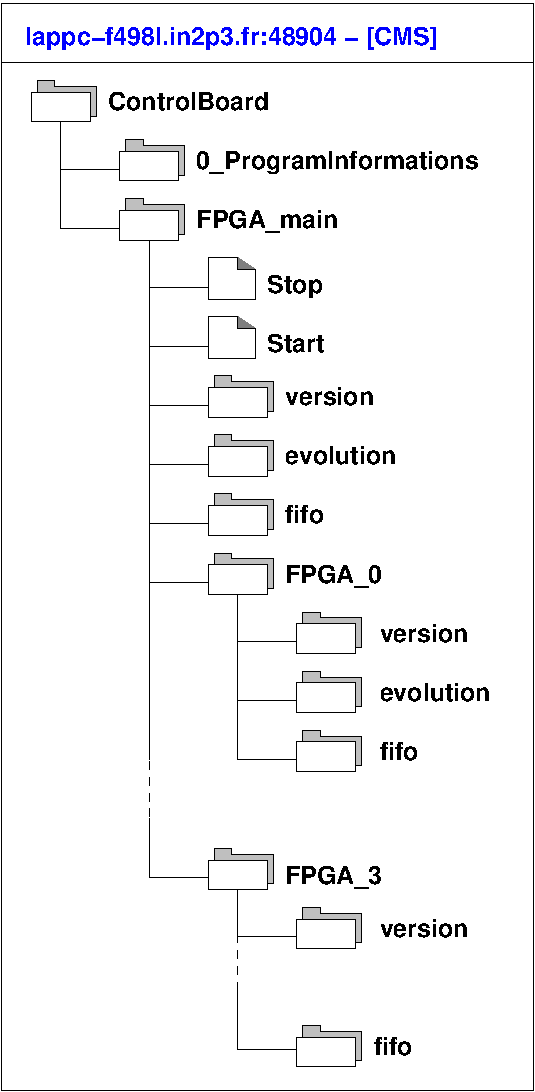
\includegraphics[width=5cm]{appendix/images/MOS_device_example_1.pdf}
\end{center}
\caption{Example of a  device managed through a MOS  server.  The root
  device is named \texttt{ControlBoard}.  First level daughter devices
  are  \texttt{0\_ProgramInformations} and  \texttt{FPGA\_main}.  Here
  the          MOS/OPCUA          server          is          labelled
  \texttt{CMS}.}\label{fig:an:mos_dev_1}
\end{figure}

% TODO


\subsection{Integration of a new device in the Vire environment}

The Vire  API also implements a  mechanism to describe a  hierarchy of
devices.  This  mechanism is independant  of the  one used in  the MOS
system but can  be easily made compatible with it.   This means that a
MOS  hierarchy  of devices  can  be  represented  in Vire.   The  Vire
hierarchy of  devices can  be considered as  some kind  of filesystem,
each device  being a folder with  its unique path, as  shown on figure
\ref{fig:an:mos_dev_2}.   The \emph{methods}  associated to  a devices
(or a datapoint) can be considered as plain executable files stored in
the  device's folder  : they  constitute the  set of  \emph{resources}
associated to the device.


\begin{figure}[h]
\begin{center}
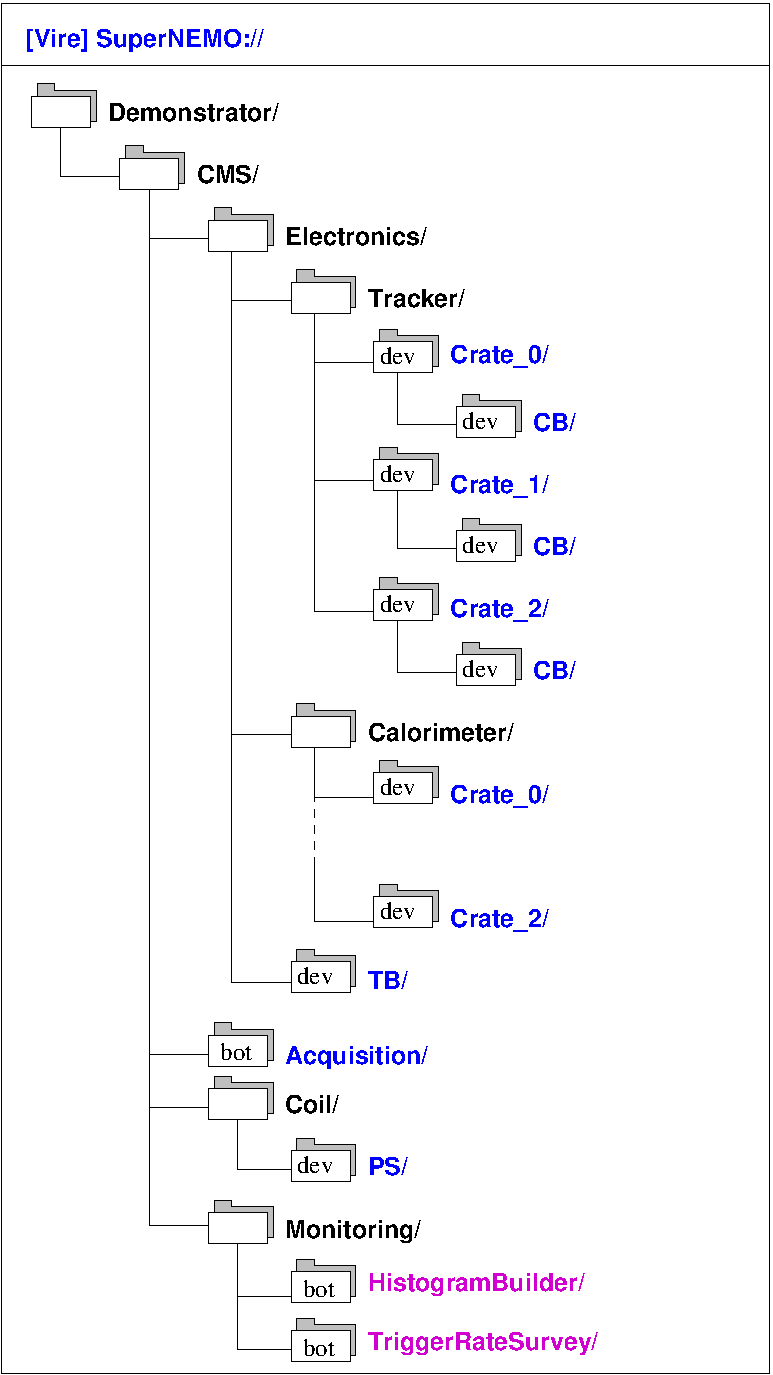
\includegraphics[width=5cm]{appendix/images/MOS_device_example_2.pdf}
\end{center}
\caption{Example of a hierarchy of  devices described by the Vire API.
  The root device is named  \texttt{SuperNEMO:}.  The top level (root)
  device  is  named  \texttt{Demonstrator}.  The  devices  colored  in
  \textcolor{blue}{blue}  are managed  through MOS/OPCUA.  The devices
  colored in \textcolor{magenta}{magenta} are directly embedded in the
  Vire server.  Devices with the \texttt{dev} tag are typical hardware
  device.  Devices  with the  \texttt{bot}  tag  are typical  software
  devices.   The  devices  colored in  \textbf{black}  are  structural
  pseudo-devices used to organize and  present a comprehensive view of
  the hierarchy. }\label{fig:an:mos_dev_2}
\end{figure}

The organisation of this hierarchy of devices is arbitrary and defined
by the designer of the  \emph{Control and Monitoring System}.  What is
important  to  understand  is  that  some  of  these  devices  can  be
associated  to  \emph{hardware  devices}  (a  power  supply  crate,  a
temperature probe\dots) and others  can be \emph{pseudo-devices}, i.e.
pure   software  object   (a   monitoring  robot,   a  file   transfer
daemon\dots).

In the context of the coupling of  the Vire server and the CMS server,
we are  in the event that  some devices are managed  by some MOS/OPCUA
servers and others are managed  in the Vire server itself.  Typically,
\emph{hardware devices}  are systematically managed through  the OPCUA
technology.  Vire has a mechanism to integrate such devices in its own
hierarchy.  This mechanism can  be considered like the \emph{mounting}
of   a   remote   filesystem   from  a   local   filesystem.    Figure
\ref{fig:an:mos_dev_0} illustrates  the case of many  hardware devices
-- managed by MOS -- that are integrated in the Vire system.  From the
Vire point of  view, the user does not see  the implementation details
for such  devices. He  does not  know the identity  of the  MOS server
hosting the device. He does not even know if the device is hosted by a
MOS server.  Devices are simply visible through the standard hierarchy
published by Vire with its  own device naming scheme, regardless their
true location.



\begin{figure}[h]
\begin{center}
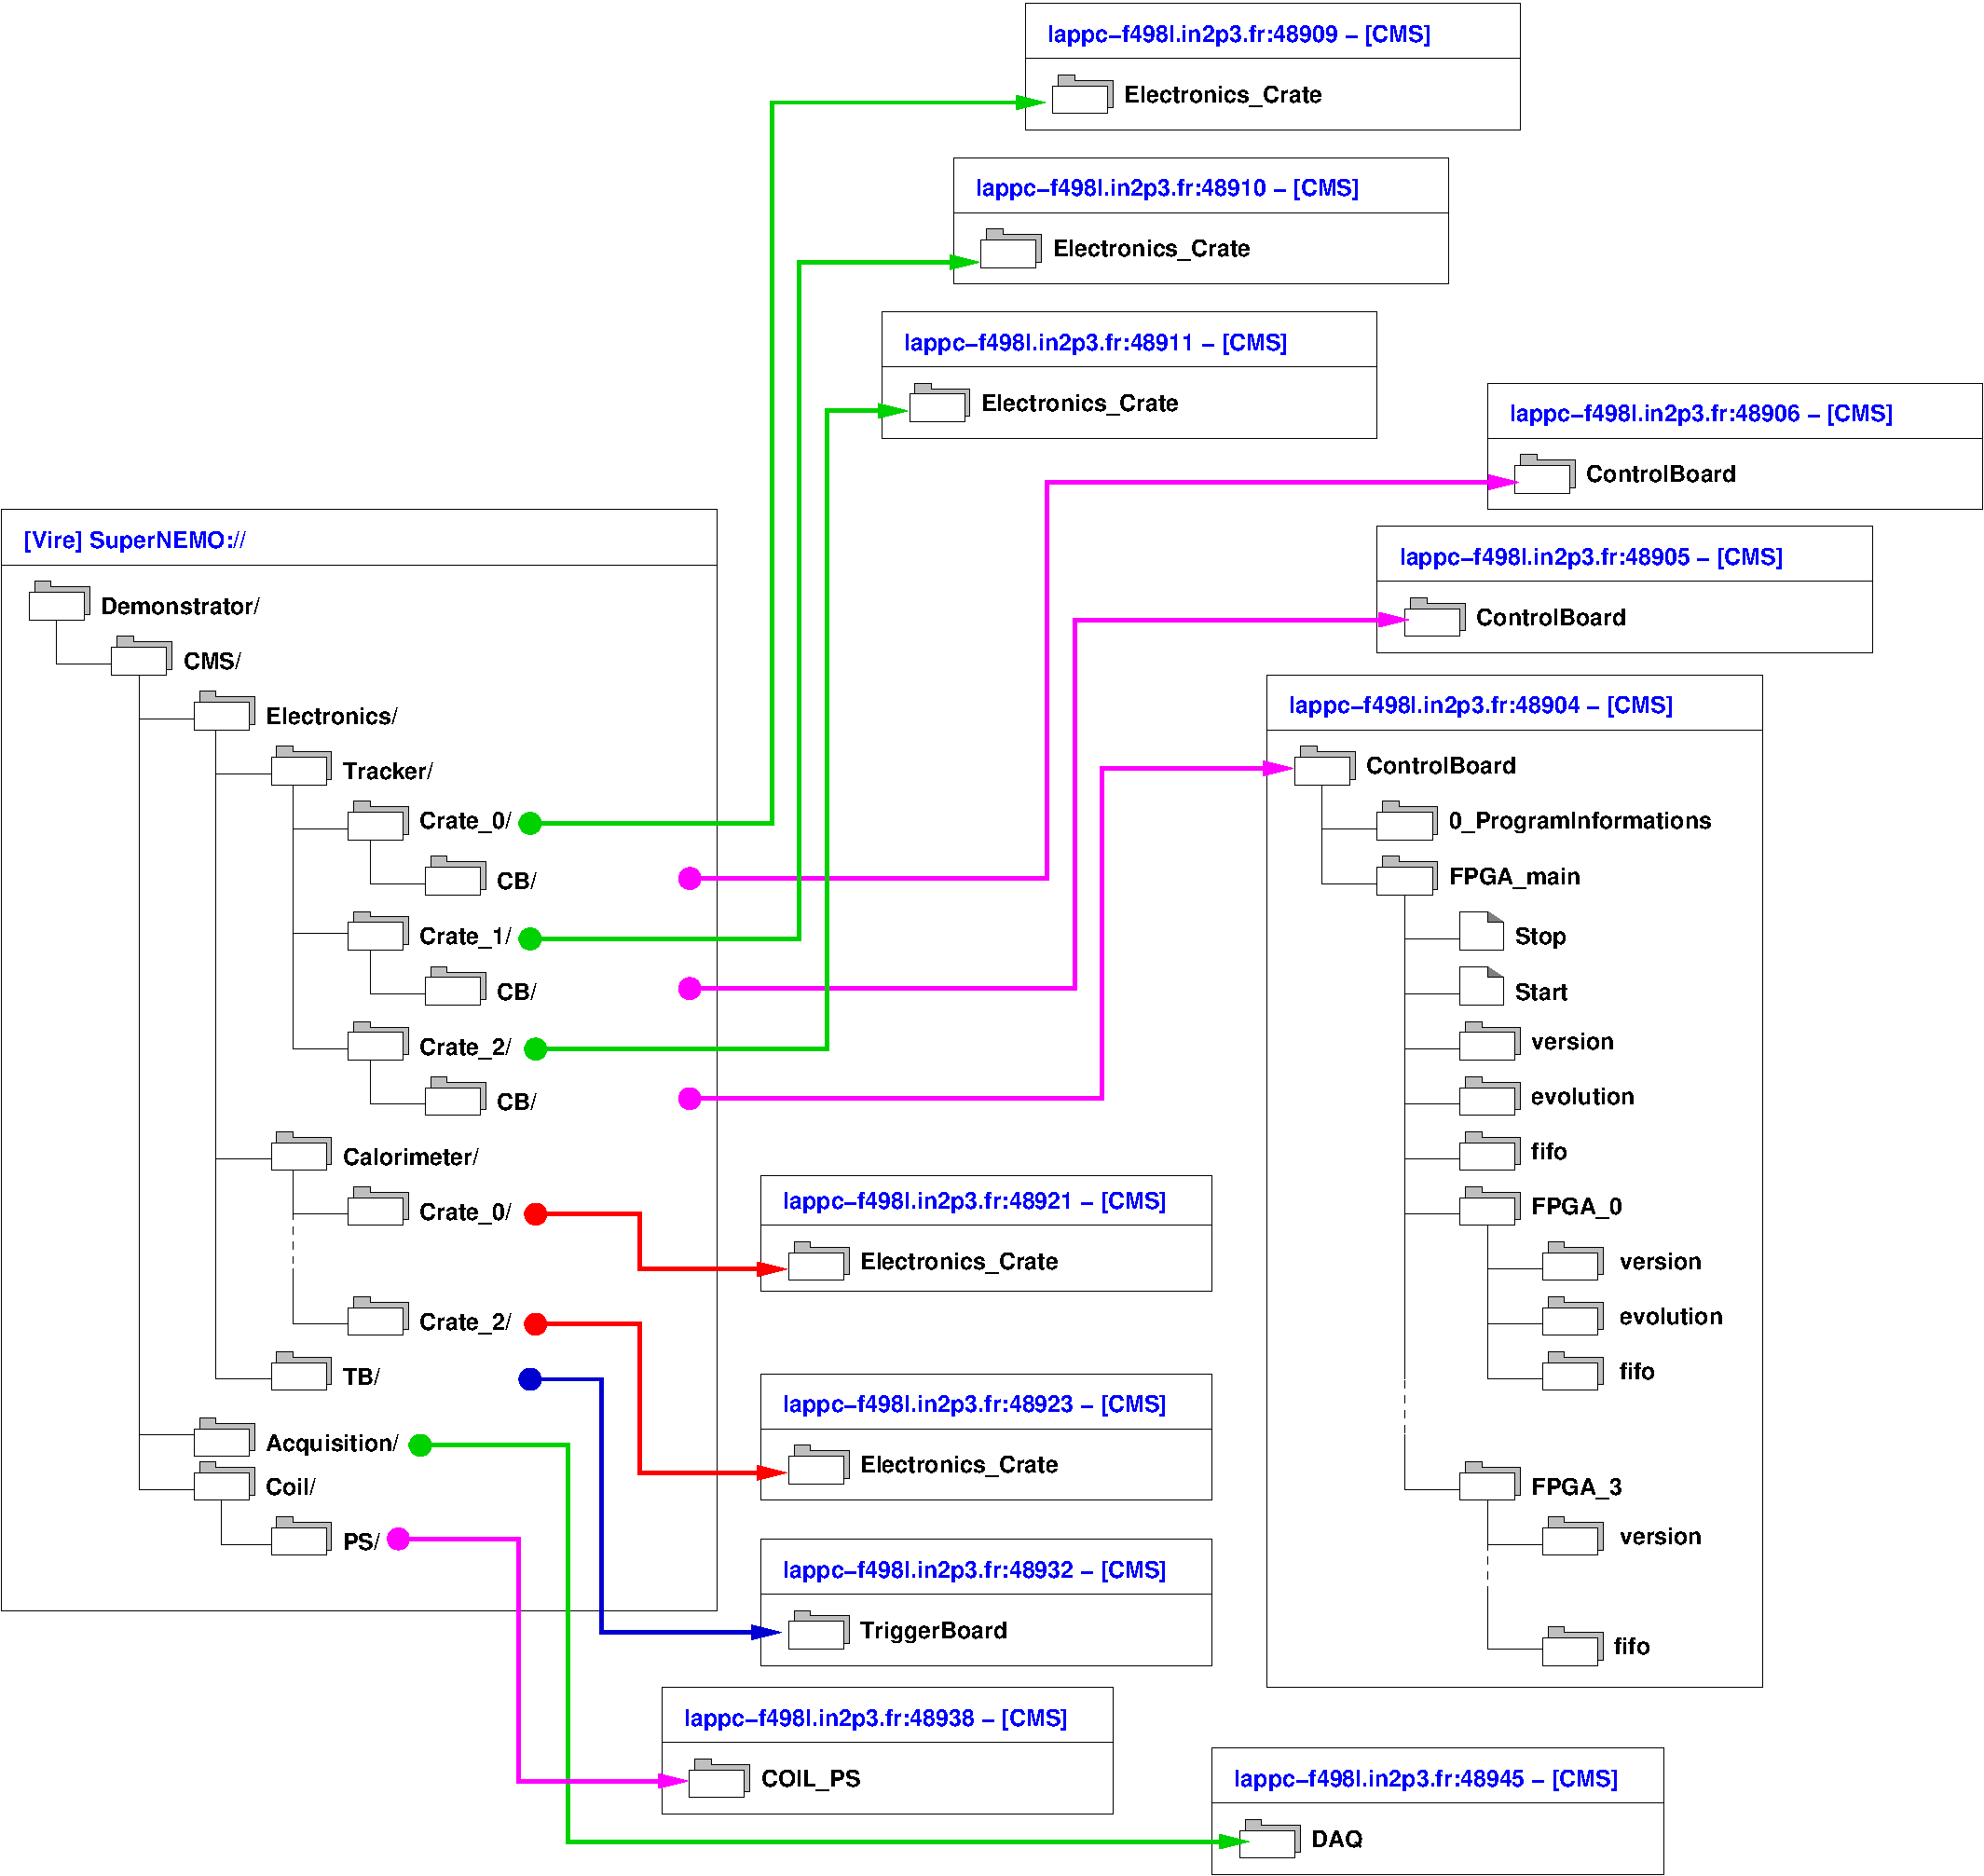
\includegraphics[width=\linewidth]{appendix/images/MOS_device_example_0.pdf}
\end{center}
\caption{The  mounting of  many  MOS device  hierarchies  in the  Vire
  device hierarchy.  Each OPCUA server  runs a simple  hardware device
  that is \emph{mounted} from a specific node with its own path.
%% of  devices described by the Vire API.
%%   The root device is named  \texttt{SuperNEMO:}.  The top level (root)
%%   device is  named \texttt{Demonstrator}. The devices  colored in blue
%%   are managed  through MOS/OPCUA. The  devices colored in  magenta are
%%   directly embedded in the Vire server.  Devices with the \texttt{dev}
%%   tag are typical  hardware device. Devices with  the \texttt{bot} tag
%%   are typical software devices.
}\label{fig:an:mos_dev_0}
\end{figure}




\subsection{Example}

Using  the examples  displayed  in  figure \ref{fig:an:mos_dev_0},  we
consider  in detail  the way  one specific  device managed  by MOS  is
mounted   in  the   Vire   hierarchy.  Figure   \ref{fig:an:mos_dev_3}
illustrates the mounting of a MOS device in Vire.

Here the Vire  server publishes the path of a  device representing the
control board  of the third  electronic crate  for the tracker  of the
SuperNEMO demonstrator module.  The full Vire path of this device is:

\textcolor{blue}{\texttt{SuperNEMO://Demonstrator/CMS/Electronics/Tracker/Crate\_2/CB}}

This is  the only Vire identifier  recognized by user to  address this
device.

On    the   figure,    one    can   see    that    the   MOS    server
\texttt{lappc−f498l.in2p3.fr} (port 48904) hosts a simple device which
is locally named \texttt{ControlBoard}.

When  mounting   this  device  in   the  Vire  hierarchy,   the  local
\texttt{[CMS]}  namespace and  \texttt{ControlBoard} device  names are
hidden and replaced by the Vire device path.  All daughter devices and
datapoints of  the \texttt{CMS/ControlBoard} device are  integrated as
daughters        of        the         Vire        device        named\\
\texttt{SuperNEMO://Demonstrator/CMS/Electronics/Tracker/Crate\_2/CB}.


For example, the \texttt{FPGA\_main} daughter device is now associated
to the following Vire path:

\textcolor{blue}{\texttt{SuperNEMO://Demonstrator/CMS/Electronics/Tracker/Crate\_2/CB/FPGA\_main/}}

and  its  \texttt{Stop} method  is  automatically  addressed with  the
following \emph{leaf} path:

\textcolor{blue}{\texttt{SuperNEMO://Demonstrator/CMS/Electronics/Tracker/Crate\_2/CB/FPGA\_main/Stop}}


\begin{figure}[h]
\begin{center}
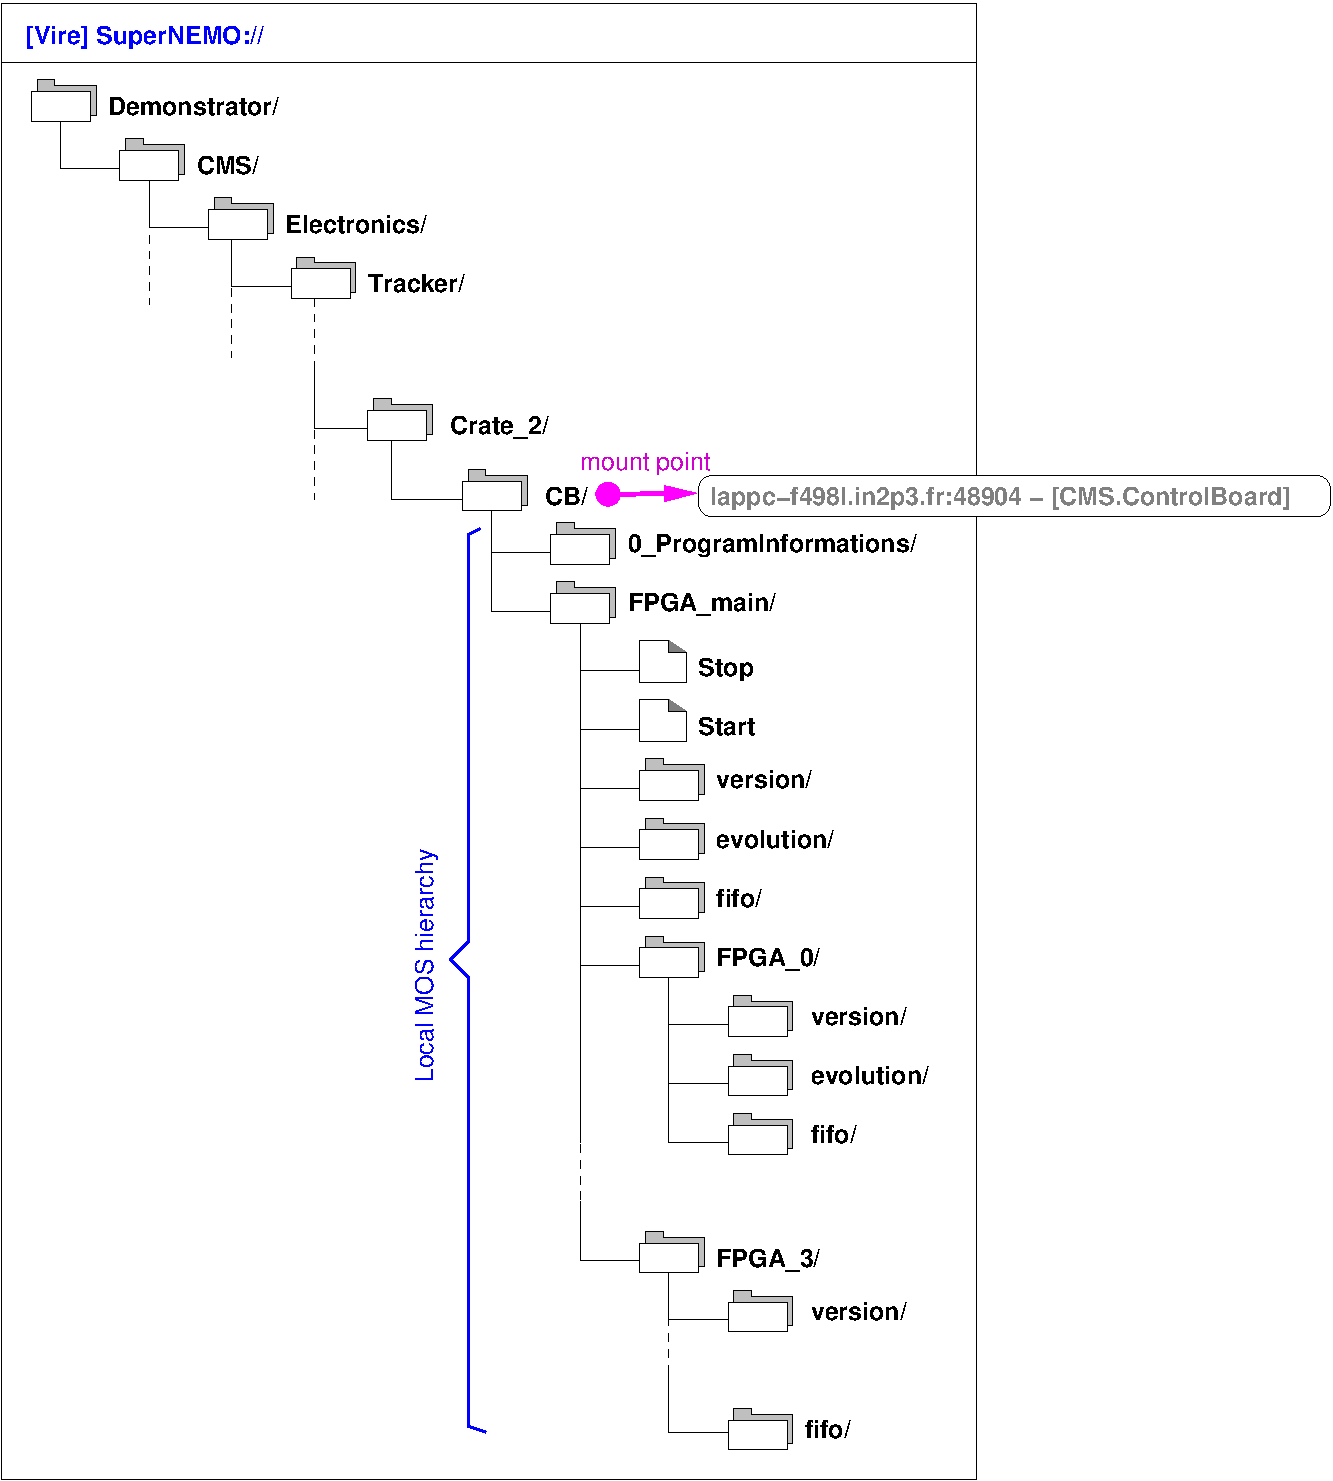
\includegraphics[width=0.8\linewidth]{appendix/images/MOS_device_example_3.pdf}
\end{center}
\caption{The  mounting of  one  MOS device and its local hierarchy  in the  Vire
  device hierarchy.}\label{fig:an:mos_dev_3}
\end{figure}



\subsection{Vire/MOS mapping}

As it can be  seen in the above example, the integration  of a new MOS
device in the Vire system is  achieved through soem kind of filesystem
mounting operation.   Particularly, it is  shown that the MOS  name of
the   mounted  root   device  is   replaced  by   an  arbitrary   Vire
path. However, all daughter  nodes (devices, datapoints) attached from
this root  node have their  relative MOS  names preserved in  the Vire
naming scheme.

Any  resource  (method)  associated  to any  of  such  daughter  nodes
inherits this relative naming scheme.

As Vire applications  describe resources through their  Vire paths, it
is thus needed to build an explicit map that associates resource paths
to MOS address  and name. The CMS  server will be able  to resolve the
MOS server/port and  embedded device associated to  the resource path.

The goal of the \texttt{devices\_launch.conf} file is not only to tell
the CMS server what MOS server should  be loaded and ran at start, but
also  to describe  the  \emph{mounting point/names}  used  by Vire  to
access the resources associated to MOS devices.  From the informations
stored in the  file, an explicit associative array must  be built when
the Vire server connect to the CMS server.  It will play the role of a
resource path resolver  when requests about resources will  be sent by
Vire applications.  This associative array  must be locked  during the
Vire/CMS connection.



%\subsubsection{Preparation of XML device models}

%% \noindent\underline{Pre-condition:}
%% The device is working and validated through the MOS/OPCUA server

%% \begin{enumerate}

%% \item Produce XML décrivant le modèle du device enrichi
%%   des metadata
%% Rédaction du fichier XML décrivant le modèle du device

%% \item Génération des fichiers model du type de device pour Vire

%% \item Génération des fichiers instances resolv.conf

%% \end{enumerate}


\vfill
\pagebreak
\clearpage

% end


\section{Vire messages}\label{app:vire_messages}

Within Vire  and between Vire  components and external  components, we
use  a communication  system  based on  Vire  messages.  This  section
describes the structure of such messages.

\subsection{General structure of a message}

Each message consists in two parts (figure \ref{fig-vire-message-message-cpp}):
\begin{itemize}

\item  the  \emph{header}  is   dedicated  to  generic  and  typicalle
  mandatory  informations  which  document   the  message  itself  and
  arbitrary high-level metadata.

\item  the \emph{body}  of the  message  contains the  real data: the payload.
  The structure of the message body depends on some convention. Vire uses
  its own convention to embed the payload data.

\end{itemize}

\begin{figure}[h]
\vskip 10pt
\small
\begin{Verbatim}[frame=single,xleftmargin=0.cm,label=\fbox{C++}]
struct vire::message::message {
  message_header header; // Header of the message
  message_body   body;   // Body of the message
};
\end{Verbatim}
\normalsize
\caption{The structure of a Vire message object (C++  class:
  \texttt{"vire::message::message"})}\label{fig-vire-message-message-cpp}
\end{figure}

\subsection{The message header}

The header contains (figure \ref{fig-vire-message-message_header-cpp}):
\begin{itemize}

  \item The mandatory \texttt{message\_id}  attribute is an identifier
    of the  message which  document the emitter  and a  unique message
    number.   Each emitter  is  responsible of  the  numbering of  the
    messages it  emits, typically using an  incremental technique. The
    message  number is  a positive  integer, starting  from 0  (figure
    \ref{fig-vire-message-message_identifier-cpp}).

  \item  The \texttt{timestamp}  attribute  encodes the  approximative
    time point when the message was  created. It contains the date and
    the time, using at least microsecond resolution.

    Typically,  with  JSON  encoding  system, it  is  expected  to  be
    formatted as a character string, using the following ISO format:

    \begin{center}
      \texttt{yyyymmddThhmmss.uuuuuu}
    \end{center}

    \noindent where:

    \vskip -10pt
    \begin{itemize}
    \item[\texttt{yyyymmdd} :] encodes year/month/day,
    \item[\texttt{hhmmssd} :] encodes hour/minute/second,
    \item[\texttt{uuuuuu} :] encodes microseconds.
    \end{itemize}

  \item   In   the   case    of   a   \emph{response}   message,   the
    \texttt{in\_reply\_to} attribute is set to identify the associated
    request message.

  \item  The \texttt{asynchronous}  boolean  attribute is  set if  the
    message processing  is explicitely requested  by the source  to be
    asynchronous (non-blocking).  In  RPC transactions, where requests
    are transmitted from one point to  the other, its default value is
    \emph{false}.   It  is possible  to  force  a RPC  transaction  in
    asynchronous mode.   This use  case is documented  elsewhere.  For
    event messaging, this flag is conventionally set to \emph{true}.

  \item  The  \texttt{body\_layout\_id}  attribute  is  the  mandatory
    identifier   of   the   layout   of  the   message   body   (class
    \texttt{"vire::utility::model\_identifier"}).  The  default layout
    for     message     body     inside    the     Vire     API     is
    \texttt{"vire::message::body\_format::typed\_payload"}, with version
    \texttt{"1.0"}                                             (figure
    \ref{fig-vire-utility-model_identifier-cpp}).

\end{itemize}


\begin{figure}[h]
\vskip 10pt
\small
\begin{Verbatim}[frame=single,xleftmargin=0.cm,label=\fbox{C++}]
struct vire::message::message_header {
  message_identifier message_id;     // Message identifier from the emitter.
  std::string        timestamp;      // Timestamp.
  message_identifier in_reply_to;    // Message identifier of the associated
                                     // request message (optional).
  bool               asynchronous,   // Asynchronous flag.
  vire::utility::model_identifier     body_layout_id; // Body layout identifier.
  std::map<std::string, std::string>  metadata;       // Key/value metadata dictionary.
};
\end{Verbatim}
\normalsize
\caption{The  structure  of  a   message  header  object  (C++  class:
  \texttt{"vire::message::message\_header"}).}\label{fig-vire-message-message_header-cpp}
\end{figure}

\begin{figure}[h]
\vskip 10pt
\small
\begin{Verbatim}[frame=single,xleftmargin=0.cm,label=\fbox{C++}]
struct vire::message::message_identifier {
  std::string emitter; // Name identifying the emitter of the message.
  int32_t     number;  // Number identifying the message in the emitter's
                       // message numbering scheme.
};
\end{Verbatim}
\normalsize
\caption{The      structure      of     a      message      identifier
  (C++  class:  \texttt{"vire::message::message\_identifier"}).}
\label{fig-vire-message-message_identifier-cpp}
\end{figure}

\begin{figure}[h]
\vskip 10pt
\small
\begin{Verbatim}[frame=single,xleftmargin=0.cm,label=\fbox{C++}]
struct vire::utility::model_identifier {
  std::string name;    // Name identifying the format of the message.
  std::string version; // String identifying the version of the format.
};
\end{Verbatim}
\normalsize
\caption{The structure of a model identifier (C++  class:  \texttt{"vire::utility::model\_identifier"}.}\label{fig-vire-utility-model_identifier-cpp}
\end{figure}




\begin{figure}[h]
\vskip 10pt
\small
\begin{Verbatim}[frame=single,xleftmargin=0.cm,label=\fbox{JSON}]
{
   "header" : {
      "message_id" : {
         "emitter" : "vire.server",
         "number" : 42
      },
      "timestamp" : "20160930T141408.413443",
      "in_reply_to" : {
         "initialized" : true,
         "value" : {
            "emitter" : "vire.client.0",
            "number" : 23
         }
      },
      "asynchronous" : false,
      "body_layout_id" : {
         "name" : "vire::message::body_format::typed_payload",
         "version" : {
            "initialized" : true,
            "value" : "1.0"
         }
      },
      "metadata" : [
         {
            "key" : "key1",
            "value" : "foo"
         },
         {
            "key" : "key2",
            "value" : "42"
         },
         {
            "key" : "key3",
            "value" : "3.1415899999999999"
         },
         {
            "key" : "key4",
            "value" : "true"
         }
      ]
   }
  "body" : {
      ...
   }
}
\end{Verbatim}
\normalsize
\caption{Example of  a   message  header  object in JSON format.}
\label{fig-vire-message-message_header-json}
\end{figure}

\vfill
\clearpage
\pagebreak

\subsection{The message body}

The    default    message   body    layout    in    Vire   is    named
\texttt{"vire::message::body\_format::typed\_payload"}        (version
\texttt{"1.0"}).   Each  message used  within  the  Vire framework  is
supposed to use this layout.  The general idea is that the body of the
message embeded the  \emph{payload object} that has  to be transmitted
between  two components  of  the system.   \emph{Payload objects}  are
classified in one of the three following categories:

\begin{enumerate}

\item \emph{Request}:  describes a request submitted  by one component
  to another component (generally during a synchronous RPC transaction).

\item  \emph{Response}: describes  the  response to  a former  request
  (generally during a synchronous RPC transaction).

\item \emph{Event}: describes an  arbitrary information record (alarm,
  exception, signal\dots) which is transmitted asynchronously.

\end{enumerate}

Vire implements the following class hierarchy:

\begin{center}
\begin{tikzpicture}
  \node (payload)  at (0,2)  [draw] {\texttt{vire::utility::base\_payload}};
  \node (request)  at (-4,0) [draw] {\texttt{vire::utility::base\_request}};
  \node (response) at (2,0)  [draw] {\texttt{vire::utility::base\_response}};
  \node (event)    at (8,0)  [draw] {\texttt{vire::utility::base\_event}};

  %\draw[style=help lines] (-3,-1) grid (10,4);
  \draw (node cs:name=response,anchor=north) |- (0,1);
  \draw (node cs:name=event,anchor=north)    |- (0,1);
  \draw[->] (node cs:name=request,anchor=north)
  |- (0,1) -| (node cs:name=payload,anchor=south);
\end{tikzpicture}
\end{center}

The requirements for the transmitted object are the following:

\begin{itemize}

\item The  type of the object  must be conventionally associated  to a
  unique     \emph{model      identifier}     object      (see     the
  \texttt{"vire::utility::model\_identifier"} class)  which contains a
  unique   name   (\textit{string    identifier})   and   possibly   a
  \textit{version identifier}.  Each software  component that may send
  or  receive the  object  should agree  on  this type  identification
  scheme.   This   enable  the  use  of   object  factories,  whatever
  programming  langage  is used  on  both  side of  the  communication
  system.

\item  For each  software component,  the object  type must  have some
  dedicated  encoding/decoding  functions  available  (again  whatever
  programming language is used). For example the Vire API supports the
  following encoding formats:

  \begin{itemize}

  \item JSON (MIME  encoding type: \texttt{"application/x-json"}), which
    is supportable by many languages,

  \item  Protobuf  (Google  Protocol   Buffers,  MIME  encoding  type:
    \texttt{"application/x-protobuf"}), which is also widely supported,

  \item   Boost/serialisation   (XML,    text   or   binary   archives
    \texttt{"application/x-boost-serialization-xml"},
    \texttt{"application/x-boost-serialization-text"},
    \texttt{"application/x-boost-serialization-binary"}),    which    in
    principle is supported by C++ only.

  \end{itemize}

  The Protobuf  encoding format will be  used to serialize/deserialize
  the  Vire  messages transported  between  the  Vire server  and  the
  CMS/LAPP server.

\end{itemize}

Vire uses a dedicated layout to represent the body of any message with
its embedded payload object. With this technique, the structure of the
body          contains         two          attributes         (figure
\ref{fig-app-vire-message-message_body-cpp}):

\begin{enumerate}

\item The \texttt{payload\_type\_id} specifies the type of the payload
  object   (figure   \ref{fig-app-vire-utility-model_identifier-cpp}).
  This unique name  is conventionaly fixed for a  given application. A
  version tag allows to support possible evolution of the object type.

\item The  \texttt{payload} is a  handle to  a payload object  of type
  request, response or event.

  %% \begin{itemize}
  %% \item Within  the producer  component of  the message,  the encoding
  %%   function associated to the object  type is responsible to generate
  %%   the JSON stream for the object and store it in the buffer.

  %% \item Within  the consumer  component of  the message,  the decoding
  %%   function associated to the object type is responsible to parse the
  %%   JSON stream stored in the buffer and restore the object in memory.

  %% \end{itemize}

  It is expected  that, on both sides of the  connection, the software
  components can  access dedicated  software plugins which  ensure the
  support  of  various   \emph{payload  object  types}  conventionnaly
  associated  with  their  \emph{payload type  identifiers}  and  also
  providing JSON and/or Protobuf encoding/decoding functionalities.

  %% The   system  allows  to  support
  %% modification  in the  structure of  the objects  thanks to  version
  %% tagging.

\end{enumerate}

\begin{figure}[h]
\vskip 10pt
\small
\begin{Verbatim}[frame=single,xleftmargin=0.cm,label=\fbox{C++}]
struct message_body {
  vire::utility::model_identifier     payload_type_id; // Object type identifier.
  const vire::utility::base_payload * payload;         // Handle to a payload object.
};
\end{Verbatim}
\normalsize
\caption{The structure of a message body object (C++).}
\label{fig-app-vire-message-message_body-cpp}
\end{figure}

\begin{figure}[h]
\vskip 10pt
\small
\begin{Verbatim}[frame=single,xleftmargin=0.cm,label=\fbox{JSON}]
{
  "header" : {
    ...
  },
  "body" : {
    "payload_type_id" : {
      "name" : "vire::message::testing::error_event",
      "version" : {
        "initialized" : false
      }
    },
    "payload" : {
      "timestamp" : "20160930T141743.759085"
      "err" : {
        "code" : 3,
        "message" : "A basic error"
      },
    }
  }
}
\end{Verbatim}
\normalsize
\caption{Example of  a   message  body  object in JSON format.}
\label{fig-vire-message-message_body-json}
\end{figure}

\vfill
\clearpage
\pagebreak

% end

%\input{appendix/app_json_fmt.tex}

\section{The \emph{Protocol Buffers} format}\label{app:protobuf_fmt}

\subsection{Introduction}

The  Google  Protocol Buffers  (\emph{protobuf})  library  is used  to
represent the objects that are exchanged between the Vire clients, the
Vire server and the CMS server.  The  version 3 of the format is used,
implying   at   least   version   3.0.0  (September   2016)   of   the
\emph{protobuf} library.

Each  data   structure  of  interest   can  be  described   through  a
\texttt{.proto}  file  from  which  stub files  can  be  automatically
generated  with the  \texttt{protoc} compiler.  For Vire  and its  CMS
interface, the C++ and Java programming languages will be used.


A  collection of  \texttt{.proto}  files are  provided  with the  Vire
library to represent all kind  of data structures transferable between
networked agents  (Vire server,  Vire clients, CMS/LAPP  server).  The
objects of  the highest level  are named \emph{payload  objects} (like
\emph{request},  \emph{response} and  \emph{event} objects).   They
are composed of attributes of more basic data structures.

\subsection{Example}

The following  class diagram  illustrates two data  structures defined
within the Vire library with an inheritance relationship between them.

\begin{center}
  \begin{tikzpicture}
    \node (base)     at (0,1.5)  [draw] {\texttt{vire::utility::base\_error}};
    \node (setup)    at (0,0)  [draw] {\texttt{vire::utility::invalid\_setup\_id\_error}};

    \draw[->]   (node cs:name=setup,anchor=north) |- (0,1);
    |- (0,1) -| (node cs:name=base,anchor=south);
  \end{tikzpicture}
\end{center}

The \texttt{vire::utility::base\_error}  is the  parent class  for all
\emph{error}  objects.   It  contains   two  attributes:   an  integer
\emph{error code}  and a  character string describing  the \emph{error
  message}.

The   \texttt{vire::utility::invalid\_setup\_id\_error}  class   is  a
specialized error class  which represents explicitely an  error due to
an identification  failure of  the experimental setup.   It implements
additional mutually exclusive attributes: the \emph{unrecognized name}
of the setup or the \emph{unrecognized version} of the setup.

This   example  illustrates   the  protobuf   representation  of   the
\texttt{vire::utility::base\_error}  in the  Vire  library, using  the
\texttt{"vire/utility/BaseError.proto"} file:

\small
\begin{Verbatim}[frame=single,xleftmargin=0.cm,label=\fbox{protobuf}]
  syntax = "proto3";
  package vire.utility; // Namespace

  message BaseError {

    // reserved 1; // Reserved for _base message

    // Attributes:
    int32  code           = 100; // The error code
    string message_format = 101; // The error description message

  }
\end{Verbatim}
\normalsize

\vfill
\clearpage
\pagebreak

\subsection{Vire protobuf conventions}

Vire uses the following conventions:

\begin{enumerate}

\item
  The member index  \texttt{1} is reserved to represent the  link of a
  class to its main base/parent class (if any).  It is not used if the
  data structure does not inherit any data structure.
  If a data structure naturally inherits another one, it is thus possible
  to  represent the  inheritance  relationship as  illustrated with  the
  \texttt{"vire/utility/InvalidSetupIdError.proto"}      file      which
  represents the \texttt{vire::utility::invalid\_setup\_id\_error} class
  in the Vire library:

  \small
  \begin{Verbatim}[frame=single,xleftmargin=0.cm,label=\fbox{protobuf}]
    syntax = "proto3";
    package vire.utility; // Namespace

    import "vire/utility/BaseError.proto"; // Dependency

    message InvalidSetupIdError {

      BaseError _base = 1; // The base class

      // Additional attributes:
      oneof detail { // Mutual exclusion
        string invalid_setup_name    = 100; // The failed setup name
        string invalid_setup_version = 101; // The failed setup version
      }

    }
  \end{Verbatim}
  \normalsize

\item The  \texttt{\_base} member  is conventionally  used to  represent the
  inheritance   relationship    from   a   data   structure    of   type
  \texttt{"vire.utility.BaseError"}.

\item Member indexes from \texttt{2}  to \texttt{99} are also reserved
  for possible future usage (multiple inheritance, metadata\dots).

\item
  The first member of the data structure must start at index \texttt{100}.

\end{enumerate}

\vfill
\clearpage
\pagebreak

% end


\section{Vire payload objects}\label{app:payload}

\subsection{Introduction}

As  mentioned in  appendix \ref{app:protobuf_fmt},  Vire messages  are
wrappers for \emph{payload objects}.  Each  type of payload object can
be represented  through the \emph{protobuf} mechanism.   The following
class hierarchy shows the base architecture used to define new payload
objects.

\begin{center}
\begin{tikzpicture}
  \node (payload)  at (0,2)   [draw] {\texttt{vire::utility::base\_payload}};
  \node (request)  at (-4,0)  [draw] {\texttt{vire::utility::base\_request}};
  \node (response) at (2,0)   [draw] {\texttt{vire::utility::base\_response}};
  \node (event)    at (8,0)   [draw] {\texttt{vire::utility::base\_event}};
  \node (my)       at (-4,-2) [draw] {\texttt{my\_request}};
  \node (your)     at (2,-2)  [draw] {\texttt{your\_response}};
  \node (its)    at (8,-2)    [draw] {\texttt{its\_alarm}};

  %\draw[style=help lines] (-6,-2) grid (10,2);
  \draw (node cs:name=response,anchor=north) |- (0,1);
  \draw (node cs:name=event,anchor=north)    |- (0,1);
  \draw[->] (node cs:name=request,anchor=north)
  |- (0,1) -| (node cs:name=payload,anchor=south);
  \draw[->] (node cs:name=my,anchor=north)
  |- (-4,-1) -| (node cs:name=request,anchor=south);
  \draw[->] (node cs:name=your,anchor=north)
  |- (2,-1) -| (node cs:name=response,anchor=south);
  \draw[->] (node cs:name=its,anchor=north)
  |- (8,-1) -| (node cs:name=event,anchor=south);
\end{tikzpicture}
\end{center}


\begin{center}
\vskip 10pt
\small
\begin{tabular}{|l|l|l|}
  \hline
  \textbf{Vire C++ class} & \textbf{protobuf message type} & \textbf{protobuf definition file} \\
  \hline
  \hline
  \multicolumn{3}{|c|}{\emph{general types}} \\
  \hline
  boost::posix\_time::ptime & google.protobuf.Timestamp & google/protobuf/timestamp.proto \\
  \hline
  \hline
  \multicolumn{3}{|c|}{\emph{identifier types}} \\
  \hline
  vire::utility::base\_identifier & vire.utility.Baseidentifier & vire/utility/Baseidentifier.proto \\
  \hline
  vire::utility::instance\_identifier & vire.utility.InstanceIdentifier & vire/utility/InstanceIdentifier.proto \\
  \hline
  vire::utility::model\_identifier & vire.utility.ModelIdentifier & vire/utility/ModelIdentifier.proto \\
  \hline
  \hline
  \multicolumn{3}{|c|}{\emph{error types}} \\
  \hline
  vire::utility::base\_error & vire.utility.BaseError & vire/utility/BaseError.proto \\
  \hline
  vire::utility::invalid\_context\_error & vire.utility.InvalidContextError & vire/utility/InvalidContextError.proto \\
  \hline
  vire::utility::invalid\_setup\_id\_error & vire.utility.InvalidSetupIdError & vire/utility/InvalidSetupIdError.proto \\
  \hline
  \hline
  \multicolumn{3}{|c|}{\emph{payload types}} \\
  \hline
  vire::utility::base\_payload & vire.utility.BasePayload & vire/utility/BasePayload.proto \\
  \hline
  vire::utility::base\_request & vire.utility.BaseRequest & vire/utility/BaseRequest.proto \\
  \hline
  vire::utility::base\_response & vire.utility.BaseResponse & vire/utility/BaseResponse.proto \\
  \hline
  vire::utility::base\_event & vire.utility.BaseEvent & vire/utility/BaseEvent.proto \\
  \hline
  vire::utility::base\_alarm & vire.utility.BaseAlarm & vire/utility/BaseAlarm.proto \\
  \hline
  \hline
  \multicolumn{3}{|c|}{\emph{messenging types}} \\
  \hline
  vire::message::message\_identifier & vire.message.MessageIdentifier & vire/message/MessageIdentifier.proto \\
  \hline
  vire::message::msg\_header & vire.message.MsgHeader & vire/message/MsgHeader.proto \\
  \hline
  vire::message::msg\_body & vire.message.MsgBody & vire/message/MsgBody.proto \\
  \hline
  vire::message::message & vire.message.Message & vire/message/Message.proto \\
  \hline
\end{tabular}
\normalsize
\end{center}


\begin{center}
\vskip 10pt
\small
\begin{tabular}{|l|l|l|}
  \hline
  \multicolumn{3}{|c|}{\emph{Resource management related types}} \\
  \hline
  vire::cms::resource\_status\_record & vire.cms.ResourceStatusRecord & vire/cms/ResourceStatusRecord.proto \\
  \hline
  vire::cms::resource\_fetch\_status\_request & vire.cms.ResourceFetchStatusRequest & vire/cms/ResourceFetchStatusRequest.proto \\
  \hline
  vire::cms::resource\_fetch\_status\_success\_response & vire.cms.ResourceFetchStatusSuccessResponse & vire/cms/ResourceFetchStatusSuccessResponse.proto \\
  \hline
  vire::cms::resource\_fetch\_status\_failure\_response & vire.cms.ResourceFetchStatusFailureResponse & vire/cms/ResourceFetchStatusFailureResponse.proto \\
  \hline
  vire::cms::resource\_exec\_request & vire.cms.ResourceExecRequest & vire/cms/ResourceExecRequest.proto \\
  \hline
  vire::cms::resource\_exec\_success\_response & vire.cms.ResourceExecSuccessResponse & vire/cms/ResourceExecSuccessResponse.proto \\
  \hline
  vire::cms::resource\_exec\_failure\_response & vire.cms.ResourceExecFailureResponse & vire/cms/ResourceExecFailureResponse.proto \\
  \hline
  vire::cms::resource\_exec\_non\_blocking\_request & vire.cms.ResourceExecNonBlockingRequest & vire/cms/ResourceExecNonBlockingRequest.proto \\
  \hline
  vire::cms::resource\_exec\_non\_blocking\_ack\_response & vire.cms.ResourceExecNonBlockingAckResponse & vire/cms/ResourceExecNonBlockingAckResponse.proto \\
  \hline
  vire::cms::resource\_exec\_non\_blocking\_noack\_response & vire.cms.ResourceExecNonBlockingNoackResponse & vire/cms/ResourceExecNonBlockingNoackResponse.proto \\
  \hline
  vire::cms::resource\_exec\_non\_blocking\_success\_event & vire.cms.ResourceExecNonBlockingSuccessEvent & vire/cms/ResourceExecNonBlockingSuccessEvent.proto \\
  \hline
  vire::cms::resource\_exec\_non\_blocking\_failure\_event & vire.cms.ResourceExecNonBlockingFailureEvent & vire/cms/ResourceExecNonBlockingFailureEvent.proto \\
  \hline
  vire::cms::resource\_exec\_error & vire.cms.ResourceExecError & vire/cms/ResourceExecError.proto \\
  \hline
  vire::cms::invalid\_status\_error & vire.cms.ResourceExecError & vire/cms/ResourceExecError.proto \\
  \hline
  %% vire::cms::invalid\_credentials\_error & vire.cms.InvalidCredentialsError & vire/cms/InvalidCredentialsError.proto \\
  %% \hline
  %% vire::cms::invalid\_user\_error & vire.cms.InvalidUserError & vire/cms/InvalidUserError.proto \\
  %% \hline
  vire::cms::invalid\_resource\_error & vire.cms.InvalidUserError & vire/cms/InvalidUserError.proto \\
  \hline
  vire::cms::no\_pubsub\_resource\_error & vire.cms.NoPubsubResourceError & vire/cms/NoPubsubResourceError.proto \\
  \hline
  \hline
  \multicolumn{3}{|c|}{\emph{Resource pub/sub management types}} \\
  \hline
  vire::cms::resource\_pubsub\_subscribe\_request & vire.cms.ResourcePubsubSubscribeRequest & vire/cms/ResourcePubsubSubscribeRequest.proto \\
  \hline
  vire::cms::resource\_pubsub\_subscribe\_success\_response & vire.cms.ResourcePubsubSubscribeRSuccessResponse & vire/cms/ResourcePubsubSubscribeRSuccessResponse.proto \\
  \hline
  vire::cms::resource\_pubsub\_subscribe\_failure\_response & vire.cms.ResourcePubsubSubscribeRFailureResponse & vire/cms/ResourcePubsubSubscribeRSuccessResponse.proto \\
  \hline
  \hline
  \multicolumn{3}{|c|}{\emph{Vire/CMS server interface types}} \\
  \hline
  vire::cmsinterface::connection\_request & vire.cmsinterface.ConnectionRequest & vire/cmsinterface/ConnectionRequest.proto \\
  \hline
  vire::cmsinterface::connection\_success\_response & vire.cmsinterface.ConnectionSuccessResponse & vire/cmsinterface/ConnectionSuccessResponse.proto \\
  \hline
  vire::cmsinterface::connection\_failure\_response & vire.cmsinterface.ConnectionFailureResponse & vire/cmsinterface/ConnectionFailureResponse.proto \\
  \emph{embedded:} unknown\_resources\_error & .UnknownResourcesError &  \\
  \hline
  vire::cmsinterface::disconnection\_request & vire.cmsinterface.DisconnectionRequest & vire/cmsinterface/DisconnectionRequest.proto \\
  \hline
  vire::cmsinterface::disconnection\_success\_response & vire.cmsinterface.DisconnectionSuccessResponse & vire/cmsinterface/DisconnectionSuccessResponse.proto \\
  \hline
  %% \hline
  %% vire::cmsinterface::disconnection\_failure\_response & vire.cmsinterface.DisconnectionFailureResponse & vire/cmsinterface/DisconnectionFailureResponse.proto \\
\end{tabular}
\normalsize
\end{center}

\subsection{Basic data structures}

Any  payload object  (request, response  or event)  generally contains
some information records which are  specific to the functionalities of
the  payload  object they  belong.   These  records are  of  arbitrary
types. Of course they should be  translatable in terms of the protobuf
library.
%Of course they can be (de)serialized using JSON.
Some of these types are very  general and defined within the Vire core
API itself because they are reused by various payload objects not only
through  the Vire-CMS/LAPP  interface  but also  between  Vire clients  and
servers, independently  of the  CMS/LAPP server.  However,  the use  of the
Protocol Buffers interface makes possible  to publish the interface of
such data to the outside world, including the CMS/LAPP server in priority.

%% Other one are specific to the Vire/CMS interface and thus managed only
%% in the \texttt{Vire\_CMSInterface} API.
These  types  are considered  as  \emph{basic}.  Among them  we  find:
generic error  types, generic  identifier types,  timestamps, resource
status records\dots We propose to describe them in this section.

Once a sufficient collection of  basic data record types is available,
it  is possible  to describe  high  level payload  object types  which
aggregate attributes of such types.

Other record  types are specific to  some payload objects and  will be
never  used outside  the scope  of these  payload objects.   Such data
structures will be  explicitely declared with the  payload object they
belong to, likely as embedded types/classes.


\subsubsection{Errors}

Some  \emph{response} or  \emph{event} payload  objects may  contain a
specific  error  record  object.   A  \emph{failure  response}  or  an
\emph{exception  event}  object will  generally  embed  such an  error
record object.

Each  \emph{error record}  is represented  by an  instance of  a given
error type.   Each of  the error  types defined  in Vire  inherits the
\texttt{vire::utility::base\_error}      base       class      (figure
\ref{fig-app-payload-base_error})   which   contains   the   following
attributes:

\begin{itemize}

\item the error code: A non zero  integer which is set to 1 by default
  (indicating  a  generic  failure  case).   The  error  code  can  be
  conventionally  set to  any positive  integer value  to represent  a
  specific error case, depending on the context.

\item the error  message: an optional human  readable character string
  which documents the error as usefully as possible.

\end{itemize}

\begin{figure}[h]
\vskip 10pt
\small
\begin{Verbatim}[frame=single,xleftmargin=0.cm,label=\fbox{C++}]
struct vire::utility::base_error
{
  // Attributes:
  int         code;           // Error code (>0).
  std::string message_format; // Error message (optional).
};
\end{Verbatim}
\normalsize
\caption{The structure of a \texttt{"vire::utility::base\_error"} object
  (C++).}
\label{fig-app-payload-base_error}
\end{figure}


%% An example of JSON formatted basic error object is given in figure
%% \ref{fig-app-payload-base_error-1}.
%%
%% \begin{figure}[h]
%% \vskip 10pt
%% \small
%% \begin{Verbatim}[frame=single,xleftmargin=0.cm,label=\fbox{\texttt{JSON}}]
%% {
%%   "code" : "42",
%%   "message_format" : "Invalid AMQP server port=[2341]"
%% }
%% \end{Verbatim}
%% \normalsize
%% \caption{JSON  formatted  basic  error  object  (class
%%   \texttt{vire::utility::base\_error}.}
%% \label{fig-app-payload-base_error-1}
%% \end{figure}

Several type of generic errors are defined in Vire:


\begin{center}
\begin{tikzpicture}
  \node (base)     at (0,2)  [draw] {\texttt{vire::utility::base\_error}};
  \node (context)  at (-4,0) [draw] {\texttt{vire::utility::invalid\_context\_error}};
  \node (setup)    at (0,-1)  [draw] {\texttt{vire::utility::invalid\_setup\_id\_error}};
  \node (resource) at (4,0)  [draw] {\texttt{vire::cms::invalid\_resource\_error}};
  \node (user)     at (8,-1)  [draw] {\texttt{vire::cms::invalid\_user\_error}};

  \draw     (node cs:name=setup,anchor=north)    |- (0,1);
  \draw     (node cs:name=resource,anchor=north) |- (0,1);
  \draw     (node cs:name=user,anchor=north)     |- (0,1);
  \draw[->] (node cs:name=context,anchor=north)
  |- (0,1) -| (node cs:name=base,anchor=south);
\end{tikzpicture}
\end{center}

\noindent
Here are a few error object types defined in Vire.  Some types belongs
to the \texttt{utility} namespace, other  ones are in the \texttt{cms}
namespace:

\begin{itemize}

\item \texttt{"vire::utility::invalid\_context\_error"} : occurs typically when
  the general context of the execution of a given resource is not adapted.\\
  It is mapped to the \texttt{"vire.utility.InvalidContextError"} protobuf record.

\item \texttt{"vire::utility::invalid\_setup\_id\_error"} : occurs in case
  of an invalid identification of the experimental setup managed
  by the Vire or CMS server.\\
  It is mapped to the \texttt{"vire.utility.InvalidSetupIdError"} protobuf record.

\item \texttt{"vire::cms::invalid\_resource\_error"} : occurs in case
  of an invalid identification of a resource.\\
  It is mapped to the  \texttt{"vire.cms.InvalidResourceError"} protobuf record.

\item \texttt{"vire::cms::invalid\_status\_error"}: occurs when an attempt
  to access a resource that has not the proper status.\\
  It is mapped to the  \texttt{"vire.cms.InvalidStatusError"} protobuf record.

\item \texttt{"vire::cms::invalid\_user\_error"} : occurs in case
  of an invalid identification of an user.\\
  It is mapped to the  \texttt{"vire.cms.InvalidUserError"} protobuf record.

\item \texttt{"vire::cms::invalid\_credentials\_error"} : occurs in case
  of user authentication error.\\
  It is mapped to the  \texttt{"vire.cms.InvalidCredentialsError"} protobuf record.

\item \texttt{"vire::cms::resource\_exec\_error"} : occurs in case
  of error at the execution of a given resource.\\
  It is mapped to the  \texttt{"vire.cms.ResourceExecError"} protobuf record.

\end{itemize}



\subsubsection{Object and type identifiers}

Vire  uses  some dedicated  classes  to  represent the  identifier  of
various objects  (or \emph{instances})  as well  as various  types (or
\emph{models})  of components.  Vire  implements  the following  class
hierarchy:

\begin{center}
\begin{tikzpicture}
  \node (base)  at (0,2)  [draw] {\texttt{vire::utility::base\_identifier}};
  \node (instance)  at (-4,0) [draw] {\texttt{vire::utility::instance\_identifier}};
  \node (model) at (4,0)  [draw] {\texttt{vire::utility::model\_identifier}};

  \draw (node cs:name=model,anchor=north) |- (0,1);
\draw[->] (node cs:name=instance,anchor=north)
  |- (0,1) -| (node cs:name=base,anchor=south);
\end{tikzpicture}
\end{center}

The          \texttt{vire::utility::base\_identifier}          (figure
\ref{fig-app-payload-base_identifier}) class is  a pure abstract class
that cannot be instantiated. However  it contains a mandatory name and
an  optional  version description  which  are  used by  all  inherited
classes:

\begin{itemize}

\item The   \texttt{vire::utility::instance\_identifier}    concrete   class
inherits  \texttt{vire::utility::base\_identifier}  and   is  used  to
identify \underline{unique instances of objects} known by the system.

\item The  \texttt{vire::utility::model\_identifier}   concrete  class  also
inherits  \texttt{vire::utility::base\_identifier}  and   is  used  to
identify \underline{types of objects} registered in the system.

\end{itemize}

The only difference between these two classes is the validation scheme
of  the name  attribute.

\begin{figure}[h]
\vskip 10pt
\small
\begin{Verbatim}[frame=single,xleftmargin=0.cm,label=\fbox{C++}]
struct base_identifier
{
  // Attributes:
  std::string name;    // The mandatory name uniquely identifying the object or
                       // the type of object.
  std::string version; // An optional character string representing the version
                       // of the object type.
};
\end{Verbatim}
\normalsize
\caption{The structure of the \texttt{vire::utility::base\_identifier}
  class (C++).}
\label{fig-app-payload-base_identifier}
\end{figure}

%%  Figure  \ref{fig-app-payload-identifier-json}
%% shows an example of instance indentifier.
%% \begin{figure}[h]
%% \vskip 10pt
%% \small
%% \begin{Verbatim}[frame=single,xleftmargin=0.cm,label=\fbox{\texttt{JSON}}]
%% {
%%   "name" : "vire::resource::invalid_resource_error",
%%   "version" : "1.0"
%% }
%% \end{Verbatim}
%% \normalsize
%% \caption{JSON  formatted class identifier  object (class
%%   \texttt{vire::utility::model\_identifier}).   Here one  identifies a
%%   specific error type.}
%% \label{fig-app-payload-identifier-json}
%% \end{figure}


\vfill
\pagebreak
\clearpage

\subsubsection{Resource related objects}

\begin{itemize}

\item
Class \texttt{vire::cms::invalid\_resource\_error} (figure \ref{fig-app-payload-invalid_resource_error}).

\begin{center}
\begin{tikzpicture}
  \node (base)  at (0,2)  [draw] {\texttt{vire::utility::base\_error}};
  \node (ire)  at (0,0) [draw] {\texttt{vire::cms::invalid\_resource\_error}};
  \draw[->] (node cs:name=ire,anchor=north)
  |- (0,1) -| (node cs:name=base,anchor=south);
\end{tikzpicture}
\end{center}

\begin{figure}[h]
\vskip 10pt
\small
\begin{Verbatim}[frame=single,xleftmargin=0.cm,label=\fbox{C++}]
struct vire::cms::invalid_resource_error : public vire::utility::base_error
{
  // Attributes:
  std::string invalid_resource_path; // Invalid resource path
  std::string invalid_resource_id;   // Invalid resource internal ID (Vire server only)
};
\end{Verbatim}
\normalsize
\caption{The structure  of a invalid resource error object (C++).}
\label{fig-app-payload-invalid_resource_error}
\end{figure}

\begin{figure}[h]
\vskip 10pt
\small
\begin{Verbatim}[frame=single,xleftmargin=0.cm,label=\fbox{JSON++}]
{
  "code" : "3",
  "message_format" : "Resource path 'Atlas://Calorimeter/HV/Crate1/stop' is invalid",
  "invalid_resource_path" : "Atlas://Calorimeter/HV/Crate1/stop"
}
\end{Verbatim}
\normalsize
\caption{JSON formatted invalid resource error object.}
\label{fig-app-payload-invalid_resource_error-json}
\end{figure}


\item
Class     \texttt{vire::cms::resource\_status\_record}    (figure
\ref{fig-app-payload-resource_status_record}).

\end{itemize}

\begin{figure}[h]
\vskip 10pt
\small
\begin{Verbatim}[frame=single,xleftmargin=0.cm,label=\fbox{C++}]
struct vire::cms::resource_status_record
{
  // Attributes:
  std::string path;      // Path of the resource
  std::string timestamp; // Timestamp of the last modification
  uint16_t    flags;     // Status bits (Missing/Disabled/Pending/Error)
};
\end{Verbatim}
\normalsize
\caption{The structure  of a resource status record object (C++).}
\label{fig-app-payload-resource_status_record}
\end{figure}


\begin{figure}[h]
\vskip 10pt
\small
\begin{Verbatim}[frame=single,xleftmargin=0.cm,label=\fbox{JSON}]
{
  "path" : "SuperNEMO://Demonstrator/CMS/Coil/Control/Current/__dp_read__",
  "timestamp" : "20160612T212432.324517",
  "flags" : 2
}
\end{Verbatim}
\normalsize
\caption{JSON formatted resource status record object.}
\label{fig-app-payload-resource_status_record-json}
\end{figure}

\vfill
\pagebreak
\clearpage

\subsection{Connection of the Vire server to the CMS server}


\begin{itemize}

\item   The   \texttt{vire::cmslapp::connection\_request}   class
  (version \texttt{1.0})  represents a connection request  sent by the
  Vire server to the  CMS server through the \textcolor{blue}{service}
  channel.

\begin{center}
\begin{tikzpicture}
  \node (base)  at (0,2)  [draw] {\texttt{vire::utility::base\_request}};
  \node (cr)  at (0,0) [draw] {\texttt{vire::cmslapp::connection\_request}};
  \draw[->] (node cs:name=cr,anchor=north)
  |- (0,1) -| (node cs:name=base,anchor=south);
\end{tikzpicture}
\end{center}

\noindent Class registration:
\begin{itemize}
\item name: \texttt{"vire::cmslapp::connection\_request"}
\item version: "1.0"
\end{itemize}

\begin{figure}[h]
\vskip 10pt
\small
\begin{Verbatim}[frame=single,xleftmargin=0.cm,label=\fbox{C++}]
struct vire::cmslapp::connection_request : public vire::utility::base_request
{
  // Attributes:
  vire::utility::instance_identifier  setup_id; // Identifier of the experimental setup
  std::vector<std::string> requested_resources; // The list of requested resources
                                                // addressed by path
};
\end{Verbatim}
\normalsize
\caption{The structure of the connection  request object to be emitted
  by the Vire server to the CMS server (C++).}
\label{fig-app-payload-connection_request}
\end{figure}

\begin{figure}[h]
\vskip 10pt
\small
\begin{Verbatim}[frame=single,xleftmargin=0.cm,label=\fbox{JSON}]
{
  "setup_id" : {
    "name" : "snemo",
    "version" : "1.0.2"
  },
  "requested_resources" : [
    "SuperNEMO://Demonstrator/CMS/Coil/PS/Control/Current/__dp_read__",
    "SuperNEMO://Demonstrator/CMS/Coil/PS/Control/Current/__dp_write__",
    ...
    "SuperNEMO://Demonstrator/CMS/Acquisition/start",
    "SuperNEMO://Demonstrator/CMS/Acquisition/stop"
  ]
}
\end{Verbatim}
\normalsize
\caption{A JSON formatted  connection request object sent  by the Vire
  server to the CMS server (C++).}
\label{fig-app-payload-connection_request-json}
\end{figure}


\item  The  \texttt{vire::cmslapp::connection\_success\_response}
  class represents  the response sent back  to the Vire server  by the
  CMS server through the  \textcolor{blue}{service} channel in case of
  success.

\begin{center}
\begin{tikzpicture}
  \node (base)  at (0,2)  [draw] {\texttt{vire::utility::base\_response}};
  \node (csr)  at (0,0) [draw] {\texttt{vire::cmslapp::connection\_success\_response}};
  \draw[->] (node cs:name=csr,anchor=north)
  |- (0,1) -| (node cs:name=base,anchor=south);
\end{tikzpicture}
\end{center}

\noindent Class registration:
\begin{itemize}
\item name: \texttt{"vire::cmslapp::connection\_success\_response"}
\item version: "1.0"
\end{itemize}

\begin{figure}[h]
\vskip 10pt
\small
\begin{Verbatim}[frame=single,xleftmargin=0.cm,label=\fbox{C++}]
struct connection_success_response
  : public vire::utility::base_response
{
  typedef vire::resource::resource_status_record resource_status_record; // Type alias

  // Attributes:
  std::vector<resource_status_record> resources_snapshot; // Requested resources snapshot
};
\end{Verbatim}
\normalsize
\caption{The structure  of the connection success  response emitted by
  the CMS server to the Vire server (C++).}
\label{fig-app-payload-connection_success_response}
\end{figure}



\begin{figure}[h]
\vskip 10pt
\small
\begin{Verbatim}[frame=single,xleftmargin=0.cm,label=\fbox{\texttt{JSON}}]
{
  "resources_snapshot"  : [
    {
      "path" : "SuperNEMO://Demonstrator/CMS/Coil/PS/Control/Current/__dp_read__",
      "timestamp" : "20160612T212432.324517",
      "flags" : "0000"
    },
    {
      "path" : "SuperNEMO://Demonstrator/CMS/Coil/PS/Control/Current/__dp_write__",
      "timestamp" : "20160612T212432.328732",
      "flags" : "0000"
    },
    ...
    {
      "path" : "SuperNEMO://Demonstrator/CMS/Acquisition/start",
      "timestamp" : "20160612T212432.371671",
      "flags" : "0000"
    },
    {
      "path" : "SuperNEMO://Demonstrator/CMS/Acquisition/stop",
      "timestamp" : "20160612T212432.373624",
      "flags" : "0100"
    }
  ]
}
\end{Verbatim}
\normalsize
\caption[JSON formatted  connection success response]  {JSON formatted
  connection        success        response       object        (class
  \texttt{vire::cmslapp::connection\_success\_response}.}
\label{fig-app-payload-connection_success_response-json}
\end{figure}


\item
The  \texttt{vire::cmslapp::connection\_failure\_response}  class
represents the response sent back to the Vire server by the CMS server
through the \textcolor{blue}{service} channel in case of failure.

\begin{center}
\begin{tikzpicture}
  \node (base)  at (0,2)  [draw] {\texttt{vire::utility::base\_response}};
  \node (cfr)  at (0,0) [draw] {\texttt{vire::cmslapp::connection\_failure\_response}};
  \draw[->] (node cs:name=cfr,anchor=north)
  |- (0,1) -| (node cs:name=base,anchor=south);
\end{tikzpicture}
\end{center}

\begin{figure}[h]
\vskip 10pt
\small
\begin{Verbatim}[frame=single,xleftmargin=0.cm,label=\fbox{C++}]
struct connection_failure_response
  : public vire::utility::base_response
{
  // Nested type alias:
  typedef vire::utility::model_identifier error_identifier;

  // Nested error type aliases:
  typedef vire::utility::invalid_context_error invalid_context_error;
  typedef vire::utility::invalid_setup_id_error invalid_setup_id_error;

  // Nested error type:
  struct unknown_resources_error : public vire::utility::base_error {
    std::vector<std::string> unknown_paths; // List of unknown resources' paths
  };

  // Attributes:
  error_identifier error_id; // Error type identifier
  XXX_error        error;    // Embedded error record of one of the nested error type above
};
\end{Verbatim}
\normalsize
\caption{The structure  of the  connection failure response emitted
  by the CMS server to the Vire server (C++).}
\label{fig-app-payload-connection_failure_response}
\end{figure}


\end{itemize}

% \texttt{vire::cmsserver::disconnection\_request} (version \texttt{1.0})

\vfill
\pagebreak
\clearpage


\subsection{Disconnection of the Vire server from the CMS server}

\begin{itemize}

\item  The  \texttt{vire::cmslapp::disconnection\_request}  class
  represents a  disconnection request sent  by the Vire server  to the
  CMS server through the \textcolor{blue}{service} channel.

\begin{center}
\begin{tikzpicture}
  \node (base)  at (0,2)  [draw] {\texttt{vire::utility::base\_request}};
  \node (cr)  at (0,0) [draw] {\texttt{vire::cmslapp::disconnection\_request}};
  \draw[->] (node cs:name=cr,anchor=north)
  |- (0,1) -| (node cs:name=base,anchor=south);
\end{tikzpicture}
\end{center}

\noindent Class registration:
\begin{itemize}
\item name: \texttt{"vire::cmslapp::disconnection\_request"}
\item version: "1.0"
\end{itemize}

\begin{figure}[h]
\vskip 10pt
\small
\begin{Verbatim}[frame=single,xleftmargin=0.cm,label=\fbox{C++}]
struct disconnection_request : public vire::utility::base_request {
};
\end{Verbatim}
\normalsize
\caption{The structure of the disconnection  request object to be emitted
  by the Vire server to the CMS server (C++).}
\label{fig-app-payload-disconnection_request}
\end{figure}

%% \begin{figure}[h]
%% \vskip 10pt
%% \small
%% \begin{Verbatim}[frame=single,xleftmargin=0.cm,label=\fbox{C++}]
%% {
%% }
%% \end{Verbatim}
%% \normalsize
%% \caption{A JSON formatted  connection request object sent  by the Vire
%%   server to the CMS server (C++).}
%% \label{fig-app-payload-connection_request-json}
%% \end{figure}


\item  The  \texttt{vire::cmslapp::disconnection\_success\_response}
  class represents  the response sent back  to the Vire server  by the
  CMS server through the  \textcolor{blue}{service} channel in case of
  success.

\begin{center}
\begin{tikzpicture}
  \node (base)  at (0,2)  [draw] {\texttt{vire::utility::base\_response}};
  \node (csr)  at (0,0) [draw] {\texttt{vire::cmslapp::disconnection\_success\_response}};
  \draw[->] (node cs:name=csr,anchor=north)
  |- (0,1) -| (node cs:name=base,anchor=south);
\end{tikzpicture}
\end{center}


\noindent Class registration:
\begin{itemize}
\item name: \texttt{"vire::cmslapp::disconnection\_success\_response"}
\item version: "1.0"
\end{itemize}

\begin{figure}[h]
\vskip 10pt
\small
\begin{Verbatim}[frame=single,xleftmargin=0.cm,label=\fbox{C++}]
struct disconnection_success_response
  : public vire::utility::base_response
{
};
\end{Verbatim}
\normalsize
\caption{The structure  of the disconnection success  response emitted by
  the CMS server to the Vire server (C++).}
\label{fig-app-payload-disconnection_success_response}
\end{figure}


\end{itemize}


\vfill
\pagebreak
\clearpage

\subsection{Resource related payload objects}

\subsubsection{Resource Pub/Sub service}

\begin{itemize}

\item  The \texttt{vire::resource::resource\_pubsub\_request} object is responsible of
  demanding the activation/deactivation of the Pub/Sub service associated to a given
  resource (fig. \ref{fig-app-payload-resource_pubsub_request}).

\begin{figure}[h]
\vskip 10pt
\small
\begin{Verbatim}[frame=single,xleftmargin=0.cm,label=\fbox{C++}]
struct resource_pubsub_request
  : public vire::utility::base_request
{
  // Attributes:
  std::string path;      // The resource path.
  bool        subscribe; // Pub/Sub service (un)subscribe flag.
};
\end{Verbatim}
\normalsize
\caption{The structure of the \texttt{vire::resource::resource\_pubsub\_request}
  class (C++).}
\label{fig-app-payload-resource_pubsub_request}
\end{figure}

\item The \texttt{vire::resource::resource\_pubsub\_success\_response}
  object encapsulate a  successfull response of the CMS  server to the
  Vire  server  concerning   the  subscription/unsubscription  of  the
  Pub/Sub     service    associated     to     a    given     resource
  (fig. \ref{fig-app-payload-resource_pubsub_success_response}).

\begin{figure}[h]
\vskip 10pt
\small
\begin{Verbatim}[frame=single,xleftmargin=0.cm,label=\fbox{C++}]
struct resource_pubsub_success_response
  : public vire::utility::base_response
{
  // Pub/Sub mechanism type alias:
  typedef vire::resource::amqp_mechanism_address amqp_mechanism_address;

  // Type alias:
  typedef vire::utility::model_identifier pubsub_mechanism_identifier;
  typedef boost::variant<
      amqp_mechanism_address
      > pubsub_address_type;

  // Attributes:
  std::string                 path;               // The resource path.
  bool                        subscribe;          // The effective (un)subscribe flag.
  pubsub_mechanism_identifier pubsub_mechanism_id; // The mechanism for accessing Pub/Sub service
  pubsub_address_type         pubsub_address;      // If activation is set, this describes the
                                                   // access to the Pub/Sub service.
};
\end{Verbatim}
\normalsize
\caption{The structure of the \texttt{vire::resource::resource\_pubsub\_success\_response}
  class (C++).}
\label{fig-app-payload-resource_pubsub_success_response}
\end{figure}

\small
\begin{Verbatim}[frame=single,xleftmargin=0.cm,label=\fbox{JSON++}]
{
  "path" : "SuperNEMO://Demonstrator/CMS/Coil/PS/Monitoring/__dp_read__",
  "subscribe" : "true",
  "pubsub_mechanism_id" : "vire::amqp",
  "pubsub_address" : {
     "server" : "snemo.amqp",
     "port" : 1234,
     "channel" : "snemo.amqp.cms.pubsub.WAqq7ERzs1",
     "binding" : "SuperNEMO://Demonstrator/CMS/Coil/PS/Monitoring/__dp_read__",
     "key" : "coil.monitoring.pubsub"
  }
}
\end{Verbatim}
\normalsize

\item    The   \texttt{vire::resource::amqp\_mechanism\_address}    object
  describes   the  access   to   Pub/Sub   service  through   RabbitMQ
  (fig. \ref{fig-app-payload-amqp_pubsub_access_type}).

\begin{figure}[h]
\vskip 10pt
\small
\begin{Verbatim}[frame=single,xleftmargin=0.cm,label=\fbox{C++}]
struct amqp_mechanism_address
{
  // Attributes:
  std::string server;  // The AMQP server
  int         port;    // The AMQP server port
  std::string channel; // The RabbitMQ Pub/Sub channel.
  std::string binding; // The binding dedicated to this Pub/Sub service.
  std::string key;     // The Pub/Sub specific key/topic.
};
\end{Verbatim}
\normalsize
\caption{The structure of the \texttt{vire::resource::amqp\_pubsub\_access\_type}
  class (C++).}
\label{fig-app-payload-amqp_pubsub_access_type}
\end{figure}


\item The \texttt{vire::resource::resource\_pubsub\_failure\_response}
  object describes a failure response  concerning a request on Pub/Sub
  service       associated       to       a       given       resource
  (fig. \ref{fig-app-payload-resource_pubsub_failure_response}).


\begin{figure}[h]
\vskip 10pt
\small
\begin{Verbatim}[frame=single,xleftmargin=0.cm,label=\fbox{C++}]
struct resource_pubsub_failure_response
  : public vire::utility::base_response
{
  // Nested type alias:
  typedef vire::utility::model_identifier error_type_identifier;

  // Nested error type aliases:
  typedef vire::utility::invalid_context_error  invalid_context_error;
  typedef vire::utility::invalid_resource_error invalid_resource_error;

  // Nested error type:
  struct no_pubsub_resource_error : public vire::utility::base_error {
    std::string path; // The path of the resource without Pub/Sub service support
  };

  typedef boost::variant<
     invalid_context_error,
     invalid_resource_error,
     no_pubsub_resource_error
     > error_type;

  // Attributes:
  error_type_identifier error_type_id; // Error type identifier.
  error_type            error;        // Embedded error record of one of
                                      // the nested error types above.
};
\end{Verbatim}
\normalsize
\caption{The structure of the \texttt{vire::resource::resource\_pubsub\_failure\_response}
  class (C++).}
\label{fig-app-payload-resource_pubsub_failure_response}
\end{figure}

\end{itemize}

\vfill
\pagebreak
\clearpage

\subsubsection{Fetching resource status}

\begin{center}
\begin{tikzpicture}
  \node (payload)  at (0,2) [draw] {\texttt{vire::utility::base\_request}};
  \node (request)  at (0,0) [draw] {\texttt{vire::resource::resource\_fetch\_status\_request}};
  \draw[->] (node cs:name=request,anchor=north)
  |- (0,1) -| (node cs:name=payload,anchor=south);
\end{tikzpicture}
\end{center}

\begin{itemize}

\item The \texttt{vire::resource::resource\_fetch\_status\_request} object
  demands to the CMS server an updated status record associated to a given resource
(fig. \ref{fig-app-payload-resource_fetch_status_request}).

\begin{figure}[h]
\vskip 10pt
\small
\begin{Verbatim}[frame=single,xleftmargin=0.cm,label=\fbox{C++}]
struct resource_fetch_status_request
  : public vire::utility::base_request
{
  // Attributes:
  std::string path; // Resource path.
};
\end{Verbatim}
\normalsize
\caption{The structure of a \texttt{vire::utility::resource\_fetch\_status\_request} object
  (C++).}
\label{fig-app-payload-resource_fetch_status_request}
\end{figure}

\item The \texttt{vire::resource::resource\_fetch\_status\_success\_response} object
  transmits the updated/current status record  associated to a given resource
(fig. \ref{fig-app-payload-resource_fetch_status_success_response}).

\begin{figure}[h]
\vskip 10pt
\small
\begin{Verbatim}[frame=single,xleftmargin=0.cm,label=\fbox{C++}]
struct resource_fetch_status_success_response
  : public vire::utility::base_response
{
  // Nested type alias:
  typedef vire::resource::resource_status_record resource_status_record;

  // Attributes:
  resource_status_record status; // The resource status record.
};
\end{Verbatim}
\normalsize
\caption{The structure of a \texttt{vire::utility::resource\_fetch\_status\_success\_response} object
  (C++).}
\label{fig-app-payload-resource_fetch_status_success_response}
\end{figure}



\item The \texttt{vire::resource::resource\_fetch\_status\_failure\_response} object
  describes a failure detected by the CMS server in response to a resource fetch status request.

\begin{figure}[h]
\vskip 10pt
\small
\begin{Verbatim}[frame=single,xleftmargin=0.cm,label=\fbox{C++}]
struct resource_fetch_status_failure_response
  : public vire::utility::base_response
{
  // Nested type alias:
  typedef vire::utility::model_identifier error_identifier;

  // Nested error type aliases:
  typedef vire::utility::invalid_context_error   invalid_context_error;
  typedef vire::resource::invalid_resource_error invalid_resource_error;

  // Attributes:
  error_identifier error_id; // Error type identifier
  XXX_error        error;    // Embedded error record of one of the nested error type above
};
\end{Verbatim}
\normalsize
\caption{The structure of a \texttt{vire::utility::resource\_fetch\_status\_failure\_response} object
  (C++).}
\label{fig-app-payload-resource_fetch_status_failure_response}
\end{figure}


\end{itemize}


\vfill
\pagebreak
\clearpage

\subsubsection{Synchronous/blocking resource execution}

\begin{center}
\begin{tikzpicture}
  \node (payload)  at (0,2)   [draw] {\texttt{vire::utility::base\_request}};
  \node (request)  at (0,0)  [draw] {\texttt{vire::resource::resource\_exec\_request}};
  \draw[->] (node cs:name=request,anchor=north)
  |- (0,1) -| (node cs:name=payload,anchor=south);
\end{tikzpicture}
\end{center}

\begin{itemize}

\item The \texttt{vire::resource::resource\_exec\_request} object represent a resource execution request
in blocking (synchronous) mode.


\begin{figure}[h]
\vskip 10pt
\small
\begin{Verbatim}[frame=single,xleftmargin=0.cm,label=\fbox{C++}]
struct resource_exec_request
  : public vire::utility::base_request
{
  // Type alias:
  typedef vire::resource::method_argument method_argument;

  // Attributes:
  std::string                  path;            // Resource path.
  std::vector<method_argument> input_arguments; // Embedded error record of one of
                                                // the nested error type above.
};
\end{Verbatim}
\normalsize
\caption{The structure of a \texttt{vire::utility::resource\_fetch\_status\_failure\_response} object
  (C++).}
\label{fig-app-payload-resource_fetch_status_failure_response}
\end{figure}

\item \texttt{vire::resource::resource\_exec\_success\_response}

\small
\begin{Verbatim}[frame=single,xleftmargin=0.cm,label=\fbox{C++}]
struct resource_exec_success_response
 : vire::utility::base_response
{
  // Type alias:
  typedef vire::resource::method_argument        method_argument;
  typedef vire::resource::resource_status_record resource_status_record;

  // Attributes:
  resource_status_record       status;               // Resource status
  std::string                  reception_timestamp;  // Request reception timestamp
  std::string                  completion_timestamp; // Execution completion timestamp
  std::vector<method_argument> output_arguments;     // Output arguments
};
\end{Verbatim}



\item \texttt{vire::resource::resource\_exec\_failure\_response}


\small
\begin{Verbatim}[frame=single,xleftmargin=0.cm,label=\fbox{C++}]
struct resource_exec_failure_response
 : vire::utility::base_response
{

  // Error type aliases:
  typedef vire::utility::invalid_context_error   invalid_context_error;
  typedef vire::resource::invalid_resource_error invalid_resource_error;
  typedef vire::resource::invalid_status_error   invalid_status_error;
  typedef vire::resource::resource_exec_error    resource_exec_error;

  // Type aliases:
  typedef vire::utility::model_identifier        error_type_identifier;
  typedef boost::variant<
      invalid_context_error,
      invalid_resource_error,
      invalid_status_error,
      resource_exec_error> error_type;

  // Attributes:
  error_type_identifier error_type_id; // Error type identifier
  error_type            error;        // Embedded error record

};
\end{Verbatim}

\end{itemize}


\vfill
\pagebreak
\clearpage

\subsubsection{Asynchronous/non-blocking resource execution}

\begin{center}
\begin{tikzpicture}
  \node (payload)  at (0,2)   [draw] {\texttt{vire::utility::base\_request}};
  \node (request_nb)  at (0,0)  [draw] {\texttt{vire::resource::resource\_exec\_non\_blocking\_request}};
  \draw[->] (node cs:name=request_nb,anchor=north)
  |- (0,1) -| (node cs:name=payload,anchor=south);
\end{tikzpicture}
\end{center}

\begin{itemize}

\item \texttt{vire::resource::resource\_exec\_non\_blocking\_request}
\small
\begin{Verbatim}[frame=single,xleftmargin=0.cm,label=\fbox{C++}]
struct resource_exec_non_blocking_request
  : public vire::utility::base_request
{
  // Type alias:
  typedef vire::resource::method_argument method_argument;

  // Attributes:
  std::string                  path;            // Resource path.
  std::vector<method_argument> input_arguments; // Embedded error record of one of
                                                // the nested error type above.

};
\end{Verbatim}

\item \texttt{vire::resource::resource\_exec\_non\_blocking\_ack\_response}


\small
\begin{Verbatim}[frame=single,xleftmargin=0.cm,label=\fbox{C++}]
struct resource_exec_non_blocking_ack_response
 : vire::utility::base_response
{
  // Type alias:
  typedef vire::resource::method_argument        method_argument;
  typedef vire::resource::resource_status_record resource_status_record;

  // Attributes:
  resource_status_record       status;
  std::string                  reception_timestamp;

};
\end{Verbatim}


\item \texttt{vire::resource::resource\_exec\_non\_blocking\_noack\_response}


\small
\begin{Verbatim}[frame=single,xleftmargin=0.cm,label=\fbox{C++}]
struct resource_exec_non_blocking_noack_response
  : vire::utility::base_response
{
  // Type alias:
  typedef vire::resource::resource_status_record resource_status_record;
  typedef vire::utility::model_identifier error_type_identifier;

  // Error type aliases:
  typedef vire::utility::invalid_context_error   invalid_context_error;
  typedef vire::resource::invalid_resource_error invalid_resource_error;
  typedef vire::resource::invalid_status_error   invalid_status_error;
  typedef vire::resource::resource_exec_error    resource_exec_error;

  // Nested error type:
  struct no_non_blocking_exec_resource_error : public vire::utility::base_error {
    std::string path; // The path of the resource without non-blocking execution support
  };

  typedef boost::variant<
     invalid_context_error,
     invalid_resource_error,
     invalid_status_error,
     no_non_blocking_exec_resource_error,
     resource_exec_error
     > error_type;

  // Attributes:
  resource_status_record status;        // Resource status.
  error_type_identifier  error_type_id; // Error type identifier.
  error_type             error;         // Embedded error record of one of
                                        // the nested error types above.

};
\end{Verbatim}
\normalsize


\item \texttt{vire::resource::resource\_exec\_non\_blocking\_success\_event}


\small
\begin{Verbatim}[frame=single,xleftmargin=0.cm,label=\fbox{C++}]
struct resource_exec_non_blocking_success\_event
  : vire::utility::base_event
{
  // Type alias:
  typedef vire::resource::method_argument        method_argument;
  typedef vire::resource::resource_status_record resource_status_record;

  // Attributes:
  resource_status_record       status;               // Resource status
  std::string                  reception_timestamp;  // Request reception timestamp
  std::string                  completion_timestamp; // Execution completion timestamp
  std::vector<method_argument> output_arguments;     // Output arguments

};
\end{Verbatim}
\normalsize

\item \texttt{vire::resource::resource\_exec\_non\_blocking\_failure\_event}


\small
\begin{Verbatim}[frame=single,xleftmargin=0.cm,label=\fbox{C++}]
struct resource_exec_non_blocking_failure\_event
  : vire::utility::base_event
{

  // Error type aliases:
  typedef vire::utility::invalid_context_error   invalid_context_error;
  typedef vire::cms::invalid_resource_error invalid_resource_error;
  typedef vire::cms::invalid_status_error   invalid_status_error;
  typedef vire::cms::resource_exec_error    resource_exec_error;

  // Type aliases:
  typedef vire::utility::model_identifier        error_type_identifier;
  typedef boost::variant<
      vire::utility::invalid_context_error,
      vire::cms::invalid_resource_error,
      vire::cms::invalid_status_error,
      vire::cms::resource_exec_error> error_type;

  // Attributes:
  error_type_identifier error_type_id; // Error type identifier
  error_type            error;        // Embedded error record

};
\end{Verbatim}
\normalsize


\end{itemize}


\vfill
\pagebreak
\clearpage

% end


\section{The RabbitMQ based RPC system}\label{app:rabbitmq_rpc}

\subsection{Introduction}


\end{document}
%%

\vfill
\pagebreak
\clearpage

\documentclass[a4paper,11pt,twoside]{article}

%%% packages:
\usepackage[T1]{fontenc}
\usepackage{ucs}
\usepackage[utf8x]{inputenc}
%\usepackage[frenchb]{babel}
\usepackage{amsmath}
\usepackage{amssymb}
\usepackage{latexsym}
\usepackage{verbatim}
\usepackage{moreverb}
\usepackage{fancyvrb}
\usepackage{alltt}
\usepackage{eurosym}
\usepackage{hyperref}
\usepackage{colortbl}
\usepackage{graphicx}
\usepackage{pdflscape}
\usepackage{afterpage}
\usepackage{rotating}
\usepackage{tikz}
%\usepackage{tikz-qtree}

%%% Geometry (https://en.wikibooks.org/wiki/LaTeX/Page_Layout)
\usepackage{layout}
%\usepackage[a4paper,top=1in, bottom=1.25in, left=1.25in, right=1.25in, inner=4cm,outer=2cm]{geometry}
\usepackage[a4paper,inner=2cm,outer=2cm]{geometry}
%% \setlength{\hoffset}{-1inch}
%% \setlength{\voffset}{-1inch0pt}
\setlength{\textheight}{23cm}
%% \setlength{\textwidth}{18cm}

%%% macros:
\newcommand{\thepath}{.}
\newcommand{\imgpath}{\thepath/images}
\newcommand{\pdfteximgpath}{\thepath/pdftex}
\newcommand{\pdftextimgpath}{\thepath/pdftex_t}

%%%
\title{The SuperNEMO Vire-CMS/LAPP interface\\version 0.7}
\author{E.Chabanne, J.Hommet, T. Leflour, Y. Lemière,
  S.Lieunard, F.Mauger, J.-L. Panazol, J.Poincheval}
\date{\today}

%%%
\begin{document}

\thispagestyle{empty}
%\layout{}
\maketitle
\begin{abstract}
This document aims  to describe the requirements of  the Vire CMS/LAPP
interface,  i.e. the  software bridge  between the  Vire based  online
software  (Vire server  and clients,  a.k.a the  Vire system)  and the
CMS/LAPP server  that plays  the role  of the  unique gate  (subcontractor proxy) to
communicate with  the OPCUA-based MOS  servers responsible of  the low
level control and monitoring operations on some hardware devices.
\end{abstract}
\vfill
\pagebreak

\tableofcontents
\vfill
\pagebreak

\listoffigures
\vfill
\pagebreak

\listoftables
\vfill
\pagebreak
\clearpage

\documentclass[a4paper,11pt,twoside]{article}

%%% packages:
\usepackage[T1]{fontenc}
\usepackage{ucs}
\usepackage[utf8x]{inputenc}
%\usepackage[frenchb]{babel}
\usepackage{amsmath}
\usepackage{amssymb}
\usepackage{latexsym}
\usepackage{verbatim}
\usepackage{moreverb}
\usepackage{fancyvrb}
\usepackage{alltt}
\usepackage{eurosym}
\usepackage{hyperref}
\usepackage{colortbl}
\usepackage{graphicx}
\usepackage{pdflscape}
\usepackage{afterpage}
\usepackage{rotating}
\usepackage{tikz}
%\usepackage{tikz-qtree}

%%% Geometry (https://en.wikibooks.org/wiki/LaTeX/Page_Layout)
\usepackage{layout}
%\usepackage[a4paper,top=1in, bottom=1.25in, left=1.25in, right=1.25in, inner=4cm,outer=2cm]{geometry}
\usepackage[a4paper,inner=2cm,outer=2cm]{geometry}
%% \setlength{\hoffset}{-1inch}
%% \setlength{\voffset}{-1inch0pt}
\setlength{\textheight}{23cm}
%% \setlength{\textwidth}{18cm}

%%% macros:
\newcommand{\thepath}{.}
\newcommand{\imgpath}{\thepath/images}
\newcommand{\pdfteximgpath}{\thepath/pdftex}
\newcommand{\pdftextimgpath}{\thepath/pdftex_t}

%%%
\title{The SuperNEMO Vire-CMS/LAPP interface\\version 0.7}
\author{E.Chabanne, J.Hommet, T. Leflour, Y. Lemière,
  S.Lieunard, F.Mauger, J.-L. Panazol, J.Poincheval}
\date{\today}

%%%
\begin{document}

\thispagestyle{empty}
%\layout{}
\maketitle
\begin{abstract}
This document aims  to describe the requirements of  the Vire CMS/LAPP
interface,  i.e. the  software bridge  between the  Vire based  online
software  (Vire server  and clients,  a.k.a the  Vire system)  and the
CMS/LAPP server  that plays  the role  of the  unique gate  (subcontractor proxy) to
communicate with  the OPCUA-based MOS  servers responsible of  the low
level control and monitoring operations on some hardware devices.
\end{abstract}
\vfill
\pagebreak

\tableofcontents
\vfill
\pagebreak

\listoffigures
\vfill
\pagebreak

\listoftables
\vfill
\pagebreak
\clearpage

\input{cms_server/main.tex}
\vfill
\pagebreak
\clearpage

\input{vire_resources/main.tex}
\vfill
\pagebreak
\clearpage

% \input{cmslapp_vireclients/main.tex}
\section{Interaction of the CMS/LAPP server with Vire clients}

TODO
\vfill
\pagebreak
\clearpage

%%%%%%%%%
\appendix

\input{appendix/app_filesystem.tex}
\input{appendix/app_new_device.tex}
\input{appendix/app_vire_messages.tex}
%\input{appendix/app_json_fmt.tex}
\input{appendix/app_protobuf_format.tex}
\input{appendix/app_payload_objects.tex}
\input{appendix/app_rabbitmq_rpc.tex}

\end{document}
%%

\vfill
\pagebreak
\clearpage

\documentclass[a4paper,11pt,twoside]{article}

%%% packages:
\usepackage[T1]{fontenc}
\usepackage{ucs}
\usepackage[utf8x]{inputenc}
%\usepackage[frenchb]{babel}
\usepackage{amsmath}
\usepackage{amssymb}
\usepackage{latexsym}
\usepackage{verbatim}
\usepackage{moreverb}
\usepackage{fancyvrb}
\usepackage{alltt}
\usepackage{eurosym}
\usepackage{hyperref}
\usepackage{colortbl}
\usepackage{graphicx}
\usepackage{pdflscape}
\usepackage{afterpage}
\usepackage{rotating}
\usepackage{tikz}
%\usepackage{tikz-qtree}

%%% Geometry (https://en.wikibooks.org/wiki/LaTeX/Page_Layout)
\usepackage{layout}
%\usepackage[a4paper,top=1in, bottom=1.25in, left=1.25in, right=1.25in, inner=4cm,outer=2cm]{geometry}
\usepackage[a4paper,inner=2cm,outer=2cm]{geometry}
%% \setlength{\hoffset}{-1inch}
%% \setlength{\voffset}{-1inch0pt}
\setlength{\textheight}{23cm}
%% \setlength{\textwidth}{18cm}

%%% macros:
\newcommand{\thepath}{.}
\newcommand{\imgpath}{\thepath/images}
\newcommand{\pdfteximgpath}{\thepath/pdftex}
\newcommand{\pdftextimgpath}{\thepath/pdftex_t}

%%%
\title{The SuperNEMO Vire-CMS/LAPP interface\\version 0.7}
\author{E.Chabanne, J.Hommet, T. Leflour, Y. Lemière,
  S.Lieunard, F.Mauger, J.-L. Panazol, J.Poincheval}
\date{\today}

%%%
\begin{document}

\thispagestyle{empty}
%\layout{}
\maketitle
\begin{abstract}
This document aims  to describe the requirements of  the Vire CMS/LAPP
interface,  i.e. the  software bridge  between the  Vire based  online
software  (Vire server  and clients,  a.k.a the  Vire system)  and the
CMS/LAPP server  that plays  the role  of the  unique gate  (subcontractor proxy) to
communicate with  the OPCUA-based MOS  servers responsible of  the low
level control and monitoring operations on some hardware devices.
\end{abstract}
\vfill
\pagebreak

\tableofcontents
\vfill
\pagebreak

\listoffigures
\vfill
\pagebreak

\listoftables
\vfill
\pagebreak
\clearpage

\input{cms_server/main.tex}
\vfill
\pagebreak
\clearpage

\input{vire_resources/main.tex}
\vfill
\pagebreak
\clearpage

% \input{cmslapp_vireclients/main.tex}
\section{Interaction of the CMS/LAPP server with Vire clients}

TODO
\vfill
\pagebreak
\clearpage

%%%%%%%%%
\appendix

\input{appendix/app_filesystem.tex}
\input{appendix/app_new_device.tex}
\input{appendix/app_vire_messages.tex}
%\input{appendix/app_json_fmt.tex}
\input{appendix/app_protobuf_format.tex}
\input{appendix/app_payload_objects.tex}
\input{appendix/app_rabbitmq_rpc.tex}

\end{document}
%%

\vfill
\pagebreak
\clearpage

% \documentclass[a4paper,11pt,twoside]{article}

%%% packages:
\usepackage[T1]{fontenc}
\usepackage{ucs}
\usepackage[utf8x]{inputenc}
%\usepackage[frenchb]{babel}
\usepackage{amsmath}
\usepackage{amssymb}
\usepackage{latexsym}
\usepackage{verbatim}
\usepackage{moreverb}
\usepackage{fancyvrb}
\usepackage{alltt}
\usepackage{eurosym}
\usepackage{hyperref}
\usepackage{colortbl}
\usepackage{graphicx}
\usepackage{pdflscape}
\usepackage{afterpage}
\usepackage{rotating}
\usepackage{tikz}
%\usepackage{tikz-qtree}

%%% Geometry (https://en.wikibooks.org/wiki/LaTeX/Page_Layout)
\usepackage{layout}
%\usepackage[a4paper,top=1in, bottom=1.25in, left=1.25in, right=1.25in, inner=4cm,outer=2cm]{geometry}
\usepackage[a4paper,inner=2cm,outer=2cm]{geometry}
%% \setlength{\hoffset}{-1inch}
%% \setlength{\voffset}{-1inch0pt}
\setlength{\textheight}{23cm}
%% \setlength{\textwidth}{18cm}

%%% macros:
\newcommand{\thepath}{.}
\newcommand{\imgpath}{\thepath/images}
\newcommand{\pdfteximgpath}{\thepath/pdftex}
\newcommand{\pdftextimgpath}{\thepath/pdftex_t}

%%%
\title{The SuperNEMO Vire-CMS/LAPP interface\\version 0.7}
\author{E.Chabanne, J.Hommet, T. Leflour, Y. Lemière,
  S.Lieunard, F.Mauger, J.-L. Panazol, J.Poincheval}
\date{\today}

%%%
\begin{document}

\thispagestyle{empty}
%\layout{}
\maketitle
\begin{abstract}
This document aims  to describe the requirements of  the Vire CMS/LAPP
interface,  i.e. the  software bridge  between the  Vire based  online
software  (Vire server  and clients,  a.k.a the  Vire system)  and the
CMS/LAPP server  that plays  the role  of the  unique gate  (subcontractor proxy) to
communicate with  the OPCUA-based MOS  servers responsible of  the low
level control and monitoring operations on some hardware devices.
\end{abstract}
\vfill
\pagebreak

\tableofcontents
\vfill
\pagebreak

\listoffigures
\vfill
\pagebreak

\listoftables
\vfill
\pagebreak
\clearpage

\input{cms_server/main.tex}
\vfill
\pagebreak
\clearpage

\input{vire_resources/main.tex}
\vfill
\pagebreak
\clearpage

% \input{cmslapp_vireclients/main.tex}
\section{Interaction of the CMS/LAPP server with Vire clients}

TODO
\vfill
\pagebreak
\clearpage

%%%%%%%%%
\appendix

\input{appendix/app_filesystem.tex}
\input{appendix/app_new_device.tex}
\input{appendix/app_vire_messages.tex}
%\input{appendix/app_json_fmt.tex}
\input{appendix/app_protobuf_format.tex}
\input{appendix/app_payload_objects.tex}
\input{appendix/app_rabbitmq_rpc.tex}

\end{document}
%%

\section{Interaction of the CMS/LAPP server with Vire clients}

TODO
\vfill
\pagebreak
\clearpage

%%%%%%%%%
\appendix


\section{Filesystem and configuration files management}\label{app:filesystem_conf}

Let's consider  a simple  situation where  one runs  the Vire  and CMS
software  tools (servers)  on a  single Linux  machine (the  CMS host)
under            the            \texttt{"nemoprod"}            generic
account\footnote{\texttt{"nemoprod"}  is  the   login  of  th  generic
  account used at the CCIN2P3  cluster to perform automated management
  operations on experimental and  Monte-Carlo data file: data transfer
  from LSM or LSC labs to CCIN2P3, calibration and reconstruction data
  processing, storage on HPPS.}.

\begin{itemize}
\item Hostname login : \verb|192.168.1.10| (private IP) %\texttt{snemocms.lsm.in2p3.fr} (public address)
\item User login : \texttt{nemoprod}
\item Main group : \texttt{supernemo}
\item Home directory : \verb|/home/nemoprod| (a.k.a. \verb|~nemoprod|)
\end{itemize}

\noindent  We  assume that  the  SuperNEMO  online software  has  been
installed   and  setup   in  the   home  directory,   for  example in
\verb|/home/nemoprod/Private/Software/| :
\vskip 20pt
\small
\begin{Verbatim}[frame=single,xleftmargin=0.cm,label=\fbox{Filesystem}]
/home/nemoprod/Private/Software
|-- Cadfael/ # base directory of the Cadfael software framework
|-- Bayeux/  # base directory of the Bayeux software framework
|-- Vire/    # base directory of the Vire software framework
|-- OPCUA/   # base directory of the OPCUA+MOS software framework
`-- Falaise/ # base directory of the Falaise software framework
\end{Verbatim}
\normalsize

\noindent  We consider  here  that the  Falaise  library package  will
contain  the mandatory  configuration files  that describe  the online
software, both for the Vire and CMS/MOS parts:
\vskip 20pt
\small
\begin{Verbatim}[frame=single,xleftmargin=0.cm,label=\fbox{Filesystem}]
/home/nemoprod/Private/Software
:
`-- Falaise/
    :
    `-- Install/
        `-- Falaise-3.0.0/
            |-- bin/
            |   :
            |   |-- flquery
            |   |-- flreconstruct
            |   `-- flsimulate
            |-- include/
            :   :
            |-- lib/
            |   `-- x86_64-linux-gnu/
            |       :
            |       |-- libFalaise.so
            |       :
            `-- share/
                `-- Falaise-3.0.0/
                    `-- resources/
                        `-- config/
                            `-- online/
                                :
                                :
\end{Verbatim}
\normalsize

\noindent Where:
\begin{itemize}
\item                                                              the
  \verb|/home/nemoprod/Private/Software/Falaise/Install/Falaise-3.0.0|
  is  the  installation  prefix  of  the  Falaise  library  (binaries,
  includes) and associated resource files.
\item      the     \verb|share/Falaise-3.0.0/resources/config/online/|
  subdirectory  is the  tree  of configuration  files  that should  be
  accessible  by  any online  software  component  (Vire server,  Vire
  clients, CMS and MOS servers).
\end{itemize}


\noindent  Let's consider  the \verb|.../config/online/|  directory as
the base directory for all online configuration files for the Vire and
CMS  servers.   All  configuration  files  should  thus  be  addressed
relatively to this place.

\noindent  We  propose to  use  one  of  the following  techniques  to
represent this base directory:

\begin{itemize}
\item         a         dedicated         environment         variable
  \verb|SNEMO_ONLINE_CONFIG_BASE_DIR| recognized by  both Vire and CMS
  servers. It could be setup within the environment with:
\vskip 20pt
\small
\begin{Verbatim}[frame=single,xleftmargin=0.cm,label=\fbox{shell}]
export FALAISE_INSTALL_DIR=\
  ${HOME}/Private/Software/Falaise/Install/Falaise-3.0.0
export SNEMO_ONLINE_CONFIG_BASE_DIR=\
  ${FALAISE_INSTALL_DIR}/share/Falaise-3.0.0/resources/config/online
\end{Verbatim}
\normalsize

\item a  path registration label as  implemented in the kernel  of the
  Bayeux library:\\
  \noindent The \verb|@snonlinecfg:| label \\
  is associated to\\
  \noindent \hskip 50pt\verb|${FALAISE_INSTALL_DIR}/share/Falaise-3.0.0/resources/config/online|

\end{itemize}

\noindent Thus a specific  configuration file \verb|dummy.conf| could be
addressed with one of the following syntaxes:

\begin{itemize}

\item[(a)]
  \verb|${SNEMO_ONLINE_CONFIG_BASE_DIR}/snemo/1.0.2/dummy.conf|       :
  supported  by  Vire  and  CMS  using  word  expansion  utility  like
  \texttt{wordexp} (for C/C++ languages),

\item[(b)]  \verb|@snonlinecfg:snemo/1.0.2/dummy.conf|  : supported  by
  Vire  only  for  now,  thanks to  the  path  registration  mechanism
  implemented in the Bayeux API,

\item[(c)] \verb|snemo/1.0.2/dummy.conf| : can be supported by Vire and
  CMS  but  is  ambiguous  because  such a relative  path  can  be  also
  interpreted as a path relatively  to the current directory (\verb|./|)
  and not to the online configuration directory.

\end{itemize}

We suggests  the use  of an  explicit environment  variable as  in (a)
because it  is simple to  implement in various languages  and software
frameworks and should not imply any ambiguous file path resolution.

\vfill
\pagebreak
\clearpage

% end


\section{Integration of a new device}\label{app:new_device}

Both Vire  and MOS systems are  designed to be expandable  in terms of
device integration.  This section  decribes the  integration of  a new
device in the \emph{Control and Monitoring System}.

\subsection{Integration of a new device in the MOS environment}

Any new device is described through  a dedicated XML model file.  This
XML  file  is  created  from  a  template  file  elaborated  from  the
\emph{interface control document} (ICD) and associated to the model of
the  device. The  format  of the  XML  file is  described  in the  MOS
(Multipurpose OPCUA Server) User Guide. % ref

Typically, a device is embedded in a OPCUA server and implemented as a
OPCUA  \emph{simple  device}.   The  OPCUA server  itself  is  located
through an unique dedicated IP address and port.

The simple device  instance, hosted in the OPCUA  server, may contains
other sub-devices and/or \emph{datapoints}.   It is thus considered as
the root  of a hierarchy  of daughter  objects at deeper  levels.  The
daughter objects (devices or datapoints) are named relatively to their
top level  parent device. Figure  \ref{fig:an:mos_dev_1} shows an
example of a device embedded in a MOS server.

\begin{figure}[h]
\begin{center}
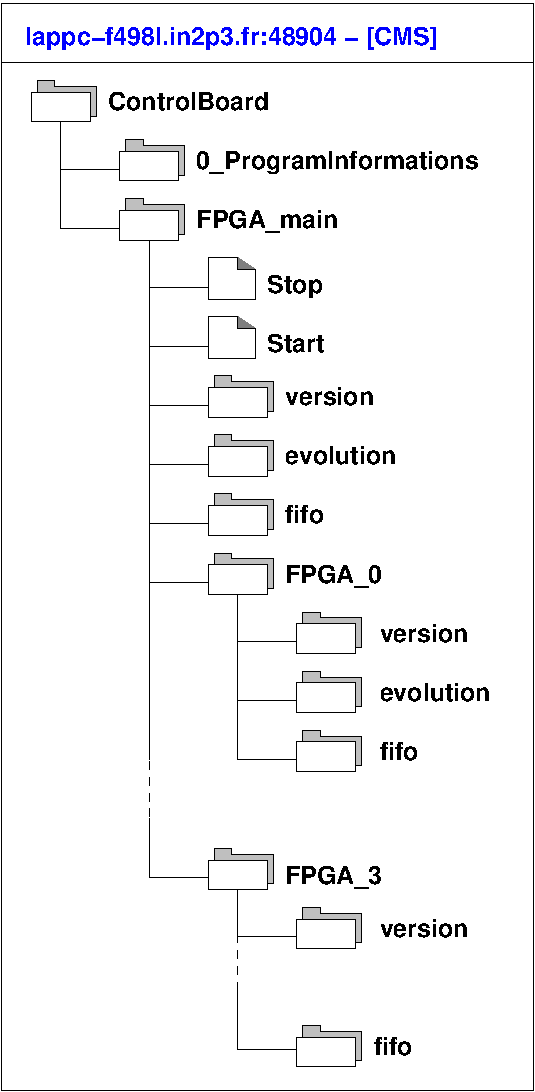
\includegraphics[width=5cm]{appendix/images/MOS_device_example_1.pdf}
\end{center}
\caption{Example of a  device managed through a MOS  server.  The root
  device is named \texttt{ControlBoard}.  First level daughter devices
  are  \texttt{0\_ProgramInformations} and  \texttt{FPGA\_main}.  Here
  the          MOS/OPCUA          server          is          labelled
  \texttt{CMS}.}\label{fig:an:mos_dev_1}
\end{figure}

% TODO


\subsection{Integration of a new device in the Vire environment}

The Vire  API also implements a  mechanism to describe a  hierarchy of
devices.  This  mechanism is independant  of the  one used in  the MOS
system but can  be easily made compatible with it.   This means that a
MOS  hierarchy  of devices  can  be  represented  in Vire.   The  Vire
hierarchy of  devices can  be considered as  some kind  of filesystem,
each device  being a folder with  its unique path, as  shown on figure
\ref{fig:an:mos_dev_2}.   The \emph{methods}  associated to  a devices
(or a datapoint) can be considered as plain executable files stored in
the  device's folder  : they  constitute the  set of  \emph{resources}
associated to the device.


\begin{figure}[h]
\begin{center}
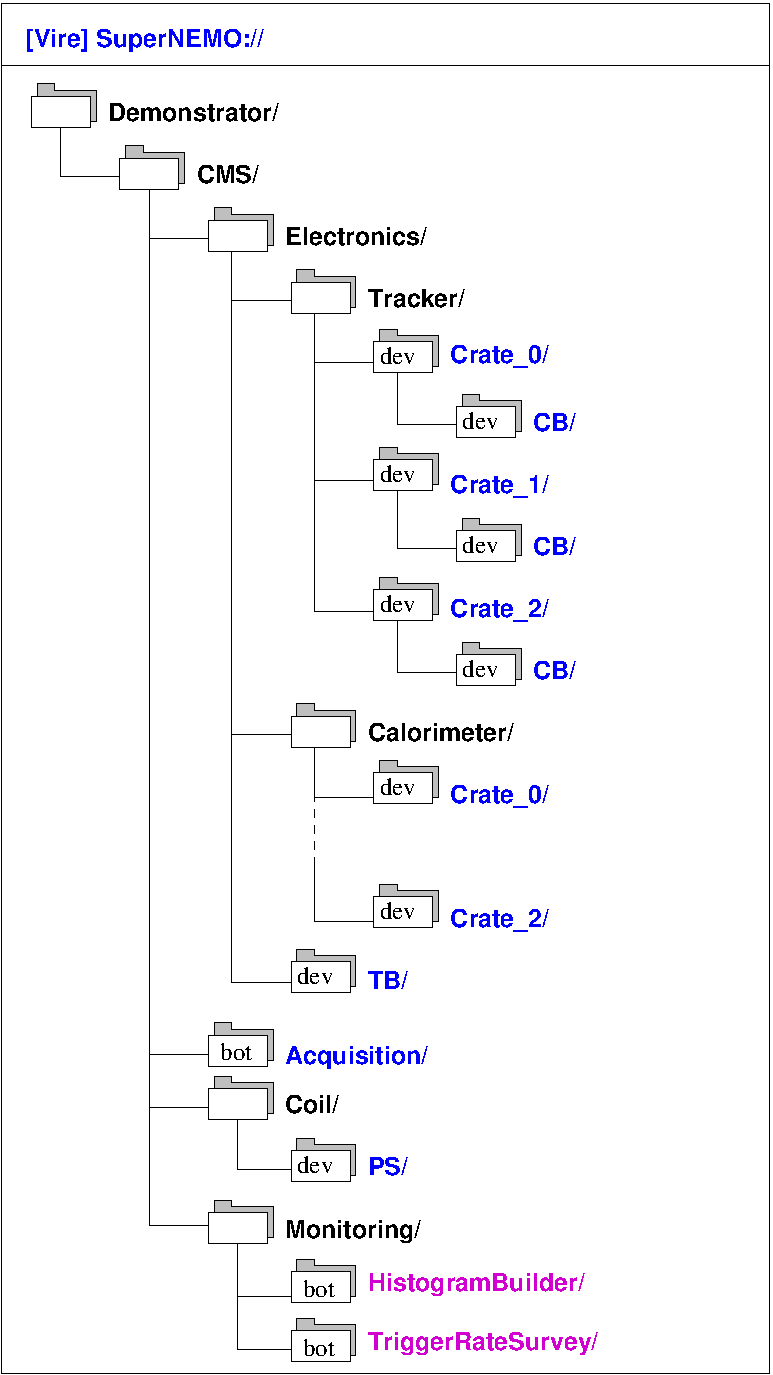
\includegraphics[width=5cm]{appendix/images/MOS_device_example_2.pdf}
\end{center}
\caption{Example of a hierarchy of  devices described by the Vire API.
  The root device is named  \texttt{SuperNEMO:}.  The top level (root)
  device  is  named  \texttt{Demonstrator}.  The  devices  colored  in
  \textcolor{blue}{blue}  are managed  through MOS/OPCUA.  The devices
  colored in \textcolor{magenta}{magenta} are directly embedded in the
  Vire server.  Devices with the \texttt{dev} tag are typical hardware
  device.  Devices  with the  \texttt{bot}  tag  are typical  software
  devices.   The  devices  colored in  \textbf{black}  are  structural
  pseudo-devices used to organize and  present a comprehensive view of
  the hierarchy. }\label{fig:an:mos_dev_2}
\end{figure}

The organisation of this hierarchy of devices is arbitrary and defined
by the designer of the  \emph{Control and Monitoring System}.  What is
important  to  understand  is  that  some  of  these  devices  can  be
associated  to  \emph{hardware  devices}  (a  power  supply  crate,  a
temperature probe\dots) and others  can be \emph{pseudo-devices}, i.e.
pure   software  object   (a   monitoring  robot,   a  file   transfer
daemon\dots).

In the context of the coupling of  the Vire server and the CMS server,
we are  in the event that  some devices are managed  by some MOS/OPCUA
servers and others are managed  in the Vire server itself.  Typically,
\emph{hardware devices}  are systematically managed through  the OPCUA
technology.  Vire has a mechanism to integrate such devices in its own
hierarchy.  This mechanism can  be considered like the \emph{mounting}
of   a   remote   filesystem   from  a   local   filesystem.    Figure
\ref{fig:an:mos_dev_0} illustrates  the case of many  hardware devices
-- managed by MOS -- that are integrated in the Vire system.  From the
Vire point of  view, the user does not see  the implementation details
for such  devices. He  does not  know the identity  of the  MOS server
hosting the device. He does not even know if the device is hosted by a
MOS server.  Devices are simply visible through the standard hierarchy
published by Vire with its  own device naming scheme, regardless their
true location.



\begin{figure}[h]
\begin{center}
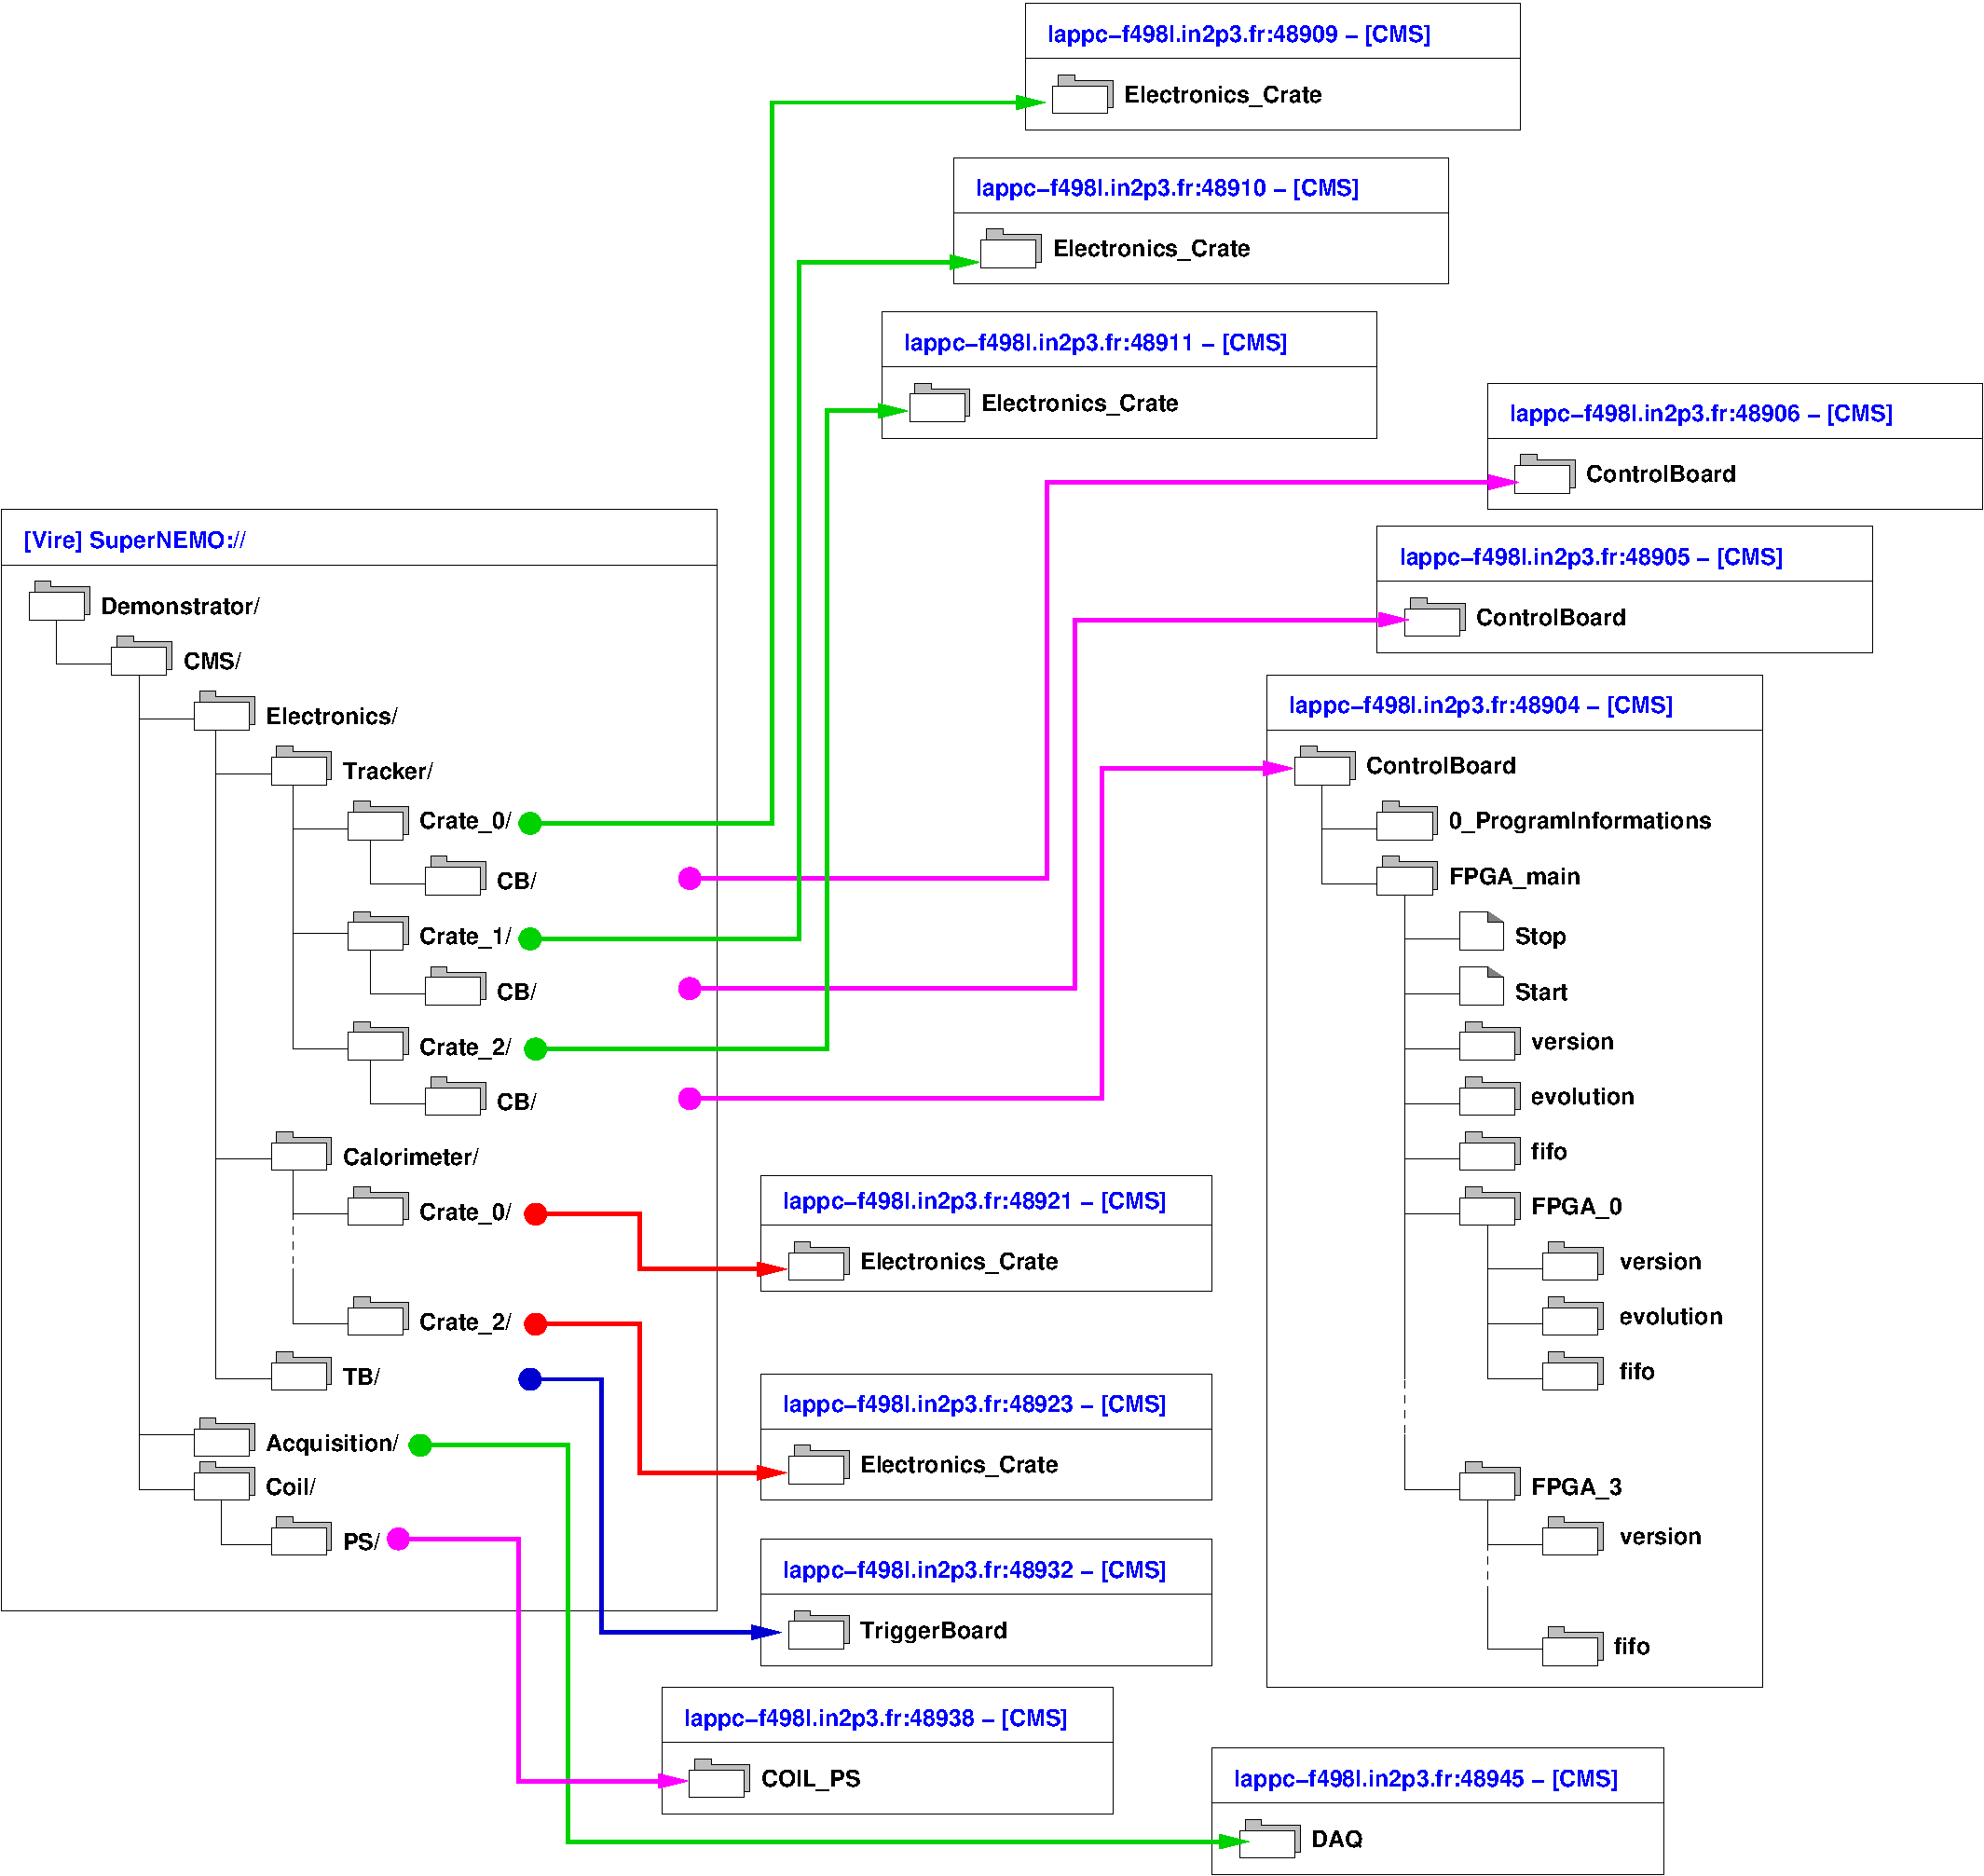
\includegraphics[width=\linewidth]{appendix/images/MOS_device_example_0.pdf}
\end{center}
\caption{The  mounting of  many  MOS device  hierarchies  in the  Vire
  device hierarchy.  Each OPCUA server  runs a simple  hardware device
  that is \emph{mounted} from a specific node with its own path.
%% of  devices described by the Vire API.
%%   The root device is named  \texttt{SuperNEMO:}.  The top level (root)
%%   device is  named \texttt{Demonstrator}. The devices  colored in blue
%%   are managed  through MOS/OPCUA. The  devices colored in  magenta are
%%   directly embedded in the Vire server.  Devices with the \texttt{dev}
%%   tag are typical  hardware device. Devices with  the \texttt{bot} tag
%%   are typical software devices.
}\label{fig:an:mos_dev_0}
\end{figure}




\subsection{Example}

Using  the examples  displayed  in  figure \ref{fig:an:mos_dev_0},  we
consider  in detail  the way  one specific  device managed  by MOS  is
mounted   in  the   Vire   hierarchy.  Figure   \ref{fig:an:mos_dev_3}
illustrates the mounting of a MOS device in Vire.

Here the Vire  server publishes the path of a  device representing the
control board  of the third  electronic crate  for the tracker  of the
SuperNEMO demonstrator module.  The full Vire path of this device is:

\textcolor{blue}{\texttt{SuperNEMO://Demonstrator/CMS/Electronics/Tracker/Crate\_2/CB}}

This is  the only Vire identifier  recognized by user to  address this
device.

On    the   figure,    one    can   see    that    the   MOS    server
\texttt{lappc−f498l.in2p3.fr} (port 48904) hosts a simple device which
is locally named \texttt{ControlBoard}.

When  mounting   this  device  in   the  Vire  hierarchy,   the  local
\texttt{[CMS]}  namespace and  \texttt{ControlBoard} device  names are
hidden and replaced by the Vire device path.  All daughter devices and
datapoints of  the \texttt{CMS/ControlBoard} device are  integrated as
daughters        of        the         Vire        device        named\\
\texttt{SuperNEMO://Demonstrator/CMS/Electronics/Tracker/Crate\_2/CB}.


For example, the \texttt{FPGA\_main} daughter device is now associated
to the following Vire path:

\textcolor{blue}{\texttt{SuperNEMO://Demonstrator/CMS/Electronics/Tracker/Crate\_2/CB/FPGA\_main/}}

and  its  \texttt{Stop} method  is  automatically  addressed with  the
following \emph{leaf} path:

\textcolor{blue}{\texttt{SuperNEMO://Demonstrator/CMS/Electronics/Tracker/Crate\_2/CB/FPGA\_main/Stop}}


\begin{figure}[h]
\begin{center}
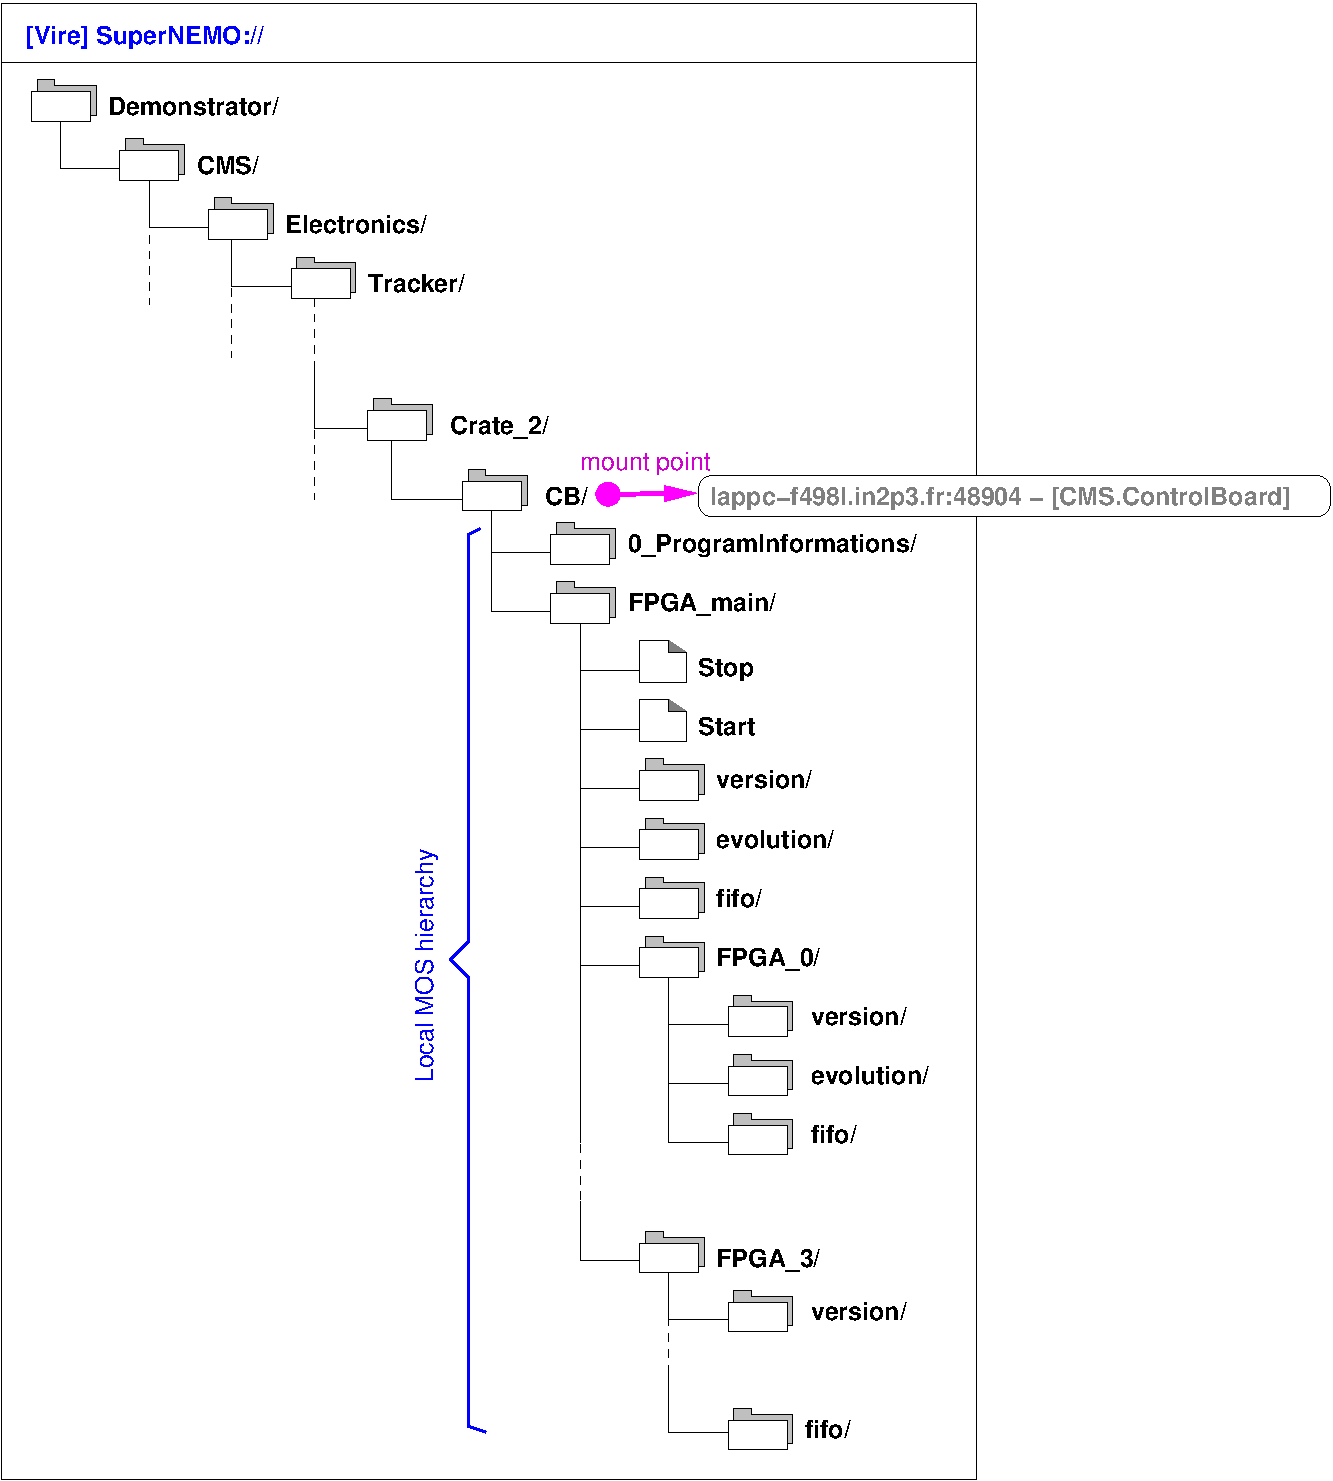
\includegraphics[width=0.8\linewidth]{appendix/images/MOS_device_example_3.pdf}
\end{center}
\caption{The  mounting of  one  MOS device and its local hierarchy  in the  Vire
  device hierarchy.}\label{fig:an:mos_dev_3}
\end{figure}



\subsection{Vire/MOS mapping}

As it can be  seen in the above example, the integration  of a new MOS
device in the Vire system is  achieved through soem kind of filesystem
mounting operation.   Particularly, it is  shown that the MOS  name of
the   mounted  root   device  is   replaced  by   an  arbitrary   Vire
path. However, all daughter  nodes (devices, datapoints) attached from
this root  node have their  relative MOS  names preserved in  the Vire
naming scheme.

Any  resource  (method)  associated  to any  of  such  daughter  nodes
inherits this relative naming scheme.

As Vire applications  describe resources through their  Vire paths, it
is thus needed to build an explicit map that associates resource paths
to MOS address  and name. The CMS  server will be able  to resolve the
MOS server/port and  embedded device associated to  the resource path.

The goal of the \texttt{devices\_launch.conf} file is not only to tell
the CMS server what MOS server should  be loaded and ran at start, but
also  to describe  the  \emph{mounting point/names}  used  by Vire  to
access the resources associated to MOS devices.  From the informations
stored in the  file, an explicit associative array must  be built when
the Vire server connect to the CMS server.  It will play the role of a
resource path resolver  when requests about resources will  be sent by
Vire applications.  This associative array  must be locked  during the
Vire/CMS connection.



%\subsubsection{Preparation of XML device models}

%% \noindent\underline{Pre-condition:}
%% The device is working and validated through the MOS/OPCUA server

%% \begin{enumerate}

%% \item Produce XML décrivant le modèle du device enrichi
%%   des metadata
%% Rédaction du fichier XML décrivant le modèle du device

%% \item Génération des fichiers model du type de device pour Vire

%% \item Génération des fichiers instances resolv.conf

%% \end{enumerate}


\vfill
\pagebreak
\clearpage

% end


\section{Vire messages}\label{app:vire_messages}

Within Vire  and between Vire  components and external  components, we
use  a communication  system  based on  Vire  messages.  This  section
describes the structure of such messages.

\subsection{General structure of a message}

Each message consists in two parts (figure \ref{fig-vire-message-message-cpp}):
\begin{itemize}

\item  the  \emph{header}  is   dedicated  to  generic  and  typicalle
  mandatory  informations  which  document   the  message  itself  and
  arbitrary high-level metadata.

\item  the \emph{body}  of the  message  contains the  real data: the payload.
  The structure of the message body depends on some convention. Vire uses
  its own convention to embed the payload data.

\end{itemize}

\begin{figure}[h]
\vskip 10pt
\small
\begin{Verbatim}[frame=single,xleftmargin=0.cm,label=\fbox{C++}]
struct vire::message::message {
  message_header header; // Header of the message
  message_body   body;   // Body of the message
};
\end{Verbatim}
\normalsize
\caption{The structure of a Vire message object (C++  class:
  \texttt{"vire::message::message"})}\label{fig-vire-message-message-cpp}
\end{figure}

\subsection{The message header}

The header contains (figure \ref{fig-vire-message-message_header-cpp}):
\begin{itemize}

  \item The mandatory \texttt{message\_id}  attribute is an identifier
    of the  message which  document the emitter  and a  unique message
    number.   Each emitter  is  responsible of  the  numbering of  the
    messages it  emits, typically using an  incremental technique. The
    message  number is  a positive  integer, starting  from 0  (figure
    \ref{fig-vire-message-message_identifier-cpp}).

  \item  The \texttt{timestamp}  attribute  encodes the  approximative
    time point when the message was  created. It contains the date and
    the time, using at least microsecond resolution.

    Typically,  with  JSON  encoding  system, it  is  expected  to  be
    formatted as a character string, using the following ISO format:

    \begin{center}
      \texttt{yyyymmddThhmmss.uuuuuu}
    \end{center}

    \noindent where:

    \vskip -10pt
    \begin{itemize}
    \item[\texttt{yyyymmdd} :] encodes year/month/day,
    \item[\texttt{hhmmssd} :] encodes hour/minute/second,
    \item[\texttt{uuuuuu} :] encodes microseconds.
    \end{itemize}

  \item   In   the   case    of   a   \emph{response}   message,   the
    \texttt{in\_reply\_to} attribute is set to identify the associated
    request message.

  \item  The \texttt{asynchronous}  boolean  attribute is  set if  the
    message processing  is explicitely requested  by the source  to be
    asynchronous (non-blocking).  In  RPC transactions, where requests
    are transmitted from one point to  the other, its default value is
    \emph{false}.   It  is possible  to  force  a RPC  transaction  in
    asynchronous mode.   This use  case is documented  elsewhere.  For
    event messaging, this flag is conventionally set to \emph{true}.

  \item  The  \texttt{body\_layout\_id}  attribute  is  the  mandatory
    identifier   of   the   layout   of  the   message   body   (class
    \texttt{"vire::utility::model\_identifier"}).  The  default layout
    for     message     body     inside    the     Vire     API     is
    \texttt{"vire::message::body\_format::typed\_payload"}, with version
    \texttt{"1.0"}                                             (figure
    \ref{fig-vire-utility-model_identifier-cpp}).

\end{itemize}


\begin{figure}[h]
\vskip 10pt
\small
\begin{Verbatim}[frame=single,xleftmargin=0.cm,label=\fbox{C++}]
struct vire::message::message_header {
  message_identifier message_id;     // Message identifier from the emitter.
  std::string        timestamp;      // Timestamp.
  message_identifier in_reply_to;    // Message identifier of the associated
                                     // request message (optional).
  bool               asynchronous,   // Asynchronous flag.
  vire::utility::model_identifier     body_layout_id; // Body layout identifier.
  std::map<std::string, std::string>  metadata;       // Key/value metadata dictionary.
};
\end{Verbatim}
\normalsize
\caption{The  structure  of  a   message  header  object  (C++  class:
  \texttt{"vire::message::message\_header"}).}\label{fig-vire-message-message_header-cpp}
\end{figure}

\begin{figure}[h]
\vskip 10pt
\small
\begin{Verbatim}[frame=single,xleftmargin=0.cm,label=\fbox{C++}]
struct vire::message::message_identifier {
  std::string emitter; // Name identifying the emitter of the message.
  int32_t     number;  // Number identifying the message in the emitter's
                       // message numbering scheme.
};
\end{Verbatim}
\normalsize
\caption{The      structure      of     a      message      identifier
  (C++  class:  \texttt{"vire::message::message\_identifier"}).}
\label{fig-vire-message-message_identifier-cpp}
\end{figure}

\begin{figure}[h]
\vskip 10pt
\small
\begin{Verbatim}[frame=single,xleftmargin=0.cm,label=\fbox{C++}]
struct vire::utility::model_identifier {
  std::string name;    // Name identifying the format of the message.
  std::string version; // String identifying the version of the format.
};
\end{Verbatim}
\normalsize
\caption{The structure of a model identifier (C++  class:  \texttt{"vire::utility::model\_identifier"}.}\label{fig-vire-utility-model_identifier-cpp}
\end{figure}




\begin{figure}[h]
\vskip 10pt
\small
\begin{Verbatim}[frame=single,xleftmargin=0.cm,label=\fbox{JSON}]
{
   "header" : {
      "message_id" : {
         "emitter" : "vire.server",
         "number" : 42
      },
      "timestamp" : "20160930T141408.413443",
      "in_reply_to" : {
         "initialized" : true,
         "value" : {
            "emitter" : "vire.client.0",
            "number" : 23
         }
      },
      "asynchronous" : false,
      "body_layout_id" : {
         "name" : "vire::message::body_format::typed_payload",
         "version" : {
            "initialized" : true,
            "value" : "1.0"
         }
      },
      "metadata" : [
         {
            "key" : "key1",
            "value" : "foo"
         },
         {
            "key" : "key2",
            "value" : "42"
         },
         {
            "key" : "key3",
            "value" : "3.1415899999999999"
         },
         {
            "key" : "key4",
            "value" : "true"
         }
      ]
   }
  "body" : {
      ...
   }
}
\end{Verbatim}
\normalsize
\caption{Example of  a   message  header  object in JSON format.}
\label{fig-vire-message-message_header-json}
\end{figure}

\vfill
\clearpage
\pagebreak

\subsection{The message body}

The    default    message   body    layout    in    Vire   is    named
\texttt{"vire::message::body\_format::typed\_payload"}        (version
\texttt{"1.0"}).   Each  message used  within  the  Vire framework  is
supposed to use this layout.  The general idea is that the body of the
message embeded the  \emph{payload object} that has  to be transmitted
between  two components  of  the system.   \emph{Payload objects}  are
classified in one of the three following categories:

\begin{enumerate}

\item \emph{Request}:  describes a request submitted  by one component
  to another component (generally during a synchronous RPC transaction).

\item  \emph{Response}: describes  the  response to  a former  request
  (generally during a synchronous RPC transaction).

\item \emph{Event}: describes an  arbitrary information record (alarm,
  exception, signal\dots) which is transmitted asynchronously.

\end{enumerate}

Vire implements the following class hierarchy:

\begin{center}
\begin{tikzpicture}
  \node (payload)  at (0,2)  [draw] {\texttt{vire::utility::base\_payload}};
  \node (request)  at (-4,0) [draw] {\texttt{vire::utility::base\_request}};
  \node (response) at (2,0)  [draw] {\texttt{vire::utility::base\_response}};
  \node (event)    at (8,0)  [draw] {\texttt{vire::utility::base\_event}};

  %\draw[style=help lines] (-3,-1) grid (10,4);
  \draw (node cs:name=response,anchor=north) |- (0,1);
  \draw (node cs:name=event,anchor=north)    |- (0,1);
  \draw[->] (node cs:name=request,anchor=north)
  |- (0,1) -| (node cs:name=payload,anchor=south);
\end{tikzpicture}
\end{center}

The requirements for the transmitted object are the following:

\begin{itemize}

\item The  type of the object  must be conventionally associated  to a
  unique     \emph{model      identifier}     object      (see     the
  \texttt{"vire::utility::model\_identifier"} class)  which contains a
  unique   name   (\textit{string    identifier})   and   possibly   a
  \textit{version identifier}.  Each software  component that may send
  or  receive the  object  should agree  on  this type  identification
  scheme.   This   enable  the  use  of   object  factories,  whatever
  programming  langage  is used  on  both  side of  the  communication
  system.

\item  For each  software component,  the object  type must  have some
  dedicated  encoding/decoding  functions  available  (again  whatever
  programming language is used). For example the Vire API supports the
  following encoding formats:

  \begin{itemize}

  \item JSON (MIME  encoding type: \texttt{"application/x-json"}), which
    is supportable by many languages,

  \item  Protobuf  (Google  Protocol   Buffers,  MIME  encoding  type:
    \texttt{"application/x-protobuf"}), which is also widely supported,

  \item   Boost/serialisation   (XML,    text   or   binary   archives
    \texttt{"application/x-boost-serialization-xml"},
    \texttt{"application/x-boost-serialization-text"},
    \texttt{"application/x-boost-serialization-binary"}),    which    in
    principle is supported by C++ only.

  \end{itemize}

  The Protobuf  encoding format will be  used to serialize/deserialize
  the  Vire  messages transported  between  the  Vire server  and  the
  CMS/LAPP server.

\end{itemize}

Vire uses a dedicated layout to represent the body of any message with
its embedded payload object. With this technique, the structure of the
body          contains         two          attributes         (figure
\ref{fig-app-vire-message-message_body-cpp}):

\begin{enumerate}

\item The \texttt{payload\_type\_id} specifies the type of the payload
  object   (figure   \ref{fig-app-vire-utility-model_identifier-cpp}).
  This unique name  is conventionaly fixed for a  given application. A
  version tag allows to support possible evolution of the object type.

\item The  \texttt{payload} is a  handle to  a payload object  of type
  request, response or event.

  %% \begin{itemize}
  %% \item Within  the producer  component of  the message,  the encoding
  %%   function associated to the object  type is responsible to generate
  %%   the JSON stream for the object and store it in the buffer.

  %% \item Within  the consumer  component of  the message,  the decoding
  %%   function associated to the object type is responsible to parse the
  %%   JSON stream stored in the buffer and restore the object in memory.

  %% \end{itemize}

  It is expected  that, on both sides of the  connection, the software
  components can  access dedicated  software plugins which  ensure the
  support  of  various   \emph{payload  object  types}  conventionnaly
  associated  with  their  \emph{payload type  identifiers}  and  also
  providing JSON and/or Protobuf encoding/decoding functionalities.

  %% The   system  allows  to  support
  %% modification  in the  structure of  the objects  thanks to  version
  %% tagging.

\end{enumerate}

\begin{figure}[h]
\vskip 10pt
\small
\begin{Verbatim}[frame=single,xleftmargin=0.cm,label=\fbox{C++}]
struct message_body {
  vire::utility::model_identifier     payload_type_id; // Object type identifier.
  const vire::utility::base_payload * payload;         // Handle to a payload object.
};
\end{Verbatim}
\normalsize
\caption{The structure of a message body object (C++).}
\label{fig-app-vire-message-message_body-cpp}
\end{figure}

\begin{figure}[h]
\vskip 10pt
\small
\begin{Verbatim}[frame=single,xleftmargin=0.cm,label=\fbox{JSON}]
{
  "header" : {
    ...
  },
  "body" : {
    "payload_type_id" : {
      "name" : "vire::message::testing::error_event",
      "version" : {
        "initialized" : false
      }
    },
    "payload" : {
      "timestamp" : "20160930T141743.759085"
      "err" : {
        "code" : 3,
        "message" : "A basic error"
      },
    }
  }
}
\end{Verbatim}
\normalsize
\caption{Example of  a   message  body  object in JSON format.}
\label{fig-vire-message-message_body-json}
\end{figure}

\vfill
\clearpage
\pagebreak

% end

%\input{appendix/app_json_fmt.tex}

\section{The \emph{Protocol Buffers} format}\label{app:protobuf_fmt}

\subsection{Introduction}

The  Google  Protocol Buffers  (\emph{protobuf})  library  is used  to
represent the objects that are exchanged between the Vire clients, the
Vire server and the CMS server.  The  version 3 of the format is used,
implying   at   least   version   3.0.0  (September   2016)   of   the
\emph{protobuf} library.

Each  data   structure  of  interest   can  be  described   through  a
\texttt{.proto}  file  from  which  stub files  can  be  automatically
generated  with the  \texttt{protoc} compiler.  For Vire  and its  CMS
interface, the C++ and Java programming languages will be used.


A  collection of  \texttt{.proto}  files are  provided  with the  Vire
library to represent all kind  of data structures transferable between
networked agents  (Vire server,  Vire clients, CMS/LAPP  server).  The
objects of  the highest level  are named \emph{payload  objects} (like
\emph{request},  \emph{response} and  \emph{event} objects).   They
are composed of attributes of more basic data structures.

\subsection{Example}

The following  class diagram  illustrates two data  structures defined
within the Vire library with an inheritance relationship between them.

\begin{center}
  \begin{tikzpicture}
    \node (base)     at (0,1.5)  [draw] {\texttt{vire::utility::base\_error}};
    \node (setup)    at (0,0)  [draw] {\texttt{vire::utility::invalid\_setup\_id\_error}};

    \draw[->]   (node cs:name=setup,anchor=north) |- (0,1);
    |- (0,1) -| (node cs:name=base,anchor=south);
  \end{tikzpicture}
\end{center}

The \texttt{vire::utility::base\_error}  is the  parent class  for all
\emph{error}  objects.   It  contains   two  attributes:   an  integer
\emph{error code}  and a  character string describing  the \emph{error
  message}.

The   \texttt{vire::utility::invalid\_setup\_id\_error}  class   is  a
specialized error class  which represents explicitely an  error due to
an identification  failure of  the experimental setup.   It implements
additional mutually exclusive attributes: the \emph{unrecognized name}
of the setup or the \emph{unrecognized version} of the setup.

This   example  illustrates   the  protobuf   representation  of   the
\texttt{vire::utility::base\_error}  in the  Vire  library, using  the
\texttt{"vire/utility/BaseError.proto"} file:

\small
\begin{Verbatim}[frame=single,xleftmargin=0.cm,label=\fbox{protobuf}]
  syntax = "proto3";
  package vire.utility; // Namespace

  message BaseError {

    // reserved 1; // Reserved for _base message

    // Attributes:
    int32  code           = 100; // The error code
    string message_format = 101; // The error description message

  }
\end{Verbatim}
\normalsize

\vfill
\clearpage
\pagebreak

\subsection{Vire protobuf conventions}

Vire uses the following conventions:

\begin{enumerate}

\item
  The member index  \texttt{1} is reserved to represent the  link of a
  class to its main base/parent class (if any).  It is not used if the
  data structure does not inherit any data structure.
  If a data structure naturally inherits another one, it is thus possible
  to  represent the  inheritance  relationship as  illustrated with  the
  \texttt{"vire/utility/InvalidSetupIdError.proto"}      file      which
  represents the \texttt{vire::utility::invalid\_setup\_id\_error} class
  in the Vire library:

  \small
  \begin{Verbatim}[frame=single,xleftmargin=0.cm,label=\fbox{protobuf}]
    syntax = "proto3";
    package vire.utility; // Namespace

    import "vire/utility/BaseError.proto"; // Dependency

    message InvalidSetupIdError {

      BaseError _base = 1; // The base class

      // Additional attributes:
      oneof detail { // Mutual exclusion
        string invalid_setup_name    = 100; // The failed setup name
        string invalid_setup_version = 101; // The failed setup version
      }

    }
  \end{Verbatim}
  \normalsize

\item The  \texttt{\_base} member  is conventionally  used to  represent the
  inheritance   relationship    from   a   data   structure    of   type
  \texttt{"vire.utility.BaseError"}.

\item Member indexes from \texttt{2}  to \texttt{99} are also reserved
  for possible future usage (multiple inheritance, metadata\dots).

\item
  The first member of the data structure must start at index \texttt{100}.

\end{enumerate}

\vfill
\clearpage
\pagebreak

% end


\section{Vire payload objects}\label{app:payload}

\subsection{Introduction}

As  mentioned in  appendix \ref{app:protobuf_fmt},  Vire messages  are
wrappers for \emph{payload objects}.  Each  type of payload object can
be represented  through the \emph{protobuf} mechanism.   The following
class hierarchy shows the base architecture used to define new payload
objects.

\begin{center}
\begin{tikzpicture}
  \node (payload)  at (0,2)   [draw] {\texttt{vire::utility::base\_payload}};
  \node (request)  at (-4,0)  [draw] {\texttt{vire::utility::base\_request}};
  \node (response) at (2,0)   [draw] {\texttt{vire::utility::base\_response}};
  \node (event)    at (8,0)   [draw] {\texttt{vire::utility::base\_event}};
  \node (my)       at (-4,-2) [draw] {\texttt{my\_request}};
  \node (your)     at (2,-2)  [draw] {\texttt{your\_response}};
  \node (its)    at (8,-2)    [draw] {\texttt{its\_alarm}};

  %\draw[style=help lines] (-6,-2) grid (10,2);
  \draw (node cs:name=response,anchor=north) |- (0,1);
  \draw (node cs:name=event,anchor=north)    |- (0,1);
  \draw[->] (node cs:name=request,anchor=north)
  |- (0,1) -| (node cs:name=payload,anchor=south);
  \draw[->] (node cs:name=my,anchor=north)
  |- (-4,-1) -| (node cs:name=request,anchor=south);
  \draw[->] (node cs:name=your,anchor=north)
  |- (2,-1) -| (node cs:name=response,anchor=south);
  \draw[->] (node cs:name=its,anchor=north)
  |- (8,-1) -| (node cs:name=event,anchor=south);
\end{tikzpicture}
\end{center}


\begin{center}
\vskip 10pt
\small
\begin{tabular}{|l|l|l|}
  \hline
  \textbf{Vire C++ class} & \textbf{protobuf message type} & \textbf{protobuf definition file} \\
  \hline
  \hline
  \multicolumn{3}{|c|}{\emph{general types}} \\
  \hline
  boost::posix\_time::ptime & google.protobuf.Timestamp & google/protobuf/timestamp.proto \\
  \hline
  \hline
  \multicolumn{3}{|c|}{\emph{identifier types}} \\
  \hline
  vire::utility::base\_identifier & vire.utility.Baseidentifier & vire/utility/Baseidentifier.proto \\
  \hline
  vire::utility::instance\_identifier & vire.utility.InstanceIdentifier & vire/utility/InstanceIdentifier.proto \\
  \hline
  vire::utility::model\_identifier & vire.utility.ModelIdentifier & vire/utility/ModelIdentifier.proto \\
  \hline
  \hline
  \multicolumn{3}{|c|}{\emph{error types}} \\
  \hline
  vire::utility::base\_error & vire.utility.BaseError & vire/utility/BaseError.proto \\
  \hline
  vire::utility::invalid\_context\_error & vire.utility.InvalidContextError & vire/utility/InvalidContextError.proto \\
  \hline
  vire::utility::invalid\_setup\_id\_error & vire.utility.InvalidSetupIdError & vire/utility/InvalidSetupIdError.proto \\
  \hline
  \hline
  \multicolumn{3}{|c|}{\emph{payload types}} \\
  \hline
  vire::utility::base\_payload & vire.utility.BasePayload & vire/utility/BasePayload.proto \\
  \hline
  vire::utility::base\_request & vire.utility.BaseRequest & vire/utility/BaseRequest.proto \\
  \hline
  vire::utility::base\_response & vire.utility.BaseResponse & vire/utility/BaseResponse.proto \\
  \hline
  vire::utility::base\_event & vire.utility.BaseEvent & vire/utility/BaseEvent.proto \\
  \hline
  vire::utility::base\_alarm & vire.utility.BaseAlarm & vire/utility/BaseAlarm.proto \\
  \hline
  \hline
  \multicolumn{3}{|c|}{\emph{messenging types}} \\
  \hline
  vire::message::message\_identifier & vire.message.MessageIdentifier & vire/message/MessageIdentifier.proto \\
  \hline
  vire::message::msg\_header & vire.message.MsgHeader & vire/message/MsgHeader.proto \\
  \hline
  vire::message::msg\_body & vire.message.MsgBody & vire/message/MsgBody.proto \\
  \hline
  vire::message::message & vire.message.Message & vire/message/Message.proto \\
  \hline
\end{tabular}
\normalsize
\end{center}


\begin{center}
\vskip 10pt
\small
\begin{tabular}{|l|l|l|}
  \hline
  \multicolumn{3}{|c|}{\emph{Resource management related types}} \\
  \hline
  vire::cms::resource\_status\_record & vire.cms.ResourceStatusRecord & vire/cms/ResourceStatusRecord.proto \\
  \hline
  vire::cms::resource\_fetch\_status\_request & vire.cms.ResourceFetchStatusRequest & vire/cms/ResourceFetchStatusRequest.proto \\
  \hline
  vire::cms::resource\_fetch\_status\_success\_response & vire.cms.ResourceFetchStatusSuccessResponse & vire/cms/ResourceFetchStatusSuccessResponse.proto \\
  \hline
  vire::cms::resource\_fetch\_status\_failure\_response & vire.cms.ResourceFetchStatusFailureResponse & vire/cms/ResourceFetchStatusFailureResponse.proto \\
  \hline
  vire::cms::resource\_exec\_request & vire.cms.ResourceExecRequest & vire/cms/ResourceExecRequest.proto \\
  \hline
  vire::cms::resource\_exec\_success\_response & vire.cms.ResourceExecSuccessResponse & vire/cms/ResourceExecSuccessResponse.proto \\
  \hline
  vire::cms::resource\_exec\_failure\_response & vire.cms.ResourceExecFailureResponse & vire/cms/ResourceExecFailureResponse.proto \\
  \hline
  vire::cms::resource\_exec\_non\_blocking\_request & vire.cms.ResourceExecNonBlockingRequest & vire/cms/ResourceExecNonBlockingRequest.proto \\
  \hline
  vire::cms::resource\_exec\_non\_blocking\_ack\_response & vire.cms.ResourceExecNonBlockingAckResponse & vire/cms/ResourceExecNonBlockingAckResponse.proto \\
  \hline
  vire::cms::resource\_exec\_non\_blocking\_noack\_response & vire.cms.ResourceExecNonBlockingNoackResponse & vire/cms/ResourceExecNonBlockingNoackResponse.proto \\
  \hline
  vire::cms::resource\_exec\_non\_blocking\_success\_event & vire.cms.ResourceExecNonBlockingSuccessEvent & vire/cms/ResourceExecNonBlockingSuccessEvent.proto \\
  \hline
  vire::cms::resource\_exec\_non\_blocking\_failure\_event & vire.cms.ResourceExecNonBlockingFailureEvent & vire/cms/ResourceExecNonBlockingFailureEvent.proto \\
  \hline
  vire::cms::resource\_exec\_error & vire.cms.ResourceExecError & vire/cms/ResourceExecError.proto \\
  \hline
  vire::cms::invalid\_status\_error & vire.cms.ResourceExecError & vire/cms/ResourceExecError.proto \\
  \hline
  %% vire::cms::invalid\_credentials\_error & vire.cms.InvalidCredentialsError & vire/cms/InvalidCredentialsError.proto \\
  %% \hline
  %% vire::cms::invalid\_user\_error & vire.cms.InvalidUserError & vire/cms/InvalidUserError.proto \\
  %% \hline
  vire::cms::invalid\_resource\_error & vire.cms.InvalidUserError & vire/cms/InvalidUserError.proto \\
  \hline
  vire::cms::no\_pubsub\_resource\_error & vire.cms.NoPubsubResourceError & vire/cms/NoPubsubResourceError.proto \\
  \hline
  \hline
  \multicolumn{3}{|c|}{\emph{Resource pub/sub management types}} \\
  \hline
  vire::cms::resource\_pubsub\_subscribe\_request & vire.cms.ResourcePubsubSubscribeRequest & vire/cms/ResourcePubsubSubscribeRequest.proto \\
  \hline
  vire::cms::resource\_pubsub\_subscribe\_success\_response & vire.cms.ResourcePubsubSubscribeRSuccessResponse & vire/cms/ResourcePubsubSubscribeRSuccessResponse.proto \\
  \hline
  vire::cms::resource\_pubsub\_subscribe\_failure\_response & vire.cms.ResourcePubsubSubscribeRFailureResponse & vire/cms/ResourcePubsubSubscribeRSuccessResponse.proto \\
  \hline
  \hline
  \multicolumn{3}{|c|}{\emph{Vire/CMS server interface types}} \\
  \hline
  vire::cmsinterface::connection\_request & vire.cmsinterface.ConnectionRequest & vire/cmsinterface/ConnectionRequest.proto \\
  \hline
  vire::cmsinterface::connection\_success\_response & vire.cmsinterface.ConnectionSuccessResponse & vire/cmsinterface/ConnectionSuccessResponse.proto \\
  \hline
  vire::cmsinterface::connection\_failure\_response & vire.cmsinterface.ConnectionFailureResponse & vire/cmsinterface/ConnectionFailureResponse.proto \\
  \emph{embedded:} unknown\_resources\_error & .UnknownResourcesError &  \\
  \hline
  vire::cmsinterface::disconnection\_request & vire.cmsinterface.DisconnectionRequest & vire/cmsinterface/DisconnectionRequest.proto \\
  \hline
  vire::cmsinterface::disconnection\_success\_response & vire.cmsinterface.DisconnectionSuccessResponse & vire/cmsinterface/DisconnectionSuccessResponse.proto \\
  \hline
  %% \hline
  %% vire::cmsinterface::disconnection\_failure\_response & vire.cmsinterface.DisconnectionFailureResponse & vire/cmsinterface/DisconnectionFailureResponse.proto \\
\end{tabular}
\normalsize
\end{center}

\subsection{Basic data structures}

Any  payload object  (request, response  or event)  generally contains
some information records which are  specific to the functionalities of
the  payload  object they  belong.   These  records are  of  arbitrary
types. Of course they should be  translatable in terms of the protobuf
library.
%Of course they can be (de)serialized using JSON.
Some of these types are very  general and defined within the Vire core
API itself because they are reused by various payload objects not only
through  the Vire-CMS/LAPP  interface  but also  between  Vire clients  and
servers, independently  of the  CMS/LAPP server.  However,  the use  of the
Protocol Buffers interface makes possible  to publish the interface of
such data to the outside world, including the CMS/LAPP server in priority.

%% Other one are specific to the Vire/CMS interface and thus managed only
%% in the \texttt{Vire\_CMSInterface} API.
These  types  are considered  as  \emph{basic}.  Among them  we  find:
generic error  types, generic  identifier types,  timestamps, resource
status records\dots We propose to describe them in this section.

Once a sufficient collection of  basic data record types is available,
it  is possible  to describe  high  level payload  object types  which
aggregate attributes of such types.

Other record  types are specific to  some payload objects and  will be
never  used outside  the scope  of these  payload objects.   Such data
structures will be  explicitely declared with the  payload object they
belong to, likely as embedded types/classes.


\subsubsection{Errors}

Some  \emph{response} or  \emph{event} payload  objects may  contain a
specific  error  record  object.   A  \emph{failure  response}  or  an
\emph{exception  event}  object will  generally  embed  such an  error
record object.

Each  \emph{error record}  is represented  by an  instance of  a given
error type.   Each of  the error  types defined  in Vire  inherits the
\texttt{vire::utility::base\_error}      base       class      (figure
\ref{fig-app-payload-base_error})   which   contains   the   following
attributes:

\begin{itemize}

\item the error code: A non zero  integer which is set to 1 by default
  (indicating  a  generic  failure  case).   The  error  code  can  be
  conventionally  set to  any positive  integer value  to represent  a
  specific error case, depending on the context.

\item the error  message: an optional human  readable character string
  which documents the error as usefully as possible.

\end{itemize}

\begin{figure}[h]
\vskip 10pt
\small
\begin{Verbatim}[frame=single,xleftmargin=0.cm,label=\fbox{C++}]
struct vire::utility::base_error
{
  // Attributes:
  int         code;           // Error code (>0).
  std::string message_format; // Error message (optional).
};
\end{Verbatim}
\normalsize
\caption{The structure of a \texttt{"vire::utility::base\_error"} object
  (C++).}
\label{fig-app-payload-base_error}
\end{figure}


%% An example of JSON formatted basic error object is given in figure
%% \ref{fig-app-payload-base_error-1}.
%%
%% \begin{figure}[h]
%% \vskip 10pt
%% \small
%% \begin{Verbatim}[frame=single,xleftmargin=0.cm,label=\fbox{\texttt{JSON}}]
%% {
%%   "code" : "42",
%%   "message_format" : "Invalid AMQP server port=[2341]"
%% }
%% \end{Verbatim}
%% \normalsize
%% \caption{JSON  formatted  basic  error  object  (class
%%   \texttt{vire::utility::base\_error}.}
%% \label{fig-app-payload-base_error-1}
%% \end{figure}

Several type of generic errors are defined in Vire:


\begin{center}
\begin{tikzpicture}
  \node (base)     at (0,2)  [draw] {\texttt{vire::utility::base\_error}};
  \node (context)  at (-4,0) [draw] {\texttt{vire::utility::invalid\_context\_error}};
  \node (setup)    at (0,-1)  [draw] {\texttt{vire::utility::invalid\_setup\_id\_error}};
  \node (resource) at (4,0)  [draw] {\texttt{vire::cms::invalid\_resource\_error}};
  \node (user)     at (8,-1)  [draw] {\texttt{vire::cms::invalid\_user\_error}};

  \draw     (node cs:name=setup,anchor=north)    |- (0,1);
  \draw     (node cs:name=resource,anchor=north) |- (0,1);
  \draw     (node cs:name=user,anchor=north)     |- (0,1);
  \draw[->] (node cs:name=context,anchor=north)
  |- (0,1) -| (node cs:name=base,anchor=south);
\end{tikzpicture}
\end{center}

\noindent
Here are a few error object types defined in Vire.  Some types belongs
to the \texttt{utility} namespace, other  ones are in the \texttt{cms}
namespace:

\begin{itemize}

\item \texttt{"vire::utility::invalid\_context\_error"} : occurs typically when
  the general context of the execution of a given resource is not adapted.\\
  It is mapped to the \texttt{"vire.utility.InvalidContextError"} protobuf record.

\item \texttt{"vire::utility::invalid\_setup\_id\_error"} : occurs in case
  of an invalid identification of the experimental setup managed
  by the Vire or CMS server.\\
  It is mapped to the \texttt{"vire.utility.InvalidSetupIdError"} protobuf record.

\item \texttt{"vire::cms::invalid\_resource\_error"} : occurs in case
  of an invalid identification of a resource.\\
  It is mapped to the  \texttt{"vire.cms.InvalidResourceError"} protobuf record.

\item \texttt{"vire::cms::invalid\_status\_error"}: occurs when an attempt
  to access a resource that has not the proper status.\\
  It is mapped to the  \texttt{"vire.cms.InvalidStatusError"} protobuf record.

\item \texttt{"vire::cms::invalid\_user\_error"} : occurs in case
  of an invalid identification of an user.\\
  It is mapped to the  \texttt{"vire.cms.InvalidUserError"} protobuf record.

\item \texttt{"vire::cms::invalid\_credentials\_error"} : occurs in case
  of user authentication error.\\
  It is mapped to the  \texttt{"vire.cms.InvalidCredentialsError"} protobuf record.

\item \texttt{"vire::cms::resource\_exec\_error"} : occurs in case
  of error at the execution of a given resource.\\
  It is mapped to the  \texttt{"vire.cms.ResourceExecError"} protobuf record.

\end{itemize}



\subsubsection{Object and type identifiers}

Vire  uses  some dedicated  classes  to  represent the  identifier  of
various objects  (or \emph{instances})  as well  as various  types (or
\emph{models})  of components.  Vire  implements  the following  class
hierarchy:

\begin{center}
\begin{tikzpicture}
  \node (base)  at (0,2)  [draw] {\texttt{vire::utility::base\_identifier}};
  \node (instance)  at (-4,0) [draw] {\texttt{vire::utility::instance\_identifier}};
  \node (model) at (4,0)  [draw] {\texttt{vire::utility::model\_identifier}};

  \draw (node cs:name=model,anchor=north) |- (0,1);
\draw[->] (node cs:name=instance,anchor=north)
  |- (0,1) -| (node cs:name=base,anchor=south);
\end{tikzpicture}
\end{center}

The          \texttt{vire::utility::base\_identifier}          (figure
\ref{fig-app-payload-base_identifier}) class is  a pure abstract class
that cannot be instantiated. However  it contains a mandatory name and
an  optional  version description  which  are  used by  all  inherited
classes:

\begin{itemize}

\item The   \texttt{vire::utility::instance\_identifier}    concrete   class
inherits  \texttt{vire::utility::base\_identifier}  and   is  used  to
identify \underline{unique instances of objects} known by the system.

\item The  \texttt{vire::utility::model\_identifier}   concrete  class  also
inherits  \texttt{vire::utility::base\_identifier}  and   is  used  to
identify \underline{types of objects} registered in the system.

\end{itemize}

The only difference between these two classes is the validation scheme
of  the name  attribute.

\begin{figure}[h]
\vskip 10pt
\small
\begin{Verbatim}[frame=single,xleftmargin=0.cm,label=\fbox{C++}]
struct base_identifier
{
  // Attributes:
  std::string name;    // The mandatory name uniquely identifying the object or
                       // the type of object.
  std::string version; // An optional character string representing the version
                       // of the object type.
};
\end{Verbatim}
\normalsize
\caption{The structure of the \texttt{vire::utility::base\_identifier}
  class (C++).}
\label{fig-app-payload-base_identifier}
\end{figure}

%%  Figure  \ref{fig-app-payload-identifier-json}
%% shows an example of instance indentifier.
%% \begin{figure}[h]
%% \vskip 10pt
%% \small
%% \begin{Verbatim}[frame=single,xleftmargin=0.cm,label=\fbox{\texttt{JSON}}]
%% {
%%   "name" : "vire::resource::invalid_resource_error",
%%   "version" : "1.0"
%% }
%% \end{Verbatim}
%% \normalsize
%% \caption{JSON  formatted class identifier  object (class
%%   \texttt{vire::utility::model\_identifier}).   Here one  identifies a
%%   specific error type.}
%% \label{fig-app-payload-identifier-json}
%% \end{figure}


\vfill
\pagebreak
\clearpage

\subsubsection{Resource related objects}

\begin{itemize}

\item
Class \texttt{vire::cms::invalid\_resource\_error} (figure \ref{fig-app-payload-invalid_resource_error}).

\begin{center}
\begin{tikzpicture}
  \node (base)  at (0,2)  [draw] {\texttt{vire::utility::base\_error}};
  \node (ire)  at (0,0) [draw] {\texttt{vire::cms::invalid\_resource\_error}};
  \draw[->] (node cs:name=ire,anchor=north)
  |- (0,1) -| (node cs:name=base,anchor=south);
\end{tikzpicture}
\end{center}

\begin{figure}[h]
\vskip 10pt
\small
\begin{Verbatim}[frame=single,xleftmargin=0.cm,label=\fbox{C++}]
struct vire::cms::invalid_resource_error : public vire::utility::base_error
{
  // Attributes:
  std::string invalid_resource_path; // Invalid resource path
  std::string invalid_resource_id;   // Invalid resource internal ID (Vire server only)
};
\end{Verbatim}
\normalsize
\caption{The structure  of a invalid resource error object (C++).}
\label{fig-app-payload-invalid_resource_error}
\end{figure}

\begin{figure}[h]
\vskip 10pt
\small
\begin{Verbatim}[frame=single,xleftmargin=0.cm,label=\fbox{JSON++}]
{
  "code" : "3",
  "message_format" : "Resource path 'Atlas://Calorimeter/HV/Crate1/stop' is invalid",
  "invalid_resource_path" : "Atlas://Calorimeter/HV/Crate1/stop"
}
\end{Verbatim}
\normalsize
\caption{JSON formatted invalid resource error object.}
\label{fig-app-payload-invalid_resource_error-json}
\end{figure}


\item
Class     \texttt{vire::cms::resource\_status\_record}    (figure
\ref{fig-app-payload-resource_status_record}).

\end{itemize}

\begin{figure}[h]
\vskip 10pt
\small
\begin{Verbatim}[frame=single,xleftmargin=0.cm,label=\fbox{C++}]
struct vire::cms::resource_status_record
{
  // Attributes:
  std::string path;      // Path of the resource
  std::string timestamp; // Timestamp of the last modification
  uint16_t    flags;     // Status bits (Missing/Disabled/Pending/Error)
};
\end{Verbatim}
\normalsize
\caption{The structure  of a resource status record object (C++).}
\label{fig-app-payload-resource_status_record}
\end{figure}


\begin{figure}[h]
\vskip 10pt
\small
\begin{Verbatim}[frame=single,xleftmargin=0.cm,label=\fbox{JSON}]
{
  "path" : "SuperNEMO://Demonstrator/CMS/Coil/Control/Current/__dp_read__",
  "timestamp" : "20160612T212432.324517",
  "flags" : 2
}
\end{Verbatim}
\normalsize
\caption{JSON formatted resource status record object.}
\label{fig-app-payload-resource_status_record-json}
\end{figure}

\vfill
\pagebreak
\clearpage

\subsection{Connection of the Vire server to the CMS server}


\begin{itemize}

\item   The   \texttt{vire::cmslapp::connection\_request}   class
  (version \texttt{1.0})  represents a connection request  sent by the
  Vire server to the  CMS server through the \textcolor{blue}{service}
  channel.

\begin{center}
\begin{tikzpicture}
  \node (base)  at (0,2)  [draw] {\texttt{vire::utility::base\_request}};
  \node (cr)  at (0,0) [draw] {\texttt{vire::cmslapp::connection\_request}};
  \draw[->] (node cs:name=cr,anchor=north)
  |- (0,1) -| (node cs:name=base,anchor=south);
\end{tikzpicture}
\end{center}

\noindent Class registration:
\begin{itemize}
\item name: \texttt{"vire::cmslapp::connection\_request"}
\item version: "1.0"
\end{itemize}

\begin{figure}[h]
\vskip 10pt
\small
\begin{Verbatim}[frame=single,xleftmargin=0.cm,label=\fbox{C++}]
struct vire::cmslapp::connection_request : public vire::utility::base_request
{
  // Attributes:
  vire::utility::instance_identifier  setup_id; // Identifier of the experimental setup
  std::vector<std::string> requested_resources; // The list of requested resources
                                                // addressed by path
};
\end{Verbatim}
\normalsize
\caption{The structure of the connection  request object to be emitted
  by the Vire server to the CMS server (C++).}
\label{fig-app-payload-connection_request}
\end{figure}

\begin{figure}[h]
\vskip 10pt
\small
\begin{Verbatim}[frame=single,xleftmargin=0.cm,label=\fbox{JSON}]
{
  "setup_id" : {
    "name" : "snemo",
    "version" : "1.0.2"
  },
  "requested_resources" : [
    "SuperNEMO://Demonstrator/CMS/Coil/PS/Control/Current/__dp_read__",
    "SuperNEMO://Demonstrator/CMS/Coil/PS/Control/Current/__dp_write__",
    ...
    "SuperNEMO://Demonstrator/CMS/Acquisition/start",
    "SuperNEMO://Demonstrator/CMS/Acquisition/stop"
  ]
}
\end{Verbatim}
\normalsize
\caption{A JSON formatted  connection request object sent  by the Vire
  server to the CMS server (C++).}
\label{fig-app-payload-connection_request-json}
\end{figure}


\item  The  \texttt{vire::cmslapp::connection\_success\_response}
  class represents  the response sent back  to the Vire server  by the
  CMS server through the  \textcolor{blue}{service} channel in case of
  success.

\begin{center}
\begin{tikzpicture}
  \node (base)  at (0,2)  [draw] {\texttt{vire::utility::base\_response}};
  \node (csr)  at (0,0) [draw] {\texttt{vire::cmslapp::connection\_success\_response}};
  \draw[->] (node cs:name=csr,anchor=north)
  |- (0,1) -| (node cs:name=base,anchor=south);
\end{tikzpicture}
\end{center}

\noindent Class registration:
\begin{itemize}
\item name: \texttt{"vire::cmslapp::connection\_success\_response"}
\item version: "1.0"
\end{itemize}

\begin{figure}[h]
\vskip 10pt
\small
\begin{Verbatim}[frame=single,xleftmargin=0.cm,label=\fbox{C++}]
struct connection_success_response
  : public vire::utility::base_response
{
  typedef vire::resource::resource_status_record resource_status_record; // Type alias

  // Attributes:
  std::vector<resource_status_record> resources_snapshot; // Requested resources snapshot
};
\end{Verbatim}
\normalsize
\caption{The structure  of the connection success  response emitted by
  the CMS server to the Vire server (C++).}
\label{fig-app-payload-connection_success_response}
\end{figure}



\begin{figure}[h]
\vskip 10pt
\small
\begin{Verbatim}[frame=single,xleftmargin=0.cm,label=\fbox{\texttt{JSON}}]
{
  "resources_snapshot"  : [
    {
      "path" : "SuperNEMO://Demonstrator/CMS/Coil/PS/Control/Current/__dp_read__",
      "timestamp" : "20160612T212432.324517",
      "flags" : "0000"
    },
    {
      "path" : "SuperNEMO://Demonstrator/CMS/Coil/PS/Control/Current/__dp_write__",
      "timestamp" : "20160612T212432.328732",
      "flags" : "0000"
    },
    ...
    {
      "path" : "SuperNEMO://Demonstrator/CMS/Acquisition/start",
      "timestamp" : "20160612T212432.371671",
      "flags" : "0000"
    },
    {
      "path" : "SuperNEMO://Demonstrator/CMS/Acquisition/stop",
      "timestamp" : "20160612T212432.373624",
      "flags" : "0100"
    }
  ]
}
\end{Verbatim}
\normalsize
\caption[JSON formatted  connection success response]  {JSON formatted
  connection        success        response       object        (class
  \texttt{vire::cmslapp::connection\_success\_response}.}
\label{fig-app-payload-connection_success_response-json}
\end{figure}


\item
The  \texttt{vire::cmslapp::connection\_failure\_response}  class
represents the response sent back to the Vire server by the CMS server
through the \textcolor{blue}{service} channel in case of failure.

\begin{center}
\begin{tikzpicture}
  \node (base)  at (0,2)  [draw] {\texttt{vire::utility::base\_response}};
  \node (cfr)  at (0,0) [draw] {\texttt{vire::cmslapp::connection\_failure\_response}};
  \draw[->] (node cs:name=cfr,anchor=north)
  |- (0,1) -| (node cs:name=base,anchor=south);
\end{tikzpicture}
\end{center}

\begin{figure}[h]
\vskip 10pt
\small
\begin{Verbatim}[frame=single,xleftmargin=0.cm,label=\fbox{C++}]
struct connection_failure_response
  : public vire::utility::base_response
{
  // Nested type alias:
  typedef vire::utility::model_identifier error_identifier;

  // Nested error type aliases:
  typedef vire::utility::invalid_context_error invalid_context_error;
  typedef vire::utility::invalid_setup_id_error invalid_setup_id_error;

  // Nested error type:
  struct unknown_resources_error : public vire::utility::base_error {
    std::vector<std::string> unknown_paths; // List of unknown resources' paths
  };

  // Attributes:
  error_identifier error_id; // Error type identifier
  XXX_error        error;    // Embedded error record of one of the nested error type above
};
\end{Verbatim}
\normalsize
\caption{The structure  of the  connection failure response emitted
  by the CMS server to the Vire server (C++).}
\label{fig-app-payload-connection_failure_response}
\end{figure}


\end{itemize}

% \texttt{vire::cmsserver::disconnection\_request} (version \texttt{1.0})

\vfill
\pagebreak
\clearpage


\subsection{Disconnection of the Vire server from the CMS server}

\begin{itemize}

\item  The  \texttt{vire::cmslapp::disconnection\_request}  class
  represents a  disconnection request sent  by the Vire server  to the
  CMS server through the \textcolor{blue}{service} channel.

\begin{center}
\begin{tikzpicture}
  \node (base)  at (0,2)  [draw] {\texttt{vire::utility::base\_request}};
  \node (cr)  at (0,0) [draw] {\texttt{vire::cmslapp::disconnection\_request}};
  \draw[->] (node cs:name=cr,anchor=north)
  |- (0,1) -| (node cs:name=base,anchor=south);
\end{tikzpicture}
\end{center}

\noindent Class registration:
\begin{itemize}
\item name: \texttt{"vire::cmslapp::disconnection\_request"}
\item version: "1.0"
\end{itemize}

\begin{figure}[h]
\vskip 10pt
\small
\begin{Verbatim}[frame=single,xleftmargin=0.cm,label=\fbox{C++}]
struct disconnection_request : public vire::utility::base_request {
};
\end{Verbatim}
\normalsize
\caption{The structure of the disconnection  request object to be emitted
  by the Vire server to the CMS server (C++).}
\label{fig-app-payload-disconnection_request}
\end{figure}

%% \begin{figure}[h]
%% \vskip 10pt
%% \small
%% \begin{Verbatim}[frame=single,xleftmargin=0.cm,label=\fbox{C++}]
%% {
%% }
%% \end{Verbatim}
%% \normalsize
%% \caption{A JSON formatted  connection request object sent  by the Vire
%%   server to the CMS server (C++).}
%% \label{fig-app-payload-connection_request-json}
%% \end{figure}


\item  The  \texttt{vire::cmslapp::disconnection\_success\_response}
  class represents  the response sent back  to the Vire server  by the
  CMS server through the  \textcolor{blue}{service} channel in case of
  success.

\begin{center}
\begin{tikzpicture}
  \node (base)  at (0,2)  [draw] {\texttt{vire::utility::base\_response}};
  \node (csr)  at (0,0) [draw] {\texttt{vire::cmslapp::disconnection\_success\_response}};
  \draw[->] (node cs:name=csr,anchor=north)
  |- (0,1) -| (node cs:name=base,anchor=south);
\end{tikzpicture}
\end{center}


\noindent Class registration:
\begin{itemize}
\item name: \texttt{"vire::cmslapp::disconnection\_success\_response"}
\item version: "1.0"
\end{itemize}

\begin{figure}[h]
\vskip 10pt
\small
\begin{Verbatim}[frame=single,xleftmargin=0.cm,label=\fbox{C++}]
struct disconnection_success_response
  : public vire::utility::base_response
{
};
\end{Verbatim}
\normalsize
\caption{The structure  of the disconnection success  response emitted by
  the CMS server to the Vire server (C++).}
\label{fig-app-payload-disconnection_success_response}
\end{figure}


\end{itemize}


\vfill
\pagebreak
\clearpage

\subsection{Resource related payload objects}

\subsubsection{Resource Pub/Sub service}

\begin{itemize}

\item  The \texttt{vire::resource::resource\_pubsub\_request} object is responsible of
  demanding the activation/deactivation of the Pub/Sub service associated to a given
  resource (fig. \ref{fig-app-payload-resource_pubsub_request}).

\begin{figure}[h]
\vskip 10pt
\small
\begin{Verbatim}[frame=single,xleftmargin=0.cm,label=\fbox{C++}]
struct resource_pubsub_request
  : public vire::utility::base_request
{
  // Attributes:
  std::string path;      // The resource path.
  bool        subscribe; // Pub/Sub service (un)subscribe flag.
};
\end{Verbatim}
\normalsize
\caption{The structure of the \texttt{vire::resource::resource\_pubsub\_request}
  class (C++).}
\label{fig-app-payload-resource_pubsub_request}
\end{figure}

\item The \texttt{vire::resource::resource\_pubsub\_success\_response}
  object encapsulate a  successfull response of the CMS  server to the
  Vire  server  concerning   the  subscription/unsubscription  of  the
  Pub/Sub     service    associated     to     a    given     resource
  (fig. \ref{fig-app-payload-resource_pubsub_success_response}).

\begin{figure}[h]
\vskip 10pt
\small
\begin{Verbatim}[frame=single,xleftmargin=0.cm,label=\fbox{C++}]
struct resource_pubsub_success_response
  : public vire::utility::base_response
{
  // Pub/Sub mechanism type alias:
  typedef vire::resource::amqp_mechanism_address amqp_mechanism_address;

  // Type alias:
  typedef vire::utility::model_identifier pubsub_mechanism_identifier;
  typedef boost::variant<
      amqp_mechanism_address
      > pubsub_address_type;

  // Attributes:
  std::string                 path;               // The resource path.
  bool                        subscribe;          // The effective (un)subscribe flag.
  pubsub_mechanism_identifier pubsub_mechanism_id; // The mechanism for accessing Pub/Sub service
  pubsub_address_type         pubsub_address;      // If activation is set, this describes the
                                                   // access to the Pub/Sub service.
};
\end{Verbatim}
\normalsize
\caption{The structure of the \texttt{vire::resource::resource\_pubsub\_success\_response}
  class (C++).}
\label{fig-app-payload-resource_pubsub_success_response}
\end{figure}

\small
\begin{Verbatim}[frame=single,xleftmargin=0.cm,label=\fbox{JSON++}]
{
  "path" : "SuperNEMO://Demonstrator/CMS/Coil/PS/Monitoring/__dp_read__",
  "subscribe" : "true",
  "pubsub_mechanism_id" : "vire::amqp",
  "pubsub_address" : {
     "server" : "snemo.amqp",
     "port" : 1234,
     "channel" : "snemo.amqp.cms.pubsub.WAqq7ERzs1",
     "binding" : "SuperNEMO://Demonstrator/CMS/Coil/PS/Monitoring/__dp_read__",
     "key" : "coil.monitoring.pubsub"
  }
}
\end{Verbatim}
\normalsize

\item    The   \texttt{vire::resource::amqp\_mechanism\_address}    object
  describes   the  access   to   Pub/Sub   service  through   RabbitMQ
  (fig. \ref{fig-app-payload-amqp_pubsub_access_type}).

\begin{figure}[h]
\vskip 10pt
\small
\begin{Verbatim}[frame=single,xleftmargin=0.cm,label=\fbox{C++}]
struct amqp_mechanism_address
{
  // Attributes:
  std::string server;  // The AMQP server
  int         port;    // The AMQP server port
  std::string channel; // The RabbitMQ Pub/Sub channel.
  std::string binding; // The binding dedicated to this Pub/Sub service.
  std::string key;     // The Pub/Sub specific key/topic.
};
\end{Verbatim}
\normalsize
\caption{The structure of the \texttt{vire::resource::amqp\_pubsub\_access\_type}
  class (C++).}
\label{fig-app-payload-amqp_pubsub_access_type}
\end{figure}


\item The \texttt{vire::resource::resource\_pubsub\_failure\_response}
  object describes a failure response  concerning a request on Pub/Sub
  service       associated       to       a       given       resource
  (fig. \ref{fig-app-payload-resource_pubsub_failure_response}).


\begin{figure}[h]
\vskip 10pt
\small
\begin{Verbatim}[frame=single,xleftmargin=0.cm,label=\fbox{C++}]
struct resource_pubsub_failure_response
  : public vire::utility::base_response
{
  // Nested type alias:
  typedef vire::utility::model_identifier error_type_identifier;

  // Nested error type aliases:
  typedef vire::utility::invalid_context_error  invalid_context_error;
  typedef vire::utility::invalid_resource_error invalid_resource_error;

  // Nested error type:
  struct no_pubsub_resource_error : public vire::utility::base_error {
    std::string path; // The path of the resource without Pub/Sub service support
  };

  typedef boost::variant<
     invalid_context_error,
     invalid_resource_error,
     no_pubsub_resource_error
     > error_type;

  // Attributes:
  error_type_identifier error_type_id; // Error type identifier.
  error_type            error;        // Embedded error record of one of
                                      // the nested error types above.
};
\end{Verbatim}
\normalsize
\caption{The structure of the \texttt{vire::resource::resource\_pubsub\_failure\_response}
  class (C++).}
\label{fig-app-payload-resource_pubsub_failure_response}
\end{figure}

\end{itemize}

\vfill
\pagebreak
\clearpage

\subsubsection{Fetching resource status}

\begin{center}
\begin{tikzpicture}
  \node (payload)  at (0,2) [draw] {\texttt{vire::utility::base\_request}};
  \node (request)  at (0,0) [draw] {\texttt{vire::resource::resource\_fetch\_status\_request}};
  \draw[->] (node cs:name=request,anchor=north)
  |- (0,1) -| (node cs:name=payload,anchor=south);
\end{tikzpicture}
\end{center}

\begin{itemize}

\item The \texttt{vire::resource::resource\_fetch\_status\_request} object
  demands to the CMS server an updated status record associated to a given resource
(fig. \ref{fig-app-payload-resource_fetch_status_request}).

\begin{figure}[h]
\vskip 10pt
\small
\begin{Verbatim}[frame=single,xleftmargin=0.cm,label=\fbox{C++}]
struct resource_fetch_status_request
  : public vire::utility::base_request
{
  // Attributes:
  std::string path; // Resource path.
};
\end{Verbatim}
\normalsize
\caption{The structure of a \texttt{vire::utility::resource\_fetch\_status\_request} object
  (C++).}
\label{fig-app-payload-resource_fetch_status_request}
\end{figure}

\item The \texttt{vire::resource::resource\_fetch\_status\_success\_response} object
  transmits the updated/current status record  associated to a given resource
(fig. \ref{fig-app-payload-resource_fetch_status_success_response}).

\begin{figure}[h]
\vskip 10pt
\small
\begin{Verbatim}[frame=single,xleftmargin=0.cm,label=\fbox{C++}]
struct resource_fetch_status_success_response
  : public vire::utility::base_response
{
  // Nested type alias:
  typedef vire::resource::resource_status_record resource_status_record;

  // Attributes:
  resource_status_record status; // The resource status record.
};
\end{Verbatim}
\normalsize
\caption{The structure of a \texttt{vire::utility::resource\_fetch\_status\_success\_response} object
  (C++).}
\label{fig-app-payload-resource_fetch_status_success_response}
\end{figure}



\item The \texttt{vire::resource::resource\_fetch\_status\_failure\_response} object
  describes a failure detected by the CMS server in response to a resource fetch status request.

\begin{figure}[h]
\vskip 10pt
\small
\begin{Verbatim}[frame=single,xleftmargin=0.cm,label=\fbox{C++}]
struct resource_fetch_status_failure_response
  : public vire::utility::base_response
{
  // Nested type alias:
  typedef vire::utility::model_identifier error_identifier;

  // Nested error type aliases:
  typedef vire::utility::invalid_context_error   invalid_context_error;
  typedef vire::resource::invalid_resource_error invalid_resource_error;

  // Attributes:
  error_identifier error_id; // Error type identifier
  XXX_error        error;    // Embedded error record of one of the nested error type above
};
\end{Verbatim}
\normalsize
\caption{The structure of a \texttt{vire::utility::resource\_fetch\_status\_failure\_response} object
  (C++).}
\label{fig-app-payload-resource_fetch_status_failure_response}
\end{figure}


\end{itemize}


\vfill
\pagebreak
\clearpage

\subsubsection{Synchronous/blocking resource execution}

\begin{center}
\begin{tikzpicture}
  \node (payload)  at (0,2)   [draw] {\texttt{vire::utility::base\_request}};
  \node (request)  at (0,0)  [draw] {\texttt{vire::resource::resource\_exec\_request}};
  \draw[->] (node cs:name=request,anchor=north)
  |- (0,1) -| (node cs:name=payload,anchor=south);
\end{tikzpicture}
\end{center}

\begin{itemize}

\item The \texttt{vire::resource::resource\_exec\_request} object represent a resource execution request
in blocking (synchronous) mode.


\begin{figure}[h]
\vskip 10pt
\small
\begin{Verbatim}[frame=single,xleftmargin=0.cm,label=\fbox{C++}]
struct resource_exec_request
  : public vire::utility::base_request
{
  // Type alias:
  typedef vire::resource::method_argument method_argument;

  // Attributes:
  std::string                  path;            // Resource path.
  std::vector<method_argument> input_arguments; // Embedded error record of one of
                                                // the nested error type above.
};
\end{Verbatim}
\normalsize
\caption{The structure of a \texttt{vire::utility::resource\_fetch\_status\_failure\_response} object
  (C++).}
\label{fig-app-payload-resource_fetch_status_failure_response}
\end{figure}

\item \texttt{vire::resource::resource\_exec\_success\_response}

\small
\begin{Verbatim}[frame=single,xleftmargin=0.cm,label=\fbox{C++}]
struct resource_exec_success_response
 : vire::utility::base_response
{
  // Type alias:
  typedef vire::resource::method_argument        method_argument;
  typedef vire::resource::resource_status_record resource_status_record;

  // Attributes:
  resource_status_record       status;               // Resource status
  std::string                  reception_timestamp;  // Request reception timestamp
  std::string                  completion_timestamp; // Execution completion timestamp
  std::vector<method_argument> output_arguments;     // Output arguments
};
\end{Verbatim}



\item \texttt{vire::resource::resource\_exec\_failure\_response}


\small
\begin{Verbatim}[frame=single,xleftmargin=0.cm,label=\fbox{C++}]
struct resource_exec_failure_response
 : vire::utility::base_response
{

  // Error type aliases:
  typedef vire::utility::invalid_context_error   invalid_context_error;
  typedef vire::resource::invalid_resource_error invalid_resource_error;
  typedef vire::resource::invalid_status_error   invalid_status_error;
  typedef vire::resource::resource_exec_error    resource_exec_error;

  // Type aliases:
  typedef vire::utility::model_identifier        error_type_identifier;
  typedef boost::variant<
      invalid_context_error,
      invalid_resource_error,
      invalid_status_error,
      resource_exec_error> error_type;

  // Attributes:
  error_type_identifier error_type_id; // Error type identifier
  error_type            error;        // Embedded error record

};
\end{Verbatim}

\end{itemize}


\vfill
\pagebreak
\clearpage

\subsubsection{Asynchronous/non-blocking resource execution}

\begin{center}
\begin{tikzpicture}
  \node (payload)  at (0,2)   [draw] {\texttt{vire::utility::base\_request}};
  \node (request_nb)  at (0,0)  [draw] {\texttt{vire::resource::resource\_exec\_non\_blocking\_request}};
  \draw[->] (node cs:name=request_nb,anchor=north)
  |- (0,1) -| (node cs:name=payload,anchor=south);
\end{tikzpicture}
\end{center}

\begin{itemize}

\item \texttt{vire::resource::resource\_exec\_non\_blocking\_request}
\small
\begin{Verbatim}[frame=single,xleftmargin=0.cm,label=\fbox{C++}]
struct resource_exec_non_blocking_request
  : public vire::utility::base_request
{
  // Type alias:
  typedef vire::resource::method_argument method_argument;

  // Attributes:
  std::string                  path;            // Resource path.
  std::vector<method_argument> input_arguments; // Embedded error record of one of
                                                // the nested error type above.

};
\end{Verbatim}

\item \texttt{vire::resource::resource\_exec\_non\_blocking\_ack\_response}


\small
\begin{Verbatim}[frame=single,xleftmargin=0.cm,label=\fbox{C++}]
struct resource_exec_non_blocking_ack_response
 : vire::utility::base_response
{
  // Type alias:
  typedef vire::resource::method_argument        method_argument;
  typedef vire::resource::resource_status_record resource_status_record;

  // Attributes:
  resource_status_record       status;
  std::string                  reception_timestamp;

};
\end{Verbatim}


\item \texttt{vire::resource::resource\_exec\_non\_blocking\_noack\_response}


\small
\begin{Verbatim}[frame=single,xleftmargin=0.cm,label=\fbox{C++}]
struct resource_exec_non_blocking_noack_response
  : vire::utility::base_response
{
  // Type alias:
  typedef vire::resource::resource_status_record resource_status_record;
  typedef vire::utility::model_identifier error_type_identifier;

  // Error type aliases:
  typedef vire::utility::invalid_context_error   invalid_context_error;
  typedef vire::resource::invalid_resource_error invalid_resource_error;
  typedef vire::resource::invalid_status_error   invalid_status_error;
  typedef vire::resource::resource_exec_error    resource_exec_error;

  // Nested error type:
  struct no_non_blocking_exec_resource_error : public vire::utility::base_error {
    std::string path; // The path of the resource without non-blocking execution support
  };

  typedef boost::variant<
     invalid_context_error,
     invalid_resource_error,
     invalid_status_error,
     no_non_blocking_exec_resource_error,
     resource_exec_error
     > error_type;

  // Attributes:
  resource_status_record status;        // Resource status.
  error_type_identifier  error_type_id; // Error type identifier.
  error_type             error;         // Embedded error record of one of
                                        // the nested error types above.

};
\end{Verbatim}
\normalsize


\item \texttt{vire::resource::resource\_exec\_non\_blocking\_success\_event}


\small
\begin{Verbatim}[frame=single,xleftmargin=0.cm,label=\fbox{C++}]
struct resource_exec_non_blocking_success\_event
  : vire::utility::base_event
{
  // Type alias:
  typedef vire::resource::method_argument        method_argument;
  typedef vire::resource::resource_status_record resource_status_record;

  // Attributes:
  resource_status_record       status;               // Resource status
  std::string                  reception_timestamp;  // Request reception timestamp
  std::string                  completion_timestamp; // Execution completion timestamp
  std::vector<method_argument> output_arguments;     // Output arguments

};
\end{Verbatim}
\normalsize

\item \texttt{vire::resource::resource\_exec\_non\_blocking\_failure\_event}


\small
\begin{Verbatim}[frame=single,xleftmargin=0.cm,label=\fbox{C++}]
struct resource_exec_non_blocking_failure\_event
  : vire::utility::base_event
{

  // Error type aliases:
  typedef vire::utility::invalid_context_error   invalid_context_error;
  typedef vire::cms::invalid_resource_error invalid_resource_error;
  typedef vire::cms::invalid_status_error   invalid_status_error;
  typedef vire::cms::resource_exec_error    resource_exec_error;

  // Type aliases:
  typedef vire::utility::model_identifier        error_type_identifier;
  typedef boost::variant<
      vire::utility::invalid_context_error,
      vire::cms::invalid_resource_error,
      vire::cms::invalid_status_error,
      vire::cms::resource_exec_error> error_type;

  // Attributes:
  error_type_identifier error_type_id; // Error type identifier
  error_type            error;        // Embedded error record

};
\end{Verbatim}
\normalsize


\end{itemize}


\vfill
\pagebreak
\clearpage

% end


\section{The RabbitMQ based RPC system}\label{app:rabbitmq_rpc}

\subsection{Introduction}


\end{document}
%%

\vfill
\pagebreak
\clearpage

% \documentclass[a4paper,11pt,twoside]{article}

%%% packages:
\usepackage[T1]{fontenc}
\usepackage{ucs}
\usepackage[utf8x]{inputenc}
%\usepackage[frenchb]{babel}
\usepackage{amsmath}
\usepackage{amssymb}
\usepackage{latexsym}
\usepackage{verbatim}
\usepackage{moreverb}
\usepackage{fancyvrb}
\usepackage{alltt}
\usepackage{eurosym}
\usepackage{hyperref}
\usepackage{colortbl}
\usepackage{graphicx}
\usepackage{pdflscape}
\usepackage{afterpage}
\usepackage{rotating}
\usepackage{tikz}
%\usepackage{tikz-qtree}

%%% Geometry (https://en.wikibooks.org/wiki/LaTeX/Page_Layout)
\usepackage{layout}
%\usepackage[a4paper,top=1in, bottom=1.25in, left=1.25in, right=1.25in, inner=4cm,outer=2cm]{geometry}
\usepackage[a4paper,inner=2cm,outer=2cm]{geometry}
%% \setlength{\hoffset}{-1inch}
%% \setlength{\voffset}{-1inch0pt}
\setlength{\textheight}{23cm}
%% \setlength{\textwidth}{18cm}

%%% macros:
\newcommand{\thepath}{.}
\newcommand{\imgpath}{\thepath/images}
\newcommand{\pdfteximgpath}{\thepath/pdftex}
\newcommand{\pdftextimgpath}{\thepath/pdftex_t}

%%%
\title{The SuperNEMO Vire-CMS/LAPP interface\\version 0.7}
\author{E.Chabanne, J.Hommet, T. Leflour, Y. Lemière,
  S.Lieunard, F.Mauger, J.-L. Panazol, J.Poincheval}
\date{\today}

%%%
\begin{document}

\thispagestyle{empty}
%\layout{}
\maketitle
\begin{abstract}
This document aims  to describe the requirements of  the Vire CMS/LAPP
interface,  i.e. the  software bridge  between the  Vire based  online
software  (Vire server  and clients,  a.k.a the  Vire system)  and the
CMS/LAPP server  that plays  the role  of the  unique gate  (subcontractor proxy) to
communicate with  the OPCUA-based MOS  servers responsible of  the low
level control and monitoring operations on some hardware devices.
\end{abstract}
\vfill
\pagebreak

\tableofcontents
\vfill
\pagebreak

\listoffigures
\vfill
\pagebreak

\listoftables
\vfill
\pagebreak
\clearpage

\documentclass[a4paper,11pt,twoside]{article}

%%% packages:
\usepackage[T1]{fontenc}
\usepackage{ucs}
\usepackage[utf8x]{inputenc}
%\usepackage[frenchb]{babel}
\usepackage{amsmath}
\usepackage{amssymb}
\usepackage{latexsym}
\usepackage{verbatim}
\usepackage{moreverb}
\usepackage{fancyvrb}
\usepackage{alltt}
\usepackage{eurosym}
\usepackage{hyperref}
\usepackage{colortbl}
\usepackage{graphicx}
\usepackage{pdflscape}
\usepackage{afterpage}
\usepackage{rotating}
\usepackage{tikz}
%\usepackage{tikz-qtree}

%%% Geometry (https://en.wikibooks.org/wiki/LaTeX/Page_Layout)
\usepackage{layout}
%\usepackage[a4paper,top=1in, bottom=1.25in, left=1.25in, right=1.25in, inner=4cm,outer=2cm]{geometry}
\usepackage[a4paper,inner=2cm,outer=2cm]{geometry}
%% \setlength{\hoffset}{-1inch}
%% \setlength{\voffset}{-1inch0pt}
\setlength{\textheight}{23cm}
%% \setlength{\textwidth}{18cm}

%%% macros:
\newcommand{\thepath}{.}
\newcommand{\imgpath}{\thepath/images}
\newcommand{\pdfteximgpath}{\thepath/pdftex}
\newcommand{\pdftextimgpath}{\thepath/pdftex_t}

%%%
\title{The SuperNEMO Vire-CMS/LAPP interface\\version 0.7}
\author{E.Chabanne, J.Hommet, T. Leflour, Y. Lemière,
  S.Lieunard, F.Mauger, J.-L. Panazol, J.Poincheval}
\date{\today}

%%%
\begin{document}

\thispagestyle{empty}
%\layout{}
\maketitle
\begin{abstract}
This document aims  to describe the requirements of  the Vire CMS/LAPP
interface,  i.e. the  software bridge  between the  Vire based  online
software  (Vire server  and clients,  a.k.a the  Vire system)  and the
CMS/LAPP server  that plays  the role  of the  unique gate  (subcontractor proxy) to
communicate with  the OPCUA-based MOS  servers responsible of  the low
level control and monitoring operations on some hardware devices.
\end{abstract}
\vfill
\pagebreak

\tableofcontents
\vfill
\pagebreak

\listoffigures
\vfill
\pagebreak

\listoftables
\vfill
\pagebreak
\clearpage

\input{cms_server/main.tex}
\vfill
\pagebreak
\clearpage

\input{vire_resources/main.tex}
\vfill
\pagebreak
\clearpage

% \input{cmslapp_vireclients/main.tex}
\section{Interaction of the CMS/LAPP server with Vire clients}

TODO
\vfill
\pagebreak
\clearpage

%%%%%%%%%
\appendix

\input{appendix/app_filesystem.tex}
\input{appendix/app_new_device.tex}
\input{appendix/app_vire_messages.tex}
%\input{appendix/app_json_fmt.tex}
\input{appendix/app_protobuf_format.tex}
\input{appendix/app_payload_objects.tex}
\input{appendix/app_rabbitmq_rpc.tex}

\end{document}
%%

\vfill
\pagebreak
\clearpage

\documentclass[a4paper,11pt,twoside]{article}

%%% packages:
\usepackage[T1]{fontenc}
\usepackage{ucs}
\usepackage[utf8x]{inputenc}
%\usepackage[frenchb]{babel}
\usepackage{amsmath}
\usepackage{amssymb}
\usepackage{latexsym}
\usepackage{verbatim}
\usepackage{moreverb}
\usepackage{fancyvrb}
\usepackage{alltt}
\usepackage{eurosym}
\usepackage{hyperref}
\usepackage{colortbl}
\usepackage{graphicx}
\usepackage{pdflscape}
\usepackage{afterpage}
\usepackage{rotating}
\usepackage{tikz}
%\usepackage{tikz-qtree}

%%% Geometry (https://en.wikibooks.org/wiki/LaTeX/Page_Layout)
\usepackage{layout}
%\usepackage[a4paper,top=1in, bottom=1.25in, left=1.25in, right=1.25in, inner=4cm,outer=2cm]{geometry}
\usepackage[a4paper,inner=2cm,outer=2cm]{geometry}
%% \setlength{\hoffset}{-1inch}
%% \setlength{\voffset}{-1inch0pt}
\setlength{\textheight}{23cm}
%% \setlength{\textwidth}{18cm}

%%% macros:
\newcommand{\thepath}{.}
\newcommand{\imgpath}{\thepath/images}
\newcommand{\pdfteximgpath}{\thepath/pdftex}
\newcommand{\pdftextimgpath}{\thepath/pdftex_t}

%%%
\title{The SuperNEMO Vire-CMS/LAPP interface\\version 0.7}
\author{E.Chabanne, J.Hommet, T. Leflour, Y. Lemière,
  S.Lieunard, F.Mauger, J.-L. Panazol, J.Poincheval}
\date{\today}

%%%
\begin{document}

\thispagestyle{empty}
%\layout{}
\maketitle
\begin{abstract}
This document aims  to describe the requirements of  the Vire CMS/LAPP
interface,  i.e. the  software bridge  between the  Vire based  online
software  (Vire server  and clients,  a.k.a the  Vire system)  and the
CMS/LAPP server  that plays  the role  of the  unique gate  (subcontractor proxy) to
communicate with  the OPCUA-based MOS  servers responsible of  the low
level control and monitoring operations on some hardware devices.
\end{abstract}
\vfill
\pagebreak

\tableofcontents
\vfill
\pagebreak

\listoffigures
\vfill
\pagebreak

\listoftables
\vfill
\pagebreak
\clearpage

\input{cms_server/main.tex}
\vfill
\pagebreak
\clearpage

\input{vire_resources/main.tex}
\vfill
\pagebreak
\clearpage

% \input{cmslapp_vireclients/main.tex}
\section{Interaction of the CMS/LAPP server with Vire clients}

TODO
\vfill
\pagebreak
\clearpage

%%%%%%%%%
\appendix

\input{appendix/app_filesystem.tex}
\input{appendix/app_new_device.tex}
\input{appendix/app_vire_messages.tex}
%\input{appendix/app_json_fmt.tex}
\input{appendix/app_protobuf_format.tex}
\input{appendix/app_payload_objects.tex}
\input{appendix/app_rabbitmq_rpc.tex}

\end{document}
%%

\vfill
\pagebreak
\clearpage

% \documentclass[a4paper,11pt,twoside]{article}

%%% packages:
\usepackage[T1]{fontenc}
\usepackage{ucs}
\usepackage[utf8x]{inputenc}
%\usepackage[frenchb]{babel}
\usepackage{amsmath}
\usepackage{amssymb}
\usepackage{latexsym}
\usepackage{verbatim}
\usepackage{moreverb}
\usepackage{fancyvrb}
\usepackage{alltt}
\usepackage{eurosym}
\usepackage{hyperref}
\usepackage{colortbl}
\usepackage{graphicx}
\usepackage{pdflscape}
\usepackage{afterpage}
\usepackage{rotating}
\usepackage{tikz}
%\usepackage{tikz-qtree}

%%% Geometry (https://en.wikibooks.org/wiki/LaTeX/Page_Layout)
\usepackage{layout}
%\usepackage[a4paper,top=1in, bottom=1.25in, left=1.25in, right=1.25in, inner=4cm,outer=2cm]{geometry}
\usepackage[a4paper,inner=2cm,outer=2cm]{geometry}
%% \setlength{\hoffset}{-1inch}
%% \setlength{\voffset}{-1inch0pt}
\setlength{\textheight}{23cm}
%% \setlength{\textwidth}{18cm}

%%% macros:
\newcommand{\thepath}{.}
\newcommand{\imgpath}{\thepath/images}
\newcommand{\pdfteximgpath}{\thepath/pdftex}
\newcommand{\pdftextimgpath}{\thepath/pdftex_t}

%%%
\title{The SuperNEMO Vire-CMS/LAPP interface\\version 0.7}
\author{E.Chabanne, J.Hommet, T. Leflour, Y. Lemière,
  S.Lieunard, F.Mauger, J.-L. Panazol, J.Poincheval}
\date{\today}

%%%
\begin{document}

\thispagestyle{empty}
%\layout{}
\maketitle
\begin{abstract}
This document aims  to describe the requirements of  the Vire CMS/LAPP
interface,  i.e. the  software bridge  between the  Vire based  online
software  (Vire server  and clients,  a.k.a the  Vire system)  and the
CMS/LAPP server  that plays  the role  of the  unique gate  (subcontractor proxy) to
communicate with  the OPCUA-based MOS  servers responsible of  the low
level control and monitoring operations on some hardware devices.
\end{abstract}
\vfill
\pagebreak

\tableofcontents
\vfill
\pagebreak

\listoffigures
\vfill
\pagebreak

\listoftables
\vfill
\pagebreak
\clearpage

\input{cms_server/main.tex}
\vfill
\pagebreak
\clearpage

\input{vire_resources/main.tex}
\vfill
\pagebreak
\clearpage

% \input{cmslapp_vireclients/main.tex}
\section{Interaction of the CMS/LAPP server with Vire clients}

TODO
\vfill
\pagebreak
\clearpage

%%%%%%%%%
\appendix

\input{appendix/app_filesystem.tex}
\input{appendix/app_new_device.tex}
\input{appendix/app_vire_messages.tex}
%\input{appendix/app_json_fmt.tex}
\input{appendix/app_protobuf_format.tex}
\input{appendix/app_payload_objects.tex}
\input{appendix/app_rabbitmq_rpc.tex}

\end{document}
%%

\section{Interaction of the CMS/LAPP server with Vire clients}

TODO
\vfill
\pagebreak
\clearpage

%%%%%%%%%
\appendix


\section{Filesystem and configuration files management}\label{app:filesystem_conf}

Let's consider  a simple  situation where  one runs  the Vire  and CMS
software  tools (servers)  on a  single Linux  machine (the  CMS host)
under            the            \texttt{"nemoprod"}            generic
account\footnote{\texttt{"nemoprod"}  is  the   login  of  th  generic
  account used at the CCIN2P3  cluster to perform automated management
  operations on experimental and  Monte-Carlo data file: data transfer
  from LSM or LSC labs to CCIN2P3, calibration and reconstruction data
  processing, storage on HPPS.}.

\begin{itemize}
\item Hostname login : \verb|192.168.1.10| (private IP) %\texttt{snemocms.lsm.in2p3.fr} (public address)
\item User login : \texttt{nemoprod}
\item Main group : \texttt{supernemo}
\item Home directory : \verb|/home/nemoprod| (a.k.a. \verb|~nemoprod|)
\end{itemize}

\noindent  We  assume that  the  SuperNEMO  online software  has  been
installed   and  setup   in  the   home  directory,   for  example in
\verb|/home/nemoprod/Private/Software/| :
\vskip 20pt
\small
\begin{Verbatim}[frame=single,xleftmargin=0.cm,label=\fbox{Filesystem}]
/home/nemoprod/Private/Software
|-- Cadfael/ # base directory of the Cadfael software framework
|-- Bayeux/  # base directory of the Bayeux software framework
|-- Vire/    # base directory of the Vire software framework
|-- OPCUA/   # base directory of the OPCUA+MOS software framework
`-- Falaise/ # base directory of the Falaise software framework
\end{Verbatim}
\normalsize

\noindent  We consider  here  that the  Falaise  library package  will
contain  the mandatory  configuration files  that describe  the online
software, both for the Vire and CMS/MOS parts:
\vskip 20pt
\small
\begin{Verbatim}[frame=single,xleftmargin=0.cm,label=\fbox{Filesystem}]
/home/nemoprod/Private/Software
:
`-- Falaise/
    :
    `-- Install/
        `-- Falaise-3.0.0/
            |-- bin/
            |   :
            |   |-- flquery
            |   |-- flreconstruct
            |   `-- flsimulate
            |-- include/
            :   :
            |-- lib/
            |   `-- x86_64-linux-gnu/
            |       :
            |       |-- libFalaise.so
            |       :
            `-- share/
                `-- Falaise-3.0.0/
                    `-- resources/
                        `-- config/
                            `-- online/
                                :
                                :
\end{Verbatim}
\normalsize

\noindent Where:
\begin{itemize}
\item                                                              the
  \verb|/home/nemoprod/Private/Software/Falaise/Install/Falaise-3.0.0|
  is  the  installation  prefix  of  the  Falaise  library  (binaries,
  includes) and associated resource files.
\item      the     \verb|share/Falaise-3.0.0/resources/config/online/|
  subdirectory  is the  tree  of configuration  files  that should  be
  accessible  by  any online  software  component  (Vire server,  Vire
  clients, CMS and MOS servers).
\end{itemize}


\noindent  Let's consider  the \verb|.../config/online/|  directory as
the base directory for all online configuration files for the Vire and
CMS  servers.   All  configuration  files  should  thus  be  addressed
relatively to this place.

\noindent  We  propose to  use  one  of  the following  techniques  to
represent this base directory:

\begin{itemize}
\item         a         dedicated         environment         variable
  \verb|SNEMO_ONLINE_CONFIG_BASE_DIR| recognized by  both Vire and CMS
  servers. It could be setup within the environment with:
\vskip 20pt
\small
\begin{Verbatim}[frame=single,xleftmargin=0.cm,label=\fbox{shell}]
export FALAISE_INSTALL_DIR=\
  ${HOME}/Private/Software/Falaise/Install/Falaise-3.0.0
export SNEMO_ONLINE_CONFIG_BASE_DIR=\
  ${FALAISE_INSTALL_DIR}/share/Falaise-3.0.0/resources/config/online
\end{Verbatim}
\normalsize

\item a  path registration label as  implemented in the kernel  of the
  Bayeux library:\\
  \noindent The \verb|@snonlinecfg:| label \\
  is associated to\\
  \noindent \hskip 50pt\verb|${FALAISE_INSTALL_DIR}/share/Falaise-3.0.0/resources/config/online|

\end{itemize}

\noindent Thus a specific  configuration file \verb|dummy.conf| could be
addressed with one of the following syntaxes:

\begin{itemize}

\item[(a)]
  \verb|${SNEMO_ONLINE_CONFIG_BASE_DIR}/snemo/1.0.2/dummy.conf|       :
  supported  by  Vire  and  CMS  using  word  expansion  utility  like
  \texttt{wordexp} (for C/C++ languages),

\item[(b)]  \verb|@snonlinecfg:snemo/1.0.2/dummy.conf|  : supported  by
  Vire  only  for  now,  thanks to  the  path  registration  mechanism
  implemented in the Bayeux API,

\item[(c)] \verb|snemo/1.0.2/dummy.conf| : can be supported by Vire and
  CMS  but  is  ambiguous  because  such a relative  path  can  be  also
  interpreted as a path relatively  to the current directory (\verb|./|)
  and not to the online configuration directory.

\end{itemize}

We suggests  the use  of an  explicit environment  variable as  in (a)
because it  is simple to  implement in various languages  and software
frameworks and should not imply any ambiguous file path resolution.

\vfill
\pagebreak
\clearpage

% end


\section{Integration of a new device}\label{app:new_device}

Both Vire  and MOS systems are  designed to be expandable  in terms of
device integration.  This section  decribes the  integration of  a new
device in the \emph{Control and Monitoring System}.

\subsection{Integration of a new device in the MOS environment}

Any new device is described through  a dedicated XML model file.  This
XML  file  is  created  from  a  template  file  elaborated  from  the
\emph{interface control document} (ICD) and associated to the model of
the  device. The  format  of the  XML  file is  described  in the  MOS
(Multipurpose OPCUA Server) User Guide. % ref

Typically, a device is embedded in a OPCUA server and implemented as a
OPCUA  \emph{simple  device}.   The  OPCUA server  itself  is  located
through an unique dedicated IP address and port.

The simple device  instance, hosted in the OPCUA  server, may contains
other sub-devices and/or \emph{datapoints}.   It is thus considered as
the root  of a hierarchy  of daughter  objects at deeper  levels.  The
daughter objects (devices or datapoints) are named relatively to their
top level  parent device. Figure  \ref{fig:an:mos_dev_1} shows an
example of a device embedded in a MOS server.

\begin{figure}[h]
\begin{center}
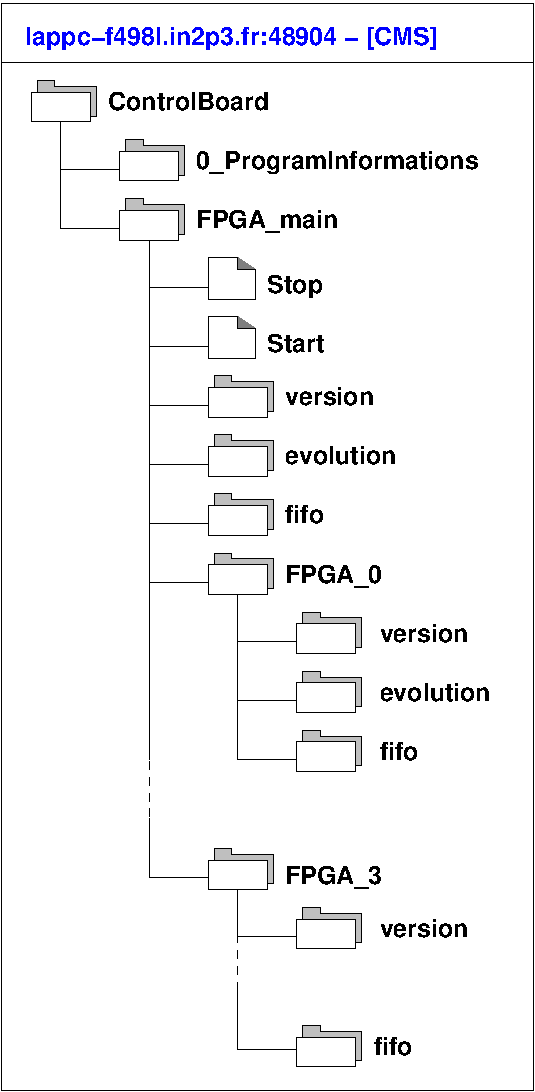
\includegraphics[width=5cm]{appendix/images/MOS_device_example_1.pdf}
\end{center}
\caption{Example of a  device managed through a MOS  server.  The root
  device is named \texttt{ControlBoard}.  First level daughter devices
  are  \texttt{0\_ProgramInformations} and  \texttt{FPGA\_main}.  Here
  the          MOS/OPCUA          server          is          labelled
  \texttt{CMS}.}\label{fig:an:mos_dev_1}
\end{figure}

% TODO


\subsection{Integration of a new device in the Vire environment}

The Vire  API also implements a  mechanism to describe a  hierarchy of
devices.  This  mechanism is independant  of the  one used in  the MOS
system but can  be easily made compatible with it.   This means that a
MOS  hierarchy  of devices  can  be  represented  in Vire.   The  Vire
hierarchy of  devices can  be considered as  some kind  of filesystem,
each device  being a folder with  its unique path, as  shown on figure
\ref{fig:an:mos_dev_2}.   The \emph{methods}  associated to  a devices
(or a datapoint) can be considered as plain executable files stored in
the  device's folder  : they  constitute the  set of  \emph{resources}
associated to the device.


\begin{figure}[h]
\begin{center}
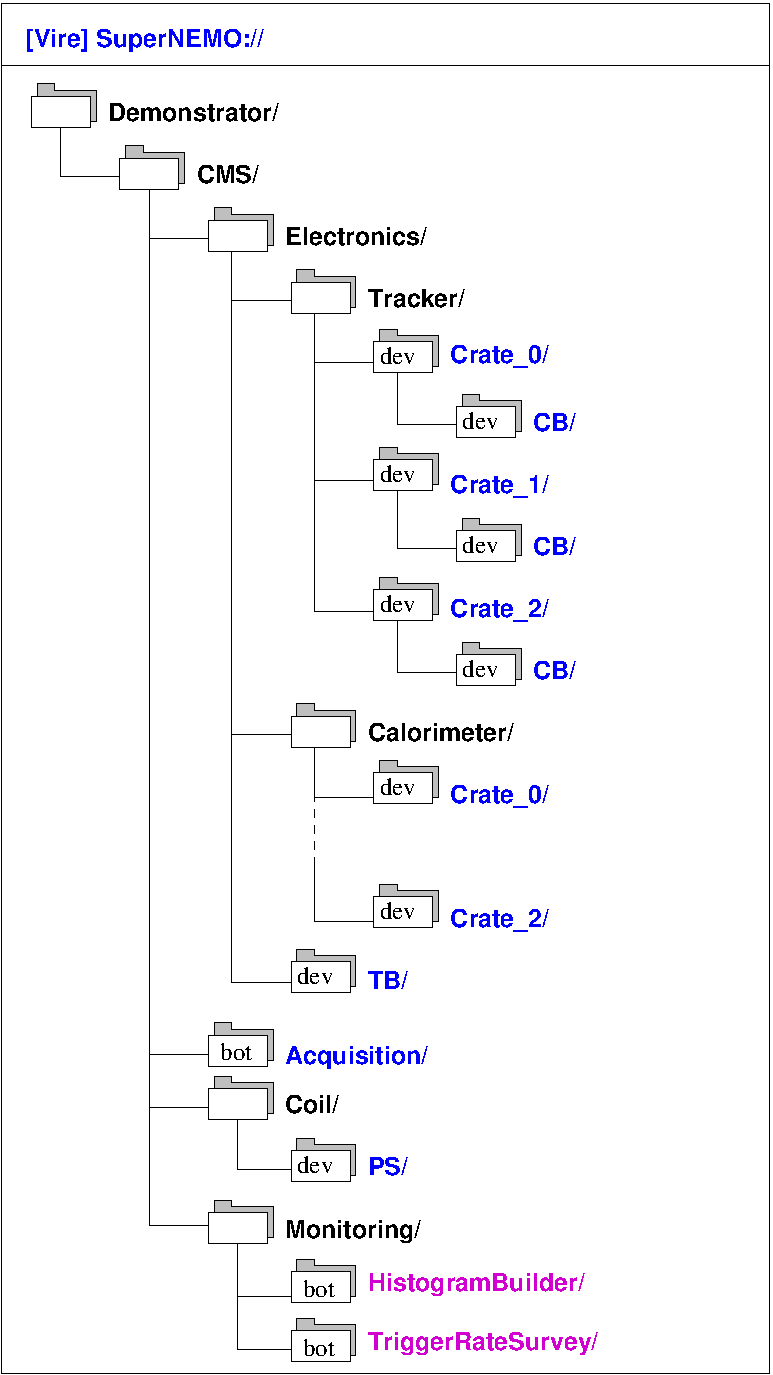
\includegraphics[width=5cm]{appendix/images/MOS_device_example_2.pdf}
\end{center}
\caption{Example of a hierarchy of  devices described by the Vire API.
  The root device is named  \texttt{SuperNEMO:}.  The top level (root)
  device  is  named  \texttt{Demonstrator}.  The  devices  colored  in
  \textcolor{blue}{blue}  are managed  through MOS/OPCUA.  The devices
  colored in \textcolor{magenta}{magenta} are directly embedded in the
  Vire server.  Devices with the \texttt{dev} tag are typical hardware
  device.  Devices  with the  \texttt{bot}  tag  are typical  software
  devices.   The  devices  colored in  \textbf{black}  are  structural
  pseudo-devices used to organize and  present a comprehensive view of
  the hierarchy. }\label{fig:an:mos_dev_2}
\end{figure}

The organisation of this hierarchy of devices is arbitrary and defined
by the designer of the  \emph{Control and Monitoring System}.  What is
important  to  understand  is  that  some  of  these  devices  can  be
associated  to  \emph{hardware  devices}  (a  power  supply  crate,  a
temperature probe\dots) and others  can be \emph{pseudo-devices}, i.e.
pure   software  object   (a   monitoring  robot,   a  file   transfer
daemon\dots).

In the context of the coupling of  the Vire server and the CMS server,
we are  in the event that  some devices are managed  by some MOS/OPCUA
servers and others are managed  in the Vire server itself.  Typically,
\emph{hardware devices}  are systematically managed through  the OPCUA
technology.  Vire has a mechanism to integrate such devices in its own
hierarchy.  This mechanism can  be considered like the \emph{mounting}
of   a   remote   filesystem   from  a   local   filesystem.    Figure
\ref{fig:an:mos_dev_0} illustrates  the case of many  hardware devices
-- managed by MOS -- that are integrated in the Vire system.  From the
Vire point of  view, the user does not see  the implementation details
for such  devices. He  does not  know the identity  of the  MOS server
hosting the device. He does not even know if the device is hosted by a
MOS server.  Devices are simply visible through the standard hierarchy
published by Vire with its  own device naming scheme, regardless their
true location.



\begin{figure}[h]
\begin{center}
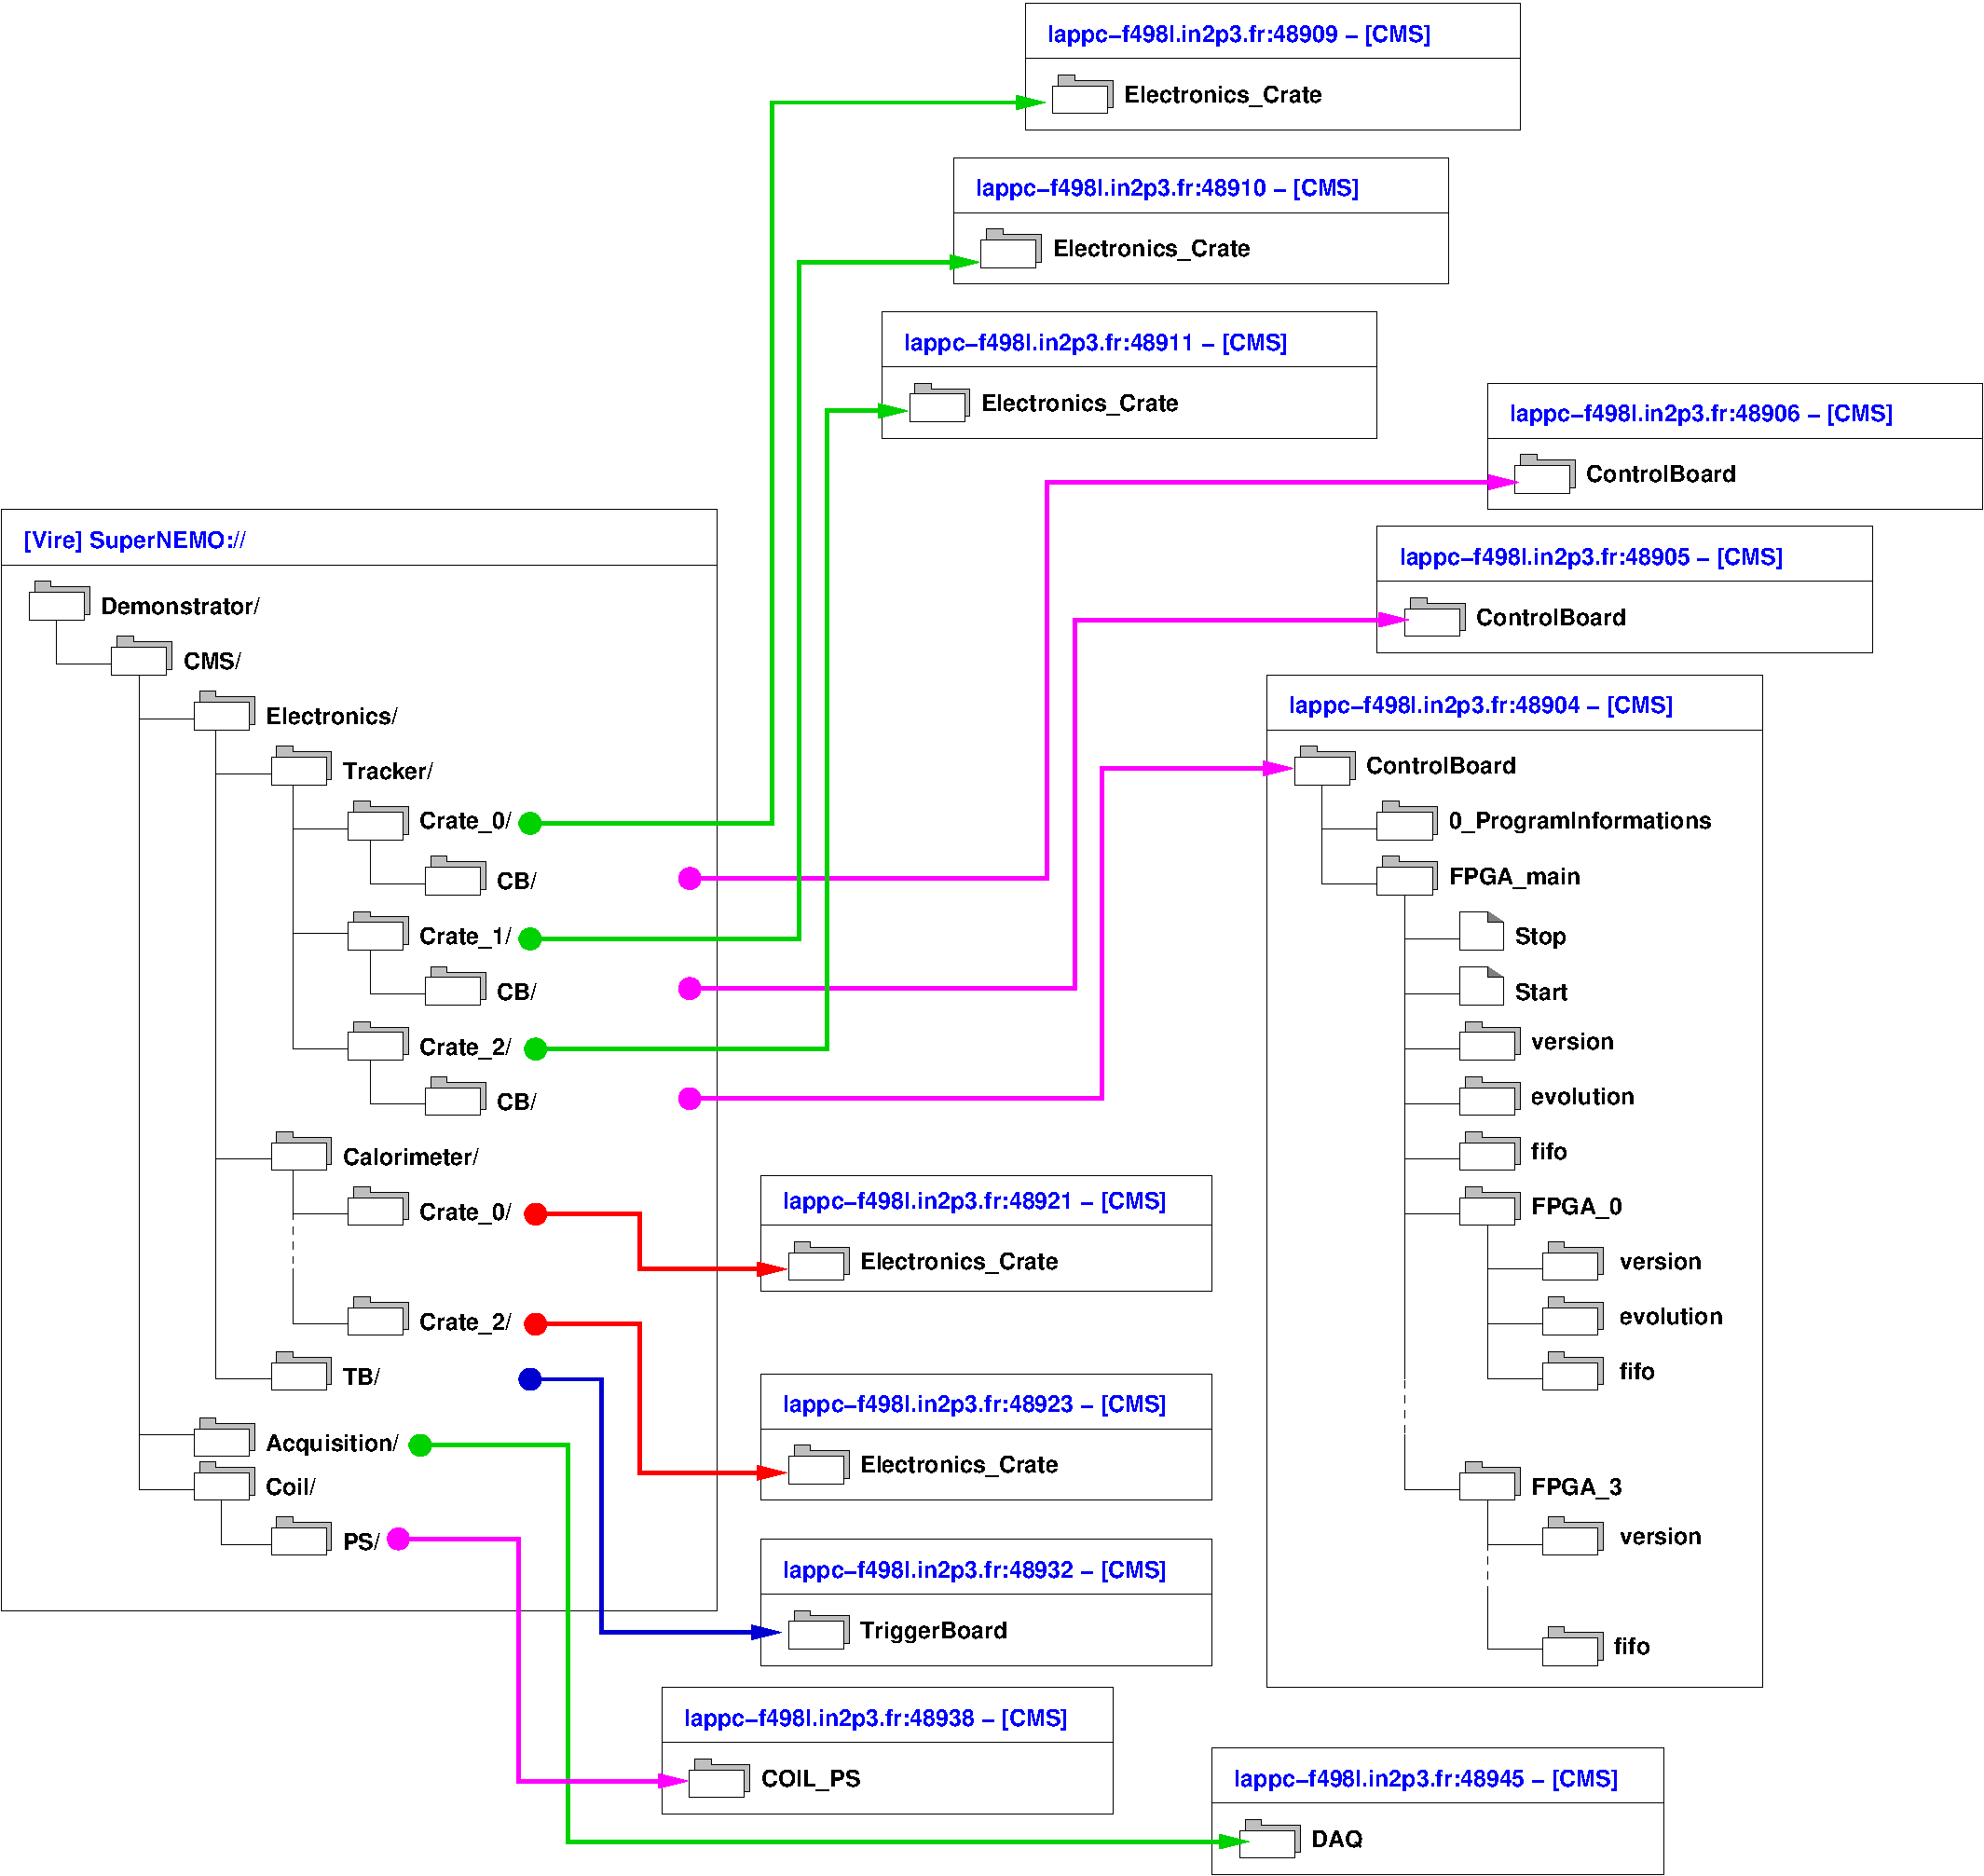
\includegraphics[width=\linewidth]{appendix/images/MOS_device_example_0.pdf}
\end{center}
\caption{The  mounting of  many  MOS device  hierarchies  in the  Vire
  device hierarchy.  Each OPCUA server  runs a simple  hardware device
  that is \emph{mounted} from a specific node with its own path.
%% of  devices described by the Vire API.
%%   The root device is named  \texttt{SuperNEMO:}.  The top level (root)
%%   device is  named \texttt{Demonstrator}. The devices  colored in blue
%%   are managed  through MOS/OPCUA. The  devices colored in  magenta are
%%   directly embedded in the Vire server.  Devices with the \texttt{dev}
%%   tag are typical  hardware device. Devices with  the \texttt{bot} tag
%%   are typical software devices.
}\label{fig:an:mos_dev_0}
\end{figure}




\subsection{Example}

Using  the examples  displayed  in  figure \ref{fig:an:mos_dev_0},  we
consider  in detail  the way  one specific  device managed  by MOS  is
mounted   in  the   Vire   hierarchy.  Figure   \ref{fig:an:mos_dev_3}
illustrates the mounting of a MOS device in Vire.

Here the Vire  server publishes the path of a  device representing the
control board  of the third  electronic crate  for the tracker  of the
SuperNEMO demonstrator module.  The full Vire path of this device is:

\textcolor{blue}{\texttt{SuperNEMO://Demonstrator/CMS/Electronics/Tracker/Crate\_2/CB}}

This is  the only Vire identifier  recognized by user to  address this
device.

On    the   figure,    one    can   see    that    the   MOS    server
\texttt{lappc−f498l.in2p3.fr} (port 48904) hosts a simple device which
is locally named \texttt{ControlBoard}.

When  mounting   this  device  in   the  Vire  hierarchy,   the  local
\texttt{[CMS]}  namespace and  \texttt{ControlBoard} device  names are
hidden and replaced by the Vire device path.  All daughter devices and
datapoints of  the \texttt{CMS/ControlBoard} device are  integrated as
daughters        of        the         Vire        device        named\\
\texttt{SuperNEMO://Demonstrator/CMS/Electronics/Tracker/Crate\_2/CB}.


For example, the \texttt{FPGA\_main} daughter device is now associated
to the following Vire path:

\textcolor{blue}{\texttt{SuperNEMO://Demonstrator/CMS/Electronics/Tracker/Crate\_2/CB/FPGA\_main/}}

and  its  \texttt{Stop} method  is  automatically  addressed with  the
following \emph{leaf} path:

\textcolor{blue}{\texttt{SuperNEMO://Demonstrator/CMS/Electronics/Tracker/Crate\_2/CB/FPGA\_main/Stop}}


\begin{figure}[h]
\begin{center}
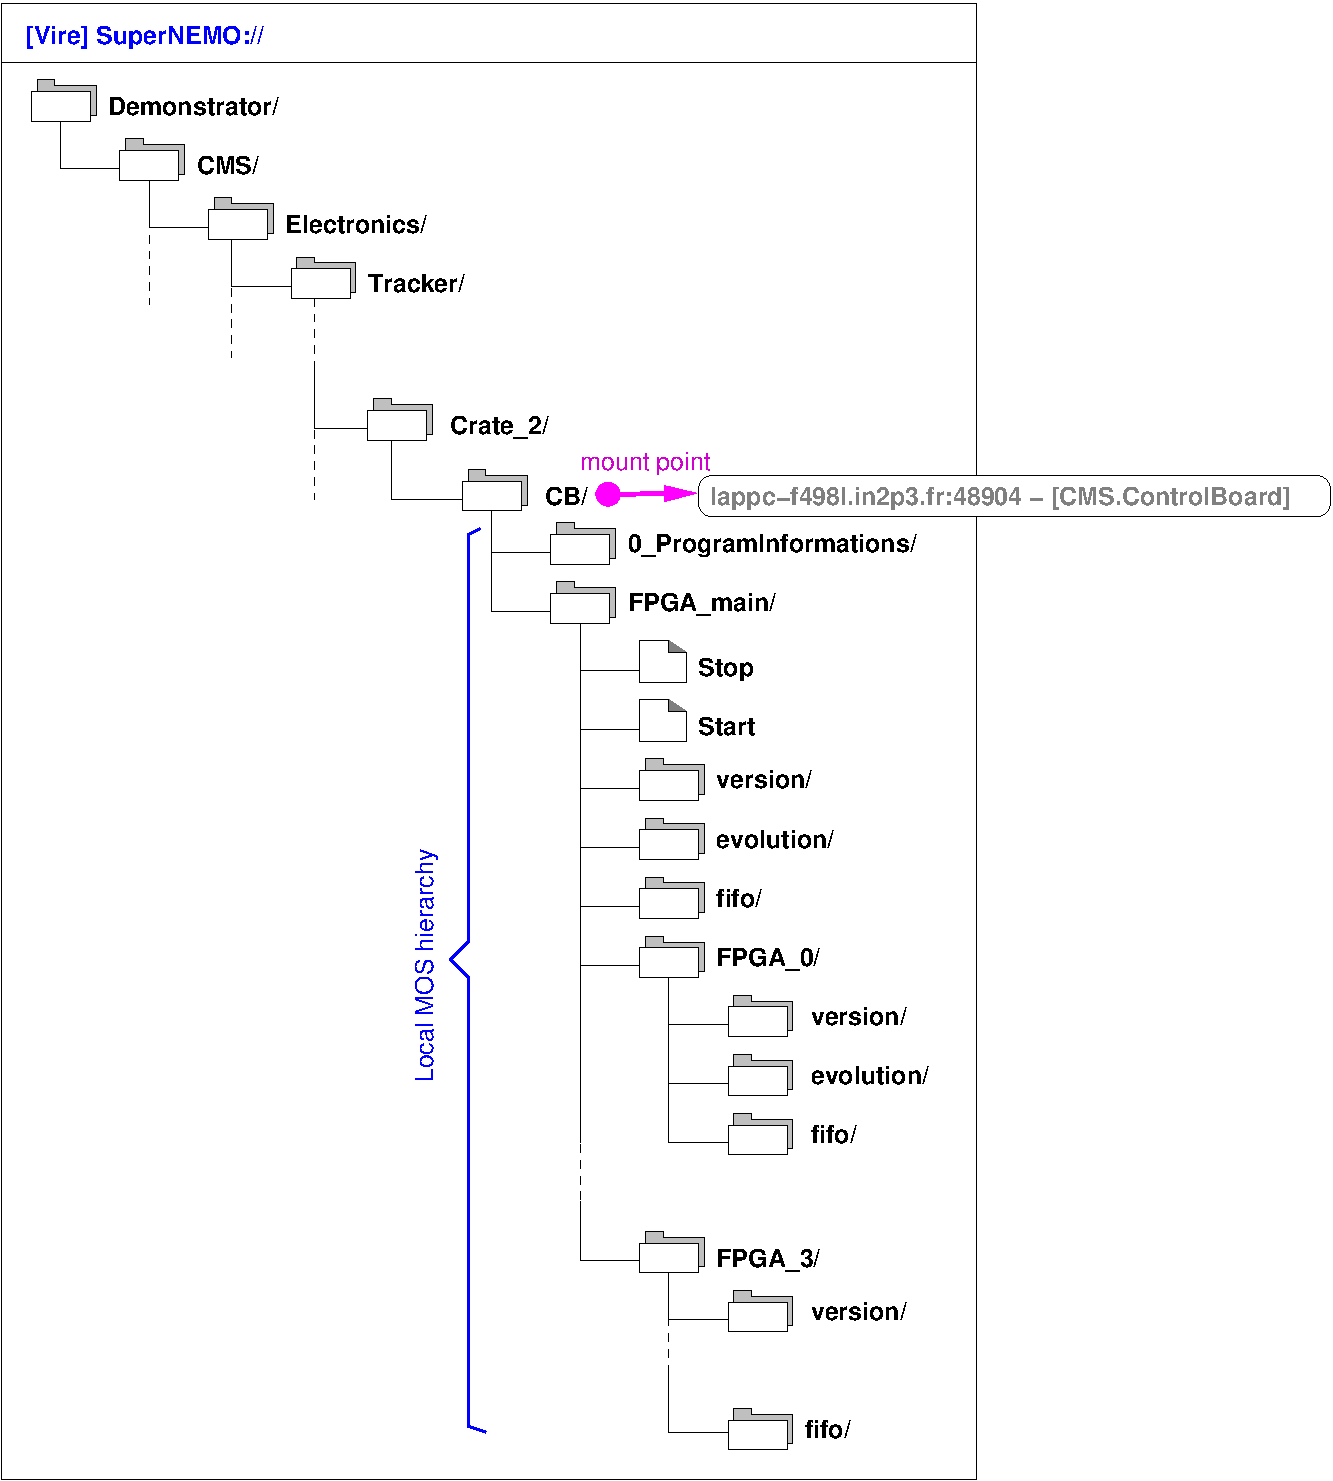
\includegraphics[width=0.8\linewidth]{appendix/images/MOS_device_example_3.pdf}
\end{center}
\caption{The  mounting of  one  MOS device and its local hierarchy  in the  Vire
  device hierarchy.}\label{fig:an:mos_dev_3}
\end{figure}



\subsection{Vire/MOS mapping}

As it can be  seen in the above example, the integration  of a new MOS
device in the Vire system is  achieved through soem kind of filesystem
mounting operation.   Particularly, it is  shown that the MOS  name of
the   mounted  root   device  is   replaced  by   an  arbitrary   Vire
path. However, all daughter  nodes (devices, datapoints) attached from
this root  node have their  relative MOS  names preserved in  the Vire
naming scheme.

Any  resource  (method)  associated  to any  of  such  daughter  nodes
inherits this relative naming scheme.

As Vire applications  describe resources through their  Vire paths, it
is thus needed to build an explicit map that associates resource paths
to MOS address  and name. The CMS  server will be able  to resolve the
MOS server/port and  embedded device associated to  the resource path.

The goal of the \texttt{devices\_launch.conf} file is not only to tell
the CMS server what MOS server should  be loaded and ran at start, but
also  to describe  the  \emph{mounting point/names}  used  by Vire  to
access the resources associated to MOS devices.  From the informations
stored in the  file, an explicit associative array must  be built when
the Vire server connect to the CMS server.  It will play the role of a
resource path resolver  when requests about resources will  be sent by
Vire applications.  This associative array  must be locked  during the
Vire/CMS connection.



%\subsubsection{Preparation of XML device models}

%% \noindent\underline{Pre-condition:}
%% The device is working and validated through the MOS/OPCUA server

%% \begin{enumerate}

%% \item Produce XML décrivant le modèle du device enrichi
%%   des metadata
%% Rédaction du fichier XML décrivant le modèle du device

%% \item Génération des fichiers model du type de device pour Vire

%% \item Génération des fichiers instances resolv.conf

%% \end{enumerate}


\vfill
\pagebreak
\clearpage

% end


\section{Vire messages}\label{app:vire_messages}

Within Vire  and between Vire  components and external  components, we
use  a communication  system  based on  Vire  messages.  This  section
describes the structure of such messages.

\subsection{General structure of a message}

Each message consists in two parts (figure \ref{fig-vire-message-message-cpp}):
\begin{itemize}

\item  the  \emph{header}  is   dedicated  to  generic  and  typicalle
  mandatory  informations  which  document   the  message  itself  and
  arbitrary high-level metadata.

\item  the \emph{body}  of the  message  contains the  real data: the payload.
  The structure of the message body depends on some convention. Vire uses
  its own convention to embed the payload data.

\end{itemize}

\begin{figure}[h]
\vskip 10pt
\small
\begin{Verbatim}[frame=single,xleftmargin=0.cm,label=\fbox{C++}]
struct vire::message::message {
  message_header header; // Header of the message
  message_body   body;   // Body of the message
};
\end{Verbatim}
\normalsize
\caption{The structure of a Vire message object (C++  class:
  \texttt{"vire::message::message"})}\label{fig-vire-message-message-cpp}
\end{figure}

\subsection{The message header}

The header contains (figure \ref{fig-vire-message-message_header-cpp}):
\begin{itemize}

  \item The mandatory \texttt{message\_id}  attribute is an identifier
    of the  message which  document the emitter  and a  unique message
    number.   Each emitter  is  responsible of  the  numbering of  the
    messages it  emits, typically using an  incremental technique. The
    message  number is  a positive  integer, starting  from 0  (figure
    \ref{fig-vire-message-message_identifier-cpp}).

  \item  The \texttt{timestamp}  attribute  encodes the  approximative
    time point when the message was  created. It contains the date and
    the time, using at least microsecond resolution.

    Typically,  with  JSON  encoding  system, it  is  expected  to  be
    formatted as a character string, using the following ISO format:

    \begin{center}
      \texttt{yyyymmddThhmmss.uuuuuu}
    \end{center}

    \noindent where:

    \vskip -10pt
    \begin{itemize}
    \item[\texttt{yyyymmdd} :] encodes year/month/day,
    \item[\texttt{hhmmssd} :] encodes hour/minute/second,
    \item[\texttt{uuuuuu} :] encodes microseconds.
    \end{itemize}

  \item   In   the   case    of   a   \emph{response}   message,   the
    \texttt{in\_reply\_to} attribute is set to identify the associated
    request message.

  \item  The \texttt{asynchronous}  boolean  attribute is  set if  the
    message processing  is explicitely requested  by the source  to be
    asynchronous (non-blocking).  In  RPC transactions, where requests
    are transmitted from one point to  the other, its default value is
    \emph{false}.   It  is possible  to  force  a RPC  transaction  in
    asynchronous mode.   This use  case is documented  elsewhere.  For
    event messaging, this flag is conventionally set to \emph{true}.

  \item  The  \texttt{body\_layout\_id}  attribute  is  the  mandatory
    identifier   of   the   layout   of  the   message   body   (class
    \texttt{"vire::utility::model\_identifier"}).  The  default layout
    for     message     body     inside    the     Vire     API     is
    \texttt{"vire::message::body\_format::typed\_payload"}, with version
    \texttt{"1.0"}                                             (figure
    \ref{fig-vire-utility-model_identifier-cpp}).

\end{itemize}


\begin{figure}[h]
\vskip 10pt
\small
\begin{Verbatim}[frame=single,xleftmargin=0.cm,label=\fbox{C++}]
struct vire::message::message_header {
  message_identifier message_id;     // Message identifier from the emitter.
  std::string        timestamp;      // Timestamp.
  message_identifier in_reply_to;    // Message identifier of the associated
                                     // request message (optional).
  bool               asynchronous,   // Asynchronous flag.
  vire::utility::model_identifier     body_layout_id; // Body layout identifier.
  std::map<std::string, std::string>  metadata;       // Key/value metadata dictionary.
};
\end{Verbatim}
\normalsize
\caption{The  structure  of  a   message  header  object  (C++  class:
  \texttt{"vire::message::message\_header"}).}\label{fig-vire-message-message_header-cpp}
\end{figure}

\begin{figure}[h]
\vskip 10pt
\small
\begin{Verbatim}[frame=single,xleftmargin=0.cm,label=\fbox{C++}]
struct vire::message::message_identifier {
  std::string emitter; // Name identifying the emitter of the message.
  int32_t     number;  // Number identifying the message in the emitter's
                       // message numbering scheme.
};
\end{Verbatim}
\normalsize
\caption{The      structure      of     a      message      identifier
  (C++  class:  \texttt{"vire::message::message\_identifier"}).}
\label{fig-vire-message-message_identifier-cpp}
\end{figure}

\begin{figure}[h]
\vskip 10pt
\small
\begin{Verbatim}[frame=single,xleftmargin=0.cm,label=\fbox{C++}]
struct vire::utility::model_identifier {
  std::string name;    // Name identifying the format of the message.
  std::string version; // String identifying the version of the format.
};
\end{Verbatim}
\normalsize
\caption{The structure of a model identifier (C++  class:  \texttt{"vire::utility::model\_identifier"}.}\label{fig-vire-utility-model_identifier-cpp}
\end{figure}




\begin{figure}[h]
\vskip 10pt
\small
\begin{Verbatim}[frame=single,xleftmargin=0.cm,label=\fbox{JSON}]
{
   "header" : {
      "message_id" : {
         "emitter" : "vire.server",
         "number" : 42
      },
      "timestamp" : "20160930T141408.413443",
      "in_reply_to" : {
         "initialized" : true,
         "value" : {
            "emitter" : "vire.client.0",
            "number" : 23
         }
      },
      "asynchronous" : false,
      "body_layout_id" : {
         "name" : "vire::message::body_format::typed_payload",
         "version" : {
            "initialized" : true,
            "value" : "1.0"
         }
      },
      "metadata" : [
         {
            "key" : "key1",
            "value" : "foo"
         },
         {
            "key" : "key2",
            "value" : "42"
         },
         {
            "key" : "key3",
            "value" : "3.1415899999999999"
         },
         {
            "key" : "key4",
            "value" : "true"
         }
      ]
   }
  "body" : {
      ...
   }
}
\end{Verbatim}
\normalsize
\caption{Example of  a   message  header  object in JSON format.}
\label{fig-vire-message-message_header-json}
\end{figure}

\vfill
\clearpage
\pagebreak

\subsection{The message body}

The    default    message   body    layout    in    Vire   is    named
\texttt{"vire::message::body\_format::typed\_payload"}        (version
\texttt{"1.0"}).   Each  message used  within  the  Vire framework  is
supposed to use this layout.  The general idea is that the body of the
message embeded the  \emph{payload object} that has  to be transmitted
between  two components  of  the system.   \emph{Payload objects}  are
classified in one of the three following categories:

\begin{enumerate}

\item \emph{Request}:  describes a request submitted  by one component
  to another component (generally during a synchronous RPC transaction).

\item  \emph{Response}: describes  the  response to  a former  request
  (generally during a synchronous RPC transaction).

\item \emph{Event}: describes an  arbitrary information record (alarm,
  exception, signal\dots) which is transmitted asynchronously.

\end{enumerate}

Vire implements the following class hierarchy:

\begin{center}
\begin{tikzpicture}
  \node (payload)  at (0,2)  [draw] {\texttt{vire::utility::base\_payload}};
  \node (request)  at (-4,0) [draw] {\texttt{vire::utility::base\_request}};
  \node (response) at (2,0)  [draw] {\texttt{vire::utility::base\_response}};
  \node (event)    at (8,0)  [draw] {\texttt{vire::utility::base\_event}};

  %\draw[style=help lines] (-3,-1) grid (10,4);
  \draw (node cs:name=response,anchor=north) |- (0,1);
  \draw (node cs:name=event,anchor=north)    |- (0,1);
  \draw[->] (node cs:name=request,anchor=north)
  |- (0,1) -| (node cs:name=payload,anchor=south);
\end{tikzpicture}
\end{center}

The requirements for the transmitted object are the following:

\begin{itemize}

\item The  type of the object  must be conventionally associated  to a
  unique     \emph{model      identifier}     object      (see     the
  \texttt{"vire::utility::model\_identifier"} class)  which contains a
  unique   name   (\textit{string    identifier})   and   possibly   a
  \textit{version identifier}.  Each software  component that may send
  or  receive the  object  should agree  on  this type  identification
  scheme.   This   enable  the  use  of   object  factories,  whatever
  programming  langage  is used  on  both  side of  the  communication
  system.

\item  For each  software component,  the object  type must  have some
  dedicated  encoding/decoding  functions  available  (again  whatever
  programming language is used). For example the Vire API supports the
  following encoding formats:

  \begin{itemize}

  \item JSON (MIME  encoding type: \texttt{"application/x-json"}), which
    is supportable by many languages,

  \item  Protobuf  (Google  Protocol   Buffers,  MIME  encoding  type:
    \texttt{"application/x-protobuf"}), which is also widely supported,

  \item   Boost/serialisation   (XML,    text   or   binary   archives
    \texttt{"application/x-boost-serialization-xml"},
    \texttt{"application/x-boost-serialization-text"},
    \texttt{"application/x-boost-serialization-binary"}),    which    in
    principle is supported by C++ only.

  \end{itemize}

  The Protobuf  encoding format will be  used to serialize/deserialize
  the  Vire  messages transported  between  the  Vire server  and  the
  CMS/LAPP server.

\end{itemize}

Vire uses a dedicated layout to represent the body of any message with
its embedded payload object. With this technique, the structure of the
body          contains         two          attributes         (figure
\ref{fig-app-vire-message-message_body-cpp}):

\begin{enumerate}

\item The \texttt{payload\_type\_id} specifies the type of the payload
  object   (figure   \ref{fig-app-vire-utility-model_identifier-cpp}).
  This unique name  is conventionaly fixed for a  given application. A
  version tag allows to support possible evolution of the object type.

\item The  \texttt{payload} is a  handle to  a payload object  of type
  request, response or event.

  %% \begin{itemize}
  %% \item Within  the producer  component of  the message,  the encoding
  %%   function associated to the object  type is responsible to generate
  %%   the JSON stream for the object and store it in the buffer.

  %% \item Within  the consumer  component of  the message,  the decoding
  %%   function associated to the object type is responsible to parse the
  %%   JSON stream stored in the buffer and restore the object in memory.

  %% \end{itemize}

  It is expected  that, on both sides of the  connection, the software
  components can  access dedicated  software plugins which  ensure the
  support  of  various   \emph{payload  object  types}  conventionnaly
  associated  with  their  \emph{payload type  identifiers}  and  also
  providing JSON and/or Protobuf encoding/decoding functionalities.

  %% The   system  allows  to  support
  %% modification  in the  structure of  the objects  thanks to  version
  %% tagging.

\end{enumerate}

\begin{figure}[h]
\vskip 10pt
\small
\begin{Verbatim}[frame=single,xleftmargin=0.cm,label=\fbox{C++}]
struct message_body {
  vire::utility::model_identifier     payload_type_id; // Object type identifier.
  const vire::utility::base_payload * payload;         // Handle to a payload object.
};
\end{Verbatim}
\normalsize
\caption{The structure of a message body object (C++).}
\label{fig-app-vire-message-message_body-cpp}
\end{figure}

\begin{figure}[h]
\vskip 10pt
\small
\begin{Verbatim}[frame=single,xleftmargin=0.cm,label=\fbox{JSON}]
{
  "header" : {
    ...
  },
  "body" : {
    "payload_type_id" : {
      "name" : "vire::message::testing::error_event",
      "version" : {
        "initialized" : false
      }
    },
    "payload" : {
      "timestamp" : "20160930T141743.759085"
      "err" : {
        "code" : 3,
        "message" : "A basic error"
      },
    }
  }
}
\end{Verbatim}
\normalsize
\caption{Example of  a   message  body  object in JSON format.}
\label{fig-vire-message-message_body-json}
\end{figure}

\vfill
\clearpage
\pagebreak

% end

%\input{appendix/app_json_fmt.tex}

\section{The \emph{Protocol Buffers} format}\label{app:protobuf_fmt}

\subsection{Introduction}

The  Google  Protocol Buffers  (\emph{protobuf})  library  is used  to
represent the objects that are exchanged between the Vire clients, the
Vire server and the CMS server.  The  version 3 of the format is used,
implying   at   least   version   3.0.0  (September   2016)   of   the
\emph{protobuf} library.

Each  data   structure  of  interest   can  be  described   through  a
\texttt{.proto}  file  from  which  stub files  can  be  automatically
generated  with the  \texttt{protoc} compiler.  For Vire  and its  CMS
interface, the C++ and Java programming languages will be used.


A  collection of  \texttt{.proto}  files are  provided  with the  Vire
library to represent all kind  of data structures transferable between
networked agents  (Vire server,  Vire clients, CMS/LAPP  server).  The
objects of  the highest level  are named \emph{payload  objects} (like
\emph{request},  \emph{response} and  \emph{event} objects).   They
are composed of attributes of more basic data structures.

\subsection{Example}

The following  class diagram  illustrates two data  structures defined
within the Vire library with an inheritance relationship between them.

\begin{center}
  \begin{tikzpicture}
    \node (base)     at (0,1.5)  [draw] {\texttt{vire::utility::base\_error}};
    \node (setup)    at (0,0)  [draw] {\texttt{vire::utility::invalid\_setup\_id\_error}};

    \draw[->]   (node cs:name=setup,anchor=north) |- (0,1);
    |- (0,1) -| (node cs:name=base,anchor=south);
  \end{tikzpicture}
\end{center}

The \texttt{vire::utility::base\_error}  is the  parent class  for all
\emph{error}  objects.   It  contains   two  attributes:   an  integer
\emph{error code}  and a  character string describing  the \emph{error
  message}.

The   \texttt{vire::utility::invalid\_setup\_id\_error}  class   is  a
specialized error class  which represents explicitely an  error due to
an identification  failure of  the experimental setup.   It implements
additional mutually exclusive attributes: the \emph{unrecognized name}
of the setup or the \emph{unrecognized version} of the setup.

This   example  illustrates   the  protobuf   representation  of   the
\texttt{vire::utility::base\_error}  in the  Vire  library, using  the
\texttt{"vire/utility/BaseError.proto"} file:

\small
\begin{Verbatim}[frame=single,xleftmargin=0.cm,label=\fbox{protobuf}]
  syntax = "proto3";
  package vire.utility; // Namespace

  message BaseError {

    // reserved 1; // Reserved for _base message

    // Attributes:
    int32  code           = 100; // The error code
    string message_format = 101; // The error description message

  }
\end{Verbatim}
\normalsize

\vfill
\clearpage
\pagebreak

\subsection{Vire protobuf conventions}

Vire uses the following conventions:

\begin{enumerate}

\item
  The member index  \texttt{1} is reserved to represent the  link of a
  class to its main base/parent class (if any).  It is not used if the
  data structure does not inherit any data structure.
  If a data structure naturally inherits another one, it is thus possible
  to  represent the  inheritance  relationship as  illustrated with  the
  \texttt{"vire/utility/InvalidSetupIdError.proto"}      file      which
  represents the \texttt{vire::utility::invalid\_setup\_id\_error} class
  in the Vire library:

  \small
  \begin{Verbatim}[frame=single,xleftmargin=0.cm,label=\fbox{protobuf}]
    syntax = "proto3";
    package vire.utility; // Namespace

    import "vire/utility/BaseError.proto"; // Dependency

    message InvalidSetupIdError {

      BaseError _base = 1; // The base class

      // Additional attributes:
      oneof detail { // Mutual exclusion
        string invalid_setup_name    = 100; // The failed setup name
        string invalid_setup_version = 101; // The failed setup version
      }

    }
  \end{Verbatim}
  \normalsize

\item The  \texttt{\_base} member  is conventionally  used to  represent the
  inheritance   relationship    from   a   data   structure    of   type
  \texttt{"vire.utility.BaseError"}.

\item Member indexes from \texttt{2}  to \texttt{99} are also reserved
  for possible future usage (multiple inheritance, metadata\dots).

\item
  The first member of the data structure must start at index \texttt{100}.

\end{enumerate}

\vfill
\clearpage
\pagebreak

% end


\section{Vire payload objects}\label{app:payload}

\subsection{Introduction}

As  mentioned in  appendix \ref{app:protobuf_fmt},  Vire messages  are
wrappers for \emph{payload objects}.  Each  type of payload object can
be represented  through the \emph{protobuf} mechanism.   The following
class hierarchy shows the base architecture used to define new payload
objects.

\begin{center}
\begin{tikzpicture}
  \node (payload)  at (0,2)   [draw] {\texttt{vire::utility::base\_payload}};
  \node (request)  at (-4,0)  [draw] {\texttt{vire::utility::base\_request}};
  \node (response) at (2,0)   [draw] {\texttt{vire::utility::base\_response}};
  \node (event)    at (8,0)   [draw] {\texttt{vire::utility::base\_event}};
  \node (my)       at (-4,-2) [draw] {\texttt{my\_request}};
  \node (your)     at (2,-2)  [draw] {\texttt{your\_response}};
  \node (its)    at (8,-2)    [draw] {\texttt{its\_alarm}};

  %\draw[style=help lines] (-6,-2) grid (10,2);
  \draw (node cs:name=response,anchor=north) |- (0,1);
  \draw (node cs:name=event,anchor=north)    |- (0,1);
  \draw[->] (node cs:name=request,anchor=north)
  |- (0,1) -| (node cs:name=payload,anchor=south);
  \draw[->] (node cs:name=my,anchor=north)
  |- (-4,-1) -| (node cs:name=request,anchor=south);
  \draw[->] (node cs:name=your,anchor=north)
  |- (2,-1) -| (node cs:name=response,anchor=south);
  \draw[->] (node cs:name=its,anchor=north)
  |- (8,-1) -| (node cs:name=event,anchor=south);
\end{tikzpicture}
\end{center}


\begin{center}
\vskip 10pt
\small
\begin{tabular}{|l|l|l|}
  \hline
  \textbf{Vire C++ class} & \textbf{protobuf message type} & \textbf{protobuf definition file} \\
  \hline
  \hline
  \multicolumn{3}{|c|}{\emph{general types}} \\
  \hline
  boost::posix\_time::ptime & google.protobuf.Timestamp & google/protobuf/timestamp.proto \\
  \hline
  \hline
  \multicolumn{3}{|c|}{\emph{identifier types}} \\
  \hline
  vire::utility::base\_identifier & vire.utility.Baseidentifier & vire/utility/Baseidentifier.proto \\
  \hline
  vire::utility::instance\_identifier & vire.utility.InstanceIdentifier & vire/utility/InstanceIdentifier.proto \\
  \hline
  vire::utility::model\_identifier & vire.utility.ModelIdentifier & vire/utility/ModelIdentifier.proto \\
  \hline
  \hline
  \multicolumn{3}{|c|}{\emph{error types}} \\
  \hline
  vire::utility::base\_error & vire.utility.BaseError & vire/utility/BaseError.proto \\
  \hline
  vire::utility::invalid\_context\_error & vire.utility.InvalidContextError & vire/utility/InvalidContextError.proto \\
  \hline
  vire::utility::invalid\_setup\_id\_error & vire.utility.InvalidSetupIdError & vire/utility/InvalidSetupIdError.proto \\
  \hline
  \hline
  \multicolumn{3}{|c|}{\emph{payload types}} \\
  \hline
  vire::utility::base\_payload & vire.utility.BasePayload & vire/utility/BasePayload.proto \\
  \hline
  vire::utility::base\_request & vire.utility.BaseRequest & vire/utility/BaseRequest.proto \\
  \hline
  vire::utility::base\_response & vire.utility.BaseResponse & vire/utility/BaseResponse.proto \\
  \hline
  vire::utility::base\_event & vire.utility.BaseEvent & vire/utility/BaseEvent.proto \\
  \hline
  vire::utility::base\_alarm & vire.utility.BaseAlarm & vire/utility/BaseAlarm.proto \\
  \hline
  \hline
  \multicolumn{3}{|c|}{\emph{messenging types}} \\
  \hline
  vire::message::message\_identifier & vire.message.MessageIdentifier & vire/message/MessageIdentifier.proto \\
  \hline
  vire::message::msg\_header & vire.message.MsgHeader & vire/message/MsgHeader.proto \\
  \hline
  vire::message::msg\_body & vire.message.MsgBody & vire/message/MsgBody.proto \\
  \hline
  vire::message::message & vire.message.Message & vire/message/Message.proto \\
  \hline
\end{tabular}
\normalsize
\end{center}


\begin{center}
\vskip 10pt
\small
\begin{tabular}{|l|l|l|}
  \hline
  \multicolumn{3}{|c|}{\emph{Resource management related types}} \\
  \hline
  vire::cms::resource\_status\_record & vire.cms.ResourceStatusRecord & vire/cms/ResourceStatusRecord.proto \\
  \hline
  vire::cms::resource\_fetch\_status\_request & vire.cms.ResourceFetchStatusRequest & vire/cms/ResourceFetchStatusRequest.proto \\
  \hline
  vire::cms::resource\_fetch\_status\_success\_response & vire.cms.ResourceFetchStatusSuccessResponse & vire/cms/ResourceFetchStatusSuccessResponse.proto \\
  \hline
  vire::cms::resource\_fetch\_status\_failure\_response & vire.cms.ResourceFetchStatusFailureResponse & vire/cms/ResourceFetchStatusFailureResponse.proto \\
  \hline
  vire::cms::resource\_exec\_request & vire.cms.ResourceExecRequest & vire/cms/ResourceExecRequest.proto \\
  \hline
  vire::cms::resource\_exec\_success\_response & vire.cms.ResourceExecSuccessResponse & vire/cms/ResourceExecSuccessResponse.proto \\
  \hline
  vire::cms::resource\_exec\_failure\_response & vire.cms.ResourceExecFailureResponse & vire/cms/ResourceExecFailureResponse.proto \\
  \hline
  vire::cms::resource\_exec\_non\_blocking\_request & vire.cms.ResourceExecNonBlockingRequest & vire/cms/ResourceExecNonBlockingRequest.proto \\
  \hline
  vire::cms::resource\_exec\_non\_blocking\_ack\_response & vire.cms.ResourceExecNonBlockingAckResponse & vire/cms/ResourceExecNonBlockingAckResponse.proto \\
  \hline
  vire::cms::resource\_exec\_non\_blocking\_noack\_response & vire.cms.ResourceExecNonBlockingNoackResponse & vire/cms/ResourceExecNonBlockingNoackResponse.proto \\
  \hline
  vire::cms::resource\_exec\_non\_blocking\_success\_event & vire.cms.ResourceExecNonBlockingSuccessEvent & vire/cms/ResourceExecNonBlockingSuccessEvent.proto \\
  \hline
  vire::cms::resource\_exec\_non\_blocking\_failure\_event & vire.cms.ResourceExecNonBlockingFailureEvent & vire/cms/ResourceExecNonBlockingFailureEvent.proto \\
  \hline
  vire::cms::resource\_exec\_error & vire.cms.ResourceExecError & vire/cms/ResourceExecError.proto \\
  \hline
  vire::cms::invalid\_status\_error & vire.cms.ResourceExecError & vire/cms/ResourceExecError.proto \\
  \hline
  %% vire::cms::invalid\_credentials\_error & vire.cms.InvalidCredentialsError & vire/cms/InvalidCredentialsError.proto \\
  %% \hline
  %% vire::cms::invalid\_user\_error & vire.cms.InvalidUserError & vire/cms/InvalidUserError.proto \\
  %% \hline
  vire::cms::invalid\_resource\_error & vire.cms.InvalidUserError & vire/cms/InvalidUserError.proto \\
  \hline
  vire::cms::no\_pubsub\_resource\_error & vire.cms.NoPubsubResourceError & vire/cms/NoPubsubResourceError.proto \\
  \hline
  \hline
  \multicolumn{3}{|c|}{\emph{Resource pub/sub management types}} \\
  \hline
  vire::cms::resource\_pubsub\_subscribe\_request & vire.cms.ResourcePubsubSubscribeRequest & vire/cms/ResourcePubsubSubscribeRequest.proto \\
  \hline
  vire::cms::resource\_pubsub\_subscribe\_success\_response & vire.cms.ResourcePubsubSubscribeRSuccessResponse & vire/cms/ResourcePubsubSubscribeRSuccessResponse.proto \\
  \hline
  vire::cms::resource\_pubsub\_subscribe\_failure\_response & vire.cms.ResourcePubsubSubscribeRFailureResponse & vire/cms/ResourcePubsubSubscribeRSuccessResponse.proto \\
  \hline
  \hline
  \multicolumn{3}{|c|}{\emph{Vire/CMS server interface types}} \\
  \hline
  vire::cmsinterface::connection\_request & vire.cmsinterface.ConnectionRequest & vire/cmsinterface/ConnectionRequest.proto \\
  \hline
  vire::cmsinterface::connection\_success\_response & vire.cmsinterface.ConnectionSuccessResponse & vire/cmsinterface/ConnectionSuccessResponse.proto \\
  \hline
  vire::cmsinterface::connection\_failure\_response & vire.cmsinterface.ConnectionFailureResponse & vire/cmsinterface/ConnectionFailureResponse.proto \\
  \emph{embedded:} unknown\_resources\_error & .UnknownResourcesError &  \\
  \hline
  vire::cmsinterface::disconnection\_request & vire.cmsinterface.DisconnectionRequest & vire/cmsinterface/DisconnectionRequest.proto \\
  \hline
  vire::cmsinterface::disconnection\_success\_response & vire.cmsinterface.DisconnectionSuccessResponse & vire/cmsinterface/DisconnectionSuccessResponse.proto \\
  \hline
  %% \hline
  %% vire::cmsinterface::disconnection\_failure\_response & vire.cmsinterface.DisconnectionFailureResponse & vire/cmsinterface/DisconnectionFailureResponse.proto \\
\end{tabular}
\normalsize
\end{center}

\subsection{Basic data structures}

Any  payload object  (request, response  or event)  generally contains
some information records which are  specific to the functionalities of
the  payload  object they  belong.   These  records are  of  arbitrary
types. Of course they should be  translatable in terms of the protobuf
library.
%Of course they can be (de)serialized using JSON.
Some of these types are very  general and defined within the Vire core
API itself because they are reused by various payload objects not only
through  the Vire-CMS/LAPP  interface  but also  between  Vire clients  and
servers, independently  of the  CMS/LAPP server.  However,  the use  of the
Protocol Buffers interface makes possible  to publish the interface of
such data to the outside world, including the CMS/LAPP server in priority.

%% Other one are specific to the Vire/CMS interface and thus managed only
%% in the \texttt{Vire\_CMSInterface} API.
These  types  are considered  as  \emph{basic}.  Among them  we  find:
generic error  types, generic  identifier types,  timestamps, resource
status records\dots We propose to describe them in this section.

Once a sufficient collection of  basic data record types is available,
it  is possible  to describe  high  level payload  object types  which
aggregate attributes of such types.

Other record  types are specific to  some payload objects and  will be
never  used outside  the scope  of these  payload objects.   Such data
structures will be  explicitely declared with the  payload object they
belong to, likely as embedded types/classes.


\subsubsection{Errors}

Some  \emph{response} or  \emph{event} payload  objects may  contain a
specific  error  record  object.   A  \emph{failure  response}  or  an
\emph{exception  event}  object will  generally  embed  such an  error
record object.

Each  \emph{error record}  is represented  by an  instance of  a given
error type.   Each of  the error  types defined  in Vire  inherits the
\texttt{vire::utility::base\_error}      base       class      (figure
\ref{fig-app-payload-base_error})   which   contains   the   following
attributes:

\begin{itemize}

\item the error code: A non zero  integer which is set to 1 by default
  (indicating  a  generic  failure  case).   The  error  code  can  be
  conventionally  set to  any positive  integer value  to represent  a
  specific error case, depending on the context.

\item the error  message: an optional human  readable character string
  which documents the error as usefully as possible.

\end{itemize}

\begin{figure}[h]
\vskip 10pt
\small
\begin{Verbatim}[frame=single,xleftmargin=0.cm,label=\fbox{C++}]
struct vire::utility::base_error
{
  // Attributes:
  int         code;           // Error code (>0).
  std::string message_format; // Error message (optional).
};
\end{Verbatim}
\normalsize
\caption{The structure of a \texttt{"vire::utility::base\_error"} object
  (C++).}
\label{fig-app-payload-base_error}
\end{figure}


%% An example of JSON formatted basic error object is given in figure
%% \ref{fig-app-payload-base_error-1}.
%%
%% \begin{figure}[h]
%% \vskip 10pt
%% \small
%% \begin{Verbatim}[frame=single,xleftmargin=0.cm,label=\fbox{\texttt{JSON}}]
%% {
%%   "code" : "42",
%%   "message_format" : "Invalid AMQP server port=[2341]"
%% }
%% \end{Verbatim}
%% \normalsize
%% \caption{JSON  formatted  basic  error  object  (class
%%   \texttt{vire::utility::base\_error}.}
%% \label{fig-app-payload-base_error-1}
%% \end{figure}

Several type of generic errors are defined in Vire:


\begin{center}
\begin{tikzpicture}
  \node (base)     at (0,2)  [draw] {\texttt{vire::utility::base\_error}};
  \node (context)  at (-4,0) [draw] {\texttt{vire::utility::invalid\_context\_error}};
  \node (setup)    at (0,-1)  [draw] {\texttt{vire::utility::invalid\_setup\_id\_error}};
  \node (resource) at (4,0)  [draw] {\texttt{vire::cms::invalid\_resource\_error}};
  \node (user)     at (8,-1)  [draw] {\texttt{vire::cms::invalid\_user\_error}};

  \draw     (node cs:name=setup,anchor=north)    |- (0,1);
  \draw     (node cs:name=resource,anchor=north) |- (0,1);
  \draw     (node cs:name=user,anchor=north)     |- (0,1);
  \draw[->] (node cs:name=context,anchor=north)
  |- (0,1) -| (node cs:name=base,anchor=south);
\end{tikzpicture}
\end{center}

\noindent
Here are a few error object types defined in Vire.  Some types belongs
to the \texttt{utility} namespace, other  ones are in the \texttt{cms}
namespace:

\begin{itemize}

\item \texttt{"vire::utility::invalid\_context\_error"} : occurs typically when
  the general context of the execution of a given resource is not adapted.\\
  It is mapped to the \texttt{"vire.utility.InvalidContextError"} protobuf record.

\item \texttt{"vire::utility::invalid\_setup\_id\_error"} : occurs in case
  of an invalid identification of the experimental setup managed
  by the Vire or CMS server.\\
  It is mapped to the \texttt{"vire.utility.InvalidSetupIdError"} protobuf record.

\item \texttt{"vire::cms::invalid\_resource\_error"} : occurs in case
  of an invalid identification of a resource.\\
  It is mapped to the  \texttt{"vire.cms.InvalidResourceError"} protobuf record.

\item \texttt{"vire::cms::invalid\_status\_error"}: occurs when an attempt
  to access a resource that has not the proper status.\\
  It is mapped to the  \texttt{"vire.cms.InvalidStatusError"} protobuf record.

\item \texttt{"vire::cms::invalid\_user\_error"} : occurs in case
  of an invalid identification of an user.\\
  It is mapped to the  \texttt{"vire.cms.InvalidUserError"} protobuf record.

\item \texttt{"vire::cms::invalid\_credentials\_error"} : occurs in case
  of user authentication error.\\
  It is mapped to the  \texttt{"vire.cms.InvalidCredentialsError"} protobuf record.

\item \texttt{"vire::cms::resource\_exec\_error"} : occurs in case
  of error at the execution of a given resource.\\
  It is mapped to the  \texttt{"vire.cms.ResourceExecError"} protobuf record.

\end{itemize}



\subsubsection{Object and type identifiers}

Vire  uses  some dedicated  classes  to  represent the  identifier  of
various objects  (or \emph{instances})  as well  as various  types (or
\emph{models})  of components.  Vire  implements  the following  class
hierarchy:

\begin{center}
\begin{tikzpicture}
  \node (base)  at (0,2)  [draw] {\texttt{vire::utility::base\_identifier}};
  \node (instance)  at (-4,0) [draw] {\texttt{vire::utility::instance\_identifier}};
  \node (model) at (4,0)  [draw] {\texttt{vire::utility::model\_identifier}};

  \draw (node cs:name=model,anchor=north) |- (0,1);
\draw[->] (node cs:name=instance,anchor=north)
  |- (0,1) -| (node cs:name=base,anchor=south);
\end{tikzpicture}
\end{center}

The          \texttt{vire::utility::base\_identifier}          (figure
\ref{fig-app-payload-base_identifier}) class is  a pure abstract class
that cannot be instantiated. However  it contains a mandatory name and
an  optional  version description  which  are  used by  all  inherited
classes:

\begin{itemize}

\item The   \texttt{vire::utility::instance\_identifier}    concrete   class
inherits  \texttt{vire::utility::base\_identifier}  and   is  used  to
identify \underline{unique instances of objects} known by the system.

\item The  \texttt{vire::utility::model\_identifier}   concrete  class  also
inherits  \texttt{vire::utility::base\_identifier}  and   is  used  to
identify \underline{types of objects} registered in the system.

\end{itemize}

The only difference between these two classes is the validation scheme
of  the name  attribute.

\begin{figure}[h]
\vskip 10pt
\small
\begin{Verbatim}[frame=single,xleftmargin=0.cm,label=\fbox{C++}]
struct base_identifier
{
  // Attributes:
  std::string name;    // The mandatory name uniquely identifying the object or
                       // the type of object.
  std::string version; // An optional character string representing the version
                       // of the object type.
};
\end{Verbatim}
\normalsize
\caption{The structure of the \texttt{vire::utility::base\_identifier}
  class (C++).}
\label{fig-app-payload-base_identifier}
\end{figure}

%%  Figure  \ref{fig-app-payload-identifier-json}
%% shows an example of instance indentifier.
%% \begin{figure}[h]
%% \vskip 10pt
%% \small
%% \begin{Verbatim}[frame=single,xleftmargin=0.cm,label=\fbox{\texttt{JSON}}]
%% {
%%   "name" : "vire::resource::invalid_resource_error",
%%   "version" : "1.0"
%% }
%% \end{Verbatim}
%% \normalsize
%% \caption{JSON  formatted class identifier  object (class
%%   \texttt{vire::utility::model\_identifier}).   Here one  identifies a
%%   specific error type.}
%% \label{fig-app-payload-identifier-json}
%% \end{figure}


\vfill
\pagebreak
\clearpage

\subsubsection{Resource related objects}

\begin{itemize}

\item
Class \texttt{vire::cms::invalid\_resource\_error} (figure \ref{fig-app-payload-invalid_resource_error}).

\begin{center}
\begin{tikzpicture}
  \node (base)  at (0,2)  [draw] {\texttt{vire::utility::base\_error}};
  \node (ire)  at (0,0) [draw] {\texttt{vire::cms::invalid\_resource\_error}};
  \draw[->] (node cs:name=ire,anchor=north)
  |- (0,1) -| (node cs:name=base,anchor=south);
\end{tikzpicture}
\end{center}

\begin{figure}[h]
\vskip 10pt
\small
\begin{Verbatim}[frame=single,xleftmargin=0.cm,label=\fbox{C++}]
struct vire::cms::invalid_resource_error : public vire::utility::base_error
{
  // Attributes:
  std::string invalid_resource_path; // Invalid resource path
  std::string invalid_resource_id;   // Invalid resource internal ID (Vire server only)
};
\end{Verbatim}
\normalsize
\caption{The structure  of a invalid resource error object (C++).}
\label{fig-app-payload-invalid_resource_error}
\end{figure}

\begin{figure}[h]
\vskip 10pt
\small
\begin{Verbatim}[frame=single,xleftmargin=0.cm,label=\fbox{JSON++}]
{
  "code" : "3",
  "message_format" : "Resource path 'Atlas://Calorimeter/HV/Crate1/stop' is invalid",
  "invalid_resource_path" : "Atlas://Calorimeter/HV/Crate1/stop"
}
\end{Verbatim}
\normalsize
\caption{JSON formatted invalid resource error object.}
\label{fig-app-payload-invalid_resource_error-json}
\end{figure}


\item
Class     \texttt{vire::cms::resource\_status\_record}    (figure
\ref{fig-app-payload-resource_status_record}).

\end{itemize}

\begin{figure}[h]
\vskip 10pt
\small
\begin{Verbatim}[frame=single,xleftmargin=0.cm,label=\fbox{C++}]
struct vire::cms::resource_status_record
{
  // Attributes:
  std::string path;      // Path of the resource
  std::string timestamp; // Timestamp of the last modification
  uint16_t    flags;     // Status bits (Missing/Disabled/Pending/Error)
};
\end{Verbatim}
\normalsize
\caption{The structure  of a resource status record object (C++).}
\label{fig-app-payload-resource_status_record}
\end{figure}


\begin{figure}[h]
\vskip 10pt
\small
\begin{Verbatim}[frame=single,xleftmargin=0.cm,label=\fbox{JSON}]
{
  "path" : "SuperNEMO://Demonstrator/CMS/Coil/Control/Current/__dp_read__",
  "timestamp" : "20160612T212432.324517",
  "flags" : 2
}
\end{Verbatim}
\normalsize
\caption{JSON formatted resource status record object.}
\label{fig-app-payload-resource_status_record-json}
\end{figure}

\vfill
\pagebreak
\clearpage

\subsection{Connection of the Vire server to the CMS server}


\begin{itemize}

\item   The   \texttt{vire::cmslapp::connection\_request}   class
  (version \texttt{1.0})  represents a connection request  sent by the
  Vire server to the  CMS server through the \textcolor{blue}{service}
  channel.

\begin{center}
\begin{tikzpicture}
  \node (base)  at (0,2)  [draw] {\texttt{vire::utility::base\_request}};
  \node (cr)  at (0,0) [draw] {\texttt{vire::cmslapp::connection\_request}};
  \draw[->] (node cs:name=cr,anchor=north)
  |- (0,1) -| (node cs:name=base,anchor=south);
\end{tikzpicture}
\end{center}

\noindent Class registration:
\begin{itemize}
\item name: \texttt{"vire::cmslapp::connection\_request"}
\item version: "1.0"
\end{itemize}

\begin{figure}[h]
\vskip 10pt
\small
\begin{Verbatim}[frame=single,xleftmargin=0.cm,label=\fbox{C++}]
struct vire::cmslapp::connection_request : public vire::utility::base_request
{
  // Attributes:
  vire::utility::instance_identifier  setup_id; // Identifier of the experimental setup
  std::vector<std::string> requested_resources; // The list of requested resources
                                                // addressed by path
};
\end{Verbatim}
\normalsize
\caption{The structure of the connection  request object to be emitted
  by the Vire server to the CMS server (C++).}
\label{fig-app-payload-connection_request}
\end{figure}

\begin{figure}[h]
\vskip 10pt
\small
\begin{Verbatim}[frame=single,xleftmargin=0.cm,label=\fbox{JSON}]
{
  "setup_id" : {
    "name" : "snemo",
    "version" : "1.0.2"
  },
  "requested_resources" : [
    "SuperNEMO://Demonstrator/CMS/Coil/PS/Control/Current/__dp_read__",
    "SuperNEMO://Demonstrator/CMS/Coil/PS/Control/Current/__dp_write__",
    ...
    "SuperNEMO://Demonstrator/CMS/Acquisition/start",
    "SuperNEMO://Demonstrator/CMS/Acquisition/stop"
  ]
}
\end{Verbatim}
\normalsize
\caption{A JSON formatted  connection request object sent  by the Vire
  server to the CMS server (C++).}
\label{fig-app-payload-connection_request-json}
\end{figure}


\item  The  \texttt{vire::cmslapp::connection\_success\_response}
  class represents  the response sent back  to the Vire server  by the
  CMS server through the  \textcolor{blue}{service} channel in case of
  success.

\begin{center}
\begin{tikzpicture}
  \node (base)  at (0,2)  [draw] {\texttt{vire::utility::base\_response}};
  \node (csr)  at (0,0) [draw] {\texttt{vire::cmslapp::connection\_success\_response}};
  \draw[->] (node cs:name=csr,anchor=north)
  |- (0,1) -| (node cs:name=base,anchor=south);
\end{tikzpicture}
\end{center}

\noindent Class registration:
\begin{itemize}
\item name: \texttt{"vire::cmslapp::connection\_success\_response"}
\item version: "1.0"
\end{itemize}

\begin{figure}[h]
\vskip 10pt
\small
\begin{Verbatim}[frame=single,xleftmargin=0.cm,label=\fbox{C++}]
struct connection_success_response
  : public vire::utility::base_response
{
  typedef vire::resource::resource_status_record resource_status_record; // Type alias

  // Attributes:
  std::vector<resource_status_record> resources_snapshot; // Requested resources snapshot
};
\end{Verbatim}
\normalsize
\caption{The structure  of the connection success  response emitted by
  the CMS server to the Vire server (C++).}
\label{fig-app-payload-connection_success_response}
\end{figure}



\begin{figure}[h]
\vskip 10pt
\small
\begin{Verbatim}[frame=single,xleftmargin=0.cm,label=\fbox{\texttt{JSON}}]
{
  "resources_snapshot"  : [
    {
      "path" : "SuperNEMO://Demonstrator/CMS/Coil/PS/Control/Current/__dp_read__",
      "timestamp" : "20160612T212432.324517",
      "flags" : "0000"
    },
    {
      "path" : "SuperNEMO://Demonstrator/CMS/Coil/PS/Control/Current/__dp_write__",
      "timestamp" : "20160612T212432.328732",
      "flags" : "0000"
    },
    ...
    {
      "path" : "SuperNEMO://Demonstrator/CMS/Acquisition/start",
      "timestamp" : "20160612T212432.371671",
      "flags" : "0000"
    },
    {
      "path" : "SuperNEMO://Demonstrator/CMS/Acquisition/stop",
      "timestamp" : "20160612T212432.373624",
      "flags" : "0100"
    }
  ]
}
\end{Verbatim}
\normalsize
\caption[JSON formatted  connection success response]  {JSON formatted
  connection        success        response       object        (class
  \texttt{vire::cmslapp::connection\_success\_response}.}
\label{fig-app-payload-connection_success_response-json}
\end{figure}


\item
The  \texttt{vire::cmslapp::connection\_failure\_response}  class
represents the response sent back to the Vire server by the CMS server
through the \textcolor{blue}{service} channel in case of failure.

\begin{center}
\begin{tikzpicture}
  \node (base)  at (0,2)  [draw] {\texttt{vire::utility::base\_response}};
  \node (cfr)  at (0,0) [draw] {\texttt{vire::cmslapp::connection\_failure\_response}};
  \draw[->] (node cs:name=cfr,anchor=north)
  |- (0,1) -| (node cs:name=base,anchor=south);
\end{tikzpicture}
\end{center}

\begin{figure}[h]
\vskip 10pt
\small
\begin{Verbatim}[frame=single,xleftmargin=0.cm,label=\fbox{C++}]
struct connection_failure_response
  : public vire::utility::base_response
{
  // Nested type alias:
  typedef vire::utility::model_identifier error_identifier;

  // Nested error type aliases:
  typedef vire::utility::invalid_context_error invalid_context_error;
  typedef vire::utility::invalid_setup_id_error invalid_setup_id_error;

  // Nested error type:
  struct unknown_resources_error : public vire::utility::base_error {
    std::vector<std::string> unknown_paths; // List of unknown resources' paths
  };

  // Attributes:
  error_identifier error_id; // Error type identifier
  XXX_error        error;    // Embedded error record of one of the nested error type above
};
\end{Verbatim}
\normalsize
\caption{The structure  of the  connection failure response emitted
  by the CMS server to the Vire server (C++).}
\label{fig-app-payload-connection_failure_response}
\end{figure}


\end{itemize}

% \texttt{vire::cmsserver::disconnection\_request} (version \texttt{1.0})

\vfill
\pagebreak
\clearpage


\subsection{Disconnection of the Vire server from the CMS server}

\begin{itemize}

\item  The  \texttt{vire::cmslapp::disconnection\_request}  class
  represents a  disconnection request sent  by the Vire server  to the
  CMS server through the \textcolor{blue}{service} channel.

\begin{center}
\begin{tikzpicture}
  \node (base)  at (0,2)  [draw] {\texttt{vire::utility::base\_request}};
  \node (cr)  at (0,0) [draw] {\texttt{vire::cmslapp::disconnection\_request}};
  \draw[->] (node cs:name=cr,anchor=north)
  |- (0,1) -| (node cs:name=base,anchor=south);
\end{tikzpicture}
\end{center}

\noindent Class registration:
\begin{itemize}
\item name: \texttt{"vire::cmslapp::disconnection\_request"}
\item version: "1.0"
\end{itemize}

\begin{figure}[h]
\vskip 10pt
\small
\begin{Verbatim}[frame=single,xleftmargin=0.cm,label=\fbox{C++}]
struct disconnection_request : public vire::utility::base_request {
};
\end{Verbatim}
\normalsize
\caption{The structure of the disconnection  request object to be emitted
  by the Vire server to the CMS server (C++).}
\label{fig-app-payload-disconnection_request}
\end{figure}

%% \begin{figure}[h]
%% \vskip 10pt
%% \small
%% \begin{Verbatim}[frame=single,xleftmargin=0.cm,label=\fbox{C++}]
%% {
%% }
%% \end{Verbatim}
%% \normalsize
%% \caption{A JSON formatted  connection request object sent  by the Vire
%%   server to the CMS server (C++).}
%% \label{fig-app-payload-connection_request-json}
%% \end{figure}


\item  The  \texttt{vire::cmslapp::disconnection\_success\_response}
  class represents  the response sent back  to the Vire server  by the
  CMS server through the  \textcolor{blue}{service} channel in case of
  success.

\begin{center}
\begin{tikzpicture}
  \node (base)  at (0,2)  [draw] {\texttt{vire::utility::base\_response}};
  \node (csr)  at (0,0) [draw] {\texttt{vire::cmslapp::disconnection\_success\_response}};
  \draw[->] (node cs:name=csr,anchor=north)
  |- (0,1) -| (node cs:name=base,anchor=south);
\end{tikzpicture}
\end{center}


\noindent Class registration:
\begin{itemize}
\item name: \texttt{"vire::cmslapp::disconnection\_success\_response"}
\item version: "1.0"
\end{itemize}

\begin{figure}[h]
\vskip 10pt
\small
\begin{Verbatim}[frame=single,xleftmargin=0.cm,label=\fbox{C++}]
struct disconnection_success_response
  : public vire::utility::base_response
{
};
\end{Verbatim}
\normalsize
\caption{The structure  of the disconnection success  response emitted by
  the CMS server to the Vire server (C++).}
\label{fig-app-payload-disconnection_success_response}
\end{figure}


\end{itemize}


\vfill
\pagebreak
\clearpage

\subsection{Resource related payload objects}

\subsubsection{Resource Pub/Sub service}

\begin{itemize}

\item  The \texttt{vire::resource::resource\_pubsub\_request} object is responsible of
  demanding the activation/deactivation of the Pub/Sub service associated to a given
  resource (fig. \ref{fig-app-payload-resource_pubsub_request}).

\begin{figure}[h]
\vskip 10pt
\small
\begin{Verbatim}[frame=single,xleftmargin=0.cm,label=\fbox{C++}]
struct resource_pubsub_request
  : public vire::utility::base_request
{
  // Attributes:
  std::string path;      // The resource path.
  bool        subscribe; // Pub/Sub service (un)subscribe flag.
};
\end{Verbatim}
\normalsize
\caption{The structure of the \texttt{vire::resource::resource\_pubsub\_request}
  class (C++).}
\label{fig-app-payload-resource_pubsub_request}
\end{figure}

\item The \texttt{vire::resource::resource\_pubsub\_success\_response}
  object encapsulate a  successfull response of the CMS  server to the
  Vire  server  concerning   the  subscription/unsubscription  of  the
  Pub/Sub     service    associated     to     a    given     resource
  (fig. \ref{fig-app-payload-resource_pubsub_success_response}).

\begin{figure}[h]
\vskip 10pt
\small
\begin{Verbatim}[frame=single,xleftmargin=0.cm,label=\fbox{C++}]
struct resource_pubsub_success_response
  : public vire::utility::base_response
{
  // Pub/Sub mechanism type alias:
  typedef vire::resource::amqp_mechanism_address amqp_mechanism_address;

  // Type alias:
  typedef vire::utility::model_identifier pubsub_mechanism_identifier;
  typedef boost::variant<
      amqp_mechanism_address
      > pubsub_address_type;

  // Attributes:
  std::string                 path;               // The resource path.
  bool                        subscribe;          // The effective (un)subscribe flag.
  pubsub_mechanism_identifier pubsub_mechanism_id; // The mechanism for accessing Pub/Sub service
  pubsub_address_type         pubsub_address;      // If activation is set, this describes the
                                                   // access to the Pub/Sub service.
};
\end{Verbatim}
\normalsize
\caption{The structure of the \texttt{vire::resource::resource\_pubsub\_success\_response}
  class (C++).}
\label{fig-app-payload-resource_pubsub_success_response}
\end{figure}

\small
\begin{Verbatim}[frame=single,xleftmargin=0.cm,label=\fbox{JSON++}]
{
  "path" : "SuperNEMO://Demonstrator/CMS/Coil/PS/Monitoring/__dp_read__",
  "subscribe" : "true",
  "pubsub_mechanism_id" : "vire::amqp",
  "pubsub_address" : {
     "server" : "snemo.amqp",
     "port" : 1234,
     "channel" : "snemo.amqp.cms.pubsub.WAqq7ERzs1",
     "binding" : "SuperNEMO://Demonstrator/CMS/Coil/PS/Monitoring/__dp_read__",
     "key" : "coil.monitoring.pubsub"
  }
}
\end{Verbatim}
\normalsize

\item    The   \texttt{vire::resource::amqp\_mechanism\_address}    object
  describes   the  access   to   Pub/Sub   service  through   RabbitMQ
  (fig. \ref{fig-app-payload-amqp_pubsub_access_type}).

\begin{figure}[h]
\vskip 10pt
\small
\begin{Verbatim}[frame=single,xleftmargin=0.cm,label=\fbox{C++}]
struct amqp_mechanism_address
{
  // Attributes:
  std::string server;  // The AMQP server
  int         port;    // The AMQP server port
  std::string channel; // The RabbitMQ Pub/Sub channel.
  std::string binding; // The binding dedicated to this Pub/Sub service.
  std::string key;     // The Pub/Sub specific key/topic.
};
\end{Verbatim}
\normalsize
\caption{The structure of the \texttt{vire::resource::amqp\_pubsub\_access\_type}
  class (C++).}
\label{fig-app-payload-amqp_pubsub_access_type}
\end{figure}


\item The \texttt{vire::resource::resource\_pubsub\_failure\_response}
  object describes a failure response  concerning a request on Pub/Sub
  service       associated       to       a       given       resource
  (fig. \ref{fig-app-payload-resource_pubsub_failure_response}).


\begin{figure}[h]
\vskip 10pt
\small
\begin{Verbatim}[frame=single,xleftmargin=0.cm,label=\fbox{C++}]
struct resource_pubsub_failure_response
  : public vire::utility::base_response
{
  // Nested type alias:
  typedef vire::utility::model_identifier error_type_identifier;

  // Nested error type aliases:
  typedef vire::utility::invalid_context_error  invalid_context_error;
  typedef vire::utility::invalid_resource_error invalid_resource_error;

  // Nested error type:
  struct no_pubsub_resource_error : public vire::utility::base_error {
    std::string path; // The path of the resource without Pub/Sub service support
  };

  typedef boost::variant<
     invalid_context_error,
     invalid_resource_error,
     no_pubsub_resource_error
     > error_type;

  // Attributes:
  error_type_identifier error_type_id; // Error type identifier.
  error_type            error;        // Embedded error record of one of
                                      // the nested error types above.
};
\end{Verbatim}
\normalsize
\caption{The structure of the \texttt{vire::resource::resource\_pubsub\_failure\_response}
  class (C++).}
\label{fig-app-payload-resource_pubsub_failure_response}
\end{figure}

\end{itemize}

\vfill
\pagebreak
\clearpage

\subsubsection{Fetching resource status}

\begin{center}
\begin{tikzpicture}
  \node (payload)  at (0,2) [draw] {\texttt{vire::utility::base\_request}};
  \node (request)  at (0,0) [draw] {\texttt{vire::resource::resource\_fetch\_status\_request}};
  \draw[->] (node cs:name=request,anchor=north)
  |- (0,1) -| (node cs:name=payload,anchor=south);
\end{tikzpicture}
\end{center}

\begin{itemize}

\item The \texttt{vire::resource::resource\_fetch\_status\_request} object
  demands to the CMS server an updated status record associated to a given resource
(fig. \ref{fig-app-payload-resource_fetch_status_request}).

\begin{figure}[h]
\vskip 10pt
\small
\begin{Verbatim}[frame=single,xleftmargin=0.cm,label=\fbox{C++}]
struct resource_fetch_status_request
  : public vire::utility::base_request
{
  // Attributes:
  std::string path; // Resource path.
};
\end{Verbatim}
\normalsize
\caption{The structure of a \texttt{vire::utility::resource\_fetch\_status\_request} object
  (C++).}
\label{fig-app-payload-resource_fetch_status_request}
\end{figure}

\item The \texttt{vire::resource::resource\_fetch\_status\_success\_response} object
  transmits the updated/current status record  associated to a given resource
(fig. \ref{fig-app-payload-resource_fetch_status_success_response}).

\begin{figure}[h]
\vskip 10pt
\small
\begin{Verbatim}[frame=single,xleftmargin=0.cm,label=\fbox{C++}]
struct resource_fetch_status_success_response
  : public vire::utility::base_response
{
  // Nested type alias:
  typedef vire::resource::resource_status_record resource_status_record;

  // Attributes:
  resource_status_record status; // The resource status record.
};
\end{Verbatim}
\normalsize
\caption{The structure of a \texttt{vire::utility::resource\_fetch\_status\_success\_response} object
  (C++).}
\label{fig-app-payload-resource_fetch_status_success_response}
\end{figure}



\item The \texttt{vire::resource::resource\_fetch\_status\_failure\_response} object
  describes a failure detected by the CMS server in response to a resource fetch status request.

\begin{figure}[h]
\vskip 10pt
\small
\begin{Verbatim}[frame=single,xleftmargin=0.cm,label=\fbox{C++}]
struct resource_fetch_status_failure_response
  : public vire::utility::base_response
{
  // Nested type alias:
  typedef vire::utility::model_identifier error_identifier;

  // Nested error type aliases:
  typedef vire::utility::invalid_context_error   invalid_context_error;
  typedef vire::resource::invalid_resource_error invalid_resource_error;

  // Attributes:
  error_identifier error_id; // Error type identifier
  XXX_error        error;    // Embedded error record of one of the nested error type above
};
\end{Verbatim}
\normalsize
\caption{The structure of a \texttt{vire::utility::resource\_fetch\_status\_failure\_response} object
  (C++).}
\label{fig-app-payload-resource_fetch_status_failure_response}
\end{figure}


\end{itemize}


\vfill
\pagebreak
\clearpage

\subsubsection{Synchronous/blocking resource execution}

\begin{center}
\begin{tikzpicture}
  \node (payload)  at (0,2)   [draw] {\texttt{vire::utility::base\_request}};
  \node (request)  at (0,0)  [draw] {\texttt{vire::resource::resource\_exec\_request}};
  \draw[->] (node cs:name=request,anchor=north)
  |- (0,1) -| (node cs:name=payload,anchor=south);
\end{tikzpicture}
\end{center}

\begin{itemize}

\item The \texttt{vire::resource::resource\_exec\_request} object represent a resource execution request
in blocking (synchronous) mode.


\begin{figure}[h]
\vskip 10pt
\small
\begin{Verbatim}[frame=single,xleftmargin=0.cm,label=\fbox{C++}]
struct resource_exec_request
  : public vire::utility::base_request
{
  // Type alias:
  typedef vire::resource::method_argument method_argument;

  // Attributes:
  std::string                  path;            // Resource path.
  std::vector<method_argument> input_arguments; // Embedded error record of one of
                                                // the nested error type above.
};
\end{Verbatim}
\normalsize
\caption{The structure of a \texttt{vire::utility::resource\_fetch\_status\_failure\_response} object
  (C++).}
\label{fig-app-payload-resource_fetch_status_failure_response}
\end{figure}

\item \texttt{vire::resource::resource\_exec\_success\_response}

\small
\begin{Verbatim}[frame=single,xleftmargin=0.cm,label=\fbox{C++}]
struct resource_exec_success_response
 : vire::utility::base_response
{
  // Type alias:
  typedef vire::resource::method_argument        method_argument;
  typedef vire::resource::resource_status_record resource_status_record;

  // Attributes:
  resource_status_record       status;               // Resource status
  std::string                  reception_timestamp;  // Request reception timestamp
  std::string                  completion_timestamp; // Execution completion timestamp
  std::vector<method_argument> output_arguments;     // Output arguments
};
\end{Verbatim}



\item \texttt{vire::resource::resource\_exec\_failure\_response}


\small
\begin{Verbatim}[frame=single,xleftmargin=0.cm,label=\fbox{C++}]
struct resource_exec_failure_response
 : vire::utility::base_response
{

  // Error type aliases:
  typedef vire::utility::invalid_context_error   invalid_context_error;
  typedef vire::resource::invalid_resource_error invalid_resource_error;
  typedef vire::resource::invalid_status_error   invalid_status_error;
  typedef vire::resource::resource_exec_error    resource_exec_error;

  // Type aliases:
  typedef vire::utility::model_identifier        error_type_identifier;
  typedef boost::variant<
      invalid_context_error,
      invalid_resource_error,
      invalid_status_error,
      resource_exec_error> error_type;

  // Attributes:
  error_type_identifier error_type_id; // Error type identifier
  error_type            error;        // Embedded error record

};
\end{Verbatim}

\end{itemize}


\vfill
\pagebreak
\clearpage

\subsubsection{Asynchronous/non-blocking resource execution}

\begin{center}
\begin{tikzpicture}
  \node (payload)  at (0,2)   [draw] {\texttt{vire::utility::base\_request}};
  \node (request_nb)  at (0,0)  [draw] {\texttt{vire::resource::resource\_exec\_non\_blocking\_request}};
  \draw[->] (node cs:name=request_nb,anchor=north)
  |- (0,1) -| (node cs:name=payload,anchor=south);
\end{tikzpicture}
\end{center}

\begin{itemize}

\item \texttt{vire::resource::resource\_exec\_non\_blocking\_request}
\small
\begin{Verbatim}[frame=single,xleftmargin=0.cm,label=\fbox{C++}]
struct resource_exec_non_blocking_request
  : public vire::utility::base_request
{
  // Type alias:
  typedef vire::resource::method_argument method_argument;

  // Attributes:
  std::string                  path;            // Resource path.
  std::vector<method_argument> input_arguments; // Embedded error record of one of
                                                // the nested error type above.

};
\end{Verbatim}

\item \texttt{vire::resource::resource\_exec\_non\_blocking\_ack\_response}


\small
\begin{Verbatim}[frame=single,xleftmargin=0.cm,label=\fbox{C++}]
struct resource_exec_non_blocking_ack_response
 : vire::utility::base_response
{
  // Type alias:
  typedef vire::resource::method_argument        method_argument;
  typedef vire::resource::resource_status_record resource_status_record;

  // Attributes:
  resource_status_record       status;
  std::string                  reception_timestamp;

};
\end{Verbatim}


\item \texttt{vire::resource::resource\_exec\_non\_blocking\_noack\_response}


\small
\begin{Verbatim}[frame=single,xleftmargin=0.cm,label=\fbox{C++}]
struct resource_exec_non_blocking_noack_response
  : vire::utility::base_response
{
  // Type alias:
  typedef vire::resource::resource_status_record resource_status_record;
  typedef vire::utility::model_identifier error_type_identifier;

  // Error type aliases:
  typedef vire::utility::invalid_context_error   invalid_context_error;
  typedef vire::resource::invalid_resource_error invalid_resource_error;
  typedef vire::resource::invalid_status_error   invalid_status_error;
  typedef vire::resource::resource_exec_error    resource_exec_error;

  // Nested error type:
  struct no_non_blocking_exec_resource_error : public vire::utility::base_error {
    std::string path; // The path of the resource without non-blocking execution support
  };

  typedef boost::variant<
     invalid_context_error,
     invalid_resource_error,
     invalid_status_error,
     no_non_blocking_exec_resource_error,
     resource_exec_error
     > error_type;

  // Attributes:
  resource_status_record status;        // Resource status.
  error_type_identifier  error_type_id; // Error type identifier.
  error_type             error;         // Embedded error record of one of
                                        // the nested error types above.

};
\end{Verbatim}
\normalsize


\item \texttt{vire::resource::resource\_exec\_non\_blocking\_success\_event}


\small
\begin{Verbatim}[frame=single,xleftmargin=0.cm,label=\fbox{C++}]
struct resource_exec_non_blocking_success\_event
  : vire::utility::base_event
{
  // Type alias:
  typedef vire::resource::method_argument        method_argument;
  typedef vire::resource::resource_status_record resource_status_record;

  // Attributes:
  resource_status_record       status;               // Resource status
  std::string                  reception_timestamp;  // Request reception timestamp
  std::string                  completion_timestamp; // Execution completion timestamp
  std::vector<method_argument> output_arguments;     // Output arguments

};
\end{Verbatim}
\normalsize

\item \texttt{vire::resource::resource\_exec\_non\_blocking\_failure\_event}


\small
\begin{Verbatim}[frame=single,xleftmargin=0.cm,label=\fbox{C++}]
struct resource_exec_non_blocking_failure\_event
  : vire::utility::base_event
{

  // Error type aliases:
  typedef vire::utility::invalid_context_error   invalid_context_error;
  typedef vire::cms::invalid_resource_error invalid_resource_error;
  typedef vire::cms::invalid_status_error   invalid_status_error;
  typedef vire::cms::resource_exec_error    resource_exec_error;

  // Type aliases:
  typedef vire::utility::model_identifier        error_type_identifier;
  typedef boost::variant<
      vire::utility::invalid_context_error,
      vire::cms::invalid_resource_error,
      vire::cms::invalid_status_error,
      vire::cms::resource_exec_error> error_type;

  // Attributes:
  error_type_identifier error_type_id; // Error type identifier
  error_type            error;        // Embedded error record

};
\end{Verbatim}
\normalsize


\end{itemize}


\vfill
\pagebreak
\clearpage

% end


\section{The RabbitMQ based RPC system}\label{app:rabbitmq_rpc}

\subsection{Introduction}


\end{document}
%%

\section{Interaction of the CMS/LAPP server with Vire clients}

TODO
\vfill
\pagebreak
\clearpage

%%%%%%%%%
\appendix


\section{Filesystem and configuration files management}\label{app:filesystem_conf}

Let's consider  a simple  situation where  one runs  the Vire  and CMS
software  tools (servers)  on a  single Linux  machine (the  CMS host)
under            the            \texttt{"nemoprod"}            generic
account\footnote{\texttt{"nemoprod"}  is  the   login  of  th  generic
  account used at the CCIN2P3  cluster to perform automated management
  operations on experimental and  Monte-Carlo data file: data transfer
  from LSM or LSC labs to CCIN2P3, calibration and reconstruction data
  processing, storage on HPPS.}.

\begin{itemize}
\item Hostname login : \verb|192.168.1.10| (private IP) %\texttt{snemocms.lsm.in2p3.fr} (public address)
\item User login : \texttt{nemoprod}
\item Main group : \texttt{supernemo}
\item Home directory : \verb|/home/nemoprod| (a.k.a. \verb|~nemoprod|)
\end{itemize}

\noindent  We  assume that  the  SuperNEMO  online software  has  been
installed   and  setup   in  the   home  directory,   for  example in
\verb|/home/nemoprod/Private/Software/| :
\vskip 20pt
\small
\begin{Verbatim}[frame=single,xleftmargin=0.cm,label=\fbox{Filesystem}]
/home/nemoprod/Private/Software
|-- Cadfael/ # base directory of the Cadfael software framework
|-- Bayeux/  # base directory of the Bayeux software framework
|-- Vire/    # base directory of the Vire software framework
|-- OPCUA/   # base directory of the OPCUA+MOS software framework
`-- Falaise/ # base directory of the Falaise software framework
\end{Verbatim}
\normalsize

\noindent  We consider  here  that the  Falaise  library package  will
contain  the mandatory  configuration files  that describe  the online
software, both for the Vire and CMS/MOS parts:
\vskip 20pt
\small
\begin{Verbatim}[frame=single,xleftmargin=0.cm,label=\fbox{Filesystem}]
/home/nemoprod/Private/Software
:
`-- Falaise/
    :
    `-- Install/
        `-- Falaise-3.0.0/
            |-- bin/
            |   :
            |   |-- flquery
            |   |-- flreconstruct
            |   `-- flsimulate
            |-- include/
            :   :
            |-- lib/
            |   `-- x86_64-linux-gnu/
            |       :
            |       |-- libFalaise.so
            |       :
            `-- share/
                `-- Falaise-3.0.0/
                    `-- resources/
                        `-- config/
                            `-- online/
                                :
                                :
\end{Verbatim}
\normalsize

\noindent Where:
\begin{itemize}
\item                                                              the
  \verb|/home/nemoprod/Private/Software/Falaise/Install/Falaise-3.0.0|
  is  the  installation  prefix  of  the  Falaise  library  (binaries,
  includes) and associated resource files.
\item      the     \verb|share/Falaise-3.0.0/resources/config/online/|
  subdirectory  is the  tree  of configuration  files  that should  be
  accessible  by  any online  software  component  (Vire server,  Vire
  clients, CMS and MOS servers).
\end{itemize}


\noindent  Let's consider  the \verb|.../config/online/|  directory as
the base directory for all online configuration files for the Vire and
CMS  servers.   All  configuration  files  should  thus  be  addressed
relatively to this place.

\noindent  We  propose to  use  one  of  the following  techniques  to
represent this base directory:

\begin{itemize}
\item         a         dedicated         environment         variable
  \verb|SNEMO_ONLINE_CONFIG_BASE_DIR| recognized by  both Vire and CMS
  servers. It could be setup within the environment with:
\vskip 20pt
\small
\begin{Verbatim}[frame=single,xleftmargin=0.cm,label=\fbox{shell}]
export FALAISE_INSTALL_DIR=\
  ${HOME}/Private/Software/Falaise/Install/Falaise-3.0.0
export SNEMO_ONLINE_CONFIG_BASE_DIR=\
  ${FALAISE_INSTALL_DIR}/share/Falaise-3.0.0/resources/config/online
\end{Verbatim}
\normalsize

\item a  path registration label as  implemented in the kernel  of the
  Bayeux library:\\
  \noindent The \verb|@snonlinecfg:| label \\
  is associated to\\
  \noindent \hskip 50pt\verb|${FALAISE_INSTALL_DIR}/share/Falaise-3.0.0/resources/config/online|

\end{itemize}

\noindent Thus a specific  configuration file \verb|dummy.conf| could be
addressed with one of the following syntaxes:

\begin{itemize}

\item[(a)]
  \verb|${SNEMO_ONLINE_CONFIG_BASE_DIR}/snemo/1.0.2/dummy.conf|       :
  supported  by  Vire  and  CMS  using  word  expansion  utility  like
  \texttt{wordexp} (for C/C++ languages),

\item[(b)]  \verb|@snonlinecfg:snemo/1.0.2/dummy.conf|  : supported  by
  Vire  only  for  now,  thanks to  the  path  registration  mechanism
  implemented in the Bayeux API,

\item[(c)] \verb|snemo/1.0.2/dummy.conf| : can be supported by Vire and
  CMS  but  is  ambiguous  because  such a relative  path  can  be  also
  interpreted as a path relatively  to the current directory (\verb|./|)
  and not to the online configuration directory.

\end{itemize}

We suggests  the use  of an  explicit environment  variable as  in (a)
because it  is simple to  implement in various languages  and software
frameworks and should not imply any ambiguous file path resolution.

\vfill
\pagebreak
\clearpage

% end


\section{Integration of a new device}\label{app:new_device}

Both Vire  and MOS systems are  designed to be expandable  in terms of
device integration.  This section  decribes the  integration of  a new
device in the \emph{Control and Monitoring System}.

\subsection{Integration of a new device in the MOS environment}

Any new device is described through  a dedicated XML model file.  This
XML  file  is  created  from  a  template  file  elaborated  from  the
\emph{interface control document} (ICD) and associated to the model of
the  device. The  format  of the  XML  file is  described  in the  MOS
(Multipurpose OPCUA Server) User Guide. % ref

Typically, a device is embedded in a OPCUA server and implemented as a
OPCUA  \emph{simple  device}.   The  OPCUA server  itself  is  located
through an unique dedicated IP address and port.

The simple device  instance, hosted in the OPCUA  server, may contains
other sub-devices and/or \emph{datapoints}.   It is thus considered as
the root  of a hierarchy  of daughter  objects at deeper  levels.  The
daughter objects (devices or datapoints) are named relatively to their
top level  parent device. Figure  \ref{fig:an:mos_dev_1} shows an
example of a device embedded in a MOS server.

\begin{figure}[h]
\begin{center}
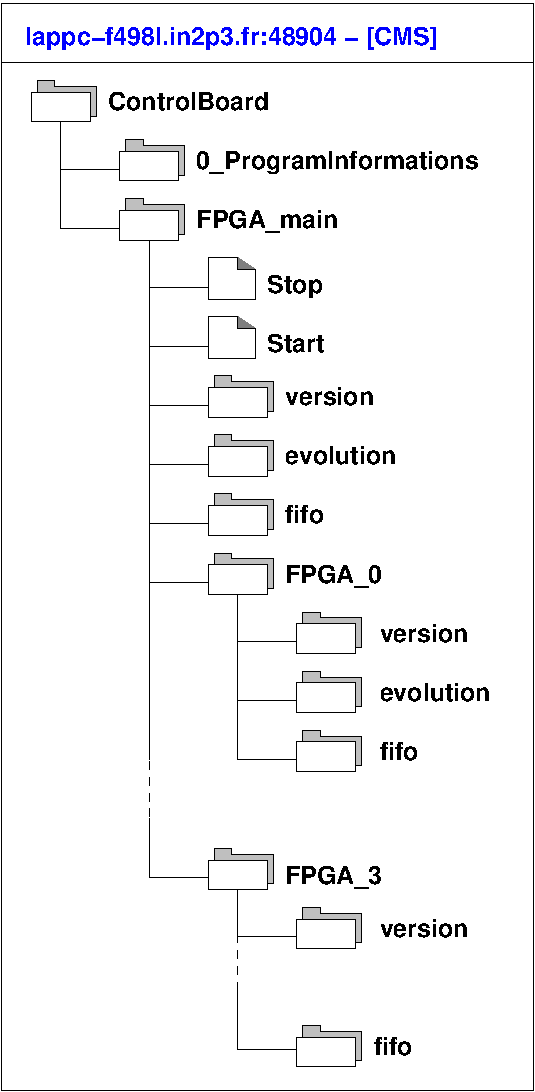
\includegraphics[width=5cm]{appendix/images/MOS_device_example_1.pdf}
\end{center}
\caption{Example of a  device managed through a MOS  server.  The root
  device is named \texttt{ControlBoard}.  First level daughter devices
  are  \texttt{0\_ProgramInformations} and  \texttt{FPGA\_main}.  Here
  the          MOS/OPCUA          server          is          labelled
  \texttt{CMS}.}\label{fig:an:mos_dev_1}
\end{figure}

% TODO


\subsection{Integration of a new device in the Vire environment}

The Vire  API also implements a  mechanism to describe a  hierarchy of
devices.  This  mechanism is independant  of the  one used in  the MOS
system but can  be easily made compatible with it.   This means that a
MOS  hierarchy  of devices  can  be  represented  in Vire.   The  Vire
hierarchy of  devices can  be considered as  some kind  of filesystem,
each device  being a folder with  its unique path, as  shown on figure
\ref{fig:an:mos_dev_2}.   The \emph{methods}  associated to  a devices
(or a datapoint) can be considered as plain executable files stored in
the  device's folder  : they  constitute the  set of  \emph{resources}
associated to the device.


\begin{figure}[h]
\begin{center}
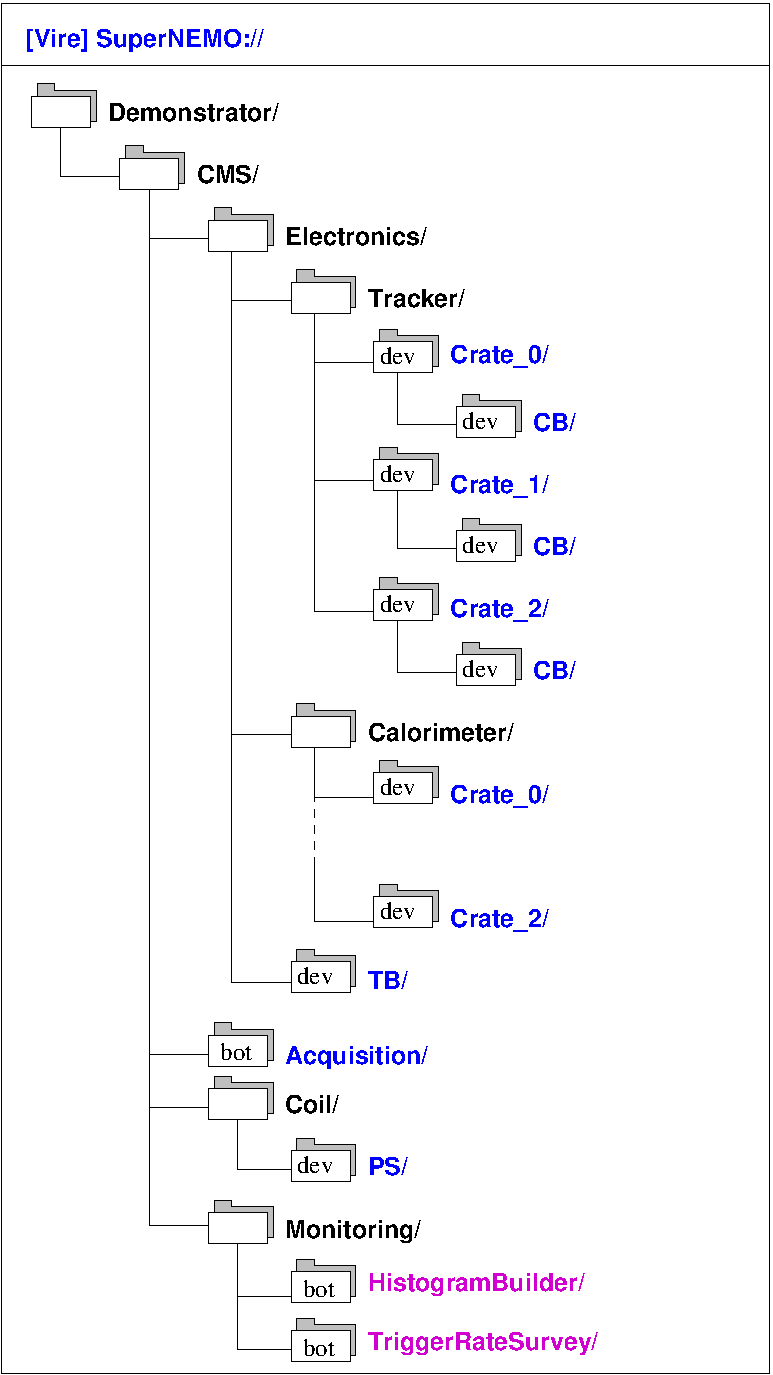
\includegraphics[width=5cm]{appendix/images/MOS_device_example_2.pdf}
\end{center}
\caption{Example of a hierarchy of  devices described by the Vire API.
  The root device is named  \texttt{SuperNEMO:}.  The top level (root)
  device  is  named  \texttt{Demonstrator}.  The  devices  colored  in
  \textcolor{blue}{blue}  are managed  through MOS/OPCUA.  The devices
  colored in \textcolor{magenta}{magenta} are directly embedded in the
  Vire server.  Devices with the \texttt{dev} tag are typical hardware
  device.  Devices  with the  \texttt{bot}  tag  are typical  software
  devices.   The  devices  colored in  \textbf{black}  are  structural
  pseudo-devices used to organize and  present a comprehensive view of
  the hierarchy. }\label{fig:an:mos_dev_2}
\end{figure}

The organisation of this hierarchy of devices is arbitrary and defined
by the designer of the  \emph{Control and Monitoring System}.  What is
important  to  understand  is  that  some  of  these  devices  can  be
associated  to  \emph{hardware  devices}  (a  power  supply  crate,  a
temperature probe\dots) and others  can be \emph{pseudo-devices}, i.e.
pure   software  object   (a   monitoring  robot,   a  file   transfer
daemon\dots).

In the context of the coupling of  the Vire server and the CMS server,
we are  in the event that  some devices are managed  by some MOS/OPCUA
servers and others are managed  in the Vire server itself.  Typically,
\emph{hardware devices}  are systematically managed through  the OPCUA
technology.  Vire has a mechanism to integrate such devices in its own
hierarchy.  This mechanism can  be considered like the \emph{mounting}
of   a   remote   filesystem   from  a   local   filesystem.    Figure
\ref{fig:an:mos_dev_0} illustrates  the case of many  hardware devices
-- managed by MOS -- that are integrated in the Vire system.  From the
Vire point of  view, the user does not see  the implementation details
for such  devices. He  does not  know the identity  of the  MOS server
hosting the device. He does not even know if the device is hosted by a
MOS server.  Devices are simply visible through the standard hierarchy
published by Vire with its  own device naming scheme, regardless their
true location.



\begin{figure}[h]
\begin{center}
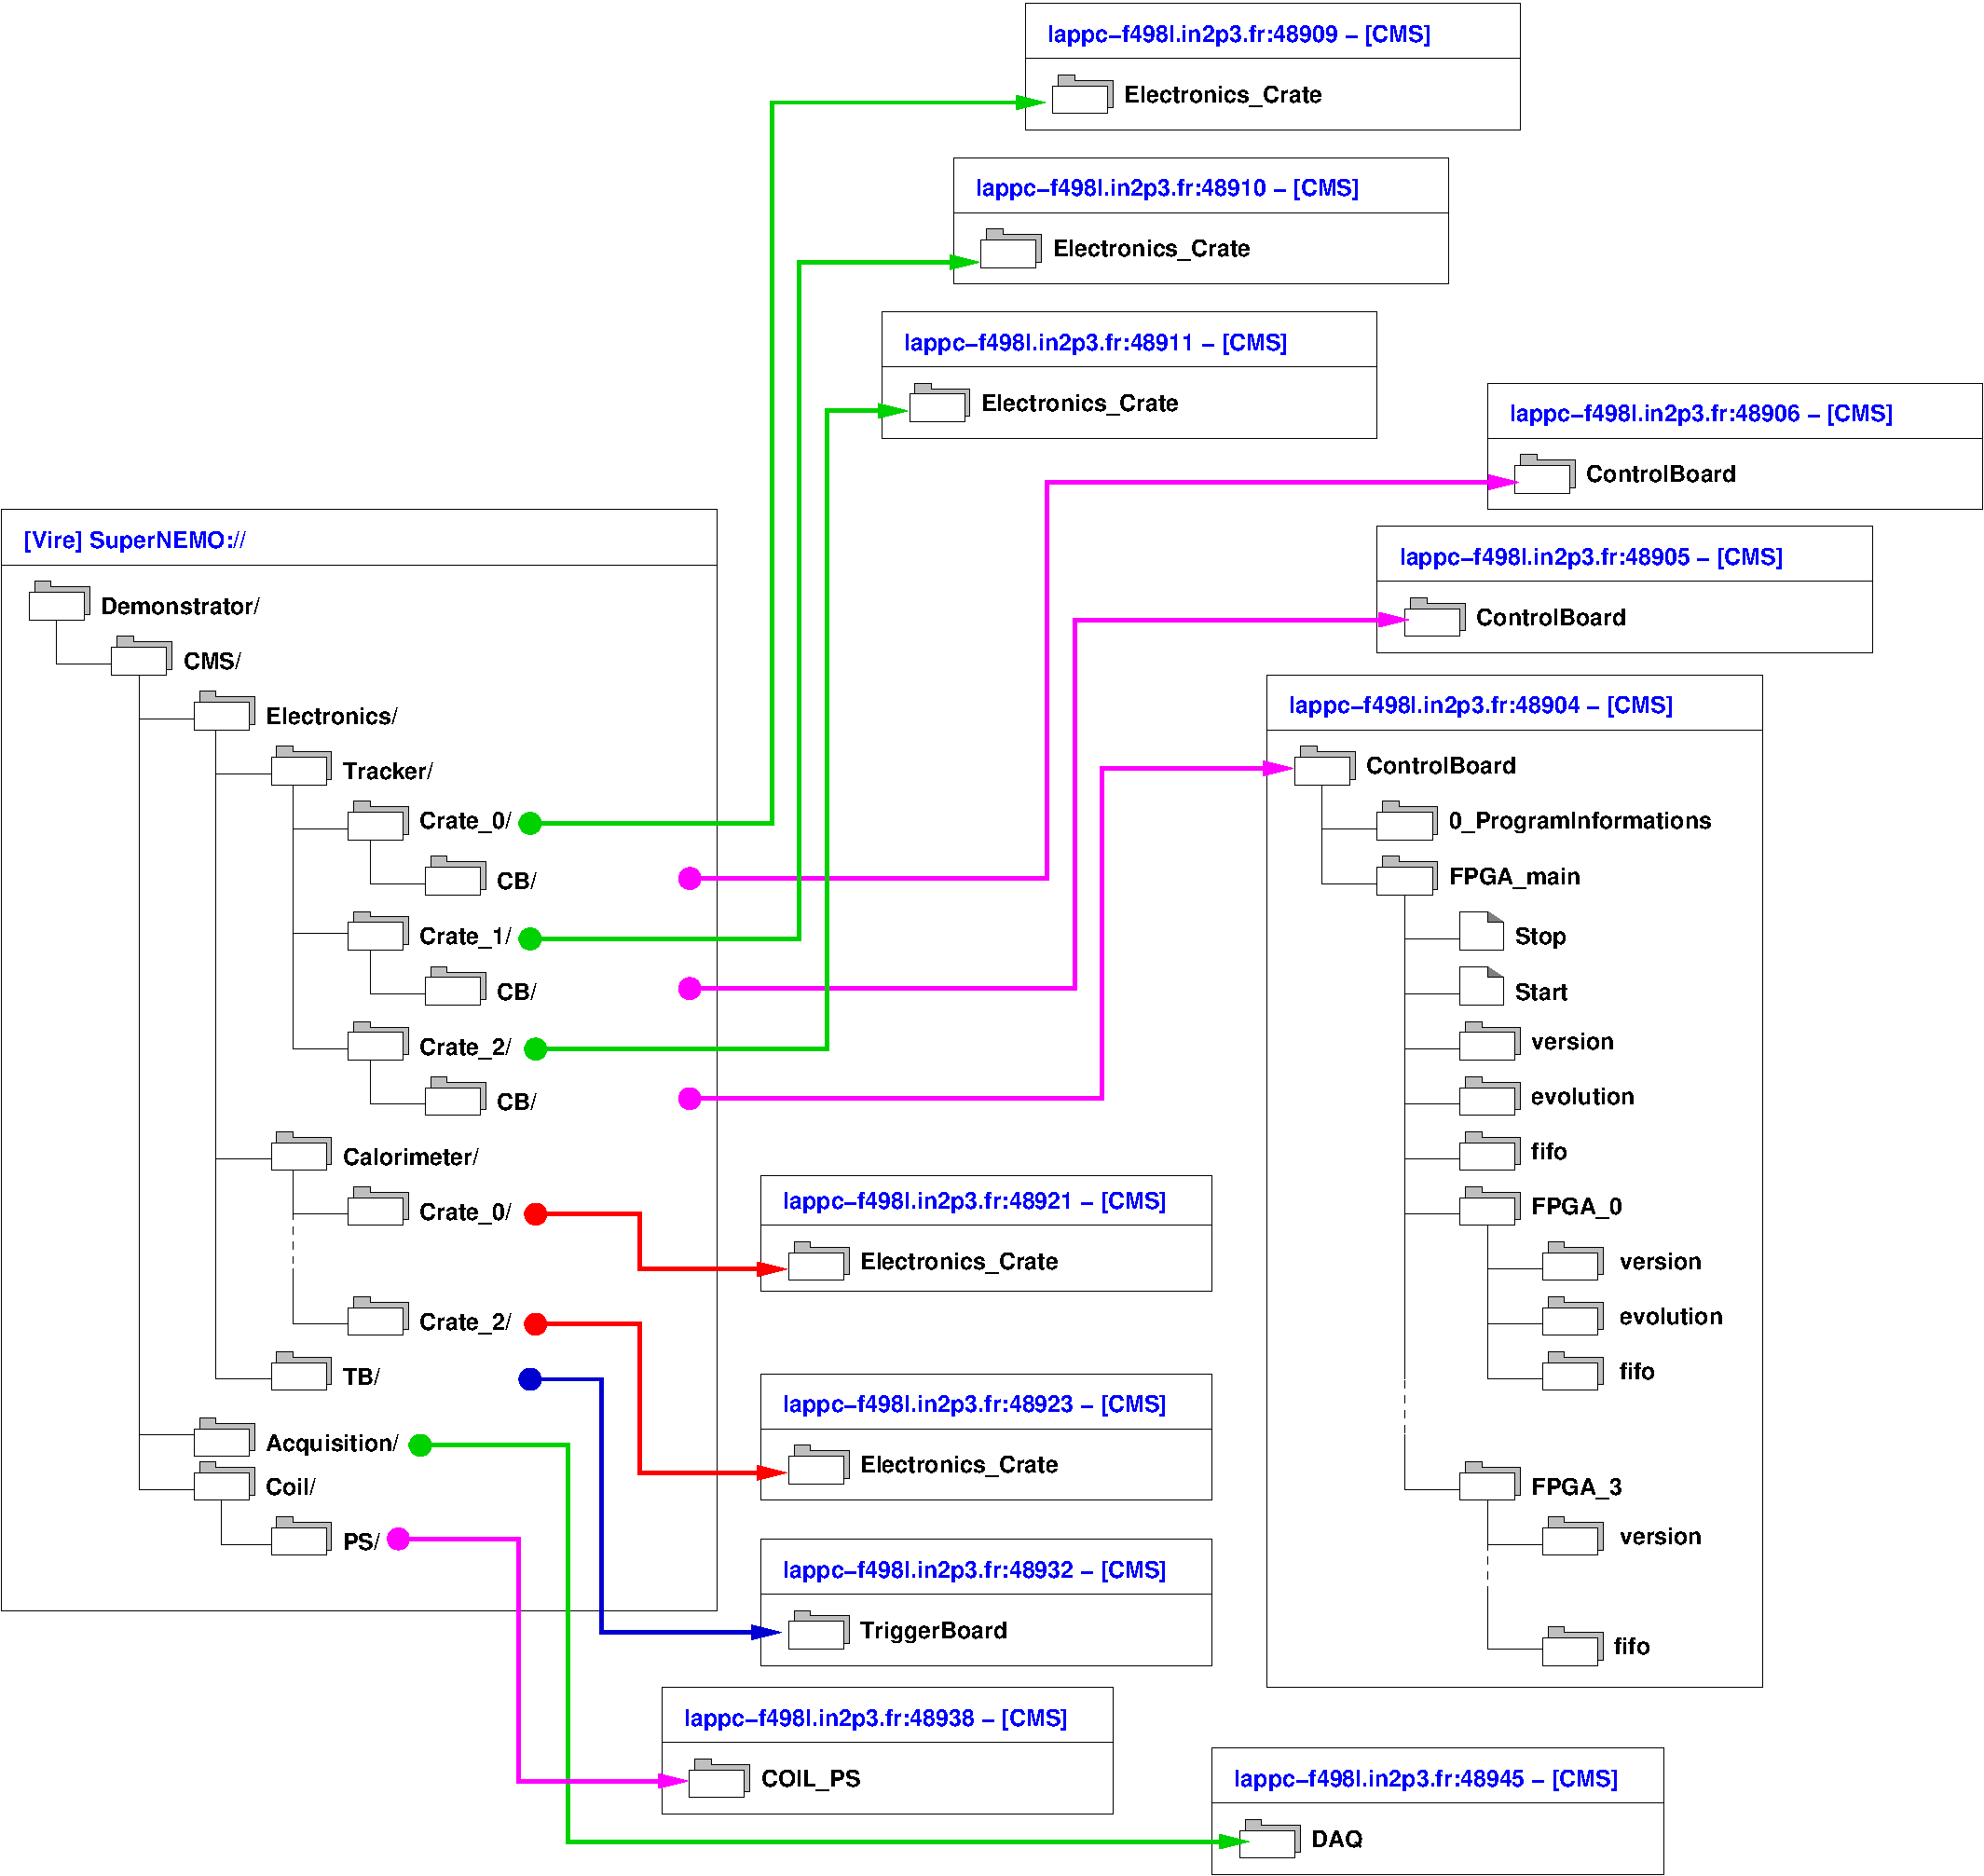
\includegraphics[width=\linewidth]{appendix/images/MOS_device_example_0.pdf}
\end{center}
\caption{The  mounting of  many  MOS device  hierarchies  in the  Vire
  device hierarchy.  Each OPCUA server  runs a simple  hardware device
  that is \emph{mounted} from a specific node with its own path.
%% of  devices described by the Vire API.
%%   The root device is named  \texttt{SuperNEMO:}.  The top level (root)
%%   device is  named \texttt{Demonstrator}. The devices  colored in blue
%%   are managed  through MOS/OPCUA. The  devices colored in  magenta are
%%   directly embedded in the Vire server.  Devices with the \texttt{dev}
%%   tag are typical  hardware device. Devices with  the \texttt{bot} tag
%%   are typical software devices.
}\label{fig:an:mos_dev_0}
\end{figure}




\subsection{Example}

Using  the examples  displayed  in  figure \ref{fig:an:mos_dev_0},  we
consider  in detail  the way  one specific  device managed  by MOS  is
mounted   in  the   Vire   hierarchy.  Figure   \ref{fig:an:mos_dev_3}
illustrates the mounting of a MOS device in Vire.

Here the Vire  server publishes the path of a  device representing the
control board  of the third  electronic crate  for the tracker  of the
SuperNEMO demonstrator module.  The full Vire path of this device is:

\textcolor{blue}{\texttt{SuperNEMO://Demonstrator/CMS/Electronics/Tracker/Crate\_2/CB}}

This is  the only Vire identifier  recognized by user to  address this
device.

On    the   figure,    one    can   see    that    the   MOS    server
\texttt{lappc−f498l.in2p3.fr} (port 48904) hosts a simple device which
is locally named \texttt{ControlBoard}.

When  mounting   this  device  in   the  Vire  hierarchy,   the  local
\texttt{[CMS]}  namespace and  \texttt{ControlBoard} device  names are
hidden and replaced by the Vire device path.  All daughter devices and
datapoints of  the \texttt{CMS/ControlBoard} device are  integrated as
daughters        of        the         Vire        device        named\\
\texttt{SuperNEMO://Demonstrator/CMS/Electronics/Tracker/Crate\_2/CB}.


For example, the \texttt{FPGA\_main} daughter device is now associated
to the following Vire path:

\textcolor{blue}{\texttt{SuperNEMO://Demonstrator/CMS/Electronics/Tracker/Crate\_2/CB/FPGA\_main/}}

and  its  \texttt{Stop} method  is  automatically  addressed with  the
following \emph{leaf} path:

\textcolor{blue}{\texttt{SuperNEMO://Demonstrator/CMS/Electronics/Tracker/Crate\_2/CB/FPGA\_main/Stop}}


\begin{figure}[h]
\begin{center}
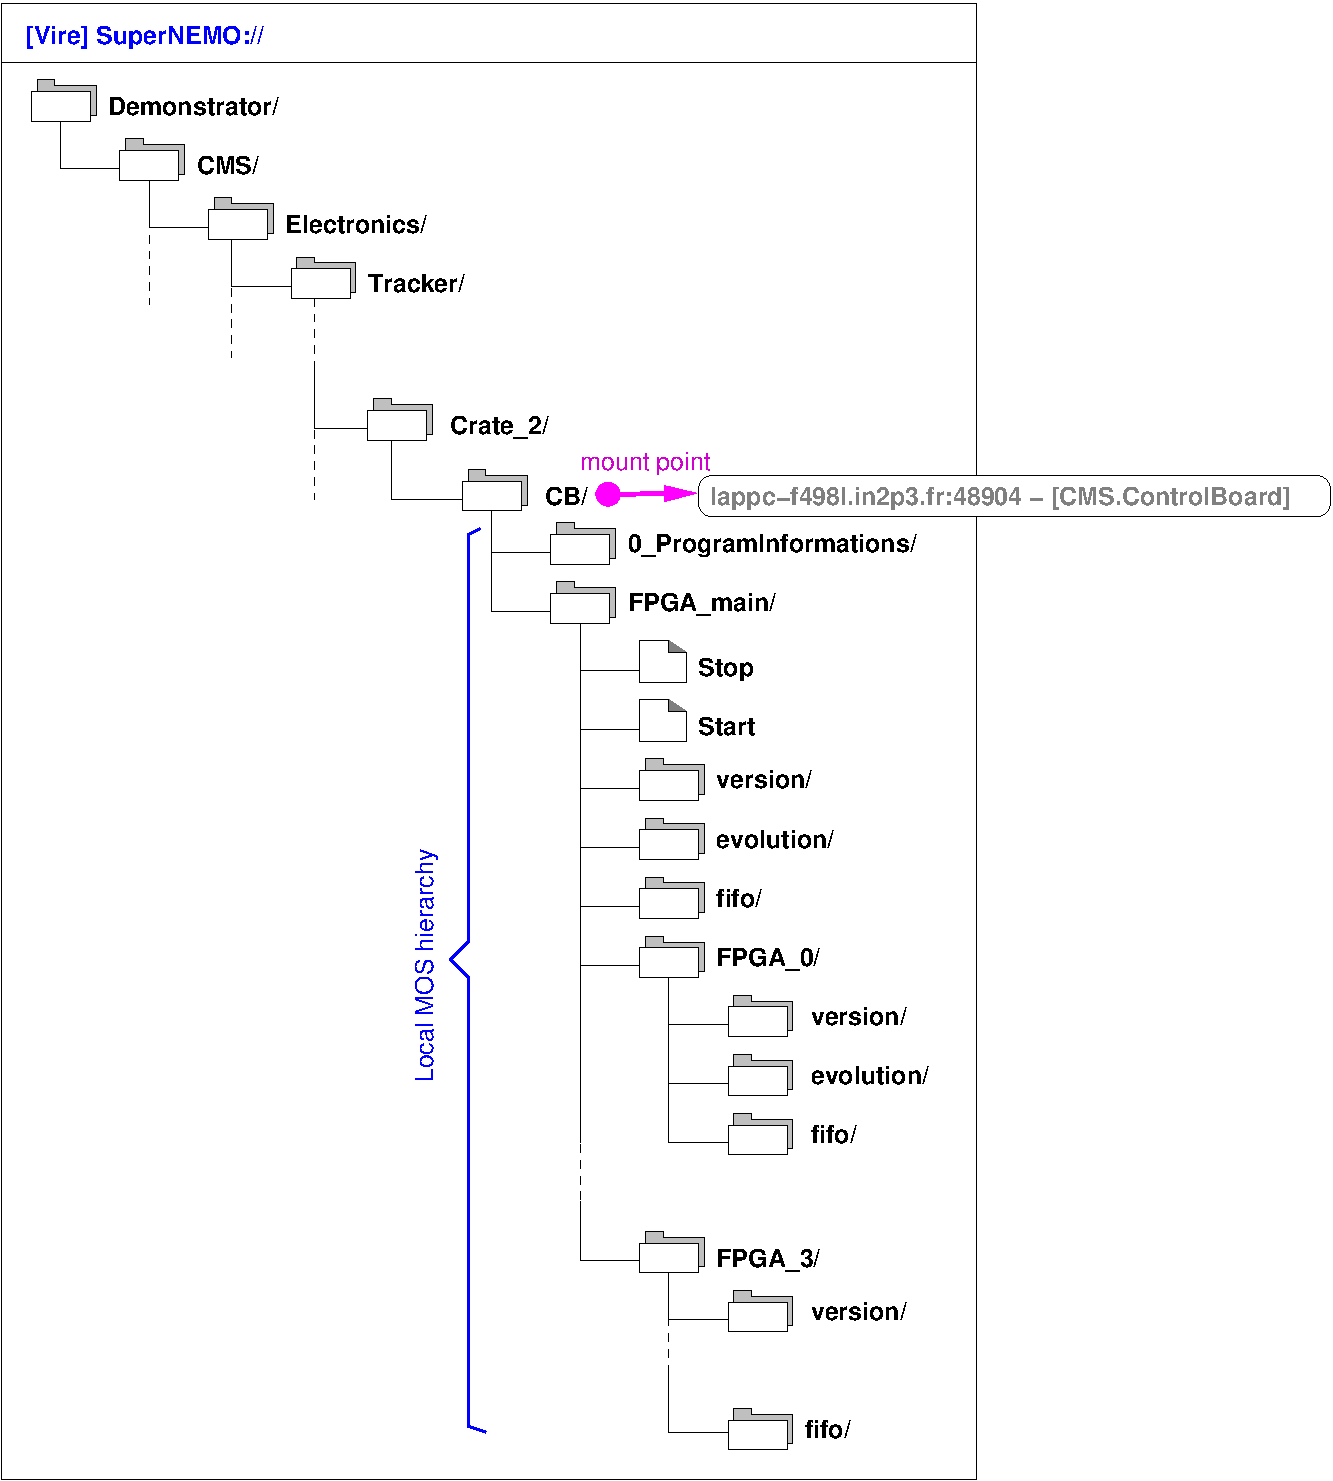
\includegraphics[width=0.8\linewidth]{appendix/images/MOS_device_example_3.pdf}
\end{center}
\caption{The  mounting of  one  MOS device and its local hierarchy  in the  Vire
  device hierarchy.}\label{fig:an:mos_dev_3}
\end{figure}



\subsection{Vire/MOS mapping}

As it can be  seen in the above example, the integration  of a new MOS
device in the Vire system is  achieved through soem kind of filesystem
mounting operation.   Particularly, it is  shown that the MOS  name of
the   mounted  root   device  is   replaced  by   an  arbitrary   Vire
path. However, all daughter  nodes (devices, datapoints) attached from
this root  node have their  relative MOS  names preserved in  the Vire
naming scheme.

Any  resource  (method)  associated  to any  of  such  daughter  nodes
inherits this relative naming scheme.

As Vire applications  describe resources through their  Vire paths, it
is thus needed to build an explicit map that associates resource paths
to MOS address  and name. The CMS  server will be able  to resolve the
MOS server/port and  embedded device associated to  the resource path.

The goal of the \texttt{devices\_launch.conf} file is not only to tell
the CMS server what MOS server should  be loaded and ran at start, but
also  to describe  the  \emph{mounting point/names}  used  by Vire  to
access the resources associated to MOS devices.  From the informations
stored in the  file, an explicit associative array must  be built when
the Vire server connect to the CMS server.  It will play the role of a
resource path resolver  when requests about resources will  be sent by
Vire applications.  This associative array  must be locked  during the
Vire/CMS connection.



%\subsubsection{Preparation of XML device models}

%% \noindent\underline{Pre-condition:}
%% The device is working and validated through the MOS/OPCUA server

%% \begin{enumerate}

%% \item Produce XML décrivant le modèle du device enrichi
%%   des metadata
%% Rédaction du fichier XML décrivant le modèle du device

%% \item Génération des fichiers model du type de device pour Vire

%% \item Génération des fichiers instances resolv.conf

%% \end{enumerate}


\vfill
\pagebreak
\clearpage

% end


\section{Vire messages}\label{app:vire_messages}

Within Vire  and between Vire  components and external  components, we
use  a communication  system  based on  Vire  messages.  This  section
describes the structure of such messages.

\subsection{General structure of a message}

Each message consists in two parts (figure \ref{fig-vire-message-message-cpp}):
\begin{itemize}

\item  the  \emph{header}  is   dedicated  to  generic  and  typicalle
  mandatory  informations  which  document   the  message  itself  and
  arbitrary high-level metadata.

\item  the \emph{body}  of the  message  contains the  real data: the payload.
  The structure of the message body depends on some convention. Vire uses
  its own convention to embed the payload data.

\end{itemize}

\begin{figure}[h]
\vskip 10pt
\small
\begin{Verbatim}[frame=single,xleftmargin=0.cm,label=\fbox{C++}]
struct vire::message::message {
  message_header header; // Header of the message
  message_body   body;   // Body of the message
};
\end{Verbatim}
\normalsize
\caption{The structure of a Vire message object (C++  class:
  \texttt{"vire::message::message"})}\label{fig-vire-message-message-cpp}
\end{figure}

\subsection{The message header}

The header contains (figure \ref{fig-vire-message-message_header-cpp}):
\begin{itemize}

  \item The mandatory \texttt{message\_id}  attribute is an identifier
    of the  message which  document the emitter  and a  unique message
    number.   Each emitter  is  responsible of  the  numbering of  the
    messages it  emits, typically using an  incremental technique. The
    message  number is  a positive  integer, starting  from 0  (figure
    \ref{fig-vire-message-message_identifier-cpp}).

  \item  The \texttt{timestamp}  attribute  encodes the  approximative
    time point when the message was  created. It contains the date and
    the time, using at least microsecond resolution.

    Typically,  with  JSON  encoding  system, it  is  expected  to  be
    formatted as a character string, using the following ISO format:

    \begin{center}
      \texttt{yyyymmddThhmmss.uuuuuu}
    \end{center}

    \noindent where:

    \vskip -10pt
    \begin{itemize}
    \item[\texttt{yyyymmdd} :] encodes year/month/day,
    \item[\texttt{hhmmssd} :] encodes hour/minute/second,
    \item[\texttt{uuuuuu} :] encodes microseconds.
    \end{itemize}

  \item   In   the   case    of   a   \emph{response}   message,   the
    \texttt{in\_reply\_to} attribute is set to identify the associated
    request message.

  \item  The \texttt{asynchronous}  boolean  attribute is  set if  the
    message processing  is explicitely requested  by the source  to be
    asynchronous (non-blocking).  In  RPC transactions, where requests
    are transmitted from one point to  the other, its default value is
    \emph{false}.   It  is possible  to  force  a RPC  transaction  in
    asynchronous mode.   This use  case is documented  elsewhere.  For
    event messaging, this flag is conventionally set to \emph{true}.

  \item  The  \texttt{body\_layout\_id}  attribute  is  the  mandatory
    identifier   of   the   layout   of  the   message   body   (class
    \texttt{"vire::utility::model\_identifier"}).  The  default layout
    for     message     body     inside    the     Vire     API     is
    \texttt{"vire::message::body\_format::typed\_payload"}, with version
    \texttt{"1.0"}                                             (figure
    \ref{fig-vire-utility-model_identifier-cpp}).

\end{itemize}


\begin{figure}[h]
\vskip 10pt
\small
\begin{Verbatim}[frame=single,xleftmargin=0.cm,label=\fbox{C++}]
struct vire::message::message_header {
  message_identifier message_id;     // Message identifier from the emitter.
  std::string        timestamp;      // Timestamp.
  message_identifier in_reply_to;    // Message identifier of the associated
                                     // request message (optional).
  bool               asynchronous,   // Asynchronous flag.
  vire::utility::model_identifier     body_layout_id; // Body layout identifier.
  std::map<std::string, std::string>  metadata;       // Key/value metadata dictionary.
};
\end{Verbatim}
\normalsize
\caption{The  structure  of  a   message  header  object  (C++  class:
  \texttt{"vire::message::message\_header"}).}\label{fig-vire-message-message_header-cpp}
\end{figure}

\begin{figure}[h]
\vskip 10pt
\small
\begin{Verbatim}[frame=single,xleftmargin=0.cm,label=\fbox{C++}]
struct vire::message::message_identifier {
  std::string emitter; // Name identifying the emitter of the message.
  int32_t     number;  // Number identifying the message in the emitter's
                       // message numbering scheme.
};
\end{Verbatim}
\normalsize
\caption{The      structure      of     a      message      identifier
  (C++  class:  \texttt{"vire::message::message\_identifier"}).}
\label{fig-vire-message-message_identifier-cpp}
\end{figure}

\begin{figure}[h]
\vskip 10pt
\small
\begin{Verbatim}[frame=single,xleftmargin=0.cm,label=\fbox{C++}]
struct vire::utility::model_identifier {
  std::string name;    // Name identifying the format of the message.
  std::string version; // String identifying the version of the format.
};
\end{Verbatim}
\normalsize
\caption{The structure of a model identifier (C++  class:  \texttt{"vire::utility::model\_identifier"}.}\label{fig-vire-utility-model_identifier-cpp}
\end{figure}




\begin{figure}[h]
\vskip 10pt
\small
\begin{Verbatim}[frame=single,xleftmargin=0.cm,label=\fbox{JSON}]
{
   "header" : {
      "message_id" : {
         "emitter" : "vire.server",
         "number" : 42
      },
      "timestamp" : "20160930T141408.413443",
      "in_reply_to" : {
         "initialized" : true,
         "value" : {
            "emitter" : "vire.client.0",
            "number" : 23
         }
      },
      "asynchronous" : false,
      "body_layout_id" : {
         "name" : "vire::message::body_format::typed_payload",
         "version" : {
            "initialized" : true,
            "value" : "1.0"
         }
      },
      "metadata" : [
         {
            "key" : "key1",
            "value" : "foo"
         },
         {
            "key" : "key2",
            "value" : "42"
         },
         {
            "key" : "key3",
            "value" : "3.1415899999999999"
         },
         {
            "key" : "key4",
            "value" : "true"
         }
      ]
   }
  "body" : {
      ...
   }
}
\end{Verbatim}
\normalsize
\caption{Example of  a   message  header  object in JSON format.}
\label{fig-vire-message-message_header-json}
\end{figure}

\vfill
\clearpage
\pagebreak

\subsection{The message body}

The    default    message   body    layout    in    Vire   is    named
\texttt{"vire::message::body\_format::typed\_payload"}        (version
\texttt{"1.0"}).   Each  message used  within  the  Vire framework  is
supposed to use this layout.  The general idea is that the body of the
message embeded the  \emph{payload object} that has  to be transmitted
between  two components  of  the system.   \emph{Payload objects}  are
classified in one of the three following categories:

\begin{enumerate}

\item \emph{Request}:  describes a request submitted  by one component
  to another component (generally during a synchronous RPC transaction).

\item  \emph{Response}: describes  the  response to  a former  request
  (generally during a synchronous RPC transaction).

\item \emph{Event}: describes an  arbitrary information record (alarm,
  exception, signal\dots) which is transmitted asynchronously.

\end{enumerate}

Vire implements the following class hierarchy:

\begin{center}
\begin{tikzpicture}
  \node (payload)  at (0,2)  [draw] {\texttt{vire::utility::base\_payload}};
  \node (request)  at (-4,0) [draw] {\texttt{vire::utility::base\_request}};
  \node (response) at (2,0)  [draw] {\texttt{vire::utility::base\_response}};
  \node (event)    at (8,0)  [draw] {\texttt{vire::utility::base\_event}};

  %\draw[style=help lines] (-3,-1) grid (10,4);
  \draw (node cs:name=response,anchor=north) |- (0,1);
  \draw (node cs:name=event,anchor=north)    |- (0,1);
  \draw[->] (node cs:name=request,anchor=north)
  |- (0,1) -| (node cs:name=payload,anchor=south);
\end{tikzpicture}
\end{center}

The requirements for the transmitted object are the following:

\begin{itemize}

\item The  type of the object  must be conventionally associated  to a
  unique     \emph{model      identifier}     object      (see     the
  \texttt{"vire::utility::model\_identifier"} class)  which contains a
  unique   name   (\textit{string    identifier})   and   possibly   a
  \textit{version identifier}.  Each software  component that may send
  or  receive the  object  should agree  on  this type  identification
  scheme.   This   enable  the  use  of   object  factories,  whatever
  programming  langage  is used  on  both  side of  the  communication
  system.

\item  For each  software component,  the object  type must  have some
  dedicated  encoding/decoding  functions  available  (again  whatever
  programming language is used). For example the Vire API supports the
  following encoding formats:

  \begin{itemize}

  \item JSON (MIME  encoding type: \texttt{"application/x-json"}), which
    is supportable by many languages,

  \item  Protobuf  (Google  Protocol   Buffers,  MIME  encoding  type:
    \texttt{"application/x-protobuf"}), which is also widely supported,

  \item   Boost/serialisation   (XML,    text   or   binary   archives
    \texttt{"application/x-boost-serialization-xml"},
    \texttt{"application/x-boost-serialization-text"},
    \texttt{"application/x-boost-serialization-binary"}),    which    in
    principle is supported by C++ only.

  \end{itemize}

  The Protobuf  encoding format will be  used to serialize/deserialize
  the  Vire  messages transported  between  the  Vire server  and  the
  CMS/LAPP server.

\end{itemize}

Vire uses a dedicated layout to represent the body of any message with
its embedded payload object. With this technique, the structure of the
body          contains         two          attributes         (figure
\ref{fig-app-vire-message-message_body-cpp}):

\begin{enumerate}

\item The \texttt{payload\_type\_id} specifies the type of the payload
  object   (figure   \ref{fig-app-vire-utility-model_identifier-cpp}).
  This unique name  is conventionaly fixed for a  given application. A
  version tag allows to support possible evolution of the object type.

\item The  \texttt{payload} is a  handle to  a payload object  of type
  request, response or event.

  %% \begin{itemize}
  %% \item Within  the producer  component of  the message,  the encoding
  %%   function associated to the object  type is responsible to generate
  %%   the JSON stream for the object and store it in the buffer.

  %% \item Within  the consumer  component of  the message,  the decoding
  %%   function associated to the object type is responsible to parse the
  %%   JSON stream stored in the buffer and restore the object in memory.

  %% \end{itemize}

  It is expected  that, on both sides of the  connection, the software
  components can  access dedicated  software plugins which  ensure the
  support  of  various   \emph{payload  object  types}  conventionnaly
  associated  with  their  \emph{payload type  identifiers}  and  also
  providing JSON and/or Protobuf encoding/decoding functionalities.

  %% The   system  allows  to  support
  %% modification  in the  structure of  the objects  thanks to  version
  %% tagging.

\end{enumerate}

\begin{figure}[h]
\vskip 10pt
\small
\begin{Verbatim}[frame=single,xleftmargin=0.cm,label=\fbox{C++}]
struct message_body {
  vire::utility::model_identifier     payload_type_id; // Object type identifier.
  const vire::utility::base_payload * payload;         // Handle to a payload object.
};
\end{Verbatim}
\normalsize
\caption{The structure of a message body object (C++).}
\label{fig-app-vire-message-message_body-cpp}
\end{figure}

\begin{figure}[h]
\vskip 10pt
\small
\begin{Verbatim}[frame=single,xleftmargin=0.cm,label=\fbox{JSON}]
{
  "header" : {
    ...
  },
  "body" : {
    "payload_type_id" : {
      "name" : "vire::message::testing::error_event",
      "version" : {
        "initialized" : false
      }
    },
    "payload" : {
      "timestamp" : "20160930T141743.759085"
      "err" : {
        "code" : 3,
        "message" : "A basic error"
      },
    }
  }
}
\end{Verbatim}
\normalsize
\caption{Example of  a   message  body  object in JSON format.}
\label{fig-vire-message-message_body-json}
\end{figure}

\vfill
\clearpage
\pagebreak

% end

%\input{appendix/app_json_fmt.tex}

\section{The \emph{Protocol Buffers} format}\label{app:protobuf_fmt}

\subsection{Introduction}

The  Google  Protocol Buffers  (\emph{protobuf})  library  is used  to
represent the objects that are exchanged between the Vire clients, the
Vire server and the CMS server.  The  version 3 of the format is used,
implying   at   least   version   3.0.0  (September   2016)   of   the
\emph{protobuf} library.

Each  data   structure  of  interest   can  be  described   through  a
\texttt{.proto}  file  from  which  stub files  can  be  automatically
generated  with the  \texttt{protoc} compiler.  For Vire  and its  CMS
interface, the C++ and Java programming languages will be used.


A  collection of  \texttt{.proto}  files are  provided  with the  Vire
library to represent all kind  of data structures transferable between
networked agents  (Vire server,  Vire clients, CMS/LAPP  server).  The
objects of  the highest level  are named \emph{payload  objects} (like
\emph{request},  \emph{response} and  \emph{event} objects).   They
are composed of attributes of more basic data structures.

\subsection{Example}

The following  class diagram  illustrates two data  structures defined
within the Vire library with an inheritance relationship between them.

\begin{center}
  \begin{tikzpicture}
    \node (base)     at (0,1.5)  [draw] {\texttt{vire::utility::base\_error}};
    \node (setup)    at (0,0)  [draw] {\texttt{vire::utility::invalid\_setup\_id\_error}};

    \draw[->]   (node cs:name=setup,anchor=north) |- (0,1);
    |- (0,1) -| (node cs:name=base,anchor=south);
  \end{tikzpicture}
\end{center}

The \texttt{vire::utility::base\_error}  is the  parent class  for all
\emph{error}  objects.   It  contains   two  attributes:   an  integer
\emph{error code}  and a  character string describing  the \emph{error
  message}.

The   \texttt{vire::utility::invalid\_setup\_id\_error}  class   is  a
specialized error class  which represents explicitely an  error due to
an identification  failure of  the experimental setup.   It implements
additional mutually exclusive attributes: the \emph{unrecognized name}
of the setup or the \emph{unrecognized version} of the setup.

This   example  illustrates   the  protobuf   representation  of   the
\texttt{vire::utility::base\_error}  in the  Vire  library, using  the
\texttt{"vire/utility/BaseError.proto"} file:

\small
\begin{Verbatim}[frame=single,xleftmargin=0.cm,label=\fbox{protobuf}]
  syntax = "proto3";
  package vire.utility; // Namespace

  message BaseError {

    // reserved 1; // Reserved for _base message

    // Attributes:
    int32  code           = 100; // The error code
    string message_format = 101; // The error description message

  }
\end{Verbatim}
\normalsize

\vfill
\clearpage
\pagebreak

\subsection{Vire protobuf conventions}

Vire uses the following conventions:

\begin{enumerate}

\item
  The member index  \texttt{1} is reserved to represent the  link of a
  class to its main base/parent class (if any).  It is not used if the
  data structure does not inherit any data structure.
  If a data structure naturally inherits another one, it is thus possible
  to  represent the  inheritance  relationship as  illustrated with  the
  \texttt{"vire/utility/InvalidSetupIdError.proto"}      file      which
  represents the \texttt{vire::utility::invalid\_setup\_id\_error} class
  in the Vire library:

  \small
  \begin{Verbatim}[frame=single,xleftmargin=0.cm,label=\fbox{protobuf}]
    syntax = "proto3";
    package vire.utility; // Namespace

    import "vire/utility/BaseError.proto"; // Dependency

    message InvalidSetupIdError {

      BaseError _base = 1; // The base class

      // Additional attributes:
      oneof detail { // Mutual exclusion
        string invalid_setup_name    = 100; // The failed setup name
        string invalid_setup_version = 101; // The failed setup version
      }

    }
  \end{Verbatim}
  \normalsize

\item The  \texttt{\_base} member  is conventionally  used to  represent the
  inheritance   relationship    from   a   data   structure    of   type
  \texttt{"vire.utility.BaseError"}.

\item Member indexes from \texttt{2}  to \texttt{99} are also reserved
  for possible future usage (multiple inheritance, metadata\dots).

\item
  The first member of the data structure must start at index \texttt{100}.

\end{enumerate}

\vfill
\clearpage
\pagebreak

% end


\section{Vire payload objects}\label{app:payload}

\subsection{Introduction}

As  mentioned in  appendix \ref{app:protobuf_fmt},  Vire messages  are
wrappers for \emph{payload objects}.  Each  type of payload object can
be represented  through the \emph{protobuf} mechanism.   The following
class hierarchy shows the base architecture used to define new payload
objects.

\begin{center}
\begin{tikzpicture}
  \node (payload)  at (0,2)   [draw] {\texttt{vire::utility::base\_payload}};
  \node (request)  at (-4,0)  [draw] {\texttt{vire::utility::base\_request}};
  \node (response) at (2,0)   [draw] {\texttt{vire::utility::base\_response}};
  \node (event)    at (8,0)   [draw] {\texttt{vire::utility::base\_event}};
  \node (my)       at (-4,-2) [draw] {\texttt{my\_request}};
  \node (your)     at (2,-2)  [draw] {\texttt{your\_response}};
  \node (its)    at (8,-2)    [draw] {\texttt{its\_alarm}};

  %\draw[style=help lines] (-6,-2) grid (10,2);
  \draw (node cs:name=response,anchor=north) |- (0,1);
  \draw (node cs:name=event,anchor=north)    |- (0,1);
  \draw[->] (node cs:name=request,anchor=north)
  |- (0,1) -| (node cs:name=payload,anchor=south);
  \draw[->] (node cs:name=my,anchor=north)
  |- (-4,-1) -| (node cs:name=request,anchor=south);
  \draw[->] (node cs:name=your,anchor=north)
  |- (2,-1) -| (node cs:name=response,anchor=south);
  \draw[->] (node cs:name=its,anchor=north)
  |- (8,-1) -| (node cs:name=event,anchor=south);
\end{tikzpicture}
\end{center}


\begin{center}
\vskip 10pt
\small
\begin{tabular}{|l|l|l|}
  \hline
  \textbf{Vire C++ class} & \textbf{protobuf message type} & \textbf{protobuf definition file} \\
  \hline
  \hline
  \multicolumn{3}{|c|}{\emph{general types}} \\
  \hline
  boost::posix\_time::ptime & google.protobuf.Timestamp & google/protobuf/timestamp.proto \\
  \hline
  \hline
  \multicolumn{3}{|c|}{\emph{identifier types}} \\
  \hline
  vire::utility::base\_identifier & vire.utility.Baseidentifier & vire/utility/Baseidentifier.proto \\
  \hline
  vire::utility::instance\_identifier & vire.utility.InstanceIdentifier & vire/utility/InstanceIdentifier.proto \\
  \hline
  vire::utility::model\_identifier & vire.utility.ModelIdentifier & vire/utility/ModelIdentifier.proto \\
  \hline
  \hline
  \multicolumn{3}{|c|}{\emph{error types}} \\
  \hline
  vire::utility::base\_error & vire.utility.BaseError & vire/utility/BaseError.proto \\
  \hline
  vire::utility::invalid\_context\_error & vire.utility.InvalidContextError & vire/utility/InvalidContextError.proto \\
  \hline
  vire::utility::invalid\_setup\_id\_error & vire.utility.InvalidSetupIdError & vire/utility/InvalidSetupIdError.proto \\
  \hline
  \hline
  \multicolumn{3}{|c|}{\emph{payload types}} \\
  \hline
  vire::utility::base\_payload & vire.utility.BasePayload & vire/utility/BasePayload.proto \\
  \hline
  vire::utility::base\_request & vire.utility.BaseRequest & vire/utility/BaseRequest.proto \\
  \hline
  vire::utility::base\_response & vire.utility.BaseResponse & vire/utility/BaseResponse.proto \\
  \hline
  vire::utility::base\_event & vire.utility.BaseEvent & vire/utility/BaseEvent.proto \\
  \hline
  vire::utility::base\_alarm & vire.utility.BaseAlarm & vire/utility/BaseAlarm.proto \\
  \hline
  \hline
  \multicolumn{3}{|c|}{\emph{messenging types}} \\
  \hline
  vire::message::message\_identifier & vire.message.MessageIdentifier & vire/message/MessageIdentifier.proto \\
  \hline
  vire::message::msg\_header & vire.message.MsgHeader & vire/message/MsgHeader.proto \\
  \hline
  vire::message::msg\_body & vire.message.MsgBody & vire/message/MsgBody.proto \\
  \hline
  vire::message::message & vire.message.Message & vire/message/Message.proto \\
  \hline
\end{tabular}
\normalsize
\end{center}


\begin{center}
\vskip 10pt
\small
\begin{tabular}{|l|l|l|}
  \hline
  \multicolumn{3}{|c|}{\emph{Resource management related types}} \\
  \hline
  vire::cms::resource\_status\_record & vire.cms.ResourceStatusRecord & vire/cms/ResourceStatusRecord.proto \\
  \hline
  vire::cms::resource\_fetch\_status\_request & vire.cms.ResourceFetchStatusRequest & vire/cms/ResourceFetchStatusRequest.proto \\
  \hline
  vire::cms::resource\_fetch\_status\_success\_response & vire.cms.ResourceFetchStatusSuccessResponse & vire/cms/ResourceFetchStatusSuccessResponse.proto \\
  \hline
  vire::cms::resource\_fetch\_status\_failure\_response & vire.cms.ResourceFetchStatusFailureResponse & vire/cms/ResourceFetchStatusFailureResponse.proto \\
  \hline
  vire::cms::resource\_exec\_request & vire.cms.ResourceExecRequest & vire/cms/ResourceExecRequest.proto \\
  \hline
  vire::cms::resource\_exec\_success\_response & vire.cms.ResourceExecSuccessResponse & vire/cms/ResourceExecSuccessResponse.proto \\
  \hline
  vire::cms::resource\_exec\_failure\_response & vire.cms.ResourceExecFailureResponse & vire/cms/ResourceExecFailureResponse.proto \\
  \hline
  vire::cms::resource\_exec\_non\_blocking\_request & vire.cms.ResourceExecNonBlockingRequest & vire/cms/ResourceExecNonBlockingRequest.proto \\
  \hline
  vire::cms::resource\_exec\_non\_blocking\_ack\_response & vire.cms.ResourceExecNonBlockingAckResponse & vire/cms/ResourceExecNonBlockingAckResponse.proto \\
  \hline
  vire::cms::resource\_exec\_non\_blocking\_noack\_response & vire.cms.ResourceExecNonBlockingNoackResponse & vire/cms/ResourceExecNonBlockingNoackResponse.proto \\
  \hline
  vire::cms::resource\_exec\_non\_blocking\_success\_event & vire.cms.ResourceExecNonBlockingSuccessEvent & vire/cms/ResourceExecNonBlockingSuccessEvent.proto \\
  \hline
  vire::cms::resource\_exec\_non\_blocking\_failure\_event & vire.cms.ResourceExecNonBlockingFailureEvent & vire/cms/ResourceExecNonBlockingFailureEvent.proto \\
  \hline
  vire::cms::resource\_exec\_error & vire.cms.ResourceExecError & vire/cms/ResourceExecError.proto \\
  \hline
  vire::cms::invalid\_status\_error & vire.cms.ResourceExecError & vire/cms/ResourceExecError.proto \\
  \hline
  %% vire::cms::invalid\_credentials\_error & vire.cms.InvalidCredentialsError & vire/cms/InvalidCredentialsError.proto \\
  %% \hline
  %% vire::cms::invalid\_user\_error & vire.cms.InvalidUserError & vire/cms/InvalidUserError.proto \\
  %% \hline
  vire::cms::invalid\_resource\_error & vire.cms.InvalidUserError & vire/cms/InvalidUserError.proto \\
  \hline
  vire::cms::no\_pubsub\_resource\_error & vire.cms.NoPubsubResourceError & vire/cms/NoPubsubResourceError.proto \\
  \hline
  \hline
  \multicolumn{3}{|c|}{\emph{Resource pub/sub management types}} \\
  \hline
  vire::cms::resource\_pubsub\_subscribe\_request & vire.cms.ResourcePubsubSubscribeRequest & vire/cms/ResourcePubsubSubscribeRequest.proto \\
  \hline
  vire::cms::resource\_pubsub\_subscribe\_success\_response & vire.cms.ResourcePubsubSubscribeRSuccessResponse & vire/cms/ResourcePubsubSubscribeRSuccessResponse.proto \\
  \hline
  vire::cms::resource\_pubsub\_subscribe\_failure\_response & vire.cms.ResourcePubsubSubscribeRFailureResponse & vire/cms/ResourcePubsubSubscribeRSuccessResponse.proto \\
  \hline
  \hline
  \multicolumn{3}{|c|}{\emph{Vire/CMS server interface types}} \\
  \hline
  vire::cmsinterface::connection\_request & vire.cmsinterface.ConnectionRequest & vire/cmsinterface/ConnectionRequest.proto \\
  \hline
  vire::cmsinterface::connection\_success\_response & vire.cmsinterface.ConnectionSuccessResponse & vire/cmsinterface/ConnectionSuccessResponse.proto \\
  \hline
  vire::cmsinterface::connection\_failure\_response & vire.cmsinterface.ConnectionFailureResponse & vire/cmsinterface/ConnectionFailureResponse.proto \\
  \emph{embedded:} unknown\_resources\_error & .UnknownResourcesError &  \\
  \hline
  vire::cmsinterface::disconnection\_request & vire.cmsinterface.DisconnectionRequest & vire/cmsinterface/DisconnectionRequest.proto \\
  \hline
  vire::cmsinterface::disconnection\_success\_response & vire.cmsinterface.DisconnectionSuccessResponse & vire/cmsinterface/DisconnectionSuccessResponse.proto \\
  \hline
  %% \hline
  %% vire::cmsinterface::disconnection\_failure\_response & vire.cmsinterface.DisconnectionFailureResponse & vire/cmsinterface/DisconnectionFailureResponse.proto \\
\end{tabular}
\normalsize
\end{center}

\subsection{Basic data structures}

Any  payload object  (request, response  or event)  generally contains
some information records which are  specific to the functionalities of
the  payload  object they  belong.   These  records are  of  arbitrary
types. Of course they should be  translatable in terms of the protobuf
library.
%Of course they can be (de)serialized using JSON.
Some of these types are very  general and defined within the Vire core
API itself because they are reused by various payload objects not only
through  the Vire-CMS/LAPP  interface  but also  between  Vire clients  and
servers, independently  of the  CMS/LAPP server.  However,  the use  of the
Protocol Buffers interface makes possible  to publish the interface of
such data to the outside world, including the CMS/LAPP server in priority.

%% Other one are specific to the Vire/CMS interface and thus managed only
%% in the \texttt{Vire\_CMSInterface} API.
These  types  are considered  as  \emph{basic}.  Among them  we  find:
generic error  types, generic  identifier types,  timestamps, resource
status records\dots We propose to describe them in this section.

Once a sufficient collection of  basic data record types is available,
it  is possible  to describe  high  level payload  object types  which
aggregate attributes of such types.

Other record  types are specific to  some payload objects and  will be
never  used outside  the scope  of these  payload objects.   Such data
structures will be  explicitely declared with the  payload object they
belong to, likely as embedded types/classes.


\subsubsection{Errors}

Some  \emph{response} or  \emph{event} payload  objects may  contain a
specific  error  record  object.   A  \emph{failure  response}  or  an
\emph{exception  event}  object will  generally  embed  such an  error
record object.

Each  \emph{error record}  is represented  by an  instance of  a given
error type.   Each of  the error  types defined  in Vire  inherits the
\texttt{vire::utility::base\_error}      base       class      (figure
\ref{fig-app-payload-base_error})   which   contains   the   following
attributes:

\begin{itemize}

\item the error code: A non zero  integer which is set to 1 by default
  (indicating  a  generic  failure  case).   The  error  code  can  be
  conventionally  set to  any positive  integer value  to represent  a
  specific error case, depending on the context.

\item the error  message: an optional human  readable character string
  which documents the error as usefully as possible.

\end{itemize}

\begin{figure}[h]
\vskip 10pt
\small
\begin{Verbatim}[frame=single,xleftmargin=0.cm,label=\fbox{C++}]
struct vire::utility::base_error
{
  // Attributes:
  int         code;           // Error code (>0).
  std::string message_format; // Error message (optional).
};
\end{Verbatim}
\normalsize
\caption{The structure of a \texttt{"vire::utility::base\_error"} object
  (C++).}
\label{fig-app-payload-base_error}
\end{figure}


%% An example of JSON formatted basic error object is given in figure
%% \ref{fig-app-payload-base_error-1}.
%%
%% \begin{figure}[h]
%% \vskip 10pt
%% \small
%% \begin{Verbatim}[frame=single,xleftmargin=0.cm,label=\fbox{\texttt{JSON}}]
%% {
%%   "code" : "42",
%%   "message_format" : "Invalid AMQP server port=[2341]"
%% }
%% \end{Verbatim}
%% \normalsize
%% \caption{JSON  formatted  basic  error  object  (class
%%   \texttt{vire::utility::base\_error}.}
%% \label{fig-app-payload-base_error-1}
%% \end{figure}

Several type of generic errors are defined in Vire:


\begin{center}
\begin{tikzpicture}
  \node (base)     at (0,2)  [draw] {\texttt{vire::utility::base\_error}};
  \node (context)  at (-4,0) [draw] {\texttt{vire::utility::invalid\_context\_error}};
  \node (setup)    at (0,-1)  [draw] {\texttt{vire::utility::invalid\_setup\_id\_error}};
  \node (resource) at (4,0)  [draw] {\texttt{vire::cms::invalid\_resource\_error}};
  \node (user)     at (8,-1)  [draw] {\texttt{vire::cms::invalid\_user\_error}};

  \draw     (node cs:name=setup,anchor=north)    |- (0,1);
  \draw     (node cs:name=resource,anchor=north) |- (0,1);
  \draw     (node cs:name=user,anchor=north)     |- (0,1);
  \draw[->] (node cs:name=context,anchor=north)
  |- (0,1) -| (node cs:name=base,anchor=south);
\end{tikzpicture}
\end{center}

\noindent
Here are a few error object types defined in Vire.  Some types belongs
to the \texttt{utility} namespace, other  ones are in the \texttt{cms}
namespace:

\begin{itemize}

\item \texttt{"vire::utility::invalid\_context\_error"} : occurs typically when
  the general context of the execution of a given resource is not adapted.\\
  It is mapped to the \texttt{"vire.utility.InvalidContextError"} protobuf record.

\item \texttt{"vire::utility::invalid\_setup\_id\_error"} : occurs in case
  of an invalid identification of the experimental setup managed
  by the Vire or CMS server.\\
  It is mapped to the \texttt{"vire.utility.InvalidSetupIdError"} protobuf record.

\item \texttt{"vire::cms::invalid\_resource\_error"} : occurs in case
  of an invalid identification of a resource.\\
  It is mapped to the  \texttt{"vire.cms.InvalidResourceError"} protobuf record.

\item \texttt{"vire::cms::invalid\_status\_error"}: occurs when an attempt
  to access a resource that has not the proper status.\\
  It is mapped to the  \texttt{"vire.cms.InvalidStatusError"} protobuf record.

\item \texttt{"vire::cms::invalid\_user\_error"} : occurs in case
  of an invalid identification of an user.\\
  It is mapped to the  \texttt{"vire.cms.InvalidUserError"} protobuf record.

\item \texttt{"vire::cms::invalid\_credentials\_error"} : occurs in case
  of user authentication error.\\
  It is mapped to the  \texttt{"vire.cms.InvalidCredentialsError"} protobuf record.

\item \texttt{"vire::cms::resource\_exec\_error"} : occurs in case
  of error at the execution of a given resource.\\
  It is mapped to the  \texttt{"vire.cms.ResourceExecError"} protobuf record.

\end{itemize}



\subsubsection{Object and type identifiers}

Vire  uses  some dedicated  classes  to  represent the  identifier  of
various objects  (or \emph{instances})  as well  as various  types (or
\emph{models})  of components.  Vire  implements  the following  class
hierarchy:

\begin{center}
\begin{tikzpicture}
  \node (base)  at (0,2)  [draw] {\texttt{vire::utility::base\_identifier}};
  \node (instance)  at (-4,0) [draw] {\texttt{vire::utility::instance\_identifier}};
  \node (model) at (4,0)  [draw] {\texttt{vire::utility::model\_identifier}};

  \draw (node cs:name=model,anchor=north) |- (0,1);
\draw[->] (node cs:name=instance,anchor=north)
  |- (0,1) -| (node cs:name=base,anchor=south);
\end{tikzpicture}
\end{center}

The          \texttt{vire::utility::base\_identifier}          (figure
\ref{fig-app-payload-base_identifier}) class is  a pure abstract class
that cannot be instantiated. However  it contains a mandatory name and
an  optional  version description  which  are  used by  all  inherited
classes:

\begin{itemize}

\item The   \texttt{vire::utility::instance\_identifier}    concrete   class
inherits  \texttt{vire::utility::base\_identifier}  and   is  used  to
identify \underline{unique instances of objects} known by the system.

\item The  \texttt{vire::utility::model\_identifier}   concrete  class  also
inherits  \texttt{vire::utility::base\_identifier}  and   is  used  to
identify \underline{types of objects} registered in the system.

\end{itemize}

The only difference between these two classes is the validation scheme
of  the name  attribute.

\begin{figure}[h]
\vskip 10pt
\small
\begin{Verbatim}[frame=single,xleftmargin=0.cm,label=\fbox{C++}]
struct base_identifier
{
  // Attributes:
  std::string name;    // The mandatory name uniquely identifying the object or
                       // the type of object.
  std::string version; // An optional character string representing the version
                       // of the object type.
};
\end{Verbatim}
\normalsize
\caption{The structure of the \texttt{vire::utility::base\_identifier}
  class (C++).}
\label{fig-app-payload-base_identifier}
\end{figure}

%%  Figure  \ref{fig-app-payload-identifier-json}
%% shows an example of instance indentifier.
%% \begin{figure}[h]
%% \vskip 10pt
%% \small
%% \begin{Verbatim}[frame=single,xleftmargin=0.cm,label=\fbox{\texttt{JSON}}]
%% {
%%   "name" : "vire::resource::invalid_resource_error",
%%   "version" : "1.0"
%% }
%% \end{Verbatim}
%% \normalsize
%% \caption{JSON  formatted class identifier  object (class
%%   \texttt{vire::utility::model\_identifier}).   Here one  identifies a
%%   specific error type.}
%% \label{fig-app-payload-identifier-json}
%% \end{figure}


\vfill
\pagebreak
\clearpage

\subsubsection{Resource related objects}

\begin{itemize}

\item
Class \texttt{vire::cms::invalid\_resource\_error} (figure \ref{fig-app-payload-invalid_resource_error}).

\begin{center}
\begin{tikzpicture}
  \node (base)  at (0,2)  [draw] {\texttt{vire::utility::base\_error}};
  \node (ire)  at (0,0) [draw] {\texttt{vire::cms::invalid\_resource\_error}};
  \draw[->] (node cs:name=ire,anchor=north)
  |- (0,1) -| (node cs:name=base,anchor=south);
\end{tikzpicture}
\end{center}

\begin{figure}[h]
\vskip 10pt
\small
\begin{Verbatim}[frame=single,xleftmargin=0.cm,label=\fbox{C++}]
struct vire::cms::invalid_resource_error : public vire::utility::base_error
{
  // Attributes:
  std::string invalid_resource_path; // Invalid resource path
  std::string invalid_resource_id;   // Invalid resource internal ID (Vire server only)
};
\end{Verbatim}
\normalsize
\caption{The structure  of a invalid resource error object (C++).}
\label{fig-app-payload-invalid_resource_error}
\end{figure}

\begin{figure}[h]
\vskip 10pt
\small
\begin{Verbatim}[frame=single,xleftmargin=0.cm,label=\fbox{JSON++}]
{
  "code" : "3",
  "message_format" : "Resource path 'Atlas://Calorimeter/HV/Crate1/stop' is invalid",
  "invalid_resource_path" : "Atlas://Calorimeter/HV/Crate1/stop"
}
\end{Verbatim}
\normalsize
\caption{JSON formatted invalid resource error object.}
\label{fig-app-payload-invalid_resource_error-json}
\end{figure}


\item
Class     \texttt{vire::cms::resource\_status\_record}    (figure
\ref{fig-app-payload-resource_status_record}).

\end{itemize}

\begin{figure}[h]
\vskip 10pt
\small
\begin{Verbatim}[frame=single,xleftmargin=0.cm,label=\fbox{C++}]
struct vire::cms::resource_status_record
{
  // Attributes:
  std::string path;      // Path of the resource
  std::string timestamp; // Timestamp of the last modification
  uint16_t    flags;     // Status bits (Missing/Disabled/Pending/Error)
};
\end{Verbatim}
\normalsize
\caption{The structure  of a resource status record object (C++).}
\label{fig-app-payload-resource_status_record}
\end{figure}


\begin{figure}[h]
\vskip 10pt
\small
\begin{Verbatim}[frame=single,xleftmargin=0.cm,label=\fbox{JSON}]
{
  "path" : "SuperNEMO://Demonstrator/CMS/Coil/Control/Current/__dp_read__",
  "timestamp" : "20160612T212432.324517",
  "flags" : 2
}
\end{Verbatim}
\normalsize
\caption{JSON formatted resource status record object.}
\label{fig-app-payload-resource_status_record-json}
\end{figure}

\vfill
\pagebreak
\clearpage

\subsection{Connection of the Vire server to the CMS server}


\begin{itemize}

\item   The   \texttt{vire::cmslapp::connection\_request}   class
  (version \texttt{1.0})  represents a connection request  sent by the
  Vire server to the  CMS server through the \textcolor{blue}{service}
  channel.

\begin{center}
\begin{tikzpicture}
  \node (base)  at (0,2)  [draw] {\texttt{vire::utility::base\_request}};
  \node (cr)  at (0,0) [draw] {\texttt{vire::cmslapp::connection\_request}};
  \draw[->] (node cs:name=cr,anchor=north)
  |- (0,1) -| (node cs:name=base,anchor=south);
\end{tikzpicture}
\end{center}

\noindent Class registration:
\begin{itemize}
\item name: \texttt{"vire::cmslapp::connection\_request"}
\item version: "1.0"
\end{itemize}

\begin{figure}[h]
\vskip 10pt
\small
\begin{Verbatim}[frame=single,xleftmargin=0.cm,label=\fbox{C++}]
struct vire::cmslapp::connection_request : public vire::utility::base_request
{
  // Attributes:
  vire::utility::instance_identifier  setup_id; // Identifier of the experimental setup
  std::vector<std::string> requested_resources; // The list of requested resources
                                                // addressed by path
};
\end{Verbatim}
\normalsize
\caption{The structure of the connection  request object to be emitted
  by the Vire server to the CMS server (C++).}
\label{fig-app-payload-connection_request}
\end{figure}

\begin{figure}[h]
\vskip 10pt
\small
\begin{Verbatim}[frame=single,xleftmargin=0.cm,label=\fbox{JSON}]
{
  "setup_id" : {
    "name" : "snemo",
    "version" : "1.0.2"
  },
  "requested_resources" : [
    "SuperNEMO://Demonstrator/CMS/Coil/PS/Control/Current/__dp_read__",
    "SuperNEMO://Demonstrator/CMS/Coil/PS/Control/Current/__dp_write__",
    ...
    "SuperNEMO://Demonstrator/CMS/Acquisition/start",
    "SuperNEMO://Demonstrator/CMS/Acquisition/stop"
  ]
}
\end{Verbatim}
\normalsize
\caption{A JSON formatted  connection request object sent  by the Vire
  server to the CMS server (C++).}
\label{fig-app-payload-connection_request-json}
\end{figure}


\item  The  \texttt{vire::cmslapp::connection\_success\_response}
  class represents  the response sent back  to the Vire server  by the
  CMS server through the  \textcolor{blue}{service} channel in case of
  success.

\begin{center}
\begin{tikzpicture}
  \node (base)  at (0,2)  [draw] {\texttt{vire::utility::base\_response}};
  \node (csr)  at (0,0) [draw] {\texttt{vire::cmslapp::connection\_success\_response}};
  \draw[->] (node cs:name=csr,anchor=north)
  |- (0,1) -| (node cs:name=base,anchor=south);
\end{tikzpicture}
\end{center}

\noindent Class registration:
\begin{itemize}
\item name: \texttt{"vire::cmslapp::connection\_success\_response"}
\item version: "1.0"
\end{itemize}

\begin{figure}[h]
\vskip 10pt
\small
\begin{Verbatim}[frame=single,xleftmargin=0.cm,label=\fbox{C++}]
struct connection_success_response
  : public vire::utility::base_response
{
  typedef vire::resource::resource_status_record resource_status_record; // Type alias

  // Attributes:
  std::vector<resource_status_record> resources_snapshot; // Requested resources snapshot
};
\end{Verbatim}
\normalsize
\caption{The structure  of the connection success  response emitted by
  the CMS server to the Vire server (C++).}
\label{fig-app-payload-connection_success_response}
\end{figure}



\begin{figure}[h]
\vskip 10pt
\small
\begin{Verbatim}[frame=single,xleftmargin=0.cm,label=\fbox{\texttt{JSON}}]
{
  "resources_snapshot"  : [
    {
      "path" : "SuperNEMO://Demonstrator/CMS/Coil/PS/Control/Current/__dp_read__",
      "timestamp" : "20160612T212432.324517",
      "flags" : "0000"
    },
    {
      "path" : "SuperNEMO://Demonstrator/CMS/Coil/PS/Control/Current/__dp_write__",
      "timestamp" : "20160612T212432.328732",
      "flags" : "0000"
    },
    ...
    {
      "path" : "SuperNEMO://Demonstrator/CMS/Acquisition/start",
      "timestamp" : "20160612T212432.371671",
      "flags" : "0000"
    },
    {
      "path" : "SuperNEMO://Demonstrator/CMS/Acquisition/stop",
      "timestamp" : "20160612T212432.373624",
      "flags" : "0100"
    }
  ]
}
\end{Verbatim}
\normalsize
\caption[JSON formatted  connection success response]  {JSON formatted
  connection        success        response       object        (class
  \texttt{vire::cmslapp::connection\_success\_response}.}
\label{fig-app-payload-connection_success_response-json}
\end{figure}


\item
The  \texttt{vire::cmslapp::connection\_failure\_response}  class
represents the response sent back to the Vire server by the CMS server
through the \textcolor{blue}{service} channel in case of failure.

\begin{center}
\begin{tikzpicture}
  \node (base)  at (0,2)  [draw] {\texttt{vire::utility::base\_response}};
  \node (cfr)  at (0,0) [draw] {\texttt{vire::cmslapp::connection\_failure\_response}};
  \draw[->] (node cs:name=cfr,anchor=north)
  |- (0,1) -| (node cs:name=base,anchor=south);
\end{tikzpicture}
\end{center}

\begin{figure}[h]
\vskip 10pt
\small
\begin{Verbatim}[frame=single,xleftmargin=0.cm,label=\fbox{C++}]
struct connection_failure_response
  : public vire::utility::base_response
{
  // Nested type alias:
  typedef vire::utility::model_identifier error_identifier;

  // Nested error type aliases:
  typedef vire::utility::invalid_context_error invalid_context_error;
  typedef vire::utility::invalid_setup_id_error invalid_setup_id_error;

  // Nested error type:
  struct unknown_resources_error : public vire::utility::base_error {
    std::vector<std::string> unknown_paths; // List of unknown resources' paths
  };

  // Attributes:
  error_identifier error_id; // Error type identifier
  XXX_error        error;    // Embedded error record of one of the nested error type above
};
\end{Verbatim}
\normalsize
\caption{The structure  of the  connection failure response emitted
  by the CMS server to the Vire server (C++).}
\label{fig-app-payload-connection_failure_response}
\end{figure}


\end{itemize}

% \texttt{vire::cmsserver::disconnection\_request} (version \texttt{1.0})

\vfill
\pagebreak
\clearpage


\subsection{Disconnection of the Vire server from the CMS server}

\begin{itemize}

\item  The  \texttt{vire::cmslapp::disconnection\_request}  class
  represents a  disconnection request sent  by the Vire server  to the
  CMS server through the \textcolor{blue}{service} channel.

\begin{center}
\begin{tikzpicture}
  \node (base)  at (0,2)  [draw] {\texttt{vire::utility::base\_request}};
  \node (cr)  at (0,0) [draw] {\texttt{vire::cmslapp::disconnection\_request}};
  \draw[->] (node cs:name=cr,anchor=north)
  |- (0,1) -| (node cs:name=base,anchor=south);
\end{tikzpicture}
\end{center}

\noindent Class registration:
\begin{itemize}
\item name: \texttt{"vire::cmslapp::disconnection\_request"}
\item version: "1.0"
\end{itemize}

\begin{figure}[h]
\vskip 10pt
\small
\begin{Verbatim}[frame=single,xleftmargin=0.cm,label=\fbox{C++}]
struct disconnection_request : public vire::utility::base_request {
};
\end{Verbatim}
\normalsize
\caption{The structure of the disconnection  request object to be emitted
  by the Vire server to the CMS server (C++).}
\label{fig-app-payload-disconnection_request}
\end{figure}

%% \begin{figure}[h]
%% \vskip 10pt
%% \small
%% \begin{Verbatim}[frame=single,xleftmargin=0.cm,label=\fbox{C++}]
%% {
%% }
%% \end{Verbatim}
%% \normalsize
%% \caption{A JSON formatted  connection request object sent  by the Vire
%%   server to the CMS server (C++).}
%% \label{fig-app-payload-connection_request-json}
%% \end{figure}


\item  The  \texttt{vire::cmslapp::disconnection\_success\_response}
  class represents  the response sent back  to the Vire server  by the
  CMS server through the  \textcolor{blue}{service} channel in case of
  success.

\begin{center}
\begin{tikzpicture}
  \node (base)  at (0,2)  [draw] {\texttt{vire::utility::base\_response}};
  \node (csr)  at (0,0) [draw] {\texttt{vire::cmslapp::disconnection\_success\_response}};
  \draw[->] (node cs:name=csr,anchor=north)
  |- (0,1) -| (node cs:name=base,anchor=south);
\end{tikzpicture}
\end{center}


\noindent Class registration:
\begin{itemize}
\item name: \texttt{"vire::cmslapp::disconnection\_success\_response"}
\item version: "1.0"
\end{itemize}

\begin{figure}[h]
\vskip 10pt
\small
\begin{Verbatim}[frame=single,xleftmargin=0.cm,label=\fbox{C++}]
struct disconnection_success_response
  : public vire::utility::base_response
{
};
\end{Verbatim}
\normalsize
\caption{The structure  of the disconnection success  response emitted by
  the CMS server to the Vire server (C++).}
\label{fig-app-payload-disconnection_success_response}
\end{figure}


\end{itemize}


\vfill
\pagebreak
\clearpage

\subsection{Resource related payload objects}

\subsubsection{Resource Pub/Sub service}

\begin{itemize}

\item  The \texttt{vire::resource::resource\_pubsub\_request} object is responsible of
  demanding the activation/deactivation of the Pub/Sub service associated to a given
  resource (fig. \ref{fig-app-payload-resource_pubsub_request}).

\begin{figure}[h]
\vskip 10pt
\small
\begin{Verbatim}[frame=single,xleftmargin=0.cm,label=\fbox{C++}]
struct resource_pubsub_request
  : public vire::utility::base_request
{
  // Attributes:
  std::string path;      // The resource path.
  bool        subscribe; // Pub/Sub service (un)subscribe flag.
};
\end{Verbatim}
\normalsize
\caption{The structure of the \texttt{vire::resource::resource\_pubsub\_request}
  class (C++).}
\label{fig-app-payload-resource_pubsub_request}
\end{figure}

\item The \texttt{vire::resource::resource\_pubsub\_success\_response}
  object encapsulate a  successfull response of the CMS  server to the
  Vire  server  concerning   the  subscription/unsubscription  of  the
  Pub/Sub     service    associated     to     a    given     resource
  (fig. \ref{fig-app-payload-resource_pubsub_success_response}).

\begin{figure}[h]
\vskip 10pt
\small
\begin{Verbatim}[frame=single,xleftmargin=0.cm,label=\fbox{C++}]
struct resource_pubsub_success_response
  : public vire::utility::base_response
{
  // Pub/Sub mechanism type alias:
  typedef vire::resource::amqp_mechanism_address amqp_mechanism_address;

  // Type alias:
  typedef vire::utility::model_identifier pubsub_mechanism_identifier;
  typedef boost::variant<
      amqp_mechanism_address
      > pubsub_address_type;

  // Attributes:
  std::string                 path;               // The resource path.
  bool                        subscribe;          // The effective (un)subscribe flag.
  pubsub_mechanism_identifier pubsub_mechanism_id; // The mechanism for accessing Pub/Sub service
  pubsub_address_type         pubsub_address;      // If activation is set, this describes the
                                                   // access to the Pub/Sub service.
};
\end{Verbatim}
\normalsize
\caption{The structure of the \texttt{vire::resource::resource\_pubsub\_success\_response}
  class (C++).}
\label{fig-app-payload-resource_pubsub_success_response}
\end{figure}

\small
\begin{Verbatim}[frame=single,xleftmargin=0.cm,label=\fbox{JSON++}]
{
  "path" : "SuperNEMO://Demonstrator/CMS/Coil/PS/Monitoring/__dp_read__",
  "subscribe" : "true",
  "pubsub_mechanism_id" : "vire::amqp",
  "pubsub_address" : {
     "server" : "snemo.amqp",
     "port" : 1234,
     "channel" : "snemo.amqp.cms.pubsub.WAqq7ERzs1",
     "binding" : "SuperNEMO://Demonstrator/CMS/Coil/PS/Monitoring/__dp_read__",
     "key" : "coil.monitoring.pubsub"
  }
}
\end{Verbatim}
\normalsize

\item    The   \texttt{vire::resource::amqp\_mechanism\_address}    object
  describes   the  access   to   Pub/Sub   service  through   RabbitMQ
  (fig. \ref{fig-app-payload-amqp_pubsub_access_type}).

\begin{figure}[h]
\vskip 10pt
\small
\begin{Verbatim}[frame=single,xleftmargin=0.cm,label=\fbox{C++}]
struct amqp_mechanism_address
{
  // Attributes:
  std::string server;  // The AMQP server
  int         port;    // The AMQP server port
  std::string channel; // The RabbitMQ Pub/Sub channel.
  std::string binding; // The binding dedicated to this Pub/Sub service.
  std::string key;     // The Pub/Sub specific key/topic.
};
\end{Verbatim}
\normalsize
\caption{The structure of the \texttt{vire::resource::amqp\_pubsub\_access\_type}
  class (C++).}
\label{fig-app-payload-amqp_pubsub_access_type}
\end{figure}


\item The \texttt{vire::resource::resource\_pubsub\_failure\_response}
  object describes a failure response  concerning a request on Pub/Sub
  service       associated       to       a       given       resource
  (fig. \ref{fig-app-payload-resource_pubsub_failure_response}).


\begin{figure}[h]
\vskip 10pt
\small
\begin{Verbatim}[frame=single,xleftmargin=0.cm,label=\fbox{C++}]
struct resource_pubsub_failure_response
  : public vire::utility::base_response
{
  // Nested type alias:
  typedef vire::utility::model_identifier error_type_identifier;

  // Nested error type aliases:
  typedef vire::utility::invalid_context_error  invalid_context_error;
  typedef vire::utility::invalid_resource_error invalid_resource_error;

  // Nested error type:
  struct no_pubsub_resource_error : public vire::utility::base_error {
    std::string path; // The path of the resource without Pub/Sub service support
  };

  typedef boost::variant<
     invalid_context_error,
     invalid_resource_error,
     no_pubsub_resource_error
     > error_type;

  // Attributes:
  error_type_identifier error_type_id; // Error type identifier.
  error_type            error;        // Embedded error record of one of
                                      // the nested error types above.
};
\end{Verbatim}
\normalsize
\caption{The structure of the \texttt{vire::resource::resource\_pubsub\_failure\_response}
  class (C++).}
\label{fig-app-payload-resource_pubsub_failure_response}
\end{figure}

\end{itemize}

\vfill
\pagebreak
\clearpage

\subsubsection{Fetching resource status}

\begin{center}
\begin{tikzpicture}
  \node (payload)  at (0,2) [draw] {\texttt{vire::utility::base\_request}};
  \node (request)  at (0,0) [draw] {\texttt{vire::resource::resource\_fetch\_status\_request}};
  \draw[->] (node cs:name=request,anchor=north)
  |- (0,1) -| (node cs:name=payload,anchor=south);
\end{tikzpicture}
\end{center}

\begin{itemize}

\item The \texttt{vire::resource::resource\_fetch\_status\_request} object
  demands to the CMS server an updated status record associated to a given resource
(fig. \ref{fig-app-payload-resource_fetch_status_request}).

\begin{figure}[h]
\vskip 10pt
\small
\begin{Verbatim}[frame=single,xleftmargin=0.cm,label=\fbox{C++}]
struct resource_fetch_status_request
  : public vire::utility::base_request
{
  // Attributes:
  std::string path; // Resource path.
};
\end{Verbatim}
\normalsize
\caption{The structure of a \texttt{vire::utility::resource\_fetch\_status\_request} object
  (C++).}
\label{fig-app-payload-resource_fetch_status_request}
\end{figure}

\item The \texttt{vire::resource::resource\_fetch\_status\_success\_response} object
  transmits the updated/current status record  associated to a given resource
(fig. \ref{fig-app-payload-resource_fetch_status_success_response}).

\begin{figure}[h]
\vskip 10pt
\small
\begin{Verbatim}[frame=single,xleftmargin=0.cm,label=\fbox{C++}]
struct resource_fetch_status_success_response
  : public vire::utility::base_response
{
  // Nested type alias:
  typedef vire::resource::resource_status_record resource_status_record;

  // Attributes:
  resource_status_record status; // The resource status record.
};
\end{Verbatim}
\normalsize
\caption{The structure of a \texttt{vire::utility::resource\_fetch\_status\_success\_response} object
  (C++).}
\label{fig-app-payload-resource_fetch_status_success_response}
\end{figure}



\item The \texttt{vire::resource::resource\_fetch\_status\_failure\_response} object
  describes a failure detected by the CMS server in response to a resource fetch status request.

\begin{figure}[h]
\vskip 10pt
\small
\begin{Verbatim}[frame=single,xleftmargin=0.cm,label=\fbox{C++}]
struct resource_fetch_status_failure_response
  : public vire::utility::base_response
{
  // Nested type alias:
  typedef vire::utility::model_identifier error_identifier;

  // Nested error type aliases:
  typedef vire::utility::invalid_context_error   invalid_context_error;
  typedef vire::resource::invalid_resource_error invalid_resource_error;

  // Attributes:
  error_identifier error_id; // Error type identifier
  XXX_error        error;    // Embedded error record of one of the nested error type above
};
\end{Verbatim}
\normalsize
\caption{The structure of a \texttt{vire::utility::resource\_fetch\_status\_failure\_response} object
  (C++).}
\label{fig-app-payload-resource_fetch_status_failure_response}
\end{figure}


\end{itemize}


\vfill
\pagebreak
\clearpage

\subsubsection{Synchronous/blocking resource execution}

\begin{center}
\begin{tikzpicture}
  \node (payload)  at (0,2)   [draw] {\texttt{vire::utility::base\_request}};
  \node (request)  at (0,0)  [draw] {\texttt{vire::resource::resource\_exec\_request}};
  \draw[->] (node cs:name=request,anchor=north)
  |- (0,1) -| (node cs:name=payload,anchor=south);
\end{tikzpicture}
\end{center}

\begin{itemize}

\item The \texttt{vire::resource::resource\_exec\_request} object represent a resource execution request
in blocking (synchronous) mode.


\begin{figure}[h]
\vskip 10pt
\small
\begin{Verbatim}[frame=single,xleftmargin=0.cm,label=\fbox{C++}]
struct resource_exec_request
  : public vire::utility::base_request
{
  // Type alias:
  typedef vire::resource::method_argument method_argument;

  // Attributes:
  std::string                  path;            // Resource path.
  std::vector<method_argument> input_arguments; // Embedded error record of one of
                                                // the nested error type above.
};
\end{Verbatim}
\normalsize
\caption{The structure of a \texttt{vire::utility::resource\_fetch\_status\_failure\_response} object
  (C++).}
\label{fig-app-payload-resource_fetch_status_failure_response}
\end{figure}

\item \texttt{vire::resource::resource\_exec\_success\_response}

\small
\begin{Verbatim}[frame=single,xleftmargin=0.cm,label=\fbox{C++}]
struct resource_exec_success_response
 : vire::utility::base_response
{
  // Type alias:
  typedef vire::resource::method_argument        method_argument;
  typedef vire::resource::resource_status_record resource_status_record;

  // Attributes:
  resource_status_record       status;               // Resource status
  std::string                  reception_timestamp;  // Request reception timestamp
  std::string                  completion_timestamp; // Execution completion timestamp
  std::vector<method_argument> output_arguments;     // Output arguments
};
\end{Verbatim}



\item \texttt{vire::resource::resource\_exec\_failure\_response}


\small
\begin{Verbatim}[frame=single,xleftmargin=0.cm,label=\fbox{C++}]
struct resource_exec_failure_response
 : vire::utility::base_response
{

  // Error type aliases:
  typedef vire::utility::invalid_context_error   invalid_context_error;
  typedef vire::resource::invalid_resource_error invalid_resource_error;
  typedef vire::resource::invalid_status_error   invalid_status_error;
  typedef vire::resource::resource_exec_error    resource_exec_error;

  // Type aliases:
  typedef vire::utility::model_identifier        error_type_identifier;
  typedef boost::variant<
      invalid_context_error,
      invalid_resource_error,
      invalid_status_error,
      resource_exec_error> error_type;

  // Attributes:
  error_type_identifier error_type_id; // Error type identifier
  error_type            error;        // Embedded error record

};
\end{Verbatim}

\end{itemize}


\vfill
\pagebreak
\clearpage

\subsubsection{Asynchronous/non-blocking resource execution}

\begin{center}
\begin{tikzpicture}
  \node (payload)  at (0,2)   [draw] {\texttt{vire::utility::base\_request}};
  \node (request_nb)  at (0,0)  [draw] {\texttt{vire::resource::resource\_exec\_non\_blocking\_request}};
  \draw[->] (node cs:name=request_nb,anchor=north)
  |- (0,1) -| (node cs:name=payload,anchor=south);
\end{tikzpicture}
\end{center}

\begin{itemize}

\item \texttt{vire::resource::resource\_exec\_non\_blocking\_request}
\small
\begin{Verbatim}[frame=single,xleftmargin=0.cm,label=\fbox{C++}]
struct resource_exec_non_blocking_request
  : public vire::utility::base_request
{
  // Type alias:
  typedef vire::resource::method_argument method_argument;

  // Attributes:
  std::string                  path;            // Resource path.
  std::vector<method_argument> input_arguments; // Embedded error record of one of
                                                // the nested error type above.

};
\end{Verbatim}

\item \texttt{vire::resource::resource\_exec\_non\_blocking\_ack\_response}


\small
\begin{Verbatim}[frame=single,xleftmargin=0.cm,label=\fbox{C++}]
struct resource_exec_non_blocking_ack_response
 : vire::utility::base_response
{
  // Type alias:
  typedef vire::resource::method_argument        method_argument;
  typedef vire::resource::resource_status_record resource_status_record;

  // Attributes:
  resource_status_record       status;
  std::string                  reception_timestamp;

};
\end{Verbatim}


\item \texttt{vire::resource::resource\_exec\_non\_blocking\_noack\_response}


\small
\begin{Verbatim}[frame=single,xleftmargin=0.cm,label=\fbox{C++}]
struct resource_exec_non_blocking_noack_response
  : vire::utility::base_response
{
  // Type alias:
  typedef vire::resource::resource_status_record resource_status_record;
  typedef vire::utility::model_identifier error_type_identifier;

  // Error type aliases:
  typedef vire::utility::invalid_context_error   invalid_context_error;
  typedef vire::resource::invalid_resource_error invalid_resource_error;
  typedef vire::resource::invalid_status_error   invalid_status_error;
  typedef vire::resource::resource_exec_error    resource_exec_error;

  // Nested error type:
  struct no_non_blocking_exec_resource_error : public vire::utility::base_error {
    std::string path; // The path of the resource without non-blocking execution support
  };

  typedef boost::variant<
     invalid_context_error,
     invalid_resource_error,
     invalid_status_error,
     no_non_blocking_exec_resource_error,
     resource_exec_error
     > error_type;

  // Attributes:
  resource_status_record status;        // Resource status.
  error_type_identifier  error_type_id; // Error type identifier.
  error_type             error;         // Embedded error record of one of
                                        // the nested error types above.

};
\end{Verbatim}
\normalsize


\item \texttt{vire::resource::resource\_exec\_non\_blocking\_success\_event}


\small
\begin{Verbatim}[frame=single,xleftmargin=0.cm,label=\fbox{C++}]
struct resource_exec_non_blocking_success\_event
  : vire::utility::base_event
{
  // Type alias:
  typedef vire::resource::method_argument        method_argument;
  typedef vire::resource::resource_status_record resource_status_record;

  // Attributes:
  resource_status_record       status;               // Resource status
  std::string                  reception_timestamp;  // Request reception timestamp
  std::string                  completion_timestamp; // Execution completion timestamp
  std::vector<method_argument> output_arguments;     // Output arguments

};
\end{Verbatim}
\normalsize

\item \texttt{vire::resource::resource\_exec\_non\_blocking\_failure\_event}


\small
\begin{Verbatim}[frame=single,xleftmargin=0.cm,label=\fbox{C++}]
struct resource_exec_non_blocking_failure\_event
  : vire::utility::base_event
{

  // Error type aliases:
  typedef vire::utility::invalid_context_error   invalid_context_error;
  typedef vire::cms::invalid_resource_error invalid_resource_error;
  typedef vire::cms::invalid_status_error   invalid_status_error;
  typedef vire::cms::resource_exec_error    resource_exec_error;

  // Type aliases:
  typedef vire::utility::model_identifier        error_type_identifier;
  typedef boost::variant<
      vire::utility::invalid_context_error,
      vire::cms::invalid_resource_error,
      vire::cms::invalid_status_error,
      vire::cms::resource_exec_error> error_type;

  // Attributes:
  error_type_identifier error_type_id; // Error type identifier
  error_type            error;        // Embedded error record

};
\end{Verbatim}
\normalsize


\end{itemize}


\vfill
\pagebreak
\clearpage

% end


\section{The RabbitMQ based RPC system}\label{app:rabbitmq_rpc}

\subsection{Introduction}


\end{document}
%%

\section{Interaction of the CMS/LAPP server with Vire clients}

TODO
\vfill
\pagebreak
\clearpage

%%%%%%%%%
\appendix


\section{Filesystem and configuration files management}\label{app:filesystem_conf}

Let's consider  a simple  situation where  one runs  the Vire  and CMS
software  tools (servers)  on a  single Linux  machine (the  CMS host)
under            the            \texttt{"nemoprod"}            generic
account\footnote{\texttt{"nemoprod"}  is  the   login  of  th  generic
  account used at the CCIN2P3  cluster to perform automated management
  operations on experimental and  Monte-Carlo data file: data transfer
  from LSM or LSC labs to CCIN2P3, calibration and reconstruction data
  processing, storage on HPPS.}.

\begin{itemize}
\item Hostname login : \verb|192.168.1.10| (private IP) %\texttt{snemocms.lsm.in2p3.fr} (public address)
\item User login : \texttt{nemoprod}
\item Main group : \texttt{supernemo}
\item Home directory : \verb|/home/nemoprod| (a.k.a. \verb|~nemoprod|)
\end{itemize}

\noindent  We  assume that  the  SuperNEMO  online software  has  been
installed   and  setup   in  the   home  directory,   for  example in
\verb|/home/nemoprod/Private/Software/| :
\vskip 20pt
\small
\begin{Verbatim}[frame=single,xleftmargin=0.cm,label=\fbox{Filesystem}]
/home/nemoprod/Private/Software
|-- Cadfael/ # base directory of the Cadfael software framework
|-- Bayeux/  # base directory of the Bayeux software framework
|-- Vire/    # base directory of the Vire software framework
|-- OPCUA/   # base directory of the OPCUA+MOS software framework
`-- Falaise/ # base directory of the Falaise software framework
\end{Verbatim}
\normalsize

\noindent  We consider  here  that the  Falaise  library package  will
contain  the mandatory  configuration files  that describe  the online
software, both for the Vire and CMS/MOS parts:
\vskip 20pt
\small
\begin{Verbatim}[frame=single,xleftmargin=0.cm,label=\fbox{Filesystem}]
/home/nemoprod/Private/Software
:
`-- Falaise/
    :
    `-- Install/
        `-- Falaise-3.0.0/
            |-- bin/
            |   :
            |   |-- flquery
            |   |-- flreconstruct
            |   `-- flsimulate
            |-- include/
            :   :
            |-- lib/
            |   `-- x86_64-linux-gnu/
            |       :
            |       |-- libFalaise.so
            |       :
            `-- share/
                `-- Falaise-3.0.0/
                    `-- resources/
                        `-- config/
                            `-- online/
                                :
                                :
\end{Verbatim}
\normalsize

\noindent Where:
\begin{itemize}
\item                                                              the
  \verb|/home/nemoprod/Private/Software/Falaise/Install/Falaise-3.0.0|
  is  the  installation  prefix  of  the  Falaise  library  (binaries,
  includes) and associated resource files.
\item      the     \verb|share/Falaise-3.0.0/resources/config/online/|
  subdirectory  is the  tree  of configuration  files  that should  be
  accessible  by  any online  software  component  (Vire server,  Vire
  clients, CMS and MOS servers).
\end{itemize}


\noindent  Let's consider  the \verb|.../config/online/|  directory as
the base directory for all online configuration files for the Vire and
CMS  servers.   All  configuration  files  should  thus  be  addressed
relatively to this place.

\noindent  We  propose to  use  one  of  the following  techniques  to
represent this base directory:

\begin{itemize}
\item         a         dedicated         environment         variable
  \verb|SNEMO_ONLINE_CONFIG_BASE_DIR| recognized by  both Vire and CMS
  servers. It could be setup within the environment with:
\vskip 20pt
\small
\begin{Verbatim}[frame=single,xleftmargin=0.cm,label=\fbox{shell}]
export FALAISE_INSTALL_DIR=\
  ${HOME}/Private/Software/Falaise/Install/Falaise-3.0.0
export SNEMO_ONLINE_CONFIG_BASE_DIR=\
  ${FALAISE_INSTALL_DIR}/share/Falaise-3.0.0/resources/config/online
\end{Verbatim}
\normalsize

\item a  path registration label as  implemented in the kernel  of the
  Bayeux library:\\
  \noindent The \verb|@snonlinecfg:| label \\
  is associated to\\
  \noindent \hskip 50pt\verb|${FALAISE_INSTALL_DIR}/share/Falaise-3.0.0/resources/config/online|

\end{itemize}

\noindent Thus a specific  configuration file \verb|dummy.conf| could be
addressed with one of the following syntaxes:

\begin{itemize}

\item[(a)]
  \verb|${SNEMO_ONLINE_CONFIG_BASE_DIR}/snemo/1.0.2/dummy.conf|       :
  supported  by  Vire  and  CMS  using  word  expansion  utility  like
  \texttt{wordexp} (for C/C++ languages),

\item[(b)]  \verb|@snonlinecfg:snemo/1.0.2/dummy.conf|  : supported  by
  Vire  only  for  now,  thanks to  the  path  registration  mechanism
  implemented in the Bayeux API,

\item[(c)] \verb|snemo/1.0.2/dummy.conf| : can be supported by Vire and
  CMS  but  is  ambiguous  because  such a relative  path  can  be  also
  interpreted as a path relatively  to the current directory (\verb|./|)
  and not to the online configuration directory.

\end{itemize}

We suggests  the use  of an  explicit environment  variable as  in (a)
because it  is simple to  implement in various languages  and software
frameworks and should not imply any ambiguous file path resolution.

\vfill
\pagebreak
\clearpage

% end


\section{Integration of a new device}\label{app:new_device}

Both Vire  and MOS systems are  designed to be expandable  in terms of
device integration.  This section  decribes the  integration of  a new
device in the \emph{Control and Monitoring System}.

\subsection{Integration of a new device in the MOS environment}

Any new device is described through  a dedicated XML model file.  This
XML  file  is  created  from  a  template  file  elaborated  from  the
\emph{interface control document} (ICD) and associated to the model of
the  device. The  format  of the  XML  file is  described  in the  MOS
(Multipurpose OPCUA Server) User Guide. % ref

Typically, a device is embedded in a OPCUA server and implemented as a
OPCUA  \emph{simple  device}.   The  OPCUA server  itself  is  located
through an unique dedicated IP address and port.

The simple device  instance, hosted in the OPCUA  server, may contains
other sub-devices and/or \emph{datapoints}.   It is thus considered as
the root  of a hierarchy  of daughter  objects at deeper  levels.  The
daughter objects (devices or datapoints) are named relatively to their
top level  parent device. Figure  \ref{fig:an:mos_dev_1} shows an
example of a device embedded in a MOS server.

\begin{figure}[h]
\begin{center}
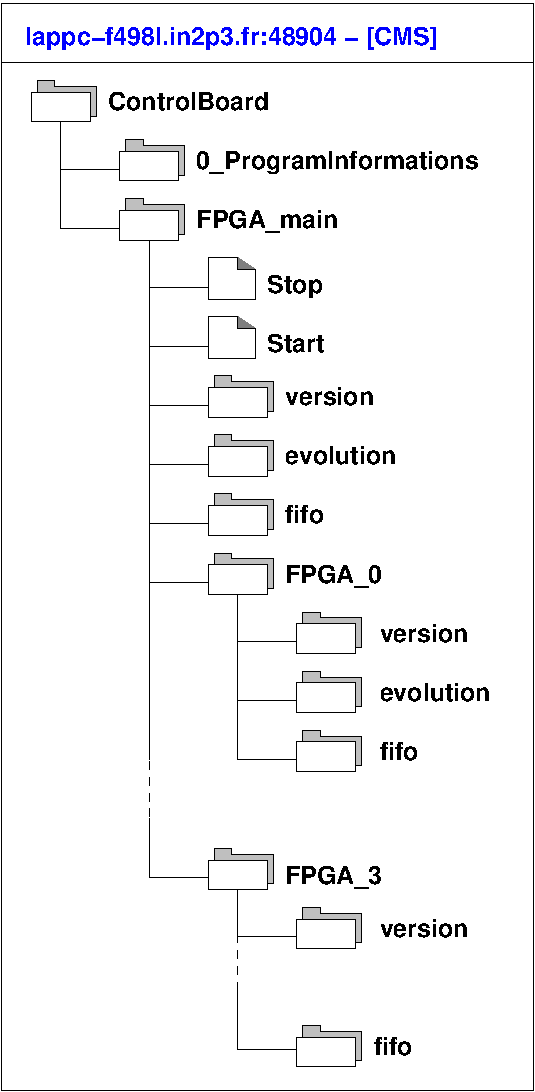
\includegraphics[width=5cm]{appendix/images/MOS_device_example_1.pdf}
\end{center}
\caption{Example of a  device managed through a MOS  server.  The root
  device is named \texttt{ControlBoard}.  First level daughter devices
  are  \texttt{0\_ProgramInformations} and  \texttt{FPGA\_main}.  Here
  the          MOS/OPCUA          server          is          labelled
  \texttt{CMS}.}\label{fig:an:mos_dev_1}
\end{figure}

% TODO


\subsection{Integration of a new device in the Vire environment}

The Vire  API also implements a  mechanism to describe a  hierarchy of
devices.  This  mechanism is independant  of the  one used in  the MOS
system but can  be easily made compatible with it.   This means that a
MOS  hierarchy  of devices  can  be  represented  in Vire.   The  Vire
hierarchy of  devices can  be considered as  some kind  of filesystem,
each device  being a folder with  its unique path, as  shown on figure
\ref{fig:an:mos_dev_2}.   The \emph{methods}  associated to  a devices
(or a datapoint) can be considered as plain executable files stored in
the  device's folder  : they  constitute the  set of  \emph{resources}
associated to the device.


\begin{figure}[h]
\begin{center}
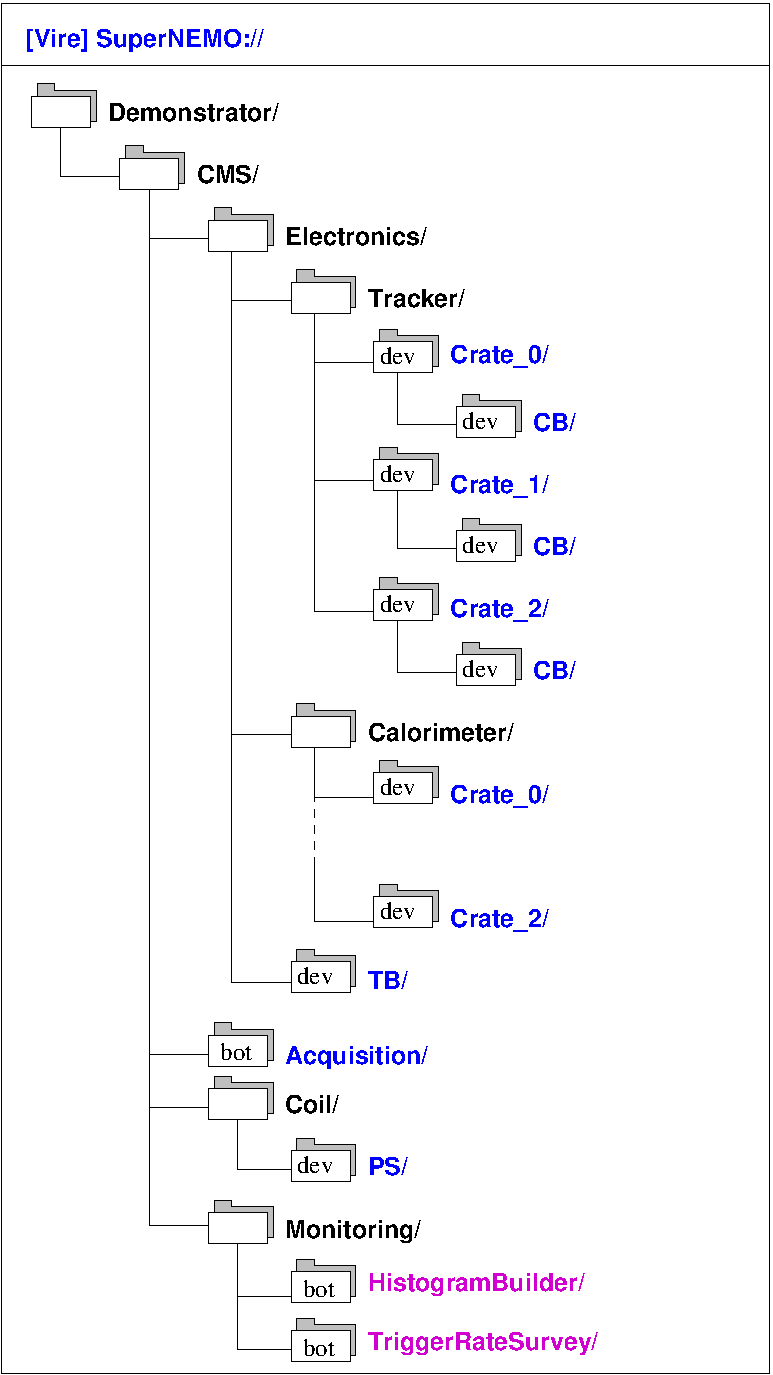
\includegraphics[width=5cm]{appendix/images/MOS_device_example_2.pdf}
\end{center}
\caption{Example of a hierarchy of  devices described by the Vire API.
  The root device is named  \texttt{SuperNEMO:}.  The top level (root)
  device  is  named  \texttt{Demonstrator}.  The  devices  colored  in
  \textcolor{blue}{blue}  are managed  through MOS/OPCUA.  The devices
  colored in \textcolor{magenta}{magenta} are directly embedded in the
  Vire server.  Devices with the \texttt{dev} tag are typical hardware
  device.  Devices  with the  \texttt{bot}  tag  are typical  software
  devices.   The  devices  colored in  \textbf{black}  are  structural
  pseudo-devices used to organize and  present a comprehensive view of
  the hierarchy. }\label{fig:an:mos_dev_2}
\end{figure}

The organisation of this hierarchy of devices is arbitrary and defined
by the designer of the  \emph{Control and Monitoring System}.  What is
important  to  understand  is  that  some  of  these  devices  can  be
associated  to  \emph{hardware  devices}  (a  power  supply  crate,  a
temperature probe\dots) and others  can be \emph{pseudo-devices}, i.e.
pure   software  object   (a   monitoring  robot,   a  file   transfer
daemon\dots).

In the context of the coupling of  the Vire server and the CMS server,
we are  in the event that  some devices are managed  by some MOS/OPCUA
servers and others are managed  in the Vire server itself.  Typically,
\emph{hardware devices}  are systematically managed through  the OPCUA
technology.  Vire has a mechanism to integrate such devices in its own
hierarchy.  This mechanism can  be considered like the \emph{mounting}
of   a   remote   filesystem   from  a   local   filesystem.    Figure
\ref{fig:an:mos_dev_0} illustrates  the case of many  hardware devices
-- managed by MOS -- that are integrated in the Vire system.  From the
Vire point of  view, the user does not see  the implementation details
for such  devices. He  does not  know the identity  of the  MOS server
hosting the device. He does not even know if the device is hosted by a
MOS server.  Devices are simply visible through the standard hierarchy
published by Vire with its  own device naming scheme, regardless their
true location.



\begin{figure}[h]
\begin{center}
\includegraphics[width=\linewidth]{appendix/images/MOS_device_example_0.pdf}
\end{center}
\caption{The  mounting of  many  MOS device  hierarchies  in the  Vire
  device hierarchy.  Each OPCUA server  runs a simple  hardware device
  that is \emph{mounted} from a specific node with its own path.
%% of  devices described by the Vire API.
%%   The root device is named  \texttt{SuperNEMO:}.  The top level (root)
%%   device is  named \texttt{Demonstrator}. The devices  colored in blue
%%   are managed  through MOS/OPCUA. The  devices colored in  magenta are
%%   directly embedded in the Vire server.  Devices with the \texttt{dev}
%%   tag are typical  hardware device. Devices with  the \texttt{bot} tag
%%   are typical software devices.
}\label{fig:an:mos_dev_0}
\end{figure}




\subsection{Example}

Using  the examples  displayed  in  figure \ref{fig:an:mos_dev_0},  we
consider  in detail  the way  one specific  device managed  by MOS  is
mounted   in  the   Vire   hierarchy.  Figure   \ref{fig:an:mos_dev_3}
illustrates the mounting of a MOS device in Vire.

Here the Vire  server publishes the path of a  device representing the
control board  of the third  electronic crate  for the tracker  of the
SuperNEMO demonstrator module.  The full Vire path of this device is:

\textcolor{blue}{\texttt{SuperNEMO://Demonstrator/CMS/Electronics/Tracker/Crate\_2/CB}}

This is  the only Vire identifier  recognized by user to  address this
device.

On    the   figure,    one    can   see    that    the   MOS    server
\texttt{lappc−f498l.in2p3.fr} (port 48904) hosts a simple device which
is locally named \texttt{ControlBoard}.

When  mounting   this  device  in   the  Vire  hierarchy,   the  local
\texttt{[CMS]}  namespace and  \texttt{ControlBoard} device  names are
hidden and replaced by the Vire device path.  All daughter devices and
datapoints of  the \texttt{CMS/ControlBoard} device are  integrated as
daughters        of        the         Vire        device        named\\
\texttt{SuperNEMO://Demonstrator/CMS/Electronics/Tracker/Crate\_2/CB}.


For example, the \texttt{FPGA\_main} daughter device is now associated
to the following Vire path:

\textcolor{blue}{\texttt{SuperNEMO://Demonstrator/CMS/Electronics/Tracker/Crate\_2/CB/FPGA\_main/}}

and  its  \texttt{Stop} method  is  automatically  addressed with  the
following \emph{leaf} path:

\textcolor{blue}{\texttt{SuperNEMO://Demonstrator/CMS/Electronics/Tracker/Crate\_2/CB/FPGA\_main/Stop}}


\begin{figure}[h]
\begin{center}
\includegraphics[width=0.8\linewidth]{appendix/images/MOS_device_example_3.pdf}
\end{center}
\caption{The  mounting of  one  MOS device and its local hierarchy  in the  Vire
  device hierarchy.}\label{fig:an:mos_dev_3}
\end{figure}



\subsection{Vire/MOS mapping}

As it can be  seen in the above example, the integration  of a new MOS
device in the Vire system is  achieved through soem kind of filesystem
mounting operation.   Particularly, it is  shown that the MOS  name of
the   mounted  root   device  is   replaced  by   an  arbitrary   Vire
path. However, all daughter  nodes (devices, datapoints) attached from
this root  node have their  relative MOS  names preserved in  the Vire
naming scheme.

Any  resource  (method)  associated  to any  of  such  daughter  nodes
inherits this relative naming scheme.

As Vire applications  describe resources through their  Vire paths, it
is thus needed to build an explicit map that associates resource paths
to MOS address  and name. The CMS  server will be able  to resolve the
MOS server/port and  embedded device associated to  the resource path.

The goal of the \texttt{devices\_launch.conf} file is not only to tell
the CMS server what MOS server should  be loaded and ran at start, but
also  to describe  the  \emph{mounting point/names}  used  by Vire  to
access the resources associated to MOS devices.  From the informations
stored in the  file, an explicit associative array must  be built when
the Vire server connect to the CMS server.  It will play the role of a
resource path resolver  when requests about resources will  be sent by
Vire applications.  This associative array  must be locked  during the
Vire/CMS connection.



%\subsubsection{Preparation of XML device models}

%% \noindent\underline{Pre-condition:}
%% The device is working and validated through the MOS/OPCUA server

%% \begin{enumerate}

%% \item Produce XML décrivant le modèle du device enrichi
%%   des metadata
%% Rédaction du fichier XML décrivant le modèle du device

%% \item Génération des fichiers model du type de device pour Vire

%% \item Génération des fichiers instances resolv.conf

%% \end{enumerate}


\vfill
\pagebreak
\clearpage

% end


\section{Vire messages}\label{app:vire_messages}

Within Vire  and between Vire  components and external  components, we
use  a communication  system  based on  Vire  messages.  This  section
describes the structure of such messages.

\subsection{General structure of a message}

Each message consists in two parts (figure \ref{fig-vire-message-message-cpp}):
\begin{itemize}

\item  the  \emph{header}  is   dedicated  to  generic  and  typicalle
  mandatory  informations  which  document   the  message  itself  and
  arbitrary high-level metadata.

\item  the \emph{body}  of the  message  contains the  real data: the payload.
  The structure of the message body depends on some convention. Vire uses
  its own convention to embed the payload data.

\end{itemize}

\begin{figure}[h]
\vskip 10pt
\small
\begin{Verbatim}[frame=single,xleftmargin=0.cm,label=\fbox{C++}]
struct vire::message::message {
  message_header header; // Header of the message
  message_body   body;   // Body of the message
};
\end{Verbatim}
\normalsize
\caption{The structure of a Vire message object (C++  class:
  \texttt{"vire::message::message"})}\label{fig-vire-message-message-cpp}
\end{figure}

\subsection{The message header}

The header contains (figure \ref{fig-vire-message-message_header-cpp}):
\begin{itemize}

  \item The mandatory \texttt{message\_id}  attribute is an identifier
    of the  message which  document the emitter  and a  unique message
    number.   Each emitter  is  responsible of  the  numbering of  the
    messages it  emits, typically using an  incremental technique. The
    message  number is  a positive  integer, starting  from 0  (figure
    \ref{fig-vire-message-message_identifier-cpp}).

  \item  The \texttt{timestamp}  attribute  encodes the  approximative
    time point when the message was  created. It contains the date and
    the time, using at least microsecond resolution.

    Typically,  with  JSON  encoding  system, it  is  expected  to  be
    formatted as a character string, using the following ISO format:

    \begin{center}
      \texttt{yyyymmddThhmmss.uuuuuu}
    \end{center}

    \noindent where:

    \vskip -10pt
    \begin{itemize}
    \item[\texttt{yyyymmdd} :] encodes year/month/day,
    \item[\texttt{hhmmssd} :] encodes hour/minute/second,
    \item[\texttt{uuuuuu} :] encodes microseconds.
    \end{itemize}

  \item   In   the   case    of   a   \emph{response}   message,   the
    \texttt{in\_reply\_to} attribute is set to identify the associated
    request message.

  \item  The \texttt{asynchronous}  boolean  attribute is  set if  the
    message processing  is explicitely requested  by the source  to be
    asynchronous (non-blocking).  In  RPC transactions, where requests
    are transmitted from one point to  the other, its default value is
    \emph{false}.   It  is possible  to  force  a RPC  transaction  in
    asynchronous mode.   This use  case is documented  elsewhere.  For
    event messaging, this flag is conventionally set to \emph{true}.

  \item  The  \texttt{body\_layout\_id}  attribute  is  the  mandatory
    identifier   of   the   layout   of  the   message   body   (class
    \texttt{"vire::utility::model\_identifier"}).  The  default layout
    for     message     body     inside    the     Vire     API     is
    \texttt{"vire::message::body\_format::typed\_payload"}, with version
    \texttt{"1.0"}                                             (figure
    \ref{fig-vire-utility-model_identifier-cpp}).

\end{itemize}


\begin{figure}[h]
\vskip 10pt
\small
\begin{Verbatim}[frame=single,xleftmargin=0.cm,label=\fbox{C++}]
struct vire::message::message_header {
  message_identifier message_id;     // Message identifier from the emitter.
  std::string        timestamp;      // Timestamp.
  message_identifier in_reply_to;    // Message identifier of the associated
                                     // request message (optional).
  bool               asynchronous,   // Asynchronous flag.
  vire::utility::model_identifier     body_layout_id; // Body layout identifier.
  std::map<std::string, std::string>  metadata;       // Key/value metadata dictionary.
};
\end{Verbatim}
\normalsize
\caption{The  structure  of  a   message  header  object  (C++  class:
  \texttt{"vire::message::message\_header"}).}\label{fig-vire-message-message_header-cpp}
\end{figure}

\begin{figure}[h]
\vskip 10pt
\small
\begin{Verbatim}[frame=single,xleftmargin=0.cm,label=\fbox{C++}]
struct vire::message::message_identifier {
  std::string emitter; // Name identifying the emitter of the message.
  int32_t     number;  // Number identifying the message in the emitter's
                       // message numbering scheme.
};
\end{Verbatim}
\normalsize
\caption{The      structure      of     a      message      identifier
  (C++  class:  \texttt{"vire::message::message\_identifier"}).}
\label{fig-vire-message-message_identifier-cpp}
\end{figure}

\begin{figure}[h]
\vskip 10pt
\small
\begin{Verbatim}[frame=single,xleftmargin=0.cm,label=\fbox{C++}]
struct vire::utility::model_identifier {
  std::string name;    // Name identifying the format of the message.
  std::string version; // String identifying the version of the format.
};
\end{Verbatim}
\normalsize
\caption{The structure of a model identifier (C++  class:  \texttt{"vire::utility::model\_identifier"}.}\label{fig-vire-utility-model_identifier-cpp}
\end{figure}




\begin{figure}[h]
\vskip 10pt
\small
\begin{Verbatim}[frame=single,xleftmargin=0.cm,label=\fbox{JSON}]
{
   "header" : {
      "message_id" : {
         "emitter" : "vire.server",
         "number" : 42
      },
      "timestamp" : "20160930T141408.413443",
      "in_reply_to" : {
         "initialized" : true,
         "value" : {
            "emitter" : "vire.client.0",
            "number" : 23
         }
      },
      "asynchronous" : false,
      "body_layout_id" : {
         "name" : "vire::message::body_format::typed_payload",
         "version" : {
            "initialized" : true,
            "value" : "1.0"
         }
      },
      "metadata" : [
         {
            "key" : "key1",
            "value" : "foo"
         },
         {
            "key" : "key2",
            "value" : "42"
         },
         {
            "key" : "key3",
            "value" : "3.1415899999999999"
         },
         {
            "key" : "key4",
            "value" : "true"
         }
      ]
   }
  "body" : {
      ...
   }
}
\end{Verbatim}
\normalsize
\caption{Example of  a   message  header  object in JSON format.}
\label{fig-vire-message-message_header-json}
\end{figure}

\vfill
\clearpage
\pagebreak

\subsection{The message body}

The    default    message   body    layout    in    Vire   is    named
\texttt{"vire::message::body\_format::typed\_payload"}        (version
\texttt{"1.0"}).   Each  message used  within  the  Vire framework  is
supposed to use this layout.  The general idea is that the body of the
message embeded the  \emph{payload object} that has  to be transmitted
between  two components  of  the system.   \emph{Payload objects}  are
classified in one of the three following categories:

\begin{enumerate}

\item \emph{Request}:  describes a request submitted  by one component
  to another component (generally during a synchronous RPC transaction).

\item  \emph{Response}: describes  the  response to  a former  request
  (generally during a synchronous RPC transaction).

\item \emph{Event}: describes an  arbitrary information record (alarm,
  exception, signal\dots) which is transmitted asynchronously.

\end{enumerate}

Vire implements the following class hierarchy:

\begin{center}
\begin{tikzpicture}
  \node (payload)  at (0,2)  [draw] {\texttt{vire::utility::base\_payload}};
  \node (request)  at (-4,0) [draw] {\texttt{vire::utility::base\_request}};
  \node (response) at (2,0)  [draw] {\texttt{vire::utility::base\_response}};
  \node (event)    at (8,0)  [draw] {\texttt{vire::utility::base\_event}};

  %\draw[style=help lines] (-3,-1) grid (10,4);
  \draw (node cs:name=response,anchor=north) |- (0,1);
  \draw (node cs:name=event,anchor=north)    |- (0,1);
  \draw[->] (node cs:name=request,anchor=north)
  |- (0,1) -| (node cs:name=payload,anchor=south);
\end{tikzpicture}
\end{center}

The requirements for the transmitted object are the following:

\begin{itemize}

\item The  type of the object  must be conventionally associated  to a
  unique     \emph{model      identifier}     object      (see     the
  \texttt{"vire::utility::model\_identifier"} class)  which contains a
  unique   name   (\textit{string    identifier})   and   possibly   a
  \textit{version identifier}.  Each software  component that may send
  or  receive the  object  should agree  on  this type  identification
  scheme.   This   enable  the  use  of   object  factories,  whatever
  programming  langage  is used  on  both  side of  the  communication
  system.

\item  For each  software component,  the object  type must  have some
  dedicated  encoding/decoding  functions  available  (again  whatever
  programming language is used). For example the Vire API supports the
  following encoding formats:

  \begin{itemize}

  \item JSON (MIME  encoding type: \texttt{"application/x-json"}), which
    is supportable by many languages,

  \item  Protobuf  (Google  Protocol   Buffers,  MIME  encoding  type:
    \texttt{"application/x-protobuf"}), which is also widely supported,

  \item   Boost/serialisation   (XML,    text   or   binary   archives
    \texttt{"application/x-boost-serialization-xml"},
    \texttt{"application/x-boost-serialization-text"},
    \texttt{"application/x-boost-serialization-binary"}),    which    in
    principle is supported by C++ only.

  \end{itemize}

  The Protobuf  encoding format will be  used to serialize/deserialize
  the  Vire  messages transported  between  the  Vire server  and  the
  CMS/LAPP server.

\end{itemize}

Vire uses a dedicated layout to represent the body of any message with
its embedded payload object. With this technique, the structure of the
body          contains         two          attributes         (figure
\ref{fig-app-vire-message-message_body-cpp}):

\begin{enumerate}

\item The \texttt{payload\_type\_id} specifies the type of the payload
  object   (figure   \ref{fig-app-vire-utility-model_identifier-cpp}).
  This unique name  is conventionaly fixed for a  given application. A
  version tag allows to support possible evolution of the object type.

\item The  \texttt{payload} is a  handle to  a payload object  of type
  request, response or event.

  %% \begin{itemize}
  %% \item Within  the producer  component of  the message,  the encoding
  %%   function associated to the object  type is responsible to generate
  %%   the JSON stream for the object and store it in the buffer.

  %% \item Within  the consumer  component of  the message,  the decoding
  %%   function associated to the object type is responsible to parse the
  %%   JSON stream stored in the buffer and restore the object in memory.

  %% \end{itemize}

  It is expected  that, on both sides of the  connection, the software
  components can  access dedicated  software plugins which  ensure the
  support  of  various   \emph{payload  object  types}  conventionnaly
  associated  with  their  \emph{payload type  identifiers}  and  also
  providing JSON and/or Protobuf encoding/decoding functionalities.

  %% The   system  allows  to  support
  %% modification  in the  structure of  the objects  thanks to  version
  %% tagging.

\end{enumerate}

\begin{figure}[h]
\vskip 10pt
\small
\begin{Verbatim}[frame=single,xleftmargin=0.cm,label=\fbox{C++}]
struct message_body {
  vire::utility::model_identifier     payload_type_id; // Object type identifier.
  const vire::utility::base_payload * payload;         // Handle to a payload object.
};
\end{Verbatim}
\normalsize
\caption{The structure of a message body object (C++).}
\label{fig-app-vire-message-message_body-cpp}
\end{figure}

\begin{figure}[h]
\vskip 10pt
\small
\begin{Verbatim}[frame=single,xleftmargin=0.cm,label=\fbox{JSON}]
{
  "header" : {
    ...
  },
  "body" : {
    "payload_type_id" : {
      "name" : "vire::message::testing::error_event",
      "version" : {
        "initialized" : false
      }
    },
    "payload" : {
      "timestamp" : "20160930T141743.759085"
      "err" : {
        "code" : 3,
        "message" : "A basic error"
      },
    }
  }
}
\end{Verbatim}
\normalsize
\caption{Example of  a   message  body  object in JSON format.}
\label{fig-vire-message-message_body-json}
\end{figure}

\vfill
\clearpage
\pagebreak

% end

%\input{appendix/app_json_fmt.tex}

\section{The \emph{Protocol Buffers} format}\label{app:protobuf_fmt}

\subsection{Introduction}

The  Google  Protocol Buffers  (\emph{protobuf})  library  is used  to
represent the objects that are exchanged between the Vire clients, the
Vire server and the CMS server.  The  version 3 of the format is used,
implying   at   least   version   3.0.0  (September   2016)   of   the
\emph{protobuf} library.

Each  data   structure  of  interest   can  be  described   through  a
\texttt{.proto}  file  from  which  stub files  can  be  automatically
generated  with the  \texttt{protoc} compiler.  For Vire  and its  CMS
interface, the C++ and Java programming languages will be used.


A  collection of  \texttt{.proto}  files are  provided  with the  Vire
library to represent all kind  of data structures transferable between
networked agents  (Vire server,  Vire clients, CMS/LAPP  server).  The
objects of  the highest level  are named \emph{payload  objects} (like
\emph{request},  \emph{response} and  \emph{event} objects).   They
are composed of attributes of more basic data structures.

\subsection{Example}

The following  class diagram  illustrates two data  structures defined
within the Vire library with an inheritance relationship between them.

\begin{center}
  \begin{tikzpicture}
    \node (base)     at (0,1.5)  [draw] {\texttt{vire::utility::base\_error}};
    \node (setup)    at (0,0)  [draw] {\texttt{vire::utility::invalid\_setup\_id\_error}};

    \draw[->]   (node cs:name=setup,anchor=north) |- (0,1);
    |- (0,1) -| (node cs:name=base,anchor=south);
  \end{tikzpicture}
\end{center}

The \texttt{vire::utility::base\_error}  is the  parent class  for all
\emph{error}  objects.   It  contains   two  attributes:   an  integer
\emph{error code}  and a  character string describing  the \emph{error
  message}.

The   \texttt{vire::utility::invalid\_setup\_id\_error}  class   is  a
specialized error class  which represents explicitely an  error due to
an identification  failure of  the experimental setup.   It implements
additional mutually exclusive attributes: the \emph{unrecognized name}
of the setup or the \emph{unrecognized version} of the setup.

This   example  illustrates   the  protobuf   representation  of   the
\texttt{vire::utility::base\_error}  in the  Vire  library, using  the
\texttt{"vire/utility/BaseError.proto"} file:

\small
\begin{Verbatim}[frame=single,xleftmargin=0.cm,label=\fbox{protobuf}]
  syntax = "proto3";
  package vire.utility; // Namespace

  message BaseError {

    // reserved 1; // Reserved for _base message

    // Attributes:
    int32  code           = 100; // The error code
    string message_format = 101; // The error description message

  }
\end{Verbatim}
\normalsize

\vfill
\clearpage
\pagebreak

\subsection{Vire protobuf conventions}

Vire uses the following conventions:

\begin{enumerate}

\item
  The member index  \texttt{1} is reserved to represent the  link of a
  class to its main base/parent class (if any).  It is not used if the
  data structure does not inherit any data structure.
  If a data structure naturally inherits another one, it is thus possible
  to  represent the  inheritance  relationship as  illustrated with  the
  \texttt{"vire/utility/InvalidSetupIdError.proto"}      file      which
  represents the \texttt{vire::utility::invalid\_setup\_id\_error} class
  in the Vire library:

  \small
  \begin{Verbatim}[frame=single,xleftmargin=0.cm,label=\fbox{protobuf}]
    syntax = "proto3";
    package vire.utility; // Namespace

    import "vire/utility/BaseError.proto"; // Dependency

    message InvalidSetupIdError {

      BaseError _base = 1; // The base class

      // Additional attributes:
      oneof detail { // Mutual exclusion
        string invalid_setup_name    = 100; // The failed setup name
        string invalid_setup_version = 101; // The failed setup version
      }

    }
  \end{Verbatim}
  \normalsize

\item The  \texttt{\_base} member  is conventionally  used to  represent the
  inheritance   relationship    from   a   data   structure    of   type
  \texttt{"vire.utility.BaseError"}.

\item Member indexes from \texttt{2}  to \texttt{99} are also reserved
  for possible future usage (multiple inheritance, metadata\dots).

\item
  The first member of the data structure must start at index \texttt{100}.

\end{enumerate}

\vfill
\clearpage
\pagebreak

% end


\section{Vire payload objects}\label{app:payload}

\subsection{Introduction}

As  mentioned in  appendix \ref{app:protobuf_fmt},  Vire messages  are
wrappers for \emph{payload objects}.  Each  type of payload object can
be represented  through the \emph{protobuf} mechanism.   The following
class hierarchy shows the base architecture used to define new payload
objects.

\begin{center}
\begin{tikzpicture}
  \node (payload)  at (0,2)   [draw] {\texttt{vire::utility::base\_payload}};
  \node (request)  at (-4,0)  [draw] {\texttt{vire::utility::base\_request}};
  \node (response) at (2,0)   [draw] {\texttt{vire::utility::base\_response}};
  \node (event)    at (8,0)   [draw] {\texttt{vire::utility::base\_event}};
  \node (my)       at (-4,-2) [draw] {\texttt{my\_request}};
  \node (your)     at (2,-2)  [draw] {\texttt{your\_response}};
  \node (its)    at (8,-2)    [draw] {\texttt{its\_alarm}};

  %\draw[style=help lines] (-6,-2) grid (10,2);
  \draw (node cs:name=response,anchor=north) |- (0,1);
  \draw (node cs:name=event,anchor=north)    |- (0,1);
  \draw[->] (node cs:name=request,anchor=north)
  |- (0,1) -| (node cs:name=payload,anchor=south);
  \draw[->] (node cs:name=my,anchor=north)
  |- (-4,-1) -| (node cs:name=request,anchor=south);
  \draw[->] (node cs:name=your,anchor=north)
  |- (2,-1) -| (node cs:name=response,anchor=south);
  \draw[->] (node cs:name=its,anchor=north)
  |- (8,-1) -| (node cs:name=event,anchor=south);
\end{tikzpicture}
\end{center}


\begin{center}
\vskip 10pt
\small
\begin{tabular}{|l|l|l|}
  \hline
  \textbf{Vire C++ class} & \textbf{protobuf message type} & \textbf{protobuf definition file} \\
  \hline
  \hline
  \multicolumn{3}{|c|}{\emph{general types}} \\
  \hline
  boost::posix\_time::ptime & google.protobuf.Timestamp & google/protobuf/timestamp.proto \\
  \hline
  \hline
  \multicolumn{3}{|c|}{\emph{identifier types}} \\
  \hline
  vire::utility::base\_identifier & vire.utility.Baseidentifier & vire/utility/Baseidentifier.proto \\
  \hline
  vire::utility::instance\_identifier & vire.utility.InstanceIdentifier & vire/utility/InstanceIdentifier.proto \\
  \hline
  vire::utility::model\_identifier & vire.utility.ModelIdentifier & vire/utility/ModelIdentifier.proto \\
  \hline
  \hline
  \multicolumn{3}{|c|}{\emph{error types}} \\
  \hline
  vire::utility::base\_error & vire.utility.BaseError & vire/utility/BaseError.proto \\
  \hline
  vire::utility::invalid\_context\_error & vire.utility.InvalidContextError & vire/utility/InvalidContextError.proto \\
  \hline
  vire::utility::invalid\_setup\_id\_error & vire.utility.InvalidSetupIdError & vire/utility/InvalidSetupIdError.proto \\
  \hline
  \hline
  \multicolumn{3}{|c|}{\emph{payload types}} \\
  \hline
  vire::utility::base\_payload & vire.utility.BasePayload & vire/utility/BasePayload.proto \\
  \hline
  vire::utility::base\_request & vire.utility.BaseRequest & vire/utility/BaseRequest.proto \\
  \hline
  vire::utility::base\_response & vire.utility.BaseResponse & vire/utility/BaseResponse.proto \\
  \hline
  vire::utility::base\_event & vire.utility.BaseEvent & vire/utility/BaseEvent.proto \\
  \hline
  vire::utility::base\_alarm & vire.utility.BaseAlarm & vire/utility/BaseAlarm.proto \\
  \hline
  \hline
  \multicolumn{3}{|c|}{\emph{messenging types}} \\
  \hline
  vire::message::message\_identifier & vire.message.MessageIdentifier & vire/message/MessageIdentifier.proto \\
  \hline
  vire::message::msg\_header & vire.message.MsgHeader & vire/message/MsgHeader.proto \\
  \hline
  vire::message::msg\_body & vire.message.MsgBody & vire/message/MsgBody.proto \\
  \hline
  vire::message::message & vire.message.Message & vire/message/Message.proto \\
  \hline
\end{tabular}
\normalsize
\end{center}


\begin{center}
\vskip 10pt
\small
\begin{tabular}{|l|l|l|}
  \hline
  \multicolumn{3}{|c|}{\emph{Resource management related types}} \\
  \hline
  vire::cms::resource\_status\_record & vire.cms.ResourceStatusRecord & vire/cms/ResourceStatusRecord.proto \\
  \hline
  vire::cms::resource\_fetch\_status\_request & vire.cms.ResourceFetchStatusRequest & vire/cms/ResourceFetchStatusRequest.proto \\
  \hline
  vire::cms::resource\_fetch\_status\_success\_response & vire.cms.ResourceFetchStatusSuccessResponse & vire/cms/ResourceFetchStatusSuccessResponse.proto \\
  \hline
  vire::cms::resource\_fetch\_status\_failure\_response & vire.cms.ResourceFetchStatusFailureResponse & vire/cms/ResourceFetchStatusFailureResponse.proto \\
  \hline
  vire::cms::resource\_exec\_request & vire.cms.ResourceExecRequest & vire/cms/ResourceExecRequest.proto \\
  \hline
  vire::cms::resource\_exec\_success\_response & vire.cms.ResourceExecSuccessResponse & vire/cms/ResourceExecSuccessResponse.proto \\
  \hline
  vire::cms::resource\_exec\_failure\_response & vire.cms.ResourceExecFailureResponse & vire/cms/ResourceExecFailureResponse.proto \\
  \hline
  vire::cms::resource\_exec\_non\_blocking\_request & vire.cms.ResourceExecNonBlockingRequest & vire/cms/ResourceExecNonBlockingRequest.proto \\
  \hline
  vire::cms::resource\_exec\_non\_blocking\_ack\_response & vire.cms.ResourceExecNonBlockingAckResponse & vire/cms/ResourceExecNonBlockingAckResponse.proto \\
  \hline
  vire::cms::resource\_exec\_non\_blocking\_noack\_response & vire.cms.ResourceExecNonBlockingNoackResponse & vire/cms/ResourceExecNonBlockingNoackResponse.proto \\
  \hline
  vire::cms::resource\_exec\_non\_blocking\_success\_event & vire.cms.ResourceExecNonBlockingSuccessEvent & vire/cms/ResourceExecNonBlockingSuccessEvent.proto \\
  \hline
  vire::cms::resource\_exec\_non\_blocking\_failure\_event & vire.cms.ResourceExecNonBlockingFailureEvent & vire/cms/ResourceExecNonBlockingFailureEvent.proto \\
  \hline
  vire::cms::resource\_exec\_error & vire.cms.ResourceExecError & vire/cms/ResourceExecError.proto \\
  \hline
  vire::cms::invalid\_status\_error & vire.cms.ResourceExecError & vire/cms/ResourceExecError.proto \\
  \hline
  %% vire::cms::invalid\_credentials\_error & vire.cms.InvalidCredentialsError & vire/cms/InvalidCredentialsError.proto \\
  %% \hline
  %% vire::cms::invalid\_user\_error & vire.cms.InvalidUserError & vire/cms/InvalidUserError.proto \\
  %% \hline
  vire::cms::invalid\_resource\_error & vire.cms.InvalidUserError & vire/cms/InvalidUserError.proto \\
  \hline
  vire::cms::no\_pubsub\_resource\_error & vire.cms.NoPubsubResourceError & vire/cms/NoPubsubResourceError.proto \\
  \hline
  \hline
  \multicolumn{3}{|c|}{\emph{Resource pub/sub management types}} \\
  \hline
  vire::cms::resource\_pubsub\_subscribe\_request & vire.cms.ResourcePubsubSubscribeRequest & vire/cms/ResourcePubsubSubscribeRequest.proto \\
  \hline
  vire::cms::resource\_pubsub\_subscribe\_success\_response & vire.cms.ResourcePubsubSubscribeRSuccessResponse & vire/cms/ResourcePubsubSubscribeRSuccessResponse.proto \\
  \hline
  vire::cms::resource\_pubsub\_subscribe\_failure\_response & vire.cms.ResourcePubsubSubscribeRFailureResponse & vire/cms/ResourcePubsubSubscribeRSuccessResponse.proto \\
  \hline
  \hline
  \multicolumn{3}{|c|}{\emph{Vire/CMS server interface types}} \\
  \hline
  vire::cmsinterface::connection\_request & vire.cmsinterface.ConnectionRequest & vire/cmsinterface/ConnectionRequest.proto \\
  \hline
  vire::cmsinterface::connection\_success\_response & vire.cmsinterface.ConnectionSuccessResponse & vire/cmsinterface/ConnectionSuccessResponse.proto \\
  \hline
  vire::cmsinterface::connection\_failure\_response & vire.cmsinterface.ConnectionFailureResponse & vire/cmsinterface/ConnectionFailureResponse.proto \\
  \emph{embedded:} unknown\_resources\_error & .UnknownResourcesError &  \\
  \hline
  vire::cmsinterface::disconnection\_request & vire.cmsinterface.DisconnectionRequest & vire/cmsinterface/DisconnectionRequest.proto \\
  \hline
  vire::cmsinterface::disconnection\_success\_response & vire.cmsinterface.DisconnectionSuccessResponse & vire/cmsinterface/DisconnectionSuccessResponse.proto \\
  \hline
  %% \hline
  %% vire::cmsinterface::disconnection\_failure\_response & vire.cmsinterface.DisconnectionFailureResponse & vire/cmsinterface/DisconnectionFailureResponse.proto \\
\end{tabular}
\normalsize
\end{center}

\subsection{Basic data structures}

Any  payload object  (request, response  or event)  generally contains
some information records which are  specific to the functionalities of
the  payload  object they  belong.   These  records are  of  arbitrary
types. Of course they should be  translatable in terms of the protobuf
library.
%Of course they can be (de)serialized using JSON.
Some of these types are very  general and defined within the Vire core
API itself because they are reused by various payload objects not only
through  the Vire-CMS/LAPP  interface  but also  between  Vire clients  and
servers, independently  of the  CMS/LAPP server.  However,  the use  of the
Protocol Buffers interface makes possible  to publish the interface of
such data to the outside world, including the CMS/LAPP server in priority.

%% Other one are specific to the Vire/CMS interface and thus managed only
%% in the \texttt{Vire\_CMSInterface} API.
These  types  are considered  as  \emph{basic}.  Among them  we  find:
generic error  types, generic  identifier types,  timestamps, resource
status records\dots We propose to describe them in this section.

Once a sufficient collection of  basic data record types is available,
it  is possible  to describe  high  level payload  object types  which
aggregate attributes of such types.

Other record  types are specific to  some payload objects and  will be
never  used outside  the scope  of these  payload objects.   Such data
structures will be  explicitely declared with the  payload object they
belong to, likely as embedded types/classes.


\subsubsection{Errors}

Some  \emph{response} or  \emph{event} payload  objects may  contain a
specific  error  record  object.   A  \emph{failure  response}  or  an
\emph{exception  event}  object will  generally  embed  such an  error
record object.

Each  \emph{error record}  is represented  by an  instance of  a given
error type.   Each of  the error  types defined  in Vire  inherits the
\texttt{vire::utility::base\_error}      base       class      (figure
\ref{fig-app-payload-base_error})   which   contains   the   following
attributes:

\begin{itemize}

\item the error code: A non zero  integer which is set to 1 by default
  (indicating  a  generic  failure  case).   The  error  code  can  be
  conventionally  set to  any positive  integer value  to represent  a
  specific error case, depending on the context.

\item the error  message: an optional human  readable character string
  which documents the error as usefully as possible.

\end{itemize}

\begin{figure}[h]
\vskip 10pt
\small
\begin{Verbatim}[frame=single,xleftmargin=0.cm,label=\fbox{C++}]
struct vire::utility::base_error
{
  // Attributes:
  int         code;           // Error code (>0).
  std::string message_format; // Error message (optional).
};
\end{Verbatim}
\normalsize
\caption{The structure of a \texttt{"vire::utility::base\_error"} object
  (C++).}
\label{fig-app-payload-base_error}
\end{figure}


%% An example of JSON formatted basic error object is given in figure
%% \ref{fig-app-payload-base_error-1}.
%%
%% \begin{figure}[h]
%% \vskip 10pt
%% \small
%% \begin{Verbatim}[frame=single,xleftmargin=0.cm,label=\fbox{\texttt{JSON}}]
%% {
%%   "code" : "42",
%%   "message_format" : "Invalid AMQP server port=[2341]"
%% }
%% \end{Verbatim}
%% \normalsize
%% \caption{JSON  formatted  basic  error  object  (class
%%   \texttt{vire::utility::base\_error}.}
%% \label{fig-app-payload-base_error-1}
%% \end{figure}

Several type of generic errors are defined in Vire:


\begin{center}
\begin{tikzpicture}
  \node (base)     at (0,2)  [draw] {\texttt{vire::utility::base\_error}};
  \node (context)  at (-4,0) [draw] {\texttt{vire::utility::invalid\_context\_error}};
  \node (setup)    at (0,-1)  [draw] {\texttt{vire::utility::invalid\_setup\_id\_error}};
  \node (resource) at (4,0)  [draw] {\texttt{vire::cms::invalid\_resource\_error}};
  \node (user)     at (8,-1)  [draw] {\texttt{vire::cms::invalid\_user\_error}};

  \draw     (node cs:name=setup,anchor=north)    |- (0,1);
  \draw     (node cs:name=resource,anchor=north) |- (0,1);
  \draw     (node cs:name=user,anchor=north)     |- (0,1);
  \draw[->] (node cs:name=context,anchor=north)
  |- (0,1) -| (node cs:name=base,anchor=south);
\end{tikzpicture}
\end{center}

\noindent
Here are a few error object types defined in Vire.  Some types belongs
to the \texttt{utility} namespace, other  ones are in the \texttt{cms}
namespace:

\begin{itemize}

\item \texttt{"vire::utility::invalid\_context\_error"} : occurs typically when
  the general context of the execution of a given resource is not adapted.\\
  It is mapped to the \texttt{"vire.utility.InvalidContextError"} protobuf record.

\item \texttt{"vire::utility::invalid\_setup\_id\_error"} : occurs in case
  of an invalid identification of the experimental setup managed
  by the Vire or CMS server.\\
  It is mapped to the \texttt{"vire.utility.InvalidSetupIdError"} protobuf record.

\item \texttt{"vire::cms::invalid\_resource\_error"} : occurs in case
  of an invalid identification of a resource.\\
  It is mapped to the  \texttt{"vire.cms.InvalidResourceError"} protobuf record.

\item \texttt{"vire::cms::invalid\_status\_error"}: occurs when an attempt
  to access a resource that has not the proper status.\\
  It is mapped to the  \texttt{"vire.cms.InvalidStatusError"} protobuf record.

\item \texttt{"vire::cms::invalid\_user\_error"} : occurs in case
  of an invalid identification of an user.\\
  It is mapped to the  \texttt{"vire.cms.InvalidUserError"} protobuf record.

\item \texttt{"vire::cms::invalid\_credentials\_error"} : occurs in case
  of user authentication error.\\
  It is mapped to the  \texttt{"vire.cms.InvalidCredentialsError"} protobuf record.

\item \texttt{"vire::cms::resource\_exec\_error"} : occurs in case
  of error at the execution of a given resource.\\
  It is mapped to the  \texttt{"vire.cms.ResourceExecError"} protobuf record.

\end{itemize}



\subsubsection{Object and type identifiers}

Vire  uses  some dedicated  classes  to  represent the  identifier  of
various objects  (or \emph{instances})  as well  as various  types (or
\emph{models})  of components.  Vire  implements  the following  class
hierarchy:

\begin{center}
\begin{tikzpicture}
  \node (base)  at (0,2)  [draw] {\texttt{vire::utility::base\_identifier}};
  \node (instance)  at (-4,0) [draw] {\texttt{vire::utility::instance\_identifier}};
  \node (model) at (4,0)  [draw] {\texttt{vire::utility::model\_identifier}};

  \draw (node cs:name=model,anchor=north) |- (0,1);
\draw[->] (node cs:name=instance,anchor=north)
  |- (0,1) -| (node cs:name=base,anchor=south);
\end{tikzpicture}
\end{center}

The          \texttt{vire::utility::base\_identifier}          (figure
\ref{fig-app-payload-base_identifier}) class is  a pure abstract class
that cannot be instantiated. However  it contains a mandatory name and
an  optional  version description  which  are  used by  all  inherited
classes:

\begin{itemize}

\item The   \texttt{vire::utility::instance\_identifier}    concrete   class
inherits  \texttt{vire::utility::base\_identifier}  and   is  used  to
identify \underline{unique instances of objects} known by the system.

\item The  \texttt{vire::utility::model\_identifier}   concrete  class  also
inherits  \texttt{vire::utility::base\_identifier}  and   is  used  to
identify \underline{types of objects} registered in the system.

\end{itemize}

The only difference between these two classes is the validation scheme
of  the name  attribute.

\begin{figure}[h]
\vskip 10pt
\small
\begin{Verbatim}[frame=single,xleftmargin=0.cm,label=\fbox{C++}]
struct base_identifier
{
  // Attributes:
  std::string name;    // The mandatory name uniquely identifying the object or
                       // the type of object.
  std::string version; // An optional character string representing the version
                       // of the object type.
};
\end{Verbatim}
\normalsize
\caption{The structure of the \texttt{vire::utility::base\_identifier}
  class (C++).}
\label{fig-app-payload-base_identifier}
\end{figure}

%%  Figure  \ref{fig-app-payload-identifier-json}
%% shows an example of instance indentifier.
%% \begin{figure}[h]
%% \vskip 10pt
%% \small
%% \begin{Verbatim}[frame=single,xleftmargin=0.cm,label=\fbox{\texttt{JSON}}]
%% {
%%   "name" : "vire::resource::invalid_resource_error",
%%   "version" : "1.0"
%% }
%% \end{Verbatim}
%% \normalsize
%% \caption{JSON  formatted class identifier  object (class
%%   \texttt{vire::utility::model\_identifier}).   Here one  identifies a
%%   specific error type.}
%% \label{fig-app-payload-identifier-json}
%% \end{figure}


\vfill
\pagebreak
\clearpage

\subsubsection{Resource related objects}

\begin{itemize}

\item
Class \texttt{vire::cms::invalid\_resource\_error} (figure \ref{fig-app-payload-invalid_resource_error}).

\begin{center}
\begin{tikzpicture}
  \node (base)  at (0,2)  [draw] {\texttt{vire::utility::base\_error}};
  \node (ire)  at (0,0) [draw] {\texttt{vire::cms::invalid\_resource\_error}};
  \draw[->] (node cs:name=ire,anchor=north)
  |- (0,1) -| (node cs:name=base,anchor=south);
\end{tikzpicture}
\end{center}

\begin{figure}[h]
\vskip 10pt
\small
\begin{Verbatim}[frame=single,xleftmargin=0.cm,label=\fbox{C++}]
struct vire::cms::invalid_resource_error : public vire::utility::base_error
{
  // Attributes:
  std::string invalid_resource_path; // Invalid resource path
  std::string invalid_resource_id;   // Invalid resource internal ID (Vire server only)
};
\end{Verbatim}
\normalsize
\caption{The structure  of a invalid resource error object (C++).}
\label{fig-app-payload-invalid_resource_error}
\end{figure}

\begin{figure}[h]
\vskip 10pt
\small
\begin{Verbatim}[frame=single,xleftmargin=0.cm,label=\fbox{JSON++}]
{
  "code" : "3",
  "message_format" : "Resource path 'Atlas://Calorimeter/HV/Crate1/stop' is invalid",
  "invalid_resource_path" : "Atlas://Calorimeter/HV/Crate1/stop"
}
\end{Verbatim}
\normalsize
\caption{JSON formatted invalid resource error object.}
\label{fig-app-payload-invalid_resource_error-json}
\end{figure}


\item
Class     \texttt{vire::cms::resource\_status\_record}    (figure
\ref{fig-app-payload-resource_status_record}).

\end{itemize}

\begin{figure}[h]
\vskip 10pt
\small
\begin{Verbatim}[frame=single,xleftmargin=0.cm,label=\fbox{C++}]
struct vire::cms::resource_status_record
{
  // Attributes:
  std::string path;      // Path of the resource
  std::string timestamp; // Timestamp of the last modification
  uint16_t    flags;     // Status bits (Missing/Disabled/Pending/Error)
};
\end{Verbatim}
\normalsize
\caption{The structure  of a resource status record object (C++).}
\label{fig-app-payload-resource_status_record}
\end{figure}


\begin{figure}[h]
\vskip 10pt
\small
\begin{Verbatim}[frame=single,xleftmargin=0.cm,label=\fbox{JSON}]
{
  "path" : "SuperNEMO://Demonstrator/CMS/Coil/Control/Current/__dp_read__",
  "timestamp" : "20160612T212432.324517",
  "flags" : 2
}
\end{Verbatim}
\normalsize
\caption{JSON formatted resource status record object.}
\label{fig-app-payload-resource_status_record-json}
\end{figure}

\vfill
\pagebreak
\clearpage

\subsection{Connection of the Vire server to the CMS server}


\begin{itemize}

\item   The   \texttt{vire::cmslapp::connection\_request}   class
  (version \texttt{1.0})  represents a connection request  sent by the
  Vire server to the  CMS server through the \textcolor{blue}{service}
  channel.

\begin{center}
\begin{tikzpicture}
  \node (base)  at (0,2)  [draw] {\texttt{vire::utility::base\_request}};
  \node (cr)  at (0,0) [draw] {\texttt{vire::cmslapp::connection\_request}};
  \draw[->] (node cs:name=cr,anchor=north)
  |- (0,1) -| (node cs:name=base,anchor=south);
\end{tikzpicture}
\end{center}

\noindent Class registration:
\begin{itemize}
\item name: \texttt{"vire::cmslapp::connection\_request"}
\item version: "1.0"
\end{itemize}

\begin{figure}[h]
\vskip 10pt
\small
\begin{Verbatim}[frame=single,xleftmargin=0.cm,label=\fbox{C++}]
struct vire::cmslapp::connection_request : public vire::utility::base_request
{
  // Attributes:
  vire::utility::instance_identifier  setup_id; // Identifier of the experimental setup
  std::vector<std::string> requested_resources; // The list of requested resources
                                                // addressed by path
};
\end{Verbatim}
\normalsize
\caption{The structure of the connection  request object to be emitted
  by the Vire server to the CMS server (C++).}
\label{fig-app-payload-connection_request}
\end{figure}

\begin{figure}[h]
\vskip 10pt
\small
\begin{Verbatim}[frame=single,xleftmargin=0.cm,label=\fbox{JSON}]
{
  "setup_id" : {
    "name" : "snemo",
    "version" : "1.0.2"
  },
  "requested_resources" : [
    "SuperNEMO://Demonstrator/CMS/Coil/PS/Control/Current/__dp_read__",
    "SuperNEMO://Demonstrator/CMS/Coil/PS/Control/Current/__dp_write__",
    ...
    "SuperNEMO://Demonstrator/CMS/Acquisition/start",
    "SuperNEMO://Demonstrator/CMS/Acquisition/stop"
  ]
}
\end{Verbatim}
\normalsize
\caption{A JSON formatted  connection request object sent  by the Vire
  server to the CMS server (C++).}
\label{fig-app-payload-connection_request-json}
\end{figure}


\item  The  \texttt{vire::cmslapp::connection\_success\_response}
  class represents  the response sent back  to the Vire server  by the
  CMS server through the  \textcolor{blue}{service} channel in case of
  success.

\begin{center}
\begin{tikzpicture}
  \node (base)  at (0,2)  [draw] {\texttt{vire::utility::base\_response}};
  \node (csr)  at (0,0) [draw] {\texttt{vire::cmslapp::connection\_success\_response}};
  \draw[->] (node cs:name=csr,anchor=north)
  |- (0,1) -| (node cs:name=base,anchor=south);
\end{tikzpicture}
\end{center}

\noindent Class registration:
\begin{itemize}
\item name: \texttt{"vire::cmslapp::connection\_success\_response"}
\item version: "1.0"
\end{itemize}

\begin{figure}[h]
\vskip 10pt
\small
\begin{Verbatim}[frame=single,xleftmargin=0.cm,label=\fbox{C++}]
struct connection_success_response
  : public vire::utility::base_response
{
  typedef vire::resource::resource_status_record resource_status_record; // Type alias

  // Attributes:
  std::vector<resource_status_record> resources_snapshot; // Requested resources snapshot
};
\end{Verbatim}
\normalsize
\caption{The structure  of the connection success  response emitted by
  the CMS server to the Vire server (C++).}
\label{fig-app-payload-connection_success_response}
\end{figure}



\begin{figure}[h]
\vskip 10pt
\small
\begin{Verbatim}[frame=single,xleftmargin=0.cm,label=\fbox{\texttt{JSON}}]
{
  "resources_snapshot"  : [
    {
      "path" : "SuperNEMO://Demonstrator/CMS/Coil/PS/Control/Current/__dp_read__",
      "timestamp" : "20160612T212432.324517",
      "flags" : "0000"
    },
    {
      "path" : "SuperNEMO://Demonstrator/CMS/Coil/PS/Control/Current/__dp_write__",
      "timestamp" : "20160612T212432.328732",
      "flags" : "0000"
    },
    ...
    {
      "path" : "SuperNEMO://Demonstrator/CMS/Acquisition/start",
      "timestamp" : "20160612T212432.371671",
      "flags" : "0000"
    },
    {
      "path" : "SuperNEMO://Demonstrator/CMS/Acquisition/stop",
      "timestamp" : "20160612T212432.373624",
      "flags" : "0100"
    }
  ]
}
\end{Verbatim}
\normalsize
\caption[JSON formatted  connection success response]  {JSON formatted
  connection        success        response       object        (class
  \texttt{vire::cmslapp::connection\_success\_response}.}
\label{fig-app-payload-connection_success_response-json}
\end{figure}


\item
The  \texttt{vire::cmslapp::connection\_failure\_response}  class
represents the response sent back to the Vire server by the CMS server
through the \textcolor{blue}{service} channel in case of failure.

\begin{center}
\begin{tikzpicture}
  \node (base)  at (0,2)  [draw] {\texttt{vire::utility::base\_response}};
  \node (cfr)  at (0,0) [draw] {\texttt{vire::cmslapp::connection\_failure\_response}};
  \draw[->] (node cs:name=cfr,anchor=north)
  |- (0,1) -| (node cs:name=base,anchor=south);
\end{tikzpicture}
\end{center}

\begin{figure}[h]
\vskip 10pt
\small
\begin{Verbatim}[frame=single,xleftmargin=0.cm,label=\fbox{C++}]
struct connection_failure_response
  : public vire::utility::base_response
{
  // Nested type alias:
  typedef vire::utility::model_identifier error_identifier;

  // Nested error type aliases:
  typedef vire::utility::invalid_context_error invalid_context_error;
  typedef vire::utility::invalid_setup_id_error invalid_setup_id_error;

  // Nested error type:
  struct unknown_resources_error : public vire::utility::base_error {
    std::vector<std::string> unknown_paths; // List of unknown resources' paths
  };

  // Attributes:
  error_identifier error_id; // Error type identifier
  XXX_error        error;    // Embedded error record of one of the nested error type above
};
\end{Verbatim}
\normalsize
\caption{The structure  of the  connection failure response emitted
  by the CMS server to the Vire server (C++).}
\label{fig-app-payload-connection_failure_response}
\end{figure}


\end{itemize}

% \texttt{vire::cmsserver::disconnection\_request} (version \texttt{1.0})

\vfill
\pagebreak
\clearpage


\subsection{Disconnection of the Vire server from the CMS server}

\begin{itemize}

\item  The  \texttt{vire::cmslapp::disconnection\_request}  class
  represents a  disconnection request sent  by the Vire server  to the
  CMS server through the \textcolor{blue}{service} channel.

\begin{center}
\begin{tikzpicture}
  \node (base)  at (0,2)  [draw] {\texttt{vire::utility::base\_request}};
  \node (cr)  at (0,0) [draw] {\texttt{vire::cmslapp::disconnection\_request}};
  \draw[->] (node cs:name=cr,anchor=north)
  |- (0,1) -| (node cs:name=base,anchor=south);
\end{tikzpicture}
\end{center}

\noindent Class registration:
\begin{itemize}
\item name: \texttt{"vire::cmslapp::disconnection\_request"}
\item version: "1.0"
\end{itemize}

\begin{figure}[h]
\vskip 10pt
\small
\begin{Verbatim}[frame=single,xleftmargin=0.cm,label=\fbox{C++}]
struct disconnection_request : public vire::utility::base_request {
};
\end{Verbatim}
\normalsize
\caption{The structure of the disconnection  request object to be emitted
  by the Vire server to the CMS server (C++).}
\label{fig-app-payload-disconnection_request}
\end{figure}

%% \begin{figure}[h]
%% \vskip 10pt
%% \small
%% \begin{Verbatim}[frame=single,xleftmargin=0.cm,label=\fbox{C++}]
%% {
%% }
%% \end{Verbatim}
%% \normalsize
%% \caption{A JSON formatted  connection request object sent  by the Vire
%%   server to the CMS server (C++).}
%% \label{fig-app-payload-connection_request-json}
%% \end{figure}


\item  The  \texttt{vire::cmslapp::disconnection\_success\_response}
  class represents  the response sent back  to the Vire server  by the
  CMS server through the  \textcolor{blue}{service} channel in case of
  success.

\begin{center}
\begin{tikzpicture}
  \node (base)  at (0,2)  [draw] {\texttt{vire::utility::base\_response}};
  \node (csr)  at (0,0) [draw] {\texttt{vire::cmslapp::disconnection\_success\_response}};
  \draw[->] (node cs:name=csr,anchor=north)
  |- (0,1) -| (node cs:name=base,anchor=south);
\end{tikzpicture}
\end{center}


\noindent Class registration:
\begin{itemize}
\item name: \texttt{"vire::cmslapp::disconnection\_success\_response"}
\item version: "1.0"
\end{itemize}

\begin{figure}[h]
\vskip 10pt
\small
\begin{Verbatim}[frame=single,xleftmargin=0.cm,label=\fbox{C++}]
struct disconnection_success_response
  : public vire::utility::base_response
{
};
\end{Verbatim}
\normalsize
\caption{The structure  of the disconnection success  response emitted by
  the CMS server to the Vire server (C++).}
\label{fig-app-payload-disconnection_success_response}
\end{figure}


\end{itemize}


\vfill
\pagebreak
\clearpage

\subsection{Resource related payload objects}

\subsubsection{Resource Pub/Sub service}

\begin{itemize}

\item  The \texttt{vire::resource::resource\_pubsub\_request} object is responsible of
  demanding the activation/deactivation of the Pub/Sub service associated to a given
  resource (fig. \ref{fig-app-payload-resource_pubsub_request}).

\begin{figure}[h]
\vskip 10pt
\small
\begin{Verbatim}[frame=single,xleftmargin=0.cm,label=\fbox{C++}]
struct resource_pubsub_request
  : public vire::utility::base_request
{
  // Attributes:
  std::string path;      // The resource path.
  bool        subscribe; // Pub/Sub service (un)subscribe flag.
};
\end{Verbatim}
\normalsize
\caption{The structure of the \texttt{vire::resource::resource\_pubsub\_request}
  class (C++).}
\label{fig-app-payload-resource_pubsub_request}
\end{figure}

\item The \texttt{vire::resource::resource\_pubsub\_success\_response}
  object encapsulate a  successfull response of the CMS  server to the
  Vire  server  concerning   the  subscription/unsubscription  of  the
  Pub/Sub     service    associated     to     a    given     resource
  (fig. \ref{fig-app-payload-resource_pubsub_success_response}).

\begin{figure}[h]
\vskip 10pt
\small
\begin{Verbatim}[frame=single,xleftmargin=0.cm,label=\fbox{C++}]
struct resource_pubsub_success_response
  : public vire::utility::base_response
{
  // Pub/Sub mechanism type alias:
  typedef vire::resource::amqp_mechanism_address amqp_mechanism_address;

  // Type alias:
  typedef vire::utility::model_identifier pubsub_mechanism_identifier;
  typedef boost::variant<
      amqp_mechanism_address
      > pubsub_address_type;

  // Attributes:
  std::string                 path;               // The resource path.
  bool                        subscribe;          // The effective (un)subscribe flag.
  pubsub_mechanism_identifier pubsub_mechanism_id; // The mechanism for accessing Pub/Sub service
  pubsub_address_type         pubsub_address;      // If activation is set, this describes the
                                                   // access to the Pub/Sub service.
};
\end{Verbatim}
\normalsize
\caption{The structure of the \texttt{vire::resource::resource\_pubsub\_success\_response}
  class (C++).}
\label{fig-app-payload-resource_pubsub_success_response}
\end{figure}

\small
\begin{Verbatim}[frame=single,xleftmargin=0.cm,label=\fbox{JSON++}]
{
  "path" : "SuperNEMO://Demonstrator/CMS/Coil/PS/Monitoring/__dp_read__",
  "subscribe" : "true",
  "pubsub_mechanism_id" : "vire::amqp",
  "pubsub_address" : {
     "server" : "snemo.amqp",
     "port" : 1234,
     "channel" : "snemo.amqp.cms.pubsub.WAqq7ERzs1",
     "binding" : "SuperNEMO://Demonstrator/CMS/Coil/PS/Monitoring/__dp_read__",
     "key" : "coil.monitoring.pubsub"
  }
}
\end{Verbatim}
\normalsize

\item    The   \texttt{vire::resource::amqp\_mechanism\_address}    object
  describes   the  access   to   Pub/Sub   service  through   RabbitMQ
  (fig. \ref{fig-app-payload-amqp_pubsub_access_type}).

\begin{figure}[h]
\vskip 10pt
\small
\begin{Verbatim}[frame=single,xleftmargin=0.cm,label=\fbox{C++}]
struct amqp_mechanism_address
{
  // Attributes:
  std::string server;  // The AMQP server
  int         port;    // The AMQP server port
  std::string channel; // The RabbitMQ Pub/Sub channel.
  std::string binding; // The binding dedicated to this Pub/Sub service.
  std::string key;     // The Pub/Sub specific key/topic.
};
\end{Verbatim}
\normalsize
\caption{The structure of the \texttt{vire::resource::amqp\_pubsub\_access\_type}
  class (C++).}
\label{fig-app-payload-amqp_pubsub_access_type}
\end{figure}


\item The \texttt{vire::resource::resource\_pubsub\_failure\_response}
  object describes a failure response  concerning a request on Pub/Sub
  service       associated       to       a       given       resource
  (fig. \ref{fig-app-payload-resource_pubsub_failure_response}).


\begin{figure}[h]
\vskip 10pt
\small
\begin{Verbatim}[frame=single,xleftmargin=0.cm,label=\fbox{C++}]
struct resource_pubsub_failure_response
  : public vire::utility::base_response
{
  // Nested type alias:
  typedef vire::utility::model_identifier error_type_identifier;

  // Nested error type aliases:
  typedef vire::utility::invalid_context_error  invalid_context_error;
  typedef vire::utility::invalid_resource_error invalid_resource_error;

  // Nested error type:
  struct no_pubsub_resource_error : public vire::utility::base_error {
    std::string path; // The path of the resource without Pub/Sub service support
  };

  typedef boost::variant<
     invalid_context_error,
     invalid_resource_error,
     no_pubsub_resource_error
     > error_type;

  // Attributes:
  error_type_identifier error_type_id; // Error type identifier.
  error_type            error;        // Embedded error record of one of
                                      // the nested error types above.
};
\end{Verbatim}
\normalsize
\caption{The structure of the \texttt{vire::resource::resource\_pubsub\_failure\_response}
  class (C++).}
\label{fig-app-payload-resource_pubsub_failure_response}
\end{figure}

\end{itemize}

\vfill
\pagebreak
\clearpage

\subsubsection{Fetching resource status}

\begin{center}
\begin{tikzpicture}
  \node (payload)  at (0,2) [draw] {\texttt{vire::utility::base\_request}};
  \node (request)  at (0,0) [draw] {\texttt{vire::resource::resource\_fetch\_status\_request}};
  \draw[->] (node cs:name=request,anchor=north)
  |- (0,1) -| (node cs:name=payload,anchor=south);
\end{tikzpicture}
\end{center}

\begin{itemize}

\item The \texttt{vire::resource::resource\_fetch\_status\_request} object
  demands to the CMS server an updated status record associated to a given resource
(fig. \ref{fig-app-payload-resource_fetch_status_request}).

\begin{figure}[h]
\vskip 10pt
\small
\begin{Verbatim}[frame=single,xleftmargin=0.cm,label=\fbox{C++}]
struct resource_fetch_status_request
  : public vire::utility::base_request
{
  // Attributes:
  std::string path; // Resource path.
};
\end{Verbatim}
\normalsize
\caption{The structure of a \texttt{vire::utility::resource\_fetch\_status\_request} object
  (C++).}
\label{fig-app-payload-resource_fetch_status_request}
\end{figure}

\item The \texttt{vire::resource::resource\_fetch\_status\_success\_response} object
  transmits the updated/current status record  associated to a given resource
(fig. \ref{fig-app-payload-resource_fetch_status_success_response}).

\begin{figure}[h]
\vskip 10pt
\small
\begin{Verbatim}[frame=single,xleftmargin=0.cm,label=\fbox{C++}]
struct resource_fetch_status_success_response
  : public vire::utility::base_response
{
  // Nested type alias:
  typedef vire::resource::resource_status_record resource_status_record;

  // Attributes:
  resource_status_record status; // The resource status record.
};
\end{Verbatim}
\normalsize
\caption{The structure of a \texttt{vire::utility::resource\_fetch\_status\_success\_response} object
  (C++).}
\label{fig-app-payload-resource_fetch_status_success_response}
\end{figure}



\item The \texttt{vire::resource::resource\_fetch\_status\_failure\_response} object
  describes a failure detected by the CMS server in response to a resource fetch status request.

\begin{figure}[h]
\vskip 10pt
\small
\begin{Verbatim}[frame=single,xleftmargin=0.cm,label=\fbox{C++}]
struct resource_fetch_status_failure_response
  : public vire::utility::base_response
{
  // Nested type alias:
  typedef vire::utility::model_identifier error_identifier;

  // Nested error type aliases:
  typedef vire::utility::invalid_context_error   invalid_context_error;
  typedef vire::resource::invalid_resource_error invalid_resource_error;

  // Attributes:
  error_identifier error_id; // Error type identifier
  XXX_error        error;    // Embedded error record of one of the nested error type above
};
\end{Verbatim}
\normalsize
\caption{The structure of a \texttt{vire::utility::resource\_fetch\_status\_failure\_response} object
  (C++).}
\label{fig-app-payload-resource_fetch_status_failure_response}
\end{figure}


\end{itemize}


\vfill
\pagebreak
\clearpage

\subsubsection{Synchronous/blocking resource execution}

\begin{center}
\begin{tikzpicture}
  \node (payload)  at (0,2)   [draw] {\texttt{vire::utility::base\_request}};
  \node (request)  at (0,0)  [draw] {\texttt{vire::resource::resource\_exec\_request}};
  \draw[->] (node cs:name=request,anchor=north)
  |- (0,1) -| (node cs:name=payload,anchor=south);
\end{tikzpicture}
\end{center}

\begin{itemize}

\item The \texttt{vire::resource::resource\_exec\_request} object represent a resource execution request
in blocking (synchronous) mode.


\begin{figure}[h]
\vskip 10pt
\small
\begin{Verbatim}[frame=single,xleftmargin=0.cm,label=\fbox{C++}]
struct resource_exec_request
  : public vire::utility::base_request
{
  // Type alias:
  typedef vire::resource::method_argument method_argument;

  // Attributes:
  std::string                  path;            // Resource path.
  std::vector<method_argument> input_arguments; // Embedded error record of one of
                                                // the nested error type above.
};
\end{Verbatim}
\normalsize
\caption{The structure of a \texttt{vire::utility::resource\_fetch\_status\_failure\_response} object
  (C++).}
\label{fig-app-payload-resource_fetch_status_failure_response}
\end{figure}

\item \texttt{vire::resource::resource\_exec\_success\_response}

\small
\begin{Verbatim}[frame=single,xleftmargin=0.cm,label=\fbox{C++}]
struct resource_exec_success_response
 : vire::utility::base_response
{
  // Type alias:
  typedef vire::resource::method_argument        method_argument;
  typedef vire::resource::resource_status_record resource_status_record;

  // Attributes:
  resource_status_record       status;               // Resource status
  std::string                  reception_timestamp;  // Request reception timestamp
  std::string                  completion_timestamp; // Execution completion timestamp
  std::vector<method_argument> output_arguments;     // Output arguments
};
\end{Verbatim}



\item \texttt{vire::resource::resource\_exec\_failure\_response}


\small
\begin{Verbatim}[frame=single,xleftmargin=0.cm,label=\fbox{C++}]
struct resource_exec_failure_response
 : vire::utility::base_response
{

  // Error type aliases:
  typedef vire::utility::invalid_context_error   invalid_context_error;
  typedef vire::resource::invalid_resource_error invalid_resource_error;
  typedef vire::resource::invalid_status_error   invalid_status_error;
  typedef vire::resource::resource_exec_error    resource_exec_error;

  // Type aliases:
  typedef vire::utility::model_identifier        error_type_identifier;
  typedef boost::variant<
      invalid_context_error,
      invalid_resource_error,
      invalid_status_error,
      resource_exec_error> error_type;

  // Attributes:
  error_type_identifier error_type_id; // Error type identifier
  error_type            error;        // Embedded error record

};
\end{Verbatim}

\end{itemize}


\vfill
\pagebreak
\clearpage

\subsubsection{Asynchronous/non-blocking resource execution}

\begin{center}
\begin{tikzpicture}
  \node (payload)  at (0,2)   [draw] {\texttt{vire::utility::base\_request}};
  \node (request_nb)  at (0,0)  [draw] {\texttt{vire::resource::resource\_exec\_non\_blocking\_request}};
  \draw[->] (node cs:name=request_nb,anchor=north)
  |- (0,1) -| (node cs:name=payload,anchor=south);
\end{tikzpicture}
\end{center}

\begin{itemize}

\item \texttt{vire::resource::resource\_exec\_non\_blocking\_request}
\small
\begin{Verbatim}[frame=single,xleftmargin=0.cm,label=\fbox{C++}]
struct resource_exec_non_blocking_request
  : public vire::utility::base_request
{
  // Type alias:
  typedef vire::resource::method_argument method_argument;

  // Attributes:
  std::string                  path;            // Resource path.
  std::vector<method_argument> input_arguments; // Embedded error record of one of
                                                // the nested error type above.

};
\end{Verbatim}

\item \texttt{vire::resource::resource\_exec\_non\_blocking\_ack\_response}


\small
\begin{Verbatim}[frame=single,xleftmargin=0.cm,label=\fbox{C++}]
struct resource_exec_non_blocking_ack_response
 : vire::utility::base_response
{
  // Type alias:
  typedef vire::resource::method_argument        method_argument;
  typedef vire::resource::resource_status_record resource_status_record;

  // Attributes:
  resource_status_record       status;
  std::string                  reception_timestamp;

};
\end{Verbatim}


\item \texttt{vire::resource::resource\_exec\_non\_blocking\_noack\_response}


\small
\begin{Verbatim}[frame=single,xleftmargin=0.cm,label=\fbox{C++}]
struct resource_exec_non_blocking_noack_response
  : vire::utility::base_response
{
  // Type alias:
  typedef vire::resource::resource_status_record resource_status_record;
  typedef vire::utility::model_identifier error_type_identifier;

  // Error type aliases:
  typedef vire::utility::invalid_context_error   invalid_context_error;
  typedef vire::resource::invalid_resource_error invalid_resource_error;
  typedef vire::resource::invalid_status_error   invalid_status_error;
  typedef vire::resource::resource_exec_error    resource_exec_error;

  // Nested error type:
  struct no_non_blocking_exec_resource_error : public vire::utility::base_error {
    std::string path; // The path of the resource without non-blocking execution support
  };

  typedef boost::variant<
     invalid_context_error,
     invalid_resource_error,
     invalid_status_error,
     no_non_blocking_exec_resource_error,
     resource_exec_error
     > error_type;

  // Attributes:
  resource_status_record status;        // Resource status.
  error_type_identifier  error_type_id; // Error type identifier.
  error_type             error;         // Embedded error record of one of
                                        // the nested error types above.

};
\end{Verbatim}
\normalsize


\item \texttt{vire::resource::resource\_exec\_non\_blocking\_success\_event}


\small
\begin{Verbatim}[frame=single,xleftmargin=0.cm,label=\fbox{C++}]
struct resource_exec_non_blocking_success\_event
  : vire::utility::base_event
{
  // Type alias:
  typedef vire::resource::method_argument        method_argument;
  typedef vire::resource::resource_status_record resource_status_record;

  // Attributes:
  resource_status_record       status;               // Resource status
  std::string                  reception_timestamp;  // Request reception timestamp
  std::string                  completion_timestamp; // Execution completion timestamp
  std::vector<method_argument> output_arguments;     // Output arguments

};
\end{Verbatim}
\normalsize

\item \texttt{vire::resource::resource\_exec\_non\_blocking\_failure\_event}


\small
\begin{Verbatim}[frame=single,xleftmargin=0.cm,label=\fbox{C++}]
struct resource_exec_non_blocking_failure\_event
  : vire::utility::base_event
{

  // Error type aliases:
  typedef vire::utility::invalid_context_error   invalid_context_error;
  typedef vire::cms::invalid_resource_error invalid_resource_error;
  typedef vire::cms::invalid_status_error   invalid_status_error;
  typedef vire::cms::resource_exec_error    resource_exec_error;

  // Type aliases:
  typedef vire::utility::model_identifier        error_type_identifier;
  typedef boost::variant<
      vire::utility::invalid_context_error,
      vire::cms::invalid_resource_error,
      vire::cms::invalid_status_error,
      vire::cms::resource_exec_error> error_type;

  // Attributes:
  error_type_identifier error_type_id; // Error type identifier
  error_type            error;        // Embedded error record

};
\end{Verbatim}
\normalsize


\end{itemize}


\vfill
\pagebreak
\clearpage

% end


\section{The RabbitMQ based RPC system}\label{app:rabbitmq_rpc}

\subsection{Introduction}


\end{document}
%%
